\documentclass[twoside]{book}

% Packages required by doxygen
\usepackage{fixltx2e}
\usepackage{calc}
\usepackage{doxygen}
\usepackage[export]{adjustbox} % also loads graphicx
\usepackage{graphicx}
\usepackage[utf8]{inputenc}
\usepackage{makeidx}
\usepackage{multicol}
\usepackage{multirow}
\PassOptionsToPackage{warn}{textcomp}
\usepackage{textcomp}
\usepackage[nointegrals]{wasysym}
\usepackage[table]{xcolor}

% Font selection
\usepackage[T1]{fontenc}
\usepackage[scaled=.90]{helvet}
\usepackage{courier}
\usepackage{amssymb}
\usepackage{sectsty}
\renewcommand{\familydefault}{\sfdefault}
\allsectionsfont{%
  \fontseries{bc}\selectfont%
  \color{darkgray}%
}
\renewcommand{\DoxyLabelFont}{%
  \fontseries{bc}\selectfont%
  \color{darkgray}%
}
\newcommand{\+}{\discretionary{\mbox{\scriptsize$\hookleftarrow$}}{}{}}

% Page & text layout
\usepackage{geometry}
\geometry{%
  a4paper,%
  top=2.5cm,%
  bottom=2.5cm,%
  left=2.5cm,%
  right=2.5cm%
}
\tolerance=750
\hfuzz=15pt
\hbadness=750
\setlength{\emergencystretch}{15pt}
\setlength{\parindent}{0cm}
\setlength{\parskip}{3ex plus 2ex minus 2ex}
\makeatletter
\renewcommand{\paragraph}{%
  \@startsection{paragraph}{4}{0ex}{-1.0ex}{1.0ex}{%
    \normalfont\normalsize\bfseries\SS@parafont%
  }%
}
\renewcommand{\subparagraph}{%
  \@startsection{subparagraph}{5}{0ex}{-1.0ex}{1.0ex}{%
    \normalfont\normalsize\bfseries\SS@subparafont%
  }%
}
\makeatother

% Headers & footers
\usepackage{fancyhdr}
\pagestyle{fancyplain}
\fancyhead[LE]{\fancyplain{}{\bfseries\thepage}}
\fancyhead[CE]{\fancyplain{}{}}
\fancyhead[RE]{\fancyplain{}{\bfseries\leftmark}}
\fancyhead[LO]{\fancyplain{}{\bfseries\rightmark}}
\fancyhead[CO]{\fancyplain{}{}}
\fancyhead[RO]{\fancyplain{}{\bfseries\thepage}}
\fancyfoot[LE]{\fancyplain{}{}}
\fancyfoot[CE]{\fancyplain{}{}}
\fancyfoot[RE]{\fancyplain{}{\bfseries\scriptsize Generated by Doxygen }}
\fancyfoot[LO]{\fancyplain{}{\bfseries\scriptsize Generated by Doxygen }}
\fancyfoot[CO]{\fancyplain{}{}}
\fancyfoot[RO]{\fancyplain{}{}}
\renewcommand{\footrulewidth}{0.4pt}
\renewcommand{\chaptermark}[1]{%
  \markboth{#1}{}%
}
\renewcommand{\sectionmark}[1]{%
  \markright{\thesection\ #1}%
}

% Indices & bibliography
\usepackage{natbib}
\usepackage[titles]{tocloft}
\setcounter{tocdepth}{3}
\setcounter{secnumdepth}{5}
\makeindex

% Hyperlinks (required, but should be loaded last)
\usepackage{ifpdf}
\ifpdf
  \usepackage[pdftex,pagebackref=true]{hyperref}
\else
  \usepackage[ps2pdf,pagebackref=true]{hyperref}
\fi
\hypersetup{%
  colorlinks=true,%
  linkcolor=blue,%
  citecolor=blue,%
  unicode%
}

% Custom commands
\newcommand{\clearemptydoublepage}{%
  \newpage{\pagestyle{empty}\cleardoublepage}%
}

\usepackage{caption}
\captionsetup{labelsep=space,justification=centering,font={bf},singlelinecheck=off,skip=4pt,position=top}

%===== C O N T E N T S =====

\begin{document}

% Titlepage & ToC
\hypersetup{pageanchor=false,
             bookmarksnumbered=true,
             pdfencoding=unicode
            }
\pagenumbering{alph}
\begin{titlepage}
\vspace*{7cm}
\begin{center}%
{\Large Open\+Space\+Toolkit\+Core \\[1ex]\large 0.\+4.\+2 }\\
\vspace*{1cm}
{\large Generated by Doxygen 1.8.13}\\
\end{center}
\end{titlepage}
\clearemptydoublepage
\pagenumbering{roman}
\tableofcontents
\clearemptydoublepage
\pagenumbering{arabic}
\hypersetup{pageanchor=true}

%--- Begin generated contents ---
\chapter{Open Space Toolkit ▸ Core}
\label{index}\hypertarget{index}{}\href{https://travis-ci.com/open-space-collective/open-space-toolkit-core}{\tt } \href{https://codecov.io/gh/open-space-collective/open-space-toolkit-core}{\tt } \href{https://open-space-collective.github.io/open-space-toolkit-core}{\tt } \href{https://badge.fury.io/gh/open-space-collective%2Fopen-space-toolkit-core}{\tt } \href{https://badge.fury.io/py/open-space-toolkit-core}{\tt } \href{https://opensource.org/licenses/Apache-2.0}{\tt }

Common types, containers and utilities.

\subsection*{Warning}

{\itshape ⚠ This component is under development.}

\subsection*{Installation}

\subsubsection*{C++}

The binary packages are hosted using \href{https://github.com/open-space-collective/open-space-toolkit-core/releases}{\tt Git\+Hub Releases}.

{\itshape Note\+: Don\textquotesingle{}t forget to set the desired version number in the U\+R\+Ls!}

\paragraph*{Debian / Ubuntu}


\begin{DoxyCode}
# Download .deb packages

wget
       https://github.com/open-space-collective/open-space-toolkit-core/releases/download/0.3.0/open-space-toolkit-core-0.3.0-1.x86\_64-runtime.deb
wget
       https://github.com/open-space-collective/open-space-toolkit-core/releases/download/0.3.0/open-space-toolkit-core-0.3.0-1.x86\_64-devel.deb

# Install .deb packages

apt install -y open-space-toolkit-core-0.3.0-*.deb
\end{DoxyCode}


\paragraph*{Fedora / Cent\+OS}


\begin{DoxyCode}
# Download .rpm packages

wget
       https://github.com/open-space-collective/open-space-toolkit-core/releases/download/0.3.0/open-space-toolkit-core-0.3.0-1.x86\_64-runtime.rpm
wget
       https://github.com/open-space-collective/open-space-toolkit-core/releases/download/0.3.0/open-space-toolkit-core-0.3.0-1.x86\_64-devel.rpm

# Install .rpm packages

dnf install -y open-space-toolkit-core-0.3.0-*.rpm
\end{DoxyCode}


\subsubsection*{Python}

The binary packages are hosted on \href{https://pypi.org/project/open-space-toolkit-core/}{\tt Py\+PI}\+:


\begin{DoxyCode}
pip install open-space-toolkit-core
\end{DoxyCode}


\subsection*{Getting Started}

Want to quickly get started? It\textquotesingle{}s pretty simple.

Install \href{https://www.docker.com/}{\tt Docker} and try this\+:


\begin{DoxyCode}
docker run -it openspacecollective/open-space-toolkit-core-python
\end{DoxyCode}


This will start an \href{https://ipython.org/}{\tt i\+Python} shell within a container where the O\+S\+Tk Core component is already installed.

Once the shell is up and running, playing with it is easy\+:


\begin{DoxyCode}
\textcolor{keyword}{from} ostk.core.filesystem \textcolor{keyword}{import} Directory \textcolor{comment}{# Directory class}

Directory.root().is\_empty() \textcolor{comment}{# True if the root directory is empty}
\end{DoxyCode}


{\itshape Tip\+: Use tab for auto-\/completion!}

\subsection*{Structure}

The {\bfseries Core} library exhibits the following structure\+:


\begin{DoxyCode}
├── Types
│   ├── Integer
│   ├── Real
│   ├── String
│   ├── \hyperlink{namespaceostk_1_1core_1_1types_a0733eebee5d093ea04df859028e2649f}{Byte}
│   ├── \hyperlink{namespaceostk_1_1core_1_1types_a0733eebee5d093ea04df859028e2649f}{Byte} Array
│   ├── \hyperlink{namespaceostk_1_1core_1_1types_a6e63c1b15b2e5bc87a43771c09fa913a}{Index}
│   ├── \hyperlink{namespaceostk_1_1core_1_1types_acf68f214a245e35a7c1994c84dc56746}{Size}
│   ├── \hyperlink{namespaceostk_1_1core_1_1types_ae10e15cf66b50aaec17f4f78c984d7bf}{Sign}
│   ├── \hyperlink{namespaceostk_1_1core_1_1types_a0ff1c5e84c7c42c929044b1be97ba680}{Unique}
│   ├── \hyperlink{namespaceostk_1_1core_1_1types_a3e7aff47b81452ed1f18f6d8f6c90140}{Shared}
│   └── \hyperlink{namespaceostk_1_1core_1_1types_a0dd80951dd3139e43b5c0b3e5928d08a}{Weak}
├── Containers
│   ├── Array
│   ├── \hyperlink{namespaceostk_1_1core_1_1ctnr_a5802e21d045076175dcb310a7045c858}{List}
│   ├── \hyperlink{namespaceostk_1_1core_1_1ctnr_a2184a633cc52230b0617fab960393bc5}{Map}
│   ├── Ordered \hyperlink{namespaceostk_1_1core_1_1ctnr_a2184a633cc52230b0617fab960393bc5}{Map}
│   ├── Object
│   ├── Dictionary
│   ├── \hyperlink{namespaceostk_1_1core_1_1ctnr_a08e64f04352e3c432bff0cfd3b23923b}{Pair}
│   ├── Triple
│   ├── \hyperlink{namespaceostk_1_1core_1_1ctnr_a7f01ca040222e5b0c02a90aa68cc8e88}{Tuple}
│   ├── Table
│   ├── Queue
│   ├── Stack
│   ├── Graph
│   └── Tree
├── File System
│   ├── Path
│   ├── File
│   ├── Directory
│   ├── Symbolic Link
│   └── Permission
├── System
│   ├── User
│   ├── Group
│   ├── CPU
│   ├── Memory
│   ├── Disk
│   └── Process
├── Logger
├── \hyperlink{namespaceostk_1_1core_1_1logger_a52d02954e094391f067befffe7f3cae9a902b0d55fddef6f8d651fe1035b7d4bd}{Error}
│   ├── Exception
│   ├── Runtime \hyperlink{namespaceostk_1_1core_1_1logger_a52d02954e094391f067befffe7f3cae9a902b0d55fddef6f8d651fe1035b7d4bd}{Error}
│   └── Runtime
│       ├── \hyperlink{namespaceostk_1_1core_1_1types_ae10e15cf66b50aaec17f4f78c984d7bfaec0fc0100c4fc1ce4eea230c3dc10360}{Undefined}
│       ├── Wrong
│       └── To Be Implemented
└── Utilities
    ├── Iterators
    └── Version
\end{DoxyCode}


\subsection*{Documentation}

Documentation is available here\+:


\begin{DoxyItemize}
\item \href{https://open-space-collective.github.io/open-space-toolkit-core}{\tt C++}
\item \href{./bindings/python/docs}{\tt Python}
\end{DoxyItemize}

\subsection*{Tutorials}

Tutorials are available here\+:


\begin{DoxyItemize}
\item \href{./tutorials/cpp}{\tt C++}
\item \href{./tutorials/python}{\tt Python}
\end{DoxyItemize}

\subsection*{Setup}

\subsubsection*{Development Environment}

Using \href{https://www.docker.com}{\tt Docker} for development is recommended, to simplify the installation of the necessary build tools and dependencies. Instructions on how to install Docker are available \href{https://docs.docker.com/install/}{\tt here}.

To start the development environment\+:


\begin{DoxyCode}
make start-development
\end{DoxyCode}


This will\+:


\begin{DoxyEnumerate}
\item Build the {\ttfamily openspacecollective/open-\/space-\/toolkit-\/core-\/development} Docker image.
\item Create a development environment container with local source files and helper scripts mounted.
\item Start a {\ttfamily bash} shell from the {\ttfamily ./build} working directory.
\end{DoxyEnumerate}

If installing Docker is not an option, you can manually install the development tools (G\+CC, C\+Make) and all required dependencies, by following a procedure similar to the one described in the \href{./docker/development/Dockerfile}{\tt Development Dockerfile}.

\subsubsection*{Build}

From the {\ttfamily ./build} directory\+:


\begin{DoxyCode}
cmake ..
make
\end{DoxyCode}


{\itshape Tip\+: {\ttfamily helpers/build.\+sh} simplifies building from within the development environment.}

\subsubsection*{Test}

To start a container to build and run the tests\+:


\begin{DoxyCode}
make test
\end{DoxyCode}


Or to run them manually\+:


\begin{DoxyCode}
./bin/open-space-toolkit-core.test
\end{DoxyCode}


{\itshape Tip\+: {\ttfamily helpers/test.\+sh} simplifies running tests from within the development environment.}

\subsection*{Dependencies}

\tabulinesep=1mm
\begin{longtabu} spread 0pt [c]{*{4}{|X[-1]}|}
\hline
\rowcolor{\tableheadbgcolor}\textbf{ Name }&\textbf{ Version }&\textbf{ License }&\textbf{ Link  }\\\cline{1-4}
\endfirsthead
\hline
\endfoot
\hline
\rowcolor{\tableheadbgcolor}\textbf{ Name }&\textbf{ Version }&\textbf{ License }&\textbf{ Link  }\\\cline{1-4}
\endhead
Boost &1.\+69.\+0 &Boost Software License &\href{https://www.boost.org}{\tt boost.\+org} \\\cline{1-4}
Rapid\+J\+S\+ON &master &M\+IT &\href{http://rapidjson.org}{\tt rapidjson.\+org} \\\cline{1-4}
ordered-\/map &master &M\+IT &\href{https://github.com/Tessil/ordered-map}{\tt github.\+com/\+Tessil/ordered-\/map} \\\cline{1-4}
\{fmt\} &master &B\+S\+D-\/2-\/\+Clause &\href{https://github.com/fmtlib/fmt}{\tt github.\+com/fmtlib/fmt} \\\cline{1-4}
Rapidcsv &master &B\+S\+D-\/3-\/\+Clause &\href{https://github.com/d99kris/rapidcsv}{\tt github.\+com/d99kris/rapidcsv} \\\cline{1-4}
\end{longtabu}
\subsection*{Contribution}

Contributions are more than welcome!

Please read our \hyperlink{_c_o_n_t_r_i_b_u_t_i_n_g_8md}{contributing guide} to learn about our development process, how to propose fixes and improvements, and how to build and test the code.

\subsection*{Special Thanks}

{\itshape To be completed...}

\subsection*{License}

Apache License 2.\+0 
\chapter{Contributing}
\label{md__c_o_n_t_r_i_b_u_t_i_n_g}
\Hypertarget{md__c_o_n_t_r_i_b_u_t_i_n_g}
{\itshape ⚠ This document is a work in progress.}\hypertarget{md__c_o_n_t_r_i_b_u_t_i_n_g_Introduction}{}\section{Introduction}\label{md__c_o_n_t_r_i_b_u_t_i_n_g_Introduction}
{\itshape To be completed...}\hypertarget{md__c_o_n_t_r_i_b_u_t_i_n_g_Guidelines}{}\section{Guidelines}\label{md__c_o_n_t_r_i_b_u_t_i_n_g_Guidelines}
\hypertarget{md__c_o_n_t_r_i_b_u_t_i_n_g_Codebase}{}\subsection{Codebase}\label{md__c_o_n_t_r_i_b_u_t_i_n_g_Codebase}
\hypertarget{md__c_o_n_t_r_i_b_u_t_i_n_g_C}{}\subsubsection{C++}\label{md__c_o_n_t_r_i_b_u_t_i_n_g_C}
Include order from specific to generic\+:


\begin{DoxyCode}
\textcolor{preprocessor}{#include <Library/Astrodynamics/Orbit.hpp>}

\textcolor{preprocessor}{#include <\hyperlink{_integer_8hpp}{Library/Core/Types/Integer.hpp}>}
\textcolor{preprocessor}{#include <\hyperlink{_utilities_8hpp}{Library/Core/Utilities.hpp}>}

\textcolor{preprocessor}{#include <map>}
\textcolor{preprocessor}{#include <string>}
\end{DoxyCode}


References\+:


\begin{DoxyItemize}
\item \href{https://stackoverflow.com/questions/2762568/c-c-include-file-order-best-practices}{\tt https\+://stackoverflow.\+com/questions/2762568/c-\/c-\/include-\/file-\/order-\/best-\/practices}
\item \href{https://blog.kowalczyk.info/article/qg/order-of-include-headers-in-cc.html}{\tt https\+://blog.\+kowalczyk.\+info/article/qg/order-\/of-\/include-\/headers-\/in-\/cc.\+html}
\end{DoxyItemize}\hypertarget{md__c_o_n_t_r_i_b_u_t_i_n_g_Python}{}\subsubsection{Python}\label{md__c_o_n_t_r_i_b_u_t_i_n_g_Python}
{\itshape To be completed...}\hypertarget{md__c_o_n_t_r_i_b_u_t_i_n_g_Version}{}\subsection{Version Control}\label{md__c_o_n_t_r_i_b_u_t_i_n_g_Version}
\hypertarget{md__c_o_n_t_r_i_b_u_t_i_n_g_Rules}{}\subsubsection{Rules}\label{md__c_o_n_t_r_i_b_u_t_i_n_g_Rules}
{\itshape To be completed...}\hypertarget{md__c_o_n_t_r_i_b_u_t_i_n_g_Commit}{}\subsubsection{Commit Messages}\label{md__c_o_n_t_r_i_b_u_t_i_n_g_Commit}
\href{https://chris.beams.io/posts/git-commit/}{\tt How to Write a Git Commit Message}

Use active form ({\ttfamily Do something}).

Prefix commit messages using the following tags\+:


\begin{DoxyItemize}
\item \mbox{[}feature\mbox{]}
\item \mbox{[}fix\mbox{]}
\item \mbox{[}misc\mbox{]}
\end{DoxyItemize}

Examples\+:


\begin{DoxyCode}
[feature] Implement high fidelity orbit propagator
\end{DoxyCode}



\begin{DoxyCode}
[fix] Segmentation fault when fetching ephemeris data
\end{DoxyCode}
\hypertarget{md__c_o_n_t_r_i_b_u_t_i_n_g_CodeOfConduct}{}\section{Code of Conduct}\label{md__c_o_n_t_r_i_b_u_t_i_n_g_CodeOfConduct}
{\itshape To be completed...} 
\chapter{Tutorial}
\label{md_docs__tutorial}
\Hypertarget{md_docs__tutorial}
Below are examples illustrating a few common use-\/cases.\hypertarget{md_docs__tutorial_Setup}{}\section{Setup}\label{md_docs__tutorial_Setup}
{\itshape To be completed...}\hypertarget{md_docs__tutorial_Examples}{}\section{Examples}\label{md_docs__tutorial_Examples}
\hypertarget{md_docs__tutorial_JSON}{}\subsection{Load / Write J\+S\+ON}\label{md_docs__tutorial_JSON}
\href{https://en.wikipedia.org/wiki/JSON}{\tt J\+S\+ON} is a great format for configuring applications and for exchanging data over the internet\+:

Assuming an {\ttfamily input.\+json} file as follows\+:


\begin{DoxyCode}
\{
    "Key 1": "Hello World!"
\}
\end{DoxyCode}


the following code\+:


\begin{DoxyCode}
\textcolor{comment}{// Setup JSON file}

File jsonFile = File::Path(Path::String(\textcolor{stringliteral}{"/path/to/input.json"})) ;

\textcolor{comment}{// Create object by loading JSON file}

Object \textcolor{keywordtype}{object} = Object::Load(jsonFile) ;

\textcolor{comment}{// Get object value}

String value = \textcolor{keywordtype}{object}[\textcolor{stringliteral}{"Key 1"}].toString() ; \textcolor{comment}{// "Hello World!"}

\textcolor{comment}{// Set object value}

\textcolor{keywordtype}{object}[\textcolor{stringliteral}{"Key 2"}] = Object::Integer(123) ;

\textcolor{comment}{// Save object}

\textcolor{keywordtype}{object}.writeToFile(File::Path(Path::String(\textcolor{stringliteral}{"/path/to/output.json"}))) ;
\end{DoxyCode}


will return an {\ttfamily output.\+json} file as\+:


\begin{DoxyCode}
\{
    "Key 1": "Hello World!",
    "Key 2": 123
\}
\end{DoxyCode}
 
\chapter{Namespace Index}
\section{Namespace List}
Here is a list of all namespaces with brief descriptions\+:\begin{DoxyCompactList}
\item\contentsline{section}{\hyperlink{namespaceostk}{ostk} }{\pageref{namespaceostk}}{}
\item\contentsline{section}{\hyperlink{namespaceostk_1_1core}{ostk\+::core} }{\pageref{namespaceostk_1_1core}}{}
\item\contentsline{section}{\hyperlink{namespaceostk_1_1core_1_1ctnr}{ostk\+::core\+::ctnr} }{\pageref{namespaceostk_1_1core_1_1ctnr}}{}
\item\contentsline{section}{\hyperlink{namespaceostk_1_1core_1_1ctnr_1_1iterators}{ostk\+::core\+::ctnr\+::iterators} }{\pageref{namespaceostk_1_1core_1_1ctnr_1_1iterators}}{}
\item\contentsline{section}{\hyperlink{namespaceostk_1_1core_1_1ctnr_1_1table}{ostk\+::core\+::ctnr\+::table} }{\pageref{namespaceostk_1_1core_1_1ctnr_1_1table}}{}
\item\contentsline{section}{\hyperlink{namespaceostk_1_1core_1_1error}{ostk\+::core\+::error} }{\pageref{namespaceostk_1_1core_1_1error}}{}
\item\contentsline{section}{\hyperlink{namespaceostk_1_1core_1_1error_1_1runtime}{ostk\+::core\+::error\+::runtime} }{\pageref{namespaceostk_1_1core_1_1error_1_1runtime}}{}
\item\contentsline{section}{\hyperlink{namespaceostk_1_1core_1_1fs}{ostk\+::core\+::fs} }{\pageref{namespaceostk_1_1core_1_1fs}}{}
\item\contentsline{section}{\hyperlink{namespaceostk_1_1core_1_1logger}{ostk\+::core\+::logger} }{\pageref{namespaceostk_1_1core_1_1logger}}{}
\item\contentsline{section}{\hyperlink{namespaceostk_1_1core_1_1logger_1_1sinks}{ostk\+::core\+::logger\+::sinks} }{\pageref{namespaceostk_1_1core_1_1logger_1_1sinks}}{}
\item\contentsline{section}{\hyperlink{namespaceostk_1_1core_1_1logger_1_1sources}{ostk\+::core\+::logger\+::sources} }{\pageref{namespaceostk_1_1core_1_1logger_1_1sources}}{}
\item\contentsline{section}{\hyperlink{namespaceostk_1_1core_1_1system}{ostk\+::core\+::system} }{\pageref{namespaceostk_1_1core_1_1system}}{}
\item\contentsline{section}{\hyperlink{namespaceostk_1_1core_1_1types}{ostk\+::core\+::types} }{\pageref{namespaceostk_1_1core_1_1types}}{}
\item\contentsline{section}{\hyperlink{namespaceostk_1_1core_1_1utils}{ostk\+::core\+::utils} }{\pageref{namespaceostk_1_1core_1_1utils}}{}
\end{DoxyCompactList}

\chapter{Hierarchical Index}
\section{Class Hierarchy}
This inheritance list is sorted roughly, but not completely, alphabetically\+:\begin{DoxyCompactList}
\item std\+:\+:basic\+\_\+string$<$ char $>$\begin{DoxyCompactList}
\item std\+:\+:string\begin{DoxyCompactList}
\item \contentsline{section}{library\+:\+:core\+:\+:types\+:\+:String}{\pageref{classlibrary_1_1core_1_1types_1_1_string}}{}
\end{DoxyCompactList}
\end{DoxyCompactList}
\item \contentsline{section}{library\+:\+:core\+:\+:types\+:\+:Byte\+Array}{\pageref{classlibrary_1_1core_1_1types_1_1_byte_array}}{}
\item \contentsline{section}{library\+:\+:core\+:\+:ctnr\+:\+:Dictionary\+:\+:Const\+Iterator}{\pageref{classlibrary_1_1core_1_1ctnr_1_1_dictionary_1_1_const_iterator}}{}
\item \contentsline{section}{library\+:\+:core\+:\+:ctnr\+:\+:Dictionary}{\pageref{classlibrary_1_1core_1_1ctnr_1_1_dictionary}}{}
\item \contentsline{section}{library\+:\+:core\+:\+:fs\+:\+:Directory}{\pageref{classlibrary_1_1core_1_1fs_1_1_directory}}{}
\item std\+:\+:exception\begin{DoxyCompactList}
\item \contentsline{section}{library\+:\+:core\+:\+:error\+:\+:Exception}{\pageref{classlibrary_1_1core_1_1error_1_1_exception}}{}
\begin{DoxyCompactList}
\item \contentsline{section}{library\+:\+:core\+:\+:error\+:\+:Runtime\+Error}{\pageref{classlibrary_1_1core_1_1error_1_1_runtime_error}}{}
\begin{DoxyCompactList}
\item \contentsline{section}{library\+:\+:core\+:\+:error\+:\+:runtime\+:\+:To\+Be\+Implemented}{\pageref{classlibrary_1_1core_1_1error_1_1runtime_1_1_to_be_implemented}}{}
\item \contentsline{section}{library\+:\+:core\+:\+:error\+:\+:runtime\+:\+:Undefined}{\pageref{classlibrary_1_1core_1_1error_1_1runtime_1_1_undefined}}{}
\item \contentsline{section}{library\+:\+:core\+:\+:error\+:\+:runtime\+:\+:Wrong}{\pageref{classlibrary_1_1core_1_1error_1_1runtime_1_1_wrong}}{}
\end{DoxyCompactList}
\end{DoxyCompactList}
\end{DoxyCompactList}
\item \contentsline{section}{library\+:\+:core\+:\+:fs\+:\+:File}{\pageref{classlibrary_1_1core_1_1fs_1_1_file}}{}
\item \contentsline{section}{library\+:\+:core\+:\+:ctnr\+:\+:Graph}{\pageref{classlibrary_1_1core_1_1ctnr_1_1_graph}}{}
\item \contentsline{section}{library\+:\+:core\+:\+:system\+:\+:Group}{\pageref{classlibrary_1_1core_1_1system_1_1_group}}{}
\item \contentsline{section}{library\+:\+:core\+:\+:types\+:\+:Has\+To\+String$<$ T $>$}{\pageref{classlibrary_1_1core_1_1types_1_1_has_to_string}}{}
\item \contentsline{section}{library\+:\+:core\+:\+:types\+:\+:Integer}{\pageref{classlibrary_1_1core_1_1types_1_1_integer}}{}
\item iterator\begin{DoxyCompactList}
\item \contentsline{section}{library\+:\+:core\+:\+:ctnr\+:\+:iterators\+:\+:Zip\+Iterator$<$ T $>$\+:\+:Iterator}{\pageref{classlibrary_1_1core_1_1ctnr_1_1iterators_1_1_zip_iterator_1_1_iterator}}{}
\end{DoxyCompactList}
\item \contentsline{section}{library\+:\+:core\+:\+:ctnr\+:\+:Dictionary\+:\+:Iterator}{\pageref{classlibrary_1_1core_1_1ctnr_1_1_dictionary_1_1_iterator}}{}
\item \contentsline{section}{library\+:\+:core\+:\+:utils\+:\+:Print\+:\+:Line\+Buffer}{\pageref{classlibrary_1_1core_1_1utils_1_1_print_1_1_line_buffer}}{}
\item \contentsline{section}{library\+:\+:core\+:\+:Logger}{\pageref{classlibrary_1_1core_1_1_logger}}{}
\item \contentsline{section}{library\+:\+:core\+:\+:ctnr\+:\+:Object}{\pageref{classlibrary_1_1core_1_1ctnr_1_1_object}}{}
\item \contentsline{section}{library\+:\+:core\+:\+:fs\+:\+:Path}{\pageref{classlibrary_1_1core_1_1fs_1_1_path}}{}
\item \contentsline{section}{library\+:\+:core\+:\+:fs\+:\+:Permission\+Set}{\pageref{classlibrary_1_1core_1_1fs_1_1_permission_set}}{}
\item \contentsline{section}{library\+:\+:core\+:\+:utils\+:\+:Print}{\pageref{classlibrary_1_1core_1_1utils_1_1_print}}{}
\item \contentsline{section}{library\+:\+:core\+:\+:logger\+:\+:Pump}{\pageref{classlibrary_1_1core_1_1logger_1_1_pump}}{}
\item \contentsline{section}{library\+:\+:core\+:\+:ctnr\+:\+:Queue}{\pageref{classlibrary_1_1core_1_1ctnr_1_1_queue}}{}
\item \contentsline{section}{library\+:\+:core\+:\+:types\+:\+:Real}{\pageref{classlibrary_1_1core_1_1types_1_1_real}}{}
\item \contentsline{section}{library\+:\+:core\+:\+:ctnr\+:\+:table\+:\+:Row}{\pageref{classlibrary_1_1core_1_1ctnr_1_1table_1_1_row}}{}
\item \contentsline{section}{library\+:\+:core\+:\+:logger\+:\+:Sink}{\pageref{classlibrary_1_1core_1_1logger_1_1_sink}}{}
\item \contentsline{section}{library\+:\+:core\+:\+:logger\+:\+:sinks\+:\+:Sink}{\pageref{classlibrary_1_1core_1_1logger_1_1sinks_1_1_sink}}{}
\begin{DoxyCompactList}
\item \contentsline{section}{library\+:\+:core\+:\+:logger\+:\+:sinks\+:\+:Console}{\pageref{classlibrary_1_1core_1_1logger_1_1sinks_1_1_console}}{}
\end{DoxyCompactList}
\item \contentsline{section}{library\+:\+:core\+:\+:logger\+:\+:Source}{\pageref{classlibrary_1_1core_1_1logger_1_1_source}}{}
\item \contentsline{section}{library\+:\+:core\+:\+:logger\+:\+:sources\+:\+:Source}{\pageref{classlibrary_1_1core_1_1logger_1_1sources_1_1_source}}{}
\item \contentsline{section}{library\+:\+:core\+:\+:ctnr\+:\+:Stack}{\pageref{classlibrary_1_1core_1_1ctnr_1_1_stack}}{}
\item \contentsline{section}{library\+:\+:core\+:\+:ctnr\+:\+:Table}{\pageref{classlibrary_1_1core_1_1ctnr_1_1_table}}{}
\item \contentsline{section}{library\+:\+:core\+:\+:ctnr\+:\+:Tree}{\pageref{classlibrary_1_1core_1_1ctnr_1_1_tree}}{}
\item \contentsline{section}{library\+:\+:core\+:\+:ctnr\+:\+:Triple$<$ T, U, V $>$}{\pageref{structlibrary_1_1core_1_1ctnr_1_1_triple}}{}
\item \contentsline{section}{library\+:\+:core\+:\+:system\+:\+:User}{\pageref{classlibrary_1_1core_1_1system_1_1_user}}{}
\item std\+:\+:vector$<$ T $>$\begin{DoxyCompactList}
\item \contentsline{section}{library\+:\+:core\+:\+:ctnr\+:\+:Array$<$ T $>$}{\pageref{classlibrary_1_1core_1_1ctnr_1_1_array}}{}
\end{DoxyCompactList}
\item std\+:\+:vector$<$ Byte $>$\begin{DoxyCompactList}
\item \contentsline{section}{library\+:\+:core\+:\+:ctnr\+:\+:Array$<$ Byte $>$}{\pageref{classlibrary_1_1core_1_1ctnr_1_1_array}}{}
\end{DoxyCompactList}
\item std\+:\+:vector$<$ library\+:\+:core\+:\+:ctnr\+:\+:Object $>$\begin{DoxyCompactList}
\item \contentsline{section}{library\+:\+:core\+:\+:ctnr\+:\+:Array$<$ library\+:\+:core\+:\+:ctnr\+:\+:Object $>$}{\pageref{classlibrary_1_1core_1_1ctnr_1_1_array}}{}
\end{DoxyCompactList}
\item std\+:\+:vector$<$ library\+:\+:core\+:\+:ctnr\+:\+:table\+:\+:Row $>$\begin{DoxyCompactList}
\item \contentsline{section}{library\+:\+:core\+:\+:ctnr\+:\+:Array$<$ library\+:\+:core\+:\+:ctnr\+:\+:table\+:\+:Row $>$}{\pageref{classlibrary_1_1core_1_1ctnr_1_1_array}}{}
\end{DoxyCompactList}
\item std\+:\+:vector$<$ library\+:\+:core\+:\+:logger\+:\+:Sink $>$\begin{DoxyCompactList}
\item \contentsline{section}{library\+:\+:core\+:\+:ctnr\+:\+:Array$<$ library\+:\+:core\+:\+:logger\+:\+:Sink $>$}{\pageref{classlibrary_1_1core_1_1ctnr_1_1_array}}{}
\end{DoxyCompactList}
\item std\+:\+:vector$<$ library\+:\+:core\+:\+:types\+:\+:String $>$\begin{DoxyCompactList}
\item \contentsline{section}{library\+:\+:core\+:\+:ctnr\+:\+:Array$<$ library\+:\+:core\+:\+:types\+:\+:String $>$}{\pageref{classlibrary_1_1core_1_1ctnr_1_1_array}}{}
\end{DoxyCompactList}
\item \contentsline{section}{library\+:\+:core\+:\+:ctnr\+:\+:iterators\+:\+:Zip\+Iterator$<$ T $>$}{\pageref{classlibrary_1_1core_1_1ctnr_1_1iterators_1_1_zip_iterator}}{}
\end{DoxyCompactList}

\chapter{Class Index}
\section{Class List}
Here are the classes, structs, unions and interfaces with brief descriptions\+:\begin{DoxyCompactList}
\item\contentsline{section}{\hyperlink{classostk_1_1core_1_1ctnr_1_1_array}{ostk\+::core\+::ctnr\+::\+Array$<$ T $>$} \\*\hyperlink{classostk_1_1core_1_1ctnr_1_1_array}{Array} container }{\pageref{classostk_1_1core_1_1ctnr_1_1_array}}{}
\item\contentsline{section}{\hyperlink{classostk_1_1core_1_1types_1_1_byte_array}{ostk\+::core\+::types\+::\+Byte\+Array} \\*An array of bytes \mbox{[}T\+BI\mbox{]} }{\pageref{classostk_1_1core_1_1types_1_1_byte_array}}{}
\item\contentsline{section}{\hyperlink{classostk_1_1core_1_1logger_1_1sinks_1_1_console}{ostk\+::core\+::logger\+::sinks\+::\+Console} \\*Log console sink }{\pageref{classostk_1_1core_1_1logger_1_1sinks_1_1_console}}{}
\item\contentsline{section}{\hyperlink{classostk_1_1core_1_1ctnr_1_1_dictionary_1_1_const_iterator}{ostk\+::core\+::ctnr\+::\+Dictionary\+::\+Const\+Iterator} }{\pageref{classostk_1_1core_1_1ctnr_1_1_dictionary_1_1_const_iterator}}{}
\item\contentsline{section}{\hyperlink{classostk_1_1core_1_1ctnr_1_1_dictionary}{ostk\+::core\+::ctnr\+::\+Dictionary} \\*Key-\/value pairs container }{\pageref{classostk_1_1core_1_1ctnr_1_1_dictionary}}{}
\item\contentsline{section}{\hyperlink{classostk_1_1core_1_1fs_1_1_directory}{ostk\+::core\+::fs\+::\+Directory} \\*Cataloging structure which contains references to other computer files, and possibly other directories }{\pageref{classostk_1_1core_1_1fs_1_1_directory}}{}
\item\contentsline{section}{\hyperlink{classostk_1_1core_1_1error_1_1_exception}{ostk\+::core\+::error\+::\+Exception} \\*\hyperlink{classostk_1_1core_1_1error_1_1_exception}{Exception} class }{\pageref{classostk_1_1core_1_1error_1_1_exception}}{}
\item\contentsline{section}{\hyperlink{classostk_1_1core_1_1fs_1_1_file}{ostk\+::core\+::fs\+::\+File} \\*Computer resource for recording data discretely in a computer storage device }{\pageref{classostk_1_1core_1_1fs_1_1_file}}{}
\item\contentsline{section}{\hyperlink{classostk_1_1core_1_1ctnr_1_1_graph}{ostk\+::core\+::ctnr\+::\+Graph} \\*Structure consisting of a finite set of vertices, together with a set of pairs of these vertices (edges) }{\pageref{classostk_1_1core_1_1ctnr_1_1_graph}}{}
\item\contentsline{section}{\hyperlink{classostk_1_1core_1_1system_1_1_group}{ostk\+::core\+::system\+::\+Group} \\*\hyperlink{classostk_1_1core_1_1system_1_1_group}{Group} }{\pageref{classostk_1_1core_1_1system_1_1_group}}{}
\item\contentsline{section}{\hyperlink{classostk_1_1core_1_1types_1_1_has_to_string}{ostk\+::core\+::types\+::\+Has\+To\+String$<$ T $>$} \\*https\+://gist.github.\+com/fenbf/d2cd670704b82e2ce7fd }{\pageref{classostk_1_1core_1_1types_1_1_has_to_string}}{}
\item\contentsline{section}{\hyperlink{classostk_1_1core_1_1types_1_1_integer}{ostk\+::core\+::types\+::\+Integer} \\*\hyperlink{classostk_1_1core_1_1types_1_1_integer}{Integer} type }{\pageref{classostk_1_1core_1_1types_1_1_integer}}{}
\item\contentsline{section}{\hyperlink{classostk_1_1core_1_1ctnr_1_1iterators_1_1_zip_iterator_1_1_iterator}{ostk\+::core\+::ctnr\+::iterators\+::\+Zip\+Iterator$<$ T $>$\+::\+Iterator} }{\pageref{classostk_1_1core_1_1ctnr_1_1iterators_1_1_zip_iterator_1_1_iterator}}{}
\item\contentsline{section}{\hyperlink{classostk_1_1core_1_1ctnr_1_1_dictionary_1_1_iterator}{ostk\+::core\+::ctnr\+::\+Dictionary\+::\+Iterator} }{\pageref{classostk_1_1core_1_1ctnr_1_1_dictionary_1_1_iterator}}{}
\item\contentsline{section}{\hyperlink{classostk_1_1core_1_1utils_1_1_print_1_1_line_buffer}{ostk\+::core\+::utils\+::\+Print\+::\+Line\+Buffer} }{\pageref{classostk_1_1core_1_1utils_1_1_print_1_1_line_buffer}}{}
\item\contentsline{section}{\hyperlink{classostk_1_1core_1_1_logger}{ostk\+::core\+::\+Logger} \\*Log management }{\pageref{classostk_1_1core_1_1_logger}}{}
\item\contentsline{section}{\hyperlink{classostk_1_1core_1_1ctnr_1_1_object}{ostk\+::core\+::ctnr\+::\+Object} \\*Universal type container }{\pageref{classostk_1_1core_1_1ctnr_1_1_object}}{}
\item\contentsline{section}{\hyperlink{classostk_1_1core_1_1fs_1_1_path}{ostk\+::core\+::fs\+::\+Path} }{\pageref{classostk_1_1core_1_1fs_1_1_path}}{}
\item\contentsline{section}{\hyperlink{classostk_1_1core_1_1fs_1_1_permission_set}{ostk\+::core\+::fs\+::\+Permission\+Set} \\*Permissions control the ability of the users to view, change, navigate, and execute the contents of the file system }{\pageref{classostk_1_1core_1_1fs_1_1_permission_set}}{}
\item\contentsline{section}{\hyperlink{classostk_1_1core_1_1utils_1_1_print}{ostk\+::core\+::utils\+::\+Print} }{\pageref{classostk_1_1core_1_1utils_1_1_print}}{}
\item\contentsline{section}{\hyperlink{classostk_1_1core_1_1logger_1_1_pump}{ostk\+::core\+::logger\+::\+Pump} \\*Log pump }{\pageref{classostk_1_1core_1_1logger_1_1_pump}}{}
\item\contentsline{section}{\hyperlink{classostk_1_1core_1_1ctnr_1_1_queue}{ostk\+::core\+::ctnr\+::\+Queue} \\*First-\/in, first-\/out (F\+I\+FO) container }{\pageref{classostk_1_1core_1_1ctnr_1_1_queue}}{}
\item\contentsline{section}{\hyperlink{classostk_1_1core_1_1types_1_1_real}{ostk\+::core\+::types\+::\+Real} \\*\hyperlink{classostk_1_1core_1_1types_1_1_real}{Real} type }{\pageref{classostk_1_1core_1_1types_1_1_real}}{}
\item\contentsline{section}{\hyperlink{classostk_1_1core_1_1ctnr_1_1table_1_1_row}{ostk\+::core\+::ctnr\+::table\+::\+Row} \\*\hyperlink{classostk_1_1core_1_1ctnr_1_1table_1_1_row}{Row} of table container }{\pageref{classostk_1_1core_1_1ctnr_1_1table_1_1_row}}{}
\item\contentsline{section}{\hyperlink{classostk_1_1core_1_1error_1_1_runtime_error}{ostk\+::core\+::error\+::\+Runtime\+Error} \\*Runtime error class }{\pageref{classostk_1_1core_1_1error_1_1_runtime_error}}{}
\item\contentsline{section}{\hyperlink{classostk_1_1core_1_1logger_1_1_sink}{ostk\+::core\+::logger\+::\+Sink} \\*Log sink }{\pageref{classostk_1_1core_1_1logger_1_1_sink}}{}
\item\contentsline{section}{\hyperlink{classostk_1_1core_1_1logger_1_1sinks_1_1_sink}{ostk\+::core\+::logger\+::sinks\+::\+Sink} \\*Log sink base }{\pageref{classostk_1_1core_1_1logger_1_1sinks_1_1_sink}}{}
\item\contentsline{section}{\hyperlink{classostk_1_1core_1_1logger_1_1_source}{ostk\+::core\+::logger\+::\+Source} \\*Log source }{\pageref{classostk_1_1core_1_1logger_1_1_source}}{}
\item\contentsline{section}{\hyperlink{classostk_1_1core_1_1logger_1_1sources_1_1_source}{ostk\+::core\+::logger\+::sources\+::\+Source} \\*Log source base }{\pageref{classostk_1_1core_1_1logger_1_1sources_1_1_source}}{}
\item\contentsline{section}{\hyperlink{classostk_1_1core_1_1ctnr_1_1_stack}{ostk\+::core\+::ctnr\+::\+Stack} \\*First-\/in, last-\/out (F\+I\+LO) container }{\pageref{classostk_1_1core_1_1ctnr_1_1_stack}}{}
\item\contentsline{section}{\hyperlink{classostk_1_1core_1_1types_1_1_string}{ostk\+::core\+::types\+::\+String} \\*A sequence of characters }{\pageref{classostk_1_1core_1_1types_1_1_string}}{}
\item\contentsline{section}{\hyperlink{classostk_1_1core_1_1ctnr_1_1_table}{ostk\+::core\+::ctnr\+::\+Table} \\*\hyperlink{classostk_1_1core_1_1ctnr_1_1_table}{Table} container }{\pageref{classostk_1_1core_1_1ctnr_1_1_table}}{}
\item\contentsline{section}{\hyperlink{classostk_1_1core_1_1error_1_1runtime_1_1_to_be_implemented}{ostk\+::core\+::error\+::runtime\+::\+To\+Be\+Implemented} \\*To be implemented error class }{\pageref{classostk_1_1core_1_1error_1_1runtime_1_1_to_be_implemented}}{}
\item\contentsline{section}{\hyperlink{classostk_1_1core_1_1ctnr_1_1_tree}{ostk\+::core\+::ctnr\+::\+Tree} \\*Undirected graph in which any two vertices are connected by exactly one path }{\pageref{classostk_1_1core_1_1ctnr_1_1_tree}}{}
\item\contentsline{section}{\hyperlink{structostk_1_1core_1_1ctnr_1_1_triple}{ostk\+::core\+::ctnr\+::\+Triple$<$ T, U, V $>$} \\*\hyperlink{structostk_1_1core_1_1ctnr_1_1_triple}{Triple} container }{\pageref{structostk_1_1core_1_1ctnr_1_1_triple}}{}
\item\contentsline{section}{\hyperlink{classostk_1_1core_1_1error_1_1runtime_1_1_undefined}{ostk\+::core\+::error\+::runtime\+::\+Undefined} \\*\hyperlink{classostk_1_1core_1_1error_1_1runtime_1_1_undefined}{Undefined} variable error class }{\pageref{classostk_1_1core_1_1error_1_1runtime_1_1_undefined}}{}
\item\contentsline{section}{\hyperlink{classostk_1_1core_1_1system_1_1_user}{ostk\+::core\+::system\+::\+User} \\*\hyperlink{classostk_1_1core_1_1system_1_1_user}{User} }{\pageref{classostk_1_1core_1_1system_1_1_user}}{}
\item\contentsline{section}{\hyperlink{classostk_1_1core_1_1error_1_1runtime_1_1_wrong}{ostk\+::core\+::error\+::runtime\+::\+Wrong} \\*\hyperlink{classostk_1_1core_1_1error_1_1runtime_1_1_wrong}{Wrong} variable error class }{\pageref{classostk_1_1core_1_1error_1_1runtime_1_1_wrong}}{}
\item\contentsline{section}{\hyperlink{classostk_1_1core_1_1ctnr_1_1iterators_1_1_zip_iterator}{ostk\+::core\+::ctnr\+::iterators\+::\+Zip\+Iterator$<$ T $>$} \\*Zip iterator }{\pageref{classostk_1_1core_1_1ctnr_1_1iterators_1_1_zip_iterator}}{}
\end{DoxyCompactList}

\chapter{File Index}
\section{File List}
Here is a list of all files with brief descriptions\+:\begin{DoxyCompactList}
\item\contentsline{section}{include/\+Library/\+Core/\hyperlink{_error_8hpp}{Error.\+hpp} }{\pageref{_error_8hpp}}{}
\item\contentsline{section}{include/\+Library/\+Core/\hyperlink{_file_system_8hpp}{File\+System.\+hpp} }{\pageref{_file_system_8hpp}}{}
\item\contentsline{section}{include/\+Library/\+Core/\hyperlink{_logger_8hpp}{Logger.\+hpp} }{\pageref{_logger_8hpp}}{}
\item\contentsline{section}{include/\+Library/\+Core/\hyperlink{_program_8hpp}{Program.\+hpp} }{\pageref{_program_8hpp}}{}
\item\contentsline{section}{include/\+Library/\+Core/\hyperlink{_types_8hpp}{Types.\+hpp} }{\pageref{_types_8hpp}}{}
\item\contentsline{section}{include/\+Library/\+Core/\hyperlink{_utilities_8hpp}{Utilities.\+hpp} }{\pageref{_utilities_8hpp}}{}
\item\contentsline{section}{include/\+Library/\+Core/\+Containers/\hyperlink{_array_8hpp}{Array.\+hpp} }{\pageref{_array_8hpp}}{}
\item\contentsline{section}{include/\+Library/\+Core/\+Containers/\hyperlink{_dictionary_8hpp}{Dictionary.\+hpp} }{\pageref{_dictionary_8hpp}}{}
\item\contentsline{section}{include/\+Library/\+Core/\+Containers/\hyperlink{_graph_8hpp}{Graph.\+hpp} }{\pageref{_graph_8hpp}}{}
\item\contentsline{section}{include/\+Library/\+Core/\+Containers/\hyperlink{_list_8hpp}{List.\+hpp} }{\pageref{_list_8hpp}}{}
\item\contentsline{section}{include/\+Library/\+Core/\+Containers/\hyperlink{_map_8hpp}{Map.\+hpp} }{\pageref{_map_8hpp}}{}
\item\contentsline{section}{include/\+Library/\+Core/\+Containers/\hyperlink{_object_8hpp}{Object.\+hpp} }{\pageref{_object_8hpp}}{}
\item\contentsline{section}{include/\+Library/\+Core/\+Containers/\hyperlink{_ordered_map_8hpp}{Ordered\+Map.\+hpp} }{\pageref{_ordered_map_8hpp}}{}
\item\contentsline{section}{include/\+Library/\+Core/\+Containers/\hyperlink{_pair_8hpp}{Pair.\+hpp} }{\pageref{_pair_8hpp}}{}
\item\contentsline{section}{include/\+Library/\+Core/\+Containers/\hyperlink{_queue_8hpp}{Queue.\+hpp} }{\pageref{_queue_8hpp}}{}
\item\contentsline{section}{include/\+Library/\+Core/\+Containers/\hyperlink{_stack_8hpp}{Stack.\+hpp} }{\pageref{_stack_8hpp}}{}
\item\contentsline{section}{include/\+Library/\+Core/\+Containers/\hyperlink{_table_8hpp}{Table.\+hpp} }{\pageref{_table_8hpp}}{}
\item\contentsline{section}{include/\+Library/\+Core/\+Containers/\hyperlink{_tree_8hpp}{Tree.\+hpp} }{\pageref{_tree_8hpp}}{}
\item\contentsline{section}{include/\+Library/\+Core/\+Containers/\hyperlink{_triple_8hpp}{Triple.\+hpp} }{\pageref{_triple_8hpp}}{}
\item\contentsline{section}{include/\+Library/\+Core/\+Containers/\hyperlink{_tuple_8hpp}{Tuple.\+hpp} }{\pageref{_tuple_8hpp}}{}
\item\contentsline{section}{include/\+Library/\+Core/\+Containers/\+Iterators/\hyperlink{_zip_8hpp}{Zip.\+hpp} }{\pageref{_zip_8hpp}}{}
\item\contentsline{section}{include/\+Library/\+Core/\+Containers/\+Table/\hyperlink{_cell_8hpp}{Cell.\+hpp} }{\pageref{_cell_8hpp}}{}
\item\contentsline{section}{include/\+Library/\+Core/\+Containers/\+Table/\hyperlink{_row_8hpp}{Row.\+hpp} }{\pageref{_row_8hpp}}{}
\item\contentsline{section}{include/\+Library/\+Core/\+Error/\hyperlink{_exception_8hpp}{Exception.\+hpp} }{\pageref{_exception_8hpp}}{}
\item\contentsline{section}{include/\+Library/\+Core/\+Error/\hyperlink{_runtime_error_8hpp}{Runtime\+Error.\+hpp} }{\pageref{_runtime_error_8hpp}}{}
\item\contentsline{section}{include/\+Library/\+Core/\+Error/\+Runtime/\hyperlink{_to_be_implemented_8hpp}{To\+Be\+Implemented.\+hpp} }{\pageref{_to_be_implemented_8hpp}}{}
\item\contentsline{section}{include/\+Library/\+Core/\+Error/\+Runtime/\hyperlink{_undefined_8hpp}{Undefined.\+hpp} }{\pageref{_undefined_8hpp}}{}
\item\contentsline{section}{include/\+Library/\+Core/\+Error/\+Runtime/\hyperlink{_wrong_8hpp}{Wrong.\+hpp} }{\pageref{_wrong_8hpp}}{}
\item\contentsline{section}{include/\+Library/\+Core/\+File\+System/\hyperlink{_directory_8hpp}{Directory.\+hpp} }{\pageref{_directory_8hpp}}{}
\item\contentsline{section}{include/\+Library/\+Core/\+File\+System/\hyperlink{_file_8hpp}{File.\+hpp} }{\pageref{_file_8hpp}}{}
\item\contentsline{section}{include/\+Library/\+Core/\+File\+System/\hyperlink{_path_8hpp}{Path.\+hpp} }{\pageref{_path_8hpp}}{}
\item\contentsline{section}{include/\+Library/\+Core/\+File\+System/\hyperlink{_permission_set_8hpp}{Permission\+Set.\+hpp} }{\pageref{_permission_set_8hpp}}{}
\item\contentsline{section}{include/\+Library/\+Core/\+File\+System/\hyperlink{_symbolic_link_8hpp}{Symbolic\+Link.\+hpp} }{\pageref{_symbolic_link_8hpp}}{}
\item\contentsline{section}{include/\+Library/\+Core/\+Logger/\hyperlink{_pump_8hpp}{Pump.\+hpp} }{\pageref{_pump_8hpp}}{}
\item\contentsline{section}{include/\+Library/\+Core/\+Logger/\hyperlink{_severity_8hpp}{Severity.\+hpp} }{\pageref{_severity_8hpp}}{}
\item\contentsline{section}{include/\+Library/\+Core/\+Logger/\hyperlink{_sink_8hpp}{Sink.\+hpp} }{\pageref{_sink_8hpp}}{}
\item\contentsline{section}{include/\+Library/\+Core/\+Logger/\hyperlink{_source_8hpp}{Source.\+hpp} }{\pageref{_source_8hpp}}{}
\item\contentsline{section}{include/\+Library/\+Core/\+Logger/\+Sinks/\hyperlink{_console_8hpp}{Console.\+hpp} }{\pageref{_console_8hpp}}{}
\item\contentsline{section}{include/\+Library/\+Core/\+Logger/\+Sinks/\hyperlink{_sinks_2_sink_8hpp}{Sink.\+hpp} }{\pageref{_sinks_2_sink_8hpp}}{}
\item\contentsline{section}{include/\+Library/\+Core/\+Logger/\+Sources/\hyperlink{_sources_2_source_8hpp}{Source.\+hpp} }{\pageref{_sources_2_source_8hpp}}{}
\item\contentsline{section}{include/\+Library/\+Core/\+System/\hyperlink{_c_p_u_8hpp}{C\+P\+U.\+hpp} }{\pageref{_c_p_u_8hpp}}{}
\item\contentsline{section}{include/\+Library/\+Core/\+System/\hyperlink{_disk_8hpp}{Disk.\+hpp} }{\pageref{_disk_8hpp}}{}
\item\contentsline{section}{include/\+Library/\+Core/\+System/\hyperlink{_group_8hpp}{Group.\+hpp} }{\pageref{_group_8hpp}}{}
\item\contentsline{section}{include/\+Library/\+Core/\+System/\hyperlink{_memory_8hpp}{Memory.\+hpp} }{\pageref{_memory_8hpp}}{}
\item\contentsline{section}{include/\+Library/\+Core/\+System/\hyperlink{_process_8hpp}{Process.\+hpp} }{\pageref{_process_8hpp}}{}
\item\contentsline{section}{include/\+Library/\+Core/\+System/\hyperlink{_user_8hpp}{User.\+hpp} }{\pageref{_user_8hpp}}{}
\item\contentsline{section}{include/\+Library/\+Core/\+Types/\hyperlink{_byte_8hpp}{Byte.\+hpp} }{\pageref{_byte_8hpp}}{}
\item\contentsline{section}{include/\+Library/\+Core/\+Types/\hyperlink{_byte_array_8hpp}{Byte\+Array.\+hpp} }{\pageref{_byte_array_8hpp}}{}
\item\contentsline{section}{include/\+Library/\+Core/\+Types/\hyperlink{_index_8hpp}{Index.\+hpp} }{\pageref{_index_8hpp}}{}
\item\contentsline{section}{include/\+Library/\+Core/\+Types/\hyperlink{_integer_8hpp}{Integer.\+hpp} }{\pageref{_integer_8hpp}}{}
\item\contentsline{section}{include/\+Library/\+Core/\+Types/\hyperlink{_real_8hpp}{Real.\+hpp} }{\pageref{_real_8hpp}}{}
\item\contentsline{section}{include/\+Library/\+Core/\+Types/\hyperlink{_shared_8hpp}{Shared.\+hpp} }{\pageref{_shared_8hpp}}{}
\item\contentsline{section}{include/\+Library/\+Core/\+Types/\hyperlink{_sign_8hpp}{Sign.\+hpp} }{\pageref{_sign_8hpp}}{}
\item\contentsline{section}{include/\+Library/\+Core/\+Types/\hyperlink{_size_8hpp}{Size.\+hpp} }{\pageref{_size_8hpp}}{}
\item\contentsline{section}{include/\+Library/\+Core/\+Types/\hyperlink{_string_8hpp}{String.\+hpp} }{\pageref{_string_8hpp}}{}
\item\contentsline{section}{include/\+Library/\+Core/\+Types/\hyperlink{_unique_8hpp}{Unique.\+hpp} }{\pageref{_unique_8hpp}}{}
\item\contentsline{section}{include/\+Library/\+Core/\+Types/\hyperlink{_weak_8hpp}{Weak.\+hpp} }{\pageref{_weak_8hpp}}{}
\item\contentsline{section}{include/\+Library/\+Core/\+Utilities/\hyperlink{_print_8hpp}{Print.\+hpp} }{\pageref{_print_8hpp}}{}
\item\contentsline{section}{src/\+Library/\+Core/\+Containers/\hyperlink{_array_8tpp}{Array.\+tpp} }{\pageref{_array_8tpp}}{}
\item\contentsline{section}{src/\+Library/\+Core/\+Containers/\hyperlink{_dictionary_8cpp}{Dictionary.\+cpp} }{\pageref{_dictionary_8cpp}}{}
\item\contentsline{section}{src/\+Library/\+Core/\+Containers/\hyperlink{_object_8cpp}{Object.\+cpp} }{\pageref{_object_8cpp}}{}
\item\contentsline{section}{src/\+Library/\+Core/\+Containers/\hyperlink{_table_8cpp}{Table.\+cpp} }{\pageref{_table_8cpp}}{}
\item\contentsline{section}{src/\+Library/\+Core/\+Containers/\hyperlink{_triple_8tpp}{Triple.\+tpp} }{\pageref{_triple_8tpp}}{}
\item\contentsline{section}{src/\+Library/\+Core/\+Containers/\+Table/\hyperlink{_row_8cpp}{Row.\+cpp} }{\pageref{_row_8cpp}}{}
\item\contentsline{section}{src/\+Library/\+Core/\+Error/\hyperlink{_exception_8cpp}{Exception.\+cpp} }{\pageref{_exception_8cpp}}{}
\item\contentsline{section}{src/\+Library/\+Core/\+Error/\hyperlink{_runtime_error_8cpp}{Runtime\+Error.\+cpp} }{\pageref{_runtime_error_8cpp}}{}
\item\contentsline{section}{src/\+Library/\+Core/\+Error/\+Runtime/\hyperlink{_to_be_implemented_8cpp}{To\+Be\+Implemented.\+cpp} }{\pageref{_to_be_implemented_8cpp}}{}
\item\contentsline{section}{src/\+Library/\+Core/\+Error/\+Runtime/\hyperlink{_undefined_8cpp}{Undefined.\+cpp} }{\pageref{_undefined_8cpp}}{}
\item\contentsline{section}{src/\+Library/\+Core/\+Error/\+Runtime/\hyperlink{_wrong_8cpp}{Wrong.\+cpp} }{\pageref{_wrong_8cpp}}{}
\item\contentsline{section}{src/\+Library/\+Core/\+File\+System/\hyperlink{_directory_8cpp}{Directory.\+cpp} }{\pageref{_directory_8cpp}}{}
\item\contentsline{section}{src/\+Library/\+Core/\+File\+System/\hyperlink{_file_8cpp}{File.\+cpp} }{\pageref{_file_8cpp}}{}
\item\contentsline{section}{src/\+Library/\+Core/\+File\+System/\hyperlink{_path_8cpp}{Path.\+cpp} }{\pageref{_path_8cpp}}{}
\item\contentsline{section}{src/\+Library/\+Core/\+File\+System/\hyperlink{_permission_set_8cpp}{Permission\+Set.\+cpp} }{\pageref{_permission_set_8cpp}}{}
\item\contentsline{section}{src/\+Library/\+Core/\+Types/\hyperlink{_integer_8cpp}{Integer.\+cpp} }{\pageref{_integer_8cpp}}{}
\item\contentsline{section}{src/\+Library/\+Core/\+Types/\hyperlink{_real_8cpp}{Real.\+cpp} }{\pageref{_real_8cpp}}{}
\item\contentsline{section}{src/\+Library/\+Core/\+Types/\hyperlink{_string_8cpp}{String.\+cpp} }{\pageref{_string_8cpp}}{}
\item\contentsline{section}{src/\+Library/\+Core/\+Utilities/\hyperlink{_print_8cpp}{Print.\+cpp} }{\pageref{_print_8cpp}}{}
\end{DoxyCompactList}

\chapter{Namespace Documentation}
\hypertarget{namespaceostk}{}\section{ostk Namespace Reference}
\label{namespaceostk}\index{ostk@{ostk}}
\subsection*{Namespaces}
\begin{DoxyCompactItemize}
\item 
 \hyperlink{namespaceostk_1_1core}{core}
\end{DoxyCompactItemize}

\hypertarget{namespaceostk_1_1core}{}\section{ostk\+:\+:core Namespace Reference}
\label{namespaceostk_1_1core}\index{ostk\+::core@{ostk\+::core}}
\subsection*{Namespaces}
\begin{DoxyCompactItemize}
\item 
 \hyperlink{namespaceostk_1_1core_1_1ctnr}{ctnr}
\item 
 \hyperlink{namespaceostk_1_1core_1_1error}{error}
\item 
 \hyperlink{namespaceostk_1_1core_1_1fs}{fs}
\item 
 \hyperlink{namespaceostk_1_1core_1_1logger}{logger}
\item 
 \hyperlink{namespaceostk_1_1core_1_1system}{system}
\item 
 \hyperlink{namespaceostk_1_1core_1_1types}{types}
\item 
 \hyperlink{namespaceostk_1_1core_1_1utils}{utils}
\end{DoxyCompactItemize}
\subsection*{Classes}
\begin{DoxyCompactItemize}
\item 
class \hyperlink{classostk_1_1core_1_1_logger}{Logger}
\begin{DoxyCompactList}\small\item\em Log management. \end{DoxyCompactList}\end{DoxyCompactItemize}

\hypertarget{namespaceostk_1_1core_1_1ctnr}{}\section{ostk\+:\+:core\+:\+:ctnr Namespace Reference}
\label{namespaceostk_1_1core_1_1ctnr}\index{ostk\+::core\+::ctnr@{ostk\+::core\+::ctnr}}
\subsection*{Namespaces}
\begin{DoxyCompactItemize}
\item 
 \hyperlink{namespaceostk_1_1core_1_1ctnr_1_1iterators}{iterators}
\item 
 \hyperlink{namespaceostk_1_1core_1_1ctnr_1_1table}{table}
\end{DoxyCompactItemize}
\subsection*{Classes}
\begin{DoxyCompactItemize}
\item 
class \hyperlink{classostk_1_1core_1_1ctnr_1_1_array}{Array}
\begin{DoxyCompactList}\small\item\em \hyperlink{classostk_1_1core_1_1ctnr_1_1_array}{Array} container. \end{DoxyCompactList}\item 
class \hyperlink{classostk_1_1core_1_1ctnr_1_1_dictionary}{Dictionary}
\begin{DoxyCompactList}\small\item\em Key-\/value pairs container. \end{DoxyCompactList}\item 
class \hyperlink{classostk_1_1core_1_1ctnr_1_1_graph}{Graph}
\begin{DoxyCompactList}\small\item\em Structure consisting of a finite set of vertices, together with a set of pairs of these vertices (edges). \end{DoxyCompactList}\item 
class \hyperlink{classostk_1_1core_1_1ctnr_1_1_object}{Object}
\begin{DoxyCompactList}\small\item\em Universal type container. \end{DoxyCompactList}\item 
class \hyperlink{classostk_1_1core_1_1ctnr_1_1_queue}{Queue}
\begin{DoxyCompactList}\small\item\em First-\/in, first-\/out (F\+I\+FO) container. \end{DoxyCompactList}\item 
class \hyperlink{classostk_1_1core_1_1ctnr_1_1_stack}{Stack}
\begin{DoxyCompactList}\small\item\em First-\/in, last-\/out (F\+I\+LO) container. \end{DoxyCompactList}\item 
class \hyperlink{classostk_1_1core_1_1ctnr_1_1_table}{Table}
\begin{DoxyCompactList}\small\item\em \hyperlink{classostk_1_1core_1_1ctnr_1_1_table}{Table} container. \end{DoxyCompactList}\item 
class \hyperlink{classostk_1_1core_1_1ctnr_1_1_tree}{Tree}
\begin{DoxyCompactList}\small\item\em Undirected graph in which any two vertices are connected by exactly one path. \end{DoxyCompactList}\item 
struct \hyperlink{structostk_1_1core_1_1ctnr_1_1_triple}{Triple}
\begin{DoxyCompactList}\small\item\em \hyperlink{structostk_1_1core_1_1ctnr_1_1_triple}{Triple} container. \end{DoxyCompactList}\end{DoxyCompactItemize}
\subsection*{Typedefs}
\begin{DoxyCompactItemize}
\item 
{\footnotesize template$<$class T $>$ }\\using \hyperlink{namespaceostk_1_1core_1_1ctnr_a5802e21d045076175dcb310a7045c858}{List} = std\+::list$<$ T $>$
\begin{DoxyCompactList}\small\item\em List container. \end{DoxyCompactList}\item 
{\footnotesize template$<$class Key , class T , class Compare  = std\+::less$<$\+Key$>$, class Allocator  = std\+::allocator$<$std\+::pair$<$const Key, T$>$$>$$>$ }\\using \hyperlink{namespaceostk_1_1core_1_1ctnr_a2184a633cc52230b0617fab960393bc5}{Map} = std\+::map$<$ Key, T, Compare, Allocator $>$
\begin{DoxyCompactList}\small\item\em Map container. \end{DoxyCompactList}\item 
{\footnotesize template$<$class Key , class T , class Hash  = std\+::hash$<$\+Key$>$, class Key\+Equal  = std\+::equal\+\_\+to$<$\+Key$>$, class Allocator  = std\+::allocator$<$std\+::pair$<$\+Key, T$>$$>$, class Value\+Type\+Container  = std\+::deque$<$std\+::pair$<$\+Key, T$>$, Allocator$>$$>$ }\\using \hyperlink{namespaceostk_1_1core_1_1ctnr_a13ac23065e75eb425f38bfca4d0c6b38}{Ordered\+Map} = tsl\+::ordered\+\_\+map$<$ Key, T, Hash, Key\+Equal, Allocator, Value\+Type\+Container $>$
\begin{DoxyCompactList}\small\item\em Ordered map container. \end{DoxyCompactList}\item 
{\footnotesize template$<$class T , class U $>$ }\\using \hyperlink{namespaceostk_1_1core_1_1ctnr_a08e64f04352e3c432bff0cfd3b23923b}{Pair} = std\+::pair$<$ T, U $>$
\begin{DoxyCompactList}\small\item\em Pair container. \end{DoxyCompactList}\item 
{\footnotesize template$<$typename... Args$>$ }\\using \hyperlink{namespaceostk_1_1core_1_1ctnr_a7f01ca040222e5b0c02a90aa68cc8e88}{Tuple} = std\+::tuple$<$ Args... $>$
\begin{DoxyCompactList}\small\item\em Tuple container. \end{DoxyCompactList}\end{DoxyCompactItemize}
\subsection*{Functions}
\begin{DoxyCompactItemize}
\item 
{\footnotesize template$<$typename T , typename U , typename V $>$ }\\\hyperlink{structostk_1_1core_1_1ctnr_1_1_triple}{Triple}$<$ T, U, V $>$ \hyperlink{namespaceostk_1_1core_1_1ctnr_ae073c65f208c5d6ff9cfdb026ded7fea}{make\+\_\+triple} (const T \&a\+First\+Element, const U \&a\+Second\+Element, const V \&a\+Third\+Element)
\item 
{\footnotesize template$<$typename... Args$>$ }\\auto \hyperlink{namespaceostk_1_1core_1_1ctnr_a625c2cc96b397db1d78934d7fc9d55d4}{Unpack} (Args \&... args)
\item 
std\+::ostream \& \hyperlink{namespaceostk_1_1core_1_1ctnr_aa77029ea8af444700303a6dc1099df41}{operator$<$$<$} (std\+::ostream \&an\+Output\+Stream, const \hyperlink{classostk_1_1core_1_1ctnr_1_1_dictionary}{Dictionary} \&a\+Dictionary)
\item 
std\+::ostream \& \hyperlink{namespaceostk_1_1core_1_1ctnr_a3a9318c8c22061dadf14597ccb22b353}{operator$<$$<$} (std\+::ostream \&an\+Output\+Stream, const \hyperlink{classostk_1_1core_1_1ctnr_1_1_object}{Object} \&an\+Object)
\item 
\hyperlink{classostk_1_1core_1_1fs_1_1_file}{fs\+::\+File} \& \hyperlink{namespaceostk_1_1core_1_1ctnr_ad662a1eb6b984c689ca0bdb25d8f4c90}{operator$<$$<$} (\hyperlink{classostk_1_1core_1_1fs_1_1_file}{fs\+::\+File} \&a\+File, const \hyperlink{classostk_1_1core_1_1ctnr_1_1_object}{Object} \&an\+Object)
\item 
\hyperlink{classostk_1_1core_1_1fs_1_1_file}{fs\+::\+File} \& \hyperlink{namespaceostk_1_1core_1_1ctnr_a5dd7118475404fb96f6900bd5b1ccfc8}{operator$>$$>$} (\hyperlink{classostk_1_1core_1_1fs_1_1_file}{fs\+::\+File} \&a\+File, \hyperlink{classostk_1_1core_1_1ctnr_1_1_object}{Object} \&an\+Object)
\item 
std\+::ostream \& \hyperlink{namespaceostk_1_1core_1_1ctnr_af1511d4fd1b7a7bfcf1d272a1a95f143}{operator$<$$<$} (std\+::ostream \&an\+Output\+Stream, const \hyperlink{classostk_1_1core_1_1ctnr_1_1_table}{Table} \&a\+Table)
\end{DoxyCompactItemize}


\subsection{Typedef Documentation}
\mbox{\Hypertarget{namespaceostk_1_1core_1_1ctnr_a5802e21d045076175dcb310a7045c858}\label{namespaceostk_1_1core_1_1ctnr_a5802e21d045076175dcb310a7045c858}} 
\index{ostk\+::core\+::ctnr@{ostk\+::core\+::ctnr}!List@{List}}
\index{List@{List}!ostk\+::core\+::ctnr@{ostk\+::core\+::ctnr}}
\subsubsection{\texorpdfstring{List}{List}}
{\footnotesize\ttfamily template$<$class T $>$ \\
using \hyperlink{namespaceostk_1_1core_1_1ctnr_a5802e21d045076175dcb310a7045c858}{ostk\+::core\+::ctnr\+::\+List} = typedef std\+::list$<$T$>$}



List container. 

\mbox{\Hypertarget{namespaceostk_1_1core_1_1ctnr_a2184a633cc52230b0617fab960393bc5}\label{namespaceostk_1_1core_1_1ctnr_a2184a633cc52230b0617fab960393bc5}} 
\index{ostk\+::core\+::ctnr@{ostk\+::core\+::ctnr}!Map@{Map}}
\index{Map@{Map}!ostk\+::core\+::ctnr@{ostk\+::core\+::ctnr}}
\subsubsection{\texorpdfstring{Map}{Map}}
{\footnotesize\ttfamily template$<$class Key , class T , class Compare  = std\+::less$<$\+Key$>$, class Allocator  = std\+::allocator$<$std\+::pair$<$const Key, T$>$$>$$>$ \\
using \hyperlink{namespaceostk_1_1core_1_1ctnr_a2184a633cc52230b0617fab960393bc5}{ostk\+::core\+::ctnr\+::\+Map} = typedef std\+::map$<$Key, T, Compare, Allocator$>$}



Map container. 

\mbox{\Hypertarget{namespaceostk_1_1core_1_1ctnr_a13ac23065e75eb425f38bfca4d0c6b38}\label{namespaceostk_1_1core_1_1ctnr_a13ac23065e75eb425f38bfca4d0c6b38}} 
\index{ostk\+::core\+::ctnr@{ostk\+::core\+::ctnr}!Ordered\+Map@{Ordered\+Map}}
\index{Ordered\+Map@{Ordered\+Map}!ostk\+::core\+::ctnr@{ostk\+::core\+::ctnr}}
\subsubsection{\texorpdfstring{Ordered\+Map}{OrderedMap}}
{\footnotesize\ttfamily template$<$class Key , class T , class Hash  = std\+::hash$<$\+Key$>$, class Key\+Equal  = std\+::equal\+\_\+to$<$\+Key$>$, class Allocator  = std\+::allocator$<$std\+::pair$<$\+Key, T$>$$>$, class Value\+Type\+Container  = std\+::deque$<$std\+::pair$<$\+Key, T$>$, Allocator$>$$>$ \\
using \hyperlink{namespaceostk_1_1core_1_1ctnr_a13ac23065e75eb425f38bfca4d0c6b38}{ostk\+::core\+::ctnr\+::\+Ordered\+Map} = typedef tsl\+::ordered\+\_\+map$<$Key, T, Hash, Key\+Equal, Allocator, Value\+Type\+Container$>$}



Ordered map container. 

The ordered-\/map library provides a hash map and a hash set which preserve the order of insertion in a way similar to Python\textquotesingle{}s Ordered\+Dict. When iterating over the map, the values will be returned in the same order as they were inserted.

https\+://github.com/\+Tessil/ordered-\/map \begin{DoxyNote}{Note}
This has to be eventually fully wrapped (to remove user dependency on tsl/ordered\+\_\+map) 
\end{DoxyNote}
\mbox{\Hypertarget{namespaceostk_1_1core_1_1ctnr_a08e64f04352e3c432bff0cfd3b23923b}\label{namespaceostk_1_1core_1_1ctnr_a08e64f04352e3c432bff0cfd3b23923b}} 
\index{ostk\+::core\+::ctnr@{ostk\+::core\+::ctnr}!Pair@{Pair}}
\index{Pair@{Pair}!ostk\+::core\+::ctnr@{ostk\+::core\+::ctnr}}
\subsubsection{\texorpdfstring{Pair}{Pair}}
{\footnotesize\ttfamily template$<$class T , class U $>$ \\
using \hyperlink{namespaceostk_1_1core_1_1ctnr_a08e64f04352e3c432bff0cfd3b23923b}{ostk\+::core\+::ctnr\+::\+Pair} = typedef std\+::pair$<$T, U$>$}



Pair container. 

\mbox{\Hypertarget{namespaceostk_1_1core_1_1ctnr_a7f01ca040222e5b0c02a90aa68cc8e88}\label{namespaceostk_1_1core_1_1ctnr_a7f01ca040222e5b0c02a90aa68cc8e88}} 
\index{ostk\+::core\+::ctnr@{ostk\+::core\+::ctnr}!Tuple@{Tuple}}
\index{Tuple@{Tuple}!ostk\+::core\+::ctnr@{ostk\+::core\+::ctnr}}
\subsubsection{\texorpdfstring{Tuple}{Tuple}}
{\footnotesize\ttfamily template$<$typename... Args$>$ \\
using \hyperlink{namespaceostk_1_1core_1_1ctnr_a7f01ca040222e5b0c02a90aa68cc8e88}{ostk\+::core\+::ctnr\+::\+Tuple} = typedef std\+::tuple$<$Args...$>$}



Tuple container. 



\subsection{Function Documentation}
\mbox{\Hypertarget{namespaceostk_1_1core_1_1ctnr_ae073c65f208c5d6ff9cfdb026ded7fea}\label{namespaceostk_1_1core_1_1ctnr_ae073c65f208c5d6ff9cfdb026ded7fea}} 
\index{ostk\+::core\+::ctnr@{ostk\+::core\+::ctnr}!make\+\_\+triple@{make\+\_\+triple}}
\index{make\+\_\+triple@{make\+\_\+triple}!ostk\+::core\+::ctnr@{ostk\+::core\+::ctnr}}
\subsubsection{\texorpdfstring{make\+\_\+triple()}{make\_triple()}}
{\footnotesize\ttfamily template$<$typename T , typename U , typename V $>$ \\
\hyperlink{structostk_1_1core_1_1ctnr_1_1_triple}{Triple}$<$T,U,V$>$ ostk\+::core\+::ctnr\+::make\+\_\+triple (\begin{DoxyParamCaption}\item[{const T \&}]{a\+First\+Element,  }\item[{const U \&}]{a\+Second\+Element,  }\item[{const V \&}]{a\+Third\+Element }\end{DoxyParamCaption})}

\mbox{\Hypertarget{namespaceostk_1_1core_1_1ctnr_af1511d4fd1b7a7bfcf1d272a1a95f143}\label{namespaceostk_1_1core_1_1ctnr_af1511d4fd1b7a7bfcf1d272a1a95f143}} 
\index{ostk\+::core\+::ctnr@{ostk\+::core\+::ctnr}!operator$<$$<$@{operator$<$$<$}}
\index{operator$<$$<$@{operator$<$$<$}!ostk\+::core\+::ctnr@{ostk\+::core\+::ctnr}}
\subsubsection{\texorpdfstring{operator$<$$<$()}{operator<<()}\hspace{0.1cm}{\footnotesize\ttfamily [1/4]}}
{\footnotesize\ttfamily std\+::ostream\& ostk\+::core\+::ctnr\+::operator$<$$<$ (\begin{DoxyParamCaption}\item[{std\+::ostream \&}]{an\+Output\+Stream,  }\item[{const \hyperlink{classostk_1_1core_1_1ctnr_1_1_table}{Table} \&}]{a\+Table }\end{DoxyParamCaption})}


\begin{DoxyCode}
std::cout << Table(...) ;
\end{DoxyCode}



\begin{DoxyParams}[1]{Parameters}
\mbox{\tt in}  & {\em an\+Output\+Stream} & An output stream \\
\hline
\mbox{\tt in}  & {\em a\+Table} & A table \\
\hline
\end{DoxyParams}
\begin{DoxyReturn}{Returns}
A reference to output stream 
\end{DoxyReturn}
\mbox{\Hypertarget{namespaceostk_1_1core_1_1ctnr_aa77029ea8af444700303a6dc1099df41}\label{namespaceostk_1_1core_1_1ctnr_aa77029ea8af444700303a6dc1099df41}} 
\index{ostk\+::core\+::ctnr@{ostk\+::core\+::ctnr}!operator$<$$<$@{operator$<$$<$}}
\index{operator$<$$<$@{operator$<$$<$}!ostk\+::core\+::ctnr@{ostk\+::core\+::ctnr}}
\subsubsection{\texorpdfstring{operator$<$$<$()}{operator<<()}\hspace{0.1cm}{\footnotesize\ttfamily [2/4]}}
{\footnotesize\ttfamily std\+::ostream\& ostk\+::core\+::ctnr\+::operator$<$$<$ (\begin{DoxyParamCaption}\item[{std\+::ostream \&}]{an\+Output\+Stream,  }\item[{const \hyperlink{classostk_1_1core_1_1ctnr_1_1_dictionary}{Dictionary} \&}]{a\+Dictionary }\end{DoxyParamCaption})}


\begin{DoxyCode}
Dictionary dictionary = \{\{ \textcolor{stringliteral}{"Key A"}: \hyperlink{classostk_1_1core_1_1ctnr_1_1_object_af3bef3ae331e8e55662bf91a4cd5026f}{Object::Integer}(123) \}\} ;
std::cout << dictionary ;
\end{DoxyCode}



\begin{DoxyParams}[1]{Parameters}
\mbox{\tt in}  & {\em an\+Output\+Stream} & An output stream \\
\hline
\mbox{\tt in}  & {\em a\+Dictionary} & An dictionary \\
\hline
\end{DoxyParams}
\begin{DoxyReturn}{Returns}
A reference to output stream 
\end{DoxyReturn}
\mbox{\Hypertarget{namespaceostk_1_1core_1_1ctnr_a3a9318c8c22061dadf14597ccb22b353}\label{namespaceostk_1_1core_1_1ctnr_a3a9318c8c22061dadf14597ccb22b353}} 
\index{ostk\+::core\+::ctnr@{ostk\+::core\+::ctnr}!operator$<$$<$@{operator$<$$<$}}
\index{operator$<$$<$@{operator$<$$<$}!ostk\+::core\+::ctnr@{ostk\+::core\+::ctnr}}
\subsubsection{\texorpdfstring{operator$<$$<$()}{operator<<()}\hspace{0.1cm}{\footnotesize\ttfamily [3/4]}}
{\footnotesize\ttfamily std\+::ostream\& ostk\+::core\+::ctnr\+::operator$<$$<$ (\begin{DoxyParamCaption}\item[{std\+::ostream \&}]{an\+Output\+Stream,  }\item[{const \hyperlink{classostk_1_1core_1_1ctnr_1_1_object}{Object} \&}]{an\+Object }\end{DoxyParamCaption})}

\mbox{\Hypertarget{namespaceostk_1_1core_1_1ctnr_ad662a1eb6b984c689ca0bdb25d8f4c90}\label{namespaceostk_1_1core_1_1ctnr_ad662a1eb6b984c689ca0bdb25d8f4c90}} 
\index{ostk\+::core\+::ctnr@{ostk\+::core\+::ctnr}!operator$<$$<$@{operator$<$$<$}}
\index{operator$<$$<$@{operator$<$$<$}!ostk\+::core\+::ctnr@{ostk\+::core\+::ctnr}}
\subsubsection{\texorpdfstring{operator$<$$<$()}{operator<<()}\hspace{0.1cm}{\footnotesize\ttfamily [4/4]}}
{\footnotesize\ttfamily \hyperlink{classostk_1_1core_1_1fs_1_1_file}{fs\+::\+File}\& ostk\+::core\+::ctnr\+::operator$<$$<$ (\begin{DoxyParamCaption}\item[{\hyperlink{classostk_1_1core_1_1fs_1_1_file}{fs\+::\+File} \&}]{a\+File,  }\item[{const \hyperlink{classostk_1_1core_1_1ctnr_1_1_object}{Object} \&}]{an\+Object }\end{DoxyParamCaption})}

\mbox{\Hypertarget{namespaceostk_1_1core_1_1ctnr_a5dd7118475404fb96f6900bd5b1ccfc8}\label{namespaceostk_1_1core_1_1ctnr_a5dd7118475404fb96f6900bd5b1ccfc8}} 
\index{ostk\+::core\+::ctnr@{ostk\+::core\+::ctnr}!operator$>$$>$@{operator$>$$>$}}
\index{operator$>$$>$@{operator$>$$>$}!ostk\+::core\+::ctnr@{ostk\+::core\+::ctnr}}
\subsubsection{\texorpdfstring{operator$>$$>$()}{operator>>()}}
{\footnotesize\ttfamily \hyperlink{classostk_1_1core_1_1fs_1_1_file}{fs\+::\+File}\& ostk\+::core\+::ctnr\+::operator$>$$>$ (\begin{DoxyParamCaption}\item[{\hyperlink{classostk_1_1core_1_1fs_1_1_file}{fs\+::\+File} \&}]{a\+File,  }\item[{\hyperlink{classostk_1_1core_1_1ctnr_1_1_object}{Object} \&}]{an\+Object }\end{DoxyParamCaption})}

\mbox{\Hypertarget{namespaceostk_1_1core_1_1ctnr_a625c2cc96b397db1d78934d7fc9d55d4}\label{namespaceostk_1_1core_1_1ctnr_a625c2cc96b397db1d78934d7fc9d55d4}} 
\index{ostk\+::core\+::ctnr@{ostk\+::core\+::ctnr}!Unpack@{Unpack}}
\index{Unpack@{Unpack}!ostk\+::core\+::ctnr@{ostk\+::core\+::ctnr}}
\subsubsection{\texorpdfstring{Unpack()}{Unpack()}}
{\footnotesize\ttfamily template$<$typename... Args$>$ \\
auto ostk\+::core\+::ctnr\+::\+Unpack (\begin{DoxyParamCaption}\item[{Args \&...}]{args }\end{DoxyParamCaption})}


\hypertarget{namespaceostk_1_1core_1_1ctnr_1_1iterators}{}\section{ostk\+:\+:core\+:\+:ctnr\+:\+:iterators Namespace Reference}
\label{namespaceostk_1_1core_1_1ctnr_1_1iterators}\index{ostk\+::core\+::ctnr\+::iterators@{ostk\+::core\+::ctnr\+::iterators}}
\subsection*{Classes}
\begin{DoxyCompactItemize}
\item 
class \hyperlink{classostk_1_1core_1_1ctnr_1_1iterators_1_1_zip_iterator}{Zip\+Iterator}
\begin{DoxyCompactList}\small\item\em Zip iterator. \end{DoxyCompactList}\end{DoxyCompactItemize}
\subsection*{Functions}
\begin{DoxyCompactItemize}
\item 
{\footnotesize template$<$typename... T$>$ }\\auto \hyperlink{namespaceostk_1_1core_1_1ctnr_1_1iterators_aa7e81e205b0af92bf502873e9e3f3835}{Zip} (T \&\&... seqs)
\end{DoxyCompactItemize}


\subsection{Function Documentation}
\mbox{\Hypertarget{namespaceostk_1_1core_1_1ctnr_1_1iterators_aa7e81e205b0af92bf502873e9e3f3835}\label{namespaceostk_1_1core_1_1ctnr_1_1iterators_aa7e81e205b0af92bf502873e9e3f3835}} 
\index{ostk\+::core\+::ctnr\+::iterators@{ostk\+::core\+::ctnr\+::iterators}!Zip@{Zip}}
\index{Zip@{Zip}!ostk\+::core\+::ctnr\+::iterators@{ostk\+::core\+::ctnr\+::iterators}}
\subsubsection{\texorpdfstring{Zip()}{Zip()}}
{\footnotesize\ttfamily template$<$typename... T$>$ \\
auto ostk\+::core\+::ctnr\+::iterators\+::\+Zip (\begin{DoxyParamCaption}\item[{T \&\&...}]{seqs }\end{DoxyParamCaption})}

\begin{DoxyNote}{Note}
Sequences must be the same length 
\end{DoxyNote}

\hypertarget{namespaceostk_1_1core_1_1ctnr_1_1table}{}\section{ostk\+:\+:core\+:\+:ctnr\+:\+:table Namespace Reference}
\label{namespaceostk_1_1core_1_1ctnr_1_1table}\index{ostk\+::core\+::ctnr\+::table@{ostk\+::core\+::ctnr\+::table}}
\subsection*{Classes}
\begin{DoxyCompactItemize}
\item 
class \hyperlink{classostk_1_1core_1_1ctnr_1_1table_1_1_row}{Row}
\begin{DoxyCompactList}\small\item\em \hyperlink{classostk_1_1core_1_1ctnr_1_1table_1_1_row}{Row} of table container. \end{DoxyCompactList}\end{DoxyCompactItemize}
\subsection*{Typedefs}
\begin{DoxyCompactItemize}
\item 
using \hyperlink{namespaceostk_1_1core_1_1ctnr_1_1table_a697fb8eda17fde15703741a0c49036b9}{Cell} = \hyperlink{classostk_1_1core_1_1ctnr_1_1_object}{ctnr\+::\+Object}
\begin{DoxyCompactList}\small\item\em Cell of table. \end{DoxyCompactList}\end{DoxyCompactItemize}


\subsection{Typedef Documentation}
\mbox{\Hypertarget{namespaceostk_1_1core_1_1ctnr_1_1table_a697fb8eda17fde15703741a0c49036b9}\label{namespaceostk_1_1core_1_1ctnr_1_1table_a697fb8eda17fde15703741a0c49036b9}} 
\index{ostk\+::core\+::ctnr\+::table@{ostk\+::core\+::ctnr\+::table}!Cell@{Cell}}
\index{Cell@{Cell}!ostk\+::core\+::ctnr\+::table@{ostk\+::core\+::ctnr\+::table}}
\subsubsection{\texorpdfstring{Cell}{Cell}}
{\footnotesize\ttfamily using \hyperlink{namespaceostk_1_1core_1_1ctnr_1_1table_a697fb8eda17fde15703741a0c49036b9}{ostk\+::core\+::ctnr\+::table\+::\+Cell} = typedef \hyperlink{classostk_1_1core_1_1ctnr_1_1_object}{ctnr\+::\+Object}}



Cell of table. 


\hypertarget{namespaceostk_1_1core_1_1error}{}\section{ostk\+:\+:core\+:\+:error Namespace Reference}
\label{namespaceostk_1_1core_1_1error}\index{ostk\+::core\+::error@{ostk\+::core\+::error}}
\subsection*{Namespaces}
\begin{DoxyCompactItemize}
\item 
 \hyperlink{namespaceostk_1_1core_1_1error_1_1runtime}{runtime}
\end{DoxyCompactItemize}
\subsection*{Classes}
\begin{DoxyCompactItemize}
\item 
class \hyperlink{classostk_1_1core_1_1error_1_1_exception}{Exception}
\begin{DoxyCompactList}\small\item\em \hyperlink{classostk_1_1core_1_1error_1_1_exception}{Exception} class. \end{DoxyCompactList}\item 
class \hyperlink{classostk_1_1core_1_1error_1_1_runtime_error}{Runtime\+Error}
\begin{DoxyCompactList}\small\item\em Runtime error class. \end{DoxyCompactList}\end{DoxyCompactItemize}

\hypertarget{namespaceostk_1_1core_1_1error_1_1runtime}{}\section{ostk\+:\+:core\+:\+:error\+:\+:runtime Namespace Reference}
\label{namespaceostk_1_1core_1_1error_1_1runtime}\index{ostk\+::core\+::error\+::runtime@{ostk\+::core\+::error\+::runtime}}
\subsection*{Classes}
\begin{DoxyCompactItemize}
\item 
class \hyperlink{classostk_1_1core_1_1error_1_1runtime_1_1_to_be_implemented}{To\+Be\+Implemented}
\begin{DoxyCompactList}\small\item\em To be implemented error class. \end{DoxyCompactList}\item 
class \hyperlink{classostk_1_1core_1_1error_1_1runtime_1_1_undefined}{Undefined}
\begin{DoxyCompactList}\small\item\em \hyperlink{classostk_1_1core_1_1error_1_1runtime_1_1_undefined}{Undefined} variable error class. \end{DoxyCompactList}\item 
class \hyperlink{classostk_1_1core_1_1error_1_1runtime_1_1_wrong}{Wrong}
\begin{DoxyCompactList}\small\item\em \hyperlink{classostk_1_1core_1_1error_1_1runtime_1_1_wrong}{Wrong} variable error class. \end{DoxyCompactList}\end{DoxyCompactItemize}

\hypertarget{namespaceostk_1_1core_1_1fs}{}\section{ostk\+:\+:core\+:\+:fs Namespace Reference}
\label{namespaceostk_1_1core_1_1fs}\index{ostk\+::core\+::fs@{ostk\+::core\+::fs}}
\subsection*{Classes}
\begin{DoxyCompactItemize}
\item 
class \hyperlink{classostk_1_1core_1_1fs_1_1_directory}{Directory}
\begin{DoxyCompactList}\small\item\em Cataloging structure which contains references to other computer files, and possibly other directories. \end{DoxyCompactList}\item 
class \hyperlink{classostk_1_1core_1_1fs_1_1_file}{File}
\begin{DoxyCompactList}\small\item\em Computer resource for recording data discretely in a computer storage device. \end{DoxyCompactList}\item 
class \hyperlink{classostk_1_1core_1_1fs_1_1_path}{Path}
\item 
class \hyperlink{classostk_1_1core_1_1fs_1_1_permission_set}{Permission\+Set}
\begin{DoxyCompactList}\small\item\em Permissions control the ability of the users to view, change, navigate, and execute the contents of the file system. \end{DoxyCompactList}\end{DoxyCompactItemize}
\subsection*{Functions}
\begin{DoxyCompactItemize}
\item 
std\+::ostream \& \hyperlink{namespaceostk_1_1core_1_1fs_a031dcbbcc59160b620952e1305e9ecf0}{operator$<$$<$} (std\+::ostream \&an\+Output\+Stream, const \hyperlink{classostk_1_1core_1_1fs_1_1_directory}{Directory} \&a\+Directory)
\item 
std\+::ostream \& \hyperlink{namespaceostk_1_1core_1_1fs_a64846cce39ea13a0173cf65151f33f04}{operator$<$$<$} (std\+::ostream \&an\+Output\+Stream, const \hyperlink{classostk_1_1core_1_1fs_1_1_file}{File} \&a\+File)
\item 
std\+::ostream \& \hyperlink{namespaceostk_1_1core_1_1fs_a292783717350a2d854b8bc48607ef9d4}{operator$<$$<$} (std\+::ostream \&an\+Output\+Stream, const \hyperlink{classostk_1_1core_1_1fs_1_1_path}{Path} \&a\+Path)
\item 
std\+::ostream \& \hyperlink{namespaceostk_1_1core_1_1fs_a60bcd30abe9b0a2f61d2f9e79d819540}{operator$<$$<$} (std\+::ostream \&an\+Output\+Stream, const \hyperlink{classostk_1_1core_1_1fs_1_1_permission_set}{Permission\+Set} \&a\+Permission\+Set)
\end{DoxyCompactItemize}


\subsection{Function Documentation}
\mbox{\Hypertarget{namespaceostk_1_1core_1_1fs_a031dcbbcc59160b620952e1305e9ecf0}\label{namespaceostk_1_1core_1_1fs_a031dcbbcc59160b620952e1305e9ecf0}} 
\index{ostk\+::core\+::fs@{ostk\+::core\+::fs}!operator$<$$<$@{operator$<$$<$}}
\index{operator$<$$<$@{operator$<$$<$}!ostk\+::core\+::fs@{ostk\+::core\+::fs}}
\subsubsection{\texorpdfstring{operator$<$$<$()}{operator<<()}\hspace{0.1cm}{\footnotesize\ttfamily [1/4]}}
{\footnotesize\ttfamily std\+::ostream\& ostk\+::core\+::fs\+::operator$<$$<$ (\begin{DoxyParamCaption}\item[{std\+::ostream \&}]{an\+Output\+Stream,  }\item[{const \hyperlink{classostk_1_1core_1_1fs_1_1_directory}{Directory} \&}]{a\+Directory }\end{DoxyParamCaption})}


\begin{DoxyCode}
Directory directory = \hyperlink{classostk_1_1core_1_1fs_1_1_directory_a0151dba2940d5f426b52209dc7dab2e5}{Directory::Path}(\hyperlink{classostk_1_1core_1_1fs_1_1_path_ad08539ba654f5df11c4bcb07276345ad}{Path::Parse}(\textcolor{stringliteral}{"/path/to/directory"})) ;
std::cout << directory ;
\end{DoxyCode}



\begin{DoxyParams}[1]{Parameters}
\mbox{\tt in}  & {\em an\+Output\+Stream} & An output stream \\
\hline
\mbox{\tt in}  & {\em a\+Directory} & A directory \\
\hline
\end{DoxyParams}
\begin{DoxyReturn}{Returns}
A reference to output stream 
\end{DoxyReturn}
\mbox{\Hypertarget{namespaceostk_1_1core_1_1fs_a64846cce39ea13a0173cf65151f33f04}\label{namespaceostk_1_1core_1_1fs_a64846cce39ea13a0173cf65151f33f04}} 
\index{ostk\+::core\+::fs@{ostk\+::core\+::fs}!operator$<$$<$@{operator$<$$<$}}
\index{operator$<$$<$@{operator$<$$<$}!ostk\+::core\+::fs@{ostk\+::core\+::fs}}
\subsubsection{\texorpdfstring{operator$<$$<$()}{operator<<()}\hspace{0.1cm}{\footnotesize\ttfamily [2/4]}}
{\footnotesize\ttfamily std\+::ostream\& ostk\+::core\+::fs\+::operator$<$$<$ (\begin{DoxyParamCaption}\item[{std\+::ostream \&}]{an\+Output\+Stream,  }\item[{const \hyperlink{classostk_1_1core_1_1fs_1_1_file}{File} \&}]{a\+File }\end{DoxyParamCaption})}


\begin{DoxyCode}
File file = \hyperlink{classostk_1_1core_1_1fs_1_1_file_ad677c6a3edc1e88c18226edebff1da03}{File::Path}(\hyperlink{classostk_1_1core_1_1fs_1_1_path_ad08539ba654f5df11c4bcb07276345ad}{Path::Parse}(\textcolor{stringliteral}{"/path/to/file"})) ;
std::cout << file ;
\end{DoxyCode}



\begin{DoxyParams}[1]{Parameters}
\mbox{\tt in}  & {\em an\+Output\+Stream} & An output stream \\
\hline
\mbox{\tt in}  & {\em a\+File} & A file \\
\hline
\end{DoxyParams}
\begin{DoxyReturn}{Returns}
A reference to output stream 
\end{DoxyReturn}
\mbox{\Hypertarget{namespaceostk_1_1core_1_1fs_a60bcd30abe9b0a2f61d2f9e79d819540}\label{namespaceostk_1_1core_1_1fs_a60bcd30abe9b0a2f61d2f9e79d819540}} 
\index{ostk\+::core\+::fs@{ostk\+::core\+::fs}!operator$<$$<$@{operator$<$$<$}}
\index{operator$<$$<$@{operator$<$$<$}!ostk\+::core\+::fs@{ostk\+::core\+::fs}}
\subsubsection{\texorpdfstring{operator$<$$<$()}{operator<<()}\hspace{0.1cm}{\footnotesize\ttfamily [3/4]}}
{\footnotesize\ttfamily std\+::ostream\& ostk\+::core\+::fs\+::operator$<$$<$ (\begin{DoxyParamCaption}\item[{std\+::ostream \&}]{an\+Output\+Stream,  }\item[{const \hyperlink{classostk_1_1core_1_1fs_1_1_permission_set}{Permission\+Set} \&}]{a\+Permission\+Set }\end{DoxyParamCaption})}


\begin{DoxyCode}
PermissionSet permissions = \hyperlink{classostk_1_1core_1_1fs_1_1_permission_set_a9298592527e35edb785430f03e83e79f}{PermissionSet::RWX}()
\hyperlink{namespacestd}{std}::cout << permissions ;
\end{DoxyCode}



\begin{DoxyParams}[1]{Parameters}
\mbox{\tt in}  & {\em an\+Output\+Stream} & An output stream \\
\hline
\mbox{\tt in}  & {\em a\+Permission\+Set} & A permission set \\
\hline
\end{DoxyParams}
\begin{DoxyReturn}{Returns}
A reference to output stream 
\end{DoxyReturn}
\mbox{\Hypertarget{namespaceostk_1_1core_1_1fs_a292783717350a2d854b8bc48607ef9d4}\label{namespaceostk_1_1core_1_1fs_a292783717350a2d854b8bc48607ef9d4}} 
\index{ostk\+::core\+::fs@{ostk\+::core\+::fs}!operator$<$$<$@{operator$<$$<$}}
\index{operator$<$$<$@{operator$<$$<$}!ostk\+::core\+::fs@{ostk\+::core\+::fs}}
\subsubsection{\texorpdfstring{operator$<$$<$()}{operator<<()}\hspace{0.1cm}{\footnotesize\ttfamily [4/4]}}
{\footnotesize\ttfamily std\+::ostream\& ostk\+::core\+::fs\+::operator$<$$<$ (\begin{DoxyParamCaption}\item[{std\+::ostream \&}]{an\+Output\+Stream,  }\item[{const \hyperlink{classostk_1_1core_1_1fs_1_1_path}{Path} \&}]{a\+Path }\end{DoxyParamCaption})}


\begin{DoxyCode}
Path path = \hyperlink{classostk_1_1core_1_1fs_1_1_path_ad08539ba654f5df11c4bcb07276345ad}{Path::Parse}(\textcolor{stringliteral}{"/path/to/file"}) ;
std::cout << path ;
\end{DoxyCode}



\begin{DoxyParams}[1]{Parameters}
\mbox{\tt in}  & {\em an\+Output\+Stream} & An output stream \\
\hline
\mbox{\tt in}  & {\em a\+Path} & A path \\
\hline
\end{DoxyParams}
\begin{DoxyReturn}{Returns}
A reference to output stream 
\end{DoxyReturn}

\hypertarget{namespaceostk_1_1core_1_1logger}{}\section{ostk\+:\+:core\+:\+:logger Namespace Reference}
\label{namespaceostk_1_1core_1_1logger}\index{ostk\+::core\+::logger@{ostk\+::core\+::logger}}
\subsection*{Namespaces}
\begin{DoxyCompactItemize}
\item 
 \hyperlink{namespaceostk_1_1core_1_1logger_1_1sinks}{sinks}
\item 
 \hyperlink{namespaceostk_1_1core_1_1logger_1_1sources}{sources}
\end{DoxyCompactItemize}
\subsection*{Classes}
\begin{DoxyCompactItemize}
\item 
class \hyperlink{classostk_1_1core_1_1logger_1_1_pump}{Pump}
\begin{DoxyCompactList}\small\item\em Log pump. \end{DoxyCompactList}\item 
class \hyperlink{classostk_1_1core_1_1logger_1_1_sink}{Sink}
\begin{DoxyCompactList}\small\item\em Log sink. \end{DoxyCompactList}\item 
class \hyperlink{classostk_1_1core_1_1logger_1_1_source}{Source}
\begin{DoxyCompactList}\small\item\em Log source. \end{DoxyCompactList}\end{DoxyCompactItemize}
\subsection*{Enumerations}
\begin{DoxyCompactItemize}
\item 
enum \hyperlink{namespaceostk_1_1core_1_1logger_a52d02954e094391f067befffe7f3cae9}{Severity} \{ \newline
\hyperlink{namespaceostk_1_1core_1_1logger_a52d02954e094391f067befffe7f3cae9add4ec0ac4e58f7c32a01244ae91150b1}{Severity\+::\+Trace}, 
\hyperlink{namespaceostk_1_1core_1_1logger_a52d02954e094391f067befffe7f3cae9aa603905470e2a5b8c13e96b579ef0dba}{Severity\+::\+Debug}, 
\hyperlink{namespaceostk_1_1core_1_1logger_a52d02954e094391f067befffe7f3cae9a4059b0251f66a18cb56f544728796875}{Severity\+::\+Info}, 
\hyperlink{namespaceostk_1_1core_1_1logger_a52d02954e094391f067befffe7f3cae9a0eaadb4fcb48a0a0ed7bc9868be9fbaa}{Severity\+::\+Warning}, 
\newline
\hyperlink{namespaceostk_1_1core_1_1logger_a52d02954e094391f067befffe7f3cae9a902b0d55fddef6f8d651fe1035b7d4bd}{Severity\+::\+Error}, 
\hyperlink{namespaceostk_1_1core_1_1logger_a52d02954e094391f067befffe7f3cae9a882384ec38ce8d9582b57e70861730e4}{Severity\+::\+Fatal}
 \}\begin{DoxyCompactList}\small\item\em Log severity. \end{DoxyCompactList}
\end{DoxyCompactItemize}


\subsection{Enumeration Type Documentation}
\mbox{\Hypertarget{namespaceostk_1_1core_1_1logger_a52d02954e094391f067befffe7f3cae9}\label{namespaceostk_1_1core_1_1logger_a52d02954e094391f067befffe7f3cae9}} 
\index{ostk\+::core\+::logger@{ostk\+::core\+::logger}!Severity@{Severity}}
\index{Severity@{Severity}!ostk\+::core\+::logger@{ostk\+::core\+::logger}}
\subsubsection{\texorpdfstring{Severity}{Severity}}
{\footnotesize\ttfamily enum \hyperlink{namespaceostk_1_1core_1_1logger_a52d02954e094391f067befffe7f3cae9}{ostk\+::core\+::logger\+::\+Severity}\hspace{0.3cm}{\ttfamily [strong]}}



Log severity. 

\begin{DoxyEnumFields}{Enumerator}
\raisebox{\heightof{T}}[0pt][0pt]{\index{Trace@{Trace}!ostk\+::core\+::logger@{ostk\+::core\+::logger}}\index{ostk\+::core\+::logger@{ostk\+::core\+::logger}!Trace@{Trace}}}\mbox{\Hypertarget{namespaceostk_1_1core_1_1logger_a52d02954e094391f067befffe7f3cae9add4ec0ac4e58f7c32a01244ae91150b1}\label{namespaceostk_1_1core_1_1logger_a52d02954e094391f067befffe7f3cae9add4ec0ac4e58f7c32a01244ae91150b1}} 
Trace&\\
\hline

\raisebox{\heightof{T}}[0pt][0pt]{\index{Debug@{Debug}!ostk\+::core\+::logger@{ostk\+::core\+::logger}}\index{ostk\+::core\+::logger@{ostk\+::core\+::logger}!Debug@{Debug}}}\mbox{\Hypertarget{namespaceostk_1_1core_1_1logger_a52d02954e094391f067befffe7f3cae9aa603905470e2a5b8c13e96b579ef0dba}\label{namespaceostk_1_1core_1_1logger_a52d02954e094391f067befffe7f3cae9aa603905470e2a5b8c13e96b579ef0dba}} 
Debug&\\
\hline

\raisebox{\heightof{T}}[0pt][0pt]{\index{Info@{Info}!ostk\+::core\+::logger@{ostk\+::core\+::logger}}\index{ostk\+::core\+::logger@{ostk\+::core\+::logger}!Info@{Info}}}\mbox{\Hypertarget{namespaceostk_1_1core_1_1logger_a52d02954e094391f067befffe7f3cae9a4059b0251f66a18cb56f544728796875}\label{namespaceostk_1_1core_1_1logger_a52d02954e094391f067befffe7f3cae9a4059b0251f66a18cb56f544728796875}} 
Info&\\
\hline

\raisebox{\heightof{T}}[0pt][0pt]{\index{Warning@{Warning}!ostk\+::core\+::logger@{ostk\+::core\+::logger}}\index{ostk\+::core\+::logger@{ostk\+::core\+::logger}!Warning@{Warning}}}\mbox{\Hypertarget{namespaceostk_1_1core_1_1logger_a52d02954e094391f067befffe7f3cae9a0eaadb4fcb48a0a0ed7bc9868be9fbaa}\label{namespaceostk_1_1core_1_1logger_a52d02954e094391f067befffe7f3cae9a0eaadb4fcb48a0a0ed7bc9868be9fbaa}} 
Warning&\\
\hline

\raisebox{\heightof{T}}[0pt][0pt]{\index{Error@{Error}!ostk\+::core\+::logger@{ostk\+::core\+::logger}}\index{ostk\+::core\+::logger@{ostk\+::core\+::logger}!Error@{Error}}}\mbox{\Hypertarget{namespaceostk_1_1core_1_1logger_a52d02954e094391f067befffe7f3cae9a902b0d55fddef6f8d651fe1035b7d4bd}\label{namespaceostk_1_1core_1_1logger_a52d02954e094391f067befffe7f3cae9a902b0d55fddef6f8d651fe1035b7d4bd}} 
Error&\\
\hline

\raisebox{\heightof{T}}[0pt][0pt]{\index{Fatal@{Fatal}!ostk\+::core\+::logger@{ostk\+::core\+::logger}}\index{ostk\+::core\+::logger@{ostk\+::core\+::logger}!Fatal@{Fatal}}}\mbox{\Hypertarget{namespaceostk_1_1core_1_1logger_a52d02954e094391f067befffe7f3cae9a882384ec38ce8d9582b57e70861730e4}\label{namespaceostk_1_1core_1_1logger_a52d02954e094391f067befffe7f3cae9a882384ec38ce8d9582b57e70861730e4}} 
Fatal&\\
\hline

\end{DoxyEnumFields}

\hypertarget{namespaceostk_1_1core_1_1logger_1_1sinks}{}\section{ostk\+:\+:core\+:\+:logger\+:\+:sinks Namespace Reference}
\label{namespaceostk_1_1core_1_1logger_1_1sinks}\index{ostk\+::core\+::logger\+::sinks@{ostk\+::core\+::logger\+::sinks}}
\subsection*{Classes}
\begin{DoxyCompactItemize}
\item 
class \hyperlink{classostk_1_1core_1_1logger_1_1sinks_1_1_console}{Console}
\begin{DoxyCompactList}\small\item\em Log console sink. \end{DoxyCompactList}\item 
class \hyperlink{classostk_1_1core_1_1logger_1_1sinks_1_1_sink}{Sink}
\begin{DoxyCompactList}\small\item\em Log sink base. \end{DoxyCompactList}\end{DoxyCompactItemize}

\hypertarget{namespaceostk_1_1core_1_1logger_1_1sources}{}\section{ostk\+:\+:core\+:\+:logger\+:\+:sources Namespace Reference}
\label{namespaceostk_1_1core_1_1logger_1_1sources}\index{ostk\+::core\+::logger\+::sources@{ostk\+::core\+::logger\+::sources}}
\subsection*{Classes}
\begin{DoxyCompactItemize}
\item 
class \hyperlink{classostk_1_1core_1_1logger_1_1sources_1_1_source}{Source}
\begin{DoxyCompactList}\small\item\em Log source base. \end{DoxyCompactList}\end{DoxyCompactItemize}

\hypertarget{namespaceostk_1_1core_1_1system}{}\section{ostk\+:\+:core\+:\+:system Namespace Reference}
\label{namespaceostk_1_1core_1_1system}\index{ostk\+::core\+::system@{ostk\+::core\+::system}}
\subsection*{Classes}
\begin{DoxyCompactItemize}
\item 
class \hyperlink{classostk_1_1core_1_1system_1_1_group}{Group}
\begin{DoxyCompactList}\small\item\em \hyperlink{classostk_1_1core_1_1system_1_1_group}{Group}. \end{DoxyCompactList}\item 
class \hyperlink{classostk_1_1core_1_1system_1_1_user}{User}
\begin{DoxyCompactList}\small\item\em \hyperlink{classostk_1_1core_1_1system_1_1_user}{User}. \end{DoxyCompactList}\end{DoxyCompactItemize}

\hypertarget{namespaceostk_1_1core_1_1types}{}\section{ostk\+:\+:core\+:\+:types Namespace Reference}
\label{namespaceostk_1_1core_1_1types}\index{ostk\+::core\+::types@{ostk\+::core\+::types}}
\subsection*{Classes}
\begin{DoxyCompactItemize}
\item 
class \hyperlink{classostk_1_1core_1_1types_1_1_byte_array}{Byte\+Array}
\begin{DoxyCompactList}\small\item\em An array of bytes \mbox{[}T\+BI\mbox{]}. \end{DoxyCompactList}\item 
class \hyperlink{classostk_1_1core_1_1types_1_1_has_to_string}{Has\+To\+String}
\begin{DoxyCompactList}\small\item\em https\+://gist.github.\+com/fenbf/d2cd670704b82e2ce7fd \end{DoxyCompactList}\item 
class \hyperlink{classostk_1_1core_1_1types_1_1_integer}{Integer}
\begin{DoxyCompactList}\small\item\em \hyperlink{classostk_1_1core_1_1types_1_1_integer}{Integer} type. \end{DoxyCompactList}\item 
class \hyperlink{classostk_1_1core_1_1types_1_1_real}{Real}
\begin{DoxyCompactList}\small\item\em \hyperlink{classostk_1_1core_1_1types_1_1_real}{Real} type. \end{DoxyCompactList}\item 
class \hyperlink{classostk_1_1core_1_1types_1_1_string}{String}
\begin{DoxyCompactList}\small\item\em A sequence of characters. \end{DoxyCompactList}\end{DoxyCompactItemize}
\subsection*{Typedefs}
\begin{DoxyCompactItemize}
\item 
using \hyperlink{namespaceostk_1_1core_1_1types_a0733eebee5d093ea04df859028e2649f}{Byte} = uint8\+\_\+t
\begin{DoxyCompactList}\small\item\em A unit of digital information that consists of eight bits. \end{DoxyCompactList}\item 
typedef size\+\_\+t \hyperlink{namespaceostk_1_1core_1_1types_a6e63c1b15b2e5bc87a43771c09fa913a}{Index}
\begin{DoxyCompactList}\small\item\em Index can store the maximum size of a theoretically possible object of any type. \end{DoxyCompactList}\item 
typedef int8\+\_\+t \hyperlink{namespaceostk_1_1core_1_1types_ad9a0dc0d53ae20e4a53ab8a250d56de3}{Int8}
\item 
typedef int16\+\_\+t \hyperlink{namespaceostk_1_1core_1_1types_a88d90d717aac6c91b44fd07ec87cf3da}{Int16}
\item 
typedef int32\+\_\+t \hyperlink{namespaceostk_1_1core_1_1types_abc111a0d1129d03945e9bc2e975158ab}{Int32}
\item 
typedef int64\+\_\+t \hyperlink{namespaceostk_1_1core_1_1types_ad98fda0b92ffe48abffa77d65cb42113}{Int64}
\item 
typedef uint8\+\_\+t \hyperlink{namespaceostk_1_1core_1_1types_a46cad24446bacb3f8bf605a53671ab24}{Uint8}
\item 
typedef uint16\+\_\+t \hyperlink{namespaceostk_1_1core_1_1types_aacabe89aeeaa93c0bbfe3b4e04454e45}{Uint16}
\item 
typedef uint32\+\_\+t \hyperlink{namespaceostk_1_1core_1_1types_a821738d6849fcc24698839971deccbb9}{Uint32}
\item 
typedef uint64\+\_\+t \hyperlink{namespaceostk_1_1core_1_1types_a0c1d18a4608c61f9cac139054b725689}{Uint64}
\item 
{\footnotesize template$<$class T $>$ }\\using \hyperlink{namespaceostk_1_1core_1_1types_a3e7aff47b81452ed1f18f6d8f6c90140}{Shared} = std\+::shared\+\_\+ptr$<$ T $>$
\begin{DoxyCompactList}\small\item\em Retains shared ownership of an object through a pointer. \end{DoxyCompactList}\item 
typedef size\+\_\+t \hyperlink{namespaceostk_1_1core_1_1types_acf68f214a245e35a7c1994c84dc56746}{Size}
\begin{DoxyCompactList}\small\item\em Size can store the maximum size of a theoretically possible object of any type. \end{DoxyCompactList}\item 
{\footnotesize template$<$class T $>$ }\\using \hyperlink{namespaceostk_1_1core_1_1types_a0ff1c5e84c7c42c929044b1be97ba680}{Unique} = std\+::unique\+\_\+ptr$<$ T $>$
\begin{DoxyCompactList}\small\item\em Owns and manages another object through a pointer. \end{DoxyCompactList}\item 
{\footnotesize template$<$class T $>$ }\\using \hyperlink{namespaceostk_1_1core_1_1types_a0dd80951dd3139e43b5c0b3e5928d08a}{Weak} = std\+::weak\+\_\+ptr$<$ T $>$
\begin{DoxyCompactList}\small\item\em Holds a non-\/owning reference to an object that is managed by Shared. \end{DoxyCompactList}\end{DoxyCompactItemize}
\subsection*{Enumerations}
\begin{DoxyCompactItemize}
\item 
enum \hyperlink{namespaceostk_1_1core_1_1types_ae10e15cf66b50aaec17f4f78c984d7bf}{Sign} \+: uint8\+\_\+t \{ \hyperlink{namespaceostk_1_1core_1_1types_ae10e15cf66b50aaec17f4f78c984d7bfaec0fc0100c4fc1ce4eea230c3dc10360}{Sign\+::\+Undefined}, 
\hyperlink{namespaceostk_1_1core_1_1types_ae10e15cf66b50aaec17f4f78c984d7bfa3289297424e01eda5b788c083bbf3147}{Sign\+::\+Positive}, 
\hyperlink{namespaceostk_1_1core_1_1types_ae10e15cf66b50aaec17f4f78c984d7bfaffb9356ff2b7da85c75c92fa7ea03b8b}{Sign\+::\+Negative}, 
\hyperlink{namespaceostk_1_1core_1_1types_ae10e15cf66b50aaec17f4f78c984d7bfa6adf97f83acf6453d4a6a4b1070f3754}{Sign\+::\+None}
 \}\begin{DoxyCompactList}\small\item\em Sign enum. \end{DoxyCompactList}
\end{DoxyCompactItemize}
\subsection*{Functions}
\begin{DoxyCompactItemize}
\item 
{\footnotesize template$<$typename T $>$ }\\std\+::enable\+\_\+if$<$ \hyperlink{classostk_1_1core_1_1types_1_1_has_to_string}{Has\+To\+String}$<$ T $>$\+::value, std\+::string $>$\+::type \hyperlink{namespaceostk_1_1core_1_1types_a7e57d88eaeec47557866d8f73ad0c9d1}{Call\+To\+String} (T $\ast$t)
\item 
\hyperlink{classostk_1_1core_1_1types_1_1_integer}{Integer} \hyperlink{namespaceostk_1_1core_1_1types_add7a952c3664770c8afec4b56ebebd35}{operator+} (const \hyperlink{classostk_1_1core_1_1types_1_1_integer_a76a5f41f78659f116eafaf26cecc3244}{Integer\+::\+Value\+Type} \&an\+Int, const \hyperlink{classostk_1_1core_1_1types_1_1_integer}{Integer} \&an\+Integer)
\item 
\hyperlink{classostk_1_1core_1_1types_1_1_integer}{Integer} \hyperlink{namespaceostk_1_1core_1_1types_ae6d46532986eb16c0eca8f2758168af6}{operator-\/} (const \hyperlink{classostk_1_1core_1_1types_1_1_integer_a76a5f41f78659f116eafaf26cecc3244}{Integer\+::\+Value\+Type} \&an\+Int, const \hyperlink{classostk_1_1core_1_1types_1_1_integer}{Integer} \&an\+Integer)
\item 
\hyperlink{classostk_1_1core_1_1types_1_1_integer}{Integer} \hyperlink{namespaceostk_1_1core_1_1types_acf43a4f86a3c4d7b7dca0686b4ee6561}{operator$\ast$} (const \hyperlink{classostk_1_1core_1_1types_1_1_integer_a76a5f41f78659f116eafaf26cecc3244}{Integer\+::\+Value\+Type} \&an\+Int, const \hyperlink{classostk_1_1core_1_1types_1_1_integer}{Integer} \&an\+Integer)
\item 
\hyperlink{classostk_1_1core_1_1types_1_1_integer}{Integer} \hyperlink{namespaceostk_1_1core_1_1types_ab07ac6cad9bcf60f52b96b1ad1fdafba}{operator/} (const \hyperlink{classostk_1_1core_1_1types_1_1_integer_a76a5f41f78659f116eafaf26cecc3244}{Integer\+::\+Value\+Type} \&an\+Int, const \hyperlink{classostk_1_1core_1_1types_1_1_integer}{Integer} \&an\+Integer)
\item 
\hyperlink{classostk_1_1core_1_1types_1_1_integer}{Integer} \hyperlink{namespaceostk_1_1core_1_1types_acfe2ca533a97eb9b47ca8f0d87a5015c}{operator\%} (const \hyperlink{classostk_1_1core_1_1types_1_1_integer_a76a5f41f78659f116eafaf26cecc3244}{Integer\+::\+Value\+Type} \&an\+Int, const \hyperlink{classostk_1_1core_1_1types_1_1_integer}{Integer} \&an\+Integer)
\item 
std\+::ostream \& \hyperlink{namespaceostk_1_1core_1_1types_acf7f4eddbe4d6646e0ad71c489c77115}{operator$<$$<$} (std\+::ostream \&an\+Output\+Stream, const \hyperlink{classostk_1_1core_1_1types_1_1_integer}{Integer} \&an\+Integer)
\item 
\hyperlink{classostk_1_1core_1_1types_1_1_real}{Real} \hyperlink{namespaceostk_1_1core_1_1types_ac43962c2fa806c2b6ae3d50dad865c9d}{operator+} (const \hyperlink{classostk_1_1core_1_1types_1_1_real_aa26f796c30b514c98d573f82e3b02296}{Real\+::\+Value\+Type} \&an\+Int, const \hyperlink{classostk_1_1core_1_1types_1_1_real}{Real} \&a\+Real)
\item 
\hyperlink{classostk_1_1core_1_1types_1_1_real}{Real} \hyperlink{namespaceostk_1_1core_1_1types_a945f7ce291beca6c154a2d33b2d82164}{operator-\/} (const \hyperlink{classostk_1_1core_1_1types_1_1_real_aa26f796c30b514c98d573f82e3b02296}{Real\+::\+Value\+Type} \&an\+Int, const \hyperlink{classostk_1_1core_1_1types_1_1_real}{Real} \&a\+Real)
\item 
\hyperlink{classostk_1_1core_1_1types_1_1_real}{Real} \hyperlink{namespaceostk_1_1core_1_1types_aeb4bd0c87f4f07b6e01c4e7aa47e5178}{operator$\ast$} (const \hyperlink{classostk_1_1core_1_1types_1_1_real_aa26f796c30b514c98d573f82e3b02296}{Real\+::\+Value\+Type} \&an\+Int, const \hyperlink{classostk_1_1core_1_1types_1_1_real}{Real} \&a\+Real)
\item 
\hyperlink{classostk_1_1core_1_1types_1_1_real}{Real} \hyperlink{namespaceostk_1_1core_1_1types_aed2e182ada35ed4ba3cdb668302eae0e}{operator/} (const \hyperlink{classostk_1_1core_1_1types_1_1_real_aa26f796c30b514c98d573f82e3b02296}{Real\+::\+Value\+Type} \&an\+Int, const \hyperlink{classostk_1_1core_1_1types_1_1_real}{Real} \&a\+Real)
\item 
std\+::ostream \& \hyperlink{namespaceostk_1_1core_1_1types_aad8731f130ecdac51a06cbabd65d25b5}{operator$<$$<$} (std\+::ostream \&an\+Output\+Stream, const \hyperlink{classostk_1_1core_1_1types_1_1_real}{Real} \&a\+Real)
\end{DoxyCompactItemize}


\subsection{Typedef Documentation}
\mbox{\Hypertarget{namespaceostk_1_1core_1_1types_a0733eebee5d093ea04df859028e2649f}\label{namespaceostk_1_1core_1_1types_a0733eebee5d093ea04df859028e2649f}} 
\index{ostk\+::core\+::types@{ostk\+::core\+::types}!Byte@{Byte}}
\index{Byte@{Byte}!ostk\+::core\+::types@{ostk\+::core\+::types}}
\subsubsection{\texorpdfstring{Byte}{Byte}}
{\footnotesize\ttfamily using \hyperlink{namespaceostk_1_1core_1_1types_a0733eebee5d093ea04df859028e2649f}{ostk\+::core\+::types\+::\+Byte} = typedef uint8\+\_\+t}



A unit of digital information that consists of eight bits. 

\mbox{\Hypertarget{namespaceostk_1_1core_1_1types_a6e63c1b15b2e5bc87a43771c09fa913a}\label{namespaceostk_1_1core_1_1types_a6e63c1b15b2e5bc87a43771c09fa913a}} 
\index{ostk\+::core\+::types@{ostk\+::core\+::types}!Index@{Index}}
\index{Index@{Index}!ostk\+::core\+::types@{ostk\+::core\+::types}}
\subsubsection{\texorpdfstring{Index}{Index}}
{\footnotesize\ttfamily typedef size\+\_\+t \hyperlink{namespaceostk_1_1core_1_1types_a6e63c1b15b2e5bc87a43771c09fa913a}{ostk\+::core\+::types\+::\+Index}}



Index can store the maximum size of a theoretically possible object of any type. 

\mbox{\Hypertarget{namespaceostk_1_1core_1_1types_a88d90d717aac6c91b44fd07ec87cf3da}\label{namespaceostk_1_1core_1_1types_a88d90d717aac6c91b44fd07ec87cf3da}} 
\index{ostk\+::core\+::types@{ostk\+::core\+::types}!Int16@{Int16}}
\index{Int16@{Int16}!ostk\+::core\+::types@{ostk\+::core\+::types}}
\subsubsection{\texorpdfstring{Int16}{Int16}}
{\footnotesize\ttfamily typedef int16\+\_\+t \hyperlink{namespaceostk_1_1core_1_1types_a88d90d717aac6c91b44fd07ec87cf3da}{ostk\+::core\+::types\+::\+Int16}}

\mbox{\Hypertarget{namespaceostk_1_1core_1_1types_abc111a0d1129d03945e9bc2e975158ab}\label{namespaceostk_1_1core_1_1types_abc111a0d1129d03945e9bc2e975158ab}} 
\index{ostk\+::core\+::types@{ostk\+::core\+::types}!Int32@{Int32}}
\index{Int32@{Int32}!ostk\+::core\+::types@{ostk\+::core\+::types}}
\subsubsection{\texorpdfstring{Int32}{Int32}}
{\footnotesize\ttfamily typedef int32\+\_\+t \hyperlink{namespaceostk_1_1core_1_1types_abc111a0d1129d03945e9bc2e975158ab}{ostk\+::core\+::types\+::\+Int32}}

\mbox{\Hypertarget{namespaceostk_1_1core_1_1types_ad98fda0b92ffe48abffa77d65cb42113}\label{namespaceostk_1_1core_1_1types_ad98fda0b92ffe48abffa77d65cb42113}} 
\index{ostk\+::core\+::types@{ostk\+::core\+::types}!Int64@{Int64}}
\index{Int64@{Int64}!ostk\+::core\+::types@{ostk\+::core\+::types}}
\subsubsection{\texorpdfstring{Int64}{Int64}}
{\footnotesize\ttfamily typedef int64\+\_\+t \hyperlink{namespaceostk_1_1core_1_1types_ad98fda0b92ffe48abffa77d65cb42113}{ostk\+::core\+::types\+::\+Int64}}

\mbox{\Hypertarget{namespaceostk_1_1core_1_1types_ad9a0dc0d53ae20e4a53ab8a250d56de3}\label{namespaceostk_1_1core_1_1types_ad9a0dc0d53ae20e4a53ab8a250d56de3}} 
\index{ostk\+::core\+::types@{ostk\+::core\+::types}!Int8@{Int8}}
\index{Int8@{Int8}!ostk\+::core\+::types@{ostk\+::core\+::types}}
\subsubsection{\texorpdfstring{Int8}{Int8}}
{\footnotesize\ttfamily typedef int8\+\_\+t \hyperlink{namespaceostk_1_1core_1_1types_ad9a0dc0d53ae20e4a53ab8a250d56de3}{ostk\+::core\+::types\+::\+Int8}}

\mbox{\Hypertarget{namespaceostk_1_1core_1_1types_a3e7aff47b81452ed1f18f6d8f6c90140}\label{namespaceostk_1_1core_1_1types_a3e7aff47b81452ed1f18f6d8f6c90140}} 
\index{ostk\+::core\+::types@{ostk\+::core\+::types}!Shared@{Shared}}
\index{Shared@{Shared}!ostk\+::core\+::types@{ostk\+::core\+::types}}
\subsubsection{\texorpdfstring{Shared}{Shared}}
{\footnotesize\ttfamily template$<$class T $>$ \\
using \hyperlink{namespaceostk_1_1core_1_1types_a3e7aff47b81452ed1f18f6d8f6c90140}{ostk\+::core\+::types\+::\+Shared} = typedef std\+::shared\+\_\+ptr$<$T$>$}



Retains shared ownership of an object through a pointer. 

\mbox{\Hypertarget{namespaceostk_1_1core_1_1types_acf68f214a245e35a7c1994c84dc56746}\label{namespaceostk_1_1core_1_1types_acf68f214a245e35a7c1994c84dc56746}} 
\index{ostk\+::core\+::types@{ostk\+::core\+::types}!Size@{Size}}
\index{Size@{Size}!ostk\+::core\+::types@{ostk\+::core\+::types}}
\subsubsection{\texorpdfstring{Size}{Size}}
{\footnotesize\ttfamily typedef size\+\_\+t \hyperlink{namespaceostk_1_1core_1_1types_acf68f214a245e35a7c1994c84dc56746}{ostk\+::core\+::types\+::\+Size}}



Size can store the maximum size of a theoretically possible object of any type. 

\mbox{\Hypertarget{namespaceostk_1_1core_1_1types_aacabe89aeeaa93c0bbfe3b4e04454e45}\label{namespaceostk_1_1core_1_1types_aacabe89aeeaa93c0bbfe3b4e04454e45}} 
\index{ostk\+::core\+::types@{ostk\+::core\+::types}!Uint16@{Uint16}}
\index{Uint16@{Uint16}!ostk\+::core\+::types@{ostk\+::core\+::types}}
\subsubsection{\texorpdfstring{Uint16}{Uint16}}
{\footnotesize\ttfamily typedef uint16\+\_\+t \hyperlink{namespaceostk_1_1core_1_1types_aacabe89aeeaa93c0bbfe3b4e04454e45}{ostk\+::core\+::types\+::\+Uint16}}

\mbox{\Hypertarget{namespaceostk_1_1core_1_1types_a821738d6849fcc24698839971deccbb9}\label{namespaceostk_1_1core_1_1types_a821738d6849fcc24698839971deccbb9}} 
\index{ostk\+::core\+::types@{ostk\+::core\+::types}!Uint32@{Uint32}}
\index{Uint32@{Uint32}!ostk\+::core\+::types@{ostk\+::core\+::types}}
\subsubsection{\texorpdfstring{Uint32}{Uint32}}
{\footnotesize\ttfamily typedef uint32\+\_\+t \hyperlink{namespaceostk_1_1core_1_1types_a821738d6849fcc24698839971deccbb9}{ostk\+::core\+::types\+::\+Uint32}}

\mbox{\Hypertarget{namespaceostk_1_1core_1_1types_a0c1d18a4608c61f9cac139054b725689}\label{namespaceostk_1_1core_1_1types_a0c1d18a4608c61f9cac139054b725689}} 
\index{ostk\+::core\+::types@{ostk\+::core\+::types}!Uint64@{Uint64}}
\index{Uint64@{Uint64}!ostk\+::core\+::types@{ostk\+::core\+::types}}
\subsubsection{\texorpdfstring{Uint64}{Uint64}}
{\footnotesize\ttfamily typedef uint64\+\_\+t \hyperlink{namespaceostk_1_1core_1_1types_a0c1d18a4608c61f9cac139054b725689}{ostk\+::core\+::types\+::\+Uint64}}

\mbox{\Hypertarget{namespaceostk_1_1core_1_1types_a46cad24446bacb3f8bf605a53671ab24}\label{namespaceostk_1_1core_1_1types_a46cad24446bacb3f8bf605a53671ab24}} 
\index{ostk\+::core\+::types@{ostk\+::core\+::types}!Uint8@{Uint8}}
\index{Uint8@{Uint8}!ostk\+::core\+::types@{ostk\+::core\+::types}}
\subsubsection{\texorpdfstring{Uint8}{Uint8}}
{\footnotesize\ttfamily typedef uint8\+\_\+t \hyperlink{namespaceostk_1_1core_1_1types_a46cad24446bacb3f8bf605a53671ab24}{ostk\+::core\+::types\+::\+Uint8}}

\mbox{\Hypertarget{namespaceostk_1_1core_1_1types_a0ff1c5e84c7c42c929044b1be97ba680}\label{namespaceostk_1_1core_1_1types_a0ff1c5e84c7c42c929044b1be97ba680}} 
\index{ostk\+::core\+::types@{ostk\+::core\+::types}!Unique@{Unique}}
\index{Unique@{Unique}!ostk\+::core\+::types@{ostk\+::core\+::types}}
\subsubsection{\texorpdfstring{Unique}{Unique}}
{\footnotesize\ttfamily template$<$class T $>$ \\
using \hyperlink{namespaceostk_1_1core_1_1types_a0ff1c5e84c7c42c929044b1be97ba680}{ostk\+::core\+::types\+::\+Unique} = typedef std\+::unique\+\_\+ptr$<$T$>$}



Owns and manages another object through a pointer. 

\mbox{\Hypertarget{namespaceostk_1_1core_1_1types_a0dd80951dd3139e43b5c0b3e5928d08a}\label{namespaceostk_1_1core_1_1types_a0dd80951dd3139e43b5c0b3e5928d08a}} 
\index{ostk\+::core\+::types@{ostk\+::core\+::types}!Weak@{Weak}}
\index{Weak@{Weak}!ostk\+::core\+::types@{ostk\+::core\+::types}}
\subsubsection{\texorpdfstring{Weak}{Weak}}
{\footnotesize\ttfamily template$<$class T $>$ \\
using \hyperlink{namespaceostk_1_1core_1_1types_a0dd80951dd3139e43b5c0b3e5928d08a}{ostk\+::core\+::types\+::\+Weak} = typedef std\+::weak\+\_\+ptr$<$T$>$}



Holds a non-\/owning reference to an object that is managed by Shared. 



\subsection{Enumeration Type Documentation}
\mbox{\Hypertarget{namespaceostk_1_1core_1_1types_ae10e15cf66b50aaec17f4f78c984d7bf}\label{namespaceostk_1_1core_1_1types_ae10e15cf66b50aaec17f4f78c984d7bf}} 
\index{ostk\+::core\+::types@{ostk\+::core\+::types}!Sign@{Sign}}
\index{Sign@{Sign}!ostk\+::core\+::types@{ostk\+::core\+::types}}
\subsubsection{\texorpdfstring{Sign}{Sign}}
{\footnotesize\ttfamily enum \hyperlink{namespaceostk_1_1core_1_1types_ae10e15cf66b50aaec17f4f78c984d7bf}{ostk\+::core\+::types\+::\+Sign} \+: uint8\+\_\+t\hspace{0.3cm}{\ttfamily [strong]}}



Sign enum. 

\begin{DoxyEnumFields}{Enumerator}
\raisebox{\heightof{T}}[0pt][0pt]{\index{Undefined@{Undefined}!ostk\+::core\+::types@{ostk\+::core\+::types}}\index{ostk\+::core\+::types@{ostk\+::core\+::types}!Undefined@{Undefined}}}\mbox{\Hypertarget{namespaceostk_1_1core_1_1types_ae10e15cf66b50aaec17f4f78c984d7bfaec0fc0100c4fc1ce4eea230c3dc10360}\label{namespaceostk_1_1core_1_1types_ae10e15cf66b50aaec17f4f78c984d7bfaec0fc0100c4fc1ce4eea230c3dc10360}} 
Undefined&\\
\hline

\raisebox{\heightof{T}}[0pt][0pt]{\index{Positive@{Positive}!ostk\+::core\+::types@{ostk\+::core\+::types}}\index{ostk\+::core\+::types@{ostk\+::core\+::types}!Positive@{Positive}}}\mbox{\Hypertarget{namespaceostk_1_1core_1_1types_ae10e15cf66b50aaec17f4f78c984d7bfa3289297424e01eda5b788c083bbf3147}\label{namespaceostk_1_1core_1_1types_ae10e15cf66b50aaec17f4f78c984d7bfa3289297424e01eda5b788c083bbf3147}} 
Positive&\\
\hline

\raisebox{\heightof{T}}[0pt][0pt]{\index{Negative@{Negative}!ostk\+::core\+::types@{ostk\+::core\+::types}}\index{ostk\+::core\+::types@{ostk\+::core\+::types}!Negative@{Negative}}}\mbox{\Hypertarget{namespaceostk_1_1core_1_1types_ae10e15cf66b50aaec17f4f78c984d7bfaffb9356ff2b7da85c75c92fa7ea03b8b}\label{namespaceostk_1_1core_1_1types_ae10e15cf66b50aaec17f4f78c984d7bfaffb9356ff2b7da85c75c92fa7ea03b8b}} 
Negative&\\
\hline

\raisebox{\heightof{T}}[0pt][0pt]{\index{None@{None}!ostk\+::core\+::types@{ostk\+::core\+::types}}\index{ostk\+::core\+::types@{ostk\+::core\+::types}!None@{None}}}\mbox{\Hypertarget{namespaceostk_1_1core_1_1types_ae10e15cf66b50aaec17f4f78c984d7bfa6adf97f83acf6453d4a6a4b1070f3754}\label{namespaceostk_1_1core_1_1types_ae10e15cf66b50aaec17f4f78c984d7bfa6adf97f83acf6453d4a6a4b1070f3754}} 
None&\\
\hline

\end{DoxyEnumFields}


\subsection{Function Documentation}
\mbox{\Hypertarget{namespaceostk_1_1core_1_1types_a7e57d88eaeec47557866d8f73ad0c9d1}\label{namespaceostk_1_1core_1_1types_a7e57d88eaeec47557866d8f73ad0c9d1}} 
\index{ostk\+::core\+::types@{ostk\+::core\+::types}!Call\+To\+String@{Call\+To\+String}}
\index{Call\+To\+String@{Call\+To\+String}!ostk\+::core\+::types@{ostk\+::core\+::types}}
\subsubsection{\texorpdfstring{Call\+To\+String()}{CallToString()}}
{\footnotesize\ttfamily template$<$typename T $>$ \\
std\+::enable\+\_\+if$<$\hyperlink{classostk_1_1core_1_1types_1_1_has_to_string}{Has\+To\+String}$<$T$>$\+::value, std\+::string$>$\+::type ostk\+::core\+::types\+::\+Call\+To\+String (\begin{DoxyParamCaption}\item[{T $\ast$}]{t }\end{DoxyParamCaption})}

\mbox{\Hypertarget{namespaceostk_1_1core_1_1types_acfe2ca533a97eb9b47ca8f0d87a5015c}\label{namespaceostk_1_1core_1_1types_acfe2ca533a97eb9b47ca8f0d87a5015c}} 
\index{ostk\+::core\+::types@{ostk\+::core\+::types}!operator\%@{operator\%}}
\index{operator\%@{operator\%}!ostk\+::core\+::types@{ostk\+::core\+::types}}
\subsubsection{\texorpdfstring{operator\%()}{operator\%()}}
{\footnotesize\ttfamily \hyperlink{classostk_1_1core_1_1types_1_1_integer}{Integer} ostk\+::core\+::types\+::operator\% (\begin{DoxyParamCaption}\item[{const \hyperlink{classostk_1_1core_1_1types_1_1_integer_a76a5f41f78659f116eafaf26cecc3244}{Integer\+::\+Value\+Type} \&}]{an\+Int,  }\item[{const \hyperlink{classostk_1_1core_1_1types_1_1_integer}{Integer} \&}]{an\+Integer }\end{DoxyParamCaption})}

\mbox{\Hypertarget{namespaceostk_1_1core_1_1types_aeb4bd0c87f4f07b6e01c4e7aa47e5178}\label{namespaceostk_1_1core_1_1types_aeb4bd0c87f4f07b6e01c4e7aa47e5178}} 
\index{ostk\+::core\+::types@{ostk\+::core\+::types}!operator$\ast$@{operator$\ast$}}
\index{operator$\ast$@{operator$\ast$}!ostk\+::core\+::types@{ostk\+::core\+::types}}
\subsubsection{\texorpdfstring{operator$\ast$()}{operator*()}\hspace{0.1cm}{\footnotesize\ttfamily [1/2]}}
{\footnotesize\ttfamily \hyperlink{classostk_1_1core_1_1types_1_1_real}{Real} ostk\+::core\+::types\+::operator$\ast$ (\begin{DoxyParamCaption}\item[{const \hyperlink{classostk_1_1core_1_1types_1_1_real_aa26f796c30b514c98d573f82e3b02296}{Real\+::\+Value\+Type} \&}]{an\+Int,  }\item[{const \hyperlink{classostk_1_1core_1_1types_1_1_real}{Real} \&}]{a\+Real }\end{DoxyParamCaption})}

\mbox{\Hypertarget{namespaceostk_1_1core_1_1types_acf43a4f86a3c4d7b7dca0686b4ee6561}\label{namespaceostk_1_1core_1_1types_acf43a4f86a3c4d7b7dca0686b4ee6561}} 
\index{ostk\+::core\+::types@{ostk\+::core\+::types}!operator$\ast$@{operator$\ast$}}
\index{operator$\ast$@{operator$\ast$}!ostk\+::core\+::types@{ostk\+::core\+::types}}
\subsubsection{\texorpdfstring{operator$\ast$()}{operator*()}\hspace{0.1cm}{\footnotesize\ttfamily [2/2]}}
{\footnotesize\ttfamily \hyperlink{classostk_1_1core_1_1types_1_1_integer}{Integer} ostk\+::core\+::types\+::operator$\ast$ (\begin{DoxyParamCaption}\item[{const \hyperlink{classostk_1_1core_1_1types_1_1_integer_a76a5f41f78659f116eafaf26cecc3244}{Integer\+::\+Value\+Type} \&}]{an\+Int,  }\item[{const \hyperlink{classostk_1_1core_1_1types_1_1_integer}{Integer} \&}]{an\+Integer }\end{DoxyParamCaption})}

\mbox{\Hypertarget{namespaceostk_1_1core_1_1types_ac43962c2fa806c2b6ae3d50dad865c9d}\label{namespaceostk_1_1core_1_1types_ac43962c2fa806c2b6ae3d50dad865c9d}} 
\index{ostk\+::core\+::types@{ostk\+::core\+::types}!operator+@{operator+}}
\index{operator+@{operator+}!ostk\+::core\+::types@{ostk\+::core\+::types}}
\subsubsection{\texorpdfstring{operator+()}{operator+()}\hspace{0.1cm}{\footnotesize\ttfamily [1/2]}}
{\footnotesize\ttfamily \hyperlink{classostk_1_1core_1_1types_1_1_real}{Real} ostk\+::core\+::types\+::operator+ (\begin{DoxyParamCaption}\item[{const \hyperlink{classostk_1_1core_1_1types_1_1_real_aa26f796c30b514c98d573f82e3b02296}{Real\+::\+Value\+Type} \&}]{an\+Int,  }\item[{const \hyperlink{classostk_1_1core_1_1types_1_1_real}{Real} \&}]{a\+Real }\end{DoxyParamCaption})}

\mbox{\Hypertarget{namespaceostk_1_1core_1_1types_add7a952c3664770c8afec4b56ebebd35}\label{namespaceostk_1_1core_1_1types_add7a952c3664770c8afec4b56ebebd35}} 
\index{ostk\+::core\+::types@{ostk\+::core\+::types}!operator+@{operator+}}
\index{operator+@{operator+}!ostk\+::core\+::types@{ostk\+::core\+::types}}
\subsubsection{\texorpdfstring{operator+()}{operator+()}\hspace{0.1cm}{\footnotesize\ttfamily [2/2]}}
{\footnotesize\ttfamily \hyperlink{classostk_1_1core_1_1types_1_1_integer}{Integer} ostk\+::core\+::types\+::operator+ (\begin{DoxyParamCaption}\item[{const \hyperlink{classostk_1_1core_1_1types_1_1_integer_a76a5f41f78659f116eafaf26cecc3244}{Integer\+::\+Value\+Type} \&}]{an\+Int,  }\item[{const \hyperlink{classostk_1_1core_1_1types_1_1_integer}{Integer} \&}]{an\+Integer }\end{DoxyParamCaption})}

\mbox{\Hypertarget{namespaceostk_1_1core_1_1types_a945f7ce291beca6c154a2d33b2d82164}\label{namespaceostk_1_1core_1_1types_a945f7ce291beca6c154a2d33b2d82164}} 
\index{ostk\+::core\+::types@{ostk\+::core\+::types}!operator-\/@{operator-\/}}
\index{operator-\/@{operator-\/}!ostk\+::core\+::types@{ostk\+::core\+::types}}
\subsubsection{\texorpdfstring{operator-\/()}{operator-()}\hspace{0.1cm}{\footnotesize\ttfamily [1/2]}}
{\footnotesize\ttfamily \hyperlink{classostk_1_1core_1_1types_1_1_real}{Real} ostk\+::core\+::types\+::operator-\/ (\begin{DoxyParamCaption}\item[{const \hyperlink{classostk_1_1core_1_1types_1_1_real_aa26f796c30b514c98d573f82e3b02296}{Real\+::\+Value\+Type} \&}]{an\+Int,  }\item[{const \hyperlink{classostk_1_1core_1_1types_1_1_real}{Real} \&}]{a\+Real }\end{DoxyParamCaption})}

\mbox{\Hypertarget{namespaceostk_1_1core_1_1types_ae6d46532986eb16c0eca8f2758168af6}\label{namespaceostk_1_1core_1_1types_ae6d46532986eb16c0eca8f2758168af6}} 
\index{ostk\+::core\+::types@{ostk\+::core\+::types}!operator-\/@{operator-\/}}
\index{operator-\/@{operator-\/}!ostk\+::core\+::types@{ostk\+::core\+::types}}
\subsubsection{\texorpdfstring{operator-\/()}{operator-()}\hspace{0.1cm}{\footnotesize\ttfamily [2/2]}}
{\footnotesize\ttfamily \hyperlink{classostk_1_1core_1_1types_1_1_integer}{Integer} ostk\+::core\+::types\+::operator-\/ (\begin{DoxyParamCaption}\item[{const \hyperlink{classostk_1_1core_1_1types_1_1_integer_a76a5f41f78659f116eafaf26cecc3244}{Integer\+::\+Value\+Type} \&}]{an\+Int,  }\item[{const \hyperlink{classostk_1_1core_1_1types_1_1_integer}{Integer} \&}]{an\+Integer }\end{DoxyParamCaption})}

\mbox{\Hypertarget{namespaceostk_1_1core_1_1types_aed2e182ada35ed4ba3cdb668302eae0e}\label{namespaceostk_1_1core_1_1types_aed2e182ada35ed4ba3cdb668302eae0e}} 
\index{ostk\+::core\+::types@{ostk\+::core\+::types}!operator/@{operator/}}
\index{operator/@{operator/}!ostk\+::core\+::types@{ostk\+::core\+::types}}
\subsubsection{\texorpdfstring{operator/()}{operator/()}\hspace{0.1cm}{\footnotesize\ttfamily [1/2]}}
{\footnotesize\ttfamily \hyperlink{classostk_1_1core_1_1types_1_1_real}{Real} ostk\+::core\+::types\+::operator/ (\begin{DoxyParamCaption}\item[{const \hyperlink{classostk_1_1core_1_1types_1_1_real_aa26f796c30b514c98d573f82e3b02296}{Real\+::\+Value\+Type} \&}]{an\+Int,  }\item[{const \hyperlink{classostk_1_1core_1_1types_1_1_real}{Real} \&}]{a\+Real }\end{DoxyParamCaption})}

\mbox{\Hypertarget{namespaceostk_1_1core_1_1types_ab07ac6cad9bcf60f52b96b1ad1fdafba}\label{namespaceostk_1_1core_1_1types_ab07ac6cad9bcf60f52b96b1ad1fdafba}} 
\index{ostk\+::core\+::types@{ostk\+::core\+::types}!operator/@{operator/}}
\index{operator/@{operator/}!ostk\+::core\+::types@{ostk\+::core\+::types}}
\subsubsection{\texorpdfstring{operator/()}{operator/()}\hspace{0.1cm}{\footnotesize\ttfamily [2/2]}}
{\footnotesize\ttfamily \hyperlink{classostk_1_1core_1_1types_1_1_integer}{Integer} ostk\+::core\+::types\+::operator/ (\begin{DoxyParamCaption}\item[{const \hyperlink{classostk_1_1core_1_1types_1_1_integer_a76a5f41f78659f116eafaf26cecc3244}{Integer\+::\+Value\+Type} \&}]{an\+Int,  }\item[{const \hyperlink{classostk_1_1core_1_1types_1_1_integer}{Integer} \&}]{an\+Integer }\end{DoxyParamCaption})}

\mbox{\Hypertarget{namespaceostk_1_1core_1_1types_aad8731f130ecdac51a06cbabd65d25b5}\label{namespaceostk_1_1core_1_1types_aad8731f130ecdac51a06cbabd65d25b5}} 
\index{ostk\+::core\+::types@{ostk\+::core\+::types}!operator$<$$<$@{operator$<$$<$}}
\index{operator$<$$<$@{operator$<$$<$}!ostk\+::core\+::types@{ostk\+::core\+::types}}
\subsubsection{\texorpdfstring{operator$<$$<$()}{operator<<()}\hspace{0.1cm}{\footnotesize\ttfamily [1/2]}}
{\footnotesize\ttfamily std\+::ostream\& ostk\+::core\+::types\+::operator$<$$<$ (\begin{DoxyParamCaption}\item[{std\+::ostream \&}]{an\+Output\+Stream,  }\item[{const \hyperlink{classostk_1_1core_1_1types_1_1_real}{Real} \&}]{a\+Real }\end{DoxyParamCaption})}

\mbox{\Hypertarget{namespaceostk_1_1core_1_1types_acf7f4eddbe4d6646e0ad71c489c77115}\label{namespaceostk_1_1core_1_1types_acf7f4eddbe4d6646e0ad71c489c77115}} 
\index{ostk\+::core\+::types@{ostk\+::core\+::types}!operator$<$$<$@{operator$<$$<$}}
\index{operator$<$$<$@{operator$<$$<$}!ostk\+::core\+::types@{ostk\+::core\+::types}}
\subsubsection{\texorpdfstring{operator$<$$<$()}{operator<<()}\hspace{0.1cm}{\footnotesize\ttfamily [2/2]}}
{\footnotesize\ttfamily std\+::ostream\& ostk\+::core\+::types\+::operator$<$$<$ (\begin{DoxyParamCaption}\item[{std\+::ostream \&}]{an\+Output\+Stream,  }\item[{const \hyperlink{classostk_1_1core_1_1types_1_1_integer}{Integer} \&}]{an\+Integer }\end{DoxyParamCaption})}


\hypertarget{namespaceostk_1_1core_1_1utils}{}\section{ostk\+:\+:core\+:\+:utils Namespace Reference}
\label{namespaceostk_1_1core_1_1utils}\index{ostk\+::core\+::utils@{ostk\+::core\+::utils}}
\subsection*{Classes}
\begin{DoxyCompactItemize}
\item 
class \hyperlink{classostk_1_1core_1_1utils_1_1_print}{Print}
\end{DoxyCompactItemize}

\chapter{Class Documentation}
\hypertarget{classostk_1_1core_1_1ctnr_1_1_array}{}\section{ostk\+:\+:core\+:\+:ctnr\+:\+:Array$<$ T $>$ Class Template Reference}
\label{classostk_1_1core_1_1ctnr_1_1_array}\index{ostk\+::core\+::ctnr\+::\+Array$<$ T $>$@{ostk\+::core\+::ctnr\+::\+Array$<$ T $>$}}


\hyperlink{classostk_1_1core_1_1ctnr_1_1_array}{Array} container.  




{\ttfamily \#include $<$Array.\+hpp$>$}

Inheritance diagram for ostk\+:\+:core\+:\+:ctnr\+:\+:Array$<$ T $>$\+:\begin{figure}[H]
\begin{center}
\leavevmode
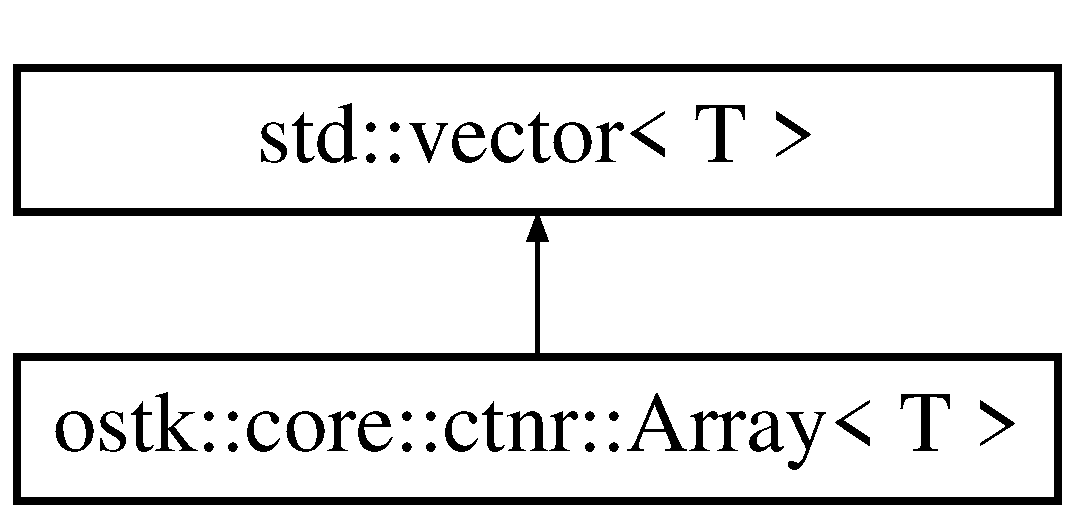
\includegraphics[height=2.000000cm]{classostk_1_1core_1_1ctnr_1_1_array}
\end{center}
\end{figure}
\subsection*{Public Types}
\begin{DoxyCompactItemize}
\item 
typedef std\+::vector$<$ T $>$\+::const\+\_\+iterator \hyperlink{classostk_1_1core_1_1ctnr_1_1_array_acf6e5ab86e3ad3e125f61b1933772a14}{Const\+Iterator}
\item 
typedef std\+::vector$<$ T $>$\+::iterator \hyperlink{classostk_1_1core_1_1ctnr_1_1_array_accf81dc56e553dad2ce7b72802836c46}{Iterator}
\item 
typedef std\+::function$<$ bool(const T \&)$>$ \hyperlink{classostk_1_1core_1_1ctnr_1_1_array_a7c04a98dd10cd625acf96addd312d0af}{Predicate}
\end{DoxyCompactItemize}
\subsection*{Public Member Functions}
\begin{DoxyCompactItemize}
\item 
\hyperlink{classostk_1_1core_1_1ctnr_1_1_array_a4e10a5235b2fa8d420dc7fd30ebb081d}{Array} ()
\begin{DoxyCompactList}\small\item\em Default constructor (disabled) \end{DoxyCompactList}\item 
\hyperlink{classostk_1_1core_1_1ctnr_1_1_array_ad26e8cf9b109bc6c821c7408cac2935b}{Array} (const std\+::vector$<$ T $>$ \&a\+Vector)
\begin{DoxyCompactList}\small\item\em Constructs an array from a C++ Standard Library vector. \end{DoxyCompactList}\item 
\hyperlink{classostk_1_1core_1_1ctnr_1_1_array_ac4ff1f3f9c03f53963ad04dedd2addf2}{Array} (const Size \&a\+Size, const T \&a\+Value)
\begin{DoxyCompactList}\small\item\em Constructs an array of given size populated with a given value. \end{DoxyCompactList}\item 
{\footnotesize template$<$class Input\+Iterator $>$ }\\\hyperlink{classostk_1_1core_1_1ctnr_1_1_array_addf98739f6a298fadcd90c7ce11848b7}{Array} (Input\+Iterator a\+First\+Iterator, Input\+Iterator a\+Last\+Iterator, const typename std\+::vector$<$ T $>$\+::allocator\+\_\+type \&an\+Allocator=typename std\+::vector$<$ T $>$\+::allocator\+\_\+type())
\item 
\hyperlink{classostk_1_1core_1_1ctnr_1_1_array_a7e03bada8d56653599563f82d8dc9895}{Array} (std\+::initializer\+\_\+list$<$ T $>$ a\+List)
\begin{DoxyCompactList}\small\item\em Constructs an array using an initializer list. \end{DoxyCompactList}\item 
\hyperlink{classostk_1_1core_1_1ctnr_1_1_array_aea744c067ca9d3f22ef7798cb977b59f}{Array} (const \hyperlink{classostk_1_1core_1_1ctnr_1_1_array}{Array} \&an\+Array)=default
\begin{DoxyCompactList}\small\item\em Copy constructor. \end{DoxyCompactList}\item 
\hyperlink{classostk_1_1core_1_1ctnr_1_1_array_a2d36f4f6bf24722cef7ccbe65d2c7927}{Array} (\hyperlink{classostk_1_1core_1_1ctnr_1_1_array}{Array} \&\&an\+Array)=default
\begin{DoxyCompactList}\small\item\em Move constructor (array) \end{DoxyCompactList}\item 
\hyperlink{classostk_1_1core_1_1ctnr_1_1_array_a45c08da536520aad843546a4996c3830}{Array} (std\+::vector$<$ T $>$ \&\&a\+Vector)
\begin{DoxyCompactList}\small\item\em Move constructor (vector) \end{DoxyCompactList}\item 
\hyperlink{classostk_1_1core_1_1ctnr_1_1_array}{Array}$<$ T $>$ \& \hyperlink{classostk_1_1core_1_1ctnr_1_1_array_af0eab66650f3f3d27c0fab8da87ebd32}{operator=} (const \hyperlink{classostk_1_1core_1_1ctnr_1_1_array}{Array}$<$ T $>$ \&an\+Array)=default
\begin{DoxyCompactList}\small\item\em Copy assignment operator. \end{DoxyCompactList}\item 
\hyperlink{classostk_1_1core_1_1ctnr_1_1_array}{Array}$<$ T $>$ \& \hyperlink{classostk_1_1core_1_1ctnr_1_1_array_a1d596aae830a46ce368d8a6cfdeba722}{operator=} (\hyperlink{classostk_1_1core_1_1ctnr_1_1_array}{Array}$<$ T $>$ \&\&an\+Array)=default
\begin{DoxyCompactList}\small\item\em Move assignment operator. \end{DoxyCompactList}\item 
\hyperlink{classostk_1_1core_1_1ctnr_1_1_array}{Array}$<$ T $>$ \hyperlink{classostk_1_1core_1_1ctnr_1_1_array_a9326348f023fe3a714249071ed185ef4}{operator+} (const \hyperlink{classostk_1_1core_1_1ctnr_1_1_array}{Array}$<$ T $>$ \&an\+Array) const
\begin{DoxyCompactList}\small\item\em Concatenate array. \end{DoxyCompactList}\item 
bool \hyperlink{classostk_1_1core_1_1ctnr_1_1_array_a8250cd3b1e3dc9b80d5d3d1ad360a5bb}{is\+Empty} () const
\begin{DoxyCompactList}\small\item\em Check if array is empty. \end{DoxyCompactList}\item 
bool \hyperlink{classostk_1_1core_1_1ctnr_1_1_array_a85fc440424ec33983e25238e9cbde67d}{contains} (const T \&an\+Element) const
\begin{DoxyCompactList}\small\item\em Check if array contains element (by value) \end{DoxyCompactList}\item 
bool \hyperlink{classostk_1_1core_1_1ctnr_1_1_array_a84e6c98f80b38dd59339eee9b8a97419}{is\+Near} (const \hyperlink{classostk_1_1core_1_1ctnr_1_1_array}{Array}$<$ T $>$ \&an\+Array, const T \&a\+Tolerance) const
\begin{DoxyCompactList}\small\item\em Check if array is near another array. \end{DoxyCompactList}\item 
bool \hyperlink{classostk_1_1core_1_1ctnr_1_1_array_a5d568e0bb551d55ff4d2ed9fbbe00c16}{is\+Near} (const \hyperlink{classostk_1_1core_1_1ctnr_1_1_array}{Array}$<$ T $>$ \&an\+Array, const std\+::function$<$ bool(const T \&, const T \&)$>$ \&a\+Comparator) const
\begin{DoxyCompactList}\small\item\em Check if array is near another array. \end{DoxyCompactList}\item 
const T \& \hyperlink{classostk_1_1core_1_1ctnr_1_1_array_ab8a576023f31f018a134831de36d5eb9}{access\+First} () const
\begin{DoxyCompactList}\small\item\em Access first element. \end{DoxyCompactList}\item 
const T \& \hyperlink{classostk_1_1core_1_1ctnr_1_1_array_a10ce6e99048cfd2fea96a934e2737604}{access\+Last} () const
\begin{DoxyCompactList}\small\item\em Access last element. \end{DoxyCompactList}\item 
Size \hyperlink{classostk_1_1core_1_1ctnr_1_1_array_a42e093c2f11de1c7a96ebd0ee6262c63}{get\+Size} () const
\begin{DoxyCompactList}\small\item\em Get array size. \end{DoxyCompactList}\item 
Index \hyperlink{classostk_1_1core_1_1ctnr_1_1_array_a15962a36fd2a4fc1e972a1b68ff7c170}{get\+Index\+Of} (const T \&an\+Element) const
\begin{DoxyCompactList}\small\item\em Get index of element (by value) \end{DoxyCompactList}\item 
\hyperlink{classostk_1_1core_1_1types_1_1_string}{types\+::\+String} \hyperlink{classostk_1_1core_1_1ctnr_1_1_array_ae37fc56c3d30592d785ea620cbcaf0ce}{to\+String} () const
\begin{DoxyCompactList}\small\item\em Get string representation of array. \end{DoxyCompactList}\item 
\hyperlink{classostk_1_1core_1_1ctnr_1_1_array}{Array}$<$ const T $\ast$ $>$ \hyperlink{classostk_1_1core_1_1ctnr_1_1_array_a13881bfc56b23de68e3d50cd07b7944e}{access\+Where} (const \hyperlink{classostk_1_1core_1_1ctnr_1_1_array}{Array}$<$ T $>$\+::\hyperlink{classostk_1_1core_1_1ctnr_1_1_array_a7c04a98dd10cd625acf96addd312d0af}{Predicate} \&a\+Predicate) const
\begin{DoxyCompactList}\small\item\em Get array of pointers to element based on condition. \end{DoxyCompactList}\item 
\hyperlink{classostk_1_1core_1_1ctnr_1_1_array}{Array}$<$ T $>$ \hyperlink{classostk_1_1core_1_1ctnr_1_1_array_adc03cfa862d43df7734e69f685534bf1}{get\+Where} (const \hyperlink{classostk_1_1core_1_1ctnr_1_1_array}{Array}$<$ T $>$\+::\hyperlink{classostk_1_1core_1_1ctnr_1_1_array_a7c04a98dd10cd625acf96addd312d0af}{Predicate} \&a\+Predicate) const
\begin{DoxyCompactList}\small\item\em Get array of elements based on condition. \end{DoxyCompactList}\item 
\hyperlink{classostk_1_1core_1_1ctnr_1_1_array}{Array}$<$ T $>$\+::\hyperlink{classostk_1_1core_1_1ctnr_1_1_array_acf6e5ab86e3ad3e125f61b1933772a14}{Const\+Iterator} \hyperlink{classostk_1_1core_1_1ctnr_1_1_array_abf965f4f2eaa744eeeafd315837ec9fb}{find} (const T \&an\+Element) const
\begin{DoxyCompactList}\small\item\em Get iterator to element, finding by by value. \end{DoxyCompactList}\item 
{\footnotesize template$<$typename U $>$ }\\\hyperlink{classostk_1_1core_1_1ctnr_1_1_array}{Array}$<$ U $>$ \hyperlink{classostk_1_1core_1_1ctnr_1_1_array_abf98d57cd72f4f544c16b1ad716858c1}{map} (const std\+::function$<$ U(T)$>$ a\+Mapping\+Function) const
\begin{DoxyCompactList}\small\item\em Get mapped array. \end{DoxyCompactList}\item 
T \hyperlink{classostk_1_1core_1_1ctnr_1_1_array_a26fb804388b4f3fad508fa1cd7867f52}{reduce} (const std\+::function$<$ T(T, T)$>$ \&a\+Reduce\+Function) const
\begin{DoxyCompactList}\small\item\em Get reduced value. \end{DoxyCompactList}\item 
T \& \hyperlink{classostk_1_1core_1_1ctnr_1_1_array_a88b92f1b1cd74fe742449a0aaa51f2fb}{access\+First} ()
\begin{DoxyCompactList}\small\item\em Access first element. \end{DoxyCompactList}\item 
T \& \hyperlink{classostk_1_1core_1_1ctnr_1_1_array_a50d0a7c9f1c121f8c6b9638663acdff3}{access\+Last} ()
\begin{DoxyCompactList}\small\item\em Access last element. \end{DoxyCompactList}\item 
void \hyperlink{classostk_1_1core_1_1ctnr_1_1_array_a3da40b4167e78eb748fa39a12cdeb21e}{add} (const T \&an\+Element)
\begin{DoxyCompactList}\small\item\em Add element to array. \end{DoxyCompactList}\item 
void \hyperlink{classostk_1_1core_1_1ctnr_1_1_array_a181587d350f45e2438583234a73b03f5}{remove} (const T \&an\+Element)
\begin{DoxyCompactList}\small\item\em Remove element from array (by value) \end{DoxyCompactList}\item 
void \hyperlink{classostk_1_1core_1_1ctnr_1_1_array_a53cc258c0052dee12217670f2bca3540}{add} (const \hyperlink{classostk_1_1core_1_1ctnr_1_1_array}{Array}$<$ T $>$ \&an\+Array)
\begin{DoxyCompactList}\small\item\em Add elements to array. \end{DoxyCompactList}\item 
void \hyperlink{classostk_1_1core_1_1ctnr_1_1_array_a9409ea2330b85382d25bc4df7c6b993f}{remove} (const \hyperlink{classostk_1_1core_1_1ctnr_1_1_array}{Array}$<$ T $>$ \&an\+Array)
\begin{DoxyCompactList}\small\item\em Remove elements from array (by value) \end{DoxyCompactList}\item 
void \hyperlink{classostk_1_1core_1_1ctnr_1_1_array_a7b436feb27e4b0c81cf218bc61b6f5f2}{merge\+With} (const \hyperlink{classostk_1_1core_1_1ctnr_1_1_array}{Array}$<$ T $>$ \&an\+Array)
\begin{DoxyCompactList}\small\item\em Merge array with another array. \end{DoxyCompactList}\item 
void \hyperlink{classostk_1_1core_1_1ctnr_1_1_array_aa4cc38300dac06710e281a3bb7fae86d}{remove\+Where} (const \hyperlink{classostk_1_1core_1_1ctnr_1_1_array}{Array}$<$ T $>$\+::\hyperlink{classostk_1_1core_1_1ctnr_1_1_array_a7c04a98dd10cd625acf96addd312d0af}{Predicate} \&a\+Predicate)
\begin{DoxyCompactList}\small\item\em Remove elements based on condition. \end{DoxyCompactList}\item 
\hyperlink{classostk_1_1core_1_1ctnr_1_1_array}{Array}$<$ T $>$\+::\hyperlink{classostk_1_1core_1_1ctnr_1_1_array_accf81dc56e553dad2ce7b72802836c46}{Iterator} \hyperlink{classostk_1_1core_1_1ctnr_1_1_array_abff2b3ec6c0a3345568ddd7c19ff5b86}{find} (const T \&an\+Element)
\begin{DoxyCompactList}\small\item\em Get iterator to element, finding by value. \end{DoxyCompactList}\end{DoxyCompactItemize}
\subsection*{Static Public Member Functions}
\begin{DoxyCompactItemize}
\item 
static \hyperlink{classostk_1_1core_1_1ctnr_1_1_array}{Array}$<$ T $>$ \hyperlink{classostk_1_1core_1_1ctnr_1_1_array_a0d6dc521540ee128b43a66663c9f3dd8}{Empty} ()
\begin{DoxyCompactList}\small\item\em Constructs an empty array. \end{DoxyCompactList}\end{DoxyCompactItemize}
\subsection*{Friends}
\begin{DoxyCompactItemize}
\item 
{\footnotesize template$<$class U $>$ }\\std\+::ostream \& \hyperlink{classostk_1_1core_1_1ctnr_1_1_array_a9daa2d638e5bd693776f8bf6caae0802}{operator$<$$<$} (std\+::ostream \&an\+Output\+Stream, const \hyperlink{classostk_1_1core_1_1ctnr_1_1_array}{Array}$<$ U $>$ \&an\+Array)
\begin{DoxyCompactList}\small\item\em Output stream operator. \end{DoxyCompactList}\end{DoxyCompactItemize}


\subsection{Detailed Description}
\subsubsection*{template$<$class T$>$\newline
class ostk\+::core\+::ctnr\+::\+Array$<$ T $>$}

\hyperlink{classostk_1_1core_1_1ctnr_1_1_array}{Array} container. 

Sequence containers representing arrays that can change in size. Arrays use contiguous storage locations for their elements. 

\subsection{Member Typedef Documentation}
\mbox{\Hypertarget{classostk_1_1core_1_1ctnr_1_1_array_acf6e5ab86e3ad3e125f61b1933772a14}\label{classostk_1_1core_1_1ctnr_1_1_array_acf6e5ab86e3ad3e125f61b1933772a14}} 
\index{ostk\+::core\+::ctnr\+::\+Array@{ostk\+::core\+::ctnr\+::\+Array}!Const\+Iterator@{Const\+Iterator}}
\index{Const\+Iterator@{Const\+Iterator}!ostk\+::core\+::ctnr\+::\+Array@{ostk\+::core\+::ctnr\+::\+Array}}
\subsubsection{\texorpdfstring{Const\+Iterator}{ConstIterator}}
{\footnotesize\ttfamily template$<$class T$>$ \\
typedef std\+::vector$<$T$>$\+::const\+\_\+iterator \hyperlink{classostk_1_1core_1_1ctnr_1_1_array}{ostk\+::core\+::ctnr\+::\+Array}$<$ T $>$\+::\hyperlink{classostk_1_1core_1_1ctnr_1_1_array_acf6e5ab86e3ad3e125f61b1933772a14}{Const\+Iterator}}

\mbox{\Hypertarget{classostk_1_1core_1_1ctnr_1_1_array_accf81dc56e553dad2ce7b72802836c46}\label{classostk_1_1core_1_1ctnr_1_1_array_accf81dc56e553dad2ce7b72802836c46}} 
\index{ostk\+::core\+::ctnr\+::\+Array@{ostk\+::core\+::ctnr\+::\+Array}!Iterator@{Iterator}}
\index{Iterator@{Iterator}!ostk\+::core\+::ctnr\+::\+Array@{ostk\+::core\+::ctnr\+::\+Array}}
\subsubsection{\texorpdfstring{Iterator}{Iterator}}
{\footnotesize\ttfamily template$<$class T$>$ \\
typedef std\+::vector$<$T$>$\+::iterator \hyperlink{classostk_1_1core_1_1ctnr_1_1_array}{ostk\+::core\+::ctnr\+::\+Array}$<$ T $>$\+::\hyperlink{classostk_1_1core_1_1ctnr_1_1_array_accf81dc56e553dad2ce7b72802836c46}{Iterator}}

\mbox{\Hypertarget{classostk_1_1core_1_1ctnr_1_1_array_a7c04a98dd10cd625acf96addd312d0af}\label{classostk_1_1core_1_1ctnr_1_1_array_a7c04a98dd10cd625acf96addd312d0af}} 
\index{ostk\+::core\+::ctnr\+::\+Array@{ostk\+::core\+::ctnr\+::\+Array}!Predicate@{Predicate}}
\index{Predicate@{Predicate}!ostk\+::core\+::ctnr\+::\+Array@{ostk\+::core\+::ctnr\+::\+Array}}
\subsubsection{\texorpdfstring{Predicate}{Predicate}}
{\footnotesize\ttfamily template$<$class T$>$ \\
typedef std\+::function$<$bool(const T\&)$>$ \hyperlink{classostk_1_1core_1_1ctnr_1_1_array}{ostk\+::core\+::ctnr\+::\+Array}$<$ T $>$\+::\hyperlink{classostk_1_1core_1_1ctnr_1_1_array_a7c04a98dd10cd625acf96addd312d0af}{Predicate}}



\subsection{Constructor \& Destructor Documentation}
\mbox{\Hypertarget{classostk_1_1core_1_1ctnr_1_1_array_a4e10a5235b2fa8d420dc7fd30ebb081d}\label{classostk_1_1core_1_1ctnr_1_1_array_a4e10a5235b2fa8d420dc7fd30ebb081d}} 
\index{ostk\+::core\+::ctnr\+::\+Array@{ostk\+::core\+::ctnr\+::\+Array}!Array@{Array}}
\index{Array@{Array}!ostk\+::core\+::ctnr\+::\+Array@{ostk\+::core\+::ctnr\+::\+Array}}
\subsubsection{\texorpdfstring{Array()}{Array()}\hspace{0.1cm}{\footnotesize\ttfamily [1/8]}}
{\footnotesize\ttfamily template$<$class T$>$ \\
\hyperlink{classostk_1_1core_1_1ctnr_1_1_array}{ostk\+::core\+::ctnr\+::\+Array}$<$ T $>$\+::\hyperlink{classostk_1_1core_1_1ctnr_1_1_array}{Array} (\begin{DoxyParamCaption}{ }\end{DoxyParamCaption})}



Default constructor (disabled) 

\mbox{\Hypertarget{classostk_1_1core_1_1ctnr_1_1_array_ad26e8cf9b109bc6c821c7408cac2935b}\label{classostk_1_1core_1_1ctnr_1_1_array_ad26e8cf9b109bc6c821c7408cac2935b}} 
\index{ostk\+::core\+::ctnr\+::\+Array@{ostk\+::core\+::ctnr\+::\+Array}!Array@{Array}}
\index{Array@{Array}!ostk\+::core\+::ctnr\+::\+Array@{ostk\+::core\+::ctnr\+::\+Array}}
\subsubsection{\texorpdfstring{Array()}{Array()}\hspace{0.1cm}{\footnotesize\ttfamily [2/8]}}
{\footnotesize\ttfamily template$<$class T$>$ \\
\hyperlink{classostk_1_1core_1_1ctnr_1_1_array}{ostk\+::core\+::ctnr\+::\+Array}$<$ T $>$\+::\hyperlink{classostk_1_1core_1_1ctnr_1_1_array}{Array} (\begin{DoxyParamCaption}\item[{const std\+::vector$<$ T $>$ \&}]{a\+Vector }\end{DoxyParamCaption})}



Constructs an array from a C++ Standard Library vector. 


\begin{DoxyCode}
std::vector<Integer> vector = \{1, 2, 3\} ;
Array<Integer> array(vector) ;
\end{DoxyCode}



\begin{DoxyParams}[1]{Parameters}
\mbox{\tt in}  & {\em a\+Vector} & A vector \\
\hline
\end{DoxyParams}
\mbox{\Hypertarget{classostk_1_1core_1_1ctnr_1_1_array_ac4ff1f3f9c03f53963ad04dedd2addf2}\label{classostk_1_1core_1_1ctnr_1_1_array_ac4ff1f3f9c03f53963ad04dedd2addf2}} 
\index{ostk\+::core\+::ctnr\+::\+Array@{ostk\+::core\+::ctnr\+::\+Array}!Array@{Array}}
\index{Array@{Array}!ostk\+::core\+::ctnr\+::\+Array@{ostk\+::core\+::ctnr\+::\+Array}}
\subsubsection{\texorpdfstring{Array()}{Array()}\hspace{0.1cm}{\footnotesize\ttfamily [3/8]}}
{\footnotesize\ttfamily template$<$class T$>$ \\
\hyperlink{classostk_1_1core_1_1ctnr_1_1_array}{ostk\+::core\+::ctnr\+::\+Array}$<$ T $>$\+::\hyperlink{classostk_1_1core_1_1ctnr_1_1_array}{Array} (\begin{DoxyParamCaption}\item[{const Size \&}]{a\+Size,  }\item[{const T \&}]{a\+Value }\end{DoxyParamCaption})}



Constructs an array of given size populated with a given value. 


\begin{DoxyCode}
Array<String> array(3, \textcolor{stringliteral}{"abc"}) ; \textcolor{comment}{// ["abc", "abc", "abc"]}
\end{DoxyCode}



\begin{DoxyParams}[1]{Parameters}
\mbox{\tt in}  & {\em a\+Size} & An array size \\
\hline
\mbox{\tt in}  & {\em a\+Value} & A value \\
\hline
\end{DoxyParams}
\mbox{\Hypertarget{classostk_1_1core_1_1ctnr_1_1_array_addf98739f6a298fadcd90c7ce11848b7}\label{classostk_1_1core_1_1ctnr_1_1_array_addf98739f6a298fadcd90c7ce11848b7}} 
\index{ostk\+::core\+::ctnr\+::\+Array@{ostk\+::core\+::ctnr\+::\+Array}!Array@{Array}}
\index{Array@{Array}!ostk\+::core\+::ctnr\+::\+Array@{ostk\+::core\+::ctnr\+::\+Array}}
\subsubsection{\texorpdfstring{Array()}{Array()}\hspace{0.1cm}{\footnotesize\ttfamily [4/8]}}
{\footnotesize\ttfamily template$<$class T$>$ \\
template$<$class Input\+Iterator $>$ \\
\hyperlink{classostk_1_1core_1_1ctnr_1_1_array}{ostk\+::core\+::ctnr\+::\+Array}$<$ T $>$\+::\hyperlink{classostk_1_1core_1_1ctnr_1_1_array}{Array} (\begin{DoxyParamCaption}\item[{Input\+Iterator}]{a\+First\+Iterator,  }\item[{Input\+Iterator}]{a\+Last\+Iterator,  }\item[{const typename std\+::vector$<$ T $>$\+::allocator\+\_\+type \&}]{an\+Allocator = {\ttfamily typename~std\+:\+:vector$<$~T~$>$\+:\+:allocator\+\_\+type()} }\end{DoxyParamCaption})}

\mbox{\Hypertarget{classostk_1_1core_1_1ctnr_1_1_array_a7e03bada8d56653599563f82d8dc9895}\label{classostk_1_1core_1_1ctnr_1_1_array_a7e03bada8d56653599563f82d8dc9895}} 
\index{ostk\+::core\+::ctnr\+::\+Array@{ostk\+::core\+::ctnr\+::\+Array}!Array@{Array}}
\index{Array@{Array}!ostk\+::core\+::ctnr\+::\+Array@{ostk\+::core\+::ctnr\+::\+Array}}
\subsubsection{\texorpdfstring{Array()}{Array()}\hspace{0.1cm}{\footnotesize\ttfamily [5/8]}}
{\footnotesize\ttfamily template$<$class T$>$ \\
\hyperlink{classostk_1_1core_1_1ctnr_1_1_array}{ostk\+::core\+::ctnr\+::\+Array}$<$ T $>$\+::\hyperlink{classostk_1_1core_1_1ctnr_1_1_array}{Array} (\begin{DoxyParamCaption}\item[{std\+::initializer\+\_\+list$<$ T $>$}]{a\+List }\end{DoxyParamCaption})}



Constructs an array using an initializer list. 


\begin{DoxyCode}
Array<Integer> array = \{1, 2, 3\} ;
\end{DoxyCode}



\begin{DoxyParams}[1]{Parameters}
\mbox{\tt in}  & {\em a\+List} & An initializer list \\
\hline
\end{DoxyParams}
\mbox{\Hypertarget{classostk_1_1core_1_1ctnr_1_1_array_aea744c067ca9d3f22ef7798cb977b59f}\label{classostk_1_1core_1_1ctnr_1_1_array_aea744c067ca9d3f22ef7798cb977b59f}} 
\index{ostk\+::core\+::ctnr\+::\+Array@{ostk\+::core\+::ctnr\+::\+Array}!Array@{Array}}
\index{Array@{Array}!ostk\+::core\+::ctnr\+::\+Array@{ostk\+::core\+::ctnr\+::\+Array}}
\subsubsection{\texorpdfstring{Array()}{Array()}\hspace{0.1cm}{\footnotesize\ttfamily [6/8]}}
{\footnotesize\ttfamily template$<$class T$>$ \\
\hyperlink{classostk_1_1core_1_1ctnr_1_1_array}{ostk\+::core\+::ctnr\+::\+Array}$<$ T $>$\+::\hyperlink{classostk_1_1core_1_1ctnr_1_1_array}{Array} (\begin{DoxyParamCaption}\item[{const \hyperlink{classostk_1_1core_1_1ctnr_1_1_array}{Array}$<$ T $>$ \&}]{an\+Array }\end{DoxyParamCaption})\hspace{0.3cm}{\ttfamily [default]}}



Copy constructor. 


\begin{DoxyParams}[1]{Parameters}
\mbox{\tt in}  & {\em an\+Array} & An array \\
\hline
\end{DoxyParams}
\mbox{\Hypertarget{classostk_1_1core_1_1ctnr_1_1_array_a2d36f4f6bf24722cef7ccbe65d2c7927}\label{classostk_1_1core_1_1ctnr_1_1_array_a2d36f4f6bf24722cef7ccbe65d2c7927}} 
\index{ostk\+::core\+::ctnr\+::\+Array@{ostk\+::core\+::ctnr\+::\+Array}!Array@{Array}}
\index{Array@{Array}!ostk\+::core\+::ctnr\+::\+Array@{ostk\+::core\+::ctnr\+::\+Array}}
\subsubsection{\texorpdfstring{Array()}{Array()}\hspace{0.1cm}{\footnotesize\ttfamily [7/8]}}
{\footnotesize\ttfamily template$<$class T$>$ \\
\hyperlink{classostk_1_1core_1_1ctnr_1_1_array}{ostk\+::core\+::ctnr\+::\+Array}$<$ T $>$\+::\hyperlink{classostk_1_1core_1_1ctnr_1_1_array}{Array} (\begin{DoxyParamCaption}\item[{\hyperlink{classostk_1_1core_1_1ctnr_1_1_array}{Array}$<$ T $>$ \&\&}]{an\+Array }\end{DoxyParamCaption})\hspace{0.3cm}{\ttfamily [default]}}



Move constructor (array) 


\begin{DoxyParams}[1]{Parameters}
\mbox{\tt in}  & {\em an\+Array} & An array \\
\hline
\end{DoxyParams}
\mbox{\Hypertarget{classostk_1_1core_1_1ctnr_1_1_array_a45c08da536520aad843546a4996c3830}\label{classostk_1_1core_1_1ctnr_1_1_array_a45c08da536520aad843546a4996c3830}} 
\index{ostk\+::core\+::ctnr\+::\+Array@{ostk\+::core\+::ctnr\+::\+Array}!Array@{Array}}
\index{Array@{Array}!ostk\+::core\+::ctnr\+::\+Array@{ostk\+::core\+::ctnr\+::\+Array}}
\subsubsection{\texorpdfstring{Array()}{Array()}\hspace{0.1cm}{\footnotesize\ttfamily [8/8]}}
{\footnotesize\ttfamily template$<$class T$>$ \\
\hyperlink{classostk_1_1core_1_1ctnr_1_1_array}{ostk\+::core\+::ctnr\+::\+Array}$<$ T $>$\+::\hyperlink{classostk_1_1core_1_1ctnr_1_1_array}{Array} (\begin{DoxyParamCaption}\item[{std\+::vector$<$ T $>$ \&\&}]{a\+Vector }\end{DoxyParamCaption})}



Move constructor (vector) 


\begin{DoxyParams}[1]{Parameters}
\mbox{\tt in}  & {\em a\+Vector} & A vector \\
\hline
\end{DoxyParams}


\subsection{Member Function Documentation}
\mbox{\Hypertarget{classostk_1_1core_1_1ctnr_1_1_array_ab8a576023f31f018a134831de36d5eb9}\label{classostk_1_1core_1_1ctnr_1_1_array_ab8a576023f31f018a134831de36d5eb9}} 
\index{ostk\+::core\+::ctnr\+::\+Array@{ostk\+::core\+::ctnr\+::\+Array}!access\+First@{access\+First}}
\index{access\+First@{access\+First}!ostk\+::core\+::ctnr\+::\+Array@{ostk\+::core\+::ctnr\+::\+Array}}
\subsubsection{\texorpdfstring{access\+First()}{accessFirst()}\hspace{0.1cm}{\footnotesize\ttfamily [1/2]}}
{\footnotesize\ttfamily template$<$class T$>$ \\
const T\& \hyperlink{classostk_1_1core_1_1ctnr_1_1_array}{ostk\+::core\+::ctnr\+::\+Array}$<$ T $>$\+::access\+First (\begin{DoxyParamCaption}{ }\end{DoxyParamCaption}) const}



Access first element. 


\begin{DoxyCode}
Array<Integer> array = \{1, 2, 3\} ;
\textcolor{keyword}{const} Integer& element = array.accessFirst() ; \textcolor{comment}{// 1}
\end{DoxyCode}


\begin{DoxyReturn}{Returns}
Reference to the first element of array 
\end{DoxyReturn}
\mbox{\Hypertarget{classostk_1_1core_1_1ctnr_1_1_array_a88b92f1b1cd74fe742449a0aaa51f2fb}\label{classostk_1_1core_1_1ctnr_1_1_array_a88b92f1b1cd74fe742449a0aaa51f2fb}} 
\index{ostk\+::core\+::ctnr\+::\+Array@{ostk\+::core\+::ctnr\+::\+Array}!access\+First@{access\+First}}
\index{access\+First@{access\+First}!ostk\+::core\+::ctnr\+::\+Array@{ostk\+::core\+::ctnr\+::\+Array}}
\subsubsection{\texorpdfstring{access\+First()}{accessFirst()}\hspace{0.1cm}{\footnotesize\ttfamily [2/2]}}
{\footnotesize\ttfamily template$<$class T$>$ \\
T\& \hyperlink{classostk_1_1core_1_1ctnr_1_1_array}{ostk\+::core\+::ctnr\+::\+Array}$<$ T $>$\+::access\+First (\begin{DoxyParamCaption}{ }\end{DoxyParamCaption})}



Access first element. 


\begin{DoxyCode}
Array<Integer> array = \{1, 2, 3\} ;
Integer& element = array.accessFirst() ; \textcolor{comment}{// 1}
\end{DoxyCode}


\begin{DoxyReturn}{Returns}
Reference to the first element of array 
\end{DoxyReturn}
\mbox{\Hypertarget{classostk_1_1core_1_1ctnr_1_1_array_a10ce6e99048cfd2fea96a934e2737604}\label{classostk_1_1core_1_1ctnr_1_1_array_a10ce6e99048cfd2fea96a934e2737604}} 
\index{ostk\+::core\+::ctnr\+::\+Array@{ostk\+::core\+::ctnr\+::\+Array}!access\+Last@{access\+Last}}
\index{access\+Last@{access\+Last}!ostk\+::core\+::ctnr\+::\+Array@{ostk\+::core\+::ctnr\+::\+Array}}
\subsubsection{\texorpdfstring{access\+Last()}{accessLast()}\hspace{0.1cm}{\footnotesize\ttfamily [1/2]}}
{\footnotesize\ttfamily template$<$class T$>$ \\
const T\& \hyperlink{classostk_1_1core_1_1ctnr_1_1_array}{ostk\+::core\+::ctnr\+::\+Array}$<$ T $>$\+::access\+Last (\begin{DoxyParamCaption}{ }\end{DoxyParamCaption}) const}



Access last element. 


\begin{DoxyCode}
Array<Integer> array = \{1, 2, 3\} ;
\textcolor{keyword}{const} Integer& element = array.accessLast() ; \textcolor{comment}{// 3}
\end{DoxyCode}


\begin{DoxyReturn}{Returns}
Reference to the last element of array 
\end{DoxyReturn}
\mbox{\Hypertarget{classostk_1_1core_1_1ctnr_1_1_array_a50d0a7c9f1c121f8c6b9638663acdff3}\label{classostk_1_1core_1_1ctnr_1_1_array_a50d0a7c9f1c121f8c6b9638663acdff3}} 
\index{ostk\+::core\+::ctnr\+::\+Array@{ostk\+::core\+::ctnr\+::\+Array}!access\+Last@{access\+Last}}
\index{access\+Last@{access\+Last}!ostk\+::core\+::ctnr\+::\+Array@{ostk\+::core\+::ctnr\+::\+Array}}
\subsubsection{\texorpdfstring{access\+Last()}{accessLast()}\hspace{0.1cm}{\footnotesize\ttfamily [2/2]}}
{\footnotesize\ttfamily template$<$class T$>$ \\
T\& \hyperlink{classostk_1_1core_1_1ctnr_1_1_array}{ostk\+::core\+::ctnr\+::\+Array}$<$ T $>$\+::access\+Last (\begin{DoxyParamCaption}{ }\end{DoxyParamCaption})}



Access last element. 


\begin{DoxyCode}
Array<Integer> array = \{1, 2, 3\} ;
Integer& element = array.accessLast() ; \textcolor{comment}{// 3}
\end{DoxyCode}


\begin{DoxyReturn}{Returns}
Reference to the last element of array 
\end{DoxyReturn}
\mbox{\Hypertarget{classostk_1_1core_1_1ctnr_1_1_array_a13881bfc56b23de68e3d50cd07b7944e}\label{classostk_1_1core_1_1ctnr_1_1_array_a13881bfc56b23de68e3d50cd07b7944e}} 
\index{ostk\+::core\+::ctnr\+::\+Array@{ostk\+::core\+::ctnr\+::\+Array}!access\+Where@{access\+Where}}
\index{access\+Where@{access\+Where}!ostk\+::core\+::ctnr\+::\+Array@{ostk\+::core\+::ctnr\+::\+Array}}
\subsubsection{\texorpdfstring{access\+Where()}{accessWhere()}}
{\footnotesize\ttfamily template$<$class T$>$ \\
\hyperlink{classostk_1_1core_1_1ctnr_1_1_array}{Array}$<$const T$\ast$$>$ \hyperlink{classostk_1_1core_1_1ctnr_1_1_array}{ostk\+::core\+::ctnr\+::\+Array}$<$ T $>$\+::access\+Where (\begin{DoxyParamCaption}\item[{const \hyperlink{classostk_1_1core_1_1ctnr_1_1_array}{Array}$<$ T $>$\+::\hyperlink{classostk_1_1core_1_1ctnr_1_1_array_a7c04a98dd10cd625acf96addd312d0af}{Predicate} \&}]{a\+Predicate }\end{DoxyParamCaption}) const}



Get array of pointers to element based on condition. 


\begin{DoxyCode}
Array<Integer> array = \{0, 1, 2, 3, 4\} ;
Array<const Integer*> elements = array.accessWhere([] (\textcolor{keyword}{const} Integer& anInteger) -> \textcolor{keywordtype}{bool} \{ \textcolor{keywordflow}{return} anInteger
      .isEven() ; \}) ; \textcolor{comment}{// [&0, &2, &4]}
\end{DoxyCode}



\begin{DoxyParams}[1]{Parameters}
\mbox{\tt in}  & {\em a\+Predicate} & A predicate \\
\hline
\end{DoxyParams}
\begin{DoxyReturn}{Returns}
\hyperlink{classostk_1_1core_1_1ctnr_1_1_array}{Array} of pointers to element 
\end{DoxyReturn}
\mbox{\Hypertarget{classostk_1_1core_1_1ctnr_1_1_array_a3da40b4167e78eb748fa39a12cdeb21e}\label{classostk_1_1core_1_1ctnr_1_1_array_a3da40b4167e78eb748fa39a12cdeb21e}} 
\index{ostk\+::core\+::ctnr\+::\+Array@{ostk\+::core\+::ctnr\+::\+Array}!add@{add}}
\index{add@{add}!ostk\+::core\+::ctnr\+::\+Array@{ostk\+::core\+::ctnr\+::\+Array}}
\subsubsection{\texorpdfstring{add()}{add()}\hspace{0.1cm}{\footnotesize\ttfamily [1/2]}}
{\footnotesize\ttfamily template$<$class T$>$ \\
void \hyperlink{classostk_1_1core_1_1ctnr_1_1_array}{ostk\+::core\+::ctnr\+::\+Array}$<$ T $>$\+::add (\begin{DoxyParamCaption}\item[{const T \&}]{an\+Element }\end{DoxyParamCaption})}



Add element to array. 


\begin{DoxyCode}
Array<Integer> array = \{1, 2, 3\} ;
array.add(4) ; \textcolor{comment}{// [1, 2, 3, 4]}
\end{DoxyCode}



\begin{DoxyParams}[1]{Parameters}
\mbox{\tt in}  & {\em an\+Element} & An element \\
\hline
\end{DoxyParams}
\mbox{\Hypertarget{classostk_1_1core_1_1ctnr_1_1_array_a53cc258c0052dee12217670f2bca3540}\label{classostk_1_1core_1_1ctnr_1_1_array_a53cc258c0052dee12217670f2bca3540}} 
\index{ostk\+::core\+::ctnr\+::\+Array@{ostk\+::core\+::ctnr\+::\+Array}!add@{add}}
\index{add@{add}!ostk\+::core\+::ctnr\+::\+Array@{ostk\+::core\+::ctnr\+::\+Array}}
\subsubsection{\texorpdfstring{add()}{add()}\hspace{0.1cm}{\footnotesize\ttfamily [2/2]}}
{\footnotesize\ttfamily template$<$class T$>$ \\
void \hyperlink{classostk_1_1core_1_1ctnr_1_1_array}{ostk\+::core\+::ctnr\+::\+Array}$<$ T $>$\+::add (\begin{DoxyParamCaption}\item[{const \hyperlink{classostk_1_1core_1_1ctnr_1_1_array}{Array}$<$ T $>$ \&}]{an\+Array }\end{DoxyParamCaption})}



Add elements to array. 


\begin{DoxyCode}
Array<Integer> array = \{1, 2, 3\} ;
array.add(\{4, 5\}) ; \textcolor{comment}{// [1, 2, 3, 4, 5]}
\end{DoxyCode}



\begin{DoxyParams}[1]{Parameters}
\mbox{\tt in}  & {\em an\+Array} & An array of elements \\
\hline
\end{DoxyParams}
\mbox{\Hypertarget{classostk_1_1core_1_1ctnr_1_1_array_a85fc440424ec33983e25238e9cbde67d}\label{classostk_1_1core_1_1ctnr_1_1_array_a85fc440424ec33983e25238e9cbde67d}} 
\index{ostk\+::core\+::ctnr\+::\+Array@{ostk\+::core\+::ctnr\+::\+Array}!contains@{contains}}
\index{contains@{contains}!ostk\+::core\+::ctnr\+::\+Array@{ostk\+::core\+::ctnr\+::\+Array}}
\subsubsection{\texorpdfstring{contains()}{contains()}}
{\footnotesize\ttfamily template$<$class T$>$ \\
bool \hyperlink{classostk_1_1core_1_1ctnr_1_1_array}{ostk\+::core\+::ctnr\+::\+Array}$<$ T $>$\+::contains (\begin{DoxyParamCaption}\item[{const T \&}]{an\+Element }\end{DoxyParamCaption}) const}



Check if array contains element (by value) 


\begin{DoxyCode}
Array<Integer> array = \{1, 2, 3\} ;
array.contains(2) ; \textcolor{comment}{// True}
\end{DoxyCode}



\begin{DoxyParams}[1]{Parameters}
\mbox{\tt in}  & {\em an\+Element} & An element \\
\hline
\end{DoxyParams}
\begin{DoxyReturn}{Returns}
True if array contains element (by value) 
\end{DoxyReturn}
\mbox{\Hypertarget{classostk_1_1core_1_1ctnr_1_1_array_a0d6dc521540ee128b43a66663c9f3dd8}\label{classostk_1_1core_1_1ctnr_1_1_array_a0d6dc521540ee128b43a66663c9f3dd8}} 
\index{ostk\+::core\+::ctnr\+::\+Array@{ostk\+::core\+::ctnr\+::\+Array}!Empty@{Empty}}
\index{Empty@{Empty}!ostk\+::core\+::ctnr\+::\+Array@{ostk\+::core\+::ctnr\+::\+Array}}
\subsubsection{\texorpdfstring{Empty()}{Empty()}}
{\footnotesize\ttfamily template$<$class T$>$ \\
static \hyperlink{classostk_1_1core_1_1ctnr_1_1_array}{Array}$<$T$>$ \hyperlink{classostk_1_1core_1_1ctnr_1_1_array}{ostk\+::core\+::ctnr\+::\+Array}$<$ T $>$\+::Empty (\begin{DoxyParamCaption}{ }\end{DoxyParamCaption})\hspace{0.3cm}{\ttfamily [static]}}



Constructs an empty array. 


\begin{DoxyCode}
Array<Integer> array = \hyperlink{classostk_1_1core_1_1ctnr_1_1_array_a0d6dc521540ee128b43a66663c9f3dd8}{Array<Integer>::Empty}() ;
\end{DoxyCode}


\begin{DoxyReturn}{Returns}
Empty array 
\end{DoxyReturn}
\mbox{\Hypertarget{classostk_1_1core_1_1ctnr_1_1_array_abf965f4f2eaa744eeeafd315837ec9fb}\label{classostk_1_1core_1_1ctnr_1_1_array_abf965f4f2eaa744eeeafd315837ec9fb}} 
\index{ostk\+::core\+::ctnr\+::\+Array@{ostk\+::core\+::ctnr\+::\+Array}!find@{find}}
\index{find@{find}!ostk\+::core\+::ctnr\+::\+Array@{ostk\+::core\+::ctnr\+::\+Array}}
\subsubsection{\texorpdfstring{find()}{find()}\hspace{0.1cm}{\footnotesize\ttfamily [1/2]}}
{\footnotesize\ttfamily template$<$class T$>$ \\
\hyperlink{classostk_1_1core_1_1ctnr_1_1_array}{Array}$<$T$>$\+::\hyperlink{classostk_1_1core_1_1ctnr_1_1_array_acf6e5ab86e3ad3e125f61b1933772a14}{Const\+Iterator} \hyperlink{classostk_1_1core_1_1ctnr_1_1_array}{ostk\+::core\+::ctnr\+::\+Array}$<$ T $>$\+::find (\begin{DoxyParamCaption}\item[{const T \&}]{an\+Element }\end{DoxyParamCaption}) const}



Get iterator to element, finding by by value. 


\begin{DoxyCode}
Array<Integer> array = \{0, 1, 2, 3, 4\} ;
\textcolor{keyword}{auto} elementIt = array.find(2) ;
\end{DoxyCode}



\begin{DoxyParams}[1]{Parameters}
\mbox{\tt in}  & {\em an\+Element} & An element \\
\hline
\end{DoxyParams}
\begin{DoxyReturn}{Returns}
Iterator to element 
\end{DoxyReturn}
\mbox{\Hypertarget{classostk_1_1core_1_1ctnr_1_1_array_abff2b3ec6c0a3345568ddd7c19ff5b86}\label{classostk_1_1core_1_1ctnr_1_1_array_abff2b3ec6c0a3345568ddd7c19ff5b86}} 
\index{ostk\+::core\+::ctnr\+::\+Array@{ostk\+::core\+::ctnr\+::\+Array}!find@{find}}
\index{find@{find}!ostk\+::core\+::ctnr\+::\+Array@{ostk\+::core\+::ctnr\+::\+Array}}
\subsubsection{\texorpdfstring{find()}{find()}\hspace{0.1cm}{\footnotesize\ttfamily [2/2]}}
{\footnotesize\ttfamily template$<$class T$>$ \\
\hyperlink{classostk_1_1core_1_1ctnr_1_1_array}{Array}$<$T$>$\+::\hyperlink{classostk_1_1core_1_1ctnr_1_1_array_accf81dc56e553dad2ce7b72802836c46}{Iterator} \hyperlink{classostk_1_1core_1_1ctnr_1_1_array}{ostk\+::core\+::ctnr\+::\+Array}$<$ T $>$\+::find (\begin{DoxyParamCaption}\item[{const T \&}]{an\+Element }\end{DoxyParamCaption})}



Get iterator to element, finding by value. 


\begin{DoxyCode}
Array<Integer> array = \{0, 1, 2, 3, 4\} ;
\textcolor{keyword}{auto} elementIt = array.find(2) ;
\end{DoxyCode}



\begin{DoxyParams}[1]{Parameters}
\mbox{\tt in}  & {\em an\+Element} & An element \\
\hline
\end{DoxyParams}
\begin{DoxyReturn}{Returns}
Iterator to element 
\end{DoxyReturn}
\mbox{\Hypertarget{classostk_1_1core_1_1ctnr_1_1_array_a15962a36fd2a4fc1e972a1b68ff7c170}\label{classostk_1_1core_1_1ctnr_1_1_array_a15962a36fd2a4fc1e972a1b68ff7c170}} 
\index{ostk\+::core\+::ctnr\+::\+Array@{ostk\+::core\+::ctnr\+::\+Array}!get\+Index\+Of@{get\+Index\+Of}}
\index{get\+Index\+Of@{get\+Index\+Of}!ostk\+::core\+::ctnr\+::\+Array@{ostk\+::core\+::ctnr\+::\+Array}}
\subsubsection{\texorpdfstring{get\+Index\+Of()}{getIndexOf()}}
{\footnotesize\ttfamily template$<$class T$>$ \\
Index \hyperlink{classostk_1_1core_1_1ctnr_1_1_array}{ostk\+::core\+::ctnr\+::\+Array}$<$ T $>$\+::get\+Index\+Of (\begin{DoxyParamCaption}\item[{const T \&}]{an\+Element }\end{DoxyParamCaption}) const}



Get index of element (by value) 


\begin{DoxyCode}
Array<Integer> array = \{1, 2, 3\} ;
\hyperlink{namespaceostk_1_1core_1_1types_a6e63c1b15b2e5bc87a43771c09fa913a}{Index} index = array.getIndexOf(2) ; \textcolor{comment}{// 1}
\end{DoxyCode}



\begin{DoxyParams}[1]{Parameters}
\mbox{\tt in}  & {\em an\+Element} & An element \\
\hline
\end{DoxyParams}
\begin{DoxyReturn}{Returns}
Index of element (by value) 
\end{DoxyReturn}
\mbox{\Hypertarget{classostk_1_1core_1_1ctnr_1_1_array_a42e093c2f11de1c7a96ebd0ee6262c63}\label{classostk_1_1core_1_1ctnr_1_1_array_a42e093c2f11de1c7a96ebd0ee6262c63}} 
\index{ostk\+::core\+::ctnr\+::\+Array@{ostk\+::core\+::ctnr\+::\+Array}!get\+Size@{get\+Size}}
\index{get\+Size@{get\+Size}!ostk\+::core\+::ctnr\+::\+Array@{ostk\+::core\+::ctnr\+::\+Array}}
\subsubsection{\texorpdfstring{get\+Size()}{getSize()}}
{\footnotesize\ttfamily template$<$class T$>$ \\
Size \hyperlink{classostk_1_1core_1_1ctnr_1_1_array}{ostk\+::core\+::ctnr\+::\+Array}$<$ T $>$\+::get\+Size (\begin{DoxyParamCaption}{ }\end{DoxyParamCaption}) const}



Get array size. 


\begin{DoxyCode}
Array<Integer> array = \{1, 2, 3\} ;
\hyperlink{namespaceostk_1_1core_1_1types_acf68f214a245e35a7c1994c84dc56746}{Size} size = array.getSize() ; \textcolor{comment}{// 3}
\end{DoxyCode}


\begin{DoxyReturn}{Returns}
\hyperlink{classostk_1_1core_1_1ctnr_1_1_array}{Array} size 
\end{DoxyReturn}
\mbox{\Hypertarget{classostk_1_1core_1_1ctnr_1_1_array_adc03cfa862d43df7734e69f685534bf1}\label{classostk_1_1core_1_1ctnr_1_1_array_adc03cfa862d43df7734e69f685534bf1}} 
\index{ostk\+::core\+::ctnr\+::\+Array@{ostk\+::core\+::ctnr\+::\+Array}!get\+Where@{get\+Where}}
\index{get\+Where@{get\+Where}!ostk\+::core\+::ctnr\+::\+Array@{ostk\+::core\+::ctnr\+::\+Array}}
\subsubsection{\texorpdfstring{get\+Where()}{getWhere()}}
{\footnotesize\ttfamily template$<$class T$>$ \\
\hyperlink{classostk_1_1core_1_1ctnr_1_1_array}{Array}$<$T$>$ \hyperlink{classostk_1_1core_1_1ctnr_1_1_array}{ostk\+::core\+::ctnr\+::\+Array}$<$ T $>$\+::get\+Where (\begin{DoxyParamCaption}\item[{const \hyperlink{classostk_1_1core_1_1ctnr_1_1_array}{Array}$<$ T $>$\+::\hyperlink{classostk_1_1core_1_1ctnr_1_1_array_a7c04a98dd10cd625acf96addd312d0af}{Predicate} \&}]{a\+Predicate }\end{DoxyParamCaption}) const}



Get array of elements based on condition. 


\begin{DoxyCode}
Array<Integer> array = \{0, 1, 2, 3, 4\} ;
Array<const Integer*> elements = array.accessWhere([] (\textcolor{keyword}{const} Integer& anInteger) -> \textcolor{keywordtype}{bool} \{ \textcolor{keywordflow}{return} anInteger
      .isEven() ; \}) ; \textcolor{comment}{// [0, 2, 4]}
\end{DoxyCode}



\begin{DoxyParams}[1]{Parameters}
\mbox{\tt in}  & {\em a\+Predicate} & A predicate \\
\hline
\end{DoxyParams}
\begin{DoxyReturn}{Returns}
\hyperlink{classostk_1_1core_1_1ctnr_1_1_array}{Array} of elements 
\end{DoxyReturn}
\mbox{\Hypertarget{classostk_1_1core_1_1ctnr_1_1_array_a8250cd3b1e3dc9b80d5d3d1ad360a5bb}\label{classostk_1_1core_1_1ctnr_1_1_array_a8250cd3b1e3dc9b80d5d3d1ad360a5bb}} 
\index{ostk\+::core\+::ctnr\+::\+Array@{ostk\+::core\+::ctnr\+::\+Array}!is\+Empty@{is\+Empty}}
\index{is\+Empty@{is\+Empty}!ostk\+::core\+::ctnr\+::\+Array@{ostk\+::core\+::ctnr\+::\+Array}}
\subsubsection{\texorpdfstring{is\+Empty()}{isEmpty()}}
{\footnotesize\ttfamily template$<$class T$>$ \\
bool \hyperlink{classostk_1_1core_1_1ctnr_1_1_array}{ostk\+::core\+::ctnr\+::\+Array}$<$ T $>$\+::is\+Empty (\begin{DoxyParamCaption}{ }\end{DoxyParamCaption}) const}



Check if array is empty. 


\begin{DoxyCode}
Array<Integer> array = \{1, 2, 3\} ;
array.isEmpty() ; \textcolor{comment}{// False}
\end{DoxyCode}


\begin{DoxyReturn}{Returns}
True if array is empty 
\end{DoxyReturn}
\mbox{\Hypertarget{classostk_1_1core_1_1ctnr_1_1_array_a84e6c98f80b38dd59339eee9b8a97419}\label{classostk_1_1core_1_1ctnr_1_1_array_a84e6c98f80b38dd59339eee9b8a97419}} 
\index{ostk\+::core\+::ctnr\+::\+Array@{ostk\+::core\+::ctnr\+::\+Array}!is\+Near@{is\+Near}}
\index{is\+Near@{is\+Near}!ostk\+::core\+::ctnr\+::\+Array@{ostk\+::core\+::ctnr\+::\+Array}}
\subsubsection{\texorpdfstring{is\+Near()}{isNear()}\hspace{0.1cm}{\footnotesize\ttfamily [1/2]}}
{\footnotesize\ttfamily template$<$class T$>$ \\
bool \hyperlink{classostk_1_1core_1_1ctnr_1_1_array}{ostk\+::core\+::ctnr\+::\+Array}$<$ T $>$\+::is\+Near (\begin{DoxyParamCaption}\item[{const \hyperlink{classostk_1_1core_1_1ctnr_1_1_array}{Array}$<$ T $>$ \&}]{an\+Array,  }\item[{const T \&}]{a\+Tolerance }\end{DoxyParamCaption}) const}



Check if array is near another array. 


\begin{DoxyCode}
Array<Real> firstArray = \{1.0, 2.0, 3.0\} ;
Array<Real> secondArray = \{1.0, 2.0, 3.0 + 1e-15\} ;
firstArray.isNear(secondArray, 1e-15) ; \textcolor{comment}{// True}
\end{DoxyCode}



\begin{DoxyParams}[1]{Parameters}
\mbox{\tt in}  & {\em an\+Array} & An array \\
\hline
\mbox{\tt in}  & {\em a\+Tolerance} & A tolerance \\
\hline
\end{DoxyParams}
\begin{DoxyReturn}{Returns}
True if array is near another array 
\end{DoxyReturn}
\mbox{\Hypertarget{classostk_1_1core_1_1ctnr_1_1_array_a5d568e0bb551d55ff4d2ed9fbbe00c16}\label{classostk_1_1core_1_1ctnr_1_1_array_a5d568e0bb551d55ff4d2ed9fbbe00c16}} 
\index{ostk\+::core\+::ctnr\+::\+Array@{ostk\+::core\+::ctnr\+::\+Array}!is\+Near@{is\+Near}}
\index{is\+Near@{is\+Near}!ostk\+::core\+::ctnr\+::\+Array@{ostk\+::core\+::ctnr\+::\+Array}}
\subsubsection{\texorpdfstring{is\+Near()}{isNear()}\hspace{0.1cm}{\footnotesize\ttfamily [2/2]}}
{\footnotesize\ttfamily template$<$class T$>$ \\
bool \hyperlink{classostk_1_1core_1_1ctnr_1_1_array}{ostk\+::core\+::ctnr\+::\+Array}$<$ T $>$\+::is\+Near (\begin{DoxyParamCaption}\item[{const \hyperlink{classostk_1_1core_1_1ctnr_1_1_array}{Array}$<$ T $>$ \&}]{an\+Array,  }\item[{const std\+::function$<$ bool(const T \&, const T \&)$>$ \&}]{a\+Comparator }\end{DoxyParamCaption}) const}



Check if array is near another array. 


\begin{DoxyCode}
Array<Real> firstArray = \{1.0, 2.0, 3.0\} ;
Array<Real> secondArray = \{1.0, 2.0, 3.0 + 1e-15\} ;
firstArray.isNear(secondArray,
[] (\textcolor{keyword}{const} Real& aFirstValue, \textcolor{keyword}{const} Real& aSecondValue) -> \textcolor{keywordtype}{bool}
\{ \textcolor{keywordflow}{return} aFirstValue.isNear(aSecondValue, 1e-15) ; \}) ; \textcolor{comment}{// True}
\end{DoxyCode}



\begin{DoxyParams}[1]{Parameters}
\mbox{\tt in}  & {\em an\+Array} & An array \\
\hline
\mbox{\tt in}  & {\em a\+Comparator} & A comparator \\
\hline
\end{DoxyParams}
\begin{DoxyReturn}{Returns}
True if array is near another array 
\end{DoxyReturn}
\mbox{\Hypertarget{classostk_1_1core_1_1ctnr_1_1_array_abf98d57cd72f4f544c16b1ad716858c1}\label{classostk_1_1core_1_1ctnr_1_1_array_abf98d57cd72f4f544c16b1ad716858c1}} 
\index{ostk\+::core\+::ctnr\+::\+Array@{ostk\+::core\+::ctnr\+::\+Array}!map@{map}}
\index{map@{map}!ostk\+::core\+::ctnr\+::\+Array@{ostk\+::core\+::ctnr\+::\+Array}}
\subsubsection{\texorpdfstring{map()}{map()}}
{\footnotesize\ttfamily template$<$class T$>$ \\
template$<$typename U $>$ \\
\hyperlink{classostk_1_1core_1_1ctnr_1_1_array}{Array}$<$U$>$ \hyperlink{classostk_1_1core_1_1ctnr_1_1_array}{ostk\+::core\+::ctnr\+::\+Array}$<$ T $>$\+::map (\begin{DoxyParamCaption}\item[{const std\+::function$<$ U(T)$>$}]{a\+Mapping\+Function }\end{DoxyParamCaption}) const}



Get mapped array. 


\begin{DoxyCode}
Array<String> strings = \{ \textcolor{stringliteral}{"1"}, \textcolor{stringliteral}{"2"}, \textcolor{stringliteral}{"3"} \} ;
Array<Integer> integers = strings.map<Integer>([] (\textcolor{keyword}{const} String& aString) -> Integer \{ \textcolor{keywordflow}{return} 
      \hyperlink{classostk_1_1core_1_1types_1_1_integer_aa2c633a4aa1d2fd969c067c5b45e28a8}{Integer::Parse}(aString) ; \}) ; \textcolor{comment}{// [1, 2, 3]}
\end{DoxyCode}



\begin{DoxyParams}[1]{Parameters}
\mbox{\tt in}  & {\em a\+Mapping\+Function} & A mapping function \\
\hline
\end{DoxyParams}
\begin{DoxyReturn}{Returns}
Mapped array 
\end{DoxyReturn}
\mbox{\Hypertarget{classostk_1_1core_1_1ctnr_1_1_array_a7b436feb27e4b0c81cf218bc61b6f5f2}\label{classostk_1_1core_1_1ctnr_1_1_array_a7b436feb27e4b0c81cf218bc61b6f5f2}} 
\index{ostk\+::core\+::ctnr\+::\+Array@{ostk\+::core\+::ctnr\+::\+Array}!merge\+With@{merge\+With}}
\index{merge\+With@{merge\+With}!ostk\+::core\+::ctnr\+::\+Array@{ostk\+::core\+::ctnr\+::\+Array}}
\subsubsection{\texorpdfstring{merge\+With()}{mergeWith()}}
{\footnotesize\ttfamily template$<$class T$>$ \\
void \hyperlink{classostk_1_1core_1_1ctnr_1_1_array}{ostk\+::core\+::ctnr\+::\+Array}$<$ T $>$\+::merge\+With (\begin{DoxyParamCaption}\item[{const \hyperlink{classostk_1_1core_1_1ctnr_1_1_array}{Array}$<$ T $>$ \&}]{an\+Array }\end{DoxyParamCaption})}



Merge array with another array. 


\begin{DoxyCode}
Array<Integer> firstArray = \{1, 2, 3\} ;
Array<Integer> secondArray = \{4, 5\} ;
firstArray.merge(secondArray) ; \textcolor{comment}{// [1, 2, 3, 4, 5]}
\end{DoxyCode}



\begin{DoxyParams}[1]{Parameters}
\mbox{\tt in}  & {\em an\+Array} & An array \\
\hline
\end{DoxyParams}
\mbox{\Hypertarget{classostk_1_1core_1_1ctnr_1_1_array_a9326348f023fe3a714249071ed185ef4}\label{classostk_1_1core_1_1ctnr_1_1_array_a9326348f023fe3a714249071ed185ef4}} 
\index{ostk\+::core\+::ctnr\+::\+Array@{ostk\+::core\+::ctnr\+::\+Array}!operator+@{operator+}}
\index{operator+@{operator+}!ostk\+::core\+::ctnr\+::\+Array@{ostk\+::core\+::ctnr\+::\+Array}}
\subsubsection{\texorpdfstring{operator+()}{operator+()}}
{\footnotesize\ttfamily template$<$class T$>$ \\
\hyperlink{classostk_1_1core_1_1ctnr_1_1_array}{Array}$<$T$>$ \hyperlink{classostk_1_1core_1_1ctnr_1_1_array}{ostk\+::core\+::ctnr\+::\+Array}$<$ T $>$\+::operator+ (\begin{DoxyParamCaption}\item[{const \hyperlink{classostk_1_1core_1_1ctnr_1_1_array}{Array}$<$ T $>$ \&}]{an\+Array }\end{DoxyParamCaption}) const}



Concatenate array. 


\begin{DoxyCode}
Array<Integer> a = \{1, 2, 3\} ;
Array<Integer> b = \{4, 5, 6\} ;
Array<Integer> c = a + b ; \textcolor{comment}{// \{1, 2, 3, 4, 5, 6\}}
\end{DoxyCode}



\begin{DoxyParams}[1]{Parameters}
\mbox{\tt in}  & {\em an\+Array} & An array to append \\
\hline
\end{DoxyParams}
\begin{DoxyReturn}{Returns}
An concatenated array 
\end{DoxyReturn}
\mbox{\Hypertarget{classostk_1_1core_1_1ctnr_1_1_array_af0eab66650f3f3d27c0fab8da87ebd32}\label{classostk_1_1core_1_1ctnr_1_1_array_af0eab66650f3f3d27c0fab8da87ebd32}} 
\index{ostk\+::core\+::ctnr\+::\+Array@{ostk\+::core\+::ctnr\+::\+Array}!operator=@{operator=}}
\index{operator=@{operator=}!ostk\+::core\+::ctnr\+::\+Array@{ostk\+::core\+::ctnr\+::\+Array}}
\subsubsection{\texorpdfstring{operator=()}{operator=()}\hspace{0.1cm}{\footnotesize\ttfamily [1/2]}}
{\footnotesize\ttfamily template$<$class T$>$ \\
\hyperlink{classostk_1_1core_1_1ctnr_1_1_array}{Array}$<$T$>$\& \hyperlink{classostk_1_1core_1_1ctnr_1_1_array}{ostk\+::core\+::ctnr\+::\+Array}$<$ T $>$\+::operator= (\begin{DoxyParamCaption}\item[{const \hyperlink{classostk_1_1core_1_1ctnr_1_1_array}{Array}$<$ T $>$ \&}]{an\+Array }\end{DoxyParamCaption})\hspace{0.3cm}{\ttfamily [default]}}



Copy assignment operator. 


\begin{DoxyParams}[1]{Parameters}
\mbox{\tt in}  & {\em an\+Array} & An array \\
\hline
\end{DoxyParams}
\begin{DoxyReturn}{Returns}
Reference to array 
\end{DoxyReturn}
\mbox{\Hypertarget{classostk_1_1core_1_1ctnr_1_1_array_a1d596aae830a46ce368d8a6cfdeba722}\label{classostk_1_1core_1_1ctnr_1_1_array_a1d596aae830a46ce368d8a6cfdeba722}} 
\index{ostk\+::core\+::ctnr\+::\+Array@{ostk\+::core\+::ctnr\+::\+Array}!operator=@{operator=}}
\index{operator=@{operator=}!ostk\+::core\+::ctnr\+::\+Array@{ostk\+::core\+::ctnr\+::\+Array}}
\subsubsection{\texorpdfstring{operator=()}{operator=()}\hspace{0.1cm}{\footnotesize\ttfamily [2/2]}}
{\footnotesize\ttfamily template$<$class T$>$ \\
\hyperlink{classostk_1_1core_1_1ctnr_1_1_array}{Array}$<$T$>$\& \hyperlink{classostk_1_1core_1_1ctnr_1_1_array}{ostk\+::core\+::ctnr\+::\+Array}$<$ T $>$\+::operator= (\begin{DoxyParamCaption}\item[{\hyperlink{classostk_1_1core_1_1ctnr_1_1_array}{Array}$<$ T $>$ \&\&}]{an\+Array }\end{DoxyParamCaption})\hspace{0.3cm}{\ttfamily [default]}}



Move assignment operator. 


\begin{DoxyParams}[1]{Parameters}
\mbox{\tt in}  & {\em an\+Array} & An array \\
\hline
\end{DoxyParams}
\begin{DoxyReturn}{Returns}
Reference to array 
\end{DoxyReturn}
\mbox{\Hypertarget{classostk_1_1core_1_1ctnr_1_1_array_a26fb804388b4f3fad508fa1cd7867f52}\label{classostk_1_1core_1_1ctnr_1_1_array_a26fb804388b4f3fad508fa1cd7867f52}} 
\index{ostk\+::core\+::ctnr\+::\+Array@{ostk\+::core\+::ctnr\+::\+Array}!reduce@{reduce}}
\index{reduce@{reduce}!ostk\+::core\+::ctnr\+::\+Array@{ostk\+::core\+::ctnr\+::\+Array}}
\subsubsection{\texorpdfstring{reduce()}{reduce()}}
{\footnotesize\ttfamily template$<$class T$>$ \\
T \hyperlink{classostk_1_1core_1_1ctnr_1_1_array}{ostk\+::core\+::ctnr\+::\+Array}$<$ T $>$\+::reduce (\begin{DoxyParamCaption}\item[{const std\+::function$<$ T(T, T)$>$ \&}]{a\+Reduce\+Function }\end{DoxyParamCaption}) const}



Get reduced value. 


\begin{DoxyCode}
Array<Integer> integers = \{ 1, 2, 3 \} ;
Integer reducedInteger = integers.reduce(std::plus<Integer>()) ; \textcolor{comment}{// 6}
\end{DoxyCode}



\begin{DoxyParams}[1]{Parameters}
\mbox{\tt in}  & {\em a\+Reduce\+Function} & A reduce function \\
\hline
\end{DoxyParams}
\begin{DoxyReturn}{Returns}
Reduced value 
\end{DoxyReturn}
\mbox{\Hypertarget{classostk_1_1core_1_1ctnr_1_1_array_a181587d350f45e2438583234a73b03f5}\label{classostk_1_1core_1_1ctnr_1_1_array_a181587d350f45e2438583234a73b03f5}} 
\index{ostk\+::core\+::ctnr\+::\+Array@{ostk\+::core\+::ctnr\+::\+Array}!remove@{remove}}
\index{remove@{remove}!ostk\+::core\+::ctnr\+::\+Array@{ostk\+::core\+::ctnr\+::\+Array}}
\subsubsection{\texorpdfstring{remove()}{remove()}\hspace{0.1cm}{\footnotesize\ttfamily [1/2]}}
{\footnotesize\ttfamily template$<$class T$>$ \\
void \hyperlink{classostk_1_1core_1_1ctnr_1_1_array}{ostk\+::core\+::ctnr\+::\+Array}$<$ T $>$\+::remove (\begin{DoxyParamCaption}\item[{const T \&}]{an\+Element }\end{DoxyParamCaption})}



Remove element from array (by value) 


\begin{DoxyCode}
Array<Integer> array = \{1, 2, 3\} ;
array.remove(2) ; \textcolor{comment}{// [1, 3]}
\end{DoxyCode}



\begin{DoxyParams}[1]{Parameters}
\mbox{\tt in}  & {\em an\+Element} & An element \\
\hline
\end{DoxyParams}
\mbox{\Hypertarget{classostk_1_1core_1_1ctnr_1_1_array_a9409ea2330b85382d25bc4df7c6b993f}\label{classostk_1_1core_1_1ctnr_1_1_array_a9409ea2330b85382d25bc4df7c6b993f}} 
\index{ostk\+::core\+::ctnr\+::\+Array@{ostk\+::core\+::ctnr\+::\+Array}!remove@{remove}}
\index{remove@{remove}!ostk\+::core\+::ctnr\+::\+Array@{ostk\+::core\+::ctnr\+::\+Array}}
\subsubsection{\texorpdfstring{remove()}{remove()}\hspace{0.1cm}{\footnotesize\ttfamily [2/2]}}
{\footnotesize\ttfamily template$<$class T$>$ \\
void \hyperlink{classostk_1_1core_1_1ctnr_1_1_array}{ostk\+::core\+::ctnr\+::\+Array}$<$ T $>$\+::remove (\begin{DoxyParamCaption}\item[{const \hyperlink{classostk_1_1core_1_1ctnr_1_1_array}{Array}$<$ T $>$ \&}]{an\+Array }\end{DoxyParamCaption})}



Remove elements from array (by value) 


\begin{DoxyCode}
Array<Integer> array = \{1, 2, 3, 4, 5\} ;
array.remove(\{2, 4\}) ; \textcolor{comment}{// [1, 3, 5]}
\end{DoxyCode}



\begin{DoxyParams}[1]{Parameters}
\mbox{\tt in}  & {\em an\+Array} & An array of elements \\
\hline
\end{DoxyParams}
\mbox{\Hypertarget{classostk_1_1core_1_1ctnr_1_1_array_aa4cc38300dac06710e281a3bb7fae86d}\label{classostk_1_1core_1_1ctnr_1_1_array_aa4cc38300dac06710e281a3bb7fae86d}} 
\index{ostk\+::core\+::ctnr\+::\+Array@{ostk\+::core\+::ctnr\+::\+Array}!remove\+Where@{remove\+Where}}
\index{remove\+Where@{remove\+Where}!ostk\+::core\+::ctnr\+::\+Array@{ostk\+::core\+::ctnr\+::\+Array}}
\subsubsection{\texorpdfstring{remove\+Where()}{removeWhere()}}
{\footnotesize\ttfamily template$<$class T$>$ \\
void \hyperlink{classostk_1_1core_1_1ctnr_1_1_array}{ostk\+::core\+::ctnr\+::\+Array}$<$ T $>$\+::remove\+Where (\begin{DoxyParamCaption}\item[{const \hyperlink{classostk_1_1core_1_1ctnr_1_1_array}{Array}$<$ T $>$\+::\hyperlink{classostk_1_1core_1_1ctnr_1_1_array_a7c04a98dd10cd625acf96addd312d0af}{Predicate} \&}]{a\+Predicate }\end{DoxyParamCaption})}



Remove elements based on condition. 


\begin{DoxyCode}
Array<Integer> array = \{1, 2, 3, 4, 5\} ;
array.removeWhere([] (\textcolor{keyword}{const} Integer& anInteger) -> \textcolor{keywordtype}{bool} \{ \textcolor{keywordflow}{return} anInteger.isEven() ; \}) ; \textcolor{comment}{// [1, 3, 5]}
\end{DoxyCode}



\begin{DoxyParams}[1]{Parameters}
\mbox{\tt in}  & {\em a\+Predicate} & A predicate \\
\hline
\end{DoxyParams}
\mbox{\Hypertarget{classostk_1_1core_1_1ctnr_1_1_array_ae37fc56c3d30592d785ea620cbcaf0ce}\label{classostk_1_1core_1_1ctnr_1_1_array_ae37fc56c3d30592d785ea620cbcaf0ce}} 
\index{ostk\+::core\+::ctnr\+::\+Array@{ostk\+::core\+::ctnr\+::\+Array}!to\+String@{to\+String}}
\index{to\+String@{to\+String}!ostk\+::core\+::ctnr\+::\+Array@{ostk\+::core\+::ctnr\+::\+Array}}
\subsubsection{\texorpdfstring{to\+String()}{toString()}}
{\footnotesize\ttfamily template$<$class T$>$ \\
\hyperlink{classostk_1_1core_1_1types_1_1_string}{types\+::\+String} \hyperlink{classostk_1_1core_1_1ctnr_1_1_array}{ostk\+::core\+::ctnr\+::\+Array}$<$ T $>$\+::to\+String (\begin{DoxyParamCaption}{ }\end{DoxyParamCaption}) const}



Get string representation of array. 


\begin{DoxyCode}
Array<Integer> array = \{1, 2, 3\} ;
String \textcolor{keywordtype}{string} = array.toString() ; \textcolor{comment}{// "[1, 2, 3]"}
\end{DoxyCode}


\begin{DoxyReturn}{Returns}
String representation of array 
\end{DoxyReturn}


\subsection{Friends And Related Function Documentation}
\mbox{\Hypertarget{classostk_1_1core_1_1ctnr_1_1_array_a9daa2d638e5bd693776f8bf6caae0802}\label{classostk_1_1core_1_1ctnr_1_1_array_a9daa2d638e5bd693776f8bf6caae0802}} 
\index{ostk\+::core\+::ctnr\+::\+Array@{ostk\+::core\+::ctnr\+::\+Array}!operator$<$$<$@{operator$<$$<$}}
\index{operator$<$$<$@{operator$<$$<$}!ostk\+::core\+::ctnr\+::\+Array@{ostk\+::core\+::ctnr\+::\+Array}}
\subsubsection{\texorpdfstring{operator$<$$<$}{operator<<}}
{\footnotesize\ttfamily template$<$class T$>$ \\
template$<$class U $>$ \\
std\+::ostream\& operator$<$$<$ (\begin{DoxyParamCaption}\item[{std\+::ostream \&}]{an\+Output\+Stream,  }\item[{const \hyperlink{classostk_1_1core_1_1ctnr_1_1_array}{Array}$<$ U $>$ \&}]{an\+Array }\end{DoxyParamCaption})\hspace{0.3cm}{\ttfamily [friend]}}



Output stream operator. 


\begin{DoxyCode}
Array<Integer> array = \{1, 2, 3\} ;
std::cout << array ;
\end{DoxyCode}



\begin{DoxyParams}[1]{Parameters}
\mbox{\tt in}  & {\em an\+Output\+Stream} & An output stream \\
\hline
\mbox{\tt in}  & {\em an\+Array} & An array \\
\hline
\end{DoxyParams}
\begin{DoxyReturn}{Returns}
A reference to output stream 
\end{DoxyReturn}


The documentation for this class was generated from the following file\+:\begin{DoxyCompactItemize}
\item 
include/\+Open\+Space\+Toolkit/\+Core/\+Containers/\hyperlink{_array_8hpp}{Array.\+hpp}\end{DoxyCompactItemize}

\hypertarget{classostk_1_1core_1_1types_1_1_byte_array}{}\section{ostk\+:\+:core\+:\+:types\+:\+:Byte\+Array Class Reference}
\label{classostk_1_1core_1_1types_1_1_byte_array}\index{ostk\+::core\+::types\+::\+Byte\+Array@{ostk\+::core\+::types\+::\+Byte\+Array}}


An array of bytes \mbox{[}T\+BI\mbox{]}.  




{\ttfamily \#include $<$Byte\+Array.\+hpp$>$}

\subsection*{Public Member Functions}
\begin{DoxyCompactItemize}
\item 
\hyperlink{classostk_1_1core_1_1types_1_1_byte_array_a21b54a211f7982cab36147ec59d2b05d}{Byte\+Array} ()=default
\end{DoxyCompactItemize}


\subsection{Detailed Description}
An array of bytes \mbox{[}T\+BI\mbox{]}. 

\subsection{Constructor \& Destructor Documentation}
\mbox{\Hypertarget{classostk_1_1core_1_1types_1_1_byte_array_a21b54a211f7982cab36147ec59d2b05d}\label{classostk_1_1core_1_1types_1_1_byte_array_a21b54a211f7982cab36147ec59d2b05d}} 
\index{ostk\+::core\+::types\+::\+Byte\+Array@{ostk\+::core\+::types\+::\+Byte\+Array}!Byte\+Array@{Byte\+Array}}
\index{Byte\+Array@{Byte\+Array}!ostk\+::core\+::types\+::\+Byte\+Array@{ostk\+::core\+::types\+::\+Byte\+Array}}
\subsubsection{\texorpdfstring{Byte\+Array()}{ByteArray()}}
{\footnotesize\ttfamily ostk\+::core\+::types\+::\+Byte\+Array\+::\+Byte\+Array (\begin{DoxyParamCaption}{ }\end{DoxyParamCaption})\hspace{0.3cm}{\ttfamily [default]}}



The documentation for this class was generated from the following file\+:\begin{DoxyCompactItemize}
\item 
include/\+Open\+Space\+Toolkit/\+Core/\+Types/\hyperlink{_byte_array_8hpp}{Byte\+Array.\+hpp}\end{DoxyCompactItemize}

\hypertarget{classostk_1_1core_1_1logger_1_1sinks_1_1_console}{}\section{ostk\+:\+:core\+:\+:logger\+:\+:sinks\+:\+:Console Class Reference}
\label{classostk_1_1core_1_1logger_1_1sinks_1_1_console}\index{ostk\+::core\+::logger\+::sinks\+::\+Console@{ostk\+::core\+::logger\+::sinks\+::\+Console}}


Log console sink.  




{\ttfamily \#include $<$Console.\+hpp$>$}

Inheritance diagram for ostk\+:\+:core\+:\+:logger\+:\+:sinks\+:\+:Console\+:\begin{figure}[H]
\begin{center}
\leavevmode
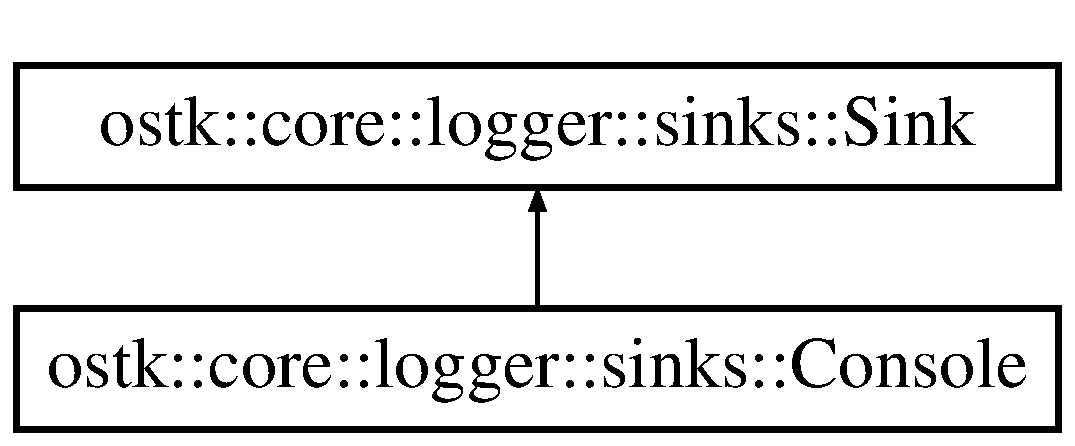
\includegraphics[height=2.000000cm]{classostk_1_1core_1_1logger_1_1sinks_1_1_console}
\end{center}
\end{figure}
\subsection*{Public Types}
\begin{DoxyCompactItemize}
\item 
enum \hyperlink{classostk_1_1core_1_1logger_1_1sinks_1_1_console_abfacace5be69257cad68f802040c050b}{Color} \{ \newline
\hyperlink{classostk_1_1core_1_1logger_1_1sinks_1_1_console_abfacace5be69257cad68f802040c050bae90dfb84e30edf611e326eeb04d680de}{Color\+::\+Black}, 
\hyperlink{classostk_1_1core_1_1logger_1_1sinks_1_1_console_abfacace5be69257cad68f802040c050baee38e4d5dd68c4e440825018d549cb47}{Color\+::\+Red}, 
\hyperlink{classostk_1_1core_1_1logger_1_1sinks_1_1_console_abfacace5be69257cad68f802040c050bad382816a3cbeed082c9e216e7392eed1}{Color\+::\+Green}, 
\hyperlink{classostk_1_1core_1_1logger_1_1sinks_1_1_console_abfacace5be69257cad68f802040c050ba51e6cd92b6c45f9affdc158ecca2b8b8}{Color\+::\+Yellow}, 
\newline
\hyperlink{classostk_1_1core_1_1logger_1_1sinks_1_1_console_abfacace5be69257cad68f802040c050ba9594eec95be70e7b1710f730fdda33d9}{Color\+::\+Blue}, 
\hyperlink{classostk_1_1core_1_1logger_1_1sinks_1_1_console_abfacace5be69257cad68f802040c050bab91cc2c1416fcca942b61c7ac5b1a9ac}{Color\+::\+Magenta}, 
\hyperlink{classostk_1_1core_1_1logger_1_1sinks_1_1_console_abfacace5be69257cad68f802040c050ba023c239d2f2538f140a20e72c7b73f20}{Color\+::\+Cyan}, 
\hyperlink{classostk_1_1core_1_1logger_1_1sinks_1_1_console_abfacace5be69257cad68f802040c050bafb55202637692de4a494e9ade4cff2dd}{Color\+::\+Light\+Gray}, 
\newline
\hyperlink{classostk_1_1core_1_1logger_1_1sinks_1_1_console_abfacace5be69257cad68f802040c050ba91e93fc984985226ad4d319a4e4134ab}{Color\+::\+Dark\+Gray}, 
\hyperlink{classostk_1_1core_1_1logger_1_1sinks_1_1_console_abfacace5be69257cad68f802040c050baf9a96fb667261a141d10021a66d6ad0f}{Color\+::\+Light\+Red}, 
\hyperlink{classostk_1_1core_1_1logger_1_1sinks_1_1_console_abfacace5be69257cad68f802040c050ba7a6a38bec67cbc2a39ce22f34e4ed8e2}{Color\+::\+Light\+Green}, 
\hyperlink{classostk_1_1core_1_1logger_1_1sinks_1_1_console_abfacace5be69257cad68f802040c050bafaf948b65bda38f44b17d156177d1728}{Color\+::\+Light\+Yellow}, 
\newline
\hyperlink{classostk_1_1core_1_1logger_1_1sinks_1_1_console_abfacace5be69257cad68f802040c050ba4d7ff7393a484a7b9ed2e381f5cdeaf7}{Color\+::\+Light\+Blue}, 
\hyperlink{classostk_1_1core_1_1logger_1_1sinks_1_1_console_abfacace5be69257cad68f802040c050baf1ec64ef9f82e9fb86b094f8b548f9f1}{Color\+::\+Light\+Magenta}, 
\hyperlink{classostk_1_1core_1_1logger_1_1sinks_1_1_console_abfacace5be69257cad68f802040c050bac37b5ce4ba80a097d82726ae74d34b13}{Color\+::\+Light\+Cyan}, 
\hyperlink{classostk_1_1core_1_1logger_1_1sinks_1_1_console_abfacace5be69257cad68f802040c050ba25a81701fbfa4a1efdf660a950c1d006}{Color\+::\+White}
 \}
\end{DoxyCompactItemize}
\subsection*{Public Member Functions}
\begin{DoxyCompactItemize}
\item 
\hyperlink{classostk_1_1core_1_1logger_1_1sinks_1_1_console_a4ce5bd08c48c3cd4cd9a89108bb116bc}{Console} (const \hyperlink{namespaceostk_1_1core_1_1logger_a52d02954e094391f067befffe7f3cae9}{Severity} \&a\+Severity)
\item 
\hyperlink{classostk_1_1core_1_1logger_1_1sinks_1_1_console_ad92c49ce281244cbbe4465027fbfa8a2}{Console} (const \hyperlink{classostk_1_1core_1_1logger_1_1sinks_1_1_console}{Console} \&a\+Console)
\item 
virtual \hyperlink{classostk_1_1core_1_1logger_1_1sinks_1_1_console_a465348da7ec4f1aa132ae7b976a23f45}{$\sim$\+Console} () override
\item 
virtual \hyperlink{classostk_1_1core_1_1logger_1_1sinks_1_1_console}{Console} $\ast$ \hyperlink{classostk_1_1core_1_1logger_1_1sinks_1_1_console_ab906fb3918a362c527489091e006d521}{clone} () const override
\item 
virtual void \hyperlink{classostk_1_1core_1_1logger_1_1sinks_1_1_console_a684825bbab717a14f9c83712c054d1d9}{enable} () override
\item 
virtual void \hyperlink{classostk_1_1core_1_1logger_1_1sinks_1_1_console_a5872f5826955ff7f6371bce6ea320253}{disable} () override
\end{DoxyCompactItemize}
\subsection*{Static Public Member Functions}
\begin{DoxyCompactItemize}
\item 
static \hyperlink{classostk_1_1core_1_1types_1_1_string}{String} \hyperlink{classostk_1_1core_1_1logger_1_1sinks_1_1_console_a135245244645e842ba7388445d03b16d}{Colorize\+Message} (const \hyperlink{classostk_1_1core_1_1types_1_1_string}{String} \&a\+Message, const \hyperlink{classostk_1_1core_1_1logger_1_1sinks_1_1_console_abfacace5be69257cad68f802040c050b}{Console\+::\+Color} \&a\+Color)
\end{DoxyCompactItemize}
\subsection*{Friends}
\begin{DoxyCompactItemize}
\item 
class \hyperlink{classostk_1_1core_1_1logger_1_1sinks_1_1_console_aeda242f6bb74cf8f4003eb67666e9118}{Console\+::\+Impl}
\end{DoxyCompactItemize}
\subsection*{Additional Inherited Members}


\subsection{Detailed Description}
Log console sink. 

\subsection{Member Enumeration Documentation}
\mbox{\Hypertarget{classostk_1_1core_1_1logger_1_1sinks_1_1_console_abfacace5be69257cad68f802040c050b}\label{classostk_1_1core_1_1logger_1_1sinks_1_1_console_abfacace5be69257cad68f802040c050b}} 
\index{ostk\+::core\+::logger\+::sinks\+::\+Console@{ostk\+::core\+::logger\+::sinks\+::\+Console}!Color@{Color}}
\index{Color@{Color}!ostk\+::core\+::logger\+::sinks\+::\+Console@{ostk\+::core\+::logger\+::sinks\+::\+Console}}
\subsubsection{\texorpdfstring{Color}{Color}}
{\footnotesize\ttfamily enum \hyperlink{classostk_1_1core_1_1logger_1_1sinks_1_1_console_abfacace5be69257cad68f802040c050b}{ostk\+::core\+::logger\+::sinks\+::\+Console\+::\+Color}\hspace{0.3cm}{\ttfamily [strong]}}

\begin{DoxyEnumFields}{Enumerator}
\raisebox{\heightof{T}}[0pt][0pt]{\index{Black@{Black}!ostk\+::core\+::logger\+::sinks\+::\+Console@{ostk\+::core\+::logger\+::sinks\+::\+Console}}\index{ostk\+::core\+::logger\+::sinks\+::\+Console@{ostk\+::core\+::logger\+::sinks\+::\+Console}!Black@{Black}}}\mbox{\Hypertarget{classostk_1_1core_1_1logger_1_1sinks_1_1_console_abfacace5be69257cad68f802040c050bae90dfb84e30edf611e326eeb04d680de}\label{classostk_1_1core_1_1logger_1_1sinks_1_1_console_abfacace5be69257cad68f802040c050bae90dfb84e30edf611e326eeb04d680de}} 
Black&\\
\hline

\raisebox{\heightof{T}}[0pt][0pt]{\index{Red@{Red}!ostk\+::core\+::logger\+::sinks\+::\+Console@{ostk\+::core\+::logger\+::sinks\+::\+Console}}\index{ostk\+::core\+::logger\+::sinks\+::\+Console@{ostk\+::core\+::logger\+::sinks\+::\+Console}!Red@{Red}}}\mbox{\Hypertarget{classostk_1_1core_1_1logger_1_1sinks_1_1_console_abfacace5be69257cad68f802040c050baee38e4d5dd68c4e440825018d549cb47}\label{classostk_1_1core_1_1logger_1_1sinks_1_1_console_abfacace5be69257cad68f802040c050baee38e4d5dd68c4e440825018d549cb47}} 
Red&\\
\hline

\raisebox{\heightof{T}}[0pt][0pt]{\index{Green@{Green}!ostk\+::core\+::logger\+::sinks\+::\+Console@{ostk\+::core\+::logger\+::sinks\+::\+Console}}\index{ostk\+::core\+::logger\+::sinks\+::\+Console@{ostk\+::core\+::logger\+::sinks\+::\+Console}!Green@{Green}}}\mbox{\Hypertarget{classostk_1_1core_1_1logger_1_1sinks_1_1_console_abfacace5be69257cad68f802040c050bad382816a3cbeed082c9e216e7392eed1}\label{classostk_1_1core_1_1logger_1_1sinks_1_1_console_abfacace5be69257cad68f802040c050bad382816a3cbeed082c9e216e7392eed1}} 
Green&\\
\hline

\raisebox{\heightof{T}}[0pt][0pt]{\index{Yellow@{Yellow}!ostk\+::core\+::logger\+::sinks\+::\+Console@{ostk\+::core\+::logger\+::sinks\+::\+Console}}\index{ostk\+::core\+::logger\+::sinks\+::\+Console@{ostk\+::core\+::logger\+::sinks\+::\+Console}!Yellow@{Yellow}}}\mbox{\Hypertarget{classostk_1_1core_1_1logger_1_1sinks_1_1_console_abfacace5be69257cad68f802040c050ba51e6cd92b6c45f9affdc158ecca2b8b8}\label{classostk_1_1core_1_1logger_1_1sinks_1_1_console_abfacace5be69257cad68f802040c050ba51e6cd92b6c45f9affdc158ecca2b8b8}} 
Yellow&\\
\hline

\raisebox{\heightof{T}}[0pt][0pt]{\index{Blue@{Blue}!ostk\+::core\+::logger\+::sinks\+::\+Console@{ostk\+::core\+::logger\+::sinks\+::\+Console}}\index{ostk\+::core\+::logger\+::sinks\+::\+Console@{ostk\+::core\+::logger\+::sinks\+::\+Console}!Blue@{Blue}}}\mbox{\Hypertarget{classostk_1_1core_1_1logger_1_1sinks_1_1_console_abfacace5be69257cad68f802040c050ba9594eec95be70e7b1710f730fdda33d9}\label{classostk_1_1core_1_1logger_1_1sinks_1_1_console_abfacace5be69257cad68f802040c050ba9594eec95be70e7b1710f730fdda33d9}} 
Blue&\\
\hline

\raisebox{\heightof{T}}[0pt][0pt]{\index{Magenta@{Magenta}!ostk\+::core\+::logger\+::sinks\+::\+Console@{ostk\+::core\+::logger\+::sinks\+::\+Console}}\index{ostk\+::core\+::logger\+::sinks\+::\+Console@{ostk\+::core\+::logger\+::sinks\+::\+Console}!Magenta@{Magenta}}}\mbox{\Hypertarget{classostk_1_1core_1_1logger_1_1sinks_1_1_console_abfacace5be69257cad68f802040c050bab91cc2c1416fcca942b61c7ac5b1a9ac}\label{classostk_1_1core_1_1logger_1_1sinks_1_1_console_abfacace5be69257cad68f802040c050bab91cc2c1416fcca942b61c7ac5b1a9ac}} 
Magenta&\\
\hline

\raisebox{\heightof{T}}[0pt][0pt]{\index{Cyan@{Cyan}!ostk\+::core\+::logger\+::sinks\+::\+Console@{ostk\+::core\+::logger\+::sinks\+::\+Console}}\index{ostk\+::core\+::logger\+::sinks\+::\+Console@{ostk\+::core\+::logger\+::sinks\+::\+Console}!Cyan@{Cyan}}}\mbox{\Hypertarget{classostk_1_1core_1_1logger_1_1sinks_1_1_console_abfacace5be69257cad68f802040c050ba023c239d2f2538f140a20e72c7b73f20}\label{classostk_1_1core_1_1logger_1_1sinks_1_1_console_abfacace5be69257cad68f802040c050ba023c239d2f2538f140a20e72c7b73f20}} 
Cyan&\\
\hline

\raisebox{\heightof{T}}[0pt][0pt]{\index{Light\+Gray@{Light\+Gray}!ostk\+::core\+::logger\+::sinks\+::\+Console@{ostk\+::core\+::logger\+::sinks\+::\+Console}}\index{ostk\+::core\+::logger\+::sinks\+::\+Console@{ostk\+::core\+::logger\+::sinks\+::\+Console}!Light\+Gray@{Light\+Gray}}}\mbox{\Hypertarget{classostk_1_1core_1_1logger_1_1sinks_1_1_console_abfacace5be69257cad68f802040c050bafb55202637692de4a494e9ade4cff2dd}\label{classostk_1_1core_1_1logger_1_1sinks_1_1_console_abfacace5be69257cad68f802040c050bafb55202637692de4a494e9ade4cff2dd}} 
Light\+Gray&\\
\hline

\raisebox{\heightof{T}}[0pt][0pt]{\index{Dark\+Gray@{Dark\+Gray}!ostk\+::core\+::logger\+::sinks\+::\+Console@{ostk\+::core\+::logger\+::sinks\+::\+Console}}\index{ostk\+::core\+::logger\+::sinks\+::\+Console@{ostk\+::core\+::logger\+::sinks\+::\+Console}!Dark\+Gray@{Dark\+Gray}}}\mbox{\Hypertarget{classostk_1_1core_1_1logger_1_1sinks_1_1_console_abfacace5be69257cad68f802040c050ba91e93fc984985226ad4d319a4e4134ab}\label{classostk_1_1core_1_1logger_1_1sinks_1_1_console_abfacace5be69257cad68f802040c050ba91e93fc984985226ad4d319a4e4134ab}} 
Dark\+Gray&\\
\hline

\raisebox{\heightof{T}}[0pt][0pt]{\index{Light\+Red@{Light\+Red}!ostk\+::core\+::logger\+::sinks\+::\+Console@{ostk\+::core\+::logger\+::sinks\+::\+Console}}\index{ostk\+::core\+::logger\+::sinks\+::\+Console@{ostk\+::core\+::logger\+::sinks\+::\+Console}!Light\+Red@{Light\+Red}}}\mbox{\Hypertarget{classostk_1_1core_1_1logger_1_1sinks_1_1_console_abfacace5be69257cad68f802040c050baf9a96fb667261a141d10021a66d6ad0f}\label{classostk_1_1core_1_1logger_1_1sinks_1_1_console_abfacace5be69257cad68f802040c050baf9a96fb667261a141d10021a66d6ad0f}} 
Light\+Red&\\
\hline

\raisebox{\heightof{T}}[0pt][0pt]{\index{Light\+Green@{Light\+Green}!ostk\+::core\+::logger\+::sinks\+::\+Console@{ostk\+::core\+::logger\+::sinks\+::\+Console}}\index{ostk\+::core\+::logger\+::sinks\+::\+Console@{ostk\+::core\+::logger\+::sinks\+::\+Console}!Light\+Green@{Light\+Green}}}\mbox{\Hypertarget{classostk_1_1core_1_1logger_1_1sinks_1_1_console_abfacace5be69257cad68f802040c050ba7a6a38bec67cbc2a39ce22f34e4ed8e2}\label{classostk_1_1core_1_1logger_1_1sinks_1_1_console_abfacace5be69257cad68f802040c050ba7a6a38bec67cbc2a39ce22f34e4ed8e2}} 
Light\+Green&\\
\hline

\raisebox{\heightof{T}}[0pt][0pt]{\index{Light\+Yellow@{Light\+Yellow}!ostk\+::core\+::logger\+::sinks\+::\+Console@{ostk\+::core\+::logger\+::sinks\+::\+Console}}\index{ostk\+::core\+::logger\+::sinks\+::\+Console@{ostk\+::core\+::logger\+::sinks\+::\+Console}!Light\+Yellow@{Light\+Yellow}}}\mbox{\Hypertarget{classostk_1_1core_1_1logger_1_1sinks_1_1_console_abfacace5be69257cad68f802040c050bafaf948b65bda38f44b17d156177d1728}\label{classostk_1_1core_1_1logger_1_1sinks_1_1_console_abfacace5be69257cad68f802040c050bafaf948b65bda38f44b17d156177d1728}} 
Light\+Yellow&\\
\hline

\raisebox{\heightof{T}}[0pt][0pt]{\index{Light\+Blue@{Light\+Blue}!ostk\+::core\+::logger\+::sinks\+::\+Console@{ostk\+::core\+::logger\+::sinks\+::\+Console}}\index{ostk\+::core\+::logger\+::sinks\+::\+Console@{ostk\+::core\+::logger\+::sinks\+::\+Console}!Light\+Blue@{Light\+Blue}}}\mbox{\Hypertarget{classostk_1_1core_1_1logger_1_1sinks_1_1_console_abfacace5be69257cad68f802040c050ba4d7ff7393a484a7b9ed2e381f5cdeaf7}\label{classostk_1_1core_1_1logger_1_1sinks_1_1_console_abfacace5be69257cad68f802040c050ba4d7ff7393a484a7b9ed2e381f5cdeaf7}} 
Light\+Blue&\\
\hline

\raisebox{\heightof{T}}[0pt][0pt]{\index{Light\+Magenta@{Light\+Magenta}!ostk\+::core\+::logger\+::sinks\+::\+Console@{ostk\+::core\+::logger\+::sinks\+::\+Console}}\index{ostk\+::core\+::logger\+::sinks\+::\+Console@{ostk\+::core\+::logger\+::sinks\+::\+Console}!Light\+Magenta@{Light\+Magenta}}}\mbox{\Hypertarget{classostk_1_1core_1_1logger_1_1sinks_1_1_console_abfacace5be69257cad68f802040c050baf1ec64ef9f82e9fb86b094f8b548f9f1}\label{classostk_1_1core_1_1logger_1_1sinks_1_1_console_abfacace5be69257cad68f802040c050baf1ec64ef9f82e9fb86b094f8b548f9f1}} 
Light\+Magenta&\\
\hline

\raisebox{\heightof{T}}[0pt][0pt]{\index{Light\+Cyan@{Light\+Cyan}!ostk\+::core\+::logger\+::sinks\+::\+Console@{ostk\+::core\+::logger\+::sinks\+::\+Console}}\index{ostk\+::core\+::logger\+::sinks\+::\+Console@{ostk\+::core\+::logger\+::sinks\+::\+Console}!Light\+Cyan@{Light\+Cyan}}}\mbox{\Hypertarget{classostk_1_1core_1_1logger_1_1sinks_1_1_console_abfacace5be69257cad68f802040c050bac37b5ce4ba80a097d82726ae74d34b13}\label{classostk_1_1core_1_1logger_1_1sinks_1_1_console_abfacace5be69257cad68f802040c050bac37b5ce4ba80a097d82726ae74d34b13}} 
Light\+Cyan&\\
\hline

\raisebox{\heightof{T}}[0pt][0pt]{\index{White@{White}!ostk\+::core\+::logger\+::sinks\+::\+Console@{ostk\+::core\+::logger\+::sinks\+::\+Console}}\index{ostk\+::core\+::logger\+::sinks\+::\+Console@{ostk\+::core\+::logger\+::sinks\+::\+Console}!White@{White}}}\mbox{\Hypertarget{classostk_1_1core_1_1logger_1_1sinks_1_1_console_abfacace5be69257cad68f802040c050ba25a81701fbfa4a1efdf660a950c1d006}\label{classostk_1_1core_1_1logger_1_1sinks_1_1_console_abfacace5be69257cad68f802040c050ba25a81701fbfa4a1efdf660a950c1d006}} 
White&\\
\hline

\end{DoxyEnumFields}


\subsection{Constructor \& Destructor Documentation}
\mbox{\Hypertarget{classostk_1_1core_1_1logger_1_1sinks_1_1_console_a4ce5bd08c48c3cd4cd9a89108bb116bc}\label{classostk_1_1core_1_1logger_1_1sinks_1_1_console_a4ce5bd08c48c3cd4cd9a89108bb116bc}} 
\index{ostk\+::core\+::logger\+::sinks\+::\+Console@{ostk\+::core\+::logger\+::sinks\+::\+Console}!Console@{Console}}
\index{Console@{Console}!ostk\+::core\+::logger\+::sinks\+::\+Console@{ostk\+::core\+::logger\+::sinks\+::\+Console}}
\subsubsection{\texorpdfstring{Console()}{Console()}\hspace{0.1cm}{\footnotesize\ttfamily [1/2]}}
{\footnotesize\ttfamily ostk\+::core\+::logger\+::sinks\+::\+Console\+::\+Console (\begin{DoxyParamCaption}\item[{const \hyperlink{namespaceostk_1_1core_1_1logger_a52d02954e094391f067befffe7f3cae9}{Severity} \&}]{a\+Severity }\end{DoxyParamCaption})}

\mbox{\Hypertarget{classostk_1_1core_1_1logger_1_1sinks_1_1_console_ad92c49ce281244cbbe4465027fbfa8a2}\label{classostk_1_1core_1_1logger_1_1sinks_1_1_console_ad92c49ce281244cbbe4465027fbfa8a2}} 
\index{ostk\+::core\+::logger\+::sinks\+::\+Console@{ostk\+::core\+::logger\+::sinks\+::\+Console}!Console@{Console}}
\index{Console@{Console}!ostk\+::core\+::logger\+::sinks\+::\+Console@{ostk\+::core\+::logger\+::sinks\+::\+Console}}
\subsubsection{\texorpdfstring{Console()}{Console()}\hspace{0.1cm}{\footnotesize\ttfamily [2/2]}}
{\footnotesize\ttfamily ostk\+::core\+::logger\+::sinks\+::\+Console\+::\+Console (\begin{DoxyParamCaption}\item[{const \hyperlink{classostk_1_1core_1_1logger_1_1sinks_1_1_console}{Console} \&}]{a\+Console }\end{DoxyParamCaption})}

\mbox{\Hypertarget{classostk_1_1core_1_1logger_1_1sinks_1_1_console_a465348da7ec4f1aa132ae7b976a23f45}\label{classostk_1_1core_1_1logger_1_1sinks_1_1_console_a465348da7ec4f1aa132ae7b976a23f45}} 
\index{ostk\+::core\+::logger\+::sinks\+::\+Console@{ostk\+::core\+::logger\+::sinks\+::\+Console}!````~Console@{$\sim$\+Console}}
\index{````~Console@{$\sim$\+Console}!ostk\+::core\+::logger\+::sinks\+::\+Console@{ostk\+::core\+::logger\+::sinks\+::\+Console}}
\subsubsection{\texorpdfstring{$\sim$\+Console()}{~Console()}}
{\footnotesize\ttfamily virtual ostk\+::core\+::logger\+::sinks\+::\+Console\+::$\sim$\+Console (\begin{DoxyParamCaption}{ }\end{DoxyParamCaption})\hspace{0.3cm}{\ttfamily [override]}, {\ttfamily [virtual]}}



\subsection{Member Function Documentation}
\mbox{\Hypertarget{classostk_1_1core_1_1logger_1_1sinks_1_1_console_ab906fb3918a362c527489091e006d521}\label{classostk_1_1core_1_1logger_1_1sinks_1_1_console_ab906fb3918a362c527489091e006d521}} 
\index{ostk\+::core\+::logger\+::sinks\+::\+Console@{ostk\+::core\+::logger\+::sinks\+::\+Console}!clone@{clone}}
\index{clone@{clone}!ostk\+::core\+::logger\+::sinks\+::\+Console@{ostk\+::core\+::logger\+::sinks\+::\+Console}}
\subsubsection{\texorpdfstring{clone()}{clone()}}
{\footnotesize\ttfamily virtual \hyperlink{classostk_1_1core_1_1logger_1_1sinks_1_1_console}{Console}$\ast$ ostk\+::core\+::logger\+::sinks\+::\+Console\+::clone (\begin{DoxyParamCaption}{ }\end{DoxyParamCaption}) const\hspace{0.3cm}{\ttfamily [override]}, {\ttfamily [virtual]}}



Implements \hyperlink{classostk_1_1core_1_1logger_1_1sinks_1_1_sink_a0e6b41f9b4626b5229370f71bd27be32}{ostk\+::core\+::logger\+::sinks\+::\+Sink}.

\mbox{\Hypertarget{classostk_1_1core_1_1logger_1_1sinks_1_1_console_a135245244645e842ba7388445d03b16d}\label{classostk_1_1core_1_1logger_1_1sinks_1_1_console_a135245244645e842ba7388445d03b16d}} 
\index{ostk\+::core\+::logger\+::sinks\+::\+Console@{ostk\+::core\+::logger\+::sinks\+::\+Console}!Colorize\+Message@{Colorize\+Message}}
\index{Colorize\+Message@{Colorize\+Message}!ostk\+::core\+::logger\+::sinks\+::\+Console@{ostk\+::core\+::logger\+::sinks\+::\+Console}}
\subsubsection{\texorpdfstring{Colorize\+Message()}{ColorizeMessage()}}
{\footnotesize\ttfamily static \hyperlink{classostk_1_1core_1_1types_1_1_string}{String} ostk\+::core\+::logger\+::sinks\+::\+Console\+::\+Colorize\+Message (\begin{DoxyParamCaption}\item[{const \hyperlink{classostk_1_1core_1_1types_1_1_string}{String} \&}]{a\+Message,  }\item[{const \hyperlink{classostk_1_1core_1_1logger_1_1sinks_1_1_console_abfacace5be69257cad68f802040c050b}{Console\+::\+Color} \&}]{a\+Color }\end{DoxyParamCaption})\hspace{0.3cm}{\ttfamily [static]}}

\mbox{\Hypertarget{classostk_1_1core_1_1logger_1_1sinks_1_1_console_a5872f5826955ff7f6371bce6ea320253}\label{classostk_1_1core_1_1logger_1_1sinks_1_1_console_a5872f5826955ff7f6371bce6ea320253}} 
\index{ostk\+::core\+::logger\+::sinks\+::\+Console@{ostk\+::core\+::logger\+::sinks\+::\+Console}!disable@{disable}}
\index{disable@{disable}!ostk\+::core\+::logger\+::sinks\+::\+Console@{ostk\+::core\+::logger\+::sinks\+::\+Console}}
\subsubsection{\texorpdfstring{disable()}{disable()}}
{\footnotesize\ttfamily virtual void ostk\+::core\+::logger\+::sinks\+::\+Console\+::disable (\begin{DoxyParamCaption}{ }\end{DoxyParamCaption})\hspace{0.3cm}{\ttfamily [override]}, {\ttfamily [virtual]}}



Implements \hyperlink{classostk_1_1core_1_1logger_1_1sinks_1_1_sink_a3e347ffee80e3c2ee50ff0edf9265115}{ostk\+::core\+::logger\+::sinks\+::\+Sink}.

\mbox{\Hypertarget{classostk_1_1core_1_1logger_1_1sinks_1_1_console_a684825bbab717a14f9c83712c054d1d9}\label{classostk_1_1core_1_1logger_1_1sinks_1_1_console_a684825bbab717a14f9c83712c054d1d9}} 
\index{ostk\+::core\+::logger\+::sinks\+::\+Console@{ostk\+::core\+::logger\+::sinks\+::\+Console}!enable@{enable}}
\index{enable@{enable}!ostk\+::core\+::logger\+::sinks\+::\+Console@{ostk\+::core\+::logger\+::sinks\+::\+Console}}
\subsubsection{\texorpdfstring{enable()}{enable()}}
{\footnotesize\ttfamily virtual void ostk\+::core\+::logger\+::sinks\+::\+Console\+::enable (\begin{DoxyParamCaption}{ }\end{DoxyParamCaption})\hspace{0.3cm}{\ttfamily [override]}, {\ttfamily [virtual]}}



Implements \hyperlink{classostk_1_1core_1_1logger_1_1sinks_1_1_sink_a355c81571a4a34bb162c1dc5fe631c89}{ostk\+::core\+::logger\+::sinks\+::\+Sink}.



\subsection{Friends And Related Function Documentation}
\mbox{\Hypertarget{classostk_1_1core_1_1logger_1_1sinks_1_1_console_aeda242f6bb74cf8f4003eb67666e9118}\label{classostk_1_1core_1_1logger_1_1sinks_1_1_console_aeda242f6bb74cf8f4003eb67666e9118}} 
\index{ostk\+::core\+::logger\+::sinks\+::\+Console@{ostk\+::core\+::logger\+::sinks\+::\+Console}!Console\+::\+Impl@{Console\+::\+Impl}}
\index{Console\+::\+Impl@{Console\+::\+Impl}!ostk\+::core\+::logger\+::sinks\+::\+Console@{ostk\+::core\+::logger\+::sinks\+::\+Console}}
\subsubsection{\texorpdfstring{Console\+::\+Impl}{Console::Impl}}
{\footnotesize\ttfamily friend class Console\+::\+Impl\hspace{0.3cm}{\ttfamily [friend]}}



The documentation for this class was generated from the following file\+:\begin{DoxyCompactItemize}
\item 
include/\+Open\+Space\+Toolkit/\+Core/\+Logger/\+Sinks/\hyperlink{_console_8hpp}{Console.\+hpp}\end{DoxyCompactItemize}

\hypertarget{classostk_1_1core_1_1ctnr_1_1_dictionary_1_1_const_iterator}{}\section{ostk\+:\+:core\+:\+:ctnr\+:\+:Dictionary\+:\+:Const\+Iterator Class Reference}
\label{classostk_1_1core_1_1ctnr_1_1_dictionary_1_1_const_iterator}\index{ostk\+::core\+::ctnr\+::\+Dictionary\+::\+Const\+Iterator@{ostk\+::core\+::ctnr\+::\+Dictionary\+::\+Const\+Iterator}}


{\ttfamily \#include $<$Dictionary.\+hpp$>$}

\subsection*{Public Types}
\begin{DoxyCompactItemize}
\item 
typedef \hyperlink{namespaceostk_1_1core_1_1ctnr_a13ac23065e75eb425f38bfca4d0c6b38}{Ordered\+Map}$<$ \hyperlink{classostk_1_1core_1_1ctnr_1_1_dictionary_aa3b171525039535f342d271d27f90407}{Dictionary\+::\+Key}, \hyperlink{classostk_1_1core_1_1ctnr_1_1_dictionary_ace6ab82268031e972455affca8730c9c}{Dictionary\+::\+Value} $>$\+::const\+\_\+iterator \hyperlink{classostk_1_1core_1_1ctnr_1_1_dictionary_1_1_const_iterator_a7c7a0e5a0a15da39cbb2115306fdef4c}{Map\+Const\+Iterator}
\end{DoxyCompactItemize}
\subsection*{Public Member Functions}
\begin{DoxyCompactItemize}
\item 
\hyperlink{classostk_1_1core_1_1ctnr_1_1_dictionary_1_1_const_iterator_a308d67ac775d7f6e024546a68bdd2fb4}{Const\+Iterator} ()
\item 
\hyperlink{classostk_1_1core_1_1ctnr_1_1_dictionary_1_1_const_iterator_afcd7ded3d55a228787ff87831e95dea7}{Const\+Iterator} (const \hyperlink{classostk_1_1core_1_1ctnr_1_1_dictionary_1_1_const_iterator_a7c7a0e5a0a15da39cbb2115306fdef4c}{Const\+Iterator\+::\+Map\+Const\+Iterator} \&an\+Ordered\+Map\+It)
\item 
\hyperlink{classostk_1_1core_1_1ctnr_1_1_dictionary_1_1_const_iterator_a174b8bc8d3945878fdb33c160a9892ac}{Const\+Iterator} (const \hyperlink{classostk_1_1core_1_1ctnr_1_1_dictionary_1_1_const_iterator}{Const\+Iterator} \&a\+Const\+Iterator)
\item 
\hyperlink{classostk_1_1core_1_1ctnr_1_1_dictionary_1_1_const_iterator_a37d0c7da312c753460f0a7358f94082e}{Const\+Iterator} (const \hyperlink{classostk_1_1core_1_1ctnr_1_1_dictionary_1_1_iterator}{Iterator} \&an\+Iterator)
\item 
\hyperlink{classostk_1_1core_1_1ctnr_1_1_dictionary_1_1_const_iterator}{Const\+Iterator} \& \hyperlink{classostk_1_1core_1_1ctnr_1_1_dictionary_1_1_const_iterator_aa775f33410700e7323e76696805664c6}{operator=} (const \hyperlink{classostk_1_1core_1_1ctnr_1_1_dictionary_1_1_const_iterator}{Const\+Iterator} \&a\+Const\+Iterator)
\item 
bool \hyperlink{classostk_1_1core_1_1ctnr_1_1_dictionary_1_1_const_iterator_a6df9476c601d51a28a4a4b8c5d8ea0d0}{operator==} (const \hyperlink{classostk_1_1core_1_1ctnr_1_1_dictionary_1_1_const_iterator}{Const\+Iterator} \&a\+Const\+Iterator) const
\item 
bool \hyperlink{classostk_1_1core_1_1ctnr_1_1_dictionary_1_1_const_iterator_aecc04d372953754c18cba9c932514cb0}{operator!=} (const \hyperlink{classostk_1_1core_1_1ctnr_1_1_dictionary_1_1_const_iterator}{Const\+Iterator} \&a\+Const\+Iterator) const
\item 
const \hyperlink{classostk_1_1core_1_1ctnr_1_1_dictionary_1_1_const_iterator}{Const\+Iterator} \& \hyperlink{classostk_1_1core_1_1ctnr_1_1_dictionary_1_1_const_iterator_a184e1799637eb915d1a05acc962faaa4}{operator$\ast$} () const
\item 
const \hyperlink{classostk_1_1core_1_1ctnr_1_1_dictionary_1_1_const_iterator}{Const\+Iterator} $\ast$ \hyperlink{classostk_1_1core_1_1ctnr_1_1_dictionary_1_1_const_iterator_a18803913871b7f6c7425f9c3ce6c8162}{operator-\/$>$} () const
\item 
const \hyperlink{classostk_1_1core_1_1ctnr_1_1_dictionary_ace6ab82268031e972455affca8730c9c}{Dictionary\+::\+Value} \& \hyperlink{classostk_1_1core_1_1ctnr_1_1_dictionary_1_1_const_iterator_ae360562b0726a4c847d17530e6bcc7ee}{operator\mbox{[}$\,$\mbox{]}} (const \hyperlink{classostk_1_1core_1_1ctnr_1_1_dictionary_aa3b171525039535f342d271d27f90407}{Dictionary\+::\+Key} \&a\+Key) const
\item 
\hyperlink{classostk_1_1core_1_1ctnr_1_1_dictionary_1_1_const_iterator}{Const\+Iterator} \& \hyperlink{classostk_1_1core_1_1ctnr_1_1_dictionary_1_1_const_iterator_a987d4aa2a55050dd7aec162421fa532c}{operator++} ()
\item 
\hyperlink{classostk_1_1core_1_1ctnr_1_1_dictionary_1_1_const_iterator}{Const\+Iterator} \hyperlink{classostk_1_1core_1_1ctnr_1_1_dictionary_1_1_const_iterator_a0b501d2efbe1cc17de54991c4d289206}{operator++} (int)
\item 
\hyperlink{classostk_1_1core_1_1ctnr_1_1_dictionary_1_1_const_iterator}{Const\+Iterator} \& \hyperlink{classostk_1_1core_1_1ctnr_1_1_dictionary_1_1_const_iterator_a38984ba0816c656601ceddb68f15b1dc}{operator-\/-\/} ()
\item 
\hyperlink{classostk_1_1core_1_1ctnr_1_1_dictionary_1_1_const_iterator}{Const\+Iterator} \hyperlink{classostk_1_1core_1_1ctnr_1_1_dictionary_1_1_const_iterator_aaa90af350d5883a2e665fe8c883ec3f9}{operator-\/-\/} (int)
\item 
const \hyperlink{classostk_1_1core_1_1ctnr_1_1_dictionary_aa3b171525039535f342d271d27f90407}{Dictionary\+::\+Key} \& \hyperlink{classostk_1_1core_1_1ctnr_1_1_dictionary_1_1_const_iterator_a87a5017d24ae56e202e043acfd4c6e7f}{access\+Key} () const
\item 
const \hyperlink{classostk_1_1core_1_1ctnr_1_1_dictionary_ace6ab82268031e972455affca8730c9c}{Dictionary\+::\+Value} \& \hyperlink{classostk_1_1core_1_1ctnr_1_1_dictionary_1_1_const_iterator_a1a756f4365bbae65e5086cffe7d40fba}{access\+Value} () const
\item 
\hyperlink{classostk_1_1core_1_1ctnr_1_1_dictionary_1_1_const_iterator_a7c7a0e5a0a15da39cbb2115306fdef4c}{Const\+Iterator\+::\+Map\+Const\+Iterator} \& \hyperlink{classostk_1_1core_1_1ctnr_1_1_dictionary_1_1_const_iterator_a19fb77d28e387720605247372e9b2b1e}{access\+Map\+Const\+Iterator} ()
\end{DoxyCompactItemize}


\subsection{Member Typedef Documentation}
\mbox{\Hypertarget{classostk_1_1core_1_1ctnr_1_1_dictionary_1_1_const_iterator_a7c7a0e5a0a15da39cbb2115306fdef4c}\label{classostk_1_1core_1_1ctnr_1_1_dictionary_1_1_const_iterator_a7c7a0e5a0a15da39cbb2115306fdef4c}} 
\index{ostk\+::core\+::ctnr\+::\+Dictionary\+::\+Const\+Iterator@{ostk\+::core\+::ctnr\+::\+Dictionary\+::\+Const\+Iterator}!Map\+Const\+Iterator@{Map\+Const\+Iterator}}
\index{Map\+Const\+Iterator@{Map\+Const\+Iterator}!ostk\+::core\+::ctnr\+::\+Dictionary\+::\+Const\+Iterator@{ostk\+::core\+::ctnr\+::\+Dictionary\+::\+Const\+Iterator}}
\subsubsection{\texorpdfstring{Map\+Const\+Iterator}{MapConstIterator}}
{\footnotesize\ttfamily typedef \hyperlink{namespaceostk_1_1core_1_1ctnr_a13ac23065e75eb425f38bfca4d0c6b38}{Ordered\+Map}$<$\hyperlink{classostk_1_1core_1_1ctnr_1_1_dictionary_aa3b171525039535f342d271d27f90407}{Dictionary\+::\+Key}, \hyperlink{classostk_1_1core_1_1ctnr_1_1_dictionary_ace6ab82268031e972455affca8730c9c}{Dictionary\+::\+Value}$>$\+::const\+\_\+iterator \hyperlink{classostk_1_1core_1_1ctnr_1_1_dictionary_1_1_const_iterator_a7c7a0e5a0a15da39cbb2115306fdef4c}{ostk\+::core\+::ctnr\+::\+Dictionary\+::\+Const\+Iterator\+::\+Map\+Const\+Iterator}}



\subsection{Constructor \& Destructor Documentation}
\mbox{\Hypertarget{classostk_1_1core_1_1ctnr_1_1_dictionary_1_1_const_iterator_a308d67ac775d7f6e024546a68bdd2fb4}\label{classostk_1_1core_1_1ctnr_1_1_dictionary_1_1_const_iterator_a308d67ac775d7f6e024546a68bdd2fb4}} 
\index{ostk\+::core\+::ctnr\+::\+Dictionary\+::\+Const\+Iterator@{ostk\+::core\+::ctnr\+::\+Dictionary\+::\+Const\+Iterator}!Const\+Iterator@{Const\+Iterator}}
\index{Const\+Iterator@{Const\+Iterator}!ostk\+::core\+::ctnr\+::\+Dictionary\+::\+Const\+Iterator@{ostk\+::core\+::ctnr\+::\+Dictionary\+::\+Const\+Iterator}}
\subsubsection{\texorpdfstring{Const\+Iterator()}{ConstIterator()}\hspace{0.1cm}{\footnotesize\ttfamily [1/4]}}
{\footnotesize\ttfamily ostk\+::core\+::ctnr\+::\+Dictionary\+::\+Const\+Iterator\+::\+Const\+Iterator (\begin{DoxyParamCaption}{ }\end{DoxyParamCaption})}

\mbox{\Hypertarget{classostk_1_1core_1_1ctnr_1_1_dictionary_1_1_const_iterator_afcd7ded3d55a228787ff87831e95dea7}\label{classostk_1_1core_1_1ctnr_1_1_dictionary_1_1_const_iterator_afcd7ded3d55a228787ff87831e95dea7}} 
\index{ostk\+::core\+::ctnr\+::\+Dictionary\+::\+Const\+Iterator@{ostk\+::core\+::ctnr\+::\+Dictionary\+::\+Const\+Iterator}!Const\+Iterator@{Const\+Iterator}}
\index{Const\+Iterator@{Const\+Iterator}!ostk\+::core\+::ctnr\+::\+Dictionary\+::\+Const\+Iterator@{ostk\+::core\+::ctnr\+::\+Dictionary\+::\+Const\+Iterator}}
\subsubsection{\texorpdfstring{Const\+Iterator()}{ConstIterator()}\hspace{0.1cm}{\footnotesize\ttfamily [2/4]}}
{\footnotesize\ttfamily ostk\+::core\+::ctnr\+::\+Dictionary\+::\+Const\+Iterator\+::\+Const\+Iterator (\begin{DoxyParamCaption}\item[{const \hyperlink{classostk_1_1core_1_1ctnr_1_1_dictionary_1_1_const_iterator_a7c7a0e5a0a15da39cbb2115306fdef4c}{Const\+Iterator\+::\+Map\+Const\+Iterator} \&}]{an\+Ordered\+Map\+It }\end{DoxyParamCaption})}

\mbox{\Hypertarget{classostk_1_1core_1_1ctnr_1_1_dictionary_1_1_const_iterator_a174b8bc8d3945878fdb33c160a9892ac}\label{classostk_1_1core_1_1ctnr_1_1_dictionary_1_1_const_iterator_a174b8bc8d3945878fdb33c160a9892ac}} 
\index{ostk\+::core\+::ctnr\+::\+Dictionary\+::\+Const\+Iterator@{ostk\+::core\+::ctnr\+::\+Dictionary\+::\+Const\+Iterator}!Const\+Iterator@{Const\+Iterator}}
\index{Const\+Iterator@{Const\+Iterator}!ostk\+::core\+::ctnr\+::\+Dictionary\+::\+Const\+Iterator@{ostk\+::core\+::ctnr\+::\+Dictionary\+::\+Const\+Iterator}}
\subsubsection{\texorpdfstring{Const\+Iterator()}{ConstIterator()}\hspace{0.1cm}{\footnotesize\ttfamily [3/4]}}
{\footnotesize\ttfamily ostk\+::core\+::ctnr\+::\+Dictionary\+::\+Const\+Iterator\+::\+Const\+Iterator (\begin{DoxyParamCaption}\item[{const \hyperlink{classostk_1_1core_1_1ctnr_1_1_dictionary_1_1_const_iterator}{Const\+Iterator} \&}]{a\+Const\+Iterator }\end{DoxyParamCaption})}

\mbox{\Hypertarget{classostk_1_1core_1_1ctnr_1_1_dictionary_1_1_const_iterator_a37d0c7da312c753460f0a7358f94082e}\label{classostk_1_1core_1_1ctnr_1_1_dictionary_1_1_const_iterator_a37d0c7da312c753460f0a7358f94082e}} 
\index{ostk\+::core\+::ctnr\+::\+Dictionary\+::\+Const\+Iterator@{ostk\+::core\+::ctnr\+::\+Dictionary\+::\+Const\+Iterator}!Const\+Iterator@{Const\+Iterator}}
\index{Const\+Iterator@{Const\+Iterator}!ostk\+::core\+::ctnr\+::\+Dictionary\+::\+Const\+Iterator@{ostk\+::core\+::ctnr\+::\+Dictionary\+::\+Const\+Iterator}}
\subsubsection{\texorpdfstring{Const\+Iterator()}{ConstIterator()}\hspace{0.1cm}{\footnotesize\ttfamily [4/4]}}
{\footnotesize\ttfamily ostk\+::core\+::ctnr\+::\+Dictionary\+::\+Const\+Iterator\+::\+Const\+Iterator (\begin{DoxyParamCaption}\item[{const \hyperlink{classostk_1_1core_1_1ctnr_1_1_dictionary_1_1_iterator}{Iterator} \&}]{an\+Iterator }\end{DoxyParamCaption})}



\subsection{Member Function Documentation}
\mbox{\Hypertarget{classostk_1_1core_1_1ctnr_1_1_dictionary_1_1_const_iterator_a87a5017d24ae56e202e043acfd4c6e7f}\label{classostk_1_1core_1_1ctnr_1_1_dictionary_1_1_const_iterator_a87a5017d24ae56e202e043acfd4c6e7f}} 
\index{ostk\+::core\+::ctnr\+::\+Dictionary\+::\+Const\+Iterator@{ostk\+::core\+::ctnr\+::\+Dictionary\+::\+Const\+Iterator}!access\+Key@{access\+Key}}
\index{access\+Key@{access\+Key}!ostk\+::core\+::ctnr\+::\+Dictionary\+::\+Const\+Iterator@{ostk\+::core\+::ctnr\+::\+Dictionary\+::\+Const\+Iterator}}
\subsubsection{\texorpdfstring{access\+Key()}{accessKey()}}
{\footnotesize\ttfamily const \hyperlink{classostk_1_1core_1_1ctnr_1_1_dictionary_aa3b171525039535f342d271d27f90407}{Dictionary\+::\+Key} \& ostk\+::core\+::ctnr\+::\+Dictionary\+::\+Const\+Iterator\+::access\+Key (\begin{DoxyParamCaption}{ }\end{DoxyParamCaption}) const}

\mbox{\Hypertarget{classostk_1_1core_1_1ctnr_1_1_dictionary_1_1_const_iterator_a19fb77d28e387720605247372e9b2b1e}\label{classostk_1_1core_1_1ctnr_1_1_dictionary_1_1_const_iterator_a19fb77d28e387720605247372e9b2b1e}} 
\index{ostk\+::core\+::ctnr\+::\+Dictionary\+::\+Const\+Iterator@{ostk\+::core\+::ctnr\+::\+Dictionary\+::\+Const\+Iterator}!access\+Map\+Const\+Iterator@{access\+Map\+Const\+Iterator}}
\index{access\+Map\+Const\+Iterator@{access\+Map\+Const\+Iterator}!ostk\+::core\+::ctnr\+::\+Dictionary\+::\+Const\+Iterator@{ostk\+::core\+::ctnr\+::\+Dictionary\+::\+Const\+Iterator}}
\subsubsection{\texorpdfstring{access\+Map\+Const\+Iterator()}{accessMapConstIterator()}}
{\footnotesize\ttfamily \hyperlink{classostk_1_1core_1_1ctnr_1_1_dictionary_1_1_const_iterator_a7c7a0e5a0a15da39cbb2115306fdef4c}{Dictionary\+::\+Const\+Iterator\+::\+Map\+Const\+Iterator} \& ostk\+::core\+::ctnr\+::\+Dictionary\+::\+Const\+Iterator\+::access\+Map\+Const\+Iterator (\begin{DoxyParamCaption}{ }\end{DoxyParamCaption})}

\mbox{\Hypertarget{classostk_1_1core_1_1ctnr_1_1_dictionary_1_1_const_iterator_a1a756f4365bbae65e5086cffe7d40fba}\label{classostk_1_1core_1_1ctnr_1_1_dictionary_1_1_const_iterator_a1a756f4365bbae65e5086cffe7d40fba}} 
\index{ostk\+::core\+::ctnr\+::\+Dictionary\+::\+Const\+Iterator@{ostk\+::core\+::ctnr\+::\+Dictionary\+::\+Const\+Iterator}!access\+Value@{access\+Value}}
\index{access\+Value@{access\+Value}!ostk\+::core\+::ctnr\+::\+Dictionary\+::\+Const\+Iterator@{ostk\+::core\+::ctnr\+::\+Dictionary\+::\+Const\+Iterator}}
\subsubsection{\texorpdfstring{access\+Value()}{accessValue()}}
{\footnotesize\ttfamily const \hyperlink{classostk_1_1core_1_1ctnr_1_1_dictionary_ace6ab82268031e972455affca8730c9c}{Dictionary\+::\+Value} \& ostk\+::core\+::ctnr\+::\+Dictionary\+::\+Const\+Iterator\+::access\+Value (\begin{DoxyParamCaption}{ }\end{DoxyParamCaption}) const}

\mbox{\Hypertarget{classostk_1_1core_1_1ctnr_1_1_dictionary_1_1_const_iterator_aecc04d372953754c18cba9c932514cb0}\label{classostk_1_1core_1_1ctnr_1_1_dictionary_1_1_const_iterator_aecc04d372953754c18cba9c932514cb0}} 
\index{ostk\+::core\+::ctnr\+::\+Dictionary\+::\+Const\+Iterator@{ostk\+::core\+::ctnr\+::\+Dictionary\+::\+Const\+Iterator}!operator"!=@{operator"!=}}
\index{operator"!=@{operator"!=}!ostk\+::core\+::ctnr\+::\+Dictionary\+::\+Const\+Iterator@{ostk\+::core\+::ctnr\+::\+Dictionary\+::\+Const\+Iterator}}
\subsubsection{\texorpdfstring{operator"!=()}{operator!=()}}
{\footnotesize\ttfamily bool ostk\+::core\+::ctnr\+::\+Dictionary\+::\+Const\+Iterator\+::operator!= (\begin{DoxyParamCaption}\item[{const \hyperlink{classostk_1_1core_1_1ctnr_1_1_dictionary_1_1_const_iterator}{Const\+Iterator} \&}]{a\+Const\+Iterator }\end{DoxyParamCaption}) const}

\mbox{\Hypertarget{classostk_1_1core_1_1ctnr_1_1_dictionary_1_1_const_iterator_a184e1799637eb915d1a05acc962faaa4}\label{classostk_1_1core_1_1ctnr_1_1_dictionary_1_1_const_iterator_a184e1799637eb915d1a05acc962faaa4}} 
\index{ostk\+::core\+::ctnr\+::\+Dictionary\+::\+Const\+Iterator@{ostk\+::core\+::ctnr\+::\+Dictionary\+::\+Const\+Iterator}!operator$\ast$@{operator$\ast$}}
\index{operator$\ast$@{operator$\ast$}!ostk\+::core\+::ctnr\+::\+Dictionary\+::\+Const\+Iterator@{ostk\+::core\+::ctnr\+::\+Dictionary\+::\+Const\+Iterator}}
\subsubsection{\texorpdfstring{operator$\ast$()}{operator*()}}
{\footnotesize\ttfamily const \hyperlink{classostk_1_1core_1_1ctnr_1_1_dictionary_1_1_const_iterator}{Dictionary\+::\+Const\+Iterator} \& ostk\+::core\+::ctnr\+::\+Dictionary\+::\+Const\+Iterator\+::operator$\ast$ (\begin{DoxyParamCaption}{ }\end{DoxyParamCaption}) const}

\mbox{\Hypertarget{classostk_1_1core_1_1ctnr_1_1_dictionary_1_1_const_iterator_a987d4aa2a55050dd7aec162421fa532c}\label{classostk_1_1core_1_1ctnr_1_1_dictionary_1_1_const_iterator_a987d4aa2a55050dd7aec162421fa532c}} 
\index{ostk\+::core\+::ctnr\+::\+Dictionary\+::\+Const\+Iterator@{ostk\+::core\+::ctnr\+::\+Dictionary\+::\+Const\+Iterator}!operator++@{operator++}}
\index{operator++@{operator++}!ostk\+::core\+::ctnr\+::\+Dictionary\+::\+Const\+Iterator@{ostk\+::core\+::ctnr\+::\+Dictionary\+::\+Const\+Iterator}}
\subsubsection{\texorpdfstring{operator++()}{operator++()}\hspace{0.1cm}{\footnotesize\ttfamily [1/2]}}
{\footnotesize\ttfamily \hyperlink{classostk_1_1core_1_1ctnr_1_1_dictionary_1_1_const_iterator}{Dictionary\+::\+Const\+Iterator} \& ostk\+::core\+::ctnr\+::\+Dictionary\+::\+Const\+Iterator\+::operator++ (\begin{DoxyParamCaption}{ }\end{DoxyParamCaption})}

\mbox{\Hypertarget{classostk_1_1core_1_1ctnr_1_1_dictionary_1_1_const_iterator_a0b501d2efbe1cc17de54991c4d289206}\label{classostk_1_1core_1_1ctnr_1_1_dictionary_1_1_const_iterator_a0b501d2efbe1cc17de54991c4d289206}} 
\index{ostk\+::core\+::ctnr\+::\+Dictionary\+::\+Const\+Iterator@{ostk\+::core\+::ctnr\+::\+Dictionary\+::\+Const\+Iterator}!operator++@{operator++}}
\index{operator++@{operator++}!ostk\+::core\+::ctnr\+::\+Dictionary\+::\+Const\+Iterator@{ostk\+::core\+::ctnr\+::\+Dictionary\+::\+Const\+Iterator}}
\subsubsection{\texorpdfstring{operator++()}{operator++()}\hspace{0.1cm}{\footnotesize\ttfamily [2/2]}}
{\footnotesize\ttfamily \hyperlink{classostk_1_1core_1_1ctnr_1_1_dictionary_1_1_const_iterator}{Dictionary\+::\+Const\+Iterator} ostk\+::core\+::ctnr\+::\+Dictionary\+::\+Const\+Iterator\+::operator++ (\begin{DoxyParamCaption}\item[{int}]{ }\end{DoxyParamCaption})}

\mbox{\Hypertarget{classostk_1_1core_1_1ctnr_1_1_dictionary_1_1_const_iterator_a38984ba0816c656601ceddb68f15b1dc}\label{classostk_1_1core_1_1ctnr_1_1_dictionary_1_1_const_iterator_a38984ba0816c656601ceddb68f15b1dc}} 
\index{ostk\+::core\+::ctnr\+::\+Dictionary\+::\+Const\+Iterator@{ostk\+::core\+::ctnr\+::\+Dictionary\+::\+Const\+Iterator}!operator-\/-\/@{operator-\/-\/}}
\index{operator-\/-\/@{operator-\/-\/}!ostk\+::core\+::ctnr\+::\+Dictionary\+::\+Const\+Iterator@{ostk\+::core\+::ctnr\+::\+Dictionary\+::\+Const\+Iterator}}
\subsubsection{\texorpdfstring{operator-\/-\/()}{operator--()}\hspace{0.1cm}{\footnotesize\ttfamily [1/2]}}
{\footnotesize\ttfamily \hyperlink{classostk_1_1core_1_1ctnr_1_1_dictionary_1_1_const_iterator}{Dictionary\+::\+Const\+Iterator} \& ostk\+::core\+::ctnr\+::\+Dictionary\+::\+Const\+Iterator\+::operator-\/-\/ (\begin{DoxyParamCaption}{ }\end{DoxyParamCaption})}

\mbox{\Hypertarget{classostk_1_1core_1_1ctnr_1_1_dictionary_1_1_const_iterator_aaa90af350d5883a2e665fe8c883ec3f9}\label{classostk_1_1core_1_1ctnr_1_1_dictionary_1_1_const_iterator_aaa90af350d5883a2e665fe8c883ec3f9}} 
\index{ostk\+::core\+::ctnr\+::\+Dictionary\+::\+Const\+Iterator@{ostk\+::core\+::ctnr\+::\+Dictionary\+::\+Const\+Iterator}!operator-\/-\/@{operator-\/-\/}}
\index{operator-\/-\/@{operator-\/-\/}!ostk\+::core\+::ctnr\+::\+Dictionary\+::\+Const\+Iterator@{ostk\+::core\+::ctnr\+::\+Dictionary\+::\+Const\+Iterator}}
\subsubsection{\texorpdfstring{operator-\/-\/()}{operator--()}\hspace{0.1cm}{\footnotesize\ttfamily [2/2]}}
{\footnotesize\ttfamily \hyperlink{classostk_1_1core_1_1ctnr_1_1_dictionary_1_1_const_iterator}{Dictionary\+::\+Const\+Iterator} ostk\+::core\+::ctnr\+::\+Dictionary\+::\+Const\+Iterator\+::operator-\/-\/ (\begin{DoxyParamCaption}\item[{int}]{ }\end{DoxyParamCaption})}

\mbox{\Hypertarget{classostk_1_1core_1_1ctnr_1_1_dictionary_1_1_const_iterator_a18803913871b7f6c7425f9c3ce6c8162}\label{classostk_1_1core_1_1ctnr_1_1_dictionary_1_1_const_iterator_a18803913871b7f6c7425f9c3ce6c8162}} 
\index{ostk\+::core\+::ctnr\+::\+Dictionary\+::\+Const\+Iterator@{ostk\+::core\+::ctnr\+::\+Dictionary\+::\+Const\+Iterator}!operator-\/$>$@{operator-\/$>$}}
\index{operator-\/$>$@{operator-\/$>$}!ostk\+::core\+::ctnr\+::\+Dictionary\+::\+Const\+Iterator@{ostk\+::core\+::ctnr\+::\+Dictionary\+::\+Const\+Iterator}}
\subsubsection{\texorpdfstring{operator-\/$>$()}{operator->()}}
{\footnotesize\ttfamily const \hyperlink{classostk_1_1core_1_1ctnr_1_1_dictionary_1_1_const_iterator}{Dictionary\+::\+Const\+Iterator} $\ast$ ostk\+::core\+::ctnr\+::\+Dictionary\+::\+Const\+Iterator\+::operator-\/$>$ (\begin{DoxyParamCaption}{ }\end{DoxyParamCaption}) const}

\mbox{\Hypertarget{classostk_1_1core_1_1ctnr_1_1_dictionary_1_1_const_iterator_aa775f33410700e7323e76696805664c6}\label{classostk_1_1core_1_1ctnr_1_1_dictionary_1_1_const_iterator_aa775f33410700e7323e76696805664c6}} 
\index{ostk\+::core\+::ctnr\+::\+Dictionary\+::\+Const\+Iterator@{ostk\+::core\+::ctnr\+::\+Dictionary\+::\+Const\+Iterator}!operator=@{operator=}}
\index{operator=@{operator=}!ostk\+::core\+::ctnr\+::\+Dictionary\+::\+Const\+Iterator@{ostk\+::core\+::ctnr\+::\+Dictionary\+::\+Const\+Iterator}}
\subsubsection{\texorpdfstring{operator=()}{operator=()}}
{\footnotesize\ttfamily \hyperlink{classostk_1_1core_1_1ctnr_1_1_dictionary_1_1_const_iterator}{Dictionary\+::\+Const\+Iterator} \& ostk\+::core\+::ctnr\+::\+Dictionary\+::\+Const\+Iterator\+::operator= (\begin{DoxyParamCaption}\item[{const \hyperlink{classostk_1_1core_1_1ctnr_1_1_dictionary_1_1_const_iterator}{Const\+Iterator} \&}]{a\+Const\+Iterator }\end{DoxyParamCaption})}

\mbox{\Hypertarget{classostk_1_1core_1_1ctnr_1_1_dictionary_1_1_const_iterator_a6df9476c601d51a28a4a4b8c5d8ea0d0}\label{classostk_1_1core_1_1ctnr_1_1_dictionary_1_1_const_iterator_a6df9476c601d51a28a4a4b8c5d8ea0d0}} 
\index{ostk\+::core\+::ctnr\+::\+Dictionary\+::\+Const\+Iterator@{ostk\+::core\+::ctnr\+::\+Dictionary\+::\+Const\+Iterator}!operator==@{operator==}}
\index{operator==@{operator==}!ostk\+::core\+::ctnr\+::\+Dictionary\+::\+Const\+Iterator@{ostk\+::core\+::ctnr\+::\+Dictionary\+::\+Const\+Iterator}}
\subsubsection{\texorpdfstring{operator==()}{operator==()}}
{\footnotesize\ttfamily bool ostk\+::core\+::ctnr\+::\+Dictionary\+::\+Const\+Iterator\+::operator== (\begin{DoxyParamCaption}\item[{const \hyperlink{classostk_1_1core_1_1ctnr_1_1_dictionary_1_1_const_iterator}{Const\+Iterator} \&}]{a\+Const\+Iterator }\end{DoxyParamCaption}) const}

\mbox{\Hypertarget{classostk_1_1core_1_1ctnr_1_1_dictionary_1_1_const_iterator_ae360562b0726a4c847d17530e6bcc7ee}\label{classostk_1_1core_1_1ctnr_1_1_dictionary_1_1_const_iterator_ae360562b0726a4c847d17530e6bcc7ee}} 
\index{ostk\+::core\+::ctnr\+::\+Dictionary\+::\+Const\+Iterator@{ostk\+::core\+::ctnr\+::\+Dictionary\+::\+Const\+Iterator}!operator\mbox{[}\mbox{]}@{operator[]}}
\index{operator\mbox{[}\mbox{]}@{operator[]}!ostk\+::core\+::ctnr\+::\+Dictionary\+::\+Const\+Iterator@{ostk\+::core\+::ctnr\+::\+Dictionary\+::\+Const\+Iterator}}
\subsubsection{\texorpdfstring{operator[]()}{operator[]()}}
{\footnotesize\ttfamily const \hyperlink{classostk_1_1core_1_1ctnr_1_1_dictionary_ace6ab82268031e972455affca8730c9c}{Dictionary\+::\+Value} \& ostk\+::core\+::ctnr\+::\+Dictionary\+::\+Const\+Iterator\+::operator\mbox{[}$\,$\mbox{]} (\begin{DoxyParamCaption}\item[{const \hyperlink{classostk_1_1core_1_1ctnr_1_1_dictionary_aa3b171525039535f342d271d27f90407}{Dictionary\+::\+Key} \&}]{a\+Key }\end{DoxyParamCaption}) const}



The documentation for this class was generated from the following files\+:\begin{DoxyCompactItemize}
\item 
include/\+Open\+Space\+Toolkit/\+Core/\+Containers/\hyperlink{_dictionary_8hpp}{Dictionary.\+hpp}\item 
src/\+Open\+Space\+Toolkit/\+Core/\+Containers/\hyperlink{_dictionary_8cpp}{Dictionary.\+cpp}\end{DoxyCompactItemize}

\hypertarget{classostk_1_1core_1_1ctnr_1_1_dictionary}{}\section{ostk\+:\+:core\+:\+:ctnr\+:\+:Dictionary Class Reference}
\label{classostk_1_1core_1_1ctnr_1_1_dictionary}\index{ostk\+::core\+::ctnr\+::\+Dictionary@{ostk\+::core\+::ctnr\+::\+Dictionary}}


Key-\/value pairs container.  




{\ttfamily \#include $<$Dictionary.\+hpp$>$}

\subsection*{Classes}
\begin{DoxyCompactItemize}
\item 
class \hyperlink{classostk_1_1core_1_1ctnr_1_1_dictionary_1_1_const_iterator}{Const\+Iterator}
\item 
class \hyperlink{classostk_1_1core_1_1ctnr_1_1_dictionary_1_1_iterator}{Iterator}
\end{DoxyCompactItemize}
\subsection*{Public Types}
\begin{DoxyCompactItemize}
\item 
typedef \hyperlink{classostk_1_1core_1_1types_1_1_string}{types\+::\+String} \hyperlink{classostk_1_1core_1_1ctnr_1_1_dictionary_aa3b171525039535f342d271d27f90407}{Key}
\item 
typedef \hyperlink{namespaceostk_1_1core_1_1ctnr_a5802e21d045076175dcb310a7045c858}{ctnr\+::\+List}$<$ \hyperlink{classostk_1_1core_1_1ctnr_1_1_dictionary_aa3b171525039535f342d271d27f90407}{Dictionary\+::\+Key} $>$ \hyperlink{classostk_1_1core_1_1ctnr_1_1_dictionary_a16012818d15768ac570985d935c5067c}{Path}
\item 
typedef \hyperlink{classostk_1_1core_1_1ctnr_1_1_object}{Object} \hyperlink{classostk_1_1core_1_1ctnr_1_1_dictionary_ace6ab82268031e972455affca8730c9c}{Value}
\end{DoxyCompactItemize}
\subsection*{Public Member Functions}
\begin{DoxyCompactItemize}
\item 
\hyperlink{classostk_1_1core_1_1ctnr_1_1_dictionary_a17166f1489683b8fcc5da6537f29de13}{Dictionary} (std\+::initializer\+\_\+list$<$ std\+::pair$<$ \hyperlink{classostk_1_1core_1_1ctnr_1_1_dictionary_aa3b171525039535f342d271d27f90407}{Dictionary\+::\+Key}, \hyperlink{classostk_1_1core_1_1ctnr_1_1_dictionary_ace6ab82268031e972455affca8730c9c}{Dictionary\+::\+Value} $>$$>$ a\+List)
\begin{DoxyCompactList}\small\item\em Constructs a dictionary using an initializer list. \end{DoxyCompactList}\item 
\hyperlink{classostk_1_1core_1_1ctnr_1_1_dictionary_abc6a558f82366c20d4f26ba9c93730bd}{Dictionary} (const \hyperlink{classostk_1_1core_1_1ctnr_1_1_dictionary}{Dictionary} \&a\+Dictionary)
\begin{DoxyCompactList}\small\item\em Copy constructor. \end{DoxyCompactList}\item 
\hyperlink{classostk_1_1core_1_1ctnr_1_1_dictionary_a15e605e337e0e0bcdd39dc4843c222d9}{$\sim$\+Dictionary} ()
\begin{DoxyCompactList}\small\item\em Destructor. \end{DoxyCompactList}\item 
\hyperlink{classostk_1_1core_1_1ctnr_1_1_dictionary}{Dictionary} \& \hyperlink{classostk_1_1core_1_1ctnr_1_1_dictionary_afc7bcc4702fd4549806a98b8f22b7c03}{operator=} (const \hyperlink{classostk_1_1core_1_1ctnr_1_1_dictionary}{Dictionary} \&a\+Dictionary)
\begin{DoxyCompactList}\small\item\em Copy assignment operator. \end{DoxyCompactList}\item 
bool \hyperlink{classostk_1_1core_1_1ctnr_1_1_dictionary_ac85986e065268cb0a2f3552cfe3e6775}{operator==} (const \hyperlink{classostk_1_1core_1_1ctnr_1_1_dictionary}{Dictionary} \&a\+Dictionary) const
\begin{DoxyCompactList}\small\item\em Equal to operator. \end{DoxyCompactList}\item 
bool \hyperlink{classostk_1_1core_1_1ctnr_1_1_dictionary_abe644044da1fc0c24bd9a4599d4681d1}{operator!=} (const \hyperlink{classostk_1_1core_1_1ctnr_1_1_dictionary}{Dictionary} \&a\+Dictionary) const
\begin{DoxyCompactList}\small\item\em Not equal to operator. \end{DoxyCompactList}\item 
const \hyperlink{classostk_1_1core_1_1ctnr_1_1_dictionary_ace6ab82268031e972455affca8730c9c}{Dictionary\+::\+Value} \& \hyperlink{classostk_1_1core_1_1ctnr_1_1_dictionary_ab1493480bb63749fb79e374b56a9719d}{operator\mbox{[}$\,$\mbox{]}} (const \hyperlink{classostk_1_1core_1_1ctnr_1_1_dictionary_aa3b171525039535f342d271d27f90407}{Dictionary\+::\+Key} \&a\+Key) const
\begin{DoxyCompactList}\small\item\em Key subscript operator. \end{DoxyCompactList}\item 
\hyperlink{classostk_1_1core_1_1ctnr_1_1_dictionary_ace6ab82268031e972455affca8730c9c}{Dictionary\+::\+Value} \& \hyperlink{classostk_1_1core_1_1ctnr_1_1_dictionary_aaec527a7079adcee41b49106c9190cc3}{operator\mbox{[}$\,$\mbox{]}} (const \hyperlink{classostk_1_1core_1_1ctnr_1_1_dictionary_aa3b171525039535f342d271d27f90407}{Dictionary\+::\+Key} \&a\+Key)
\begin{DoxyCompactList}\small\item\em Key subscript operator. \end{DoxyCompactList}\item 
bool \hyperlink{classostk_1_1core_1_1ctnr_1_1_dictionary_a549dfbdb0325a4937d2a12a0e9e1786d}{is\+Empty} () const
\begin{DoxyCompactList}\small\item\em Check if dictionary is empty. \end{DoxyCompactList}\item 
bool \hyperlink{classostk_1_1core_1_1ctnr_1_1_dictionary_a10dbf0010c484a93c1da136b57b6fa59}{has\+Value\+For\+Key} (const \hyperlink{classostk_1_1core_1_1ctnr_1_1_dictionary_aa3b171525039535f342d271d27f90407}{Dictionary\+::\+Key} \&a\+Key) const
\begin{DoxyCompactList}\small\item\em Check if dictionary has value for a given key. \end{DoxyCompactList}\item 
Size \hyperlink{classostk_1_1core_1_1ctnr_1_1_dictionary_a0c5fb3511a08a43701cd46ebb7110c33}{get\+Size} () const
\begin{DoxyCompactList}\small\item\em Get size of dictionary. \end{DoxyCompactList}\item 
void \hyperlink{classostk_1_1core_1_1ctnr_1_1_dictionary_adb34666e82cca8cb209fa917361d5a6e}{add\+Value\+For\+Key} (const \hyperlink{classostk_1_1core_1_1ctnr_1_1_dictionary_ace6ab82268031e972455affca8730c9c}{Dictionary\+::\+Value} \&a\+Value, const \hyperlink{classostk_1_1core_1_1ctnr_1_1_dictionary_aa3b171525039535f342d271d27f90407}{Dictionary\+::\+Key} \&a\+Key)
\begin{DoxyCompactList}\small\item\em Add entry to dictionary. \end{DoxyCompactList}\item 
\hyperlink{classostk_1_1core_1_1ctnr_1_1_dictionary_1_1_const_iterator}{Dictionary\+::\+Const\+Iterator} \hyperlink{classostk_1_1core_1_1ctnr_1_1_dictionary_a883d15984dea7fe727b338d13211a540}{begin} () const
\begin{DoxyCompactList}\small\item\em Returns an iterator pointing to the first element. \end{DoxyCompactList}\item 
\hyperlink{classostk_1_1core_1_1ctnr_1_1_dictionary_1_1_const_iterator}{Dictionary\+::\+Const\+Iterator} \hyperlink{classostk_1_1core_1_1ctnr_1_1_dictionary_adf80773d868306a53377f0729727f3ee}{end} () const
\begin{DoxyCompactList}\small\item\em Returns an iterator pointing to the last element. \end{DoxyCompactList}\item 
\hyperlink{classostk_1_1core_1_1ctnr_1_1_dictionary_1_1_iterator}{Dictionary\+::\+Iterator} \hyperlink{classostk_1_1core_1_1ctnr_1_1_dictionary_a972e93881264ad988667bb7bde314aef}{begin} ()
\begin{DoxyCompactList}\small\item\em Returns an iterator pointing to the first element. \end{DoxyCompactList}\item 
\hyperlink{classostk_1_1core_1_1ctnr_1_1_dictionary_1_1_iterator}{Dictionary\+::\+Iterator} \hyperlink{classostk_1_1core_1_1ctnr_1_1_dictionary_a0f16b95b70f70e19be6ce4d150584af6}{end} ()
\begin{DoxyCompactList}\small\item\em Returns an iterator pointing to the last element. \end{DoxyCompactList}\end{DoxyCompactItemize}
\subsection*{Static Public Member Functions}
\begin{DoxyCompactItemize}
\item 
static \hyperlink{classostk_1_1core_1_1ctnr_1_1_dictionary}{Dictionary} \hyperlink{classostk_1_1core_1_1ctnr_1_1_dictionary_aec25beb38e45838f3211a5932d88853b}{Empty} ()
\begin{DoxyCompactList}\small\item\em Constructs an empty dictionary. \end{DoxyCompactList}\item 
static \hyperlink{classostk_1_1core_1_1ctnr_1_1_dictionary}{Dictionary} \hyperlink{classostk_1_1core_1_1ctnr_1_1_dictionary_afa0ab727332c579a21f11090624680d9}{Parse} (const \hyperlink{classostk_1_1core_1_1types_1_1_string}{types\+::\+String} \&a\+String, const \hyperlink{classostk_1_1core_1_1ctnr_1_1_object_a3266b14cf7e3df39858f6572120e3b24}{Object\+::\+Format} \&a\+Format=\hyperlink{classostk_1_1core_1_1ctnr_1_1_object_a3266b14cf7e3df39858f6572120e3b24aec0fc0100c4fc1ce4eea230c3dc10360}{Object\+::\+Format\+::\+Undefined})
\begin{DoxyCompactList}\small\item\em Constructs a dictionary from a string. \end{DoxyCompactList}\end{DoxyCompactItemize}
\subsection*{Friends}
\begin{DoxyCompactItemize}
\item 
std\+::ostream \& \hyperlink{classostk_1_1core_1_1ctnr_1_1_dictionary_a95fa6b67a0c39d2d7069ad71a53910ec}{operator$<$$<$} (std\+::ostream \&an\+Output\+Stream, const \hyperlink{classostk_1_1core_1_1ctnr_1_1_dictionary}{Dictionary} \&a\+Dictionary)
\begin{DoxyCompactList}\small\item\em Output stream operator. \end{DoxyCompactList}\end{DoxyCompactItemize}


\subsection{Detailed Description}
Key-\/value pairs container. 

Each entry consists of one string that represents the key and an object that is that key’s value. Within a dictionary, keys are unique. Dictionaries preserve the order of insertion. 

\subsection{Member Typedef Documentation}
\mbox{\Hypertarget{classostk_1_1core_1_1ctnr_1_1_dictionary_aa3b171525039535f342d271d27f90407}\label{classostk_1_1core_1_1ctnr_1_1_dictionary_aa3b171525039535f342d271d27f90407}} 
\index{ostk\+::core\+::ctnr\+::\+Dictionary@{ostk\+::core\+::ctnr\+::\+Dictionary}!Key@{Key}}
\index{Key@{Key}!ostk\+::core\+::ctnr\+::\+Dictionary@{ostk\+::core\+::ctnr\+::\+Dictionary}}
\subsubsection{\texorpdfstring{Key}{Key}}
{\footnotesize\ttfamily typedef \hyperlink{classostk_1_1core_1_1types_1_1_string}{types\+::\+String} \hyperlink{classostk_1_1core_1_1ctnr_1_1_dictionary_aa3b171525039535f342d271d27f90407}{ostk\+::core\+::ctnr\+::\+Dictionary\+::\+Key}}

\mbox{\Hypertarget{classostk_1_1core_1_1ctnr_1_1_dictionary_a16012818d15768ac570985d935c5067c}\label{classostk_1_1core_1_1ctnr_1_1_dictionary_a16012818d15768ac570985d935c5067c}} 
\index{ostk\+::core\+::ctnr\+::\+Dictionary@{ostk\+::core\+::ctnr\+::\+Dictionary}!Path@{Path}}
\index{Path@{Path}!ostk\+::core\+::ctnr\+::\+Dictionary@{ostk\+::core\+::ctnr\+::\+Dictionary}}
\subsubsection{\texorpdfstring{Path}{Path}}
{\footnotesize\ttfamily typedef \hyperlink{namespaceostk_1_1core_1_1ctnr_a5802e21d045076175dcb310a7045c858}{ctnr\+::\+List}$<$\hyperlink{classostk_1_1core_1_1ctnr_1_1_dictionary_aa3b171525039535f342d271d27f90407}{Dictionary\+::\+Key}$>$ \hyperlink{classostk_1_1core_1_1ctnr_1_1_dictionary_a16012818d15768ac570985d935c5067c}{ostk\+::core\+::ctnr\+::\+Dictionary\+::\+Path}}

\mbox{\Hypertarget{classostk_1_1core_1_1ctnr_1_1_dictionary_ace6ab82268031e972455affca8730c9c}\label{classostk_1_1core_1_1ctnr_1_1_dictionary_ace6ab82268031e972455affca8730c9c}} 
\index{ostk\+::core\+::ctnr\+::\+Dictionary@{ostk\+::core\+::ctnr\+::\+Dictionary}!Value@{Value}}
\index{Value@{Value}!ostk\+::core\+::ctnr\+::\+Dictionary@{ostk\+::core\+::ctnr\+::\+Dictionary}}
\subsubsection{\texorpdfstring{Value}{Value}}
{\footnotesize\ttfamily typedef \hyperlink{classostk_1_1core_1_1ctnr_1_1_object}{Object} \hyperlink{classostk_1_1core_1_1ctnr_1_1_dictionary_ace6ab82268031e972455affca8730c9c}{ostk\+::core\+::ctnr\+::\+Dictionary\+::\+Value}}



\subsection{Constructor \& Destructor Documentation}
\mbox{\Hypertarget{classostk_1_1core_1_1ctnr_1_1_dictionary_a17166f1489683b8fcc5da6537f29de13}\label{classostk_1_1core_1_1ctnr_1_1_dictionary_a17166f1489683b8fcc5da6537f29de13}} 
\index{ostk\+::core\+::ctnr\+::\+Dictionary@{ostk\+::core\+::ctnr\+::\+Dictionary}!Dictionary@{Dictionary}}
\index{Dictionary@{Dictionary}!ostk\+::core\+::ctnr\+::\+Dictionary@{ostk\+::core\+::ctnr\+::\+Dictionary}}
\subsubsection{\texorpdfstring{Dictionary()}{Dictionary()}\hspace{0.1cm}{\footnotesize\ttfamily [1/2]}}
{\footnotesize\ttfamily ostk\+::core\+::ctnr\+::\+Dictionary\+::\+Dictionary (\begin{DoxyParamCaption}\item[{std\+::initializer\+\_\+list$<$ std\+::pair$<$ \hyperlink{classostk_1_1core_1_1ctnr_1_1_dictionary_aa3b171525039535f342d271d27f90407}{Dictionary\+::\+Key}, \hyperlink{classostk_1_1core_1_1ctnr_1_1_dictionary_ace6ab82268031e972455affca8730c9c}{Dictionary\+::\+Value} $>$$>$}]{a\+List }\end{DoxyParamCaption})}



Constructs a dictionary using an initializer list. 


\begin{DoxyCode}
\hyperlink{classostk_1_1core_1_1ctnr_1_1_dictionary_a17166f1489683b8fcc5da6537f29de13}{Dictionary} dictionary = \{\{ \textcolor{stringliteral}{"Key A"}: \hyperlink{classostk_1_1core_1_1ctnr_1_1_object_af3bef3ae331e8e55662bf91a4cd5026f}{Object::Integer}(123), \textcolor{stringliteral}{"Key B"}: 
      \hyperlink{classostk_1_1core_1_1ctnr_1_1_object_aab792cff0163e7cd57c49afe36eea380}{Object::String}(\textcolor{stringliteral}{"Hello World!"}) \}\} ;
\end{DoxyCode}



\begin{DoxyParams}[1]{Parameters}
\mbox{\tt in}  & {\em a\+List} & An initializer list \\
\hline
\end{DoxyParams}
\mbox{\Hypertarget{classostk_1_1core_1_1ctnr_1_1_dictionary_abc6a558f82366c20d4f26ba9c93730bd}\label{classostk_1_1core_1_1ctnr_1_1_dictionary_abc6a558f82366c20d4f26ba9c93730bd}} 
\index{ostk\+::core\+::ctnr\+::\+Dictionary@{ostk\+::core\+::ctnr\+::\+Dictionary}!Dictionary@{Dictionary}}
\index{Dictionary@{Dictionary}!ostk\+::core\+::ctnr\+::\+Dictionary@{ostk\+::core\+::ctnr\+::\+Dictionary}}
\subsubsection{\texorpdfstring{Dictionary()}{Dictionary()}\hspace{0.1cm}{\footnotesize\ttfamily [2/2]}}
{\footnotesize\ttfamily ostk\+::core\+::ctnr\+::\+Dictionary\+::\+Dictionary (\begin{DoxyParamCaption}\item[{const \hyperlink{classostk_1_1core_1_1ctnr_1_1_dictionary}{Dictionary} \&}]{a\+Dictionary }\end{DoxyParamCaption})}



Copy constructor. 


\begin{DoxyParams}[1]{Parameters}
\mbox{\tt in}  & {\em a\+Dictionary} & A dictionary \\
\hline
\end{DoxyParams}
\mbox{\Hypertarget{classostk_1_1core_1_1ctnr_1_1_dictionary_a15e605e337e0e0bcdd39dc4843c222d9}\label{classostk_1_1core_1_1ctnr_1_1_dictionary_a15e605e337e0e0bcdd39dc4843c222d9}} 
\index{ostk\+::core\+::ctnr\+::\+Dictionary@{ostk\+::core\+::ctnr\+::\+Dictionary}!````~Dictionary@{$\sim$\+Dictionary}}
\index{````~Dictionary@{$\sim$\+Dictionary}!ostk\+::core\+::ctnr\+::\+Dictionary@{ostk\+::core\+::ctnr\+::\+Dictionary}}
\subsubsection{\texorpdfstring{$\sim$\+Dictionary()}{~Dictionary()}}
{\footnotesize\ttfamily ostk\+::core\+::ctnr\+::\+Dictionary\+::$\sim$\+Dictionary (\begin{DoxyParamCaption}{ }\end{DoxyParamCaption})}



Destructor. 



\subsection{Member Function Documentation}
\mbox{\Hypertarget{classostk_1_1core_1_1ctnr_1_1_dictionary_adb34666e82cca8cb209fa917361d5a6e}\label{classostk_1_1core_1_1ctnr_1_1_dictionary_adb34666e82cca8cb209fa917361d5a6e}} 
\index{ostk\+::core\+::ctnr\+::\+Dictionary@{ostk\+::core\+::ctnr\+::\+Dictionary}!add\+Value\+For\+Key@{add\+Value\+For\+Key}}
\index{add\+Value\+For\+Key@{add\+Value\+For\+Key}!ostk\+::core\+::ctnr\+::\+Dictionary@{ostk\+::core\+::ctnr\+::\+Dictionary}}
\subsubsection{\texorpdfstring{add\+Value\+For\+Key()}{addValueForKey()}}
{\footnotesize\ttfamily void ostk\+::core\+::ctnr\+::\+Dictionary\+::add\+Value\+For\+Key (\begin{DoxyParamCaption}\item[{const \hyperlink{classostk_1_1core_1_1ctnr_1_1_dictionary_ace6ab82268031e972455affca8730c9c}{Dictionary\+::\+Value} \&}]{a\+Value,  }\item[{const \hyperlink{classostk_1_1core_1_1ctnr_1_1_dictionary_aa3b171525039535f342d271d27f90407}{Dictionary\+::\+Key} \&}]{a\+Key }\end{DoxyParamCaption})}



Add entry to dictionary. 


\begin{DoxyCode}
\hyperlink{classostk_1_1core_1_1ctnr_1_1_dictionary_a17166f1489683b8fcc5da6537f29de13}{Dictionary} dictionary = \{\{ \textcolor{stringliteral}{"Key A"}: \hyperlink{classostk_1_1core_1_1ctnr_1_1_object_af3bef3ae331e8e55662bf91a4cd5026f}{Object::Integer}(123) \}\} ;
dictionary.addValueForKey(\hyperlink{classostk_1_1core_1_1ctnr_1_1_object_af3bef3ae331e8e55662bf91a4cd5026f}{Object::Integer}(456), \textcolor{stringliteral}{"Key B"}) ;
\end{DoxyCode}



\begin{DoxyParams}[1]{Parameters}
\mbox{\tt in}  & {\em a\+Value} & A value \\
\hline
\mbox{\tt in}  & {\em a\+Key} & A key \\
\hline
\end{DoxyParams}
\mbox{\Hypertarget{classostk_1_1core_1_1ctnr_1_1_dictionary_a883d15984dea7fe727b338d13211a540}\label{classostk_1_1core_1_1ctnr_1_1_dictionary_a883d15984dea7fe727b338d13211a540}} 
\index{ostk\+::core\+::ctnr\+::\+Dictionary@{ostk\+::core\+::ctnr\+::\+Dictionary}!begin@{begin}}
\index{begin@{begin}!ostk\+::core\+::ctnr\+::\+Dictionary@{ostk\+::core\+::ctnr\+::\+Dictionary}}
\subsubsection{\texorpdfstring{begin()}{begin()}\hspace{0.1cm}{\footnotesize\ttfamily [1/2]}}
{\footnotesize\ttfamily \hyperlink{classostk_1_1core_1_1ctnr_1_1_dictionary_1_1_const_iterator}{Dictionary\+::\+Const\+Iterator} ostk\+::core\+::ctnr\+::\+Dictionary\+::begin (\begin{DoxyParamCaption}{ }\end{DoxyParamCaption}) const}



Returns an iterator pointing to the first element. 

\begin{DoxyReturn}{Returns}
\hyperlink{classostk_1_1core_1_1ctnr_1_1_dictionary_1_1_iterator}{Iterator} pointing to the first element 
\end{DoxyReturn}
\mbox{\Hypertarget{classostk_1_1core_1_1ctnr_1_1_dictionary_a972e93881264ad988667bb7bde314aef}\label{classostk_1_1core_1_1ctnr_1_1_dictionary_a972e93881264ad988667bb7bde314aef}} 
\index{ostk\+::core\+::ctnr\+::\+Dictionary@{ostk\+::core\+::ctnr\+::\+Dictionary}!begin@{begin}}
\index{begin@{begin}!ostk\+::core\+::ctnr\+::\+Dictionary@{ostk\+::core\+::ctnr\+::\+Dictionary}}
\subsubsection{\texorpdfstring{begin()}{begin()}\hspace{0.1cm}{\footnotesize\ttfamily [2/2]}}
{\footnotesize\ttfamily \hyperlink{classostk_1_1core_1_1ctnr_1_1_dictionary_1_1_iterator}{Dictionary\+::\+Iterator} ostk\+::core\+::ctnr\+::\+Dictionary\+::begin (\begin{DoxyParamCaption}{ }\end{DoxyParamCaption})}



Returns an iterator pointing to the first element. 

\begin{DoxyReturn}{Returns}
\hyperlink{classostk_1_1core_1_1ctnr_1_1_dictionary_1_1_iterator}{Iterator} pointing to the first element 
\end{DoxyReturn}
\mbox{\Hypertarget{classostk_1_1core_1_1ctnr_1_1_dictionary_aec25beb38e45838f3211a5932d88853b}\label{classostk_1_1core_1_1ctnr_1_1_dictionary_aec25beb38e45838f3211a5932d88853b}} 
\index{ostk\+::core\+::ctnr\+::\+Dictionary@{ostk\+::core\+::ctnr\+::\+Dictionary}!Empty@{Empty}}
\index{Empty@{Empty}!ostk\+::core\+::ctnr\+::\+Dictionary@{ostk\+::core\+::ctnr\+::\+Dictionary}}
\subsubsection{\texorpdfstring{Empty()}{Empty()}}
{\footnotesize\ttfamily \hyperlink{classostk_1_1core_1_1ctnr_1_1_dictionary}{Dictionary} ostk\+::core\+::ctnr\+::\+Dictionary\+::\+Empty (\begin{DoxyParamCaption}{ }\end{DoxyParamCaption})\hspace{0.3cm}{\ttfamily [static]}}



Constructs an empty dictionary. 


\begin{DoxyCode}
\hyperlink{classostk_1_1core_1_1ctnr_1_1_dictionary_a17166f1489683b8fcc5da6537f29de13}{Dictionary} dictionary = \hyperlink{classostk_1_1core_1_1ctnr_1_1_dictionary_aec25beb38e45838f3211a5932d88853b}{Dictionary::Empty}() ; \textcolor{comment}{// \{\}}
\end{DoxyCode}


\begin{DoxyReturn}{Returns}
Empty dictionary 
\end{DoxyReturn}
\mbox{\Hypertarget{classostk_1_1core_1_1ctnr_1_1_dictionary_adf80773d868306a53377f0729727f3ee}\label{classostk_1_1core_1_1ctnr_1_1_dictionary_adf80773d868306a53377f0729727f3ee}} 
\index{ostk\+::core\+::ctnr\+::\+Dictionary@{ostk\+::core\+::ctnr\+::\+Dictionary}!end@{end}}
\index{end@{end}!ostk\+::core\+::ctnr\+::\+Dictionary@{ostk\+::core\+::ctnr\+::\+Dictionary}}
\subsubsection{\texorpdfstring{end()}{end()}\hspace{0.1cm}{\footnotesize\ttfamily [1/2]}}
{\footnotesize\ttfamily \hyperlink{classostk_1_1core_1_1ctnr_1_1_dictionary_1_1_const_iterator}{Dictionary\+::\+Const\+Iterator} ostk\+::core\+::ctnr\+::\+Dictionary\+::end (\begin{DoxyParamCaption}{ }\end{DoxyParamCaption}) const}



Returns an iterator pointing to the last element. 

\begin{DoxyReturn}{Returns}
\hyperlink{classostk_1_1core_1_1ctnr_1_1_dictionary_1_1_iterator}{Iterator} pointing to the last element 
\end{DoxyReturn}
\mbox{\Hypertarget{classostk_1_1core_1_1ctnr_1_1_dictionary_a0f16b95b70f70e19be6ce4d150584af6}\label{classostk_1_1core_1_1ctnr_1_1_dictionary_a0f16b95b70f70e19be6ce4d150584af6}} 
\index{ostk\+::core\+::ctnr\+::\+Dictionary@{ostk\+::core\+::ctnr\+::\+Dictionary}!end@{end}}
\index{end@{end}!ostk\+::core\+::ctnr\+::\+Dictionary@{ostk\+::core\+::ctnr\+::\+Dictionary}}
\subsubsection{\texorpdfstring{end()}{end()}\hspace{0.1cm}{\footnotesize\ttfamily [2/2]}}
{\footnotesize\ttfamily \hyperlink{classostk_1_1core_1_1ctnr_1_1_dictionary_1_1_iterator}{Dictionary\+::\+Iterator} ostk\+::core\+::ctnr\+::\+Dictionary\+::end (\begin{DoxyParamCaption}{ }\end{DoxyParamCaption})}



Returns an iterator pointing to the last element. 

\begin{DoxyReturn}{Returns}
\hyperlink{classostk_1_1core_1_1ctnr_1_1_dictionary_1_1_iterator}{Iterator} pointing to the last element 
\end{DoxyReturn}
\mbox{\Hypertarget{classostk_1_1core_1_1ctnr_1_1_dictionary_a0c5fb3511a08a43701cd46ebb7110c33}\label{classostk_1_1core_1_1ctnr_1_1_dictionary_a0c5fb3511a08a43701cd46ebb7110c33}} 
\index{ostk\+::core\+::ctnr\+::\+Dictionary@{ostk\+::core\+::ctnr\+::\+Dictionary}!get\+Size@{get\+Size}}
\index{get\+Size@{get\+Size}!ostk\+::core\+::ctnr\+::\+Dictionary@{ostk\+::core\+::ctnr\+::\+Dictionary}}
\subsubsection{\texorpdfstring{get\+Size()}{getSize()}}
{\footnotesize\ttfamily Size ostk\+::core\+::ctnr\+::\+Dictionary\+::get\+Size (\begin{DoxyParamCaption}{ }\end{DoxyParamCaption}) const}



Get size of dictionary. 


\begin{DoxyCode}
\hyperlink{classostk_1_1core_1_1ctnr_1_1_dictionary_a17166f1489683b8fcc5da6537f29de13}{Dictionary} dictionary = \{\{ \textcolor{stringliteral}{"Key A"}: \hyperlink{classostk_1_1core_1_1ctnr_1_1_object_af3bef3ae331e8e55662bf91a4cd5026f}{Object::Integer}(123) \}\} ;
dictionary.getSize() ; \textcolor{comment}{// 1}
\end{DoxyCode}


\begin{DoxyReturn}{Returns}
\hyperlink{classostk_1_1core_1_1ctnr_1_1_dictionary}{Dictionary} size 
\end{DoxyReturn}
\mbox{\Hypertarget{classostk_1_1core_1_1ctnr_1_1_dictionary_a10dbf0010c484a93c1da136b57b6fa59}\label{classostk_1_1core_1_1ctnr_1_1_dictionary_a10dbf0010c484a93c1da136b57b6fa59}} 
\index{ostk\+::core\+::ctnr\+::\+Dictionary@{ostk\+::core\+::ctnr\+::\+Dictionary}!has\+Value\+For\+Key@{has\+Value\+For\+Key}}
\index{has\+Value\+For\+Key@{has\+Value\+For\+Key}!ostk\+::core\+::ctnr\+::\+Dictionary@{ostk\+::core\+::ctnr\+::\+Dictionary}}
\subsubsection{\texorpdfstring{has\+Value\+For\+Key()}{hasValueForKey()}}
{\footnotesize\ttfamily bool ostk\+::core\+::ctnr\+::\+Dictionary\+::has\+Value\+For\+Key (\begin{DoxyParamCaption}\item[{const \hyperlink{classostk_1_1core_1_1ctnr_1_1_dictionary_aa3b171525039535f342d271d27f90407}{Dictionary\+::\+Key} \&}]{a\+Key }\end{DoxyParamCaption}) const}



Check if dictionary has value for a given key. 


\begin{DoxyCode}
\hyperlink{classostk_1_1core_1_1ctnr_1_1_dictionary_a17166f1489683b8fcc5da6537f29de13}{Dictionary} dictionary = \{\{ \textcolor{stringliteral}{"Key A"}: \hyperlink{classostk_1_1core_1_1ctnr_1_1_object_af3bef3ae331e8e55662bf91a4cd5026f}{Object::Integer}(123) \}\} ;
dictionary.hasValueForKey(\textcolor{stringliteral}{"Key A"}) ; \textcolor{comment}{// True}
\end{DoxyCode}



\begin{DoxyParams}[1]{Parameters}
\mbox{\tt in}  & {\em a\+Key} & A key \\
\hline
\end{DoxyParams}
\begin{DoxyReturn}{Returns}
True if dictionary has value for a given key 
\end{DoxyReturn}
\mbox{\Hypertarget{classostk_1_1core_1_1ctnr_1_1_dictionary_a549dfbdb0325a4937d2a12a0e9e1786d}\label{classostk_1_1core_1_1ctnr_1_1_dictionary_a549dfbdb0325a4937d2a12a0e9e1786d}} 
\index{ostk\+::core\+::ctnr\+::\+Dictionary@{ostk\+::core\+::ctnr\+::\+Dictionary}!is\+Empty@{is\+Empty}}
\index{is\+Empty@{is\+Empty}!ostk\+::core\+::ctnr\+::\+Dictionary@{ostk\+::core\+::ctnr\+::\+Dictionary}}
\subsubsection{\texorpdfstring{is\+Empty()}{isEmpty()}}
{\footnotesize\ttfamily bool ostk\+::core\+::ctnr\+::\+Dictionary\+::is\+Empty (\begin{DoxyParamCaption}{ }\end{DoxyParamCaption}) const}



Check if dictionary is empty. 


\begin{DoxyCode}
\hyperlink{classostk_1_1core_1_1ctnr_1_1_dictionary_a17166f1489683b8fcc5da6537f29de13}{Dictionary} dictionary = \{\{ \textcolor{stringliteral}{"Key A"}: \hyperlink{classostk_1_1core_1_1ctnr_1_1_object_af3bef3ae331e8e55662bf91a4cd5026f}{Object::Integer}(123) \}\} ;
dictionary.isEmpty() ; \textcolor{comment}{// False}
\end{DoxyCode}


\begin{DoxyReturn}{Returns}
True if dictionary is empty 
\end{DoxyReturn}
\mbox{\Hypertarget{classostk_1_1core_1_1ctnr_1_1_dictionary_abe644044da1fc0c24bd9a4599d4681d1}\label{classostk_1_1core_1_1ctnr_1_1_dictionary_abe644044da1fc0c24bd9a4599d4681d1}} 
\index{ostk\+::core\+::ctnr\+::\+Dictionary@{ostk\+::core\+::ctnr\+::\+Dictionary}!operator"!=@{operator"!=}}
\index{operator"!=@{operator"!=}!ostk\+::core\+::ctnr\+::\+Dictionary@{ostk\+::core\+::ctnr\+::\+Dictionary}}
\subsubsection{\texorpdfstring{operator"!=()}{operator!=()}}
{\footnotesize\ttfamily bool ostk\+::core\+::ctnr\+::\+Dictionary\+::operator!= (\begin{DoxyParamCaption}\item[{const \hyperlink{classostk_1_1core_1_1ctnr_1_1_dictionary}{Dictionary} \&}]{a\+Dictionary }\end{DoxyParamCaption}) const}



Not equal to operator. 


\begin{DoxyCode}
\hyperlink{classostk_1_1core_1_1ctnr_1_1_dictionary_a17166f1489683b8fcc5da6537f29de13}{Dictionary} firstDictionary = \{\{ \textcolor{stringliteral}{"Key A"}: \hyperlink{classostk_1_1core_1_1ctnr_1_1_object_af3bef3ae331e8e55662bf91a4cd5026f}{Object::Integer}(123) \}\} ;
\hyperlink{classostk_1_1core_1_1ctnr_1_1_dictionary_a17166f1489683b8fcc5da6537f29de13}{Dictionary} secondDictionary = \{\{ \textcolor{stringliteral}{"Key A"}: \hyperlink{classostk_1_1core_1_1ctnr_1_1_object_af3bef3ae331e8e55662bf91a4cd5026f}{Object::Integer}(456) \}\} ;
firstDictionary != secondDictionary ; \textcolor{comment}{// True}
\end{DoxyCode}



\begin{DoxyParams}[1]{Parameters}
\mbox{\tt in}  & {\em a\+Dictionary} & A dictionary \\
\hline
\end{DoxyParams}
\begin{DoxyReturn}{Returns}
True if dictionaries are not equal 
\end{DoxyReturn}
\mbox{\Hypertarget{classostk_1_1core_1_1ctnr_1_1_dictionary_afc7bcc4702fd4549806a98b8f22b7c03}\label{classostk_1_1core_1_1ctnr_1_1_dictionary_afc7bcc4702fd4549806a98b8f22b7c03}} 
\index{ostk\+::core\+::ctnr\+::\+Dictionary@{ostk\+::core\+::ctnr\+::\+Dictionary}!operator=@{operator=}}
\index{operator=@{operator=}!ostk\+::core\+::ctnr\+::\+Dictionary@{ostk\+::core\+::ctnr\+::\+Dictionary}}
\subsubsection{\texorpdfstring{operator=()}{operator=()}}
{\footnotesize\ttfamily \hyperlink{classostk_1_1core_1_1ctnr_1_1_dictionary}{Dictionary} \& ostk\+::core\+::ctnr\+::\+Dictionary\+::operator= (\begin{DoxyParamCaption}\item[{const \hyperlink{classostk_1_1core_1_1ctnr_1_1_dictionary}{Dictionary} \&}]{a\+Dictionary }\end{DoxyParamCaption})}



Copy assignment operator. 


\begin{DoxyParams}[1]{Parameters}
\mbox{\tt in}  & {\em a\+Dictionary} & A dictionary \\
\hline
\end{DoxyParams}
\begin{DoxyReturn}{Returns}
Reference to dictionary 
\end{DoxyReturn}
\mbox{\Hypertarget{classostk_1_1core_1_1ctnr_1_1_dictionary_ac85986e065268cb0a2f3552cfe3e6775}\label{classostk_1_1core_1_1ctnr_1_1_dictionary_ac85986e065268cb0a2f3552cfe3e6775}} 
\index{ostk\+::core\+::ctnr\+::\+Dictionary@{ostk\+::core\+::ctnr\+::\+Dictionary}!operator==@{operator==}}
\index{operator==@{operator==}!ostk\+::core\+::ctnr\+::\+Dictionary@{ostk\+::core\+::ctnr\+::\+Dictionary}}
\subsubsection{\texorpdfstring{operator==()}{operator==()}}
{\footnotesize\ttfamily bool ostk\+::core\+::ctnr\+::\+Dictionary\+::operator== (\begin{DoxyParamCaption}\item[{const \hyperlink{classostk_1_1core_1_1ctnr_1_1_dictionary}{Dictionary} \&}]{a\+Dictionary }\end{DoxyParamCaption}) const}



Equal to operator. 


\begin{DoxyCode}
\hyperlink{classostk_1_1core_1_1ctnr_1_1_dictionary_a17166f1489683b8fcc5da6537f29de13}{Dictionary} firstDictionary = \{\{ \textcolor{stringliteral}{"Key A"}: \hyperlink{classostk_1_1core_1_1ctnr_1_1_object_af3bef3ae331e8e55662bf91a4cd5026f}{Object::Integer}(123) \}\} ;
\hyperlink{classostk_1_1core_1_1ctnr_1_1_dictionary_a17166f1489683b8fcc5da6537f29de13}{Dictionary} secondDictionary = \{\{ \textcolor{stringliteral}{"Key A"}: \hyperlink{classostk_1_1core_1_1ctnr_1_1_object_af3bef3ae331e8e55662bf91a4cd5026f}{Object::Integer}(123) \}\} ;
firstDictionary == secondDictionary ; \textcolor{comment}{// True}
\end{DoxyCode}



\begin{DoxyParams}[1]{Parameters}
\mbox{\tt in}  & {\em a\+Dictionary} & A dictionary \\
\hline
\end{DoxyParams}
\begin{DoxyReturn}{Returns}
True if dictionaries are equal 
\end{DoxyReturn}
\mbox{\Hypertarget{classostk_1_1core_1_1ctnr_1_1_dictionary_ab1493480bb63749fb79e374b56a9719d}\label{classostk_1_1core_1_1ctnr_1_1_dictionary_ab1493480bb63749fb79e374b56a9719d}} 
\index{ostk\+::core\+::ctnr\+::\+Dictionary@{ostk\+::core\+::ctnr\+::\+Dictionary}!operator\mbox{[}\mbox{]}@{operator[]}}
\index{operator\mbox{[}\mbox{]}@{operator[]}!ostk\+::core\+::ctnr\+::\+Dictionary@{ostk\+::core\+::ctnr\+::\+Dictionary}}
\subsubsection{\texorpdfstring{operator[]()}{operator[]()}\hspace{0.1cm}{\footnotesize\ttfamily [1/2]}}
{\footnotesize\ttfamily const \hyperlink{classostk_1_1core_1_1ctnr_1_1_dictionary_ace6ab82268031e972455affca8730c9c}{Dictionary\+::\+Value} \& ostk\+::core\+::ctnr\+::\+Dictionary\+::operator\mbox{[}$\,$\mbox{]} (\begin{DoxyParamCaption}\item[{const \hyperlink{classostk_1_1core_1_1ctnr_1_1_dictionary_aa3b171525039535f342d271d27f90407}{Dictionary\+::\+Key} \&}]{a\+Key }\end{DoxyParamCaption}) const}



Key subscript operator. 


\begin{DoxyCode}
\hyperlink{classostk_1_1core_1_1ctnr_1_1_dictionary_a17166f1489683b8fcc5da6537f29de13}{Dictionary} dictionary = \{\{ \textcolor{stringliteral}{"Key A"}: \hyperlink{classostk_1_1core_1_1ctnr_1_1_object_af3bef3ae331e8e55662bf91a4cd5026f}{Object::Integer}(123) \}\} ;
\textcolor{keyword}{const} Object& \textcolor{keywordtype}{object} = dictionary[\textcolor{stringliteral}{"Key A"}] ; \textcolor{comment}{// &123}
\end{DoxyCode}



\begin{DoxyParams}[1]{Parameters}
\mbox{\tt in}  & {\em a\+Key} & A key \\
\hline
\end{DoxyParams}
\begin{DoxyReturn}{Returns}
A const reference to value 
\end{DoxyReturn}
\mbox{\Hypertarget{classostk_1_1core_1_1ctnr_1_1_dictionary_aaec527a7079adcee41b49106c9190cc3}\label{classostk_1_1core_1_1ctnr_1_1_dictionary_aaec527a7079adcee41b49106c9190cc3}} 
\index{ostk\+::core\+::ctnr\+::\+Dictionary@{ostk\+::core\+::ctnr\+::\+Dictionary}!operator\mbox{[}\mbox{]}@{operator[]}}
\index{operator\mbox{[}\mbox{]}@{operator[]}!ostk\+::core\+::ctnr\+::\+Dictionary@{ostk\+::core\+::ctnr\+::\+Dictionary}}
\subsubsection{\texorpdfstring{operator[]()}{operator[]()}\hspace{0.1cm}{\footnotesize\ttfamily [2/2]}}
{\footnotesize\ttfamily \hyperlink{classostk_1_1core_1_1ctnr_1_1_dictionary_ace6ab82268031e972455affca8730c9c}{Dictionary\+::\+Value} \& ostk\+::core\+::ctnr\+::\+Dictionary\+::operator\mbox{[}$\,$\mbox{]} (\begin{DoxyParamCaption}\item[{const \hyperlink{classostk_1_1core_1_1ctnr_1_1_dictionary_aa3b171525039535f342d271d27f90407}{Dictionary\+::\+Key} \&}]{a\+Key }\end{DoxyParamCaption})}



Key subscript operator. 


\begin{DoxyCode}
\hyperlink{classostk_1_1core_1_1ctnr_1_1_dictionary_a17166f1489683b8fcc5da6537f29de13}{Dictionary} dictionary = \{\{ \textcolor{stringliteral}{"Key A"}: \hyperlink{classostk_1_1core_1_1ctnr_1_1_object_af3bef3ae331e8e55662bf91a4cd5026f}{Object::Integer}(123) \}\} ;
Object& \textcolor{keywordtype}{object} = dictionary[\textcolor{stringliteral}{"Key A"}] ; \textcolor{comment}{// &123}
\end{DoxyCode}



\begin{DoxyParams}[1]{Parameters}
\mbox{\tt in}  & {\em a\+Key} & A key \\
\hline
\end{DoxyParams}
\begin{DoxyReturn}{Returns}
A reference to value 
\end{DoxyReturn}
\mbox{\Hypertarget{classostk_1_1core_1_1ctnr_1_1_dictionary_afa0ab727332c579a21f11090624680d9}\label{classostk_1_1core_1_1ctnr_1_1_dictionary_afa0ab727332c579a21f11090624680d9}} 
\index{ostk\+::core\+::ctnr\+::\+Dictionary@{ostk\+::core\+::ctnr\+::\+Dictionary}!Parse@{Parse}}
\index{Parse@{Parse}!ostk\+::core\+::ctnr\+::\+Dictionary@{ostk\+::core\+::ctnr\+::\+Dictionary}}
\subsubsection{\texorpdfstring{Parse()}{Parse()}}
{\footnotesize\ttfamily \hyperlink{classostk_1_1core_1_1ctnr_1_1_dictionary}{Dictionary} ostk\+::core\+::ctnr\+::\+Dictionary\+::\+Parse (\begin{DoxyParamCaption}\item[{const \hyperlink{classostk_1_1core_1_1types_1_1_string}{types\+::\+String} \&}]{a\+String,  }\item[{const \hyperlink{classostk_1_1core_1_1ctnr_1_1_object_a3266b14cf7e3df39858f6572120e3b24}{Object\+::\+Format} \&}]{a\+Format = {\ttfamily \hyperlink{classostk_1_1core_1_1ctnr_1_1_object_a3266b14cf7e3df39858f6572120e3b24aec0fc0100c4fc1ce4eea230c3dc10360}{Object\+::\+Format\+::\+Undefined}} }\end{DoxyParamCaption})\hspace{0.3cm}{\ttfamily [static]}}



Constructs a dictionary from a string. 


\begin{DoxyCode}
String jsonString = \textcolor{stringliteral}{"\{\(\backslash\)"Key\(\backslash\)": 123\}"} ;
\hyperlink{classostk_1_1core_1_1ctnr_1_1_dictionary_a17166f1489683b8fcc5da6537f29de13}{Dictionary} dictionary = \hyperlink{classostk_1_1core_1_1ctnr_1_1_dictionary_afa0ab727332c579a21f11090624680d9}{Dictionary::Parse}(jsonString) ;
\end{DoxyCode}



\begin{DoxyParams}[1]{Parameters}
\mbox{\tt in}  & {\em a\+String} & A string \\
\hline
\mbox{\tt in}  & {\em (optional)} & a\+Format Serialization format \\
\hline
\end{DoxyParams}
\begin{DoxyReturn}{Returns}
\hyperlink{classostk_1_1core_1_1ctnr_1_1_dictionary}{Dictionary} 
\end{DoxyReturn}


\subsection{Friends And Related Function Documentation}
\mbox{\Hypertarget{classostk_1_1core_1_1ctnr_1_1_dictionary_a95fa6b67a0c39d2d7069ad71a53910ec}\label{classostk_1_1core_1_1ctnr_1_1_dictionary_a95fa6b67a0c39d2d7069ad71a53910ec}} 
\index{ostk\+::core\+::ctnr\+::\+Dictionary@{ostk\+::core\+::ctnr\+::\+Dictionary}!operator$<$$<$@{operator$<$$<$}}
\index{operator$<$$<$@{operator$<$$<$}!ostk\+::core\+::ctnr\+::\+Dictionary@{ostk\+::core\+::ctnr\+::\+Dictionary}}
\subsubsection{\texorpdfstring{operator$<$$<$}{operator<<}}
{\footnotesize\ttfamily std\+::ostream\& operator$<$$<$ (\begin{DoxyParamCaption}\item[{std\+::ostream \&}]{an\+Output\+Stream,  }\item[{const \hyperlink{classostk_1_1core_1_1ctnr_1_1_dictionary}{Dictionary} \&}]{a\+Dictionary }\end{DoxyParamCaption})\hspace{0.3cm}{\ttfamily [friend]}}



Output stream operator. 


\begin{DoxyCode}
\hyperlink{classostk_1_1core_1_1ctnr_1_1_dictionary_a17166f1489683b8fcc5da6537f29de13}{Dictionary} dictionary = \{\{ \textcolor{stringliteral}{"Key A"}: \hyperlink{classostk_1_1core_1_1ctnr_1_1_object_af3bef3ae331e8e55662bf91a4cd5026f}{Object::Integer}(123) \}\} ;
std::cout << dictionary ;
\end{DoxyCode}



\begin{DoxyParams}[1]{Parameters}
\mbox{\tt in}  & {\em an\+Output\+Stream} & An output stream \\
\hline
\mbox{\tt in}  & {\em a\+Dictionary} & An dictionary \\
\hline
\end{DoxyParams}
\begin{DoxyReturn}{Returns}
A reference to output stream 
\end{DoxyReturn}


The documentation for this class was generated from the following files\+:\begin{DoxyCompactItemize}
\item 
include/\+Open\+Space\+Toolkit/\+Core/\+Containers/\hyperlink{_dictionary_8hpp}{Dictionary.\+hpp}\item 
src/\+Open\+Space\+Toolkit/\+Core/\+Containers/\hyperlink{_dictionary_8cpp}{Dictionary.\+cpp}\end{DoxyCompactItemize}

\hypertarget{classostk_1_1core_1_1fs_1_1_directory}{}\section{ostk\+:\+:core\+:\+:fs\+:\+:Directory Class Reference}
\label{classostk_1_1core_1_1fs_1_1_directory}\index{ostk\+::core\+::fs\+::\+Directory@{ostk\+::core\+::fs\+::\+Directory}}


Cataloging structure which contains references to other computer files, and possibly other directories.  




{\ttfamily \#include $<$Directory.\+hpp$>$}

\subsection*{Public Member Functions}
\begin{DoxyCompactItemize}
\item 
\hyperlink{classostk_1_1core_1_1fs_1_1_directory_adc893e10f55282be0d0455e9cfc5796b}{Directory} ()=delete
\begin{DoxyCompactList}\small\item\em Default constructor (disabled) \end{DoxyCompactList}\item 
\hyperlink{classostk_1_1core_1_1fs_1_1_directory_a7efd6dd990b63a84f9ac5844005623bc}{Directory} (const \hyperlink{classostk_1_1core_1_1fs_1_1_directory}{Directory} \&a\+Directory)=default
\begin{DoxyCompactList}\small\item\em Copy constructor. \end{DoxyCompactList}\item 
\hyperlink{classostk_1_1core_1_1fs_1_1_directory}{Directory} \& \hyperlink{classostk_1_1core_1_1fs_1_1_directory_a0394d54286d7c64268d53959ee7edd08}{operator=} (const \hyperlink{classostk_1_1core_1_1fs_1_1_directory}{Directory} \&a\+Directory)=default
\begin{DoxyCompactList}\small\item\em Copy assignment operator. \end{DoxyCompactList}\item 
bool \hyperlink{classostk_1_1core_1_1fs_1_1_directory_a54b143a61f84ae2104b5829ec48ab560}{operator==} (const \hyperlink{classostk_1_1core_1_1fs_1_1_directory}{Directory} \&a\+Directory) const
\begin{DoxyCompactList}\small\item\em Equal to operator. \end{DoxyCompactList}\item 
bool \hyperlink{classostk_1_1core_1_1fs_1_1_directory_adc10dae6abcacd9530cefcd1cdceb45b}{operator!=} (const \hyperlink{classostk_1_1core_1_1fs_1_1_directory}{Directory} \&a\+Directory) const
\begin{DoxyCompactList}\small\item\em Not equal to operator. \end{DoxyCompactList}\item 
bool \hyperlink{classostk_1_1core_1_1fs_1_1_directory_a51486912efcfa11f642ad419b7b9dd46}{is\+Defined} () const
\begin{DoxyCompactList}\small\item\em Check if directory is defined. \end{DoxyCompactList}\item 
bool \hyperlink{classostk_1_1core_1_1fs_1_1_directory_a05eba0f3f165b8e50ae89fd26b07776c}{exists} () const
\begin{DoxyCompactList}\small\item\em Check if directory exists. \end{DoxyCompactList}\item 
bool \hyperlink{classostk_1_1core_1_1fs_1_1_directory_a736757a78940be56153379e8b8305841}{is\+Empty} () const
\begin{DoxyCompactList}\small\item\em Check if directory is empty. \end{DoxyCompactList}\item 
bool \hyperlink{classostk_1_1core_1_1fs_1_1_directory_ada98ea55cb05fb3297bb318420caed67}{contains\+File\+With\+Name} (const \hyperlink{classostk_1_1core_1_1types_1_1_string}{String} \&a\+File\+Name) const
\begin{DoxyCompactList}\small\item\em Check if directory contains file with name. \end{DoxyCompactList}\item 
bool \hyperlink{classostk_1_1core_1_1fs_1_1_directory_aac35798f8765060ddd76cfdcce5d312b}{contains\+Directory\+With\+Name} (const \hyperlink{classostk_1_1core_1_1types_1_1_string}{String} \&a\+Directory\+Name) const
\begin{DoxyCompactList}\small\item\em Check if directory contains directory with name. \end{DoxyCompactList}\item 
\hyperlink{classostk_1_1core_1_1types_1_1_string}{String} \hyperlink{classostk_1_1core_1_1fs_1_1_directory_a0818daac289a2ebe5bd0c3db6edec77b}{get\+Name} () const
\begin{DoxyCompactList}\small\item\em Get directory name. \end{DoxyCompactList}\item 
\hyperlink{classostk_1_1core_1_1fs_1_1_path}{fs\+::\+Path} \hyperlink{classostk_1_1core_1_1fs_1_1_directory_adc130a2677b99fd23e1f816db521f857}{get\+Path} () const
\begin{DoxyCompactList}\small\item\em Get directory path. \end{DoxyCompactList}\item 
\hyperlink{classostk_1_1core_1_1fs_1_1_permission_set}{fs\+::\+Permission\+Set} \hyperlink{classostk_1_1core_1_1fs_1_1_directory_a2a566a9e0ecf33f6903b51678ecb5999}{get\+Permissions} () const
\begin{DoxyCompactList}\small\item\em Get directory permissions. \end{DoxyCompactList}\item 
\hyperlink{classostk_1_1core_1_1fs_1_1_directory}{Directory} \hyperlink{classostk_1_1core_1_1fs_1_1_directory_afe68c26e4ef0ce175220a02b14ee3932}{get\+Parent\+Directory} () const
\begin{DoxyCompactList}\small\item\em Get directory\textquotesingle{}s parent directory. \end{DoxyCompactList}\item 
\hyperlink{classostk_1_1core_1_1ctnr_1_1_array}{ctnr\+::\+Array}$<$ \hyperlink{classostk_1_1core_1_1fs_1_1_file}{fs\+::\+File} $>$ \hyperlink{classostk_1_1core_1_1fs_1_1_directory_a3181d3a31a90b0095aaca907c9b978ab}{get\+Files} () const
\begin{DoxyCompactList}\small\item\em Get files in directory. \end{DoxyCompactList}\item 
\hyperlink{classostk_1_1core_1_1ctnr_1_1_array}{ctnr\+::\+Array}$<$ \hyperlink{classostk_1_1core_1_1fs_1_1_directory}{Directory} $>$ \hyperlink{classostk_1_1core_1_1fs_1_1_directory_a18ba6edc464768c26d2cbd821fa8b172}{get\+Directories} () const
\begin{DoxyCompactList}\small\item\em Get directories in directory. \end{DoxyCompactList}\item 
\hyperlink{classostk_1_1core_1_1types_1_1_string}{String} \hyperlink{classostk_1_1core_1_1fs_1_1_directory_a74bae41feb864f140298845b2dff432c}{to\+String} () const
\begin{DoxyCompactList}\small\item\em Get serialized directory. \end{DoxyCompactList}\item 
void \hyperlink{classostk_1_1core_1_1fs_1_1_directory_ae71a158b5efa776be263679b2b69bd26}{rename\+To} (const \hyperlink{classostk_1_1core_1_1types_1_1_string}{String} \&a\+Name)
\begin{DoxyCompactList}\small\item\em Rename directory. \end{DoxyCompactList}\item 
\hyperlink{classostk_1_1core_1_1fs_1_1_directory}{Directory} \hyperlink{classostk_1_1core_1_1fs_1_1_directory_a3403ab273accf228287aa4d86fc270ac}{copy\+To\+Directory} (const \hyperlink{classostk_1_1core_1_1fs_1_1_directory}{Directory} \&a\+Destination, const \hyperlink{classostk_1_1core_1_1types_1_1_string}{String} \&a\+New\+Directory\+Name=\char`\"{}\char`\"{}) const
\begin{DoxyCompactList}\small\item\em Copy directory to directory. \end{DoxyCompactList}\item 
void \hyperlink{classostk_1_1core_1_1fs_1_1_directory_a068eb2c941fb6f9852cb4d22bf4dcec1}{move\+To\+Directory} (const \hyperlink{classostk_1_1core_1_1fs_1_1_directory}{Directory} \&a\+Destination)
\begin{DoxyCompactList}\small\item\em Move directory to directory. \end{DoxyCompactList}\item 
void \hyperlink{classostk_1_1core_1_1fs_1_1_directory_ac102b4de554d4d3edb999ccff73d2109}{create} (const \hyperlink{classostk_1_1core_1_1fs_1_1_permission_set}{fs\+::\+Permission\+Set} \&an\+Owner\+Permission\+Set=\hyperlink{classostk_1_1core_1_1fs_1_1_permission_set_a9298592527e35edb785430f03e83e79f}{fs\+::\+Permission\+Set\+::\+R\+WX}(), const \hyperlink{classostk_1_1core_1_1fs_1_1_permission_set}{fs\+::\+Permission\+Set} \&a\+Group\+Permission\+Set=\hyperlink{classostk_1_1core_1_1fs_1_1_permission_set_a42a72499579b9639c112613effb2c128}{fs\+::\+Permission\+Set\+::\+RX}(), const \hyperlink{classostk_1_1core_1_1fs_1_1_permission_set}{fs\+::\+Permission\+Set} \&an\+Other\+Permission\+Set=\hyperlink{classostk_1_1core_1_1fs_1_1_permission_set_a42a72499579b9639c112613effb2c128}{fs\+::\+Permission\+Set\+::\+RX}())
\begin{DoxyCompactList}\small\item\em Create empty directory. \end{DoxyCompactList}\item 
void \hyperlink{classostk_1_1core_1_1fs_1_1_directory_a268a93961419f0418613b2d1baa5e71c}{remove} ()
\begin{DoxyCompactList}\small\item\em Delete directory. \end{DoxyCompactList}\end{DoxyCompactItemize}
\subsection*{Static Public Member Functions}
\begin{DoxyCompactItemize}
\item 
static \hyperlink{classostk_1_1core_1_1fs_1_1_directory}{Directory} \hyperlink{classostk_1_1core_1_1fs_1_1_directory_a1ead445a6b0f2b020ab61c2653bb8faa}{Undefined} ()
\begin{DoxyCompactList}\small\item\em Constructs an undefined directory. \end{DoxyCompactList}\item 
static \hyperlink{classostk_1_1core_1_1fs_1_1_directory}{Directory} \hyperlink{classostk_1_1core_1_1fs_1_1_directory_a0e6db71e5632f6b0ea4ad3fabd4c00db}{Root} ()
\begin{DoxyCompactList}\small\item\em Constructs a root directory. \end{DoxyCompactList}\item 
static \hyperlink{classostk_1_1core_1_1fs_1_1_directory}{Directory} \hyperlink{classostk_1_1core_1_1fs_1_1_directory_a0151dba2940d5f426b52209dc7dab2e5}{Path} (const \hyperlink{classostk_1_1core_1_1fs_1_1_path}{fs\+::\+Path} \&a\+Path)
\begin{DoxyCompactList}\small\item\em Constructs a directory from a given path. \end{DoxyCompactList}\end{DoxyCompactItemize}
\subsection*{Friends}
\begin{DoxyCompactItemize}
\item 
std\+::ostream \& \hyperlink{classostk_1_1core_1_1fs_1_1_directory_a3cbfede39f82ab145f110ca14e21deef}{operator$<$$<$} (std\+::ostream \&an\+Output\+Stream, const \hyperlink{classostk_1_1core_1_1fs_1_1_directory}{Directory} \&a\+Directory)
\begin{DoxyCompactList}\small\item\em Output stream operator. \end{DoxyCompactList}\end{DoxyCompactItemize}


\subsection{Detailed Description}
Cataloging structure which contains references to other computer files, and possibly other directories. 

https\+://en.wikipedia.\+org/wiki/\+Directory\+\_\+(computing) 

\subsection{Constructor \& Destructor Documentation}
\mbox{\Hypertarget{classostk_1_1core_1_1fs_1_1_directory_adc893e10f55282be0d0455e9cfc5796b}\label{classostk_1_1core_1_1fs_1_1_directory_adc893e10f55282be0d0455e9cfc5796b}} 
\index{ostk\+::core\+::fs\+::\+Directory@{ostk\+::core\+::fs\+::\+Directory}!Directory@{Directory}}
\index{Directory@{Directory}!ostk\+::core\+::fs\+::\+Directory@{ostk\+::core\+::fs\+::\+Directory}}
\subsubsection{\texorpdfstring{Directory()}{Directory()}\hspace{0.1cm}{\footnotesize\ttfamily [1/2]}}
{\footnotesize\ttfamily ostk\+::core\+::fs\+::\+Directory\+::\+Directory (\begin{DoxyParamCaption}{ }\end{DoxyParamCaption})\hspace{0.3cm}{\ttfamily [delete]}}



Default constructor (disabled) 

\mbox{\Hypertarget{classostk_1_1core_1_1fs_1_1_directory_a7efd6dd990b63a84f9ac5844005623bc}\label{classostk_1_1core_1_1fs_1_1_directory_a7efd6dd990b63a84f9ac5844005623bc}} 
\index{ostk\+::core\+::fs\+::\+Directory@{ostk\+::core\+::fs\+::\+Directory}!Directory@{Directory}}
\index{Directory@{Directory}!ostk\+::core\+::fs\+::\+Directory@{ostk\+::core\+::fs\+::\+Directory}}
\subsubsection{\texorpdfstring{Directory()}{Directory()}\hspace{0.1cm}{\footnotesize\ttfamily [2/2]}}
{\footnotesize\ttfamily ostk\+::core\+::fs\+::\+Directory\+::\+Directory (\begin{DoxyParamCaption}\item[{const \hyperlink{classostk_1_1core_1_1fs_1_1_directory}{Directory} \&}]{a\+Directory }\end{DoxyParamCaption})\hspace{0.3cm}{\ttfamily [default]}}



Copy constructor. 


\begin{DoxyParams}[1]{Parameters}
\mbox{\tt in}  & {\em a\+Directory} & A directory \\
\hline
\end{DoxyParams}


\subsection{Member Function Documentation}
\mbox{\Hypertarget{classostk_1_1core_1_1fs_1_1_directory_aac35798f8765060ddd76cfdcce5d312b}\label{classostk_1_1core_1_1fs_1_1_directory_aac35798f8765060ddd76cfdcce5d312b}} 
\index{ostk\+::core\+::fs\+::\+Directory@{ostk\+::core\+::fs\+::\+Directory}!contains\+Directory\+With\+Name@{contains\+Directory\+With\+Name}}
\index{contains\+Directory\+With\+Name@{contains\+Directory\+With\+Name}!ostk\+::core\+::fs\+::\+Directory@{ostk\+::core\+::fs\+::\+Directory}}
\subsubsection{\texorpdfstring{contains\+Directory\+With\+Name()}{containsDirectoryWithName()}}
{\footnotesize\ttfamily bool ostk\+::core\+::fs\+::\+Directory\+::contains\+Directory\+With\+Name (\begin{DoxyParamCaption}\item[{const \hyperlink{classostk_1_1core_1_1types_1_1_string}{String} \&}]{a\+Directory\+Name }\end{DoxyParamCaption}) const}



Check if directory contains directory with name. 


\begin{DoxyCode}
\hyperlink{classostk_1_1core_1_1fs_1_1_directory_adc893e10f55282be0d0455e9cfc5796b}{Directory} directory = \hyperlink{classostk_1_1core_1_1fs_1_1_directory_a0151dba2940d5f426b52209dc7dab2e5}{Directory::Path}(\hyperlink{classostk_1_1core_1_1fs_1_1_path_ad08539ba654f5df11c4bcb07276345ad}{Path::Parse}(\textcolor{stringliteral}{"/path/to/directory"}))
       ;
directory.containsDirectoryWithName(\textcolor{stringliteral}{"subdirectory"}) ; \textcolor{comment}{// True}
\end{DoxyCode}


\begin{DoxyReturn}{Returns}
True if directory contains directory 
\end{DoxyReturn}
\mbox{\Hypertarget{classostk_1_1core_1_1fs_1_1_directory_ada98ea55cb05fb3297bb318420caed67}\label{classostk_1_1core_1_1fs_1_1_directory_ada98ea55cb05fb3297bb318420caed67}} 
\index{ostk\+::core\+::fs\+::\+Directory@{ostk\+::core\+::fs\+::\+Directory}!contains\+File\+With\+Name@{contains\+File\+With\+Name}}
\index{contains\+File\+With\+Name@{contains\+File\+With\+Name}!ostk\+::core\+::fs\+::\+Directory@{ostk\+::core\+::fs\+::\+Directory}}
\subsubsection{\texorpdfstring{contains\+File\+With\+Name()}{containsFileWithName()}}
{\footnotesize\ttfamily bool ostk\+::core\+::fs\+::\+Directory\+::contains\+File\+With\+Name (\begin{DoxyParamCaption}\item[{const \hyperlink{classostk_1_1core_1_1types_1_1_string}{String} \&}]{a\+File\+Name }\end{DoxyParamCaption}) const}



Check if directory contains file with name. 


\begin{DoxyCode}
\hyperlink{classostk_1_1core_1_1fs_1_1_directory_adc893e10f55282be0d0455e9cfc5796b}{Directory} directory = \hyperlink{classostk_1_1core_1_1fs_1_1_directory_a0151dba2940d5f426b52209dc7dab2e5}{Directory::Path}(\hyperlink{classostk_1_1core_1_1fs_1_1_path_ad08539ba654f5df11c4bcb07276345ad}{Path::Parse}(\textcolor{stringliteral}{"/path/to/directory"}))
       ;
directory.containsFileWithName(\textcolor{stringliteral}{"file.txt"}) ; \textcolor{comment}{// True}
\end{DoxyCode}


\begin{DoxyReturn}{Returns}
True if directory contains file 
\end{DoxyReturn}
\mbox{\Hypertarget{classostk_1_1core_1_1fs_1_1_directory_a3403ab273accf228287aa4d86fc270ac}\label{classostk_1_1core_1_1fs_1_1_directory_a3403ab273accf228287aa4d86fc270ac}} 
\index{ostk\+::core\+::fs\+::\+Directory@{ostk\+::core\+::fs\+::\+Directory}!copy\+To\+Directory@{copy\+To\+Directory}}
\index{copy\+To\+Directory@{copy\+To\+Directory}!ostk\+::core\+::fs\+::\+Directory@{ostk\+::core\+::fs\+::\+Directory}}
\subsubsection{\texorpdfstring{copy\+To\+Directory()}{copyToDirectory()}}
{\footnotesize\ttfamily \hyperlink{classostk_1_1core_1_1fs_1_1_directory}{Directory} ostk\+::core\+::fs\+::\+Directory\+::copy\+To\+Directory (\begin{DoxyParamCaption}\item[{const \hyperlink{classostk_1_1core_1_1fs_1_1_directory}{Directory} \&}]{a\+Destination,  }\item[{const \hyperlink{classostk_1_1core_1_1types_1_1_string}{String} \&}]{a\+New\+Directory\+Name = {\ttfamily \char`\"{}\char`\"{}} }\end{DoxyParamCaption}) const}



Copy directory to directory. 


\begin{DoxyCode}
\hyperlink{classostk_1_1core_1_1fs_1_1_directory_adc893e10f55282be0d0455e9cfc5796b}{Directory} original = \hyperlink{classostk_1_1core_1_1fs_1_1_directory_a0151dba2940d5f426b52209dc7dab2e5}{Directory::Path}(\hyperlink{classostk_1_1core_1_1fs_1_1_path_ad08539ba654f5df11c4bcb07276345ad}{Path::Parse}(\textcolor{stringliteral}{"/path/to/directory"})) 
      ;
\hyperlink{classostk_1_1core_1_1fs_1_1_directory_adc893e10f55282be0d0455e9cfc5796b}{Directory} destination = \hyperlink{classostk_1_1core_1_1fs_1_1_directory_a0151dba2940d5f426b52209dc7dab2e5}{Directory::Path}(\hyperlink{classostk_1_1core_1_1fs_1_1_path_ad08539ba654f5df11c4bcb07276345ad}{Path::Parse}(\textcolor{stringliteral}{"
      /path/to/destination"})) ;
\hyperlink{classostk_1_1core_1_1fs_1_1_directory_adc893e10f55282be0d0455e9cfc5796b}{Directory} copy = original.copyToDirectory(destination) ; \textcolor{comment}{// /path/to/destination/directory}
\end{DoxyCode}



\begin{DoxyParams}[1]{Parameters}
\mbox{\tt in}  & {\em a\+Destination} & A destination directory \\
\hline
\mbox{\tt in}  & {\em (optional)} & a\+New\+Directory\+Name A copied directory name \\
\hline
\end{DoxyParams}
\begin{DoxyReturn}{Returns}
Copied directory 
\end{DoxyReturn}
\mbox{\Hypertarget{classostk_1_1core_1_1fs_1_1_directory_ac102b4de554d4d3edb999ccff73d2109}\label{classostk_1_1core_1_1fs_1_1_directory_ac102b4de554d4d3edb999ccff73d2109}} 
\index{ostk\+::core\+::fs\+::\+Directory@{ostk\+::core\+::fs\+::\+Directory}!create@{create}}
\index{create@{create}!ostk\+::core\+::fs\+::\+Directory@{ostk\+::core\+::fs\+::\+Directory}}
\subsubsection{\texorpdfstring{create()}{create()}}
{\footnotesize\ttfamily void ostk\+::core\+::fs\+::\+Directory\+::create (\begin{DoxyParamCaption}\item[{const \hyperlink{classostk_1_1core_1_1fs_1_1_permission_set}{fs\+::\+Permission\+Set} \&}]{an\+Owner\+Permission\+Set = {\ttfamily \hyperlink{classostk_1_1core_1_1fs_1_1_permission_set_a9298592527e35edb785430f03e83e79f}{fs\+::\+Permission\+Set\+::\+R\+WX}()},  }\item[{const \hyperlink{classostk_1_1core_1_1fs_1_1_permission_set}{fs\+::\+Permission\+Set} \&}]{a\+Group\+Permission\+Set = {\ttfamily \hyperlink{classostk_1_1core_1_1fs_1_1_permission_set_a42a72499579b9639c112613effb2c128}{fs\+::\+Permission\+Set\+::\+RX}()},  }\item[{const \hyperlink{classostk_1_1core_1_1fs_1_1_permission_set}{fs\+::\+Permission\+Set} \&}]{an\+Other\+Permission\+Set = {\ttfamily \hyperlink{classostk_1_1core_1_1fs_1_1_permission_set_a42a72499579b9639c112613effb2c128}{fs\+::\+Permission\+Set\+::\+RX}()} }\end{DoxyParamCaption})}



Create empty directory. 


\begin{DoxyCode}
\hyperlink{classostk_1_1core_1_1fs_1_1_directory_adc893e10f55282be0d0455e9cfc5796b}{Directory} directory = \hyperlink{classostk_1_1core_1_1fs_1_1_directory_a0151dba2940d5f426b52209dc7dab2e5}{Directory::Path}(\hyperlink{classostk_1_1core_1_1fs_1_1_path_ad08539ba654f5df11c4bcb07276345ad}{Path::Parse}(\textcolor{stringliteral}{"/path/to/directory"}))
       ;
directory.exists() ; \textcolor{comment}{// False}
directory.create() ;
directory.exists() ; \textcolor{comment}{// True}
\end{DoxyCode}



\begin{DoxyParams}[1]{Parameters}
\mbox{\tt in}  & {\em (optional)} & an\+Owner\+Permission\+Set An owner permission set \\
\hline
\mbox{\tt in}  & {\em (optional)} & a\+Group\+Permission\+Set A group permission set \\
\hline
\mbox{\tt in}  & {\em (optional)} & an\+Other\+Permission\+Set An other permission set \\
\hline
\end{DoxyParams}
\mbox{\Hypertarget{classostk_1_1core_1_1fs_1_1_directory_a05eba0f3f165b8e50ae89fd26b07776c}\label{classostk_1_1core_1_1fs_1_1_directory_a05eba0f3f165b8e50ae89fd26b07776c}} 
\index{ostk\+::core\+::fs\+::\+Directory@{ostk\+::core\+::fs\+::\+Directory}!exists@{exists}}
\index{exists@{exists}!ostk\+::core\+::fs\+::\+Directory@{ostk\+::core\+::fs\+::\+Directory}}
\subsubsection{\texorpdfstring{exists()}{exists()}}
{\footnotesize\ttfamily bool ostk\+::core\+::fs\+::\+Directory\+::exists (\begin{DoxyParamCaption}{ }\end{DoxyParamCaption}) const}



Check if directory exists. 


\begin{DoxyCode}
\hyperlink{classostk_1_1core_1_1fs_1_1_directory_adc893e10f55282be0d0455e9cfc5796b}{Directory} directory = \hyperlink{classostk_1_1core_1_1fs_1_1_directory_a0151dba2940d5f426b52209dc7dab2e5}{Directory::Path}(\hyperlink{classostk_1_1core_1_1fs_1_1_path_ad08539ba654f5df11c4bcb07276345ad}{Path::Parse}(\textcolor{stringliteral}{"
      /path/to/nonexistent/directory"})) ;
directory.exists() ; \textcolor{comment}{// False}
\end{DoxyCode}


\begin{DoxyReturn}{Returns}
True if directory exists 
\end{DoxyReturn}
\mbox{\Hypertarget{classostk_1_1core_1_1fs_1_1_directory_a18ba6edc464768c26d2cbd821fa8b172}\label{classostk_1_1core_1_1fs_1_1_directory_a18ba6edc464768c26d2cbd821fa8b172}} 
\index{ostk\+::core\+::fs\+::\+Directory@{ostk\+::core\+::fs\+::\+Directory}!get\+Directories@{get\+Directories}}
\index{get\+Directories@{get\+Directories}!ostk\+::core\+::fs\+::\+Directory@{ostk\+::core\+::fs\+::\+Directory}}
\subsubsection{\texorpdfstring{get\+Directories()}{getDirectories()}}
{\footnotesize\ttfamily \hyperlink{classostk_1_1core_1_1ctnr_1_1_array}{ctnr\+::\+Array}$<$ \hyperlink{classostk_1_1core_1_1fs_1_1_directory}{Directory} $>$ ostk\+::core\+::fs\+::\+Directory\+::get\+Directories (\begin{DoxyParamCaption}{ }\end{DoxyParamCaption}) const}



Get directories in directory. 

Directories are listed in alphabetical order.


\begin{DoxyCode}
\hyperlink{classostk_1_1core_1_1fs_1_1_directory_adc893e10f55282be0d0455e9cfc5796b}{Directory} directory = \hyperlink{classostk_1_1core_1_1fs_1_1_directory_a0151dba2940d5f426b52209dc7dab2e5}{Directory::Path}(\hyperlink{classostk_1_1core_1_1fs_1_1_path_ad08539ba654f5df11c4bcb07276345ad}{Path::Parse}(\textcolor{stringliteral}{"/path/to/directory"}))
       ;
Array<Directory> directories = directory.getDirectories() ;
\end{DoxyCode}


\begin{DoxyReturn}{Returns}
Array of directories in directory 
\end{DoxyReturn}
\mbox{\Hypertarget{classostk_1_1core_1_1fs_1_1_directory_a3181d3a31a90b0095aaca907c9b978ab}\label{classostk_1_1core_1_1fs_1_1_directory_a3181d3a31a90b0095aaca907c9b978ab}} 
\index{ostk\+::core\+::fs\+::\+Directory@{ostk\+::core\+::fs\+::\+Directory}!get\+Files@{get\+Files}}
\index{get\+Files@{get\+Files}!ostk\+::core\+::fs\+::\+Directory@{ostk\+::core\+::fs\+::\+Directory}}
\subsubsection{\texorpdfstring{get\+Files()}{getFiles()}}
{\footnotesize\ttfamily \hyperlink{classostk_1_1core_1_1ctnr_1_1_array}{ctnr\+::\+Array}$<$\hyperlink{classostk_1_1core_1_1fs_1_1_file}{fs\+::\+File}$>$ ostk\+::core\+::fs\+::\+Directory\+::get\+Files (\begin{DoxyParamCaption}{ }\end{DoxyParamCaption}) const}



Get files in directory. 

Files are listed in alphabetical order.


\begin{DoxyCode}
\hyperlink{classostk_1_1core_1_1fs_1_1_directory_adc893e10f55282be0d0455e9cfc5796b}{Directory} directory = \hyperlink{classostk_1_1core_1_1fs_1_1_directory_a0151dba2940d5f426b52209dc7dab2e5}{Directory::Path}(\hyperlink{classostk_1_1core_1_1fs_1_1_path_ad08539ba654f5df11c4bcb07276345ad}{Path::Parse}(\textcolor{stringliteral}{"/path/to/directory"}))
       ;
Array<File> files = directory.getFiles() ;
\end{DoxyCode}


\begin{DoxyReturn}{Returns}
Array of files in directory 
\end{DoxyReturn}
\mbox{\Hypertarget{classostk_1_1core_1_1fs_1_1_directory_a0818daac289a2ebe5bd0c3db6edec77b}\label{classostk_1_1core_1_1fs_1_1_directory_a0818daac289a2ebe5bd0c3db6edec77b}} 
\index{ostk\+::core\+::fs\+::\+Directory@{ostk\+::core\+::fs\+::\+Directory}!get\+Name@{get\+Name}}
\index{get\+Name@{get\+Name}!ostk\+::core\+::fs\+::\+Directory@{ostk\+::core\+::fs\+::\+Directory}}
\subsubsection{\texorpdfstring{get\+Name()}{getName()}}
{\footnotesize\ttfamily \hyperlink{classostk_1_1core_1_1types_1_1_string}{String} ostk\+::core\+::fs\+::\+Directory\+::get\+Name (\begin{DoxyParamCaption}{ }\end{DoxyParamCaption}) const}



Get directory name. 


\begin{DoxyCode}
\hyperlink{classostk_1_1core_1_1fs_1_1_directory_adc893e10f55282be0d0455e9cfc5796b}{Directory} directory = \hyperlink{classostk_1_1core_1_1fs_1_1_directory_a0151dba2940d5f426b52209dc7dab2e5}{Directory::Path}(\hyperlink{classostk_1_1core_1_1fs_1_1_path_ad08539ba654f5df11c4bcb07276345ad}{Path::Parse}(\textcolor{stringliteral}{"/path/to/directory"}))
       ;
directory.getName() ; \textcolor{comment}{// directory}
\end{DoxyCode}


\begin{DoxyReturn}{Returns}
\hyperlink{classostk_1_1core_1_1fs_1_1_directory}{Directory} name 
\end{DoxyReturn}
\mbox{\Hypertarget{classostk_1_1core_1_1fs_1_1_directory_afe68c26e4ef0ce175220a02b14ee3932}\label{classostk_1_1core_1_1fs_1_1_directory_afe68c26e4ef0ce175220a02b14ee3932}} 
\index{ostk\+::core\+::fs\+::\+Directory@{ostk\+::core\+::fs\+::\+Directory}!get\+Parent\+Directory@{get\+Parent\+Directory}}
\index{get\+Parent\+Directory@{get\+Parent\+Directory}!ostk\+::core\+::fs\+::\+Directory@{ostk\+::core\+::fs\+::\+Directory}}
\subsubsection{\texorpdfstring{get\+Parent\+Directory()}{getParentDirectory()}}
{\footnotesize\ttfamily \hyperlink{classostk_1_1core_1_1fs_1_1_directory}{Directory} ostk\+::core\+::fs\+::\+Directory\+::get\+Parent\+Directory (\begin{DoxyParamCaption}{ }\end{DoxyParamCaption}) const}



Get directory\textquotesingle{}s parent directory. 


\begin{DoxyCode}
\hyperlink{classostk_1_1core_1_1fs_1_1_directory_adc893e10f55282be0d0455e9cfc5796b}{Directory} directory = \hyperlink{classostk_1_1core_1_1fs_1_1_directory_a0151dba2940d5f426b52209dc7dab2e5}{Directory::Path}(\hyperlink{classostk_1_1core_1_1fs_1_1_path_ad08539ba654f5df11c4bcb07276345ad}{Path::Parse}(\textcolor{stringliteral}{"/path/to/directory"}))
       ;
\hyperlink{classostk_1_1core_1_1fs_1_1_directory_adc893e10f55282be0d0455e9cfc5796b}{Directory} parentDirectory = directory.getParentDirectory() ; \textcolor{comment}{// /path/to}
\end{DoxyCode}


\begin{DoxyReturn}{Returns}
\hyperlink{classostk_1_1core_1_1fs_1_1_directory}{Directory}\textquotesingle{}s parent directory 
\end{DoxyReturn}
\mbox{\Hypertarget{classostk_1_1core_1_1fs_1_1_directory_adc130a2677b99fd23e1f816db521f857}\label{classostk_1_1core_1_1fs_1_1_directory_adc130a2677b99fd23e1f816db521f857}} 
\index{ostk\+::core\+::fs\+::\+Directory@{ostk\+::core\+::fs\+::\+Directory}!get\+Path@{get\+Path}}
\index{get\+Path@{get\+Path}!ostk\+::core\+::fs\+::\+Directory@{ostk\+::core\+::fs\+::\+Directory}}
\subsubsection{\texorpdfstring{get\+Path()}{getPath()}}
{\footnotesize\ttfamily \hyperlink{classostk_1_1core_1_1fs_1_1_path}{fs\+::\+Path} ostk\+::core\+::fs\+::\+Directory\+::get\+Path (\begin{DoxyParamCaption}{ }\end{DoxyParamCaption}) const}



Get directory path. 


\begin{DoxyCode}
\hyperlink{classostk_1_1core_1_1fs_1_1_directory_adc893e10f55282be0d0455e9cfc5796b}{Directory} directory = \hyperlink{classostk_1_1core_1_1fs_1_1_directory_a0151dba2940d5f426b52209dc7dab2e5}{Directory::Path}(\hyperlink{classostk_1_1core_1_1fs_1_1_path_ad08539ba654f5df11c4bcb07276345ad}{Path::Parse}(\textcolor{stringliteral}{"/path/to/directory"}))
       ;
\hyperlink{classostk_1_1core_1_1fs_1_1_directory_a0151dba2940d5f426b52209dc7dab2e5}{Path} path = directory.\hyperlink{classostk_1_1core_1_1fs_1_1_directory_adc130a2677b99fd23e1f816db521f857}{getPath}() ; \textcolor{comment}{// /path/to/directory}
\end{DoxyCode}


\begin{DoxyReturn}{Returns}
\hyperlink{classostk_1_1core_1_1fs_1_1_directory}{Directory} path 
\end{DoxyReturn}
\mbox{\Hypertarget{classostk_1_1core_1_1fs_1_1_directory_a2a566a9e0ecf33f6903b51678ecb5999}\label{classostk_1_1core_1_1fs_1_1_directory_a2a566a9e0ecf33f6903b51678ecb5999}} 
\index{ostk\+::core\+::fs\+::\+Directory@{ostk\+::core\+::fs\+::\+Directory}!get\+Permissions@{get\+Permissions}}
\index{get\+Permissions@{get\+Permissions}!ostk\+::core\+::fs\+::\+Directory@{ostk\+::core\+::fs\+::\+Directory}}
\subsubsection{\texorpdfstring{get\+Permissions()}{getPermissions()}}
{\footnotesize\ttfamily \hyperlink{classostk_1_1core_1_1fs_1_1_permission_set}{fs\+::\+Permission\+Set} ostk\+::core\+::fs\+::\+Directory\+::get\+Permissions (\begin{DoxyParamCaption}{ }\end{DoxyParamCaption}) const}



Get directory permissions. 


\begin{DoxyCode}
\hyperlink{classostk_1_1core_1_1fs_1_1_directory_adc893e10f55282be0d0455e9cfc5796b}{Directory} directory = \hyperlink{classostk_1_1core_1_1fs_1_1_directory_a0151dba2940d5f426b52209dc7dab2e5}{Directory::Path}(\hyperlink{classostk_1_1core_1_1fs_1_1_path_ad08539ba654f5df11c4bcb07276345ad}{Path::Parse}(\textcolor{stringliteral}{"/path/to/directory"}))
       ;
Permissions permissions = directory.getPermissions() ; \textcolor{comment}{// rwx}
\end{DoxyCode}


\begin{DoxyReturn}{Returns}
\hyperlink{classostk_1_1core_1_1fs_1_1_directory}{Directory} permissions 
\end{DoxyReturn}
\mbox{\Hypertarget{classostk_1_1core_1_1fs_1_1_directory_a51486912efcfa11f642ad419b7b9dd46}\label{classostk_1_1core_1_1fs_1_1_directory_a51486912efcfa11f642ad419b7b9dd46}} 
\index{ostk\+::core\+::fs\+::\+Directory@{ostk\+::core\+::fs\+::\+Directory}!is\+Defined@{is\+Defined}}
\index{is\+Defined@{is\+Defined}!ostk\+::core\+::fs\+::\+Directory@{ostk\+::core\+::fs\+::\+Directory}}
\subsubsection{\texorpdfstring{is\+Defined()}{isDefined()}}
{\footnotesize\ttfamily bool ostk\+::core\+::fs\+::\+Directory\+::is\+Defined (\begin{DoxyParamCaption}{ }\end{DoxyParamCaption}) const}



Check if directory is defined. 


\begin{DoxyCode}
\hyperlink{classostk_1_1core_1_1fs_1_1_directory_adc893e10f55282be0d0455e9cfc5796b}{Directory} directory = \hyperlink{classostk_1_1core_1_1fs_1_1_directory_a1ead445a6b0f2b020ab61c2653bb8faa}{Directory::Undefined}() ;
directory.isDefined() ; \textcolor{comment}{// False}
\end{DoxyCode}


\begin{DoxyReturn}{Returns}
True if directory is defined 
\end{DoxyReturn}
\mbox{\Hypertarget{classostk_1_1core_1_1fs_1_1_directory_a736757a78940be56153379e8b8305841}\label{classostk_1_1core_1_1fs_1_1_directory_a736757a78940be56153379e8b8305841}} 
\index{ostk\+::core\+::fs\+::\+Directory@{ostk\+::core\+::fs\+::\+Directory}!is\+Empty@{is\+Empty}}
\index{is\+Empty@{is\+Empty}!ostk\+::core\+::fs\+::\+Directory@{ostk\+::core\+::fs\+::\+Directory}}
\subsubsection{\texorpdfstring{is\+Empty()}{isEmpty()}}
{\footnotesize\ttfamily bool ostk\+::core\+::fs\+::\+Directory\+::is\+Empty (\begin{DoxyParamCaption}{ }\end{DoxyParamCaption}) const}



Check if directory is empty. 


\begin{DoxyCode}
\hyperlink{classostk_1_1core_1_1fs_1_1_directory_adc893e10f55282be0d0455e9cfc5796b}{Directory} directory = \hyperlink{classostk_1_1core_1_1fs_1_1_directory_a0151dba2940d5f426b52209dc7dab2e5}{Directory::Path}(\hyperlink{classostk_1_1core_1_1fs_1_1_path_ad08539ba654f5df11c4bcb07276345ad}{Path::Parse}(\textcolor{stringliteral}{"
      /path/to/empty/directory"})) ;
directory.isEmpty() ; \textcolor{comment}{// True}
\end{DoxyCode}


\begin{DoxyReturn}{Returns}
True if directory is empty 
\end{DoxyReturn}
\mbox{\Hypertarget{classostk_1_1core_1_1fs_1_1_directory_a068eb2c941fb6f9852cb4d22bf4dcec1}\label{classostk_1_1core_1_1fs_1_1_directory_a068eb2c941fb6f9852cb4d22bf4dcec1}} 
\index{ostk\+::core\+::fs\+::\+Directory@{ostk\+::core\+::fs\+::\+Directory}!move\+To\+Directory@{move\+To\+Directory}}
\index{move\+To\+Directory@{move\+To\+Directory}!ostk\+::core\+::fs\+::\+Directory@{ostk\+::core\+::fs\+::\+Directory}}
\subsubsection{\texorpdfstring{move\+To\+Directory()}{moveToDirectory()}}
{\footnotesize\ttfamily void ostk\+::core\+::fs\+::\+Directory\+::move\+To\+Directory (\begin{DoxyParamCaption}\item[{const \hyperlink{classostk_1_1core_1_1fs_1_1_directory}{Directory} \&}]{a\+Destination }\end{DoxyParamCaption})}



Move directory to directory. 


\begin{DoxyCode}
\hyperlink{classostk_1_1core_1_1fs_1_1_directory_adc893e10f55282be0d0455e9cfc5796b}{Directory} directory = \hyperlink{classostk_1_1core_1_1fs_1_1_directory_a0151dba2940d5f426b52209dc7dab2e5}{Directory::Path}(\hyperlink{classostk_1_1core_1_1fs_1_1_path_ad08539ba654f5df11c4bcb07276345ad}{Path::Parse}(\textcolor{stringliteral}{"/path/to/directory"}))
       ;
\hyperlink{classostk_1_1core_1_1fs_1_1_directory_adc893e10f55282be0d0455e9cfc5796b}{Directory} destination = \hyperlink{classostk_1_1core_1_1fs_1_1_directory_a0151dba2940d5f426b52209dc7dab2e5}{Directory::Path}(\hyperlink{classostk_1_1core_1_1fs_1_1_path_ad08539ba654f5df11c4bcb07276345ad}{Path::Parse}(\textcolor{stringliteral}{"
      /path/to/destination"})) ;
directory.moveToDirectory(destination) ; \textcolor{comment}{// /path/to/destination/directory}
\end{DoxyCode}



\begin{DoxyParams}[1]{Parameters}
\mbox{\tt in}  & {\em a\+Destination} & A destination directory \\
\hline
\end{DoxyParams}
\mbox{\Hypertarget{classostk_1_1core_1_1fs_1_1_directory_adc10dae6abcacd9530cefcd1cdceb45b}\label{classostk_1_1core_1_1fs_1_1_directory_adc10dae6abcacd9530cefcd1cdceb45b}} 
\index{ostk\+::core\+::fs\+::\+Directory@{ostk\+::core\+::fs\+::\+Directory}!operator"!=@{operator"!=}}
\index{operator"!=@{operator"!=}!ostk\+::core\+::fs\+::\+Directory@{ostk\+::core\+::fs\+::\+Directory}}
\subsubsection{\texorpdfstring{operator"!=()}{operator!=()}}
{\footnotesize\ttfamily bool ostk\+::core\+::fs\+::\+Directory\+::operator!= (\begin{DoxyParamCaption}\item[{const \hyperlink{classostk_1_1core_1_1fs_1_1_directory}{Directory} \&}]{a\+Directory }\end{DoxyParamCaption}) const}



Not equal to operator. 


\begin{DoxyCode}
\hyperlink{classostk_1_1core_1_1fs_1_1_directory_adc893e10f55282be0d0455e9cfc5796b}{Directory} firstDirectory = \hyperlink{classostk_1_1core_1_1fs_1_1_directory_a0151dba2940d5f426b52209dc7dab2e5}{Directory::Path}(\hyperlink{classostk_1_1core_1_1fs_1_1_path_ad08539ba654f5df11c4bcb07276345ad}{Path::Parse}(\textcolor{stringliteral}{"
      /path/to/first/directory"})) ;
\hyperlink{classostk_1_1core_1_1fs_1_1_directory_adc893e10f55282be0d0455e9cfc5796b}{Directory} secondDirectory = \hyperlink{classostk_1_1core_1_1fs_1_1_directory_a0151dba2940d5f426b52209dc7dab2e5}{Directory::Path}(\hyperlink{classostk_1_1core_1_1fs_1_1_path_ad08539ba654f5df11c4bcb07276345ad}{Path::Parse}(\textcolor{stringliteral}{"
      /path/to/second/directory"})) ;
firstDirectory != secondDirectory ; \textcolor{comment}{// True}
\end{DoxyCode}



\begin{DoxyParams}[1]{Parameters}
\mbox{\tt in}  & {\em a\+Directory} & A directory \\
\hline
\end{DoxyParams}
\begin{DoxyReturn}{Returns}
True if directories are not equal 
\end{DoxyReturn}
\mbox{\Hypertarget{classostk_1_1core_1_1fs_1_1_directory_a0394d54286d7c64268d53959ee7edd08}\label{classostk_1_1core_1_1fs_1_1_directory_a0394d54286d7c64268d53959ee7edd08}} 
\index{ostk\+::core\+::fs\+::\+Directory@{ostk\+::core\+::fs\+::\+Directory}!operator=@{operator=}}
\index{operator=@{operator=}!ostk\+::core\+::fs\+::\+Directory@{ostk\+::core\+::fs\+::\+Directory}}
\subsubsection{\texorpdfstring{operator=()}{operator=()}}
{\footnotesize\ttfamily \hyperlink{classostk_1_1core_1_1fs_1_1_directory}{Directory}\& ostk\+::core\+::fs\+::\+Directory\+::operator= (\begin{DoxyParamCaption}\item[{const \hyperlink{classostk_1_1core_1_1fs_1_1_directory}{Directory} \&}]{a\+Directory }\end{DoxyParamCaption})\hspace{0.3cm}{\ttfamily [default]}}



Copy assignment operator. 


\begin{DoxyParams}[1]{Parameters}
\mbox{\tt in}  & {\em a\+Directory} & A directory \\
\hline
\end{DoxyParams}
\begin{DoxyReturn}{Returns}
\hyperlink{classostk_1_1core_1_1fs_1_1_directory}{Directory} 
\end{DoxyReturn}
\mbox{\Hypertarget{classostk_1_1core_1_1fs_1_1_directory_a54b143a61f84ae2104b5829ec48ab560}\label{classostk_1_1core_1_1fs_1_1_directory_a54b143a61f84ae2104b5829ec48ab560}} 
\index{ostk\+::core\+::fs\+::\+Directory@{ostk\+::core\+::fs\+::\+Directory}!operator==@{operator==}}
\index{operator==@{operator==}!ostk\+::core\+::fs\+::\+Directory@{ostk\+::core\+::fs\+::\+Directory}}
\subsubsection{\texorpdfstring{operator==()}{operator==()}}
{\footnotesize\ttfamily bool ostk\+::core\+::fs\+::\+Directory\+::operator== (\begin{DoxyParamCaption}\item[{const \hyperlink{classostk_1_1core_1_1fs_1_1_directory}{Directory} \&}]{a\+Directory }\end{DoxyParamCaption}) const}



Equal to operator. 


\begin{DoxyCode}
\hyperlink{classostk_1_1core_1_1fs_1_1_directory_adc893e10f55282be0d0455e9cfc5796b}{Directory} firstDirectory = \hyperlink{classostk_1_1core_1_1fs_1_1_directory_a0151dba2940d5f426b52209dc7dab2e5}{Directory::Path}(\hyperlink{classostk_1_1core_1_1fs_1_1_path_ad08539ba654f5df11c4bcb07276345ad}{Path::Parse}(\textcolor{stringliteral}{"
      /path/to/directory"})) ;
\hyperlink{classostk_1_1core_1_1fs_1_1_directory_adc893e10f55282be0d0455e9cfc5796b}{Directory} secondDirectory = \hyperlink{classostk_1_1core_1_1fs_1_1_directory_a0151dba2940d5f426b52209dc7dab2e5}{Directory::Path}(\hyperlink{classostk_1_1core_1_1fs_1_1_path_ad08539ba654f5df11c4bcb07276345ad}{Path::Parse}(\textcolor{stringliteral}{"
      /path/to/directory"})) ;
firstDirectory == secondDirectory ; \textcolor{comment}{// True}
\end{DoxyCode}



\begin{DoxyParams}[1]{Parameters}
\mbox{\tt in}  & {\em a\+Directory} & A directory \\
\hline
\end{DoxyParams}
\begin{DoxyReturn}{Returns}
True if directories are equal 
\end{DoxyReturn}
\mbox{\Hypertarget{classostk_1_1core_1_1fs_1_1_directory_a0151dba2940d5f426b52209dc7dab2e5}\label{classostk_1_1core_1_1fs_1_1_directory_a0151dba2940d5f426b52209dc7dab2e5}} 
\index{ostk\+::core\+::fs\+::\+Directory@{ostk\+::core\+::fs\+::\+Directory}!Path@{Path}}
\index{Path@{Path}!ostk\+::core\+::fs\+::\+Directory@{ostk\+::core\+::fs\+::\+Directory}}
\subsubsection{\texorpdfstring{Path()}{Path()}}
{\footnotesize\ttfamily \hyperlink{classostk_1_1core_1_1fs_1_1_directory}{Directory} ostk\+::core\+::fs\+::\+Directory\+::\+Path (\begin{DoxyParamCaption}\item[{const \hyperlink{classostk_1_1core_1_1fs_1_1_path}{fs\+::\+Path} \&}]{a\+Path }\end{DoxyParamCaption})\hspace{0.3cm}{\ttfamily [static]}}



Constructs a directory from a given path. 


\begin{DoxyCode}
\hyperlink{classostk_1_1core_1_1fs_1_1_directory_adc893e10f55282be0d0455e9cfc5796b}{Directory} directory = \hyperlink{classostk_1_1core_1_1fs_1_1_directory_a0151dba2940d5f426b52209dc7dab2e5}{Directory::Path}(\hyperlink{classostk_1_1core_1_1fs_1_1_path_ad08539ba654f5df11c4bcb07276345ad}{Path::Parse}(\textcolor{stringliteral}{"/path/to/directory"}))
       ;
directory.isDefined() ; \textcolor{comment}{// True}
\end{DoxyCode}



\begin{DoxyParams}[1]{Parameters}
\mbox{\tt in}  & {\em a\+Path} & \hyperlink{classostk_1_1core_1_1fs_1_1_path}{Path} to directory \\
\hline
\end{DoxyParams}
\begin{DoxyReturn}{Returns}
\hyperlink{classostk_1_1core_1_1fs_1_1_directory}{Directory} 
\end{DoxyReturn}
\mbox{\Hypertarget{classostk_1_1core_1_1fs_1_1_directory_a268a93961419f0418613b2d1baa5e71c}\label{classostk_1_1core_1_1fs_1_1_directory_a268a93961419f0418613b2d1baa5e71c}} 
\index{ostk\+::core\+::fs\+::\+Directory@{ostk\+::core\+::fs\+::\+Directory}!remove@{remove}}
\index{remove@{remove}!ostk\+::core\+::fs\+::\+Directory@{ostk\+::core\+::fs\+::\+Directory}}
\subsubsection{\texorpdfstring{remove()}{remove()}}
{\footnotesize\ttfamily void ostk\+::core\+::fs\+::\+Directory\+::remove (\begin{DoxyParamCaption}{ }\end{DoxyParamCaption})}



Delete directory. 


\begin{DoxyCode}
\hyperlink{classostk_1_1core_1_1fs_1_1_directory_adc893e10f55282be0d0455e9cfc5796b}{Directory} directory = \hyperlink{classostk_1_1core_1_1fs_1_1_directory_a0151dba2940d5f426b52209dc7dab2e5}{Directory::Path}(\hyperlink{classostk_1_1core_1_1fs_1_1_path_ad08539ba654f5df11c4bcb07276345ad}{Path::Parse}(\textcolor{stringliteral}{"/path/to/directory"}))
       ;
directory.exists() ; \textcolor{comment}{// True}
directory.delete() ;
directory.exists() ; \textcolor{comment}{// False}
\end{DoxyCode}
 \mbox{\Hypertarget{classostk_1_1core_1_1fs_1_1_directory_ae71a158b5efa776be263679b2b69bd26}\label{classostk_1_1core_1_1fs_1_1_directory_ae71a158b5efa776be263679b2b69bd26}} 
\index{ostk\+::core\+::fs\+::\+Directory@{ostk\+::core\+::fs\+::\+Directory}!rename\+To@{rename\+To}}
\index{rename\+To@{rename\+To}!ostk\+::core\+::fs\+::\+Directory@{ostk\+::core\+::fs\+::\+Directory}}
\subsubsection{\texorpdfstring{rename\+To()}{renameTo()}}
{\footnotesize\ttfamily void ostk\+::core\+::fs\+::\+Directory\+::rename\+To (\begin{DoxyParamCaption}\item[{const \hyperlink{classostk_1_1core_1_1types_1_1_string}{String} \&}]{a\+Name }\end{DoxyParamCaption})}



Rename directory. 


\begin{DoxyCode}
\hyperlink{classostk_1_1core_1_1fs_1_1_directory_adc893e10f55282be0d0455e9cfc5796b}{Directory} directory = \hyperlink{classostk_1_1core_1_1fs_1_1_directory_a0151dba2940d5f426b52209dc7dab2e5}{Directory::Path}(\hyperlink{classostk_1_1core_1_1fs_1_1_path_ad08539ba654f5df11c4bcb07276345ad}{Path::Parse}(\textcolor{stringliteral}{"/path/to/directory"}))
       ;
directory.renameTo(\textcolor{stringliteral}{"folder"}) ; \textcolor{comment}{// /path/to/folder}
\end{DoxyCode}



\begin{DoxyParams}[1]{Parameters}
\mbox{\tt in}  & {\em a\+Name} & A directory name \\
\hline
\end{DoxyParams}
\mbox{\Hypertarget{classostk_1_1core_1_1fs_1_1_directory_a0e6db71e5632f6b0ea4ad3fabd4c00db}\label{classostk_1_1core_1_1fs_1_1_directory_a0e6db71e5632f6b0ea4ad3fabd4c00db}} 
\index{ostk\+::core\+::fs\+::\+Directory@{ostk\+::core\+::fs\+::\+Directory}!Root@{Root}}
\index{Root@{Root}!ostk\+::core\+::fs\+::\+Directory@{ostk\+::core\+::fs\+::\+Directory}}
\subsubsection{\texorpdfstring{Root()}{Root()}}
{\footnotesize\ttfamily \hyperlink{classostk_1_1core_1_1fs_1_1_directory}{Directory} ostk\+::core\+::fs\+::\+Directory\+::\+Root (\begin{DoxyParamCaption}{ }\end{DoxyParamCaption})\hspace{0.3cm}{\ttfamily [static]}}



Constructs a root directory. 


\begin{DoxyCode}
\hyperlink{classostk_1_1core_1_1fs_1_1_directory_adc893e10f55282be0d0455e9cfc5796b}{Directory} directory = \hyperlink{classostk_1_1core_1_1fs_1_1_directory_a0e6db71e5632f6b0ea4ad3fabd4c00db}{Directory::Root}() ; \textcolor{stringliteral}{"/"}
\end{DoxyCode}


\begin{DoxyReturn}{Returns}
Root directory 
\end{DoxyReturn}
\mbox{\Hypertarget{classostk_1_1core_1_1fs_1_1_directory_a74bae41feb864f140298845b2dff432c}\label{classostk_1_1core_1_1fs_1_1_directory_a74bae41feb864f140298845b2dff432c}} 
\index{ostk\+::core\+::fs\+::\+Directory@{ostk\+::core\+::fs\+::\+Directory}!to\+String@{to\+String}}
\index{to\+String@{to\+String}!ostk\+::core\+::fs\+::\+Directory@{ostk\+::core\+::fs\+::\+Directory}}
\subsubsection{\texorpdfstring{to\+String()}{toString()}}
{\footnotesize\ttfamily \hyperlink{classostk_1_1core_1_1types_1_1_string}{String} ostk\+::core\+::fs\+::\+Directory\+::to\+String (\begin{DoxyParamCaption}{ }\end{DoxyParamCaption}) const}



Get serialized directory. 


\begin{DoxyCode}
\hyperlink{classostk_1_1core_1_1fs_1_1_directory_a0151dba2940d5f426b52209dc7dab2e5}{Directory::Path}(\hyperlink{classostk_1_1core_1_1fs_1_1_path_ad08539ba654f5df11c4bcb07276345ad}{Path::Parse}(\textcolor{stringliteral}{"/path/to/directory"})).
      \hyperlink{classostk_1_1core_1_1fs_1_1_directory_a74bae41feb864f140298845b2dff432c}{toString}() ; \textcolor{comment}{// "/path/to/directory"}
\end{DoxyCode}


\begin{DoxyReturn}{Returns}
Serialized directory 
\end{DoxyReturn}
\mbox{\Hypertarget{classostk_1_1core_1_1fs_1_1_directory_a1ead445a6b0f2b020ab61c2653bb8faa}\label{classostk_1_1core_1_1fs_1_1_directory_a1ead445a6b0f2b020ab61c2653bb8faa}} 
\index{ostk\+::core\+::fs\+::\+Directory@{ostk\+::core\+::fs\+::\+Directory}!Undefined@{Undefined}}
\index{Undefined@{Undefined}!ostk\+::core\+::fs\+::\+Directory@{ostk\+::core\+::fs\+::\+Directory}}
\subsubsection{\texorpdfstring{Undefined()}{Undefined()}}
{\footnotesize\ttfamily \hyperlink{classostk_1_1core_1_1fs_1_1_directory}{Directory} ostk\+::core\+::fs\+::\+Directory\+::\+Undefined (\begin{DoxyParamCaption}{ }\end{DoxyParamCaption})\hspace{0.3cm}{\ttfamily [static]}}



Constructs an undefined directory. 


\begin{DoxyCode}
\hyperlink{classostk_1_1core_1_1fs_1_1_directory_adc893e10f55282be0d0455e9cfc5796b}{Directory} directory = \hyperlink{classostk_1_1core_1_1fs_1_1_directory_a1ead445a6b0f2b020ab61c2653bb8faa}{Directory::Undefined}() ;
directory.isDefined() ; \textcolor{comment}{// False}
\end{DoxyCode}


\begin{DoxyReturn}{Returns}
Undefined directory 
\end{DoxyReturn}


\subsection{Friends And Related Function Documentation}
\mbox{\Hypertarget{classostk_1_1core_1_1fs_1_1_directory_a3cbfede39f82ab145f110ca14e21deef}\label{classostk_1_1core_1_1fs_1_1_directory_a3cbfede39f82ab145f110ca14e21deef}} 
\index{ostk\+::core\+::fs\+::\+Directory@{ostk\+::core\+::fs\+::\+Directory}!operator$<$$<$@{operator$<$$<$}}
\index{operator$<$$<$@{operator$<$$<$}!ostk\+::core\+::fs\+::\+Directory@{ostk\+::core\+::fs\+::\+Directory}}
\subsubsection{\texorpdfstring{operator$<$$<$}{operator<<}}
{\footnotesize\ttfamily std\+::ostream\& operator$<$$<$ (\begin{DoxyParamCaption}\item[{std\+::ostream \&}]{an\+Output\+Stream,  }\item[{const \hyperlink{classostk_1_1core_1_1fs_1_1_directory}{Directory} \&}]{a\+Directory }\end{DoxyParamCaption})\hspace{0.3cm}{\ttfamily [friend]}}



Output stream operator. 


\begin{DoxyCode}
\hyperlink{classostk_1_1core_1_1fs_1_1_directory_adc893e10f55282be0d0455e9cfc5796b}{Directory} directory = \hyperlink{classostk_1_1core_1_1fs_1_1_directory_a0151dba2940d5f426b52209dc7dab2e5}{Directory::Path}(\hyperlink{classostk_1_1core_1_1fs_1_1_path_ad08539ba654f5df11c4bcb07276345ad}{Path::Parse}(\textcolor{stringliteral}{"/path/to/directory"}))
       ;
std::cout << directory ;
\end{DoxyCode}



\begin{DoxyParams}[1]{Parameters}
\mbox{\tt in}  & {\em an\+Output\+Stream} & An output stream \\
\hline
\mbox{\tt in}  & {\em a\+Directory} & A directory \\
\hline
\end{DoxyParams}
\begin{DoxyReturn}{Returns}
A reference to output stream 
\end{DoxyReturn}


The documentation for this class was generated from the following files\+:\begin{DoxyCompactItemize}
\item 
include/\+Open\+Space\+Toolkit/\+Core/\+File\+System/\hyperlink{_directory_8hpp}{Directory.\+hpp}\item 
src/\+Open\+Space\+Toolkit/\+Core/\+File\+System/\hyperlink{_directory_8cpp}{Directory.\+cpp}\end{DoxyCompactItemize}

\hypertarget{classostk_1_1core_1_1error_1_1_exception}{}\section{ostk\+:\+:core\+:\+:error\+:\+:Exception Class Reference}
\label{classostk_1_1core_1_1error_1_1_exception}\index{ostk\+::core\+::error\+::\+Exception@{ostk\+::core\+::error\+::\+Exception}}


\hyperlink{classostk_1_1core_1_1error_1_1_exception}{Exception} class.  




{\ttfamily \#include $<$Exception.\+hpp$>$}

Inheritance diagram for ostk\+:\+:core\+:\+:error\+:\+:Exception\+:\begin{figure}[H]
\begin{center}
\leavevmode
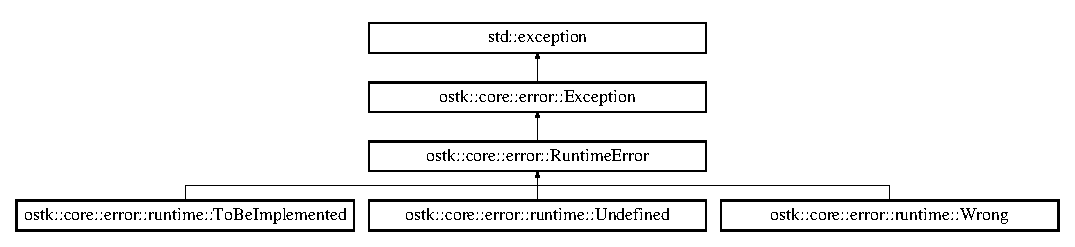
\includegraphics[height=2.871795cm]{classostk_1_1core_1_1error_1_1_exception}
\end{center}
\end{figure}
\subsection*{Public Member Functions}
\begin{DoxyCompactItemize}
\item 
\hyperlink{classostk_1_1core_1_1error_1_1_exception_a27647e55b84a7a32cf8b24e575651d71}{Exception} (const \hyperlink{classostk_1_1core_1_1types_1_1_string}{String} \&a\+Scope)
\item 
\hyperlink{classostk_1_1core_1_1error_1_1_exception_ae44d71ced961433d0b3325ff176e4974}{$\sim$\+Exception} ()
\item 
\hyperlink{classostk_1_1core_1_1types_1_1_string}{String} \hyperlink{classostk_1_1core_1_1error_1_1_exception_a3778009187ea6841eff3bdd45d345144}{get\+Scope} () const
\item 
virtual const char $\ast$ \hyperlink{classostk_1_1core_1_1error_1_1_exception_ae34ebc20a97277da6e2472b6bb8e3812}{what} () const noexcept
\end{DoxyCompactItemize}


\subsection{Detailed Description}
\hyperlink{classostk_1_1core_1_1error_1_1_exception}{Exception} class. 

\subsection{Constructor \& Destructor Documentation}
\mbox{\Hypertarget{classostk_1_1core_1_1error_1_1_exception_a27647e55b84a7a32cf8b24e575651d71}\label{classostk_1_1core_1_1error_1_1_exception_a27647e55b84a7a32cf8b24e575651d71}} 
\index{ostk\+::core\+::error\+::\+Exception@{ostk\+::core\+::error\+::\+Exception}!Exception@{Exception}}
\index{Exception@{Exception}!ostk\+::core\+::error\+::\+Exception@{ostk\+::core\+::error\+::\+Exception}}
\subsubsection{\texorpdfstring{Exception()}{Exception()}}
{\footnotesize\ttfamily ostk\+::core\+::error\+::\+Exception\+::\+Exception (\begin{DoxyParamCaption}\item[{const \hyperlink{classostk_1_1core_1_1types_1_1_string}{String} \&}]{a\+Scope }\end{DoxyParamCaption})}

\mbox{\Hypertarget{classostk_1_1core_1_1error_1_1_exception_ae44d71ced961433d0b3325ff176e4974}\label{classostk_1_1core_1_1error_1_1_exception_ae44d71ced961433d0b3325ff176e4974}} 
\index{ostk\+::core\+::error\+::\+Exception@{ostk\+::core\+::error\+::\+Exception}!````~Exception@{$\sim$\+Exception}}
\index{````~Exception@{$\sim$\+Exception}!ostk\+::core\+::error\+::\+Exception@{ostk\+::core\+::error\+::\+Exception}}
\subsubsection{\texorpdfstring{$\sim$\+Exception()}{~Exception()}}
{\footnotesize\ttfamily ostk\+::core\+::error\+::\+Exception\+::$\sim$\+Exception (\begin{DoxyParamCaption}{ }\end{DoxyParamCaption})}



\subsection{Member Function Documentation}
\mbox{\Hypertarget{classostk_1_1core_1_1error_1_1_exception_a3778009187ea6841eff3bdd45d345144}\label{classostk_1_1core_1_1error_1_1_exception_a3778009187ea6841eff3bdd45d345144}} 
\index{ostk\+::core\+::error\+::\+Exception@{ostk\+::core\+::error\+::\+Exception}!get\+Scope@{get\+Scope}}
\index{get\+Scope@{get\+Scope}!ostk\+::core\+::error\+::\+Exception@{ostk\+::core\+::error\+::\+Exception}}
\subsubsection{\texorpdfstring{get\+Scope()}{getScope()}}
{\footnotesize\ttfamily \hyperlink{classostk_1_1core_1_1types_1_1_string}{String} ostk\+::core\+::error\+::\+Exception\+::get\+Scope (\begin{DoxyParamCaption}{ }\end{DoxyParamCaption}) const}

\mbox{\Hypertarget{classostk_1_1core_1_1error_1_1_exception_ae34ebc20a97277da6e2472b6bb8e3812}\label{classostk_1_1core_1_1error_1_1_exception_ae34ebc20a97277da6e2472b6bb8e3812}} 
\index{ostk\+::core\+::error\+::\+Exception@{ostk\+::core\+::error\+::\+Exception}!what@{what}}
\index{what@{what}!ostk\+::core\+::error\+::\+Exception@{ostk\+::core\+::error\+::\+Exception}}
\subsubsection{\texorpdfstring{what()}{what()}}
{\footnotesize\ttfamily const char $\ast$ ostk\+::core\+::error\+::\+Exception\+::what (\begin{DoxyParamCaption}{ }\end{DoxyParamCaption}) const\hspace{0.3cm}{\ttfamily [virtual]}, {\ttfamily [noexcept]}}



Reimplemented in \hyperlink{classostk_1_1core_1_1error_1_1_runtime_error_a671d71ab5483eaa1ce5cc3400747ded1}{ostk\+::core\+::error\+::\+Runtime\+Error}.



The documentation for this class was generated from the following files\+:\begin{DoxyCompactItemize}
\item 
include/\+Open\+Space\+Toolkit/\+Core/\+Error/\hyperlink{_exception_8hpp}{Exception.\+hpp}\item 
src/\+Open\+Space\+Toolkit/\+Core/\+Error/\hyperlink{_exception_8cpp}{Exception.\+cpp}\end{DoxyCompactItemize}

\hypertarget{classostk_1_1core_1_1fs_1_1_file}{}\section{ostk\+:\+:core\+:\+:fs\+:\+:File Class Reference}
\label{classostk_1_1core_1_1fs_1_1_file}\index{ostk\+::core\+::fs\+::\+File@{ostk\+::core\+::fs\+::\+File}}


Computer resource for recording data discretely in a computer storage device.  




{\ttfamily \#include $<$File.\+hpp$>$}

\subsection*{Public Types}
\begin{DoxyCompactItemize}
\item 
enum \hyperlink{classostk_1_1core_1_1fs_1_1_file_aef3d3e622ef15381a9f48c161e134da5}{Open\+Mode} \{ \newline
\hyperlink{classostk_1_1core_1_1fs_1_1_file_aef3d3e622ef15381a9f48c161e134da5aec0fc0100c4fc1ce4eea230c3dc10360}{Open\+Mode\+::\+Undefined}, 
\hyperlink{classostk_1_1core_1_1fs_1_1_file_aef3d3e622ef15381a9f48c161e134da5a7a1a5f3e79fdc91edf2f5ead9d66abb4}{Open\+Mode\+::\+Read}, 
\hyperlink{classostk_1_1core_1_1fs_1_1_file_aef3d3e622ef15381a9f48c161e134da5a1129c0e4d43f2d121652a7302712cff6}{Open\+Mode\+::\+Write}, 
\hyperlink{classostk_1_1core_1_1fs_1_1_file_aef3d3e622ef15381a9f48c161e134da5a6ce976e8f061b2b5cfe4d0c50c3405dd}{Open\+Mode\+::\+Binary}, 
\newline
\hyperlink{classostk_1_1core_1_1fs_1_1_file_aef3d3e622ef15381a9f48c161e134da5a3ac4692f3935a49a0b243eecf529faa9}{Open\+Mode\+::\+Append}, 
\hyperlink{classostk_1_1core_1_1fs_1_1_file_aef3d3e622ef15381a9f48c161e134da5a8d04b2d09dcc744cf134542097642db5}{Open\+Mode\+::\+At\+End}, 
\hyperlink{classostk_1_1core_1_1fs_1_1_file_aef3d3e622ef15381a9f48c161e134da5aa8156810bfee2bd2b44765b9e91db3bd}{Open\+Mode\+::\+Truncate}
 \}\begin{DoxyCompactList}\small\item\em \hyperlink{classostk_1_1core_1_1fs_1_1_file}{File} open mode. \end{DoxyCompactList}
\end{DoxyCompactItemize}
\subsection*{Public Member Functions}
\begin{DoxyCompactItemize}
\item 
\hyperlink{classostk_1_1core_1_1fs_1_1_file_ad1695224996950be9962b8457da369b3}{File} (const \hyperlink{classostk_1_1core_1_1fs_1_1_file}{File} \&a\+File)
\begin{DoxyCompactList}\small\item\em Copy constructor. \end{DoxyCompactList}\item 
\hyperlink{classostk_1_1core_1_1fs_1_1_file}{File} \& \hyperlink{classostk_1_1core_1_1fs_1_1_file_a497eeaad4b643dc25856e2dcfdda49c4}{operator=} (const \hyperlink{classostk_1_1core_1_1fs_1_1_file}{File} \&a\+File)
\begin{DoxyCompactList}\small\item\em Copy assignment operator. \end{DoxyCompactList}\item 
\hyperlink{classostk_1_1core_1_1fs_1_1_file_afd7c6c0daabedeecc958348d01595b05}{$\sim$\+File} ()
\begin{DoxyCompactList}\small\item\em Destructor. \end{DoxyCompactList}\item 
bool \hyperlink{classostk_1_1core_1_1fs_1_1_file_a293348f9363e8b7544b684ffd12a63f8}{operator==} (const \hyperlink{classostk_1_1core_1_1fs_1_1_file}{File} \&a\+File) const
\begin{DoxyCompactList}\small\item\em Equal to operator. \end{DoxyCompactList}\item 
bool \hyperlink{classostk_1_1core_1_1fs_1_1_file_a96e2f605d1599c6c7368037917ababa9}{operator!=} (const \hyperlink{classostk_1_1core_1_1fs_1_1_file}{File} \&a\+File) const
\begin{DoxyCompactList}\small\item\em Not equal to operator. \end{DoxyCompactList}\item 
{\footnotesize template$<$class T $>$ }\\\hyperlink{classostk_1_1core_1_1fs_1_1_file}{File} \& \hyperlink{classostk_1_1core_1_1fs_1_1_file_a2521124159897934f1a85144511043f7}{operator$<$$<$} (const T \&an\+Object)
\begin{DoxyCompactList}\small\item\em Stream operator. \end{DoxyCompactList}\item 
bool \hyperlink{classostk_1_1core_1_1fs_1_1_file_a35d96a10069d22bc45385fdad04bbe00}{is\+Defined} () const
\begin{DoxyCompactList}\small\item\em Check if file is defined. \end{DoxyCompactList}\item 
bool \hyperlink{classostk_1_1core_1_1fs_1_1_file_afcd8f1b98fbbfe0736f91ddb5e14c4c4}{exists} () const
\begin{DoxyCompactList}\small\item\em Check if file exists. \end{DoxyCompactList}\item 
bool \hyperlink{classostk_1_1core_1_1fs_1_1_file_a6e719c79ddb035206a6b2ce808258f2e}{is\+Open} () const
\begin{DoxyCompactList}\small\item\em Check if file is open. \end{DoxyCompactList}\item 
\hyperlink{classostk_1_1core_1_1types_1_1_string}{String} \hyperlink{classostk_1_1core_1_1fs_1_1_file_ac3120c49b69a93fa364dba012a0d507a}{get\+Name} (const bool with\+Extension=true) const
\begin{DoxyCompactList}\small\item\em Get file name. \end{DoxyCompactList}\item 
\hyperlink{classostk_1_1core_1_1types_1_1_string}{String} \hyperlink{classostk_1_1core_1_1fs_1_1_file_a91123937e378c905d973998e13b61493}{get\+Extension} () const
\begin{DoxyCompactList}\small\item\em Get file extension. \end{DoxyCompactList}\item 
\hyperlink{classostk_1_1core_1_1fs_1_1_path}{fs\+::\+Path} \hyperlink{classostk_1_1core_1_1fs_1_1_file_a4bdf46eada08ce70e2a408606aab94e4}{get\+Path} () const
\begin{DoxyCompactList}\small\item\em Get file path. \end{DoxyCompactList}\item 
\hyperlink{classostk_1_1core_1_1fs_1_1_permission_set}{fs\+::\+Permission\+Set} \hyperlink{classostk_1_1core_1_1fs_1_1_file_aded4a0f23b9c81f12e2ce3f4e95f3bd0}{get\+Permissions} () const
\begin{DoxyCompactList}\small\item\em Get file permissions. \end{DoxyCompactList}\item 
\hyperlink{classostk_1_1core_1_1fs_1_1_directory}{fs\+::\+Directory} \hyperlink{classostk_1_1core_1_1fs_1_1_file_a90626395dbeab369d76255556600c7cc}{get\+Parent\+Directory} () const
\begin{DoxyCompactList}\small\item\em Get file\textquotesingle{}s parent directory. \end{DoxyCompactList}\item 
\hyperlink{classostk_1_1core_1_1types_1_1_string}{String} \hyperlink{classostk_1_1core_1_1fs_1_1_file_a4ce7db90e409818e3c4d2b27884260cf}{get\+Contents} () const
\begin{DoxyCompactList}\small\item\em Get file contents. \end{DoxyCompactList}\item 
\hyperlink{classostk_1_1core_1_1types_1_1_string}{String} \hyperlink{classostk_1_1core_1_1fs_1_1_file_af3fc4659467e9eba1a7faff578abdbab}{to\+String} () const
\begin{DoxyCompactList}\small\item\em Get serialized file. \end{DoxyCompactList}\item 
void \hyperlink{classostk_1_1core_1_1fs_1_1_file_a3d5b7ddfa15dde13573f904900cd84e6}{open} (const \hyperlink{classostk_1_1core_1_1fs_1_1_file_aef3d3e622ef15381a9f48c161e134da5}{File\+::\+Open\+Mode} \&an\+Open\+Mode)
\begin{DoxyCompactList}\small\item\em Open file. \end{DoxyCompactList}\item 
void \hyperlink{classostk_1_1core_1_1fs_1_1_file_a1673393d876005d7eae90e435584ea38}{close} ()
\begin{DoxyCompactList}\small\item\em Close file. \end{DoxyCompactList}\item 
std\+::fstream \& \hyperlink{classostk_1_1core_1_1fs_1_1_file_a0a6494f47ca7384d29f6b318d0380dfc}{access\+Stream} ()
\begin{DoxyCompactList}\small\item\em Access file stream. \end{DoxyCompactList}\item 
void \hyperlink{classostk_1_1core_1_1fs_1_1_file_ab1afed5cc78b78359201b587a4b63307}{rename\+To} (const \hyperlink{classostk_1_1core_1_1types_1_1_string}{String} \&a\+Name)
\begin{DoxyCompactList}\small\item\em Rename file. \end{DoxyCompactList}\item 
\hyperlink{classostk_1_1core_1_1fs_1_1_file}{File} \hyperlink{classostk_1_1core_1_1fs_1_1_file_aab6e069ef912f0ffe6203a9eb32a16d7}{copy\+To\+Directory} (const \hyperlink{classostk_1_1core_1_1fs_1_1_directory}{fs\+::\+Directory} \&a\+Destination, const \hyperlink{classostk_1_1core_1_1types_1_1_string}{String} \&a\+New\+File\+Name=\char`\"{}\char`\"{}) const
\begin{DoxyCompactList}\small\item\em Copy file to directory. \end{DoxyCompactList}\item 
void \hyperlink{classostk_1_1core_1_1fs_1_1_file_a30689af3e982cf9ae611312695b812ab}{move\+To\+Directory} (const \hyperlink{classostk_1_1core_1_1fs_1_1_directory}{fs\+::\+Directory} \&a\+Destination)
\begin{DoxyCompactList}\small\item\em Move file to directory. \end{DoxyCompactList}\item 
void \hyperlink{classostk_1_1core_1_1fs_1_1_file_ad02a3565af878feb290667b071497749}{create} (const \hyperlink{classostk_1_1core_1_1fs_1_1_permission_set}{fs\+::\+Permission\+Set} \&an\+Owner\+Permission\+Set=\hyperlink{classostk_1_1core_1_1fs_1_1_permission_set_ad58bc0911ca89d3c03c089f1647d0315}{fs\+::\+Permission\+Set\+::\+RW}(), const \hyperlink{classostk_1_1core_1_1fs_1_1_permission_set}{fs\+::\+Permission\+Set} \&a\+Group\+Permission\+Set=\hyperlink{classostk_1_1core_1_1fs_1_1_permission_set_a400f8be607966c0a42597f5cef062210}{fs\+::\+Permission\+Set\+::R}(), const \hyperlink{classostk_1_1core_1_1fs_1_1_permission_set}{fs\+::\+Permission\+Set} \&an\+Other\+Permission\+Set=\hyperlink{classostk_1_1core_1_1fs_1_1_permission_set_a400f8be607966c0a42597f5cef062210}{fs\+::\+Permission\+Set\+::R}())
\begin{DoxyCompactList}\small\item\em Create empty file. \end{DoxyCompactList}\item 
void \hyperlink{classostk_1_1core_1_1fs_1_1_file_a10f822f5146c5ee5fe43e35bfd39f88e}{clear} ()
\begin{DoxyCompactList}\small\item\em Clear file contents. \end{DoxyCompactList}\item 
void \hyperlink{classostk_1_1core_1_1fs_1_1_file_a08ab15296e2baa61e7a023514cb46f31}{remove} ()
\begin{DoxyCompactList}\small\item\em Delete file. \end{DoxyCompactList}\end{DoxyCompactItemize}
\subsection*{Static Public Member Functions}
\begin{DoxyCompactItemize}
\item 
static \hyperlink{classostk_1_1core_1_1fs_1_1_file}{File} \hyperlink{classostk_1_1core_1_1fs_1_1_file_a0df3ba12f33cbbd8f24b9d35cd4afaee}{Undefined} ()
\begin{DoxyCompactList}\small\item\em Constructs an undefined file. \end{DoxyCompactList}\item 
static \hyperlink{classostk_1_1core_1_1fs_1_1_file}{File} \hyperlink{classostk_1_1core_1_1fs_1_1_file_ad677c6a3edc1e88c18226edebff1da03}{Path} (const \hyperlink{classostk_1_1core_1_1fs_1_1_path}{fs\+::\+Path} \&a\+Path)
\begin{DoxyCompactList}\small\item\em Constructs a file from a given path. \end{DoxyCompactList}\end{DoxyCompactItemize}
\subsection*{Friends}
\begin{DoxyCompactItemize}
\item 
std\+::ostream \& \hyperlink{classostk_1_1core_1_1fs_1_1_file_a82ce9f27653427d53ecb90de978f4f68}{operator$<$$<$} (std\+::ostream \&an\+Output\+Stream, const \hyperlink{classostk_1_1core_1_1fs_1_1_file}{File} \&a\+File)
\begin{DoxyCompactList}\small\item\em Output stream operator. \end{DoxyCompactList}\end{DoxyCompactItemize}


\subsection{Detailed Description}
Computer resource for recording data discretely in a computer storage device. 

https\+://en.wikipedia.\+org/wiki/\+Computer\+\_\+file 

\subsection{Member Enumeration Documentation}
\mbox{\Hypertarget{classostk_1_1core_1_1fs_1_1_file_aef3d3e622ef15381a9f48c161e134da5}\label{classostk_1_1core_1_1fs_1_1_file_aef3d3e622ef15381a9f48c161e134da5}} 
\index{ostk\+::core\+::fs\+::\+File@{ostk\+::core\+::fs\+::\+File}!Open\+Mode@{Open\+Mode}}
\index{Open\+Mode@{Open\+Mode}!ostk\+::core\+::fs\+::\+File@{ostk\+::core\+::fs\+::\+File}}
\subsubsection{\texorpdfstring{Open\+Mode}{OpenMode}}
{\footnotesize\ttfamily enum \hyperlink{classostk_1_1core_1_1fs_1_1_file_aef3d3e622ef15381a9f48c161e134da5}{ostk\+::core\+::fs\+::\+File\+::\+Open\+Mode}\hspace{0.3cm}{\ttfamily [strong]}}



\hyperlink{classostk_1_1core_1_1fs_1_1_file}{File} open mode. 

\begin{DoxyEnumFields}{Enumerator}
\raisebox{\heightof{T}}[0pt][0pt]{\index{Undefined@{Undefined}!ostk\+::core\+::fs\+::\+File@{ostk\+::core\+::fs\+::\+File}}\index{ostk\+::core\+::fs\+::\+File@{ostk\+::core\+::fs\+::\+File}!Undefined@{Undefined}}}\mbox{\Hypertarget{classostk_1_1core_1_1fs_1_1_file_aef3d3e622ef15381a9f48c161e134da5aec0fc0100c4fc1ce4eea230c3dc10360}\label{classostk_1_1core_1_1fs_1_1_file_aef3d3e622ef15381a9f48c161e134da5aec0fc0100c4fc1ce4eea230c3dc10360}} 
Undefined&Undefined mode. \\
\hline

\raisebox{\heightof{T}}[0pt][0pt]{\index{Read@{Read}!ostk\+::core\+::fs\+::\+File@{ostk\+::core\+::fs\+::\+File}}\index{ostk\+::core\+::fs\+::\+File@{ostk\+::core\+::fs\+::\+File}!Read@{Read}}}\mbox{\Hypertarget{classostk_1_1core_1_1fs_1_1_file_aef3d3e622ef15381a9f48c161e134da5a7a1a5f3e79fdc91edf2f5ead9d66abb4}\label{classostk_1_1core_1_1fs_1_1_file_aef3d3e622ef15381a9f48c161e134da5a7a1a5f3e79fdc91edf2f5ead9d66abb4}} 
Read&Open for reading. \\
\hline

\raisebox{\heightof{T}}[0pt][0pt]{\index{Write@{Write}!ostk\+::core\+::fs\+::\+File@{ostk\+::core\+::fs\+::\+File}}\index{ostk\+::core\+::fs\+::\+File@{ostk\+::core\+::fs\+::\+File}!Write@{Write}}}\mbox{\Hypertarget{classostk_1_1core_1_1fs_1_1_file_aef3d3e622ef15381a9f48c161e134da5a1129c0e4d43f2d121652a7302712cff6}\label{classostk_1_1core_1_1fs_1_1_file_aef3d3e622ef15381a9f48c161e134da5a1129c0e4d43f2d121652a7302712cff6}} 
Write&Open for writing. \\
\hline

\raisebox{\heightof{T}}[0pt][0pt]{\index{Binary@{Binary}!ostk\+::core\+::fs\+::\+File@{ostk\+::core\+::fs\+::\+File}}\index{ostk\+::core\+::fs\+::\+File@{ostk\+::core\+::fs\+::\+File}!Binary@{Binary}}}\mbox{\Hypertarget{classostk_1_1core_1_1fs_1_1_file_aef3d3e622ef15381a9f48c161e134da5a6ce976e8f061b2b5cfe4d0c50c3405dd}\label{classostk_1_1core_1_1fs_1_1_file_aef3d3e622ef15381a9f48c161e134da5a6ce976e8f061b2b5cfe4d0c50c3405dd}} 
Binary&Open in binary mode. \\
\hline

\raisebox{\heightof{T}}[0pt][0pt]{\index{Append@{Append}!ostk\+::core\+::fs\+::\+File@{ostk\+::core\+::fs\+::\+File}}\index{ostk\+::core\+::fs\+::\+File@{ostk\+::core\+::fs\+::\+File}!Append@{Append}}}\mbox{\Hypertarget{classostk_1_1core_1_1fs_1_1_file_aef3d3e622ef15381a9f48c161e134da5a3ac4692f3935a49a0b243eecf529faa9}\label{classostk_1_1core_1_1fs_1_1_file_aef3d3e622ef15381a9f48c161e134da5a3ac4692f3935a49a0b243eecf529faa9}} 
Append&Seek to the end of stream before each write. \\
\hline

\raisebox{\heightof{T}}[0pt][0pt]{\index{At\+End@{At\+End}!ostk\+::core\+::fs\+::\+File@{ostk\+::core\+::fs\+::\+File}}\index{ostk\+::core\+::fs\+::\+File@{ostk\+::core\+::fs\+::\+File}!At\+End@{At\+End}}}\mbox{\Hypertarget{classostk_1_1core_1_1fs_1_1_file_aef3d3e622ef15381a9f48c161e134da5a8d04b2d09dcc744cf134542097642db5}\label{classostk_1_1core_1_1fs_1_1_file_aef3d3e622ef15381a9f48c161e134da5a8d04b2d09dcc744cf134542097642db5}} 
At\+End&Seek to the end of stream immediately after open. \\
\hline

\raisebox{\heightof{T}}[0pt][0pt]{\index{Truncate@{Truncate}!ostk\+::core\+::fs\+::\+File@{ostk\+::core\+::fs\+::\+File}}\index{ostk\+::core\+::fs\+::\+File@{ostk\+::core\+::fs\+::\+File}!Truncate@{Truncate}}}\mbox{\Hypertarget{classostk_1_1core_1_1fs_1_1_file_aef3d3e622ef15381a9f48c161e134da5aa8156810bfee2bd2b44765b9e91db3bd}\label{classostk_1_1core_1_1fs_1_1_file_aef3d3e622ef15381a9f48c161e134da5aa8156810bfee2bd2b44765b9e91db3bd}} 
Truncate&Discard the contents of the stream when opening. \\
\hline

\end{DoxyEnumFields}


\subsection{Constructor \& Destructor Documentation}
\mbox{\Hypertarget{classostk_1_1core_1_1fs_1_1_file_ad1695224996950be9962b8457da369b3}\label{classostk_1_1core_1_1fs_1_1_file_ad1695224996950be9962b8457da369b3}} 
\index{ostk\+::core\+::fs\+::\+File@{ostk\+::core\+::fs\+::\+File}!File@{File}}
\index{File@{File}!ostk\+::core\+::fs\+::\+File@{ostk\+::core\+::fs\+::\+File}}
\subsubsection{\texorpdfstring{File()}{File()}}
{\footnotesize\ttfamily ostk\+::core\+::fs\+::\+File\+::\+File (\begin{DoxyParamCaption}\item[{const \hyperlink{classostk_1_1core_1_1fs_1_1_file}{File} \&}]{a\+File }\end{DoxyParamCaption})}



Copy constructor. 


\begin{DoxyParams}[1]{Parameters}
\mbox{\tt in}  & {\em a\+File} & A file \\
\hline
\end{DoxyParams}
\mbox{\Hypertarget{classostk_1_1core_1_1fs_1_1_file_afd7c6c0daabedeecc958348d01595b05}\label{classostk_1_1core_1_1fs_1_1_file_afd7c6c0daabedeecc958348d01595b05}} 
\index{ostk\+::core\+::fs\+::\+File@{ostk\+::core\+::fs\+::\+File}!````~File@{$\sim$\+File}}
\index{````~File@{$\sim$\+File}!ostk\+::core\+::fs\+::\+File@{ostk\+::core\+::fs\+::\+File}}
\subsubsection{\texorpdfstring{$\sim$\+File()}{~File()}}
{\footnotesize\ttfamily ostk\+::core\+::fs\+::\+File\+::$\sim$\+File (\begin{DoxyParamCaption}{ }\end{DoxyParamCaption})}



Destructor. 



\subsection{Member Function Documentation}
\mbox{\Hypertarget{classostk_1_1core_1_1fs_1_1_file_a0a6494f47ca7384d29f6b318d0380dfc}\label{classostk_1_1core_1_1fs_1_1_file_a0a6494f47ca7384d29f6b318d0380dfc}} 
\index{ostk\+::core\+::fs\+::\+File@{ostk\+::core\+::fs\+::\+File}!access\+Stream@{access\+Stream}}
\index{access\+Stream@{access\+Stream}!ostk\+::core\+::fs\+::\+File@{ostk\+::core\+::fs\+::\+File}}
\subsubsection{\texorpdfstring{access\+Stream()}{accessStream()}}
{\footnotesize\ttfamily std\+::fstream \& ostk\+::core\+::fs\+::\+File\+::access\+Stream (\begin{DoxyParamCaption}{ }\end{DoxyParamCaption})}



Access file stream. 

\begin{DoxyReturn}{Returns}
Reference to file stream 
\end{DoxyReturn}
\mbox{\Hypertarget{classostk_1_1core_1_1fs_1_1_file_a10f822f5146c5ee5fe43e35bfd39f88e}\label{classostk_1_1core_1_1fs_1_1_file_a10f822f5146c5ee5fe43e35bfd39f88e}} 
\index{ostk\+::core\+::fs\+::\+File@{ostk\+::core\+::fs\+::\+File}!clear@{clear}}
\index{clear@{clear}!ostk\+::core\+::fs\+::\+File@{ostk\+::core\+::fs\+::\+File}}
\subsubsection{\texorpdfstring{clear()}{clear()}}
{\footnotesize\ttfamily void ostk\+::core\+::fs\+::\+File\+::clear (\begin{DoxyParamCaption}{ }\end{DoxyParamCaption})}



Clear file contents. 


\begin{DoxyCode}
\hyperlink{classostk_1_1core_1_1fs_1_1_file_ad1695224996950be9962b8457da369b3}{File} file = \hyperlink{classostk_1_1core_1_1fs_1_1_file_ad677c6a3edc1e88c18226edebff1da03}{File::Path}(\hyperlink{classostk_1_1core_1_1fs_1_1_path_ad08539ba654f5df11c4bcb07276345ad}{Path::Parse}(\textcolor{stringliteral}{"/path/to/file.txt"})) ;
file.exists() ; \textcolor{comment}{// True}
file.clear() ;
file.exists() ; \textcolor{comment}{// True}
\end{DoxyCode}
 \mbox{\Hypertarget{classostk_1_1core_1_1fs_1_1_file_a1673393d876005d7eae90e435584ea38}\label{classostk_1_1core_1_1fs_1_1_file_a1673393d876005d7eae90e435584ea38}} 
\index{ostk\+::core\+::fs\+::\+File@{ostk\+::core\+::fs\+::\+File}!close@{close}}
\index{close@{close}!ostk\+::core\+::fs\+::\+File@{ostk\+::core\+::fs\+::\+File}}
\subsubsection{\texorpdfstring{close()}{close()}}
{\footnotesize\ttfamily void ostk\+::core\+::fs\+::\+File\+::close (\begin{DoxyParamCaption}{ }\end{DoxyParamCaption})}



Close file. 

\mbox{\Hypertarget{classostk_1_1core_1_1fs_1_1_file_aab6e069ef912f0ffe6203a9eb32a16d7}\label{classostk_1_1core_1_1fs_1_1_file_aab6e069ef912f0ffe6203a9eb32a16d7}} 
\index{ostk\+::core\+::fs\+::\+File@{ostk\+::core\+::fs\+::\+File}!copy\+To\+Directory@{copy\+To\+Directory}}
\index{copy\+To\+Directory@{copy\+To\+Directory}!ostk\+::core\+::fs\+::\+File@{ostk\+::core\+::fs\+::\+File}}
\subsubsection{\texorpdfstring{copy\+To\+Directory()}{copyToDirectory()}}
{\footnotesize\ttfamily \hyperlink{classostk_1_1core_1_1fs_1_1_file}{File} ostk\+::core\+::fs\+::\+File\+::copy\+To\+Directory (\begin{DoxyParamCaption}\item[{const \hyperlink{classostk_1_1core_1_1fs_1_1_directory}{fs\+::\+Directory} \&}]{a\+Destination,  }\item[{const \hyperlink{classostk_1_1core_1_1types_1_1_string}{String} \&}]{a\+New\+File\+Name = {\ttfamily \char`\"{}\char`\"{}} }\end{DoxyParamCaption}) const}



Copy file to directory. 


\begin{DoxyCode}
\hyperlink{classostk_1_1core_1_1fs_1_1_file_ad1695224996950be9962b8457da369b3}{File} original = \hyperlink{classostk_1_1core_1_1fs_1_1_file_ad677c6a3edc1e88c18226edebff1da03}{File::Path}(\hyperlink{classostk_1_1core_1_1fs_1_1_path_ad08539ba654f5df11c4bcb07276345ad}{Path::Parse}(\textcolor{stringliteral}{"/path/to/file.txt"})) ;
Directory destination = \hyperlink{classostk_1_1core_1_1fs_1_1_directory_a0151dba2940d5f426b52209dc7dab2e5}{Directory::Path}(\hyperlink{classostk_1_1core_1_1fs_1_1_path_ad08539ba654f5df11c4bcb07276345ad}{Path::Parse}(\textcolor{stringliteral}{"/new/path/to"})) ;
\hyperlink{classostk_1_1core_1_1fs_1_1_file_ad1695224996950be9962b8457da369b3}{File} copy = original.copyToDirectory(destination) ; \textcolor{comment}{// /new/path/to/file.txt}
\end{DoxyCode}



\begin{DoxyParams}[1]{Parameters}
\mbox{\tt in}  & {\em a\+Destination} & A destination directory \\
\hline
\mbox{\tt in}  & {\em (optional)} & a\+New\+File\+Name A copied file name \\
\hline
\end{DoxyParams}
\begin{DoxyReturn}{Returns}
Copied file 
\end{DoxyReturn}
\mbox{\Hypertarget{classostk_1_1core_1_1fs_1_1_file_ad02a3565af878feb290667b071497749}\label{classostk_1_1core_1_1fs_1_1_file_ad02a3565af878feb290667b071497749}} 
\index{ostk\+::core\+::fs\+::\+File@{ostk\+::core\+::fs\+::\+File}!create@{create}}
\index{create@{create}!ostk\+::core\+::fs\+::\+File@{ostk\+::core\+::fs\+::\+File}}
\subsubsection{\texorpdfstring{create()}{create()}}
{\footnotesize\ttfamily void ostk\+::core\+::fs\+::\+File\+::create (\begin{DoxyParamCaption}\item[{const \hyperlink{classostk_1_1core_1_1fs_1_1_permission_set}{fs\+::\+Permission\+Set} \&}]{an\+Owner\+Permission\+Set = {\ttfamily \hyperlink{classostk_1_1core_1_1fs_1_1_permission_set_ad58bc0911ca89d3c03c089f1647d0315}{fs\+::\+Permission\+Set\+::\+RW}()},  }\item[{const \hyperlink{classostk_1_1core_1_1fs_1_1_permission_set}{fs\+::\+Permission\+Set} \&}]{a\+Group\+Permission\+Set = {\ttfamily \hyperlink{classostk_1_1core_1_1fs_1_1_permission_set_a400f8be607966c0a42597f5cef062210}{fs\+::\+Permission\+Set\+::R}()},  }\item[{const \hyperlink{classostk_1_1core_1_1fs_1_1_permission_set}{fs\+::\+Permission\+Set} \&}]{an\+Other\+Permission\+Set = {\ttfamily \hyperlink{classostk_1_1core_1_1fs_1_1_permission_set_a400f8be607966c0a42597f5cef062210}{fs\+::\+Permission\+Set\+::R}()} }\end{DoxyParamCaption})}



Create empty file. 


\begin{DoxyCode}
\hyperlink{classostk_1_1core_1_1fs_1_1_file_ad1695224996950be9962b8457da369b3}{File} file = \hyperlink{classostk_1_1core_1_1fs_1_1_file_ad677c6a3edc1e88c18226edebff1da03}{File::Path}(\hyperlink{classostk_1_1core_1_1fs_1_1_path_ad08539ba654f5df11c4bcb07276345ad}{Path::Parse}(\textcolor{stringliteral}{"/path/to/file.txt"})) ;
file.exists() ; \textcolor{comment}{// False}
file.create() ;
file.exists() ; \textcolor{comment}{// True}
\end{DoxyCode}



\begin{DoxyParams}[1]{Parameters}
\mbox{\tt in}  & {\em (optional)} & an\+Owner\+Permission\+Set An owner permission set \\
\hline
\mbox{\tt in}  & {\em (optional)} & a\+Group\+Permission\+Set A group permission set \\
\hline
\mbox{\tt in}  & {\em (optional)} & an\+Other\+Permission\+Set An other permission set \\
\hline
\end{DoxyParams}
\mbox{\Hypertarget{classostk_1_1core_1_1fs_1_1_file_afcd8f1b98fbbfe0736f91ddb5e14c4c4}\label{classostk_1_1core_1_1fs_1_1_file_afcd8f1b98fbbfe0736f91ddb5e14c4c4}} 
\index{ostk\+::core\+::fs\+::\+File@{ostk\+::core\+::fs\+::\+File}!exists@{exists}}
\index{exists@{exists}!ostk\+::core\+::fs\+::\+File@{ostk\+::core\+::fs\+::\+File}}
\subsubsection{\texorpdfstring{exists()}{exists()}}
{\footnotesize\ttfamily bool ostk\+::core\+::fs\+::\+File\+::exists (\begin{DoxyParamCaption}{ }\end{DoxyParamCaption}) const}



Check if file exists. 


\begin{DoxyCode}
\hyperlink{classostk_1_1core_1_1fs_1_1_file_ad1695224996950be9962b8457da369b3}{File} file = \hyperlink{classostk_1_1core_1_1fs_1_1_file_ad677c6a3edc1e88c18226edebff1da03}{File::Path}(\hyperlink{classostk_1_1core_1_1fs_1_1_path_ad08539ba654f5df11c4bcb07276345ad}{Path::Parse}(\textcolor{stringliteral}{"/path/to/nonexistent/file"})) ;
file.exists() ; \textcolor{comment}{// False}
\end{DoxyCode}


\begin{DoxyReturn}{Returns}
True if file exists 
\end{DoxyReturn}
\mbox{\Hypertarget{classostk_1_1core_1_1fs_1_1_file_a4ce7db90e409818e3c4d2b27884260cf}\label{classostk_1_1core_1_1fs_1_1_file_a4ce7db90e409818e3c4d2b27884260cf}} 
\index{ostk\+::core\+::fs\+::\+File@{ostk\+::core\+::fs\+::\+File}!get\+Contents@{get\+Contents}}
\index{get\+Contents@{get\+Contents}!ostk\+::core\+::fs\+::\+File@{ostk\+::core\+::fs\+::\+File}}
\subsubsection{\texorpdfstring{get\+Contents()}{getContents()}}
{\footnotesize\ttfamily \hyperlink{classostk_1_1core_1_1types_1_1_string}{String} ostk\+::core\+::fs\+::\+File\+::get\+Contents (\begin{DoxyParamCaption}{ }\end{DoxyParamCaption}) const}



Get file contents. 

\begin{DoxyReturn}{Returns}
\hyperlink{classostk_1_1core_1_1fs_1_1_file}{File} contents 
\end{DoxyReturn}
\mbox{\Hypertarget{classostk_1_1core_1_1fs_1_1_file_a91123937e378c905d973998e13b61493}\label{classostk_1_1core_1_1fs_1_1_file_a91123937e378c905d973998e13b61493}} 
\index{ostk\+::core\+::fs\+::\+File@{ostk\+::core\+::fs\+::\+File}!get\+Extension@{get\+Extension}}
\index{get\+Extension@{get\+Extension}!ostk\+::core\+::fs\+::\+File@{ostk\+::core\+::fs\+::\+File}}
\subsubsection{\texorpdfstring{get\+Extension()}{getExtension()}}
{\footnotesize\ttfamily \hyperlink{classostk_1_1core_1_1types_1_1_string}{String} ostk\+::core\+::fs\+::\+File\+::get\+Extension (\begin{DoxyParamCaption}{ }\end{DoxyParamCaption}) const}



Get file extension. 


\begin{DoxyCode}
\hyperlink{classostk_1_1core_1_1fs_1_1_file_ad1695224996950be9962b8457da369b3}{File} file = \hyperlink{classostk_1_1core_1_1fs_1_1_file_ad677c6a3edc1e88c18226edebff1da03}{File::Path}(\hyperlink{classostk_1_1core_1_1fs_1_1_path_ad08539ba654f5df11c4bcb07276345ad}{Path::Parse}(\textcolor{stringliteral}{"/path/to/file.txt"})) ;
file.getExtension() ; \textcolor{comment}{// txt}
\end{DoxyCode}


\begin{DoxyReturn}{Returns}
\hyperlink{classostk_1_1core_1_1fs_1_1_file}{File} extension 
\end{DoxyReturn}
\mbox{\Hypertarget{classostk_1_1core_1_1fs_1_1_file_ac3120c49b69a93fa364dba012a0d507a}\label{classostk_1_1core_1_1fs_1_1_file_ac3120c49b69a93fa364dba012a0d507a}} 
\index{ostk\+::core\+::fs\+::\+File@{ostk\+::core\+::fs\+::\+File}!get\+Name@{get\+Name}}
\index{get\+Name@{get\+Name}!ostk\+::core\+::fs\+::\+File@{ostk\+::core\+::fs\+::\+File}}
\subsubsection{\texorpdfstring{get\+Name()}{getName()}}
{\footnotesize\ttfamily \hyperlink{classostk_1_1core_1_1types_1_1_string}{String} ostk\+::core\+::fs\+::\+File\+::get\+Name (\begin{DoxyParamCaption}\item[{const bool}]{with\+Extension = {\ttfamily true} }\end{DoxyParamCaption}) const}



Get file name. 


\begin{DoxyCode}
\hyperlink{classostk_1_1core_1_1fs_1_1_file_ad1695224996950be9962b8457da369b3}{File} file = \hyperlink{classostk_1_1core_1_1fs_1_1_file_ad677c6a3edc1e88c18226edebff1da03}{File::Path}(\hyperlink{classostk_1_1core_1_1fs_1_1_path_ad08539ba654f5df11c4bcb07276345ad}{Path::Parse}(\textcolor{stringliteral}{"/path/to/file.txt"})) ;
file.getName() ; \textcolor{comment}{// file.txt}
file.getName(\textcolor{keyword}{false}) ; \textcolor{comment}{// file}
\end{DoxyCode}



\begin{DoxyParams}[1]{Parameters}
\mbox{\tt in}  & {\em (optional)} & with\+Extension If true, add extension to filename \\
\hline
\end{DoxyParams}
\begin{DoxyReturn}{Returns}
\hyperlink{classostk_1_1core_1_1fs_1_1_file}{File} name 
\end{DoxyReturn}
\mbox{\Hypertarget{classostk_1_1core_1_1fs_1_1_file_a90626395dbeab369d76255556600c7cc}\label{classostk_1_1core_1_1fs_1_1_file_a90626395dbeab369d76255556600c7cc}} 
\index{ostk\+::core\+::fs\+::\+File@{ostk\+::core\+::fs\+::\+File}!get\+Parent\+Directory@{get\+Parent\+Directory}}
\index{get\+Parent\+Directory@{get\+Parent\+Directory}!ostk\+::core\+::fs\+::\+File@{ostk\+::core\+::fs\+::\+File}}
\subsubsection{\texorpdfstring{get\+Parent\+Directory()}{getParentDirectory()}}
{\footnotesize\ttfamily \hyperlink{classostk_1_1core_1_1fs_1_1_directory}{fs\+::\+Directory} ostk\+::core\+::fs\+::\+File\+::get\+Parent\+Directory (\begin{DoxyParamCaption}{ }\end{DoxyParamCaption}) const}



Get file\textquotesingle{}s parent directory. 


\begin{DoxyCode}
\hyperlink{classostk_1_1core_1_1fs_1_1_file_ad1695224996950be9962b8457da369b3}{File} file = \hyperlink{classostk_1_1core_1_1fs_1_1_file_ad677c6a3edc1e88c18226edebff1da03}{File::Path}(\hyperlink{classostk_1_1core_1_1fs_1_1_path_ad08539ba654f5df11c4bcb07276345ad}{Path::Parse}(\textcolor{stringliteral}{"/path/to/file.txt"})) ;
Directory directory = file.getParentDirectory() ; \textcolor{comment}{// /path/to}
\end{DoxyCode}


\begin{DoxyReturn}{Returns}
\hyperlink{classostk_1_1core_1_1fs_1_1_file}{File}\textquotesingle{}s parent directory 
\end{DoxyReturn}
\mbox{\Hypertarget{classostk_1_1core_1_1fs_1_1_file_a4bdf46eada08ce70e2a408606aab94e4}\label{classostk_1_1core_1_1fs_1_1_file_a4bdf46eada08ce70e2a408606aab94e4}} 
\index{ostk\+::core\+::fs\+::\+File@{ostk\+::core\+::fs\+::\+File}!get\+Path@{get\+Path}}
\index{get\+Path@{get\+Path}!ostk\+::core\+::fs\+::\+File@{ostk\+::core\+::fs\+::\+File}}
\subsubsection{\texorpdfstring{get\+Path()}{getPath()}}
{\footnotesize\ttfamily \hyperlink{classostk_1_1core_1_1fs_1_1_path}{fs\+::\+Path} ostk\+::core\+::fs\+::\+File\+::get\+Path (\begin{DoxyParamCaption}{ }\end{DoxyParamCaption}) const}



Get file path. 


\begin{DoxyCode}
\hyperlink{classostk_1_1core_1_1fs_1_1_file_ad1695224996950be9962b8457da369b3}{File} file = \hyperlink{classostk_1_1core_1_1fs_1_1_file_ad677c6a3edc1e88c18226edebff1da03}{File::Path}(\hyperlink{classostk_1_1core_1_1fs_1_1_path_ad08539ba654f5df11c4bcb07276345ad}{Path::Parse}(\textcolor{stringliteral}{"/path/to/file.txt"})) ;
\hyperlink{classostk_1_1core_1_1fs_1_1_file_ad677c6a3edc1e88c18226edebff1da03}{Path} path = file.\hyperlink{classostk_1_1core_1_1fs_1_1_file_a4bdf46eada08ce70e2a408606aab94e4}{getPath}() ; \textcolor{comment}{// /path/to/file.txt}
\end{DoxyCode}


\begin{DoxyReturn}{Returns}
\hyperlink{classostk_1_1core_1_1fs_1_1_file}{File} path 
\end{DoxyReturn}
\mbox{\Hypertarget{classostk_1_1core_1_1fs_1_1_file_aded4a0f23b9c81f12e2ce3f4e95f3bd0}\label{classostk_1_1core_1_1fs_1_1_file_aded4a0f23b9c81f12e2ce3f4e95f3bd0}} 
\index{ostk\+::core\+::fs\+::\+File@{ostk\+::core\+::fs\+::\+File}!get\+Permissions@{get\+Permissions}}
\index{get\+Permissions@{get\+Permissions}!ostk\+::core\+::fs\+::\+File@{ostk\+::core\+::fs\+::\+File}}
\subsubsection{\texorpdfstring{get\+Permissions()}{getPermissions()}}
{\footnotesize\ttfamily \hyperlink{classostk_1_1core_1_1fs_1_1_permission_set}{fs\+::\+Permission\+Set} ostk\+::core\+::fs\+::\+File\+::get\+Permissions (\begin{DoxyParamCaption}{ }\end{DoxyParamCaption}) const}



Get file permissions. 


\begin{DoxyCode}
\hyperlink{classostk_1_1core_1_1fs_1_1_file_ad1695224996950be9962b8457da369b3}{File} file = \hyperlink{classostk_1_1core_1_1fs_1_1_file_ad677c6a3edc1e88c18226edebff1da03}{File::Path}(\hyperlink{classostk_1_1core_1_1fs_1_1_path_ad08539ba654f5df11c4bcb07276345ad}{Path::Parse}(\textcolor{stringliteral}{"/path/to/file.txt"})) ;
Permissions permissions = file.getPermissions() ; \textcolor{comment}{// rw-}
\end{DoxyCode}


\begin{DoxyReturn}{Returns}
\hyperlink{classostk_1_1core_1_1fs_1_1_file}{File} permissions 
\end{DoxyReturn}
\mbox{\Hypertarget{classostk_1_1core_1_1fs_1_1_file_a35d96a10069d22bc45385fdad04bbe00}\label{classostk_1_1core_1_1fs_1_1_file_a35d96a10069d22bc45385fdad04bbe00}} 
\index{ostk\+::core\+::fs\+::\+File@{ostk\+::core\+::fs\+::\+File}!is\+Defined@{is\+Defined}}
\index{is\+Defined@{is\+Defined}!ostk\+::core\+::fs\+::\+File@{ostk\+::core\+::fs\+::\+File}}
\subsubsection{\texorpdfstring{is\+Defined()}{isDefined()}}
{\footnotesize\ttfamily bool ostk\+::core\+::fs\+::\+File\+::is\+Defined (\begin{DoxyParamCaption}{ }\end{DoxyParamCaption}) const}



Check if file is defined. 


\begin{DoxyCode}
\hyperlink{classostk_1_1core_1_1fs_1_1_file_ad1695224996950be9962b8457da369b3}{File} file = \hyperlink{classostk_1_1core_1_1fs_1_1_file_a0df3ba12f33cbbd8f24b9d35cd4afaee}{File::Undefined}() ;
file.isDefined() ; \textcolor{comment}{// False}
\end{DoxyCode}


\begin{DoxyReturn}{Returns}
True if file is defined 
\end{DoxyReturn}
\mbox{\Hypertarget{classostk_1_1core_1_1fs_1_1_file_a6e719c79ddb035206a6b2ce808258f2e}\label{classostk_1_1core_1_1fs_1_1_file_a6e719c79ddb035206a6b2ce808258f2e}} 
\index{ostk\+::core\+::fs\+::\+File@{ostk\+::core\+::fs\+::\+File}!is\+Open@{is\+Open}}
\index{is\+Open@{is\+Open}!ostk\+::core\+::fs\+::\+File@{ostk\+::core\+::fs\+::\+File}}
\subsubsection{\texorpdfstring{is\+Open()}{isOpen()}}
{\footnotesize\ttfamily bool ostk\+::core\+::fs\+::\+File\+::is\+Open (\begin{DoxyParamCaption}{ }\end{DoxyParamCaption}) const}



Check if file is open. 


\begin{DoxyCode}
\hyperlink{classostk_1_1core_1_1fs_1_1_file_ad1695224996950be9962b8457da369b3}{File} file = \hyperlink{classostk_1_1core_1_1fs_1_1_file_ad677c6a3edc1e88c18226edebff1da03}{File::Path}(\hyperlink{classostk_1_1core_1_1fs_1_1_path_ad08539ba654f5df11c4bcb07276345ad}{Path::Parse}(\textcolor{stringliteral}{"/path/to/file"})) ;
file.isOpen() ; \textcolor{comment}{// False}
file.open() ;
file.isOpen() ; \textcolor{comment}{// True}
\end{DoxyCode}


\begin{DoxyReturn}{Returns}
True if file is open 
\end{DoxyReturn}
\mbox{\Hypertarget{classostk_1_1core_1_1fs_1_1_file_a30689af3e982cf9ae611312695b812ab}\label{classostk_1_1core_1_1fs_1_1_file_a30689af3e982cf9ae611312695b812ab}} 
\index{ostk\+::core\+::fs\+::\+File@{ostk\+::core\+::fs\+::\+File}!move\+To\+Directory@{move\+To\+Directory}}
\index{move\+To\+Directory@{move\+To\+Directory}!ostk\+::core\+::fs\+::\+File@{ostk\+::core\+::fs\+::\+File}}
\subsubsection{\texorpdfstring{move\+To\+Directory()}{moveToDirectory()}}
{\footnotesize\ttfamily void ostk\+::core\+::fs\+::\+File\+::move\+To\+Directory (\begin{DoxyParamCaption}\item[{const \hyperlink{classostk_1_1core_1_1fs_1_1_directory}{fs\+::\+Directory} \&}]{a\+Destination }\end{DoxyParamCaption})}



Move file to directory. 


\begin{DoxyCode}
\hyperlink{classostk_1_1core_1_1fs_1_1_file_ad1695224996950be9962b8457da369b3}{File} file = \hyperlink{classostk_1_1core_1_1fs_1_1_file_ad677c6a3edc1e88c18226edebff1da03}{File::Path}(\hyperlink{classostk_1_1core_1_1fs_1_1_path_ad08539ba654f5df11c4bcb07276345ad}{Path::Parse}(\textcolor{stringliteral}{"/path/to/file.txt"})) ;
Directory destination = \hyperlink{classostk_1_1core_1_1fs_1_1_directory_a0151dba2940d5f426b52209dc7dab2e5}{Directory::Path}(\hyperlink{classostk_1_1core_1_1fs_1_1_path_ad08539ba654f5df11c4bcb07276345ad}{Path::Parse}(\textcolor{stringliteral}{"/new/path/to"})) ;
file.moveToDirectory(destination) ; \textcolor{comment}{// /new/path/to/file.txt}
\end{DoxyCode}



\begin{DoxyParams}[1]{Parameters}
\mbox{\tt in}  & {\em a\+Destination} & A destination directory \\
\hline
\end{DoxyParams}
\mbox{\Hypertarget{classostk_1_1core_1_1fs_1_1_file_a3d5b7ddfa15dde13573f904900cd84e6}\label{classostk_1_1core_1_1fs_1_1_file_a3d5b7ddfa15dde13573f904900cd84e6}} 
\index{ostk\+::core\+::fs\+::\+File@{ostk\+::core\+::fs\+::\+File}!open@{open}}
\index{open@{open}!ostk\+::core\+::fs\+::\+File@{ostk\+::core\+::fs\+::\+File}}
\subsubsection{\texorpdfstring{open()}{open()}}
{\footnotesize\ttfamily void ostk\+::core\+::fs\+::\+File\+::open (\begin{DoxyParamCaption}\item[{const \hyperlink{classostk_1_1core_1_1fs_1_1_file_aef3d3e622ef15381a9f48c161e134da5}{File\+::\+Open\+Mode} \&}]{an\+Open\+Mode }\end{DoxyParamCaption})}



Open file. 


\begin{DoxyParams}[1]{Parameters}
\mbox{\tt in}  & {\em an\+Open\+Mode} & A file open mode \\
\hline
\end{DoxyParams}
\mbox{\Hypertarget{classostk_1_1core_1_1fs_1_1_file_a96e2f605d1599c6c7368037917ababa9}\label{classostk_1_1core_1_1fs_1_1_file_a96e2f605d1599c6c7368037917ababa9}} 
\index{ostk\+::core\+::fs\+::\+File@{ostk\+::core\+::fs\+::\+File}!operator"!=@{operator"!=}}
\index{operator"!=@{operator"!=}!ostk\+::core\+::fs\+::\+File@{ostk\+::core\+::fs\+::\+File}}
\subsubsection{\texorpdfstring{operator"!=()}{operator!=()}}
{\footnotesize\ttfamily bool ostk\+::core\+::fs\+::\+File\+::operator!= (\begin{DoxyParamCaption}\item[{const \hyperlink{classostk_1_1core_1_1fs_1_1_file}{File} \&}]{a\+File }\end{DoxyParamCaption}) const}



Not equal to operator. 


\begin{DoxyCode}
\hyperlink{classostk_1_1core_1_1fs_1_1_file_ad1695224996950be9962b8457da369b3}{File} firstFile = \hyperlink{classostk_1_1core_1_1fs_1_1_file_ad677c6a3edc1e88c18226edebff1da03}{File::Path}(\hyperlink{classostk_1_1core_1_1fs_1_1_path_ad08539ba654f5df11c4bcb07276345ad}{Path::Parse}(\textcolor{stringliteral}{"/path/to/first/file"})) ;
\hyperlink{classostk_1_1core_1_1fs_1_1_file_ad1695224996950be9962b8457da369b3}{File} secondFile = \hyperlink{classostk_1_1core_1_1fs_1_1_file_ad677c6a3edc1e88c18226edebff1da03}{File::Path}(\hyperlink{classostk_1_1core_1_1fs_1_1_path_ad08539ba654f5df11c4bcb07276345ad}{Path::Parse}(\textcolor{stringliteral}{"/path/to/second/file"})) ;
firstFile != secondFile ; \textcolor{comment}{// True}
\end{DoxyCode}



\begin{DoxyParams}[1]{Parameters}
\mbox{\tt in}  & {\em a\+File} & A file \\
\hline
\end{DoxyParams}
\begin{DoxyReturn}{Returns}
True if files are not equal 
\end{DoxyReturn}
\mbox{\Hypertarget{classostk_1_1core_1_1fs_1_1_file_a2521124159897934f1a85144511043f7}\label{classostk_1_1core_1_1fs_1_1_file_a2521124159897934f1a85144511043f7}} 
\index{ostk\+::core\+::fs\+::\+File@{ostk\+::core\+::fs\+::\+File}!operator$<$$<$@{operator$<$$<$}}
\index{operator$<$$<$@{operator$<$$<$}!ostk\+::core\+::fs\+::\+File@{ostk\+::core\+::fs\+::\+File}}
\subsubsection{\texorpdfstring{operator$<$$<$()}{operator<<()}}
{\footnotesize\ttfamily template$<$class T $>$ \\
\hyperlink{classostk_1_1core_1_1fs_1_1_file}{File}\& ostk\+::core\+::fs\+::\+File\+::operator$<$$<$ (\begin{DoxyParamCaption}\item[{const T \&}]{an\+Object }\end{DoxyParamCaption})\hspace{0.3cm}{\ttfamily [inline]}}



Stream operator. 

Write object to file.


\begin{DoxyParams}[1]{Parameters}
\mbox{\tt in}  & {\em an\+Object} & An input object \\
\hline
\end{DoxyParams}
\mbox{\Hypertarget{classostk_1_1core_1_1fs_1_1_file_a497eeaad4b643dc25856e2dcfdda49c4}\label{classostk_1_1core_1_1fs_1_1_file_a497eeaad4b643dc25856e2dcfdda49c4}} 
\index{ostk\+::core\+::fs\+::\+File@{ostk\+::core\+::fs\+::\+File}!operator=@{operator=}}
\index{operator=@{operator=}!ostk\+::core\+::fs\+::\+File@{ostk\+::core\+::fs\+::\+File}}
\subsubsection{\texorpdfstring{operator=()}{operator=()}}
{\footnotesize\ttfamily \hyperlink{classostk_1_1core_1_1fs_1_1_file}{File} \& ostk\+::core\+::fs\+::\+File\+::operator= (\begin{DoxyParamCaption}\item[{const \hyperlink{classostk_1_1core_1_1fs_1_1_file}{File} \&}]{a\+File }\end{DoxyParamCaption})}



Copy assignment operator. 


\begin{DoxyParams}[1]{Parameters}
\mbox{\tt in}  & {\em a\+File} & A file \\
\hline
\end{DoxyParams}
\begin{DoxyReturn}{Returns}
\hyperlink{classostk_1_1core_1_1fs_1_1_file}{File} 
\end{DoxyReturn}
\mbox{\Hypertarget{classostk_1_1core_1_1fs_1_1_file_a293348f9363e8b7544b684ffd12a63f8}\label{classostk_1_1core_1_1fs_1_1_file_a293348f9363e8b7544b684ffd12a63f8}} 
\index{ostk\+::core\+::fs\+::\+File@{ostk\+::core\+::fs\+::\+File}!operator==@{operator==}}
\index{operator==@{operator==}!ostk\+::core\+::fs\+::\+File@{ostk\+::core\+::fs\+::\+File}}
\subsubsection{\texorpdfstring{operator==()}{operator==()}}
{\footnotesize\ttfamily bool ostk\+::core\+::fs\+::\+File\+::operator== (\begin{DoxyParamCaption}\item[{const \hyperlink{classostk_1_1core_1_1fs_1_1_file}{File} \&}]{a\+File }\end{DoxyParamCaption}) const}



Equal to operator. 


\begin{DoxyCode}
\hyperlink{classostk_1_1core_1_1fs_1_1_file_ad1695224996950be9962b8457da369b3}{File} firstFile = \hyperlink{classostk_1_1core_1_1fs_1_1_file_ad677c6a3edc1e88c18226edebff1da03}{File::Path}(\hyperlink{classostk_1_1core_1_1fs_1_1_path_ad08539ba654f5df11c4bcb07276345ad}{Path::Parse}(\textcolor{stringliteral}{"/path/to/file"})) ;
\hyperlink{classostk_1_1core_1_1fs_1_1_file_ad1695224996950be9962b8457da369b3}{File} secondFile = \hyperlink{classostk_1_1core_1_1fs_1_1_file_ad677c6a3edc1e88c18226edebff1da03}{File::Path}(\hyperlink{classostk_1_1core_1_1fs_1_1_path_ad08539ba654f5df11c4bcb07276345ad}{Path::Parse}(\textcolor{stringliteral}{"/path/to/file"})) ;
firstFile == secondFile ; \textcolor{comment}{// True}
\end{DoxyCode}



\begin{DoxyParams}[1]{Parameters}
\mbox{\tt in}  & {\em a\+File} & A file \\
\hline
\end{DoxyParams}
\begin{DoxyReturn}{Returns}
True if files are equal 
\end{DoxyReturn}
\mbox{\Hypertarget{classostk_1_1core_1_1fs_1_1_file_ad677c6a3edc1e88c18226edebff1da03}\label{classostk_1_1core_1_1fs_1_1_file_ad677c6a3edc1e88c18226edebff1da03}} 
\index{ostk\+::core\+::fs\+::\+File@{ostk\+::core\+::fs\+::\+File}!Path@{Path}}
\index{Path@{Path}!ostk\+::core\+::fs\+::\+File@{ostk\+::core\+::fs\+::\+File}}
\subsubsection{\texorpdfstring{Path()}{Path()}}
{\footnotesize\ttfamily \hyperlink{classostk_1_1core_1_1fs_1_1_file}{File} ostk\+::core\+::fs\+::\+File\+::\+Path (\begin{DoxyParamCaption}\item[{const \hyperlink{classostk_1_1core_1_1fs_1_1_path}{fs\+::\+Path} \&}]{a\+Path }\end{DoxyParamCaption})\hspace{0.3cm}{\ttfamily [static]}}



Constructs a file from a given path. 


\begin{DoxyCode}
\hyperlink{classostk_1_1core_1_1fs_1_1_file_ad1695224996950be9962b8457da369b3}{File} file = \hyperlink{classostk_1_1core_1_1fs_1_1_file_ad677c6a3edc1e88c18226edebff1da03}{File::Path}(\hyperlink{classostk_1_1core_1_1fs_1_1_path_ad08539ba654f5df11c4bcb07276345ad}{Path::Parse}(\textcolor{stringliteral}{"/path/to/file.txt"})) ;
file.isDefined() ; \textcolor{comment}{// True}
\end{DoxyCode}



\begin{DoxyParams}[1]{Parameters}
\mbox{\tt in}  & {\em a\+Path} & \hyperlink{classostk_1_1core_1_1fs_1_1_path}{Path} to file \\
\hline
\end{DoxyParams}
\begin{DoxyReturn}{Returns}
\hyperlink{classostk_1_1core_1_1fs_1_1_file}{File} 
\end{DoxyReturn}
\mbox{\Hypertarget{classostk_1_1core_1_1fs_1_1_file_a08ab15296e2baa61e7a023514cb46f31}\label{classostk_1_1core_1_1fs_1_1_file_a08ab15296e2baa61e7a023514cb46f31}} 
\index{ostk\+::core\+::fs\+::\+File@{ostk\+::core\+::fs\+::\+File}!remove@{remove}}
\index{remove@{remove}!ostk\+::core\+::fs\+::\+File@{ostk\+::core\+::fs\+::\+File}}
\subsubsection{\texorpdfstring{remove()}{remove()}}
{\footnotesize\ttfamily void ostk\+::core\+::fs\+::\+File\+::remove (\begin{DoxyParamCaption}{ }\end{DoxyParamCaption})}



Delete file. 


\begin{DoxyCode}
\hyperlink{classostk_1_1core_1_1fs_1_1_file_ad1695224996950be9962b8457da369b3}{File} file = \hyperlink{classostk_1_1core_1_1fs_1_1_file_ad677c6a3edc1e88c18226edebff1da03}{File::Path}(\hyperlink{classostk_1_1core_1_1fs_1_1_path_ad08539ba654f5df11c4bcb07276345ad}{Path::Parse}(\textcolor{stringliteral}{"/path/to/file.txt"})) ;
file.exists() ; \textcolor{comment}{// True}
file.remove() ;
file.exists() ; \textcolor{comment}{// False}
\end{DoxyCode}
 \mbox{\Hypertarget{classostk_1_1core_1_1fs_1_1_file_ab1afed5cc78b78359201b587a4b63307}\label{classostk_1_1core_1_1fs_1_1_file_ab1afed5cc78b78359201b587a4b63307}} 
\index{ostk\+::core\+::fs\+::\+File@{ostk\+::core\+::fs\+::\+File}!rename\+To@{rename\+To}}
\index{rename\+To@{rename\+To}!ostk\+::core\+::fs\+::\+File@{ostk\+::core\+::fs\+::\+File}}
\subsubsection{\texorpdfstring{rename\+To()}{renameTo()}}
{\footnotesize\ttfamily void ostk\+::core\+::fs\+::\+File\+::rename\+To (\begin{DoxyParamCaption}\item[{const \hyperlink{classostk_1_1core_1_1types_1_1_string}{String} \&}]{a\+Name }\end{DoxyParamCaption})}



Rename file. 


\begin{DoxyCode}
\hyperlink{classostk_1_1core_1_1fs_1_1_file_ad1695224996950be9962b8457da369b3}{File} file = \hyperlink{classostk_1_1core_1_1fs_1_1_file_ad677c6a3edc1e88c18226edebff1da03}{File::Path}(\hyperlink{classostk_1_1core_1_1fs_1_1_path_ad08539ba654f5df11c4bcb07276345ad}{Path::Parse}(\textcolor{stringliteral}{"/path/to/file.txt"})) ;
file.renameTo(\textcolor{stringliteral}{"cat.jpg"}) ; \textcolor{comment}{// /path/to/cat.jpg}
\end{DoxyCode}



\begin{DoxyParams}[1]{Parameters}
\mbox{\tt in}  & {\em a\+Name} & A file name \\
\hline
\end{DoxyParams}
\mbox{\Hypertarget{classostk_1_1core_1_1fs_1_1_file_af3fc4659467e9eba1a7faff578abdbab}\label{classostk_1_1core_1_1fs_1_1_file_af3fc4659467e9eba1a7faff578abdbab}} 
\index{ostk\+::core\+::fs\+::\+File@{ostk\+::core\+::fs\+::\+File}!to\+String@{to\+String}}
\index{to\+String@{to\+String}!ostk\+::core\+::fs\+::\+File@{ostk\+::core\+::fs\+::\+File}}
\subsubsection{\texorpdfstring{to\+String()}{toString()}}
{\footnotesize\ttfamily \hyperlink{classostk_1_1core_1_1types_1_1_string}{String} ostk\+::core\+::fs\+::\+File\+::to\+String (\begin{DoxyParamCaption}{ }\end{DoxyParamCaption}) const}



Get serialized file. 


\begin{DoxyCode}
\hyperlink{classostk_1_1core_1_1fs_1_1_file_ad677c6a3edc1e88c18226edebff1da03}{File::Path}(\hyperlink{classostk_1_1core_1_1fs_1_1_path_ad08539ba654f5df11c4bcb07276345ad}{Path::Parse}(\textcolor{stringliteral}{"/path/to/file"})).\hyperlink{classostk_1_1core_1_1fs_1_1_file_af3fc4659467e9eba1a7faff578abdbab}{toString}() ; \textcolor{comment}{// "/path/to/file"}
\end{DoxyCode}


\begin{DoxyReturn}{Returns}
Serialized file 
\end{DoxyReturn}
\mbox{\Hypertarget{classostk_1_1core_1_1fs_1_1_file_a0df3ba12f33cbbd8f24b9d35cd4afaee}\label{classostk_1_1core_1_1fs_1_1_file_a0df3ba12f33cbbd8f24b9d35cd4afaee}} 
\index{ostk\+::core\+::fs\+::\+File@{ostk\+::core\+::fs\+::\+File}!Undefined@{Undefined}}
\index{Undefined@{Undefined}!ostk\+::core\+::fs\+::\+File@{ostk\+::core\+::fs\+::\+File}}
\subsubsection{\texorpdfstring{Undefined()}{Undefined()}}
{\footnotesize\ttfamily \hyperlink{classostk_1_1core_1_1fs_1_1_file}{File} ostk\+::core\+::fs\+::\+File\+::\+Undefined (\begin{DoxyParamCaption}{ }\end{DoxyParamCaption})\hspace{0.3cm}{\ttfamily [static]}}



Constructs an undefined file. 


\begin{DoxyCode}
\hyperlink{classostk_1_1core_1_1fs_1_1_file_ad1695224996950be9962b8457da369b3}{File} file = \hyperlink{classostk_1_1core_1_1fs_1_1_file_a0df3ba12f33cbbd8f24b9d35cd4afaee}{File::Undefined}() ;
file.isDefined() ; \textcolor{comment}{// False}
\end{DoxyCode}


\begin{DoxyReturn}{Returns}
Undefined file 
\end{DoxyReturn}


\subsection{Friends And Related Function Documentation}
\mbox{\Hypertarget{classostk_1_1core_1_1fs_1_1_file_a82ce9f27653427d53ecb90de978f4f68}\label{classostk_1_1core_1_1fs_1_1_file_a82ce9f27653427d53ecb90de978f4f68}} 
\index{ostk\+::core\+::fs\+::\+File@{ostk\+::core\+::fs\+::\+File}!operator$<$$<$@{operator$<$$<$}}
\index{operator$<$$<$@{operator$<$$<$}!ostk\+::core\+::fs\+::\+File@{ostk\+::core\+::fs\+::\+File}}
\subsubsection{\texorpdfstring{operator$<$$<$}{operator<<}}
{\footnotesize\ttfamily std\+::ostream\& operator$<$$<$ (\begin{DoxyParamCaption}\item[{std\+::ostream \&}]{an\+Output\+Stream,  }\item[{const \hyperlink{classostk_1_1core_1_1fs_1_1_file}{File} \&}]{a\+File }\end{DoxyParamCaption})\hspace{0.3cm}{\ttfamily [friend]}}



Output stream operator. 


\begin{DoxyCode}
\hyperlink{classostk_1_1core_1_1fs_1_1_file_ad1695224996950be9962b8457da369b3}{File} file = \hyperlink{classostk_1_1core_1_1fs_1_1_file_ad677c6a3edc1e88c18226edebff1da03}{File::Path}(\hyperlink{classostk_1_1core_1_1fs_1_1_path_ad08539ba654f5df11c4bcb07276345ad}{Path::Parse}(\textcolor{stringliteral}{"/path/to/file"})) ;
std::cout << file ;
\end{DoxyCode}



\begin{DoxyParams}[1]{Parameters}
\mbox{\tt in}  & {\em an\+Output\+Stream} & An output stream \\
\hline
\mbox{\tt in}  & {\em a\+File} & A file \\
\hline
\end{DoxyParams}
\begin{DoxyReturn}{Returns}
A reference to output stream 
\end{DoxyReturn}


The documentation for this class was generated from the following files\+:\begin{DoxyCompactItemize}
\item 
include/\+Open\+Space\+Toolkit/\+Core/\+File\+System/\hyperlink{_file_8hpp}{File.\+hpp}\item 
src/\+Open\+Space\+Toolkit/\+Core/\+File\+System/\hyperlink{_file_8cpp}{File.\+cpp}\end{DoxyCompactItemize}

\hypertarget{classostk_1_1core_1_1ctnr_1_1_graph}{}\section{ostk\+:\+:core\+:\+:ctnr\+:\+:Graph Class Reference}
\label{classostk_1_1core_1_1ctnr_1_1_graph}\index{ostk\+::core\+::ctnr\+::\+Graph@{ostk\+::core\+::ctnr\+::\+Graph}}


Structure consisting of a finite set of vertices, together with a set of pairs of these vertices (edges).  




{\ttfamily \#include $<$Graph.\+hpp$>$}

\subsection*{Public Member Functions}
\begin{DoxyCompactItemize}
\item 
\hyperlink{classostk_1_1core_1_1ctnr_1_1_graph_aef0aa2732a88c78f82f96e1b0be011a5}{Graph} ()=delete
\item 
\hyperlink{classostk_1_1core_1_1ctnr_1_1_graph_aac2d025d9c98fa83463f1a919c4aba43}{Graph} (const \hyperlink{classostk_1_1core_1_1ctnr_1_1_graph}{Graph} \&a\+Graph)
\item 
\hyperlink{classostk_1_1core_1_1ctnr_1_1_graph_a6ec509e6c553de5274d98d4758145044}{$\sim$\+Graph} ()
\item 
\hyperlink{classostk_1_1core_1_1ctnr_1_1_graph}{Graph} \& \hyperlink{classostk_1_1core_1_1ctnr_1_1_graph_a86ab35adfdfea54ae330e8a15afbb18b}{operator=} (const \hyperlink{classostk_1_1core_1_1ctnr_1_1_graph}{Graph} \&a\+Graph) const
\item 
bool \hyperlink{classostk_1_1core_1_1ctnr_1_1_graph_ab04be03b52837bfe9deadd308271dd9a}{is\+Defined} () const
\end{DoxyCompactItemize}
\subsection*{Static Public Member Functions}
\begin{DoxyCompactItemize}
\item 
static \hyperlink{classostk_1_1core_1_1ctnr_1_1_graph}{Graph} \hyperlink{classostk_1_1core_1_1ctnr_1_1_graph_ab3aa9db7f8faf8227172fbb33d728cbc}{Empty} ()
\item 
static \hyperlink{classostk_1_1core_1_1ctnr_1_1_graph}{Graph} \hyperlink{classostk_1_1core_1_1ctnr_1_1_graph_add4642bceba0c00fbc9e71632bf32f6b}{Object} (const \hyperlink{classostk_1_1core_1_1ctnr_1_1_object}{Object} \&an\+Object)
\end{DoxyCompactItemize}
\subsection*{Friends}
\begin{DoxyCompactItemize}
\item 
std\+::ostream \& \hyperlink{classostk_1_1core_1_1ctnr_1_1_graph_a225f9b61ac2385ccf05891298c7ab6b1}{operator$<$$<$} (std\+::ostream \&an\+Output\+Stream, const \hyperlink{classostk_1_1core_1_1ctnr_1_1_graph}{Graph} \&a\+Graph)
\end{DoxyCompactItemize}


\subsection{Detailed Description}
Structure consisting of a finite set of vertices, together with a set of pairs of these vertices (edges). 

https\+://en.wikipedia.\+org/wiki/\+Graph\+\_\+(abstract\+\_\+data\+\_\+type) 

\subsection{Constructor \& Destructor Documentation}
\mbox{\Hypertarget{classostk_1_1core_1_1ctnr_1_1_graph_aef0aa2732a88c78f82f96e1b0be011a5}\label{classostk_1_1core_1_1ctnr_1_1_graph_aef0aa2732a88c78f82f96e1b0be011a5}} 
\index{ostk\+::core\+::ctnr\+::\+Graph@{ostk\+::core\+::ctnr\+::\+Graph}!Graph@{Graph}}
\index{Graph@{Graph}!ostk\+::core\+::ctnr\+::\+Graph@{ostk\+::core\+::ctnr\+::\+Graph}}
\subsubsection{\texorpdfstring{Graph()}{Graph()}\hspace{0.1cm}{\footnotesize\ttfamily [1/2]}}
{\footnotesize\ttfamily ostk\+::core\+::ctnr\+::\+Graph\+::\+Graph (\begin{DoxyParamCaption}{ }\end{DoxyParamCaption})\hspace{0.3cm}{\ttfamily [delete]}}

\mbox{\Hypertarget{classostk_1_1core_1_1ctnr_1_1_graph_aac2d025d9c98fa83463f1a919c4aba43}\label{classostk_1_1core_1_1ctnr_1_1_graph_aac2d025d9c98fa83463f1a919c4aba43}} 
\index{ostk\+::core\+::ctnr\+::\+Graph@{ostk\+::core\+::ctnr\+::\+Graph}!Graph@{Graph}}
\index{Graph@{Graph}!ostk\+::core\+::ctnr\+::\+Graph@{ostk\+::core\+::ctnr\+::\+Graph}}
\subsubsection{\texorpdfstring{Graph()}{Graph()}\hspace{0.1cm}{\footnotesize\ttfamily [2/2]}}
{\footnotesize\ttfamily ostk\+::core\+::ctnr\+::\+Graph\+::\+Graph (\begin{DoxyParamCaption}\item[{const \hyperlink{classostk_1_1core_1_1ctnr_1_1_graph}{Graph} \&}]{a\+Graph }\end{DoxyParamCaption})}

\mbox{\Hypertarget{classostk_1_1core_1_1ctnr_1_1_graph_a6ec509e6c553de5274d98d4758145044}\label{classostk_1_1core_1_1ctnr_1_1_graph_a6ec509e6c553de5274d98d4758145044}} 
\index{ostk\+::core\+::ctnr\+::\+Graph@{ostk\+::core\+::ctnr\+::\+Graph}!````~Graph@{$\sim$\+Graph}}
\index{````~Graph@{$\sim$\+Graph}!ostk\+::core\+::ctnr\+::\+Graph@{ostk\+::core\+::ctnr\+::\+Graph}}
\subsubsection{\texorpdfstring{$\sim$\+Graph()}{~Graph()}}
{\footnotesize\ttfamily ostk\+::core\+::ctnr\+::\+Graph\+::$\sim$\+Graph (\begin{DoxyParamCaption}{ }\end{DoxyParamCaption})}



\subsection{Member Function Documentation}
\mbox{\Hypertarget{classostk_1_1core_1_1ctnr_1_1_graph_ab3aa9db7f8faf8227172fbb33d728cbc}\label{classostk_1_1core_1_1ctnr_1_1_graph_ab3aa9db7f8faf8227172fbb33d728cbc}} 
\index{ostk\+::core\+::ctnr\+::\+Graph@{ostk\+::core\+::ctnr\+::\+Graph}!Empty@{Empty}}
\index{Empty@{Empty}!ostk\+::core\+::ctnr\+::\+Graph@{ostk\+::core\+::ctnr\+::\+Graph}}
\subsubsection{\texorpdfstring{Empty()}{Empty()}}
{\footnotesize\ttfamily static \hyperlink{classostk_1_1core_1_1ctnr_1_1_graph}{Graph} ostk\+::core\+::ctnr\+::\+Graph\+::\+Empty (\begin{DoxyParamCaption}{ }\end{DoxyParamCaption})\hspace{0.3cm}{\ttfamily [static]}}

\mbox{\Hypertarget{classostk_1_1core_1_1ctnr_1_1_graph_ab04be03b52837bfe9deadd308271dd9a}\label{classostk_1_1core_1_1ctnr_1_1_graph_ab04be03b52837bfe9deadd308271dd9a}} 
\index{ostk\+::core\+::ctnr\+::\+Graph@{ostk\+::core\+::ctnr\+::\+Graph}!is\+Defined@{is\+Defined}}
\index{is\+Defined@{is\+Defined}!ostk\+::core\+::ctnr\+::\+Graph@{ostk\+::core\+::ctnr\+::\+Graph}}
\subsubsection{\texorpdfstring{is\+Defined()}{isDefined()}}
{\footnotesize\ttfamily bool ostk\+::core\+::ctnr\+::\+Graph\+::is\+Defined (\begin{DoxyParamCaption}{ }\end{DoxyParamCaption}) const}

\mbox{\Hypertarget{classostk_1_1core_1_1ctnr_1_1_graph_add4642bceba0c00fbc9e71632bf32f6b}\label{classostk_1_1core_1_1ctnr_1_1_graph_add4642bceba0c00fbc9e71632bf32f6b}} 
\index{ostk\+::core\+::ctnr\+::\+Graph@{ostk\+::core\+::ctnr\+::\+Graph}!Object@{Object}}
\index{Object@{Object}!ostk\+::core\+::ctnr\+::\+Graph@{ostk\+::core\+::ctnr\+::\+Graph}}
\subsubsection{\texorpdfstring{Object()}{Object()}}
{\footnotesize\ttfamily static \hyperlink{classostk_1_1core_1_1ctnr_1_1_graph}{Graph} ostk\+::core\+::ctnr\+::\+Graph\+::\+Object (\begin{DoxyParamCaption}\item[{const \hyperlink{classostk_1_1core_1_1ctnr_1_1_object}{Object} \&}]{an\+Object }\end{DoxyParamCaption})\hspace{0.3cm}{\ttfamily [static]}}

\mbox{\Hypertarget{classostk_1_1core_1_1ctnr_1_1_graph_a86ab35adfdfea54ae330e8a15afbb18b}\label{classostk_1_1core_1_1ctnr_1_1_graph_a86ab35adfdfea54ae330e8a15afbb18b}} 
\index{ostk\+::core\+::ctnr\+::\+Graph@{ostk\+::core\+::ctnr\+::\+Graph}!operator=@{operator=}}
\index{operator=@{operator=}!ostk\+::core\+::ctnr\+::\+Graph@{ostk\+::core\+::ctnr\+::\+Graph}}
\subsubsection{\texorpdfstring{operator=()}{operator=()}}
{\footnotesize\ttfamily \hyperlink{classostk_1_1core_1_1ctnr_1_1_graph}{Graph}\& ostk\+::core\+::ctnr\+::\+Graph\+::operator= (\begin{DoxyParamCaption}\item[{const \hyperlink{classostk_1_1core_1_1ctnr_1_1_graph}{Graph} \&}]{a\+Graph }\end{DoxyParamCaption}) const}



\subsection{Friends And Related Function Documentation}
\mbox{\Hypertarget{classostk_1_1core_1_1ctnr_1_1_graph_a225f9b61ac2385ccf05891298c7ab6b1}\label{classostk_1_1core_1_1ctnr_1_1_graph_a225f9b61ac2385ccf05891298c7ab6b1}} 
\index{ostk\+::core\+::ctnr\+::\+Graph@{ostk\+::core\+::ctnr\+::\+Graph}!operator$<$$<$@{operator$<$$<$}}
\index{operator$<$$<$@{operator$<$$<$}!ostk\+::core\+::ctnr\+::\+Graph@{ostk\+::core\+::ctnr\+::\+Graph}}
\subsubsection{\texorpdfstring{operator$<$$<$}{operator<<}}
{\footnotesize\ttfamily std\+::ostream\& operator$<$$<$ (\begin{DoxyParamCaption}\item[{std\+::ostream \&}]{an\+Output\+Stream,  }\item[{const \hyperlink{classostk_1_1core_1_1ctnr_1_1_graph}{Graph} \&}]{a\+Graph }\end{DoxyParamCaption})\hspace{0.3cm}{\ttfamily [friend]}}



The documentation for this class was generated from the following file\+:\begin{DoxyCompactItemize}
\item 
include/\+Open\+Space\+Toolkit/\+Core/\+Containers/\hyperlink{_graph_8hpp}{Graph.\+hpp}\end{DoxyCompactItemize}

\hypertarget{classostk_1_1core_1_1system_1_1_group}{}\section{ostk\+:\+:core\+:\+:system\+:\+:Group Class Reference}
\label{classostk_1_1core_1_1system_1_1_group}\index{ostk\+::core\+::system\+::\+Group@{ostk\+::core\+::system\+::\+Group}}


\hyperlink{classostk_1_1core_1_1system_1_1_group}{Group}.  




{\ttfamily \#include $<$Group.\+hpp$>$}

\subsection*{Public Member Functions}
\begin{DoxyCompactItemize}
\item 
\hyperlink{classostk_1_1core_1_1system_1_1_group_a558bd46e1fdea8ee67ecd6643fd16ec4}{Group} (const uint \&a\+G\+ID, const \hyperlink{classostk_1_1core_1_1types_1_1_string}{String} \&a\+Name)
\item 
\hyperlink{classostk_1_1core_1_1system_1_1_group_a0fea739e63a33287a75d34304c4e1aa4}{Group} (const uint \&a\+G\+ID, const uint \&a\+E\+G\+ID, const \hyperlink{classostk_1_1core_1_1types_1_1_string}{String} \&a\+Name)
\item 
bool \hyperlink{classostk_1_1core_1_1system_1_1_group_aace16b5205f388ab389cd7ab14d2937b}{operator==} (const \hyperlink{classostk_1_1core_1_1system_1_1_group}{Group} \&a\+Group) const
\item 
bool \hyperlink{classostk_1_1core_1_1system_1_1_group_a053e176cea38e57bce0f69f72baed19b}{operator!=} (const \hyperlink{classostk_1_1core_1_1system_1_1_group}{Group} \&a\+Group) const
\item 
bool \hyperlink{classostk_1_1core_1_1system_1_1_group_a97f411cf741aca95c24120cea524f247}{is\+Defined} () const
\item 
int \hyperlink{classostk_1_1core_1_1system_1_1_group_a07b7056475b78fb83f34c7787cc52b8c}{get\+G\+ID} () const
\item 
int \hyperlink{classostk_1_1core_1_1system_1_1_group_a4a3d6eaf4892cd330be48522e38b41f1}{get\+E\+G\+ID} () const
\item 
int \hyperlink{classostk_1_1core_1_1system_1_1_group_aa4d1f37a36f78a14f67559e04de6f78c}{get\+S\+G\+ID} () const
\item 
\hyperlink{classostk_1_1core_1_1types_1_1_string}{String} \hyperlink{classostk_1_1core_1_1system_1_1_group_a53f316d03ebb745b3aecb3c535799829}{get\+Name} () const
\end{DoxyCompactItemize}
\subsection*{Static Public Member Functions}
\begin{DoxyCompactItemize}
\item 
static \hyperlink{classostk_1_1core_1_1system_1_1_group}{Group} \hyperlink{classostk_1_1core_1_1system_1_1_group_aa12c2323a11d4352246757b4d0b97ab3}{Undefined} ()
\item 
static \hyperlink{classostk_1_1core_1_1system_1_1_group}{Group} \hyperlink{classostk_1_1core_1_1system_1_1_group_a9d38b7db49fb6b2e779bbba884c15b2c}{Process} ()
\item 
static \hyperlink{classostk_1_1core_1_1system_1_1_group}{Group} \hyperlink{classostk_1_1core_1_1system_1_1_group_ae94d4f0fd06b120b007e880ec60c944b}{G\+ID} (const uint \&a\+G\+ID)
\item 
static \hyperlink{classostk_1_1core_1_1system_1_1_group}{Group} \hyperlink{classostk_1_1core_1_1system_1_1_group_a694c3ccaf1a870ab3c7e81aac8b776c6}{Name} (const \hyperlink{classostk_1_1core_1_1types_1_1_string}{String} \&a\+Name)
\end{DoxyCompactItemize}
\subsection*{Friends}
\begin{DoxyCompactItemize}
\item 
std\+::ostream \& \hyperlink{classostk_1_1core_1_1system_1_1_group_adae6b8468d9a0cf648a52c296c6db73a}{operator$<$$<$} (std\+::ostream \&an\+Output\+Stream, const \hyperlink{classostk_1_1core_1_1system_1_1_group}{Group} \&a\+Group)
\end{DoxyCompactItemize}


\subsection{Detailed Description}
\hyperlink{classostk_1_1core_1_1system_1_1_group}{Group}. 

P\+O\+S\+IX compliant

https\+://en.wikipedia.\+org/wiki/\+Group\+\_\+identifier 

\subsection{Constructor \& Destructor Documentation}
\mbox{\Hypertarget{classostk_1_1core_1_1system_1_1_group_a558bd46e1fdea8ee67ecd6643fd16ec4}\label{classostk_1_1core_1_1system_1_1_group_a558bd46e1fdea8ee67ecd6643fd16ec4}} 
\index{ostk\+::core\+::system\+::\+Group@{ostk\+::core\+::system\+::\+Group}!Group@{Group}}
\index{Group@{Group}!ostk\+::core\+::system\+::\+Group@{ostk\+::core\+::system\+::\+Group}}
\subsubsection{\texorpdfstring{Group()}{Group()}\hspace{0.1cm}{\footnotesize\ttfamily [1/2]}}
{\footnotesize\ttfamily ostk\+::core\+::system\+::\+Group\+::\+Group (\begin{DoxyParamCaption}\item[{const uint \&}]{a\+G\+ID,  }\item[{const \hyperlink{classostk_1_1core_1_1types_1_1_string}{String} \&}]{a\+Name }\end{DoxyParamCaption})}

\mbox{\Hypertarget{classostk_1_1core_1_1system_1_1_group_a0fea739e63a33287a75d34304c4e1aa4}\label{classostk_1_1core_1_1system_1_1_group_a0fea739e63a33287a75d34304c4e1aa4}} 
\index{ostk\+::core\+::system\+::\+Group@{ostk\+::core\+::system\+::\+Group}!Group@{Group}}
\index{Group@{Group}!ostk\+::core\+::system\+::\+Group@{ostk\+::core\+::system\+::\+Group}}
\subsubsection{\texorpdfstring{Group()}{Group()}\hspace{0.1cm}{\footnotesize\ttfamily [2/2]}}
{\footnotesize\ttfamily ostk\+::core\+::system\+::\+Group\+::\+Group (\begin{DoxyParamCaption}\item[{const uint \&}]{a\+G\+ID,  }\item[{const uint \&}]{a\+E\+G\+ID,  }\item[{const \hyperlink{classostk_1_1core_1_1types_1_1_string}{String} \&}]{a\+Name }\end{DoxyParamCaption})}



\subsection{Member Function Documentation}
\mbox{\Hypertarget{classostk_1_1core_1_1system_1_1_group_a4a3d6eaf4892cd330be48522e38b41f1}\label{classostk_1_1core_1_1system_1_1_group_a4a3d6eaf4892cd330be48522e38b41f1}} 
\index{ostk\+::core\+::system\+::\+Group@{ostk\+::core\+::system\+::\+Group}!get\+E\+G\+ID@{get\+E\+G\+ID}}
\index{get\+E\+G\+ID@{get\+E\+G\+ID}!ostk\+::core\+::system\+::\+Group@{ostk\+::core\+::system\+::\+Group}}
\subsubsection{\texorpdfstring{get\+E\+G\+I\+D()}{getEGID()}}
{\footnotesize\ttfamily int ostk\+::core\+::system\+::\+Group\+::get\+E\+G\+ID (\begin{DoxyParamCaption}{ }\end{DoxyParamCaption}) const}

\mbox{\Hypertarget{classostk_1_1core_1_1system_1_1_group_a07b7056475b78fb83f34c7787cc52b8c}\label{classostk_1_1core_1_1system_1_1_group_a07b7056475b78fb83f34c7787cc52b8c}} 
\index{ostk\+::core\+::system\+::\+Group@{ostk\+::core\+::system\+::\+Group}!get\+G\+ID@{get\+G\+ID}}
\index{get\+G\+ID@{get\+G\+ID}!ostk\+::core\+::system\+::\+Group@{ostk\+::core\+::system\+::\+Group}}
\subsubsection{\texorpdfstring{get\+G\+I\+D()}{getGID()}}
{\footnotesize\ttfamily int ostk\+::core\+::system\+::\+Group\+::get\+G\+ID (\begin{DoxyParamCaption}{ }\end{DoxyParamCaption}) const}

\mbox{\Hypertarget{classostk_1_1core_1_1system_1_1_group_a53f316d03ebb745b3aecb3c535799829}\label{classostk_1_1core_1_1system_1_1_group_a53f316d03ebb745b3aecb3c535799829}} 
\index{ostk\+::core\+::system\+::\+Group@{ostk\+::core\+::system\+::\+Group}!get\+Name@{get\+Name}}
\index{get\+Name@{get\+Name}!ostk\+::core\+::system\+::\+Group@{ostk\+::core\+::system\+::\+Group}}
\subsubsection{\texorpdfstring{get\+Name()}{getName()}}
{\footnotesize\ttfamily \hyperlink{classostk_1_1core_1_1types_1_1_string}{String} ostk\+::core\+::system\+::\+Group\+::get\+Name (\begin{DoxyParamCaption}{ }\end{DoxyParamCaption}) const}

\mbox{\Hypertarget{classostk_1_1core_1_1system_1_1_group_aa4d1f37a36f78a14f67559e04de6f78c}\label{classostk_1_1core_1_1system_1_1_group_aa4d1f37a36f78a14f67559e04de6f78c}} 
\index{ostk\+::core\+::system\+::\+Group@{ostk\+::core\+::system\+::\+Group}!get\+S\+G\+ID@{get\+S\+G\+ID}}
\index{get\+S\+G\+ID@{get\+S\+G\+ID}!ostk\+::core\+::system\+::\+Group@{ostk\+::core\+::system\+::\+Group}}
\subsubsection{\texorpdfstring{get\+S\+G\+I\+D()}{getSGID()}}
{\footnotesize\ttfamily int ostk\+::core\+::system\+::\+Group\+::get\+S\+G\+ID (\begin{DoxyParamCaption}{ }\end{DoxyParamCaption}) const}

\mbox{\Hypertarget{classostk_1_1core_1_1system_1_1_group_ae94d4f0fd06b120b007e880ec60c944b}\label{classostk_1_1core_1_1system_1_1_group_ae94d4f0fd06b120b007e880ec60c944b}} 
\index{ostk\+::core\+::system\+::\+Group@{ostk\+::core\+::system\+::\+Group}!G\+ID@{G\+ID}}
\index{G\+ID@{G\+ID}!ostk\+::core\+::system\+::\+Group@{ostk\+::core\+::system\+::\+Group}}
\subsubsection{\texorpdfstring{G\+I\+D()}{GID()}}
{\footnotesize\ttfamily static \hyperlink{classostk_1_1core_1_1system_1_1_group}{Group} ostk\+::core\+::system\+::\+Group\+::\+G\+ID (\begin{DoxyParamCaption}\item[{const uint \&}]{a\+G\+ID }\end{DoxyParamCaption})\hspace{0.3cm}{\ttfamily [static]}}

\mbox{\Hypertarget{classostk_1_1core_1_1system_1_1_group_a97f411cf741aca95c24120cea524f247}\label{classostk_1_1core_1_1system_1_1_group_a97f411cf741aca95c24120cea524f247}} 
\index{ostk\+::core\+::system\+::\+Group@{ostk\+::core\+::system\+::\+Group}!is\+Defined@{is\+Defined}}
\index{is\+Defined@{is\+Defined}!ostk\+::core\+::system\+::\+Group@{ostk\+::core\+::system\+::\+Group}}
\subsubsection{\texorpdfstring{is\+Defined()}{isDefined()}}
{\footnotesize\ttfamily bool ostk\+::core\+::system\+::\+Group\+::is\+Defined (\begin{DoxyParamCaption}{ }\end{DoxyParamCaption}) const}

\mbox{\Hypertarget{classostk_1_1core_1_1system_1_1_group_a694c3ccaf1a870ab3c7e81aac8b776c6}\label{classostk_1_1core_1_1system_1_1_group_a694c3ccaf1a870ab3c7e81aac8b776c6}} 
\index{ostk\+::core\+::system\+::\+Group@{ostk\+::core\+::system\+::\+Group}!Name@{Name}}
\index{Name@{Name}!ostk\+::core\+::system\+::\+Group@{ostk\+::core\+::system\+::\+Group}}
\subsubsection{\texorpdfstring{Name()}{Name()}}
{\footnotesize\ttfamily static \hyperlink{classostk_1_1core_1_1system_1_1_group}{Group} ostk\+::core\+::system\+::\+Group\+::\+Name (\begin{DoxyParamCaption}\item[{const \hyperlink{classostk_1_1core_1_1types_1_1_string}{String} \&}]{a\+Name }\end{DoxyParamCaption})\hspace{0.3cm}{\ttfamily [static]}}

\mbox{\Hypertarget{classostk_1_1core_1_1system_1_1_group_a053e176cea38e57bce0f69f72baed19b}\label{classostk_1_1core_1_1system_1_1_group_a053e176cea38e57bce0f69f72baed19b}} 
\index{ostk\+::core\+::system\+::\+Group@{ostk\+::core\+::system\+::\+Group}!operator"!=@{operator"!=}}
\index{operator"!=@{operator"!=}!ostk\+::core\+::system\+::\+Group@{ostk\+::core\+::system\+::\+Group}}
\subsubsection{\texorpdfstring{operator"!=()}{operator!=()}}
{\footnotesize\ttfamily bool ostk\+::core\+::system\+::\+Group\+::operator!= (\begin{DoxyParamCaption}\item[{const \hyperlink{classostk_1_1core_1_1system_1_1_group}{Group} \&}]{a\+Group }\end{DoxyParamCaption}) const}

\mbox{\Hypertarget{classostk_1_1core_1_1system_1_1_group_aace16b5205f388ab389cd7ab14d2937b}\label{classostk_1_1core_1_1system_1_1_group_aace16b5205f388ab389cd7ab14d2937b}} 
\index{ostk\+::core\+::system\+::\+Group@{ostk\+::core\+::system\+::\+Group}!operator==@{operator==}}
\index{operator==@{operator==}!ostk\+::core\+::system\+::\+Group@{ostk\+::core\+::system\+::\+Group}}
\subsubsection{\texorpdfstring{operator==()}{operator==()}}
{\footnotesize\ttfamily bool ostk\+::core\+::system\+::\+Group\+::operator== (\begin{DoxyParamCaption}\item[{const \hyperlink{classostk_1_1core_1_1system_1_1_group}{Group} \&}]{a\+Group }\end{DoxyParamCaption}) const}

\mbox{\Hypertarget{classostk_1_1core_1_1system_1_1_group_a9d38b7db49fb6b2e779bbba884c15b2c}\label{classostk_1_1core_1_1system_1_1_group_a9d38b7db49fb6b2e779bbba884c15b2c}} 
\index{ostk\+::core\+::system\+::\+Group@{ostk\+::core\+::system\+::\+Group}!Process@{Process}}
\index{Process@{Process}!ostk\+::core\+::system\+::\+Group@{ostk\+::core\+::system\+::\+Group}}
\subsubsection{\texorpdfstring{Process()}{Process()}}
{\footnotesize\ttfamily static \hyperlink{classostk_1_1core_1_1system_1_1_group}{Group} ostk\+::core\+::system\+::\+Group\+::\+Process (\begin{DoxyParamCaption}{ }\end{DoxyParamCaption})\hspace{0.3cm}{\ttfamily [static]}}

\mbox{\Hypertarget{classostk_1_1core_1_1system_1_1_group_aa12c2323a11d4352246757b4d0b97ab3}\label{classostk_1_1core_1_1system_1_1_group_aa12c2323a11d4352246757b4d0b97ab3}} 
\index{ostk\+::core\+::system\+::\+Group@{ostk\+::core\+::system\+::\+Group}!Undefined@{Undefined}}
\index{Undefined@{Undefined}!ostk\+::core\+::system\+::\+Group@{ostk\+::core\+::system\+::\+Group}}
\subsubsection{\texorpdfstring{Undefined()}{Undefined()}}
{\footnotesize\ttfamily static \hyperlink{classostk_1_1core_1_1system_1_1_group}{Group} ostk\+::core\+::system\+::\+Group\+::\+Undefined (\begin{DoxyParamCaption}{ }\end{DoxyParamCaption})\hspace{0.3cm}{\ttfamily [static]}}



\subsection{Friends And Related Function Documentation}
\mbox{\Hypertarget{classostk_1_1core_1_1system_1_1_group_adae6b8468d9a0cf648a52c296c6db73a}\label{classostk_1_1core_1_1system_1_1_group_adae6b8468d9a0cf648a52c296c6db73a}} 
\index{ostk\+::core\+::system\+::\+Group@{ostk\+::core\+::system\+::\+Group}!operator$<$$<$@{operator$<$$<$}}
\index{operator$<$$<$@{operator$<$$<$}!ostk\+::core\+::system\+::\+Group@{ostk\+::core\+::system\+::\+Group}}
\subsubsection{\texorpdfstring{operator$<$$<$}{operator<<}}
{\footnotesize\ttfamily std\+::ostream\& operator$<$$<$ (\begin{DoxyParamCaption}\item[{std\+::ostream \&}]{an\+Output\+Stream,  }\item[{const \hyperlink{classostk_1_1core_1_1system_1_1_group}{Group} \&}]{a\+Group }\end{DoxyParamCaption})\hspace{0.3cm}{\ttfamily [friend]}}



The documentation for this class was generated from the following file\+:\begin{DoxyCompactItemize}
\item 
include/\+Open\+Space\+Toolkit/\+Core/\+System/\hyperlink{_group_8hpp}{Group.\+hpp}\end{DoxyCompactItemize}

\hypertarget{classostk_1_1core_1_1types_1_1_has_to_string}{}\section{ostk\+:\+:core\+:\+:types\+:\+:Has\+To\+String$<$ T $>$ Class Template Reference}
\label{classostk_1_1core_1_1types_1_1_has_to_string}\index{ostk\+::core\+::types\+::\+Has\+To\+String$<$ T $>$@{ostk\+::core\+::types\+::\+Has\+To\+String$<$ T $>$}}


https\+://gist.github.\+com/fenbf/d2cd670704b82e2ce7fd  




{\ttfamily \#include $<$String.\+hpp$>$}

\subsection*{Public Types}
\begin{DoxyCompactItemize}
\item 
enum \{ \hyperlink{classostk_1_1core_1_1types_1_1_has_to_string_af1322ad5dc303d4273e8c60e264c1f2dab24af8591da3b1fe369f1db9f7e44ef6}{value} = sizeof(test$<$T$>$(0)) == sizeof(Yes\+Type)
 \}
\end{DoxyCompactItemize}


\subsection{Detailed Description}
\subsubsection*{template$<$typename T$>$\newline
class ostk\+::core\+::types\+::\+Has\+To\+String$<$ T $>$}

https\+://gist.github.\+com/fenbf/d2cd670704b82e2ce7fd 

\subsection{Member Enumeration Documentation}
\mbox{\Hypertarget{classostk_1_1core_1_1types_1_1_has_to_string_af1322ad5dc303d4273e8c60e264c1f2d}\label{classostk_1_1core_1_1types_1_1_has_to_string_af1322ad5dc303d4273e8c60e264c1f2d}} 
\subsubsection{\texorpdfstring{anonymous enum}{anonymous enum}}
{\footnotesize\ttfamily template$<$typename T $>$ \\
anonymous enum}

\begin{DoxyEnumFields}{Enumerator}
\raisebox{\heightof{T}}[0pt][0pt]{\index{value@{value}!ostk\+::core\+::types\+::\+Has\+To\+String@{ostk\+::core\+::types\+::\+Has\+To\+String}}\index{ostk\+::core\+::types\+::\+Has\+To\+String@{ostk\+::core\+::types\+::\+Has\+To\+String}!value@{value}}}\mbox{\Hypertarget{classostk_1_1core_1_1types_1_1_has_to_string_af1322ad5dc303d4273e8c60e264c1f2dab24af8591da3b1fe369f1db9f7e44ef6}\label{classostk_1_1core_1_1types_1_1_has_to_string_af1322ad5dc303d4273e8c60e264c1f2dab24af8591da3b1fe369f1db9f7e44ef6}} 
value&\\
\hline

\end{DoxyEnumFields}


The documentation for this class was generated from the following file\+:\begin{DoxyCompactItemize}
\item 
include/\+Open\+Space\+Toolkit/\+Core/\+Types/\hyperlink{_string_8hpp}{String.\+hpp}\end{DoxyCompactItemize}

\hypertarget{classostk_1_1core_1_1types_1_1_integer}{}\section{ostk\+:\+:core\+:\+:types\+:\+:Integer Class Reference}
\label{classostk_1_1core_1_1types_1_1_integer}\index{ostk\+::core\+::types\+::\+Integer@{ostk\+::core\+::types\+::\+Integer}}


\hyperlink{classostk_1_1core_1_1types_1_1_integer}{Integer} type.  




{\ttfamily \#include $<$Integer.\+hpp$>$}

\subsection*{Public Types}
\begin{DoxyCompactItemize}
\item 
typedef int32\+\_\+t \hyperlink{classostk_1_1core_1_1types_1_1_integer_a76a5f41f78659f116eafaf26cecc3244}{Value\+Type}
\end{DoxyCompactItemize}
\subsection*{Public Member Functions}
\begin{DoxyCompactItemize}
\item 
\hyperlink{classostk_1_1core_1_1types_1_1_integer_a209b939281106d4b590ad98fae291af9}{Integer} ()=delete
\begin{DoxyCompactList}\small\item\em Default constructor (disabled) \end{DoxyCompactList}\item 
\hyperlink{classostk_1_1core_1_1types_1_1_integer_a0fe4f9a8a209fc08669a2810bcec5995}{Integer} (\hyperlink{classostk_1_1core_1_1types_1_1_integer_a76a5f41f78659f116eafaf26cecc3244}{Integer\+::\+Value\+Type} an\+Integer)
\begin{DoxyCompactList}\small\item\em Constructor. \end{DoxyCompactList}\item 
\hyperlink{classostk_1_1core_1_1types_1_1_integer_af419f66b1b31f0202685de245917bea8}{Integer} (float)=delete
\begin{DoxyCompactList}\small\item\em Float constructor (disabled) \end{DoxyCompactList}\item 
\hyperlink{classostk_1_1core_1_1types_1_1_integer_a1a6bd5306dca9f79dd54956c93952338}{Integer} (double)=delete
\begin{DoxyCompactList}\small\item\em Double constructor (disabled) \end{DoxyCompactList}\item 
\hyperlink{classostk_1_1core_1_1types_1_1_integer}{Integer} \& \hyperlink{classostk_1_1core_1_1types_1_1_integer_a2c5e55747841b6810a8769acbbc9393e}{operator=} (\hyperlink{classostk_1_1core_1_1types_1_1_integer_a76a5f41f78659f116eafaf26cecc3244}{Integer\+::\+Value\+Type} an\+Integer)
\begin{DoxyCompactList}\small\item\em Copy assignment operator. \end{DoxyCompactList}\item 
bool \hyperlink{classostk_1_1core_1_1types_1_1_integer_af00416fe28c7d4aec55bd45c031fdb41}{operator==} (const \hyperlink{classostk_1_1core_1_1types_1_1_integer}{Integer} \&an\+Integer) const
\begin{DoxyCompactList}\small\item\em Equal to operator. \end{DoxyCompactList}\item 
bool \hyperlink{classostk_1_1core_1_1types_1_1_integer_acd24f2214c622eb2988167d26da9f387}{operator!=} (const \hyperlink{classostk_1_1core_1_1types_1_1_integer}{Integer} \&an\+Integer) const
\begin{DoxyCompactList}\small\item\em Not equal to operator. \end{DoxyCompactList}\item 
bool \hyperlink{classostk_1_1core_1_1types_1_1_integer_ae5b9d102a0e48ea0f10308263a2cec47}{operator$<$} (const \hyperlink{classostk_1_1core_1_1types_1_1_integer}{Integer} \&an\+Integer) const
\begin{DoxyCompactList}\small\item\em Less than operator. \end{DoxyCompactList}\item 
bool \hyperlink{classostk_1_1core_1_1types_1_1_integer_ae8d9f7d15f5f622ef6e6838778864052}{operator$<$=} (const \hyperlink{classostk_1_1core_1_1types_1_1_integer}{Integer} \&an\+Integer) const
\begin{DoxyCompactList}\small\item\em Less than or equal to operator. \end{DoxyCompactList}\item 
bool \hyperlink{classostk_1_1core_1_1types_1_1_integer_a5aa0ea22279bc6c347f7a9eea9770f89}{operator$>$} (const \hyperlink{classostk_1_1core_1_1types_1_1_integer}{Integer} \&an\+Integer) const
\begin{DoxyCompactList}\small\item\em Greater than operator. \end{DoxyCompactList}\item 
bool \hyperlink{classostk_1_1core_1_1types_1_1_integer_a86ebe2b3979f947ede75b516c60aff6c}{operator$>$=} (const \hyperlink{classostk_1_1core_1_1types_1_1_integer}{Integer} \&an\+Integer) const
\begin{DoxyCompactList}\small\item\em Greater than or equal to operator. \end{DoxyCompactList}\item 
bool \hyperlink{classostk_1_1core_1_1types_1_1_integer_af19a5d010994626e9ee62cbdabf8fda6}{operator==} (const \hyperlink{classostk_1_1core_1_1types_1_1_integer_a76a5f41f78659f116eafaf26cecc3244}{Integer\+::\+Value\+Type} \&an\+Integer) const
\begin{DoxyCompactList}\small\item\em Equal to Value\+Type operator. \end{DoxyCompactList}\item 
bool \hyperlink{classostk_1_1core_1_1types_1_1_integer_aac060d7013e5a65be3ad78c02d73ef48}{operator!=} (const \hyperlink{classostk_1_1core_1_1types_1_1_integer_a76a5f41f78659f116eafaf26cecc3244}{Integer\+::\+Value\+Type} \&an\+Integer) const
\item 
bool \hyperlink{classostk_1_1core_1_1types_1_1_integer_a414548080c8c6d86cbb8aefd7c955b6e}{operator$<$} (const \hyperlink{classostk_1_1core_1_1types_1_1_integer_a76a5f41f78659f116eafaf26cecc3244}{Integer\+::\+Value\+Type} \&an\+Integer) const
\item 
bool \hyperlink{classostk_1_1core_1_1types_1_1_integer_a271b38ab9bf7c6c791f21062bbc427c6}{operator$<$=} (const \hyperlink{classostk_1_1core_1_1types_1_1_integer_a76a5f41f78659f116eafaf26cecc3244}{Integer\+::\+Value\+Type} \&an\+Integer) const
\item 
bool \hyperlink{classostk_1_1core_1_1types_1_1_integer_a2a3fdce6ecee0ce12df23a66bca1c640}{operator$>$} (const \hyperlink{classostk_1_1core_1_1types_1_1_integer_a76a5f41f78659f116eafaf26cecc3244}{Integer\+::\+Value\+Type} \&an\+Integer) const
\item 
bool \hyperlink{classostk_1_1core_1_1types_1_1_integer_af09f62266905dd531a97356fd7f8305f}{operator$>$=} (const \hyperlink{classostk_1_1core_1_1types_1_1_integer_a76a5f41f78659f116eafaf26cecc3244}{Integer\+::\+Value\+Type} \&an\+Integer) const
\item 
\hyperlink{classostk_1_1core_1_1types_1_1_integer}{Integer} \hyperlink{classostk_1_1core_1_1types_1_1_integer_a8b2c8273c945da37bedd1a5ef43a7c6b}{operator+} (const \hyperlink{classostk_1_1core_1_1types_1_1_integer}{Integer} \&an\+Integer) const
\item 
\hyperlink{classostk_1_1core_1_1types_1_1_integer}{Integer} \hyperlink{classostk_1_1core_1_1types_1_1_integer_a23973d958a08217e13caac52512306b4}{operator-\/} (const \hyperlink{classostk_1_1core_1_1types_1_1_integer}{Integer} \&an\+Integer) const
\item 
\hyperlink{classostk_1_1core_1_1types_1_1_integer}{Integer} \hyperlink{classostk_1_1core_1_1types_1_1_integer_a289a931e70f65bf6ffcca32f9122981b}{operator$\ast$} (const \hyperlink{classostk_1_1core_1_1types_1_1_integer}{Integer} \&an\+Integer) const
\item 
\hyperlink{classostk_1_1core_1_1types_1_1_integer}{Integer} \hyperlink{classostk_1_1core_1_1types_1_1_integer_af35aa59d63f4861472cfa94664904d68}{operator/} (const \hyperlink{classostk_1_1core_1_1types_1_1_integer}{Integer} \&an\+Integer) const
\item 
\hyperlink{classostk_1_1core_1_1types_1_1_integer}{Integer} \hyperlink{classostk_1_1core_1_1types_1_1_integer_aa59d8ef9428db5aad490254edb90a8d7}{operator\%} (const \hyperlink{classostk_1_1core_1_1types_1_1_integer}{Integer} \&an\+Integer) const
\item 
\hyperlink{classostk_1_1core_1_1types_1_1_integer}{Integer} \hyperlink{classostk_1_1core_1_1types_1_1_integer_a8d712b96209975f3379ceca1f8e199fd}{operator+} (const \hyperlink{classostk_1_1core_1_1types_1_1_integer_a76a5f41f78659f116eafaf26cecc3244}{Integer\+::\+Value\+Type} \&an\+Integer) const
\item 
\hyperlink{classostk_1_1core_1_1types_1_1_integer}{Integer} \hyperlink{classostk_1_1core_1_1types_1_1_integer_a13ba6fbc9946131d5071959e0f284876}{operator-\/} (const \hyperlink{classostk_1_1core_1_1types_1_1_integer_a76a5f41f78659f116eafaf26cecc3244}{Integer\+::\+Value\+Type} \&an\+Integer) const
\item 
\hyperlink{classostk_1_1core_1_1types_1_1_integer}{Integer} \hyperlink{classostk_1_1core_1_1types_1_1_integer_a2263f27d6d1fc0adf7b0b731167014ba}{operator$\ast$} (const \hyperlink{classostk_1_1core_1_1types_1_1_integer_a76a5f41f78659f116eafaf26cecc3244}{Integer\+::\+Value\+Type} \&an\+Integer) const
\item 
\hyperlink{classostk_1_1core_1_1types_1_1_integer}{Integer} \hyperlink{classostk_1_1core_1_1types_1_1_integer_a5ba11db72a96da2ce6e97f6c695c3f8b}{operator/} (const \hyperlink{classostk_1_1core_1_1types_1_1_integer_a76a5f41f78659f116eafaf26cecc3244}{Integer\+::\+Value\+Type} \&an\+Integer) const
\item 
\hyperlink{classostk_1_1core_1_1types_1_1_integer}{Integer} \hyperlink{classostk_1_1core_1_1types_1_1_integer_a164290fee460096a98174ed31756f232}{operator\%} (const \hyperlink{classostk_1_1core_1_1types_1_1_integer_a76a5f41f78659f116eafaf26cecc3244}{Integer\+::\+Value\+Type} \&an\+Integer) const
\item 
\hyperlink{classostk_1_1core_1_1types_1_1_real}{Real} \hyperlink{classostk_1_1core_1_1types_1_1_integer_a0ce5b0dfc8949d1dcac6bb1bc0f91947}{operator+} (const \hyperlink{classostk_1_1core_1_1types_1_1_real}{Real} \&a\+Real) const
\item 
\hyperlink{classostk_1_1core_1_1types_1_1_real}{Real} \hyperlink{classostk_1_1core_1_1types_1_1_integer_a0e4654451bb3507153130180a5e247cd}{operator-\/} (const \hyperlink{classostk_1_1core_1_1types_1_1_real}{Real} \&a\+Real) const
\item 
\hyperlink{classostk_1_1core_1_1types_1_1_real}{Real} \hyperlink{classostk_1_1core_1_1types_1_1_integer_ad6e069cf90f609c07e7226ef9ee8bc13}{operator$\ast$} (const \hyperlink{classostk_1_1core_1_1types_1_1_real}{Real} \&a\+Real) const
\item 
\hyperlink{classostk_1_1core_1_1types_1_1_real}{Real} \hyperlink{classostk_1_1core_1_1types_1_1_integer_aa59788cd255ad5ffd307853a5737460c}{operator/} (const \hyperlink{classostk_1_1core_1_1types_1_1_real}{Real} \&a\+Real) const
\item 
\hyperlink{classostk_1_1core_1_1types_1_1_integer}{Integer} \& \hyperlink{classostk_1_1core_1_1types_1_1_integer_ab7273499b733f7cefcf29585bfabdc66}{operator+=} (const \hyperlink{classostk_1_1core_1_1types_1_1_integer}{Integer} \&an\+Integer)
\item 
\hyperlink{classostk_1_1core_1_1types_1_1_integer}{Integer} \& \hyperlink{classostk_1_1core_1_1types_1_1_integer_a426a15224a9e71c6fe9eec1f50b5e24b}{operator-\/=} (const \hyperlink{classostk_1_1core_1_1types_1_1_integer}{Integer} \&an\+Integer)
\item 
\hyperlink{classostk_1_1core_1_1types_1_1_integer}{Integer} \& \hyperlink{classostk_1_1core_1_1types_1_1_integer_ab7c52d7b0a29066e40259a3308ba61b8}{operator$\ast$=} (const \hyperlink{classostk_1_1core_1_1types_1_1_integer}{Integer} \&an\+Integer)
\item 
\hyperlink{classostk_1_1core_1_1types_1_1_integer}{Integer} \& \hyperlink{classostk_1_1core_1_1types_1_1_integer_a6a0a3e38b142c9bdac776bc5e04c48b7}{operator/=} (const \hyperlink{classostk_1_1core_1_1types_1_1_integer}{Integer} \&an\+Integer)
\item 
\hyperlink{classostk_1_1core_1_1types_1_1_integer}{Integer} \& \hyperlink{classostk_1_1core_1_1types_1_1_integer_a325f55cb34aa72922981ecfc66cc672d}{operator\%=} (const \hyperlink{classostk_1_1core_1_1types_1_1_integer}{Integer} \&an\+Integer)
\item 
\hyperlink{classostk_1_1core_1_1types_1_1_integer}{Integer} \& \hyperlink{classostk_1_1core_1_1types_1_1_integer_acc31d5d1c603bf1f597cc98acec948d2}{operator+=} (const \hyperlink{classostk_1_1core_1_1types_1_1_integer_a76a5f41f78659f116eafaf26cecc3244}{Integer\+::\+Value\+Type} \&an\+Integer)
\item 
\hyperlink{classostk_1_1core_1_1types_1_1_integer}{Integer} \& \hyperlink{classostk_1_1core_1_1types_1_1_integer_ad171591251212744f630e1561ce3ad9c}{operator-\/=} (const \hyperlink{classostk_1_1core_1_1types_1_1_integer_a76a5f41f78659f116eafaf26cecc3244}{Integer\+::\+Value\+Type} \&an\+Integer)
\item 
\hyperlink{classostk_1_1core_1_1types_1_1_integer}{Integer} \& \hyperlink{classostk_1_1core_1_1types_1_1_integer_a1ce2be07da84884672e8bbf89b183670}{operator$\ast$=} (const \hyperlink{classostk_1_1core_1_1types_1_1_integer_a76a5f41f78659f116eafaf26cecc3244}{Integer\+::\+Value\+Type} \&an\+Integer)
\item 
\hyperlink{classostk_1_1core_1_1types_1_1_integer}{Integer} \& \hyperlink{classostk_1_1core_1_1types_1_1_integer_a9ae1562a37538a626a820c4205bb9ccf}{operator/=} (const \hyperlink{classostk_1_1core_1_1types_1_1_integer_a76a5f41f78659f116eafaf26cecc3244}{Integer\+::\+Value\+Type} \&an\+Integer)
\item 
\hyperlink{classostk_1_1core_1_1types_1_1_integer}{Integer} \& \hyperlink{classostk_1_1core_1_1types_1_1_integer_a534adb3e7ce4395443cd06b64290092e}{operator\%=} (const \hyperlink{classostk_1_1core_1_1types_1_1_integer_a76a5f41f78659f116eafaf26cecc3244}{Integer\+::\+Value\+Type} \&an\+Integer)
\item 
\hyperlink{classostk_1_1core_1_1types_1_1_integer}{Integer} \hyperlink{classostk_1_1core_1_1types_1_1_integer_a719e4eb6343b460fc6bd75dfea912074}{operator+} () const
\item 
\hyperlink{classostk_1_1core_1_1types_1_1_integer}{Integer} \hyperlink{classostk_1_1core_1_1types_1_1_integer_ab419e008180d0c5273c9f003aea4697e}{operator-\/} () const
\item 
\hyperlink{classostk_1_1core_1_1types_1_1_integer}{Integer} \& \hyperlink{classostk_1_1core_1_1types_1_1_integer_a8c53d280f9b065ef974a64d5635c78c6}{operator++} ()
\item 
\hyperlink{classostk_1_1core_1_1types_1_1_integer}{Integer} \& \hyperlink{classostk_1_1core_1_1types_1_1_integer_a215b90bea03a234250e875f3e0c2cb63}{operator-\/-\/} ()
\item 
\hyperlink{classostk_1_1core_1_1types_1_1_integer}{Integer} \hyperlink{classostk_1_1core_1_1types_1_1_integer_a5a627e346db7f0da6565df50f19d4693}{operator++} (int an\+Integer)
\item 
\hyperlink{classostk_1_1core_1_1types_1_1_integer}{Integer} \hyperlink{classostk_1_1core_1_1types_1_1_integer_ab948c97942688344d60c56bd37630421}{operator-\/-\/} (int an\+Integer)
\item 
\hyperlink{classostk_1_1core_1_1types_1_1_integer_a839600539c81b5753dd9f64c7314c17e}{operator Integer\+::\+Value\+Type} () const
\item 
bool \hyperlink{classostk_1_1core_1_1types_1_1_integer_a83f89f4a9dfa445de73e6948bda83607}{is\+Defined} () const
\item 
bool \hyperlink{classostk_1_1core_1_1types_1_1_integer_a24499a37fb811287dfc071b334e5c18c}{is\+Zero} () const
\item 
bool \hyperlink{classostk_1_1core_1_1types_1_1_integer_a79bb130d943874f17986d170d3f1f2fc}{is\+Positive} () const
\item 
bool \hyperlink{classostk_1_1core_1_1types_1_1_integer_ab007102eb6bfb17483484c3e1485bd92}{is\+Negative} () const
\item 
bool \hyperlink{classostk_1_1core_1_1types_1_1_integer_a64d95c3017e95086385e027bc8ce8fa5}{is\+Strictly\+Positive} () const
\item 
bool \hyperlink{classostk_1_1core_1_1types_1_1_integer_a8726d9f6d635944037d153859e5e80f7}{is\+Strictly\+Negative} () const
\item 
bool \hyperlink{classostk_1_1core_1_1types_1_1_integer_ad42d630c75d24e75531b514e33c72bae}{is\+Infinity} () const
\item 
bool \hyperlink{classostk_1_1core_1_1types_1_1_integer_a3b5a9a6b09ad167c5ed213f817c1e64e}{is\+Positive\+Infinity} () const
\item 
bool \hyperlink{classostk_1_1core_1_1types_1_1_integer_a0a504706439872a89402229b02b1363f}{is\+Negative\+Infinity} () const
\item 
bool \hyperlink{classostk_1_1core_1_1types_1_1_integer_a474d4334017f7b13b772798c9fb517ec}{is\+Finite} () const
\item 
bool \hyperlink{classostk_1_1core_1_1types_1_1_integer_a454eab926e122b059406d79f5852faea}{is\+Even} () const
\item 
bool \hyperlink{classostk_1_1core_1_1types_1_1_integer_a36588a295510fe12a5512a4ca809e441}{is\+Odd} () const
\item 
\hyperlink{namespaceostk_1_1core_1_1types_ae10e15cf66b50aaec17f4f78c984d7bf}{types\+::\+Sign} \hyperlink{classostk_1_1core_1_1types_1_1_integer_adcc2438b943d15638872beccea9dc297}{get\+Sign} () const
\item 
\hyperlink{classostk_1_1core_1_1types_1_1_string}{types\+::\+String} \hyperlink{classostk_1_1core_1_1types_1_1_integer_ac0dc94a7afb880229ff13cfd67f79be2}{to\+String} () const
\end{DoxyCompactItemize}
\subsection*{Static Public Member Functions}
\begin{DoxyCompactItemize}
\item 
static \hyperlink{classostk_1_1core_1_1types_1_1_integer}{Integer} \hyperlink{classostk_1_1core_1_1types_1_1_integer_a389855c42819131d631ce512f0fc6947}{Undefined} ()
\item 
static \hyperlink{classostk_1_1core_1_1types_1_1_integer}{Integer} \hyperlink{classostk_1_1core_1_1types_1_1_integer_ad73cf716de8cc2cecd7ce0c1a08ffebd}{Zero} ()
\item 
static \hyperlink{classostk_1_1core_1_1types_1_1_integer}{Integer} \hyperlink{classostk_1_1core_1_1types_1_1_integer_aa68aae18df406d47e083d844e85a4291}{Positive\+Infinity} ()
\item 
static \hyperlink{classostk_1_1core_1_1types_1_1_integer}{Integer} \hyperlink{classostk_1_1core_1_1types_1_1_integer_a65f0693362d3f0bffb5aabcb8c4d933d}{Negative\+Infinity} ()
\item 
static \hyperlink{classostk_1_1core_1_1types_1_1_integer}{Integer} \hyperlink{classostk_1_1core_1_1types_1_1_integer_a1d7ebe5ffa54a2efb01c1aeb9ba627d9}{Int8} (\hyperlink{namespaceostk_1_1core_1_1types_ad9a0dc0d53ae20e4a53ab8a250d56de3}{types\+::\+Int8} an\+Integer)
\item 
static \hyperlink{classostk_1_1core_1_1types_1_1_integer}{Integer} \hyperlink{classostk_1_1core_1_1types_1_1_integer_a79a833b5c9789c7a6f36eb203e7e4f67}{Int16} (\hyperlink{namespaceostk_1_1core_1_1types_a88d90d717aac6c91b44fd07ec87cf3da}{types\+::\+Int16} an\+Integer)
\item 
static \hyperlink{classostk_1_1core_1_1types_1_1_integer}{Integer} \hyperlink{classostk_1_1core_1_1types_1_1_integer_a19c51e1678e5f1c81f56de9e8abae1c0}{Int32} (\hyperlink{namespaceostk_1_1core_1_1types_abc111a0d1129d03945e9bc2e975158ab}{types\+::\+Int32} an\+Integer)
\item 
static \hyperlink{classostk_1_1core_1_1types_1_1_integer}{Integer} \hyperlink{classostk_1_1core_1_1types_1_1_integer_a972bbf8a659c7925134c811101f86612}{Int64} (\hyperlink{namespaceostk_1_1core_1_1types_ad98fda0b92ffe48abffa77d65cb42113}{types\+::\+Int64} an\+Integer)
\item 
static \hyperlink{classostk_1_1core_1_1types_1_1_integer}{Integer} \hyperlink{classostk_1_1core_1_1types_1_1_integer_ab7200cccf84a134060301d1c3901d522}{Uint8} (\hyperlink{namespaceostk_1_1core_1_1types_a46cad24446bacb3f8bf605a53671ab24}{types\+::\+Uint8} an\+Integer)
\item 
static \hyperlink{classostk_1_1core_1_1types_1_1_integer}{Integer} \hyperlink{classostk_1_1core_1_1types_1_1_integer_a0ee4452c144dc4ec7f89015bb899ecc6}{Uint16} (\hyperlink{namespaceostk_1_1core_1_1types_aacabe89aeeaa93c0bbfe3b4e04454e45}{types\+::\+Uint16} an\+Integer)
\item 
static \hyperlink{classostk_1_1core_1_1types_1_1_integer}{Integer} \hyperlink{classostk_1_1core_1_1types_1_1_integer_aa5b3b8585bb7db26c4870f92c399fe46}{Uint32} (\hyperlink{namespaceostk_1_1core_1_1types_a821738d6849fcc24698839971deccbb9}{types\+::\+Uint32} an\+Integer)
\item 
static \hyperlink{classostk_1_1core_1_1types_1_1_integer}{Integer} \hyperlink{classostk_1_1core_1_1types_1_1_integer_a0c65373c2e1cbd463b2fef27dae26228}{Uint64} (\hyperlink{namespaceostk_1_1core_1_1types_a0c1d18a4608c61f9cac139054b725689}{types\+::\+Uint64} an\+Integer)
\item 
static \hyperlink{classostk_1_1core_1_1types_1_1_integer}{Integer} \hyperlink{classostk_1_1core_1_1types_1_1_integer_ab5a9b95491555d7527e233bf8e1a7b38}{Index} (const \hyperlink{namespaceostk_1_1core_1_1types_a6e63c1b15b2e5bc87a43771c09fa913a}{types\+::\+Index} \&an\+Index)
\item 
static \hyperlink{classostk_1_1core_1_1types_1_1_integer}{Integer} \hyperlink{classostk_1_1core_1_1types_1_1_integer_a5892cb6b5494141c0cf3bb42b3ee4d09}{Size} (const \hyperlink{namespaceostk_1_1core_1_1types_acf68f214a245e35a7c1994c84dc56746}{types\+::\+Size} \&a\+Size)
\item 
static bool \hyperlink{classostk_1_1core_1_1types_1_1_integer_a5b14ede6e5b66de9ba4c8460873eb93e}{Can\+Parse} (char a\+Character)
\item 
static bool \hyperlink{classostk_1_1core_1_1types_1_1_integer_aafed5fb065f1980fe95d3802d8884b29}{Can\+Parse} (const \hyperlink{classostk_1_1core_1_1types_1_1_string}{types\+::\+String} \&a\+String)
\item 
static \hyperlink{classostk_1_1core_1_1types_1_1_integer}{Integer} \hyperlink{classostk_1_1core_1_1types_1_1_integer_aa2c633a4aa1d2fd969c067c5b45e28a8}{Parse} (char a\+Character)
\item 
static \hyperlink{classostk_1_1core_1_1types_1_1_integer}{Integer} \hyperlink{classostk_1_1core_1_1types_1_1_integer_a8113e560e7544a408d6e1f555837092a}{Parse} (const \hyperlink{classostk_1_1core_1_1types_1_1_string}{types\+::\+String} \&a\+String)
\end{DoxyCompactItemize}
\subsection*{Friends}
\begin{DoxyCompactItemize}
\item 
\hyperlink{classostk_1_1core_1_1types_1_1_integer}{Integer} \hyperlink{classostk_1_1core_1_1types_1_1_integer_a6fb6698f82f68c6218093d704745ddde}{operator+} (const \hyperlink{classostk_1_1core_1_1types_1_1_integer_a76a5f41f78659f116eafaf26cecc3244}{Integer\+::\+Value\+Type} \&an\+Int, const \hyperlink{classostk_1_1core_1_1types_1_1_integer}{Integer} \&an\+Integer)
\item 
\hyperlink{classostk_1_1core_1_1types_1_1_integer}{Integer} \hyperlink{classostk_1_1core_1_1types_1_1_integer_aff6329dcbc1e00c07de3c9dc336cdfdd}{operator-\/} (const \hyperlink{classostk_1_1core_1_1types_1_1_integer_a76a5f41f78659f116eafaf26cecc3244}{Integer\+::\+Value\+Type} \&an\+Int, const \hyperlink{classostk_1_1core_1_1types_1_1_integer}{Integer} \&an\+Integer)
\item 
\hyperlink{classostk_1_1core_1_1types_1_1_integer}{Integer} \hyperlink{classostk_1_1core_1_1types_1_1_integer_a410452509c7e5e063f2e4614fe4be5f1}{operator$\ast$} (const \hyperlink{classostk_1_1core_1_1types_1_1_integer_a76a5f41f78659f116eafaf26cecc3244}{Integer\+::\+Value\+Type} \&an\+Int, const \hyperlink{classostk_1_1core_1_1types_1_1_integer}{Integer} \&an\+Integer)
\item 
\hyperlink{classostk_1_1core_1_1types_1_1_integer}{Integer} \hyperlink{classostk_1_1core_1_1types_1_1_integer_a61328fcdbfeebf2840a138de4f638789}{operator/} (const \hyperlink{classostk_1_1core_1_1types_1_1_integer_a76a5f41f78659f116eafaf26cecc3244}{Integer\+::\+Value\+Type} \&an\+Int, const \hyperlink{classostk_1_1core_1_1types_1_1_integer}{Integer} \&an\+Integer)
\item 
\hyperlink{classostk_1_1core_1_1types_1_1_integer}{Integer} \hyperlink{classostk_1_1core_1_1types_1_1_integer_af4d5e25c08e343c57ca51238b238f962}{operator\%} (const \hyperlink{classostk_1_1core_1_1types_1_1_integer_a76a5f41f78659f116eafaf26cecc3244}{Integer\+::\+Value\+Type} \&an\+Int, const \hyperlink{classostk_1_1core_1_1types_1_1_integer}{Integer} \&an\+Integer)
\item 
std\+::ostream \& \hyperlink{classostk_1_1core_1_1types_1_1_integer_aec29fc1731201932ab34cfe2ec83fbc9}{operator$<$$<$} (std\+::ostream \&an\+Output\+Stream, const \hyperlink{classostk_1_1core_1_1types_1_1_integer}{Integer} \&an\+Integer)
\end{DoxyCompactItemize}


\subsection{Detailed Description}
\hyperlink{classostk_1_1core_1_1types_1_1_integer}{Integer} type. 

\subsection{Member Typedef Documentation}
\mbox{\Hypertarget{classostk_1_1core_1_1types_1_1_integer_a76a5f41f78659f116eafaf26cecc3244}\label{classostk_1_1core_1_1types_1_1_integer_a76a5f41f78659f116eafaf26cecc3244}} 
\index{ostk\+::core\+::types\+::\+Integer@{ostk\+::core\+::types\+::\+Integer}!Value\+Type@{Value\+Type}}
\index{Value\+Type@{Value\+Type}!ostk\+::core\+::types\+::\+Integer@{ostk\+::core\+::types\+::\+Integer}}
\subsubsection{\texorpdfstring{Value\+Type}{ValueType}}
{\footnotesize\ttfamily typedef int32\+\_\+t \hyperlink{classostk_1_1core_1_1types_1_1_integer_a76a5f41f78659f116eafaf26cecc3244}{ostk\+::core\+::types\+::\+Integer\+::\+Value\+Type}}



\subsection{Constructor \& Destructor Documentation}
\mbox{\Hypertarget{classostk_1_1core_1_1types_1_1_integer_a209b939281106d4b590ad98fae291af9}\label{classostk_1_1core_1_1types_1_1_integer_a209b939281106d4b590ad98fae291af9}} 
\index{ostk\+::core\+::types\+::\+Integer@{ostk\+::core\+::types\+::\+Integer}!Integer@{Integer}}
\index{Integer@{Integer}!ostk\+::core\+::types\+::\+Integer@{ostk\+::core\+::types\+::\+Integer}}
\subsubsection{\texorpdfstring{Integer()}{Integer()}\hspace{0.1cm}{\footnotesize\ttfamily [1/4]}}
{\footnotesize\ttfamily ostk\+::core\+::types\+::\+Integer\+::\+Integer (\begin{DoxyParamCaption}{ }\end{DoxyParamCaption})\hspace{0.3cm}{\ttfamily [delete]}}



Default constructor (disabled) 

\mbox{\Hypertarget{classostk_1_1core_1_1types_1_1_integer_a0fe4f9a8a209fc08669a2810bcec5995}\label{classostk_1_1core_1_1types_1_1_integer_a0fe4f9a8a209fc08669a2810bcec5995}} 
\index{ostk\+::core\+::types\+::\+Integer@{ostk\+::core\+::types\+::\+Integer}!Integer@{Integer}}
\index{Integer@{Integer}!ostk\+::core\+::types\+::\+Integer@{ostk\+::core\+::types\+::\+Integer}}
\subsubsection{\texorpdfstring{Integer()}{Integer()}\hspace{0.1cm}{\footnotesize\ttfamily [2/4]}}
{\footnotesize\ttfamily ostk\+::core\+::types\+::\+Integer\+::\+Integer (\begin{DoxyParamCaption}\item[{\hyperlink{classostk_1_1core_1_1types_1_1_integer_a76a5f41f78659f116eafaf26cecc3244}{Integer\+::\+Value\+Type}}]{an\+Integer }\end{DoxyParamCaption})}



Constructor. 


\begin{DoxyCode}
\hyperlink{classostk_1_1core_1_1types_1_1_integer_a209b939281106d4b590ad98fae291af9}{Integer} integer(123) ;
\end{DoxyCode}



\begin{DoxyParams}[1]{Parameters}
\mbox{\tt in}  & {\em an\+Integer} & An integer \\
\hline
\end{DoxyParams}
\mbox{\Hypertarget{classostk_1_1core_1_1types_1_1_integer_af419f66b1b31f0202685de245917bea8}\label{classostk_1_1core_1_1types_1_1_integer_af419f66b1b31f0202685de245917bea8}} 
\index{ostk\+::core\+::types\+::\+Integer@{ostk\+::core\+::types\+::\+Integer}!Integer@{Integer}}
\index{Integer@{Integer}!ostk\+::core\+::types\+::\+Integer@{ostk\+::core\+::types\+::\+Integer}}
\subsubsection{\texorpdfstring{Integer()}{Integer()}\hspace{0.1cm}{\footnotesize\ttfamily [3/4]}}
{\footnotesize\ttfamily ostk\+::core\+::types\+::\+Integer\+::\+Integer (\begin{DoxyParamCaption}\item[{float}]{ }\end{DoxyParamCaption})\hspace{0.3cm}{\ttfamily [delete]}}



Float constructor (disabled) 

\mbox{\Hypertarget{classostk_1_1core_1_1types_1_1_integer_a1a6bd5306dca9f79dd54956c93952338}\label{classostk_1_1core_1_1types_1_1_integer_a1a6bd5306dca9f79dd54956c93952338}} 
\index{ostk\+::core\+::types\+::\+Integer@{ostk\+::core\+::types\+::\+Integer}!Integer@{Integer}}
\index{Integer@{Integer}!ostk\+::core\+::types\+::\+Integer@{ostk\+::core\+::types\+::\+Integer}}
\subsubsection{\texorpdfstring{Integer()}{Integer()}\hspace{0.1cm}{\footnotesize\ttfamily [4/4]}}
{\footnotesize\ttfamily ostk\+::core\+::types\+::\+Integer\+::\+Integer (\begin{DoxyParamCaption}\item[{double}]{ }\end{DoxyParamCaption})\hspace{0.3cm}{\ttfamily [delete]}}



Double constructor (disabled) 



\subsection{Member Function Documentation}
\mbox{\Hypertarget{classostk_1_1core_1_1types_1_1_integer_a5b14ede6e5b66de9ba4c8460873eb93e}\label{classostk_1_1core_1_1types_1_1_integer_a5b14ede6e5b66de9ba4c8460873eb93e}} 
\index{ostk\+::core\+::types\+::\+Integer@{ostk\+::core\+::types\+::\+Integer}!Can\+Parse@{Can\+Parse}}
\index{Can\+Parse@{Can\+Parse}!ostk\+::core\+::types\+::\+Integer@{ostk\+::core\+::types\+::\+Integer}}
\subsubsection{\texorpdfstring{Can\+Parse()}{CanParse()}\hspace{0.1cm}{\footnotesize\ttfamily [1/2]}}
{\footnotesize\ttfamily bool ostk\+::core\+::types\+::\+Integer\+::\+Can\+Parse (\begin{DoxyParamCaption}\item[{char}]{a\+Character }\end{DoxyParamCaption})\hspace{0.3cm}{\ttfamily [static]}}

\mbox{\Hypertarget{classostk_1_1core_1_1types_1_1_integer_aafed5fb065f1980fe95d3802d8884b29}\label{classostk_1_1core_1_1types_1_1_integer_aafed5fb065f1980fe95d3802d8884b29}} 
\index{ostk\+::core\+::types\+::\+Integer@{ostk\+::core\+::types\+::\+Integer}!Can\+Parse@{Can\+Parse}}
\index{Can\+Parse@{Can\+Parse}!ostk\+::core\+::types\+::\+Integer@{ostk\+::core\+::types\+::\+Integer}}
\subsubsection{\texorpdfstring{Can\+Parse()}{CanParse()}\hspace{0.1cm}{\footnotesize\ttfamily [2/2]}}
{\footnotesize\ttfamily bool ostk\+::core\+::types\+::\+Integer\+::\+Can\+Parse (\begin{DoxyParamCaption}\item[{const \hyperlink{classostk_1_1core_1_1types_1_1_string}{types\+::\+String} \&}]{a\+String }\end{DoxyParamCaption})\hspace{0.3cm}{\ttfamily [static]}}

\mbox{\Hypertarget{classostk_1_1core_1_1types_1_1_integer_adcc2438b943d15638872beccea9dc297}\label{classostk_1_1core_1_1types_1_1_integer_adcc2438b943d15638872beccea9dc297}} 
\index{ostk\+::core\+::types\+::\+Integer@{ostk\+::core\+::types\+::\+Integer}!get\+Sign@{get\+Sign}}
\index{get\+Sign@{get\+Sign}!ostk\+::core\+::types\+::\+Integer@{ostk\+::core\+::types\+::\+Integer}}
\subsubsection{\texorpdfstring{get\+Sign()}{getSign()}}
{\footnotesize\ttfamily \hyperlink{namespaceostk_1_1core_1_1types_ae10e15cf66b50aaec17f4f78c984d7bf}{types\+::\+Sign} ostk\+::core\+::types\+::\+Integer\+::get\+Sign (\begin{DoxyParamCaption}{ }\end{DoxyParamCaption}) const}

\mbox{\Hypertarget{classostk_1_1core_1_1types_1_1_integer_ab5a9b95491555d7527e233bf8e1a7b38}\label{classostk_1_1core_1_1types_1_1_integer_ab5a9b95491555d7527e233bf8e1a7b38}} 
\index{ostk\+::core\+::types\+::\+Integer@{ostk\+::core\+::types\+::\+Integer}!Index@{Index}}
\index{Index@{Index}!ostk\+::core\+::types\+::\+Integer@{ostk\+::core\+::types\+::\+Integer}}
\subsubsection{\texorpdfstring{Index()}{Index()}}
{\footnotesize\ttfamily \hyperlink{classostk_1_1core_1_1types_1_1_integer}{Integer} ostk\+::core\+::types\+::\+Integer\+::\+Index (\begin{DoxyParamCaption}\item[{const \hyperlink{namespaceostk_1_1core_1_1types_a6e63c1b15b2e5bc87a43771c09fa913a}{types\+::\+Index} \&}]{an\+Index }\end{DoxyParamCaption})\hspace{0.3cm}{\ttfamily [static]}}

\mbox{\Hypertarget{classostk_1_1core_1_1types_1_1_integer_a79a833b5c9789c7a6f36eb203e7e4f67}\label{classostk_1_1core_1_1types_1_1_integer_a79a833b5c9789c7a6f36eb203e7e4f67}} 
\index{ostk\+::core\+::types\+::\+Integer@{ostk\+::core\+::types\+::\+Integer}!Int16@{Int16}}
\index{Int16@{Int16}!ostk\+::core\+::types\+::\+Integer@{ostk\+::core\+::types\+::\+Integer}}
\subsubsection{\texorpdfstring{Int16()}{Int16()}}
{\footnotesize\ttfamily \hyperlink{classostk_1_1core_1_1types_1_1_integer}{Integer} ostk\+::core\+::types\+::\+Integer\+::\+Int16 (\begin{DoxyParamCaption}\item[{\hyperlink{namespaceostk_1_1core_1_1types_a88d90d717aac6c91b44fd07ec87cf3da}{types\+::\+Int16}}]{an\+Integer }\end{DoxyParamCaption})\hspace{0.3cm}{\ttfamily [static]}}

\mbox{\Hypertarget{classostk_1_1core_1_1types_1_1_integer_a19c51e1678e5f1c81f56de9e8abae1c0}\label{classostk_1_1core_1_1types_1_1_integer_a19c51e1678e5f1c81f56de9e8abae1c0}} 
\index{ostk\+::core\+::types\+::\+Integer@{ostk\+::core\+::types\+::\+Integer}!Int32@{Int32}}
\index{Int32@{Int32}!ostk\+::core\+::types\+::\+Integer@{ostk\+::core\+::types\+::\+Integer}}
\subsubsection{\texorpdfstring{Int32()}{Int32()}}
{\footnotesize\ttfamily \hyperlink{classostk_1_1core_1_1types_1_1_integer}{Integer} ostk\+::core\+::types\+::\+Integer\+::\+Int32 (\begin{DoxyParamCaption}\item[{\hyperlink{namespaceostk_1_1core_1_1types_abc111a0d1129d03945e9bc2e975158ab}{types\+::\+Int32}}]{an\+Integer }\end{DoxyParamCaption})\hspace{0.3cm}{\ttfamily [static]}}

\mbox{\Hypertarget{classostk_1_1core_1_1types_1_1_integer_a972bbf8a659c7925134c811101f86612}\label{classostk_1_1core_1_1types_1_1_integer_a972bbf8a659c7925134c811101f86612}} 
\index{ostk\+::core\+::types\+::\+Integer@{ostk\+::core\+::types\+::\+Integer}!Int64@{Int64}}
\index{Int64@{Int64}!ostk\+::core\+::types\+::\+Integer@{ostk\+::core\+::types\+::\+Integer}}
\subsubsection{\texorpdfstring{Int64()}{Int64()}}
{\footnotesize\ttfamily \hyperlink{classostk_1_1core_1_1types_1_1_integer}{Integer} ostk\+::core\+::types\+::\+Integer\+::\+Int64 (\begin{DoxyParamCaption}\item[{\hyperlink{namespaceostk_1_1core_1_1types_ad98fda0b92ffe48abffa77d65cb42113}{types\+::\+Int64}}]{an\+Integer }\end{DoxyParamCaption})\hspace{0.3cm}{\ttfamily [static]}}

\mbox{\Hypertarget{classostk_1_1core_1_1types_1_1_integer_a1d7ebe5ffa54a2efb01c1aeb9ba627d9}\label{classostk_1_1core_1_1types_1_1_integer_a1d7ebe5ffa54a2efb01c1aeb9ba627d9}} 
\index{ostk\+::core\+::types\+::\+Integer@{ostk\+::core\+::types\+::\+Integer}!Int8@{Int8}}
\index{Int8@{Int8}!ostk\+::core\+::types\+::\+Integer@{ostk\+::core\+::types\+::\+Integer}}
\subsubsection{\texorpdfstring{Int8()}{Int8()}}
{\footnotesize\ttfamily \hyperlink{classostk_1_1core_1_1types_1_1_integer}{Integer} ostk\+::core\+::types\+::\+Integer\+::\+Int8 (\begin{DoxyParamCaption}\item[{\hyperlink{namespaceostk_1_1core_1_1types_ad9a0dc0d53ae20e4a53ab8a250d56de3}{types\+::\+Int8}}]{an\+Integer }\end{DoxyParamCaption})\hspace{0.3cm}{\ttfamily [static]}}

\mbox{\Hypertarget{classostk_1_1core_1_1types_1_1_integer_a83f89f4a9dfa445de73e6948bda83607}\label{classostk_1_1core_1_1types_1_1_integer_a83f89f4a9dfa445de73e6948bda83607}} 
\index{ostk\+::core\+::types\+::\+Integer@{ostk\+::core\+::types\+::\+Integer}!is\+Defined@{is\+Defined}}
\index{is\+Defined@{is\+Defined}!ostk\+::core\+::types\+::\+Integer@{ostk\+::core\+::types\+::\+Integer}}
\subsubsection{\texorpdfstring{is\+Defined()}{isDefined()}}
{\footnotesize\ttfamily bool ostk\+::core\+::types\+::\+Integer\+::is\+Defined (\begin{DoxyParamCaption}{ }\end{DoxyParamCaption}) const}

\mbox{\Hypertarget{classostk_1_1core_1_1types_1_1_integer_a454eab926e122b059406d79f5852faea}\label{classostk_1_1core_1_1types_1_1_integer_a454eab926e122b059406d79f5852faea}} 
\index{ostk\+::core\+::types\+::\+Integer@{ostk\+::core\+::types\+::\+Integer}!is\+Even@{is\+Even}}
\index{is\+Even@{is\+Even}!ostk\+::core\+::types\+::\+Integer@{ostk\+::core\+::types\+::\+Integer}}
\subsubsection{\texorpdfstring{is\+Even()}{isEven()}}
{\footnotesize\ttfamily bool ostk\+::core\+::types\+::\+Integer\+::is\+Even (\begin{DoxyParamCaption}{ }\end{DoxyParamCaption}) const}

\mbox{\Hypertarget{classostk_1_1core_1_1types_1_1_integer_a474d4334017f7b13b772798c9fb517ec}\label{classostk_1_1core_1_1types_1_1_integer_a474d4334017f7b13b772798c9fb517ec}} 
\index{ostk\+::core\+::types\+::\+Integer@{ostk\+::core\+::types\+::\+Integer}!is\+Finite@{is\+Finite}}
\index{is\+Finite@{is\+Finite}!ostk\+::core\+::types\+::\+Integer@{ostk\+::core\+::types\+::\+Integer}}
\subsubsection{\texorpdfstring{is\+Finite()}{isFinite()}}
{\footnotesize\ttfamily bool ostk\+::core\+::types\+::\+Integer\+::is\+Finite (\begin{DoxyParamCaption}{ }\end{DoxyParamCaption}) const}

\mbox{\Hypertarget{classostk_1_1core_1_1types_1_1_integer_ad42d630c75d24e75531b514e33c72bae}\label{classostk_1_1core_1_1types_1_1_integer_ad42d630c75d24e75531b514e33c72bae}} 
\index{ostk\+::core\+::types\+::\+Integer@{ostk\+::core\+::types\+::\+Integer}!is\+Infinity@{is\+Infinity}}
\index{is\+Infinity@{is\+Infinity}!ostk\+::core\+::types\+::\+Integer@{ostk\+::core\+::types\+::\+Integer}}
\subsubsection{\texorpdfstring{is\+Infinity()}{isInfinity()}}
{\footnotesize\ttfamily bool ostk\+::core\+::types\+::\+Integer\+::is\+Infinity (\begin{DoxyParamCaption}{ }\end{DoxyParamCaption}) const}

\mbox{\Hypertarget{classostk_1_1core_1_1types_1_1_integer_ab007102eb6bfb17483484c3e1485bd92}\label{classostk_1_1core_1_1types_1_1_integer_ab007102eb6bfb17483484c3e1485bd92}} 
\index{ostk\+::core\+::types\+::\+Integer@{ostk\+::core\+::types\+::\+Integer}!is\+Negative@{is\+Negative}}
\index{is\+Negative@{is\+Negative}!ostk\+::core\+::types\+::\+Integer@{ostk\+::core\+::types\+::\+Integer}}
\subsubsection{\texorpdfstring{is\+Negative()}{isNegative()}}
{\footnotesize\ttfamily bool ostk\+::core\+::types\+::\+Integer\+::is\+Negative (\begin{DoxyParamCaption}{ }\end{DoxyParamCaption}) const}

\mbox{\Hypertarget{classostk_1_1core_1_1types_1_1_integer_a0a504706439872a89402229b02b1363f}\label{classostk_1_1core_1_1types_1_1_integer_a0a504706439872a89402229b02b1363f}} 
\index{ostk\+::core\+::types\+::\+Integer@{ostk\+::core\+::types\+::\+Integer}!is\+Negative\+Infinity@{is\+Negative\+Infinity}}
\index{is\+Negative\+Infinity@{is\+Negative\+Infinity}!ostk\+::core\+::types\+::\+Integer@{ostk\+::core\+::types\+::\+Integer}}
\subsubsection{\texorpdfstring{is\+Negative\+Infinity()}{isNegativeInfinity()}}
{\footnotesize\ttfamily bool ostk\+::core\+::types\+::\+Integer\+::is\+Negative\+Infinity (\begin{DoxyParamCaption}{ }\end{DoxyParamCaption}) const}

\mbox{\Hypertarget{classostk_1_1core_1_1types_1_1_integer_a36588a295510fe12a5512a4ca809e441}\label{classostk_1_1core_1_1types_1_1_integer_a36588a295510fe12a5512a4ca809e441}} 
\index{ostk\+::core\+::types\+::\+Integer@{ostk\+::core\+::types\+::\+Integer}!is\+Odd@{is\+Odd}}
\index{is\+Odd@{is\+Odd}!ostk\+::core\+::types\+::\+Integer@{ostk\+::core\+::types\+::\+Integer}}
\subsubsection{\texorpdfstring{is\+Odd()}{isOdd()}}
{\footnotesize\ttfamily bool ostk\+::core\+::types\+::\+Integer\+::is\+Odd (\begin{DoxyParamCaption}{ }\end{DoxyParamCaption}) const}

\mbox{\Hypertarget{classostk_1_1core_1_1types_1_1_integer_a79bb130d943874f17986d170d3f1f2fc}\label{classostk_1_1core_1_1types_1_1_integer_a79bb130d943874f17986d170d3f1f2fc}} 
\index{ostk\+::core\+::types\+::\+Integer@{ostk\+::core\+::types\+::\+Integer}!is\+Positive@{is\+Positive}}
\index{is\+Positive@{is\+Positive}!ostk\+::core\+::types\+::\+Integer@{ostk\+::core\+::types\+::\+Integer}}
\subsubsection{\texorpdfstring{is\+Positive()}{isPositive()}}
{\footnotesize\ttfamily bool ostk\+::core\+::types\+::\+Integer\+::is\+Positive (\begin{DoxyParamCaption}{ }\end{DoxyParamCaption}) const}

\mbox{\Hypertarget{classostk_1_1core_1_1types_1_1_integer_a3b5a9a6b09ad167c5ed213f817c1e64e}\label{classostk_1_1core_1_1types_1_1_integer_a3b5a9a6b09ad167c5ed213f817c1e64e}} 
\index{ostk\+::core\+::types\+::\+Integer@{ostk\+::core\+::types\+::\+Integer}!is\+Positive\+Infinity@{is\+Positive\+Infinity}}
\index{is\+Positive\+Infinity@{is\+Positive\+Infinity}!ostk\+::core\+::types\+::\+Integer@{ostk\+::core\+::types\+::\+Integer}}
\subsubsection{\texorpdfstring{is\+Positive\+Infinity()}{isPositiveInfinity()}}
{\footnotesize\ttfamily bool ostk\+::core\+::types\+::\+Integer\+::is\+Positive\+Infinity (\begin{DoxyParamCaption}{ }\end{DoxyParamCaption}) const}

\mbox{\Hypertarget{classostk_1_1core_1_1types_1_1_integer_a8726d9f6d635944037d153859e5e80f7}\label{classostk_1_1core_1_1types_1_1_integer_a8726d9f6d635944037d153859e5e80f7}} 
\index{ostk\+::core\+::types\+::\+Integer@{ostk\+::core\+::types\+::\+Integer}!is\+Strictly\+Negative@{is\+Strictly\+Negative}}
\index{is\+Strictly\+Negative@{is\+Strictly\+Negative}!ostk\+::core\+::types\+::\+Integer@{ostk\+::core\+::types\+::\+Integer}}
\subsubsection{\texorpdfstring{is\+Strictly\+Negative()}{isStrictlyNegative()}}
{\footnotesize\ttfamily bool ostk\+::core\+::types\+::\+Integer\+::is\+Strictly\+Negative (\begin{DoxyParamCaption}{ }\end{DoxyParamCaption}) const}

\mbox{\Hypertarget{classostk_1_1core_1_1types_1_1_integer_a64d95c3017e95086385e027bc8ce8fa5}\label{classostk_1_1core_1_1types_1_1_integer_a64d95c3017e95086385e027bc8ce8fa5}} 
\index{ostk\+::core\+::types\+::\+Integer@{ostk\+::core\+::types\+::\+Integer}!is\+Strictly\+Positive@{is\+Strictly\+Positive}}
\index{is\+Strictly\+Positive@{is\+Strictly\+Positive}!ostk\+::core\+::types\+::\+Integer@{ostk\+::core\+::types\+::\+Integer}}
\subsubsection{\texorpdfstring{is\+Strictly\+Positive()}{isStrictlyPositive()}}
{\footnotesize\ttfamily bool ostk\+::core\+::types\+::\+Integer\+::is\+Strictly\+Positive (\begin{DoxyParamCaption}{ }\end{DoxyParamCaption}) const}

\mbox{\Hypertarget{classostk_1_1core_1_1types_1_1_integer_a24499a37fb811287dfc071b334e5c18c}\label{classostk_1_1core_1_1types_1_1_integer_a24499a37fb811287dfc071b334e5c18c}} 
\index{ostk\+::core\+::types\+::\+Integer@{ostk\+::core\+::types\+::\+Integer}!is\+Zero@{is\+Zero}}
\index{is\+Zero@{is\+Zero}!ostk\+::core\+::types\+::\+Integer@{ostk\+::core\+::types\+::\+Integer}}
\subsubsection{\texorpdfstring{is\+Zero()}{isZero()}}
{\footnotesize\ttfamily bool ostk\+::core\+::types\+::\+Integer\+::is\+Zero (\begin{DoxyParamCaption}{ }\end{DoxyParamCaption}) const}

\mbox{\Hypertarget{classostk_1_1core_1_1types_1_1_integer_a65f0693362d3f0bffb5aabcb8c4d933d}\label{classostk_1_1core_1_1types_1_1_integer_a65f0693362d3f0bffb5aabcb8c4d933d}} 
\index{ostk\+::core\+::types\+::\+Integer@{ostk\+::core\+::types\+::\+Integer}!Negative\+Infinity@{Negative\+Infinity}}
\index{Negative\+Infinity@{Negative\+Infinity}!ostk\+::core\+::types\+::\+Integer@{ostk\+::core\+::types\+::\+Integer}}
\subsubsection{\texorpdfstring{Negative\+Infinity()}{NegativeInfinity()}}
{\footnotesize\ttfamily \hyperlink{classostk_1_1core_1_1types_1_1_integer}{Integer} ostk\+::core\+::types\+::\+Integer\+::\+Negative\+Infinity (\begin{DoxyParamCaption}{ }\end{DoxyParamCaption})\hspace{0.3cm}{\ttfamily [static]}}

\mbox{\Hypertarget{classostk_1_1core_1_1types_1_1_integer_a839600539c81b5753dd9f64c7314c17e}\label{classostk_1_1core_1_1types_1_1_integer_a839600539c81b5753dd9f64c7314c17e}} 
\index{ostk\+::core\+::types\+::\+Integer@{ostk\+::core\+::types\+::\+Integer}!operator Integer\+::\+Value\+Type@{operator Integer\+::\+Value\+Type}}
\index{operator Integer\+::\+Value\+Type@{operator Integer\+::\+Value\+Type}!ostk\+::core\+::types\+::\+Integer@{ostk\+::core\+::types\+::\+Integer}}
\subsubsection{\texorpdfstring{operator Integer\+::\+Value\+Type()}{operator Integer::ValueType()}}
{\footnotesize\ttfamily ostk\+::core\+::types\+::\+Integer\+::operator \hyperlink{classostk_1_1core_1_1types_1_1_integer_a76a5f41f78659f116eafaf26cecc3244}{Integer\+::\+Value\+Type} (\begin{DoxyParamCaption}{ }\end{DoxyParamCaption}) const}

\mbox{\Hypertarget{classostk_1_1core_1_1types_1_1_integer_acd24f2214c622eb2988167d26da9f387}\label{classostk_1_1core_1_1types_1_1_integer_acd24f2214c622eb2988167d26da9f387}} 
\index{ostk\+::core\+::types\+::\+Integer@{ostk\+::core\+::types\+::\+Integer}!operator"!=@{operator"!=}}
\index{operator"!=@{operator"!=}!ostk\+::core\+::types\+::\+Integer@{ostk\+::core\+::types\+::\+Integer}}
\subsubsection{\texorpdfstring{operator"!=()}{operator!=()}\hspace{0.1cm}{\footnotesize\ttfamily [1/2]}}
{\footnotesize\ttfamily bool ostk\+::core\+::types\+::\+Integer\+::operator!= (\begin{DoxyParamCaption}\item[{const \hyperlink{classostk_1_1core_1_1types_1_1_integer}{Integer} \&}]{an\+Integer }\end{DoxyParamCaption}) const}



Not equal to operator. 


\begin{DoxyCode}
\hyperlink{classostk_1_1core_1_1types_1_1_integer_a209b939281106d4b590ad98fae291af9}{Integer}(123) != \hyperlink{classostk_1_1core_1_1types_1_1_integer_a209b939281106d4b590ad98fae291af9}{Integer}(456) ; \textcolor{comment}{// True}
\end{DoxyCode}



\begin{DoxyParams}[1]{Parameters}
\mbox{\tt in}  & {\em an\+Integer} & An integer \\
\hline
\end{DoxyParams}
\begin{DoxyReturn}{Returns}
True if integers are not equal 
\end{DoxyReturn}
\mbox{\Hypertarget{classostk_1_1core_1_1types_1_1_integer_aac060d7013e5a65be3ad78c02d73ef48}\label{classostk_1_1core_1_1types_1_1_integer_aac060d7013e5a65be3ad78c02d73ef48}} 
\index{ostk\+::core\+::types\+::\+Integer@{ostk\+::core\+::types\+::\+Integer}!operator"!=@{operator"!=}}
\index{operator"!=@{operator"!=}!ostk\+::core\+::types\+::\+Integer@{ostk\+::core\+::types\+::\+Integer}}
\subsubsection{\texorpdfstring{operator"!=()}{operator!=()}\hspace{0.1cm}{\footnotesize\ttfamily [2/2]}}
{\footnotesize\ttfamily bool ostk\+::core\+::types\+::\+Integer\+::operator!= (\begin{DoxyParamCaption}\item[{const \hyperlink{classostk_1_1core_1_1types_1_1_integer_a76a5f41f78659f116eafaf26cecc3244}{Integer\+::\+Value\+Type} \&}]{an\+Integer }\end{DoxyParamCaption}) const}

\mbox{\Hypertarget{classostk_1_1core_1_1types_1_1_integer_aa59d8ef9428db5aad490254edb90a8d7}\label{classostk_1_1core_1_1types_1_1_integer_aa59d8ef9428db5aad490254edb90a8d7}} 
\index{ostk\+::core\+::types\+::\+Integer@{ostk\+::core\+::types\+::\+Integer}!operator\%@{operator\%}}
\index{operator\%@{operator\%}!ostk\+::core\+::types\+::\+Integer@{ostk\+::core\+::types\+::\+Integer}}
\subsubsection{\texorpdfstring{operator\%()}{operator\%()}\hspace{0.1cm}{\footnotesize\ttfamily [1/2]}}
{\footnotesize\ttfamily \hyperlink{classostk_1_1core_1_1types_1_1_integer}{Integer} ostk\+::core\+::types\+::\+Integer\+::operator\% (\begin{DoxyParamCaption}\item[{const \hyperlink{classostk_1_1core_1_1types_1_1_integer}{Integer} \&}]{an\+Integer }\end{DoxyParamCaption}) const}

\mbox{\Hypertarget{classostk_1_1core_1_1types_1_1_integer_a164290fee460096a98174ed31756f232}\label{classostk_1_1core_1_1types_1_1_integer_a164290fee460096a98174ed31756f232}} 
\index{ostk\+::core\+::types\+::\+Integer@{ostk\+::core\+::types\+::\+Integer}!operator\%@{operator\%}}
\index{operator\%@{operator\%}!ostk\+::core\+::types\+::\+Integer@{ostk\+::core\+::types\+::\+Integer}}
\subsubsection{\texorpdfstring{operator\%()}{operator\%()}\hspace{0.1cm}{\footnotesize\ttfamily [2/2]}}
{\footnotesize\ttfamily \hyperlink{classostk_1_1core_1_1types_1_1_integer}{Integer} ostk\+::core\+::types\+::\+Integer\+::operator\% (\begin{DoxyParamCaption}\item[{const \hyperlink{classostk_1_1core_1_1types_1_1_integer_a76a5f41f78659f116eafaf26cecc3244}{Integer\+::\+Value\+Type} \&}]{an\+Integer }\end{DoxyParamCaption}) const}

\mbox{\Hypertarget{classostk_1_1core_1_1types_1_1_integer_a325f55cb34aa72922981ecfc66cc672d}\label{classostk_1_1core_1_1types_1_1_integer_a325f55cb34aa72922981ecfc66cc672d}} 
\index{ostk\+::core\+::types\+::\+Integer@{ostk\+::core\+::types\+::\+Integer}!operator\%=@{operator\%=}}
\index{operator\%=@{operator\%=}!ostk\+::core\+::types\+::\+Integer@{ostk\+::core\+::types\+::\+Integer}}
\subsubsection{\texorpdfstring{operator\%=()}{operator\%=()}\hspace{0.1cm}{\footnotesize\ttfamily [1/2]}}
{\footnotesize\ttfamily \hyperlink{classostk_1_1core_1_1types_1_1_integer}{Integer} \& ostk\+::core\+::types\+::\+Integer\+::operator\%= (\begin{DoxyParamCaption}\item[{const \hyperlink{classostk_1_1core_1_1types_1_1_integer}{Integer} \&}]{an\+Integer }\end{DoxyParamCaption})}

\mbox{\Hypertarget{classostk_1_1core_1_1types_1_1_integer_a534adb3e7ce4395443cd06b64290092e}\label{classostk_1_1core_1_1types_1_1_integer_a534adb3e7ce4395443cd06b64290092e}} 
\index{ostk\+::core\+::types\+::\+Integer@{ostk\+::core\+::types\+::\+Integer}!operator\%=@{operator\%=}}
\index{operator\%=@{operator\%=}!ostk\+::core\+::types\+::\+Integer@{ostk\+::core\+::types\+::\+Integer}}
\subsubsection{\texorpdfstring{operator\%=()}{operator\%=()}\hspace{0.1cm}{\footnotesize\ttfamily [2/2]}}
{\footnotesize\ttfamily \hyperlink{classostk_1_1core_1_1types_1_1_integer}{Integer} \& ostk\+::core\+::types\+::\+Integer\+::operator\%= (\begin{DoxyParamCaption}\item[{const \hyperlink{classostk_1_1core_1_1types_1_1_integer_a76a5f41f78659f116eafaf26cecc3244}{Integer\+::\+Value\+Type} \&}]{an\+Integer }\end{DoxyParamCaption})}

\mbox{\Hypertarget{classostk_1_1core_1_1types_1_1_integer_a289a931e70f65bf6ffcca32f9122981b}\label{classostk_1_1core_1_1types_1_1_integer_a289a931e70f65bf6ffcca32f9122981b}} 
\index{ostk\+::core\+::types\+::\+Integer@{ostk\+::core\+::types\+::\+Integer}!operator$\ast$@{operator$\ast$}}
\index{operator$\ast$@{operator$\ast$}!ostk\+::core\+::types\+::\+Integer@{ostk\+::core\+::types\+::\+Integer}}
\subsubsection{\texorpdfstring{operator$\ast$()}{operator*()}\hspace{0.1cm}{\footnotesize\ttfamily [1/3]}}
{\footnotesize\ttfamily \hyperlink{classostk_1_1core_1_1types_1_1_integer}{Integer} ostk\+::core\+::types\+::\+Integer\+::operator$\ast$ (\begin{DoxyParamCaption}\item[{const \hyperlink{classostk_1_1core_1_1types_1_1_integer}{Integer} \&}]{an\+Integer }\end{DoxyParamCaption}) const}

\mbox{\Hypertarget{classostk_1_1core_1_1types_1_1_integer_a2263f27d6d1fc0adf7b0b731167014ba}\label{classostk_1_1core_1_1types_1_1_integer_a2263f27d6d1fc0adf7b0b731167014ba}} 
\index{ostk\+::core\+::types\+::\+Integer@{ostk\+::core\+::types\+::\+Integer}!operator$\ast$@{operator$\ast$}}
\index{operator$\ast$@{operator$\ast$}!ostk\+::core\+::types\+::\+Integer@{ostk\+::core\+::types\+::\+Integer}}
\subsubsection{\texorpdfstring{operator$\ast$()}{operator*()}\hspace{0.1cm}{\footnotesize\ttfamily [2/3]}}
{\footnotesize\ttfamily \hyperlink{classostk_1_1core_1_1types_1_1_integer}{Integer} ostk\+::core\+::types\+::\+Integer\+::operator$\ast$ (\begin{DoxyParamCaption}\item[{const \hyperlink{classostk_1_1core_1_1types_1_1_integer_a76a5f41f78659f116eafaf26cecc3244}{Integer\+::\+Value\+Type} \&}]{an\+Integer }\end{DoxyParamCaption}) const}

\mbox{\Hypertarget{classostk_1_1core_1_1types_1_1_integer_ad6e069cf90f609c07e7226ef9ee8bc13}\label{classostk_1_1core_1_1types_1_1_integer_ad6e069cf90f609c07e7226ef9ee8bc13}} 
\index{ostk\+::core\+::types\+::\+Integer@{ostk\+::core\+::types\+::\+Integer}!operator$\ast$@{operator$\ast$}}
\index{operator$\ast$@{operator$\ast$}!ostk\+::core\+::types\+::\+Integer@{ostk\+::core\+::types\+::\+Integer}}
\subsubsection{\texorpdfstring{operator$\ast$()}{operator*()}\hspace{0.1cm}{\footnotesize\ttfamily [3/3]}}
{\footnotesize\ttfamily \hyperlink{classostk_1_1core_1_1types_1_1_real}{Real} ostk\+::core\+::types\+::\+Integer\+::operator$\ast$ (\begin{DoxyParamCaption}\item[{const \hyperlink{classostk_1_1core_1_1types_1_1_real}{Real} \&}]{a\+Real }\end{DoxyParamCaption}) const}

\mbox{\Hypertarget{classostk_1_1core_1_1types_1_1_integer_ab7c52d7b0a29066e40259a3308ba61b8}\label{classostk_1_1core_1_1types_1_1_integer_ab7c52d7b0a29066e40259a3308ba61b8}} 
\index{ostk\+::core\+::types\+::\+Integer@{ostk\+::core\+::types\+::\+Integer}!operator$\ast$=@{operator$\ast$=}}
\index{operator$\ast$=@{operator$\ast$=}!ostk\+::core\+::types\+::\+Integer@{ostk\+::core\+::types\+::\+Integer}}
\subsubsection{\texorpdfstring{operator$\ast$=()}{operator*=()}\hspace{0.1cm}{\footnotesize\ttfamily [1/2]}}
{\footnotesize\ttfamily \hyperlink{classostk_1_1core_1_1types_1_1_integer}{Integer} \& ostk\+::core\+::types\+::\+Integer\+::operator$\ast$= (\begin{DoxyParamCaption}\item[{const \hyperlink{classostk_1_1core_1_1types_1_1_integer}{Integer} \&}]{an\+Integer }\end{DoxyParamCaption})}

\mbox{\Hypertarget{classostk_1_1core_1_1types_1_1_integer_a1ce2be07da84884672e8bbf89b183670}\label{classostk_1_1core_1_1types_1_1_integer_a1ce2be07da84884672e8bbf89b183670}} 
\index{ostk\+::core\+::types\+::\+Integer@{ostk\+::core\+::types\+::\+Integer}!operator$\ast$=@{operator$\ast$=}}
\index{operator$\ast$=@{operator$\ast$=}!ostk\+::core\+::types\+::\+Integer@{ostk\+::core\+::types\+::\+Integer}}
\subsubsection{\texorpdfstring{operator$\ast$=()}{operator*=()}\hspace{0.1cm}{\footnotesize\ttfamily [2/2]}}
{\footnotesize\ttfamily \hyperlink{classostk_1_1core_1_1types_1_1_integer}{Integer} \& ostk\+::core\+::types\+::\+Integer\+::operator$\ast$= (\begin{DoxyParamCaption}\item[{const \hyperlink{classostk_1_1core_1_1types_1_1_integer_a76a5f41f78659f116eafaf26cecc3244}{Integer\+::\+Value\+Type} \&}]{an\+Integer }\end{DoxyParamCaption})}

\mbox{\Hypertarget{classostk_1_1core_1_1types_1_1_integer_a8b2c8273c945da37bedd1a5ef43a7c6b}\label{classostk_1_1core_1_1types_1_1_integer_a8b2c8273c945da37bedd1a5ef43a7c6b}} 
\index{ostk\+::core\+::types\+::\+Integer@{ostk\+::core\+::types\+::\+Integer}!operator+@{operator+}}
\index{operator+@{operator+}!ostk\+::core\+::types\+::\+Integer@{ostk\+::core\+::types\+::\+Integer}}
\subsubsection{\texorpdfstring{operator+()}{operator+()}\hspace{0.1cm}{\footnotesize\ttfamily [1/4]}}
{\footnotesize\ttfamily \hyperlink{classostk_1_1core_1_1types_1_1_integer}{Integer} ostk\+::core\+::types\+::\+Integer\+::operator+ (\begin{DoxyParamCaption}\item[{const \hyperlink{classostk_1_1core_1_1types_1_1_integer}{Integer} \&}]{an\+Integer }\end{DoxyParamCaption}) const}

\mbox{\Hypertarget{classostk_1_1core_1_1types_1_1_integer_a8d712b96209975f3379ceca1f8e199fd}\label{classostk_1_1core_1_1types_1_1_integer_a8d712b96209975f3379ceca1f8e199fd}} 
\index{ostk\+::core\+::types\+::\+Integer@{ostk\+::core\+::types\+::\+Integer}!operator+@{operator+}}
\index{operator+@{operator+}!ostk\+::core\+::types\+::\+Integer@{ostk\+::core\+::types\+::\+Integer}}
\subsubsection{\texorpdfstring{operator+()}{operator+()}\hspace{0.1cm}{\footnotesize\ttfamily [2/4]}}
{\footnotesize\ttfamily \hyperlink{classostk_1_1core_1_1types_1_1_integer}{Integer} ostk\+::core\+::types\+::\+Integer\+::operator+ (\begin{DoxyParamCaption}\item[{const \hyperlink{classostk_1_1core_1_1types_1_1_integer_a76a5f41f78659f116eafaf26cecc3244}{Integer\+::\+Value\+Type} \&}]{an\+Integer }\end{DoxyParamCaption}) const}

\mbox{\Hypertarget{classostk_1_1core_1_1types_1_1_integer_a0ce5b0dfc8949d1dcac6bb1bc0f91947}\label{classostk_1_1core_1_1types_1_1_integer_a0ce5b0dfc8949d1dcac6bb1bc0f91947}} 
\index{ostk\+::core\+::types\+::\+Integer@{ostk\+::core\+::types\+::\+Integer}!operator+@{operator+}}
\index{operator+@{operator+}!ostk\+::core\+::types\+::\+Integer@{ostk\+::core\+::types\+::\+Integer}}
\subsubsection{\texorpdfstring{operator+()}{operator+()}\hspace{0.1cm}{\footnotesize\ttfamily [3/4]}}
{\footnotesize\ttfamily \hyperlink{classostk_1_1core_1_1types_1_1_real}{Real} ostk\+::core\+::types\+::\+Integer\+::operator+ (\begin{DoxyParamCaption}\item[{const \hyperlink{classostk_1_1core_1_1types_1_1_real}{Real} \&}]{a\+Real }\end{DoxyParamCaption}) const}

\mbox{\Hypertarget{classostk_1_1core_1_1types_1_1_integer_a719e4eb6343b460fc6bd75dfea912074}\label{classostk_1_1core_1_1types_1_1_integer_a719e4eb6343b460fc6bd75dfea912074}} 
\index{ostk\+::core\+::types\+::\+Integer@{ostk\+::core\+::types\+::\+Integer}!operator+@{operator+}}
\index{operator+@{operator+}!ostk\+::core\+::types\+::\+Integer@{ostk\+::core\+::types\+::\+Integer}}
\subsubsection{\texorpdfstring{operator+()}{operator+()}\hspace{0.1cm}{\footnotesize\ttfamily [4/4]}}
{\footnotesize\ttfamily \hyperlink{classostk_1_1core_1_1types_1_1_integer}{Integer} ostk\+::core\+::types\+::\+Integer\+::operator+ (\begin{DoxyParamCaption}{ }\end{DoxyParamCaption}) const}

\mbox{\Hypertarget{classostk_1_1core_1_1types_1_1_integer_a8c53d280f9b065ef974a64d5635c78c6}\label{classostk_1_1core_1_1types_1_1_integer_a8c53d280f9b065ef974a64d5635c78c6}} 
\index{ostk\+::core\+::types\+::\+Integer@{ostk\+::core\+::types\+::\+Integer}!operator++@{operator++}}
\index{operator++@{operator++}!ostk\+::core\+::types\+::\+Integer@{ostk\+::core\+::types\+::\+Integer}}
\subsubsection{\texorpdfstring{operator++()}{operator++()}\hspace{0.1cm}{\footnotesize\ttfamily [1/2]}}
{\footnotesize\ttfamily \hyperlink{classostk_1_1core_1_1types_1_1_integer}{Integer} \& ostk\+::core\+::types\+::\+Integer\+::operator++ (\begin{DoxyParamCaption}{ }\end{DoxyParamCaption})}

\mbox{\Hypertarget{classostk_1_1core_1_1types_1_1_integer_a5a627e346db7f0da6565df50f19d4693}\label{classostk_1_1core_1_1types_1_1_integer_a5a627e346db7f0da6565df50f19d4693}} 
\index{ostk\+::core\+::types\+::\+Integer@{ostk\+::core\+::types\+::\+Integer}!operator++@{operator++}}
\index{operator++@{operator++}!ostk\+::core\+::types\+::\+Integer@{ostk\+::core\+::types\+::\+Integer}}
\subsubsection{\texorpdfstring{operator++()}{operator++()}\hspace{0.1cm}{\footnotesize\ttfamily [2/2]}}
{\footnotesize\ttfamily \hyperlink{classostk_1_1core_1_1types_1_1_integer}{Integer} ostk\+::core\+::types\+::\+Integer\+::operator++ (\begin{DoxyParamCaption}\item[{int}]{an\+Integer }\end{DoxyParamCaption})}

\mbox{\Hypertarget{classostk_1_1core_1_1types_1_1_integer_ab7273499b733f7cefcf29585bfabdc66}\label{classostk_1_1core_1_1types_1_1_integer_ab7273499b733f7cefcf29585bfabdc66}} 
\index{ostk\+::core\+::types\+::\+Integer@{ostk\+::core\+::types\+::\+Integer}!operator+=@{operator+=}}
\index{operator+=@{operator+=}!ostk\+::core\+::types\+::\+Integer@{ostk\+::core\+::types\+::\+Integer}}
\subsubsection{\texorpdfstring{operator+=()}{operator+=()}\hspace{0.1cm}{\footnotesize\ttfamily [1/2]}}
{\footnotesize\ttfamily \hyperlink{classostk_1_1core_1_1types_1_1_integer}{Integer} \& ostk\+::core\+::types\+::\+Integer\+::operator+= (\begin{DoxyParamCaption}\item[{const \hyperlink{classostk_1_1core_1_1types_1_1_integer}{Integer} \&}]{an\+Integer }\end{DoxyParamCaption})}

\mbox{\Hypertarget{classostk_1_1core_1_1types_1_1_integer_acc31d5d1c603bf1f597cc98acec948d2}\label{classostk_1_1core_1_1types_1_1_integer_acc31d5d1c603bf1f597cc98acec948d2}} 
\index{ostk\+::core\+::types\+::\+Integer@{ostk\+::core\+::types\+::\+Integer}!operator+=@{operator+=}}
\index{operator+=@{operator+=}!ostk\+::core\+::types\+::\+Integer@{ostk\+::core\+::types\+::\+Integer}}
\subsubsection{\texorpdfstring{operator+=()}{operator+=()}\hspace{0.1cm}{\footnotesize\ttfamily [2/2]}}
{\footnotesize\ttfamily \hyperlink{classostk_1_1core_1_1types_1_1_integer}{Integer} \& ostk\+::core\+::types\+::\+Integer\+::operator+= (\begin{DoxyParamCaption}\item[{const \hyperlink{classostk_1_1core_1_1types_1_1_integer_a76a5f41f78659f116eafaf26cecc3244}{Integer\+::\+Value\+Type} \&}]{an\+Integer }\end{DoxyParamCaption})}

\mbox{\Hypertarget{classostk_1_1core_1_1types_1_1_integer_a23973d958a08217e13caac52512306b4}\label{classostk_1_1core_1_1types_1_1_integer_a23973d958a08217e13caac52512306b4}} 
\index{ostk\+::core\+::types\+::\+Integer@{ostk\+::core\+::types\+::\+Integer}!operator-\/@{operator-\/}}
\index{operator-\/@{operator-\/}!ostk\+::core\+::types\+::\+Integer@{ostk\+::core\+::types\+::\+Integer}}
\subsubsection{\texorpdfstring{operator-\/()}{operator-()}\hspace{0.1cm}{\footnotesize\ttfamily [1/4]}}
{\footnotesize\ttfamily \hyperlink{classostk_1_1core_1_1types_1_1_integer}{Integer} ostk\+::core\+::types\+::\+Integer\+::operator-\/ (\begin{DoxyParamCaption}\item[{const \hyperlink{classostk_1_1core_1_1types_1_1_integer}{Integer} \&}]{an\+Integer }\end{DoxyParamCaption}) const}

\mbox{\Hypertarget{classostk_1_1core_1_1types_1_1_integer_a13ba6fbc9946131d5071959e0f284876}\label{classostk_1_1core_1_1types_1_1_integer_a13ba6fbc9946131d5071959e0f284876}} 
\index{ostk\+::core\+::types\+::\+Integer@{ostk\+::core\+::types\+::\+Integer}!operator-\/@{operator-\/}}
\index{operator-\/@{operator-\/}!ostk\+::core\+::types\+::\+Integer@{ostk\+::core\+::types\+::\+Integer}}
\subsubsection{\texorpdfstring{operator-\/()}{operator-()}\hspace{0.1cm}{\footnotesize\ttfamily [2/4]}}
{\footnotesize\ttfamily \hyperlink{classostk_1_1core_1_1types_1_1_integer}{Integer} ostk\+::core\+::types\+::\+Integer\+::operator-\/ (\begin{DoxyParamCaption}\item[{const \hyperlink{classostk_1_1core_1_1types_1_1_integer_a76a5f41f78659f116eafaf26cecc3244}{Integer\+::\+Value\+Type} \&}]{an\+Integer }\end{DoxyParamCaption}) const}

\mbox{\Hypertarget{classostk_1_1core_1_1types_1_1_integer_a0e4654451bb3507153130180a5e247cd}\label{classostk_1_1core_1_1types_1_1_integer_a0e4654451bb3507153130180a5e247cd}} 
\index{ostk\+::core\+::types\+::\+Integer@{ostk\+::core\+::types\+::\+Integer}!operator-\/@{operator-\/}}
\index{operator-\/@{operator-\/}!ostk\+::core\+::types\+::\+Integer@{ostk\+::core\+::types\+::\+Integer}}
\subsubsection{\texorpdfstring{operator-\/()}{operator-()}\hspace{0.1cm}{\footnotesize\ttfamily [3/4]}}
{\footnotesize\ttfamily \hyperlink{classostk_1_1core_1_1types_1_1_real}{Real} ostk\+::core\+::types\+::\+Integer\+::operator-\/ (\begin{DoxyParamCaption}\item[{const \hyperlink{classostk_1_1core_1_1types_1_1_real}{Real} \&}]{a\+Real }\end{DoxyParamCaption}) const}

\mbox{\Hypertarget{classostk_1_1core_1_1types_1_1_integer_ab419e008180d0c5273c9f003aea4697e}\label{classostk_1_1core_1_1types_1_1_integer_ab419e008180d0c5273c9f003aea4697e}} 
\index{ostk\+::core\+::types\+::\+Integer@{ostk\+::core\+::types\+::\+Integer}!operator-\/@{operator-\/}}
\index{operator-\/@{operator-\/}!ostk\+::core\+::types\+::\+Integer@{ostk\+::core\+::types\+::\+Integer}}
\subsubsection{\texorpdfstring{operator-\/()}{operator-()}\hspace{0.1cm}{\footnotesize\ttfamily [4/4]}}
{\footnotesize\ttfamily \hyperlink{classostk_1_1core_1_1types_1_1_integer}{Integer} ostk\+::core\+::types\+::\+Integer\+::operator-\/ (\begin{DoxyParamCaption}{ }\end{DoxyParamCaption}) const}

\mbox{\Hypertarget{classostk_1_1core_1_1types_1_1_integer_a215b90bea03a234250e875f3e0c2cb63}\label{classostk_1_1core_1_1types_1_1_integer_a215b90bea03a234250e875f3e0c2cb63}} 
\index{ostk\+::core\+::types\+::\+Integer@{ostk\+::core\+::types\+::\+Integer}!operator-\/-\/@{operator-\/-\/}}
\index{operator-\/-\/@{operator-\/-\/}!ostk\+::core\+::types\+::\+Integer@{ostk\+::core\+::types\+::\+Integer}}
\subsubsection{\texorpdfstring{operator-\/-\/()}{operator--()}\hspace{0.1cm}{\footnotesize\ttfamily [1/2]}}
{\footnotesize\ttfamily \hyperlink{classostk_1_1core_1_1types_1_1_integer}{Integer} \& ostk\+::core\+::types\+::\+Integer\+::operator-\/-\/ (\begin{DoxyParamCaption}{ }\end{DoxyParamCaption})}

\mbox{\Hypertarget{classostk_1_1core_1_1types_1_1_integer_ab948c97942688344d60c56bd37630421}\label{classostk_1_1core_1_1types_1_1_integer_ab948c97942688344d60c56bd37630421}} 
\index{ostk\+::core\+::types\+::\+Integer@{ostk\+::core\+::types\+::\+Integer}!operator-\/-\/@{operator-\/-\/}}
\index{operator-\/-\/@{operator-\/-\/}!ostk\+::core\+::types\+::\+Integer@{ostk\+::core\+::types\+::\+Integer}}
\subsubsection{\texorpdfstring{operator-\/-\/()}{operator--()}\hspace{0.1cm}{\footnotesize\ttfamily [2/2]}}
{\footnotesize\ttfamily \hyperlink{classostk_1_1core_1_1types_1_1_integer}{Integer} ostk\+::core\+::types\+::\+Integer\+::operator-\/-\/ (\begin{DoxyParamCaption}\item[{int}]{an\+Integer }\end{DoxyParamCaption})}

\mbox{\Hypertarget{classostk_1_1core_1_1types_1_1_integer_a426a15224a9e71c6fe9eec1f50b5e24b}\label{classostk_1_1core_1_1types_1_1_integer_a426a15224a9e71c6fe9eec1f50b5e24b}} 
\index{ostk\+::core\+::types\+::\+Integer@{ostk\+::core\+::types\+::\+Integer}!operator-\/=@{operator-\/=}}
\index{operator-\/=@{operator-\/=}!ostk\+::core\+::types\+::\+Integer@{ostk\+::core\+::types\+::\+Integer}}
\subsubsection{\texorpdfstring{operator-\/=()}{operator-=()}\hspace{0.1cm}{\footnotesize\ttfamily [1/2]}}
{\footnotesize\ttfamily \hyperlink{classostk_1_1core_1_1types_1_1_integer}{Integer} \& ostk\+::core\+::types\+::\+Integer\+::operator-\/= (\begin{DoxyParamCaption}\item[{const \hyperlink{classostk_1_1core_1_1types_1_1_integer}{Integer} \&}]{an\+Integer }\end{DoxyParamCaption})}

\mbox{\Hypertarget{classostk_1_1core_1_1types_1_1_integer_ad171591251212744f630e1561ce3ad9c}\label{classostk_1_1core_1_1types_1_1_integer_ad171591251212744f630e1561ce3ad9c}} 
\index{ostk\+::core\+::types\+::\+Integer@{ostk\+::core\+::types\+::\+Integer}!operator-\/=@{operator-\/=}}
\index{operator-\/=@{operator-\/=}!ostk\+::core\+::types\+::\+Integer@{ostk\+::core\+::types\+::\+Integer}}
\subsubsection{\texorpdfstring{operator-\/=()}{operator-=()}\hspace{0.1cm}{\footnotesize\ttfamily [2/2]}}
{\footnotesize\ttfamily \hyperlink{classostk_1_1core_1_1types_1_1_integer}{Integer} \& ostk\+::core\+::types\+::\+Integer\+::operator-\/= (\begin{DoxyParamCaption}\item[{const \hyperlink{classostk_1_1core_1_1types_1_1_integer_a76a5f41f78659f116eafaf26cecc3244}{Integer\+::\+Value\+Type} \&}]{an\+Integer }\end{DoxyParamCaption})}

\mbox{\Hypertarget{classostk_1_1core_1_1types_1_1_integer_af35aa59d63f4861472cfa94664904d68}\label{classostk_1_1core_1_1types_1_1_integer_af35aa59d63f4861472cfa94664904d68}} 
\index{ostk\+::core\+::types\+::\+Integer@{ostk\+::core\+::types\+::\+Integer}!operator/@{operator/}}
\index{operator/@{operator/}!ostk\+::core\+::types\+::\+Integer@{ostk\+::core\+::types\+::\+Integer}}
\subsubsection{\texorpdfstring{operator/()}{operator/()}\hspace{0.1cm}{\footnotesize\ttfamily [1/3]}}
{\footnotesize\ttfamily \hyperlink{classostk_1_1core_1_1types_1_1_integer}{Integer} ostk\+::core\+::types\+::\+Integer\+::operator/ (\begin{DoxyParamCaption}\item[{const \hyperlink{classostk_1_1core_1_1types_1_1_integer}{Integer} \&}]{an\+Integer }\end{DoxyParamCaption}) const}

\mbox{\Hypertarget{classostk_1_1core_1_1types_1_1_integer_a5ba11db72a96da2ce6e97f6c695c3f8b}\label{classostk_1_1core_1_1types_1_1_integer_a5ba11db72a96da2ce6e97f6c695c3f8b}} 
\index{ostk\+::core\+::types\+::\+Integer@{ostk\+::core\+::types\+::\+Integer}!operator/@{operator/}}
\index{operator/@{operator/}!ostk\+::core\+::types\+::\+Integer@{ostk\+::core\+::types\+::\+Integer}}
\subsubsection{\texorpdfstring{operator/()}{operator/()}\hspace{0.1cm}{\footnotesize\ttfamily [2/3]}}
{\footnotesize\ttfamily \hyperlink{classostk_1_1core_1_1types_1_1_integer}{Integer} ostk\+::core\+::types\+::\+Integer\+::operator/ (\begin{DoxyParamCaption}\item[{const \hyperlink{classostk_1_1core_1_1types_1_1_integer_a76a5f41f78659f116eafaf26cecc3244}{Integer\+::\+Value\+Type} \&}]{an\+Integer }\end{DoxyParamCaption}) const}

\mbox{\Hypertarget{classostk_1_1core_1_1types_1_1_integer_aa59788cd255ad5ffd307853a5737460c}\label{classostk_1_1core_1_1types_1_1_integer_aa59788cd255ad5ffd307853a5737460c}} 
\index{ostk\+::core\+::types\+::\+Integer@{ostk\+::core\+::types\+::\+Integer}!operator/@{operator/}}
\index{operator/@{operator/}!ostk\+::core\+::types\+::\+Integer@{ostk\+::core\+::types\+::\+Integer}}
\subsubsection{\texorpdfstring{operator/()}{operator/()}\hspace{0.1cm}{\footnotesize\ttfamily [3/3]}}
{\footnotesize\ttfamily \hyperlink{classostk_1_1core_1_1types_1_1_real}{Real} ostk\+::core\+::types\+::\+Integer\+::operator/ (\begin{DoxyParamCaption}\item[{const \hyperlink{classostk_1_1core_1_1types_1_1_real}{Real} \&}]{a\+Real }\end{DoxyParamCaption}) const}

\mbox{\Hypertarget{classostk_1_1core_1_1types_1_1_integer_a6a0a3e38b142c9bdac776bc5e04c48b7}\label{classostk_1_1core_1_1types_1_1_integer_a6a0a3e38b142c9bdac776bc5e04c48b7}} 
\index{ostk\+::core\+::types\+::\+Integer@{ostk\+::core\+::types\+::\+Integer}!operator/=@{operator/=}}
\index{operator/=@{operator/=}!ostk\+::core\+::types\+::\+Integer@{ostk\+::core\+::types\+::\+Integer}}
\subsubsection{\texorpdfstring{operator/=()}{operator/=()}\hspace{0.1cm}{\footnotesize\ttfamily [1/2]}}
{\footnotesize\ttfamily \hyperlink{classostk_1_1core_1_1types_1_1_integer}{Integer} \& ostk\+::core\+::types\+::\+Integer\+::operator/= (\begin{DoxyParamCaption}\item[{const \hyperlink{classostk_1_1core_1_1types_1_1_integer}{Integer} \&}]{an\+Integer }\end{DoxyParamCaption})}

\mbox{\Hypertarget{classostk_1_1core_1_1types_1_1_integer_a9ae1562a37538a626a820c4205bb9ccf}\label{classostk_1_1core_1_1types_1_1_integer_a9ae1562a37538a626a820c4205bb9ccf}} 
\index{ostk\+::core\+::types\+::\+Integer@{ostk\+::core\+::types\+::\+Integer}!operator/=@{operator/=}}
\index{operator/=@{operator/=}!ostk\+::core\+::types\+::\+Integer@{ostk\+::core\+::types\+::\+Integer}}
\subsubsection{\texorpdfstring{operator/=()}{operator/=()}\hspace{0.1cm}{\footnotesize\ttfamily [2/2]}}
{\footnotesize\ttfamily \hyperlink{classostk_1_1core_1_1types_1_1_integer}{Integer} \& ostk\+::core\+::types\+::\+Integer\+::operator/= (\begin{DoxyParamCaption}\item[{const \hyperlink{classostk_1_1core_1_1types_1_1_integer_a76a5f41f78659f116eafaf26cecc3244}{Integer\+::\+Value\+Type} \&}]{an\+Integer }\end{DoxyParamCaption})}

\mbox{\Hypertarget{classostk_1_1core_1_1types_1_1_integer_ae5b9d102a0e48ea0f10308263a2cec47}\label{classostk_1_1core_1_1types_1_1_integer_ae5b9d102a0e48ea0f10308263a2cec47}} 
\index{ostk\+::core\+::types\+::\+Integer@{ostk\+::core\+::types\+::\+Integer}!operator$<$@{operator$<$}}
\index{operator$<$@{operator$<$}!ostk\+::core\+::types\+::\+Integer@{ostk\+::core\+::types\+::\+Integer}}
\subsubsection{\texorpdfstring{operator$<$()}{operator<()}\hspace{0.1cm}{\footnotesize\ttfamily [1/2]}}
{\footnotesize\ttfamily bool ostk\+::core\+::types\+::\+Integer\+::operator$<$ (\begin{DoxyParamCaption}\item[{const \hyperlink{classostk_1_1core_1_1types_1_1_integer}{Integer} \&}]{an\+Integer }\end{DoxyParamCaption}) const}



Less than operator. 


\begin{DoxyCode}
\hyperlink{classostk_1_1core_1_1types_1_1_integer_a209b939281106d4b590ad98fae291af9}{Integer}(123) < \hyperlink{classostk_1_1core_1_1types_1_1_integer_a209b939281106d4b590ad98fae291af9}{Integer}(456) ; \textcolor{comment}{// True}
\end{DoxyCode}



\begin{DoxyParams}[1]{Parameters}
\mbox{\tt in}  & {\em an\+Integer} & An integer \\
\hline
\end{DoxyParams}
\begin{DoxyReturn}{Returns}
True if lhs integer is less than rhs integer 
\end{DoxyReturn}
\mbox{\Hypertarget{classostk_1_1core_1_1types_1_1_integer_a414548080c8c6d86cbb8aefd7c955b6e}\label{classostk_1_1core_1_1types_1_1_integer_a414548080c8c6d86cbb8aefd7c955b6e}} 
\index{ostk\+::core\+::types\+::\+Integer@{ostk\+::core\+::types\+::\+Integer}!operator$<$@{operator$<$}}
\index{operator$<$@{operator$<$}!ostk\+::core\+::types\+::\+Integer@{ostk\+::core\+::types\+::\+Integer}}
\subsubsection{\texorpdfstring{operator$<$()}{operator<()}\hspace{0.1cm}{\footnotesize\ttfamily [2/2]}}
{\footnotesize\ttfamily bool ostk\+::core\+::types\+::\+Integer\+::operator$<$ (\begin{DoxyParamCaption}\item[{const \hyperlink{classostk_1_1core_1_1types_1_1_integer_a76a5f41f78659f116eafaf26cecc3244}{Integer\+::\+Value\+Type} \&}]{an\+Integer }\end{DoxyParamCaption}) const}

\mbox{\Hypertarget{classostk_1_1core_1_1types_1_1_integer_ae8d9f7d15f5f622ef6e6838778864052}\label{classostk_1_1core_1_1types_1_1_integer_ae8d9f7d15f5f622ef6e6838778864052}} 
\index{ostk\+::core\+::types\+::\+Integer@{ostk\+::core\+::types\+::\+Integer}!operator$<$=@{operator$<$=}}
\index{operator$<$=@{operator$<$=}!ostk\+::core\+::types\+::\+Integer@{ostk\+::core\+::types\+::\+Integer}}
\subsubsection{\texorpdfstring{operator$<$=()}{operator<=()}\hspace{0.1cm}{\footnotesize\ttfamily [1/2]}}
{\footnotesize\ttfamily bool ostk\+::core\+::types\+::\+Integer\+::operator$<$= (\begin{DoxyParamCaption}\item[{const \hyperlink{classostk_1_1core_1_1types_1_1_integer}{Integer} \&}]{an\+Integer }\end{DoxyParamCaption}) const}



Less than or equal to operator. 


\begin{DoxyCode}
\hyperlink{classostk_1_1core_1_1types_1_1_integer_a209b939281106d4b590ad98fae291af9}{Integer}(123) <= \hyperlink{classostk_1_1core_1_1types_1_1_integer_a209b939281106d4b590ad98fae291af9}{Integer}(456) ; \textcolor{comment}{// True}
\end{DoxyCode}



\begin{DoxyParams}[1]{Parameters}
\mbox{\tt in}  & {\em an\+Integer} & An integer \\
\hline
\end{DoxyParams}
\begin{DoxyReturn}{Returns}
True if lhs integer is less than or equal to rhs integer 
\end{DoxyReturn}
\mbox{\Hypertarget{classostk_1_1core_1_1types_1_1_integer_a271b38ab9bf7c6c791f21062bbc427c6}\label{classostk_1_1core_1_1types_1_1_integer_a271b38ab9bf7c6c791f21062bbc427c6}} 
\index{ostk\+::core\+::types\+::\+Integer@{ostk\+::core\+::types\+::\+Integer}!operator$<$=@{operator$<$=}}
\index{operator$<$=@{operator$<$=}!ostk\+::core\+::types\+::\+Integer@{ostk\+::core\+::types\+::\+Integer}}
\subsubsection{\texorpdfstring{operator$<$=()}{operator<=()}\hspace{0.1cm}{\footnotesize\ttfamily [2/2]}}
{\footnotesize\ttfamily bool ostk\+::core\+::types\+::\+Integer\+::operator$<$= (\begin{DoxyParamCaption}\item[{const \hyperlink{classostk_1_1core_1_1types_1_1_integer_a76a5f41f78659f116eafaf26cecc3244}{Integer\+::\+Value\+Type} \&}]{an\+Integer }\end{DoxyParamCaption}) const}

\mbox{\Hypertarget{classostk_1_1core_1_1types_1_1_integer_a2c5e55747841b6810a8769acbbc9393e}\label{classostk_1_1core_1_1types_1_1_integer_a2c5e55747841b6810a8769acbbc9393e}} 
\index{ostk\+::core\+::types\+::\+Integer@{ostk\+::core\+::types\+::\+Integer}!operator=@{operator=}}
\index{operator=@{operator=}!ostk\+::core\+::types\+::\+Integer@{ostk\+::core\+::types\+::\+Integer}}
\subsubsection{\texorpdfstring{operator=()}{operator=()}}
{\footnotesize\ttfamily \hyperlink{classostk_1_1core_1_1types_1_1_integer}{Integer} \& ostk\+::core\+::types\+::\+Integer\+::operator= (\begin{DoxyParamCaption}\item[{\hyperlink{classostk_1_1core_1_1types_1_1_integer_a76a5f41f78659f116eafaf26cecc3244}{Integer\+::\+Value\+Type}}]{an\+Integer }\end{DoxyParamCaption})}



Copy assignment operator. 


\begin{DoxyParams}[1]{Parameters}
\mbox{\tt in}  & {\em an\+Integer} & An integer \\
\hline
\end{DoxyParams}
\begin{DoxyReturn}{Returns}
Reference to integer 
\end{DoxyReturn}
\mbox{\Hypertarget{classostk_1_1core_1_1types_1_1_integer_af00416fe28c7d4aec55bd45c031fdb41}\label{classostk_1_1core_1_1types_1_1_integer_af00416fe28c7d4aec55bd45c031fdb41}} 
\index{ostk\+::core\+::types\+::\+Integer@{ostk\+::core\+::types\+::\+Integer}!operator==@{operator==}}
\index{operator==@{operator==}!ostk\+::core\+::types\+::\+Integer@{ostk\+::core\+::types\+::\+Integer}}
\subsubsection{\texorpdfstring{operator==()}{operator==()}\hspace{0.1cm}{\footnotesize\ttfamily [1/2]}}
{\footnotesize\ttfamily bool ostk\+::core\+::types\+::\+Integer\+::operator== (\begin{DoxyParamCaption}\item[{const \hyperlink{classostk_1_1core_1_1types_1_1_integer}{Integer} \&}]{an\+Integer }\end{DoxyParamCaption}) const}



Equal to operator. 


\begin{DoxyCode}
\hyperlink{classostk_1_1core_1_1types_1_1_integer_a209b939281106d4b590ad98fae291af9}{Integer}(123) == \hyperlink{classostk_1_1core_1_1types_1_1_integer_a209b939281106d4b590ad98fae291af9}{Integer}(123) ; \textcolor{comment}{// True}
\end{DoxyCode}



\begin{DoxyParams}[1]{Parameters}
\mbox{\tt in}  & {\em an\+Integer} & An integer \\
\hline
\end{DoxyParams}
\begin{DoxyReturn}{Returns}
True if integers are equal 
\end{DoxyReturn}
\mbox{\Hypertarget{classostk_1_1core_1_1types_1_1_integer_af19a5d010994626e9ee62cbdabf8fda6}\label{classostk_1_1core_1_1types_1_1_integer_af19a5d010994626e9ee62cbdabf8fda6}} 
\index{ostk\+::core\+::types\+::\+Integer@{ostk\+::core\+::types\+::\+Integer}!operator==@{operator==}}
\index{operator==@{operator==}!ostk\+::core\+::types\+::\+Integer@{ostk\+::core\+::types\+::\+Integer}}
\subsubsection{\texorpdfstring{operator==()}{operator==()}\hspace{0.1cm}{\footnotesize\ttfamily [2/2]}}
{\footnotesize\ttfamily bool ostk\+::core\+::types\+::\+Integer\+::operator== (\begin{DoxyParamCaption}\item[{const \hyperlink{classostk_1_1core_1_1types_1_1_integer_a76a5f41f78659f116eafaf26cecc3244}{Integer\+::\+Value\+Type} \&}]{an\+Integer }\end{DoxyParamCaption}) const}



Equal to Value\+Type operator. 


\begin{DoxyCode}
\hyperlink{classostk_1_1core_1_1types_1_1_integer_a209b939281106d4b590ad98fae291af9}{Integer}(123) == 123 ; \textcolor{comment}{// True}
\end{DoxyCode}



\begin{DoxyParams}[1]{Parameters}
\mbox{\tt in}  & {\em an\+Integer} & An integer (Value\+Type) \\
\hline
\end{DoxyParams}
\begin{DoxyReturn}{Returns}
True if integer is equal to Value\+Type 
\end{DoxyReturn}
\mbox{\Hypertarget{classostk_1_1core_1_1types_1_1_integer_a5aa0ea22279bc6c347f7a9eea9770f89}\label{classostk_1_1core_1_1types_1_1_integer_a5aa0ea22279bc6c347f7a9eea9770f89}} 
\index{ostk\+::core\+::types\+::\+Integer@{ostk\+::core\+::types\+::\+Integer}!operator$>$@{operator$>$}}
\index{operator$>$@{operator$>$}!ostk\+::core\+::types\+::\+Integer@{ostk\+::core\+::types\+::\+Integer}}
\subsubsection{\texorpdfstring{operator$>$()}{operator>()}\hspace{0.1cm}{\footnotesize\ttfamily [1/2]}}
{\footnotesize\ttfamily bool ostk\+::core\+::types\+::\+Integer\+::operator$>$ (\begin{DoxyParamCaption}\item[{const \hyperlink{classostk_1_1core_1_1types_1_1_integer}{Integer} \&}]{an\+Integer }\end{DoxyParamCaption}) const}



Greater than operator. 


\begin{DoxyCode}
\hyperlink{classostk_1_1core_1_1types_1_1_integer_a209b939281106d4b590ad98fae291af9}{Integer}(456) > \hyperlink{classostk_1_1core_1_1types_1_1_integer_a209b939281106d4b590ad98fae291af9}{Integer}(123) ; \textcolor{comment}{// True}
\end{DoxyCode}



\begin{DoxyParams}[1]{Parameters}
\mbox{\tt in}  & {\em an\+Integer} & An integer \\
\hline
\end{DoxyParams}
\begin{DoxyReturn}{Returns}
True if lhs integer is greater than rhs integer 
\end{DoxyReturn}
\mbox{\Hypertarget{classostk_1_1core_1_1types_1_1_integer_a2a3fdce6ecee0ce12df23a66bca1c640}\label{classostk_1_1core_1_1types_1_1_integer_a2a3fdce6ecee0ce12df23a66bca1c640}} 
\index{ostk\+::core\+::types\+::\+Integer@{ostk\+::core\+::types\+::\+Integer}!operator$>$@{operator$>$}}
\index{operator$>$@{operator$>$}!ostk\+::core\+::types\+::\+Integer@{ostk\+::core\+::types\+::\+Integer}}
\subsubsection{\texorpdfstring{operator$>$()}{operator>()}\hspace{0.1cm}{\footnotesize\ttfamily [2/2]}}
{\footnotesize\ttfamily bool ostk\+::core\+::types\+::\+Integer\+::operator$>$ (\begin{DoxyParamCaption}\item[{const \hyperlink{classostk_1_1core_1_1types_1_1_integer_a76a5f41f78659f116eafaf26cecc3244}{Integer\+::\+Value\+Type} \&}]{an\+Integer }\end{DoxyParamCaption}) const}

\mbox{\Hypertarget{classostk_1_1core_1_1types_1_1_integer_a86ebe2b3979f947ede75b516c60aff6c}\label{classostk_1_1core_1_1types_1_1_integer_a86ebe2b3979f947ede75b516c60aff6c}} 
\index{ostk\+::core\+::types\+::\+Integer@{ostk\+::core\+::types\+::\+Integer}!operator$>$=@{operator$>$=}}
\index{operator$>$=@{operator$>$=}!ostk\+::core\+::types\+::\+Integer@{ostk\+::core\+::types\+::\+Integer}}
\subsubsection{\texorpdfstring{operator$>$=()}{operator>=()}\hspace{0.1cm}{\footnotesize\ttfamily [1/2]}}
{\footnotesize\ttfamily bool ostk\+::core\+::types\+::\+Integer\+::operator$>$= (\begin{DoxyParamCaption}\item[{const \hyperlink{classostk_1_1core_1_1types_1_1_integer}{Integer} \&}]{an\+Integer }\end{DoxyParamCaption}) const}



Greater than or equal to operator. 


\begin{DoxyCode}
\hyperlink{classostk_1_1core_1_1types_1_1_integer_a209b939281106d4b590ad98fae291af9}{Integer}(456) >= \hyperlink{classostk_1_1core_1_1types_1_1_integer_a209b939281106d4b590ad98fae291af9}{Integer}(123) ; \textcolor{comment}{// True}
\end{DoxyCode}



\begin{DoxyParams}[1]{Parameters}
\mbox{\tt in}  & {\em an\+Integer} & An integer \\
\hline
\end{DoxyParams}
\begin{DoxyReturn}{Returns}
True if lhs integer is greater than or equal to rhs integer 
\end{DoxyReturn}
\mbox{\Hypertarget{classostk_1_1core_1_1types_1_1_integer_af09f62266905dd531a97356fd7f8305f}\label{classostk_1_1core_1_1types_1_1_integer_af09f62266905dd531a97356fd7f8305f}} 
\index{ostk\+::core\+::types\+::\+Integer@{ostk\+::core\+::types\+::\+Integer}!operator$>$=@{operator$>$=}}
\index{operator$>$=@{operator$>$=}!ostk\+::core\+::types\+::\+Integer@{ostk\+::core\+::types\+::\+Integer}}
\subsubsection{\texorpdfstring{operator$>$=()}{operator>=()}\hspace{0.1cm}{\footnotesize\ttfamily [2/2]}}
{\footnotesize\ttfamily bool ostk\+::core\+::types\+::\+Integer\+::operator$>$= (\begin{DoxyParamCaption}\item[{const \hyperlink{classostk_1_1core_1_1types_1_1_integer_a76a5f41f78659f116eafaf26cecc3244}{Integer\+::\+Value\+Type} \&}]{an\+Integer }\end{DoxyParamCaption}) const}

\mbox{\Hypertarget{classostk_1_1core_1_1types_1_1_integer_aa2c633a4aa1d2fd969c067c5b45e28a8}\label{classostk_1_1core_1_1types_1_1_integer_aa2c633a4aa1d2fd969c067c5b45e28a8}} 
\index{ostk\+::core\+::types\+::\+Integer@{ostk\+::core\+::types\+::\+Integer}!Parse@{Parse}}
\index{Parse@{Parse}!ostk\+::core\+::types\+::\+Integer@{ostk\+::core\+::types\+::\+Integer}}
\subsubsection{\texorpdfstring{Parse()}{Parse()}\hspace{0.1cm}{\footnotesize\ttfamily [1/2]}}
{\footnotesize\ttfamily \hyperlink{classostk_1_1core_1_1types_1_1_integer}{Integer} ostk\+::core\+::types\+::\+Integer\+::\+Parse (\begin{DoxyParamCaption}\item[{char}]{a\+Character }\end{DoxyParamCaption})\hspace{0.3cm}{\ttfamily [static]}}

\mbox{\Hypertarget{classostk_1_1core_1_1types_1_1_integer_a8113e560e7544a408d6e1f555837092a}\label{classostk_1_1core_1_1types_1_1_integer_a8113e560e7544a408d6e1f555837092a}} 
\index{ostk\+::core\+::types\+::\+Integer@{ostk\+::core\+::types\+::\+Integer}!Parse@{Parse}}
\index{Parse@{Parse}!ostk\+::core\+::types\+::\+Integer@{ostk\+::core\+::types\+::\+Integer}}
\subsubsection{\texorpdfstring{Parse()}{Parse()}\hspace{0.1cm}{\footnotesize\ttfamily [2/2]}}
{\footnotesize\ttfamily \hyperlink{classostk_1_1core_1_1types_1_1_integer}{Integer} ostk\+::core\+::types\+::\+Integer\+::\+Parse (\begin{DoxyParamCaption}\item[{const \hyperlink{classostk_1_1core_1_1types_1_1_string}{types\+::\+String} \&}]{a\+String }\end{DoxyParamCaption})\hspace{0.3cm}{\ttfamily [static]}}

\mbox{\Hypertarget{classostk_1_1core_1_1types_1_1_integer_aa68aae18df406d47e083d844e85a4291}\label{classostk_1_1core_1_1types_1_1_integer_aa68aae18df406d47e083d844e85a4291}} 
\index{ostk\+::core\+::types\+::\+Integer@{ostk\+::core\+::types\+::\+Integer}!Positive\+Infinity@{Positive\+Infinity}}
\index{Positive\+Infinity@{Positive\+Infinity}!ostk\+::core\+::types\+::\+Integer@{ostk\+::core\+::types\+::\+Integer}}
\subsubsection{\texorpdfstring{Positive\+Infinity()}{PositiveInfinity()}}
{\footnotesize\ttfamily \hyperlink{classostk_1_1core_1_1types_1_1_integer}{Integer} ostk\+::core\+::types\+::\+Integer\+::\+Positive\+Infinity (\begin{DoxyParamCaption}{ }\end{DoxyParamCaption})\hspace{0.3cm}{\ttfamily [static]}}

\mbox{\Hypertarget{classostk_1_1core_1_1types_1_1_integer_a5892cb6b5494141c0cf3bb42b3ee4d09}\label{classostk_1_1core_1_1types_1_1_integer_a5892cb6b5494141c0cf3bb42b3ee4d09}} 
\index{ostk\+::core\+::types\+::\+Integer@{ostk\+::core\+::types\+::\+Integer}!Size@{Size}}
\index{Size@{Size}!ostk\+::core\+::types\+::\+Integer@{ostk\+::core\+::types\+::\+Integer}}
\subsubsection{\texorpdfstring{Size()}{Size()}}
{\footnotesize\ttfamily \hyperlink{classostk_1_1core_1_1types_1_1_integer}{Integer} ostk\+::core\+::types\+::\+Integer\+::\+Size (\begin{DoxyParamCaption}\item[{const \hyperlink{namespaceostk_1_1core_1_1types_acf68f214a245e35a7c1994c84dc56746}{types\+::\+Size} \&}]{a\+Size }\end{DoxyParamCaption})\hspace{0.3cm}{\ttfamily [static]}}

\mbox{\Hypertarget{classostk_1_1core_1_1types_1_1_integer_ac0dc94a7afb880229ff13cfd67f79be2}\label{classostk_1_1core_1_1types_1_1_integer_ac0dc94a7afb880229ff13cfd67f79be2}} 
\index{ostk\+::core\+::types\+::\+Integer@{ostk\+::core\+::types\+::\+Integer}!to\+String@{to\+String}}
\index{to\+String@{to\+String}!ostk\+::core\+::types\+::\+Integer@{ostk\+::core\+::types\+::\+Integer}}
\subsubsection{\texorpdfstring{to\+String()}{toString()}}
{\footnotesize\ttfamily \hyperlink{classostk_1_1core_1_1types_1_1_string}{types\+::\+String} ostk\+::core\+::types\+::\+Integer\+::to\+String (\begin{DoxyParamCaption}{ }\end{DoxyParamCaption}) const}

\mbox{\Hypertarget{classostk_1_1core_1_1types_1_1_integer_a0ee4452c144dc4ec7f89015bb899ecc6}\label{classostk_1_1core_1_1types_1_1_integer_a0ee4452c144dc4ec7f89015bb899ecc6}} 
\index{ostk\+::core\+::types\+::\+Integer@{ostk\+::core\+::types\+::\+Integer}!Uint16@{Uint16}}
\index{Uint16@{Uint16}!ostk\+::core\+::types\+::\+Integer@{ostk\+::core\+::types\+::\+Integer}}
\subsubsection{\texorpdfstring{Uint16()}{Uint16()}}
{\footnotesize\ttfamily \hyperlink{classostk_1_1core_1_1types_1_1_integer}{Integer} ostk\+::core\+::types\+::\+Integer\+::\+Uint16 (\begin{DoxyParamCaption}\item[{\hyperlink{namespaceostk_1_1core_1_1types_aacabe89aeeaa93c0bbfe3b4e04454e45}{types\+::\+Uint16}}]{an\+Integer }\end{DoxyParamCaption})\hspace{0.3cm}{\ttfamily [static]}}

\mbox{\Hypertarget{classostk_1_1core_1_1types_1_1_integer_aa5b3b8585bb7db26c4870f92c399fe46}\label{classostk_1_1core_1_1types_1_1_integer_aa5b3b8585bb7db26c4870f92c399fe46}} 
\index{ostk\+::core\+::types\+::\+Integer@{ostk\+::core\+::types\+::\+Integer}!Uint32@{Uint32}}
\index{Uint32@{Uint32}!ostk\+::core\+::types\+::\+Integer@{ostk\+::core\+::types\+::\+Integer}}
\subsubsection{\texorpdfstring{Uint32()}{Uint32()}}
{\footnotesize\ttfamily \hyperlink{classostk_1_1core_1_1types_1_1_integer}{Integer} ostk\+::core\+::types\+::\+Integer\+::\+Uint32 (\begin{DoxyParamCaption}\item[{\hyperlink{namespaceostk_1_1core_1_1types_a821738d6849fcc24698839971deccbb9}{types\+::\+Uint32}}]{an\+Integer }\end{DoxyParamCaption})\hspace{0.3cm}{\ttfamily [static]}}

\mbox{\Hypertarget{classostk_1_1core_1_1types_1_1_integer_a0c65373c2e1cbd463b2fef27dae26228}\label{classostk_1_1core_1_1types_1_1_integer_a0c65373c2e1cbd463b2fef27dae26228}} 
\index{ostk\+::core\+::types\+::\+Integer@{ostk\+::core\+::types\+::\+Integer}!Uint64@{Uint64}}
\index{Uint64@{Uint64}!ostk\+::core\+::types\+::\+Integer@{ostk\+::core\+::types\+::\+Integer}}
\subsubsection{\texorpdfstring{Uint64()}{Uint64()}}
{\footnotesize\ttfamily \hyperlink{classostk_1_1core_1_1types_1_1_integer}{Integer} ostk\+::core\+::types\+::\+Integer\+::\+Uint64 (\begin{DoxyParamCaption}\item[{\hyperlink{namespaceostk_1_1core_1_1types_a0c1d18a4608c61f9cac139054b725689}{types\+::\+Uint64}}]{an\+Integer }\end{DoxyParamCaption})\hspace{0.3cm}{\ttfamily [static]}}

\mbox{\Hypertarget{classostk_1_1core_1_1types_1_1_integer_ab7200cccf84a134060301d1c3901d522}\label{classostk_1_1core_1_1types_1_1_integer_ab7200cccf84a134060301d1c3901d522}} 
\index{ostk\+::core\+::types\+::\+Integer@{ostk\+::core\+::types\+::\+Integer}!Uint8@{Uint8}}
\index{Uint8@{Uint8}!ostk\+::core\+::types\+::\+Integer@{ostk\+::core\+::types\+::\+Integer}}
\subsubsection{\texorpdfstring{Uint8()}{Uint8()}}
{\footnotesize\ttfamily \hyperlink{classostk_1_1core_1_1types_1_1_integer}{Integer} ostk\+::core\+::types\+::\+Integer\+::\+Uint8 (\begin{DoxyParamCaption}\item[{\hyperlink{namespaceostk_1_1core_1_1types_a46cad24446bacb3f8bf605a53671ab24}{types\+::\+Uint8}}]{an\+Integer }\end{DoxyParamCaption})\hspace{0.3cm}{\ttfamily [static]}}

\mbox{\Hypertarget{classostk_1_1core_1_1types_1_1_integer_a389855c42819131d631ce512f0fc6947}\label{classostk_1_1core_1_1types_1_1_integer_a389855c42819131d631ce512f0fc6947}} 
\index{ostk\+::core\+::types\+::\+Integer@{ostk\+::core\+::types\+::\+Integer}!Undefined@{Undefined}}
\index{Undefined@{Undefined}!ostk\+::core\+::types\+::\+Integer@{ostk\+::core\+::types\+::\+Integer}}
\subsubsection{\texorpdfstring{Undefined()}{Undefined()}}
{\footnotesize\ttfamily \hyperlink{classostk_1_1core_1_1types_1_1_integer}{Integer} ostk\+::core\+::types\+::\+Integer\+::\+Undefined (\begin{DoxyParamCaption}{ }\end{DoxyParamCaption})\hspace{0.3cm}{\ttfamily [static]}}

\mbox{\Hypertarget{classostk_1_1core_1_1types_1_1_integer_ad73cf716de8cc2cecd7ce0c1a08ffebd}\label{classostk_1_1core_1_1types_1_1_integer_ad73cf716de8cc2cecd7ce0c1a08ffebd}} 
\index{ostk\+::core\+::types\+::\+Integer@{ostk\+::core\+::types\+::\+Integer}!Zero@{Zero}}
\index{Zero@{Zero}!ostk\+::core\+::types\+::\+Integer@{ostk\+::core\+::types\+::\+Integer}}
\subsubsection{\texorpdfstring{Zero()}{Zero()}}
{\footnotesize\ttfamily \hyperlink{classostk_1_1core_1_1types_1_1_integer}{Integer} ostk\+::core\+::types\+::\+Integer\+::\+Zero (\begin{DoxyParamCaption}{ }\end{DoxyParamCaption})\hspace{0.3cm}{\ttfamily [static]}}



\subsection{Friends And Related Function Documentation}
\mbox{\Hypertarget{classostk_1_1core_1_1types_1_1_integer_af4d5e25c08e343c57ca51238b238f962}\label{classostk_1_1core_1_1types_1_1_integer_af4d5e25c08e343c57ca51238b238f962}} 
\index{ostk\+::core\+::types\+::\+Integer@{ostk\+::core\+::types\+::\+Integer}!operator\%@{operator\%}}
\index{operator\%@{operator\%}!ostk\+::core\+::types\+::\+Integer@{ostk\+::core\+::types\+::\+Integer}}
\subsubsection{\texorpdfstring{operator\%}{operator\%}}
{\footnotesize\ttfamily \hyperlink{classostk_1_1core_1_1types_1_1_integer}{Integer} operator\% (\begin{DoxyParamCaption}\item[{const \hyperlink{classostk_1_1core_1_1types_1_1_integer_a76a5f41f78659f116eafaf26cecc3244}{Integer\+::\+Value\+Type} \&}]{an\+Int,  }\item[{const \hyperlink{classostk_1_1core_1_1types_1_1_integer}{Integer} \&}]{an\+Integer }\end{DoxyParamCaption})\hspace{0.3cm}{\ttfamily [friend]}}

\mbox{\Hypertarget{classostk_1_1core_1_1types_1_1_integer_a410452509c7e5e063f2e4614fe4be5f1}\label{classostk_1_1core_1_1types_1_1_integer_a410452509c7e5e063f2e4614fe4be5f1}} 
\index{ostk\+::core\+::types\+::\+Integer@{ostk\+::core\+::types\+::\+Integer}!operator$\ast$@{operator$\ast$}}
\index{operator$\ast$@{operator$\ast$}!ostk\+::core\+::types\+::\+Integer@{ostk\+::core\+::types\+::\+Integer}}
\subsubsection{\texorpdfstring{operator$\ast$}{operator*}}
{\footnotesize\ttfamily \hyperlink{classostk_1_1core_1_1types_1_1_integer}{Integer} operator$\ast$ (\begin{DoxyParamCaption}\item[{const \hyperlink{classostk_1_1core_1_1types_1_1_integer_a76a5f41f78659f116eafaf26cecc3244}{Integer\+::\+Value\+Type} \&}]{an\+Int,  }\item[{const \hyperlink{classostk_1_1core_1_1types_1_1_integer}{Integer} \&}]{an\+Integer }\end{DoxyParamCaption})\hspace{0.3cm}{\ttfamily [friend]}}

\mbox{\Hypertarget{classostk_1_1core_1_1types_1_1_integer_a6fb6698f82f68c6218093d704745ddde}\label{classostk_1_1core_1_1types_1_1_integer_a6fb6698f82f68c6218093d704745ddde}} 
\index{ostk\+::core\+::types\+::\+Integer@{ostk\+::core\+::types\+::\+Integer}!operator+@{operator+}}
\index{operator+@{operator+}!ostk\+::core\+::types\+::\+Integer@{ostk\+::core\+::types\+::\+Integer}}
\subsubsection{\texorpdfstring{operator+}{operator+}}
{\footnotesize\ttfamily \hyperlink{classostk_1_1core_1_1types_1_1_integer}{Integer} operator+ (\begin{DoxyParamCaption}\item[{const \hyperlink{classostk_1_1core_1_1types_1_1_integer_a76a5f41f78659f116eafaf26cecc3244}{Integer\+::\+Value\+Type} \&}]{an\+Int,  }\item[{const \hyperlink{classostk_1_1core_1_1types_1_1_integer}{Integer} \&}]{an\+Integer }\end{DoxyParamCaption})\hspace{0.3cm}{\ttfamily [friend]}}

\mbox{\Hypertarget{classostk_1_1core_1_1types_1_1_integer_aff6329dcbc1e00c07de3c9dc336cdfdd}\label{classostk_1_1core_1_1types_1_1_integer_aff6329dcbc1e00c07de3c9dc336cdfdd}} 
\index{ostk\+::core\+::types\+::\+Integer@{ostk\+::core\+::types\+::\+Integer}!operator-\/@{operator-\/}}
\index{operator-\/@{operator-\/}!ostk\+::core\+::types\+::\+Integer@{ostk\+::core\+::types\+::\+Integer}}
\subsubsection{\texorpdfstring{operator-\/}{operator-}}
{\footnotesize\ttfamily \hyperlink{classostk_1_1core_1_1types_1_1_integer}{Integer} operator-\/ (\begin{DoxyParamCaption}\item[{const \hyperlink{classostk_1_1core_1_1types_1_1_integer_a76a5f41f78659f116eafaf26cecc3244}{Integer\+::\+Value\+Type} \&}]{an\+Int,  }\item[{const \hyperlink{classostk_1_1core_1_1types_1_1_integer}{Integer} \&}]{an\+Integer }\end{DoxyParamCaption})\hspace{0.3cm}{\ttfamily [friend]}}

\mbox{\Hypertarget{classostk_1_1core_1_1types_1_1_integer_a61328fcdbfeebf2840a138de4f638789}\label{classostk_1_1core_1_1types_1_1_integer_a61328fcdbfeebf2840a138de4f638789}} 
\index{ostk\+::core\+::types\+::\+Integer@{ostk\+::core\+::types\+::\+Integer}!operator/@{operator/}}
\index{operator/@{operator/}!ostk\+::core\+::types\+::\+Integer@{ostk\+::core\+::types\+::\+Integer}}
\subsubsection{\texorpdfstring{operator/}{operator/}}
{\footnotesize\ttfamily \hyperlink{classostk_1_1core_1_1types_1_1_integer}{Integer} operator/ (\begin{DoxyParamCaption}\item[{const \hyperlink{classostk_1_1core_1_1types_1_1_integer_a76a5f41f78659f116eafaf26cecc3244}{Integer\+::\+Value\+Type} \&}]{an\+Int,  }\item[{const \hyperlink{classostk_1_1core_1_1types_1_1_integer}{Integer} \&}]{an\+Integer }\end{DoxyParamCaption})\hspace{0.3cm}{\ttfamily [friend]}}

\mbox{\Hypertarget{classostk_1_1core_1_1types_1_1_integer_aec29fc1731201932ab34cfe2ec83fbc9}\label{classostk_1_1core_1_1types_1_1_integer_aec29fc1731201932ab34cfe2ec83fbc9}} 
\index{ostk\+::core\+::types\+::\+Integer@{ostk\+::core\+::types\+::\+Integer}!operator$<$$<$@{operator$<$$<$}}
\index{operator$<$$<$@{operator$<$$<$}!ostk\+::core\+::types\+::\+Integer@{ostk\+::core\+::types\+::\+Integer}}
\subsubsection{\texorpdfstring{operator$<$$<$}{operator<<}}
{\footnotesize\ttfamily std\+::ostream\& operator$<$$<$ (\begin{DoxyParamCaption}\item[{std\+::ostream \&}]{an\+Output\+Stream,  }\item[{const \hyperlink{classostk_1_1core_1_1types_1_1_integer}{Integer} \&}]{an\+Integer }\end{DoxyParamCaption})\hspace{0.3cm}{\ttfamily [friend]}}



The documentation for this class was generated from the following files\+:\begin{DoxyCompactItemize}
\item 
include/\+Open\+Space\+Toolkit/\+Core/\+Types/\hyperlink{_integer_8hpp}{Integer.\+hpp}\item 
src/\+Open\+Space\+Toolkit/\+Core/\+Types/\hyperlink{_integer_8cpp}{Integer.\+cpp}\end{DoxyCompactItemize}

\hypertarget{classostk_1_1core_1_1ctnr_1_1iterators_1_1_zip_iterator_1_1_iterator}{}\section{ostk\+:\+:core\+:\+:ctnr\+:\+:iterators\+:\+:Zip\+Iterator$<$ T $>$\+:\+:Iterator Class Reference}
\label{classostk_1_1core_1_1ctnr_1_1iterators_1_1_zip_iterator_1_1_iterator}\index{ostk\+::core\+::ctnr\+::iterators\+::\+Zip\+Iterator$<$ T $>$\+::\+Iterator@{ostk\+::core\+::ctnr\+::iterators\+::\+Zip\+Iterator$<$ T $>$\+::\+Iterator}}


{\ttfamily \#include $<$Zip.\+hpp$>$}

Inheritance diagram for ostk\+:\+:core\+:\+:ctnr\+:\+:iterators\+:\+:Zip\+Iterator$<$ T $>$\+:\+:Iterator\+:\begin{figure}[H]
\begin{center}
\leavevmode
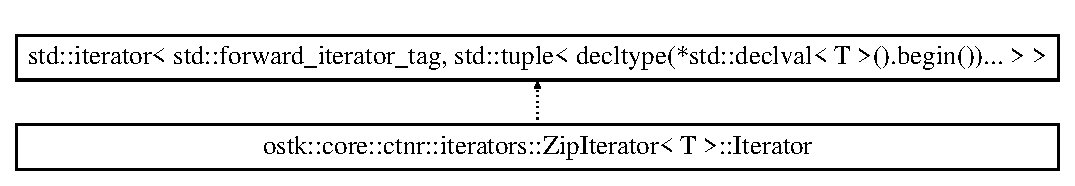
\includegraphics[height=2.000000cm]{classostk_1_1core_1_1ctnr_1_1iterators_1_1_zip_iterator_1_1_iterator}
\end{center}
\end{figure}
\subsection*{Public Member Functions}
\begin{DoxyCompactItemize}
\item 
\hyperlink{classostk_1_1core_1_1ctnr_1_1iterators_1_1_zip_iterator_1_1_iterator_acedc2e5184ab630d05c1b787c9052d50}{Iterator} (decltype(\hyperlink{classostk_1_1core_1_1ctnr_1_1iterators_1_1_zip_iterator_1_1_iterator_a37f6521fb9d0c8ec3ab94c56c06dd475}{iterators\+\_\+}) an\+Iterator\+List)
\item 
\hyperlink{classostk_1_1core_1_1ctnr_1_1iterators_1_1_zip_iterator_1_1_iterator}{Iterator} \& \hyperlink{classostk_1_1core_1_1ctnr_1_1iterators_1_1_zip_iterator_1_1_iterator_af6f0d0354e4f1a5e48b3d1e6671ed40d}{operator++} ()
\item 
\hyperlink{classostk_1_1core_1_1ctnr_1_1iterators_1_1_zip_iterator_1_1_iterator}{Iterator} \hyperlink{classostk_1_1core_1_1ctnr_1_1iterators_1_1_zip_iterator_1_1_iterator_adfe6573d7cb46ee10ee933521777719d}{operator++} (int)
\item 
bool \hyperlink{classostk_1_1core_1_1ctnr_1_1iterators_1_1_zip_iterator_1_1_iterator_abebad80eb725d8770ca4fd907aeaff25}{operator!=} (const \hyperlink{classostk_1_1core_1_1ctnr_1_1iterators_1_1_zip_iterator_1_1_iterator}{Iterator} \&an\+Iterator) const
\item 
auto \hyperlink{classostk_1_1core_1_1ctnr_1_1iterators_1_1_zip_iterator_1_1_iterator_a3a1cfa88cd06763edeaeffadea4740c5}{operator$\ast$} () const
\end{DoxyCompactItemize}
\subsection*{Public Attributes}
\begin{DoxyCompactItemize}
\item 
std\+::tuple$<$ decltype(std\+::declval$<$ T $>$).\hyperlink{classostk_1_1core_1_1ctnr_1_1iterators_1_1_zip_iterator_a9fd76a0b2306f00757c5a09accef725a}{begin}())... $>$ \hyperlink{classostk_1_1core_1_1ctnr_1_1iterators_1_1_zip_iterator_1_1_iterator_a37f6521fb9d0c8ec3ab94c56c06dd475}{iterators\+\_\+}
\end{DoxyCompactItemize}


\subsection{Constructor \& Destructor Documentation}
\mbox{\Hypertarget{classostk_1_1core_1_1ctnr_1_1iterators_1_1_zip_iterator_1_1_iterator_acedc2e5184ab630d05c1b787c9052d50}\label{classostk_1_1core_1_1ctnr_1_1iterators_1_1_zip_iterator_1_1_iterator_acedc2e5184ab630d05c1b787c9052d50}} 
\index{ostk\+::core\+::ctnr\+::iterators\+::\+Zip\+Iterator\+::\+Iterator@{ostk\+::core\+::ctnr\+::iterators\+::\+Zip\+Iterator\+::\+Iterator}!Iterator@{Iterator}}
\index{Iterator@{Iterator}!ostk\+::core\+::ctnr\+::iterators\+::\+Zip\+Iterator\+::\+Iterator@{ostk\+::core\+::ctnr\+::iterators\+::\+Zip\+Iterator\+::\+Iterator}}
\subsubsection{\texorpdfstring{Iterator()}{Iterator()}}
{\footnotesize\ttfamily template$<$typename... T$>$ \\
\hyperlink{classostk_1_1core_1_1ctnr_1_1iterators_1_1_zip_iterator}{ostk\+::core\+::ctnr\+::iterators\+::\+Zip\+Iterator}$<$ T $>$\+::Iterator\+::\+Iterator (\begin{DoxyParamCaption}\item[{decltype(\hyperlink{classostk_1_1core_1_1ctnr_1_1iterators_1_1_zip_iterator_1_1_iterator_a37f6521fb9d0c8ec3ab94c56c06dd475}{iterators\+\_\+})}]{an\+Iterator\+List }\end{DoxyParamCaption})\hspace{0.3cm}{\ttfamily [inline]}, {\ttfamily [explicit]}}



\subsection{Member Function Documentation}
\mbox{\Hypertarget{classostk_1_1core_1_1ctnr_1_1iterators_1_1_zip_iterator_1_1_iterator_abebad80eb725d8770ca4fd907aeaff25}\label{classostk_1_1core_1_1ctnr_1_1iterators_1_1_zip_iterator_1_1_iterator_abebad80eb725d8770ca4fd907aeaff25}} 
\index{ostk\+::core\+::ctnr\+::iterators\+::\+Zip\+Iterator\+::\+Iterator@{ostk\+::core\+::ctnr\+::iterators\+::\+Zip\+Iterator\+::\+Iterator}!operator"!=@{operator"!=}}
\index{operator"!=@{operator"!=}!ostk\+::core\+::ctnr\+::iterators\+::\+Zip\+Iterator\+::\+Iterator@{ostk\+::core\+::ctnr\+::iterators\+::\+Zip\+Iterator\+::\+Iterator}}
\subsubsection{\texorpdfstring{operator"!=()}{operator!=()}}
{\footnotesize\ttfamily template$<$typename... T$>$ \\
bool \hyperlink{classostk_1_1core_1_1ctnr_1_1iterators_1_1_zip_iterator}{ostk\+::core\+::ctnr\+::iterators\+::\+Zip\+Iterator}$<$ T $>$\+::Iterator\+::operator!= (\begin{DoxyParamCaption}\item[{const \hyperlink{classostk_1_1core_1_1ctnr_1_1iterators_1_1_zip_iterator_1_1_iterator}{Iterator} \&}]{an\+Iterator }\end{DoxyParamCaption}) const\hspace{0.3cm}{\ttfamily [inline]}}

\mbox{\Hypertarget{classostk_1_1core_1_1ctnr_1_1iterators_1_1_zip_iterator_1_1_iterator_a3a1cfa88cd06763edeaeffadea4740c5}\label{classostk_1_1core_1_1ctnr_1_1iterators_1_1_zip_iterator_1_1_iterator_a3a1cfa88cd06763edeaeffadea4740c5}} 
\index{ostk\+::core\+::ctnr\+::iterators\+::\+Zip\+Iterator\+::\+Iterator@{ostk\+::core\+::ctnr\+::iterators\+::\+Zip\+Iterator\+::\+Iterator}!operator$\ast$@{operator$\ast$}}
\index{operator$\ast$@{operator$\ast$}!ostk\+::core\+::ctnr\+::iterators\+::\+Zip\+Iterator\+::\+Iterator@{ostk\+::core\+::ctnr\+::iterators\+::\+Zip\+Iterator\+::\+Iterator}}
\subsubsection{\texorpdfstring{operator$\ast$()}{operator*()}}
{\footnotesize\ttfamily template$<$typename... T$>$ \\
auto \hyperlink{classostk_1_1core_1_1ctnr_1_1iterators_1_1_zip_iterator}{ostk\+::core\+::ctnr\+::iterators\+::\+Zip\+Iterator}$<$ T $>$\+::Iterator\+::operator$\ast$ (\begin{DoxyParamCaption}{ }\end{DoxyParamCaption}) const\hspace{0.3cm}{\ttfamily [inline]}}

\mbox{\Hypertarget{classostk_1_1core_1_1ctnr_1_1iterators_1_1_zip_iterator_1_1_iterator_af6f0d0354e4f1a5e48b3d1e6671ed40d}\label{classostk_1_1core_1_1ctnr_1_1iterators_1_1_zip_iterator_1_1_iterator_af6f0d0354e4f1a5e48b3d1e6671ed40d}} 
\index{ostk\+::core\+::ctnr\+::iterators\+::\+Zip\+Iterator\+::\+Iterator@{ostk\+::core\+::ctnr\+::iterators\+::\+Zip\+Iterator\+::\+Iterator}!operator++@{operator++}}
\index{operator++@{operator++}!ostk\+::core\+::ctnr\+::iterators\+::\+Zip\+Iterator\+::\+Iterator@{ostk\+::core\+::ctnr\+::iterators\+::\+Zip\+Iterator\+::\+Iterator}}
\subsubsection{\texorpdfstring{operator++()}{operator++()}\hspace{0.1cm}{\footnotesize\ttfamily [1/2]}}
{\footnotesize\ttfamily template$<$typename... T$>$ \\
\hyperlink{classostk_1_1core_1_1ctnr_1_1iterators_1_1_zip_iterator_1_1_iterator}{Iterator}\& \hyperlink{classostk_1_1core_1_1ctnr_1_1iterators_1_1_zip_iterator}{ostk\+::core\+::ctnr\+::iterators\+::\+Zip\+Iterator}$<$ T $>$\+::Iterator\+::operator++ (\begin{DoxyParamCaption}{ }\end{DoxyParamCaption})\hspace{0.3cm}{\ttfamily [inline]}}

\mbox{\Hypertarget{classostk_1_1core_1_1ctnr_1_1iterators_1_1_zip_iterator_1_1_iterator_adfe6573d7cb46ee10ee933521777719d}\label{classostk_1_1core_1_1ctnr_1_1iterators_1_1_zip_iterator_1_1_iterator_adfe6573d7cb46ee10ee933521777719d}} 
\index{ostk\+::core\+::ctnr\+::iterators\+::\+Zip\+Iterator\+::\+Iterator@{ostk\+::core\+::ctnr\+::iterators\+::\+Zip\+Iterator\+::\+Iterator}!operator++@{operator++}}
\index{operator++@{operator++}!ostk\+::core\+::ctnr\+::iterators\+::\+Zip\+Iterator\+::\+Iterator@{ostk\+::core\+::ctnr\+::iterators\+::\+Zip\+Iterator\+::\+Iterator}}
\subsubsection{\texorpdfstring{operator++()}{operator++()}\hspace{0.1cm}{\footnotesize\ttfamily [2/2]}}
{\footnotesize\ttfamily template$<$typename... T$>$ \\
\hyperlink{classostk_1_1core_1_1ctnr_1_1iterators_1_1_zip_iterator_1_1_iterator}{Iterator} \hyperlink{classostk_1_1core_1_1ctnr_1_1iterators_1_1_zip_iterator}{ostk\+::core\+::ctnr\+::iterators\+::\+Zip\+Iterator}$<$ T $>$\+::Iterator\+::operator++ (\begin{DoxyParamCaption}\item[{int}]{ }\end{DoxyParamCaption})\hspace{0.3cm}{\ttfamily [inline]}}



\subsection{Member Data Documentation}
\mbox{\Hypertarget{classostk_1_1core_1_1ctnr_1_1iterators_1_1_zip_iterator_1_1_iterator_a37f6521fb9d0c8ec3ab94c56c06dd475}\label{classostk_1_1core_1_1ctnr_1_1iterators_1_1_zip_iterator_1_1_iterator_a37f6521fb9d0c8ec3ab94c56c06dd475}} 
\index{ostk\+::core\+::ctnr\+::iterators\+::\+Zip\+Iterator\+::\+Iterator@{ostk\+::core\+::ctnr\+::iterators\+::\+Zip\+Iterator\+::\+Iterator}!iterators\+\_\+@{iterators\+\_\+}}
\index{iterators\+\_\+@{iterators\+\_\+}!ostk\+::core\+::ctnr\+::iterators\+::\+Zip\+Iterator\+::\+Iterator@{ostk\+::core\+::ctnr\+::iterators\+::\+Zip\+Iterator\+::\+Iterator}}
\subsubsection{\texorpdfstring{iterators\+\_\+}{iterators\_}}
{\footnotesize\ttfamily template$<$typename... T$>$ \\
std\+::tuple$<$decltype(std\+::declval$<$T$>$).\hyperlink{classostk_1_1core_1_1ctnr_1_1iterators_1_1_zip_iterator_a9fd76a0b2306f00757c5a09accef725a}{begin}())...$>$ \hyperlink{classostk_1_1core_1_1ctnr_1_1iterators_1_1_zip_iterator}{ostk\+::core\+::ctnr\+::iterators\+::\+Zip\+Iterator}$<$ T $>$\+::Iterator\+::iterators\+\_\+}



The documentation for this class was generated from the following file\+:\begin{DoxyCompactItemize}
\item 
include/\+Open\+Space\+Toolkit/\+Core/\+Containers/\+Iterators/\hyperlink{_zip_8hpp}{Zip.\+hpp}\end{DoxyCompactItemize}

\hypertarget{classostk_1_1core_1_1ctnr_1_1_dictionary_1_1_iterator}{}\section{ostk\+:\+:core\+:\+:ctnr\+:\+:Dictionary\+:\+:Iterator Class Reference}
\label{classostk_1_1core_1_1ctnr_1_1_dictionary_1_1_iterator}\index{ostk\+::core\+::ctnr\+::\+Dictionary\+::\+Iterator@{ostk\+::core\+::ctnr\+::\+Dictionary\+::\+Iterator}}


{\ttfamily \#include $<$Dictionary.\+hpp$>$}

\subsection*{Public Types}
\begin{DoxyCompactItemize}
\item 
typedef \hyperlink{namespaceostk_1_1core_1_1ctnr_a13ac23065e75eb425f38bfca4d0c6b38}{Ordered\+Map}$<$ \hyperlink{classostk_1_1core_1_1ctnr_1_1_dictionary_aa3b171525039535f342d271d27f90407}{Dictionary\+::\+Key}, \hyperlink{classostk_1_1core_1_1ctnr_1_1_dictionary_ace6ab82268031e972455affca8730c9c}{Dictionary\+::\+Value} $>$\+::iterator \hyperlink{classostk_1_1core_1_1ctnr_1_1_dictionary_1_1_iterator_a0d5a95dd4a931ded2d8d156da4499348}{Map\+Iterator}
\end{DoxyCompactItemize}
\subsection*{Public Member Functions}
\begin{DoxyCompactItemize}
\item 
\hyperlink{classostk_1_1core_1_1ctnr_1_1_dictionary_1_1_iterator_a072bec9bfbccbebddaf07b8ed5464342}{Iterator} ()
\item 
\hyperlink{classostk_1_1core_1_1ctnr_1_1_dictionary_1_1_iterator_a00b1067c55db4dc369028196f80b1f2c}{Iterator} (const \hyperlink{classostk_1_1core_1_1ctnr_1_1_dictionary_1_1_iterator_a0d5a95dd4a931ded2d8d156da4499348}{Iterator\+::\+Map\+Iterator} \&an\+Ordered\+Map\+It)
\item 
\hyperlink{classostk_1_1core_1_1ctnr_1_1_dictionary_1_1_iterator_a9d5eeb27e91c5c6907c106b71c4fa0a7}{Iterator} (const \hyperlink{classostk_1_1core_1_1ctnr_1_1_dictionary_1_1_iterator}{Iterator} \&a\+Iterator)
\item 
\hyperlink{classostk_1_1core_1_1ctnr_1_1_dictionary_1_1_iterator}{Iterator} \& \hyperlink{classostk_1_1core_1_1ctnr_1_1_dictionary_1_1_iterator_a18334755781a37f30c9a9e6769154154}{operator=} (const \hyperlink{classostk_1_1core_1_1ctnr_1_1_dictionary_1_1_iterator}{Iterator} \&a\+Iterator)
\item 
bool \hyperlink{classostk_1_1core_1_1ctnr_1_1_dictionary_1_1_iterator_a255e6f3e13f9409a4e6cb9bbec6a48b7}{operator==} (const \hyperlink{classostk_1_1core_1_1ctnr_1_1_dictionary_1_1_iterator}{Iterator} \&a\+Iterator) const
\item 
bool \hyperlink{classostk_1_1core_1_1ctnr_1_1_dictionary_1_1_iterator_a6bff7f1ddeef729f87725848647fd662}{operator!=} (const \hyperlink{classostk_1_1core_1_1ctnr_1_1_dictionary_1_1_iterator}{Iterator} \&a\+Iterator) const
\item 
const \hyperlink{classostk_1_1core_1_1ctnr_1_1_dictionary_1_1_iterator}{Iterator} \& \hyperlink{classostk_1_1core_1_1ctnr_1_1_dictionary_1_1_iterator_a4dbb071ffe9ecb5ec238f54fe8ef25c2}{operator$\ast$} () const
\item 
const \hyperlink{classostk_1_1core_1_1ctnr_1_1_dictionary_1_1_iterator}{Iterator} $\ast$ \hyperlink{classostk_1_1core_1_1ctnr_1_1_dictionary_1_1_iterator_af11668451d7a7da9442a54c820a37666}{operator-\/$>$} () const
\item 
\hyperlink{classostk_1_1core_1_1ctnr_1_1_dictionary_1_1_iterator}{Iterator} \& \hyperlink{classostk_1_1core_1_1ctnr_1_1_dictionary_1_1_iterator_a170f805b2ecf85c1e30cfbe7af43d95f}{operator$\ast$} ()
\item 
\hyperlink{classostk_1_1core_1_1ctnr_1_1_dictionary_1_1_iterator}{Iterator} $\ast$ \hyperlink{classostk_1_1core_1_1ctnr_1_1_dictionary_1_1_iterator_ab5332606378259f3eca841295f962c50}{operator-\/$>$} ()
\item 
\hyperlink{classostk_1_1core_1_1ctnr_1_1_dictionary_ace6ab82268031e972455affca8730c9c}{Dictionary\+::\+Value} \& \hyperlink{classostk_1_1core_1_1ctnr_1_1_dictionary_1_1_iterator_a9bd8822700f2d7faf1a9aa5df834ebcf}{operator\mbox{[}$\,$\mbox{]}} (const \hyperlink{classostk_1_1core_1_1ctnr_1_1_dictionary_aa3b171525039535f342d271d27f90407}{Dictionary\+::\+Key} \&a\+Key)
\item 
\hyperlink{classostk_1_1core_1_1ctnr_1_1_dictionary_1_1_iterator}{Iterator} \& \hyperlink{classostk_1_1core_1_1ctnr_1_1_dictionary_1_1_iterator_adf30c71ce87d20e5121816529b74ad7c}{operator++} ()
\item 
\hyperlink{classostk_1_1core_1_1ctnr_1_1_dictionary_1_1_iterator}{Iterator} \hyperlink{classostk_1_1core_1_1ctnr_1_1_dictionary_1_1_iterator_a88d93addbb00f5be55b99f9191149497}{operator++} (int)
\item 
\hyperlink{classostk_1_1core_1_1ctnr_1_1_dictionary_1_1_iterator}{Iterator} \& \hyperlink{classostk_1_1core_1_1ctnr_1_1_dictionary_1_1_iterator_a19678c493ef740431484ea4c83bbc65b}{operator-\/-\/} ()
\item 
\hyperlink{classostk_1_1core_1_1ctnr_1_1_dictionary_1_1_iterator}{Iterator} \hyperlink{classostk_1_1core_1_1ctnr_1_1_dictionary_1_1_iterator_a6e2e6ce5737aa845fdc0300f962ac74c}{operator-\/-\/} (int)
\item 
const \hyperlink{classostk_1_1core_1_1ctnr_1_1_dictionary_aa3b171525039535f342d271d27f90407}{Dictionary\+::\+Key} \& \hyperlink{classostk_1_1core_1_1ctnr_1_1_dictionary_1_1_iterator_a80efd995a416d7285fa9f44954fc4297}{access\+Key} () const
\item 
const \hyperlink{classostk_1_1core_1_1ctnr_1_1_dictionary_ace6ab82268031e972455affca8730c9c}{Dictionary\+::\+Value} \& \hyperlink{classostk_1_1core_1_1ctnr_1_1_dictionary_1_1_iterator_ac8061d68101441f2c8aa855736047060}{access\+Value} () const
\item 
\hyperlink{classostk_1_1core_1_1ctnr_1_1_dictionary_ace6ab82268031e972455affca8730c9c}{Dictionary\+::\+Value} \& \hyperlink{classostk_1_1core_1_1ctnr_1_1_dictionary_1_1_iterator_a16034f95ffc39b5a89d6d699a5964e1f}{access\+Value} ()
\item 
const \hyperlink{classostk_1_1core_1_1ctnr_1_1_dictionary_1_1_iterator_a0d5a95dd4a931ded2d8d156da4499348}{Iterator\+::\+Map\+Iterator} \& \hyperlink{classostk_1_1core_1_1ctnr_1_1_dictionary_1_1_iterator_a578bb7a0d61c11f6a43ff9e67448707f}{access\+Map\+Iterator} () const
\item 
\hyperlink{classostk_1_1core_1_1ctnr_1_1_dictionary_1_1_iterator_a0d5a95dd4a931ded2d8d156da4499348}{Iterator\+::\+Map\+Iterator} \& \hyperlink{classostk_1_1core_1_1ctnr_1_1_dictionary_1_1_iterator_abbd4e8107ae7f7c56f2b26a67552fd0d}{access\+Map\+Iterator} ()
\end{DoxyCompactItemize}


\subsection{Member Typedef Documentation}
\mbox{\Hypertarget{classostk_1_1core_1_1ctnr_1_1_dictionary_1_1_iterator_a0d5a95dd4a931ded2d8d156da4499348}\label{classostk_1_1core_1_1ctnr_1_1_dictionary_1_1_iterator_a0d5a95dd4a931ded2d8d156da4499348}} 
\index{ostk\+::core\+::ctnr\+::\+Dictionary\+::\+Iterator@{ostk\+::core\+::ctnr\+::\+Dictionary\+::\+Iterator}!Map\+Iterator@{Map\+Iterator}}
\index{Map\+Iterator@{Map\+Iterator}!ostk\+::core\+::ctnr\+::\+Dictionary\+::\+Iterator@{ostk\+::core\+::ctnr\+::\+Dictionary\+::\+Iterator}}
\subsubsection{\texorpdfstring{Map\+Iterator}{MapIterator}}
{\footnotesize\ttfamily typedef \hyperlink{namespaceostk_1_1core_1_1ctnr_a13ac23065e75eb425f38bfca4d0c6b38}{Ordered\+Map}$<$\hyperlink{classostk_1_1core_1_1ctnr_1_1_dictionary_aa3b171525039535f342d271d27f90407}{Dictionary\+::\+Key}, \hyperlink{classostk_1_1core_1_1ctnr_1_1_dictionary_ace6ab82268031e972455affca8730c9c}{Dictionary\+::\+Value}$>$\+::iterator \hyperlink{classostk_1_1core_1_1ctnr_1_1_dictionary_1_1_iterator_a0d5a95dd4a931ded2d8d156da4499348}{ostk\+::core\+::ctnr\+::\+Dictionary\+::\+Iterator\+::\+Map\+Iterator}}



\subsection{Constructor \& Destructor Documentation}
\mbox{\Hypertarget{classostk_1_1core_1_1ctnr_1_1_dictionary_1_1_iterator_a072bec9bfbccbebddaf07b8ed5464342}\label{classostk_1_1core_1_1ctnr_1_1_dictionary_1_1_iterator_a072bec9bfbccbebddaf07b8ed5464342}} 
\index{ostk\+::core\+::ctnr\+::\+Dictionary\+::\+Iterator@{ostk\+::core\+::ctnr\+::\+Dictionary\+::\+Iterator}!Iterator@{Iterator}}
\index{Iterator@{Iterator}!ostk\+::core\+::ctnr\+::\+Dictionary\+::\+Iterator@{ostk\+::core\+::ctnr\+::\+Dictionary\+::\+Iterator}}
\subsubsection{\texorpdfstring{Iterator()}{Iterator()}\hspace{0.1cm}{\footnotesize\ttfamily [1/3]}}
{\footnotesize\ttfamily ostk\+::core\+::ctnr\+::\+Dictionary\+::\+Iterator\+::\+Iterator (\begin{DoxyParamCaption}{ }\end{DoxyParamCaption})}

\mbox{\Hypertarget{classostk_1_1core_1_1ctnr_1_1_dictionary_1_1_iterator_a00b1067c55db4dc369028196f80b1f2c}\label{classostk_1_1core_1_1ctnr_1_1_dictionary_1_1_iterator_a00b1067c55db4dc369028196f80b1f2c}} 
\index{ostk\+::core\+::ctnr\+::\+Dictionary\+::\+Iterator@{ostk\+::core\+::ctnr\+::\+Dictionary\+::\+Iterator}!Iterator@{Iterator}}
\index{Iterator@{Iterator}!ostk\+::core\+::ctnr\+::\+Dictionary\+::\+Iterator@{ostk\+::core\+::ctnr\+::\+Dictionary\+::\+Iterator}}
\subsubsection{\texorpdfstring{Iterator()}{Iterator()}\hspace{0.1cm}{\footnotesize\ttfamily [2/3]}}
{\footnotesize\ttfamily ostk\+::core\+::ctnr\+::\+Dictionary\+::\+Iterator\+::\+Iterator (\begin{DoxyParamCaption}\item[{const \hyperlink{classostk_1_1core_1_1ctnr_1_1_dictionary_1_1_iterator_a0d5a95dd4a931ded2d8d156da4499348}{Iterator\+::\+Map\+Iterator} \&}]{an\+Ordered\+Map\+It }\end{DoxyParamCaption})}

\mbox{\Hypertarget{classostk_1_1core_1_1ctnr_1_1_dictionary_1_1_iterator_a9d5eeb27e91c5c6907c106b71c4fa0a7}\label{classostk_1_1core_1_1ctnr_1_1_dictionary_1_1_iterator_a9d5eeb27e91c5c6907c106b71c4fa0a7}} 
\index{ostk\+::core\+::ctnr\+::\+Dictionary\+::\+Iterator@{ostk\+::core\+::ctnr\+::\+Dictionary\+::\+Iterator}!Iterator@{Iterator}}
\index{Iterator@{Iterator}!ostk\+::core\+::ctnr\+::\+Dictionary\+::\+Iterator@{ostk\+::core\+::ctnr\+::\+Dictionary\+::\+Iterator}}
\subsubsection{\texorpdfstring{Iterator()}{Iterator()}\hspace{0.1cm}{\footnotesize\ttfamily [3/3]}}
{\footnotesize\ttfamily ostk\+::core\+::ctnr\+::\+Dictionary\+::\+Iterator\+::\+Iterator (\begin{DoxyParamCaption}\item[{const \hyperlink{classostk_1_1core_1_1ctnr_1_1_dictionary_1_1_iterator}{Iterator} \&}]{a\+Iterator }\end{DoxyParamCaption})}



\subsection{Member Function Documentation}
\mbox{\Hypertarget{classostk_1_1core_1_1ctnr_1_1_dictionary_1_1_iterator_a80efd995a416d7285fa9f44954fc4297}\label{classostk_1_1core_1_1ctnr_1_1_dictionary_1_1_iterator_a80efd995a416d7285fa9f44954fc4297}} 
\index{ostk\+::core\+::ctnr\+::\+Dictionary\+::\+Iterator@{ostk\+::core\+::ctnr\+::\+Dictionary\+::\+Iterator}!access\+Key@{access\+Key}}
\index{access\+Key@{access\+Key}!ostk\+::core\+::ctnr\+::\+Dictionary\+::\+Iterator@{ostk\+::core\+::ctnr\+::\+Dictionary\+::\+Iterator}}
\subsubsection{\texorpdfstring{access\+Key()}{accessKey()}}
{\footnotesize\ttfamily const \hyperlink{classostk_1_1core_1_1ctnr_1_1_dictionary_aa3b171525039535f342d271d27f90407}{Dictionary\+::\+Key} \& ostk\+::core\+::ctnr\+::\+Dictionary\+::\+Iterator\+::access\+Key (\begin{DoxyParamCaption}{ }\end{DoxyParamCaption}) const}

\mbox{\Hypertarget{classostk_1_1core_1_1ctnr_1_1_dictionary_1_1_iterator_a578bb7a0d61c11f6a43ff9e67448707f}\label{classostk_1_1core_1_1ctnr_1_1_dictionary_1_1_iterator_a578bb7a0d61c11f6a43ff9e67448707f}} 
\index{ostk\+::core\+::ctnr\+::\+Dictionary\+::\+Iterator@{ostk\+::core\+::ctnr\+::\+Dictionary\+::\+Iterator}!access\+Map\+Iterator@{access\+Map\+Iterator}}
\index{access\+Map\+Iterator@{access\+Map\+Iterator}!ostk\+::core\+::ctnr\+::\+Dictionary\+::\+Iterator@{ostk\+::core\+::ctnr\+::\+Dictionary\+::\+Iterator}}
\subsubsection{\texorpdfstring{access\+Map\+Iterator()}{accessMapIterator()}\hspace{0.1cm}{\footnotesize\ttfamily [1/2]}}
{\footnotesize\ttfamily const \hyperlink{classostk_1_1core_1_1ctnr_1_1_dictionary_1_1_iterator_a0d5a95dd4a931ded2d8d156da4499348}{Dictionary\+::\+Iterator\+::\+Map\+Iterator} \& ostk\+::core\+::ctnr\+::\+Dictionary\+::\+Iterator\+::access\+Map\+Iterator (\begin{DoxyParamCaption}{ }\end{DoxyParamCaption}) const}

\mbox{\Hypertarget{classostk_1_1core_1_1ctnr_1_1_dictionary_1_1_iterator_abbd4e8107ae7f7c56f2b26a67552fd0d}\label{classostk_1_1core_1_1ctnr_1_1_dictionary_1_1_iterator_abbd4e8107ae7f7c56f2b26a67552fd0d}} 
\index{ostk\+::core\+::ctnr\+::\+Dictionary\+::\+Iterator@{ostk\+::core\+::ctnr\+::\+Dictionary\+::\+Iterator}!access\+Map\+Iterator@{access\+Map\+Iterator}}
\index{access\+Map\+Iterator@{access\+Map\+Iterator}!ostk\+::core\+::ctnr\+::\+Dictionary\+::\+Iterator@{ostk\+::core\+::ctnr\+::\+Dictionary\+::\+Iterator}}
\subsubsection{\texorpdfstring{access\+Map\+Iterator()}{accessMapIterator()}\hspace{0.1cm}{\footnotesize\ttfamily [2/2]}}
{\footnotesize\ttfamily \hyperlink{classostk_1_1core_1_1ctnr_1_1_dictionary_1_1_iterator_a0d5a95dd4a931ded2d8d156da4499348}{Dictionary\+::\+Iterator\+::\+Map\+Iterator} \& ostk\+::core\+::ctnr\+::\+Dictionary\+::\+Iterator\+::access\+Map\+Iterator (\begin{DoxyParamCaption}{ }\end{DoxyParamCaption})}

\mbox{\Hypertarget{classostk_1_1core_1_1ctnr_1_1_dictionary_1_1_iterator_ac8061d68101441f2c8aa855736047060}\label{classostk_1_1core_1_1ctnr_1_1_dictionary_1_1_iterator_ac8061d68101441f2c8aa855736047060}} 
\index{ostk\+::core\+::ctnr\+::\+Dictionary\+::\+Iterator@{ostk\+::core\+::ctnr\+::\+Dictionary\+::\+Iterator}!access\+Value@{access\+Value}}
\index{access\+Value@{access\+Value}!ostk\+::core\+::ctnr\+::\+Dictionary\+::\+Iterator@{ostk\+::core\+::ctnr\+::\+Dictionary\+::\+Iterator}}
\subsubsection{\texorpdfstring{access\+Value()}{accessValue()}\hspace{0.1cm}{\footnotesize\ttfamily [1/2]}}
{\footnotesize\ttfamily const \hyperlink{classostk_1_1core_1_1ctnr_1_1_dictionary_ace6ab82268031e972455affca8730c9c}{Dictionary\+::\+Value} \& ostk\+::core\+::ctnr\+::\+Dictionary\+::\+Iterator\+::access\+Value (\begin{DoxyParamCaption}{ }\end{DoxyParamCaption}) const}

\mbox{\Hypertarget{classostk_1_1core_1_1ctnr_1_1_dictionary_1_1_iterator_a16034f95ffc39b5a89d6d699a5964e1f}\label{classostk_1_1core_1_1ctnr_1_1_dictionary_1_1_iterator_a16034f95ffc39b5a89d6d699a5964e1f}} 
\index{ostk\+::core\+::ctnr\+::\+Dictionary\+::\+Iterator@{ostk\+::core\+::ctnr\+::\+Dictionary\+::\+Iterator}!access\+Value@{access\+Value}}
\index{access\+Value@{access\+Value}!ostk\+::core\+::ctnr\+::\+Dictionary\+::\+Iterator@{ostk\+::core\+::ctnr\+::\+Dictionary\+::\+Iterator}}
\subsubsection{\texorpdfstring{access\+Value()}{accessValue()}\hspace{0.1cm}{\footnotesize\ttfamily [2/2]}}
{\footnotesize\ttfamily \hyperlink{classostk_1_1core_1_1ctnr_1_1_dictionary_ace6ab82268031e972455affca8730c9c}{Dictionary\+::\+Value} \& ostk\+::core\+::ctnr\+::\+Dictionary\+::\+Iterator\+::access\+Value (\begin{DoxyParamCaption}{ }\end{DoxyParamCaption})}

\mbox{\Hypertarget{classostk_1_1core_1_1ctnr_1_1_dictionary_1_1_iterator_a6bff7f1ddeef729f87725848647fd662}\label{classostk_1_1core_1_1ctnr_1_1_dictionary_1_1_iterator_a6bff7f1ddeef729f87725848647fd662}} 
\index{ostk\+::core\+::ctnr\+::\+Dictionary\+::\+Iterator@{ostk\+::core\+::ctnr\+::\+Dictionary\+::\+Iterator}!operator"!=@{operator"!=}}
\index{operator"!=@{operator"!=}!ostk\+::core\+::ctnr\+::\+Dictionary\+::\+Iterator@{ostk\+::core\+::ctnr\+::\+Dictionary\+::\+Iterator}}
\subsubsection{\texorpdfstring{operator"!=()}{operator!=()}}
{\footnotesize\ttfamily bool ostk\+::core\+::ctnr\+::\+Dictionary\+::\+Iterator\+::operator!= (\begin{DoxyParamCaption}\item[{const \hyperlink{classostk_1_1core_1_1ctnr_1_1_dictionary_1_1_iterator}{Iterator} \&}]{a\+Iterator }\end{DoxyParamCaption}) const}

\mbox{\Hypertarget{classostk_1_1core_1_1ctnr_1_1_dictionary_1_1_iterator_a4dbb071ffe9ecb5ec238f54fe8ef25c2}\label{classostk_1_1core_1_1ctnr_1_1_dictionary_1_1_iterator_a4dbb071ffe9ecb5ec238f54fe8ef25c2}} 
\index{ostk\+::core\+::ctnr\+::\+Dictionary\+::\+Iterator@{ostk\+::core\+::ctnr\+::\+Dictionary\+::\+Iterator}!operator$\ast$@{operator$\ast$}}
\index{operator$\ast$@{operator$\ast$}!ostk\+::core\+::ctnr\+::\+Dictionary\+::\+Iterator@{ostk\+::core\+::ctnr\+::\+Dictionary\+::\+Iterator}}
\subsubsection{\texorpdfstring{operator$\ast$()}{operator*()}\hspace{0.1cm}{\footnotesize\ttfamily [1/2]}}
{\footnotesize\ttfamily const \hyperlink{classostk_1_1core_1_1ctnr_1_1_dictionary_1_1_iterator}{Dictionary\+::\+Iterator} \& ostk\+::core\+::ctnr\+::\+Dictionary\+::\+Iterator\+::operator$\ast$ (\begin{DoxyParamCaption}{ }\end{DoxyParamCaption}) const}

\mbox{\Hypertarget{classostk_1_1core_1_1ctnr_1_1_dictionary_1_1_iterator_a170f805b2ecf85c1e30cfbe7af43d95f}\label{classostk_1_1core_1_1ctnr_1_1_dictionary_1_1_iterator_a170f805b2ecf85c1e30cfbe7af43d95f}} 
\index{ostk\+::core\+::ctnr\+::\+Dictionary\+::\+Iterator@{ostk\+::core\+::ctnr\+::\+Dictionary\+::\+Iterator}!operator$\ast$@{operator$\ast$}}
\index{operator$\ast$@{operator$\ast$}!ostk\+::core\+::ctnr\+::\+Dictionary\+::\+Iterator@{ostk\+::core\+::ctnr\+::\+Dictionary\+::\+Iterator}}
\subsubsection{\texorpdfstring{operator$\ast$()}{operator*()}\hspace{0.1cm}{\footnotesize\ttfamily [2/2]}}
{\footnotesize\ttfamily \hyperlink{classostk_1_1core_1_1ctnr_1_1_dictionary_1_1_iterator}{Dictionary\+::\+Iterator} \& ostk\+::core\+::ctnr\+::\+Dictionary\+::\+Iterator\+::operator$\ast$ (\begin{DoxyParamCaption}{ }\end{DoxyParamCaption})}

\mbox{\Hypertarget{classostk_1_1core_1_1ctnr_1_1_dictionary_1_1_iterator_adf30c71ce87d20e5121816529b74ad7c}\label{classostk_1_1core_1_1ctnr_1_1_dictionary_1_1_iterator_adf30c71ce87d20e5121816529b74ad7c}} 
\index{ostk\+::core\+::ctnr\+::\+Dictionary\+::\+Iterator@{ostk\+::core\+::ctnr\+::\+Dictionary\+::\+Iterator}!operator++@{operator++}}
\index{operator++@{operator++}!ostk\+::core\+::ctnr\+::\+Dictionary\+::\+Iterator@{ostk\+::core\+::ctnr\+::\+Dictionary\+::\+Iterator}}
\subsubsection{\texorpdfstring{operator++()}{operator++()}\hspace{0.1cm}{\footnotesize\ttfamily [1/2]}}
{\footnotesize\ttfamily \hyperlink{classostk_1_1core_1_1ctnr_1_1_dictionary_1_1_iterator}{Dictionary\+::\+Iterator} \& ostk\+::core\+::ctnr\+::\+Dictionary\+::\+Iterator\+::operator++ (\begin{DoxyParamCaption}{ }\end{DoxyParamCaption})}

\mbox{\Hypertarget{classostk_1_1core_1_1ctnr_1_1_dictionary_1_1_iterator_a88d93addbb00f5be55b99f9191149497}\label{classostk_1_1core_1_1ctnr_1_1_dictionary_1_1_iterator_a88d93addbb00f5be55b99f9191149497}} 
\index{ostk\+::core\+::ctnr\+::\+Dictionary\+::\+Iterator@{ostk\+::core\+::ctnr\+::\+Dictionary\+::\+Iterator}!operator++@{operator++}}
\index{operator++@{operator++}!ostk\+::core\+::ctnr\+::\+Dictionary\+::\+Iterator@{ostk\+::core\+::ctnr\+::\+Dictionary\+::\+Iterator}}
\subsubsection{\texorpdfstring{operator++()}{operator++()}\hspace{0.1cm}{\footnotesize\ttfamily [2/2]}}
{\footnotesize\ttfamily \hyperlink{classostk_1_1core_1_1ctnr_1_1_dictionary_1_1_iterator}{Dictionary\+::\+Iterator} ostk\+::core\+::ctnr\+::\+Dictionary\+::\+Iterator\+::operator++ (\begin{DoxyParamCaption}\item[{int}]{ }\end{DoxyParamCaption})}

\mbox{\Hypertarget{classostk_1_1core_1_1ctnr_1_1_dictionary_1_1_iterator_a19678c493ef740431484ea4c83bbc65b}\label{classostk_1_1core_1_1ctnr_1_1_dictionary_1_1_iterator_a19678c493ef740431484ea4c83bbc65b}} 
\index{ostk\+::core\+::ctnr\+::\+Dictionary\+::\+Iterator@{ostk\+::core\+::ctnr\+::\+Dictionary\+::\+Iterator}!operator-\/-\/@{operator-\/-\/}}
\index{operator-\/-\/@{operator-\/-\/}!ostk\+::core\+::ctnr\+::\+Dictionary\+::\+Iterator@{ostk\+::core\+::ctnr\+::\+Dictionary\+::\+Iterator}}
\subsubsection{\texorpdfstring{operator-\/-\/()}{operator--()}\hspace{0.1cm}{\footnotesize\ttfamily [1/2]}}
{\footnotesize\ttfamily \hyperlink{classostk_1_1core_1_1ctnr_1_1_dictionary_1_1_iterator}{Dictionary\+::\+Iterator} \& ostk\+::core\+::ctnr\+::\+Dictionary\+::\+Iterator\+::operator-\/-\/ (\begin{DoxyParamCaption}{ }\end{DoxyParamCaption})}

\mbox{\Hypertarget{classostk_1_1core_1_1ctnr_1_1_dictionary_1_1_iterator_a6e2e6ce5737aa845fdc0300f962ac74c}\label{classostk_1_1core_1_1ctnr_1_1_dictionary_1_1_iterator_a6e2e6ce5737aa845fdc0300f962ac74c}} 
\index{ostk\+::core\+::ctnr\+::\+Dictionary\+::\+Iterator@{ostk\+::core\+::ctnr\+::\+Dictionary\+::\+Iterator}!operator-\/-\/@{operator-\/-\/}}
\index{operator-\/-\/@{operator-\/-\/}!ostk\+::core\+::ctnr\+::\+Dictionary\+::\+Iterator@{ostk\+::core\+::ctnr\+::\+Dictionary\+::\+Iterator}}
\subsubsection{\texorpdfstring{operator-\/-\/()}{operator--()}\hspace{0.1cm}{\footnotesize\ttfamily [2/2]}}
{\footnotesize\ttfamily \hyperlink{classostk_1_1core_1_1ctnr_1_1_dictionary_1_1_iterator}{Dictionary\+::\+Iterator} ostk\+::core\+::ctnr\+::\+Dictionary\+::\+Iterator\+::operator-\/-\/ (\begin{DoxyParamCaption}\item[{int}]{ }\end{DoxyParamCaption})}

\mbox{\Hypertarget{classostk_1_1core_1_1ctnr_1_1_dictionary_1_1_iterator_af11668451d7a7da9442a54c820a37666}\label{classostk_1_1core_1_1ctnr_1_1_dictionary_1_1_iterator_af11668451d7a7da9442a54c820a37666}} 
\index{ostk\+::core\+::ctnr\+::\+Dictionary\+::\+Iterator@{ostk\+::core\+::ctnr\+::\+Dictionary\+::\+Iterator}!operator-\/$>$@{operator-\/$>$}}
\index{operator-\/$>$@{operator-\/$>$}!ostk\+::core\+::ctnr\+::\+Dictionary\+::\+Iterator@{ostk\+::core\+::ctnr\+::\+Dictionary\+::\+Iterator}}
\subsubsection{\texorpdfstring{operator-\/$>$()}{operator->()}\hspace{0.1cm}{\footnotesize\ttfamily [1/2]}}
{\footnotesize\ttfamily const \hyperlink{classostk_1_1core_1_1ctnr_1_1_dictionary_1_1_iterator}{Dictionary\+::\+Iterator} $\ast$ ostk\+::core\+::ctnr\+::\+Dictionary\+::\+Iterator\+::operator-\/$>$ (\begin{DoxyParamCaption}{ }\end{DoxyParamCaption}) const}

\mbox{\Hypertarget{classostk_1_1core_1_1ctnr_1_1_dictionary_1_1_iterator_ab5332606378259f3eca841295f962c50}\label{classostk_1_1core_1_1ctnr_1_1_dictionary_1_1_iterator_ab5332606378259f3eca841295f962c50}} 
\index{ostk\+::core\+::ctnr\+::\+Dictionary\+::\+Iterator@{ostk\+::core\+::ctnr\+::\+Dictionary\+::\+Iterator}!operator-\/$>$@{operator-\/$>$}}
\index{operator-\/$>$@{operator-\/$>$}!ostk\+::core\+::ctnr\+::\+Dictionary\+::\+Iterator@{ostk\+::core\+::ctnr\+::\+Dictionary\+::\+Iterator}}
\subsubsection{\texorpdfstring{operator-\/$>$()}{operator->()}\hspace{0.1cm}{\footnotesize\ttfamily [2/2]}}
{\footnotesize\ttfamily \hyperlink{classostk_1_1core_1_1ctnr_1_1_dictionary_1_1_iterator}{Dictionary\+::\+Iterator} $\ast$ ostk\+::core\+::ctnr\+::\+Dictionary\+::\+Iterator\+::operator-\/$>$ (\begin{DoxyParamCaption}{ }\end{DoxyParamCaption})}

\mbox{\Hypertarget{classostk_1_1core_1_1ctnr_1_1_dictionary_1_1_iterator_a18334755781a37f30c9a9e6769154154}\label{classostk_1_1core_1_1ctnr_1_1_dictionary_1_1_iterator_a18334755781a37f30c9a9e6769154154}} 
\index{ostk\+::core\+::ctnr\+::\+Dictionary\+::\+Iterator@{ostk\+::core\+::ctnr\+::\+Dictionary\+::\+Iterator}!operator=@{operator=}}
\index{operator=@{operator=}!ostk\+::core\+::ctnr\+::\+Dictionary\+::\+Iterator@{ostk\+::core\+::ctnr\+::\+Dictionary\+::\+Iterator}}
\subsubsection{\texorpdfstring{operator=()}{operator=()}}
{\footnotesize\ttfamily \hyperlink{classostk_1_1core_1_1ctnr_1_1_dictionary_1_1_iterator}{Dictionary\+::\+Iterator} \& ostk\+::core\+::ctnr\+::\+Dictionary\+::\+Iterator\+::operator= (\begin{DoxyParamCaption}\item[{const \hyperlink{classostk_1_1core_1_1ctnr_1_1_dictionary_1_1_iterator}{Iterator} \&}]{a\+Iterator }\end{DoxyParamCaption})}

\mbox{\Hypertarget{classostk_1_1core_1_1ctnr_1_1_dictionary_1_1_iterator_a255e6f3e13f9409a4e6cb9bbec6a48b7}\label{classostk_1_1core_1_1ctnr_1_1_dictionary_1_1_iterator_a255e6f3e13f9409a4e6cb9bbec6a48b7}} 
\index{ostk\+::core\+::ctnr\+::\+Dictionary\+::\+Iterator@{ostk\+::core\+::ctnr\+::\+Dictionary\+::\+Iterator}!operator==@{operator==}}
\index{operator==@{operator==}!ostk\+::core\+::ctnr\+::\+Dictionary\+::\+Iterator@{ostk\+::core\+::ctnr\+::\+Dictionary\+::\+Iterator}}
\subsubsection{\texorpdfstring{operator==()}{operator==()}}
{\footnotesize\ttfamily bool ostk\+::core\+::ctnr\+::\+Dictionary\+::\+Iterator\+::operator== (\begin{DoxyParamCaption}\item[{const \hyperlink{classostk_1_1core_1_1ctnr_1_1_dictionary_1_1_iterator}{Iterator} \&}]{a\+Iterator }\end{DoxyParamCaption}) const}

\mbox{\Hypertarget{classostk_1_1core_1_1ctnr_1_1_dictionary_1_1_iterator_a9bd8822700f2d7faf1a9aa5df834ebcf}\label{classostk_1_1core_1_1ctnr_1_1_dictionary_1_1_iterator_a9bd8822700f2d7faf1a9aa5df834ebcf}} 
\index{ostk\+::core\+::ctnr\+::\+Dictionary\+::\+Iterator@{ostk\+::core\+::ctnr\+::\+Dictionary\+::\+Iterator}!operator\mbox{[}\mbox{]}@{operator[]}}
\index{operator\mbox{[}\mbox{]}@{operator[]}!ostk\+::core\+::ctnr\+::\+Dictionary\+::\+Iterator@{ostk\+::core\+::ctnr\+::\+Dictionary\+::\+Iterator}}
\subsubsection{\texorpdfstring{operator[]()}{operator[]()}}
{\footnotesize\ttfamily \hyperlink{classostk_1_1core_1_1ctnr_1_1_dictionary_ace6ab82268031e972455affca8730c9c}{Dictionary\+::\+Value} \& ostk\+::core\+::ctnr\+::\+Dictionary\+::\+Iterator\+::operator\mbox{[}$\,$\mbox{]} (\begin{DoxyParamCaption}\item[{const \hyperlink{classostk_1_1core_1_1ctnr_1_1_dictionary_aa3b171525039535f342d271d27f90407}{Dictionary\+::\+Key} \&}]{a\+Key }\end{DoxyParamCaption})}



The documentation for this class was generated from the following files\+:\begin{DoxyCompactItemize}
\item 
include/\+Open\+Space\+Toolkit/\+Core/\+Containers/\hyperlink{_dictionary_8hpp}{Dictionary.\+hpp}\item 
src/\+Open\+Space\+Toolkit/\+Core/\+Containers/\hyperlink{_dictionary_8cpp}{Dictionary.\+cpp}\end{DoxyCompactItemize}

\hypertarget{classostk_1_1core_1_1utils_1_1_print_1_1_line_buffer}{}\section{ostk\+:\+:core\+:\+:utils\+:\+:Print\+:\+:Line\+Buffer Class Reference}
\label{classostk_1_1core_1_1utils_1_1_print_1_1_line_buffer}\index{ostk\+::core\+::utils\+::\+Print\+::\+Line\+Buffer@{ostk\+::core\+::utils\+::\+Print\+::\+Line\+Buffer}}


{\ttfamily \#include $<$Print.\+hpp$>$}

\subsection*{Public Member Functions}
\begin{DoxyCompactItemize}
\item 
\hyperlink{classostk_1_1core_1_1utils_1_1_print_1_1_line_buffer_a068be8d7623e32d2d1cbe11c42ecd1bb}{Line\+Buffer} (std\+::ostream \&an\+Output\+Stream, uint an\+Indentation)
\item 
\hyperlink{classostk_1_1core_1_1utils_1_1_print_1_1_line_buffer_a2e4d7000658fc88f76dfee037ef12adb}{Line\+Buffer} (const \hyperlink{classostk_1_1core_1_1utils_1_1_print_1_1_line_buffer}{Line\+Buffer} \&a\+Line\+Buffer)=delete
\item 
\hyperlink{classostk_1_1core_1_1utils_1_1_print_1_1_line_buffer_ae41cb4c25cf9091302402efb6e221f68}{Line\+Buffer} (\hyperlink{classostk_1_1core_1_1utils_1_1_print_1_1_line_buffer}{Line\+Buffer} \&\&a\+Line\+Buffer)=default
\item 
\hyperlink{classostk_1_1core_1_1utils_1_1_print_1_1_line_buffer_a4e41e82cf1085cdb1db3289b58305526}{$\sim$\+Line\+Buffer} ()
\item 
{\footnotesize template$<$class T $>$ }\\\hyperlink{classostk_1_1core_1_1utils_1_1_print_1_1_line_buffer}{Line\+Buffer} \& \hyperlink{classostk_1_1core_1_1utils_1_1_print_1_1_line_buffer_ac7609b62d8623d0f8717acc4c5102faf}{operator$<$$<$} (const T \&an\+Object)
\end{DoxyCompactItemize}


\subsection{Constructor \& Destructor Documentation}
\mbox{\Hypertarget{classostk_1_1core_1_1utils_1_1_print_1_1_line_buffer_a068be8d7623e32d2d1cbe11c42ecd1bb}\label{classostk_1_1core_1_1utils_1_1_print_1_1_line_buffer_a068be8d7623e32d2d1cbe11c42ecd1bb}} 
\index{ostk\+::core\+::utils\+::\+Print\+::\+Line\+Buffer@{ostk\+::core\+::utils\+::\+Print\+::\+Line\+Buffer}!Line\+Buffer@{Line\+Buffer}}
\index{Line\+Buffer@{Line\+Buffer}!ostk\+::core\+::utils\+::\+Print\+::\+Line\+Buffer@{ostk\+::core\+::utils\+::\+Print\+::\+Line\+Buffer}}
\subsubsection{\texorpdfstring{Line\+Buffer()}{LineBuffer()}\hspace{0.1cm}{\footnotesize\ttfamily [1/3]}}
{\footnotesize\ttfamily ostk\+::core\+::utils\+::\+Print\+::\+Line\+Buffer\+::\+Line\+Buffer (\begin{DoxyParamCaption}\item[{std\+::ostream \&}]{an\+Output\+Stream,  }\item[{uint}]{an\+Indentation }\end{DoxyParamCaption})}

\mbox{\Hypertarget{classostk_1_1core_1_1utils_1_1_print_1_1_line_buffer_a2e4d7000658fc88f76dfee037ef12adb}\label{classostk_1_1core_1_1utils_1_1_print_1_1_line_buffer_a2e4d7000658fc88f76dfee037ef12adb}} 
\index{ostk\+::core\+::utils\+::\+Print\+::\+Line\+Buffer@{ostk\+::core\+::utils\+::\+Print\+::\+Line\+Buffer}!Line\+Buffer@{Line\+Buffer}}
\index{Line\+Buffer@{Line\+Buffer}!ostk\+::core\+::utils\+::\+Print\+::\+Line\+Buffer@{ostk\+::core\+::utils\+::\+Print\+::\+Line\+Buffer}}
\subsubsection{\texorpdfstring{Line\+Buffer()}{LineBuffer()}\hspace{0.1cm}{\footnotesize\ttfamily [2/3]}}
{\footnotesize\ttfamily ostk\+::core\+::utils\+::\+Print\+::\+Line\+Buffer\+::\+Line\+Buffer (\begin{DoxyParamCaption}\item[{const \hyperlink{classostk_1_1core_1_1utils_1_1_print_1_1_line_buffer}{Line\+Buffer} \&}]{a\+Line\+Buffer }\end{DoxyParamCaption})\hspace{0.3cm}{\ttfamily [delete]}}

\mbox{\Hypertarget{classostk_1_1core_1_1utils_1_1_print_1_1_line_buffer_ae41cb4c25cf9091302402efb6e221f68}\label{classostk_1_1core_1_1utils_1_1_print_1_1_line_buffer_ae41cb4c25cf9091302402efb6e221f68}} 
\index{ostk\+::core\+::utils\+::\+Print\+::\+Line\+Buffer@{ostk\+::core\+::utils\+::\+Print\+::\+Line\+Buffer}!Line\+Buffer@{Line\+Buffer}}
\index{Line\+Buffer@{Line\+Buffer}!ostk\+::core\+::utils\+::\+Print\+::\+Line\+Buffer@{ostk\+::core\+::utils\+::\+Print\+::\+Line\+Buffer}}
\subsubsection{\texorpdfstring{Line\+Buffer()}{LineBuffer()}\hspace{0.1cm}{\footnotesize\ttfamily [3/3]}}
{\footnotesize\ttfamily ostk\+::core\+::utils\+::\+Print\+::\+Line\+Buffer\+::\+Line\+Buffer (\begin{DoxyParamCaption}\item[{\hyperlink{classostk_1_1core_1_1utils_1_1_print_1_1_line_buffer}{Line\+Buffer} \&\&}]{a\+Line\+Buffer }\end{DoxyParamCaption})\hspace{0.3cm}{\ttfamily [default]}}

\mbox{\Hypertarget{classostk_1_1core_1_1utils_1_1_print_1_1_line_buffer_a4e41e82cf1085cdb1db3289b58305526}\label{classostk_1_1core_1_1utils_1_1_print_1_1_line_buffer_a4e41e82cf1085cdb1db3289b58305526}} 
\index{ostk\+::core\+::utils\+::\+Print\+::\+Line\+Buffer@{ostk\+::core\+::utils\+::\+Print\+::\+Line\+Buffer}!````~Line\+Buffer@{$\sim$\+Line\+Buffer}}
\index{````~Line\+Buffer@{$\sim$\+Line\+Buffer}!ostk\+::core\+::utils\+::\+Print\+::\+Line\+Buffer@{ostk\+::core\+::utils\+::\+Print\+::\+Line\+Buffer}}
\subsubsection{\texorpdfstring{$\sim$\+Line\+Buffer()}{~LineBuffer()}}
{\footnotesize\ttfamily ostk\+::core\+::utils\+::\+Print\+::\+Line\+Buffer\+::$\sim$\+Line\+Buffer (\begin{DoxyParamCaption}{ }\end{DoxyParamCaption})}



\subsection{Member Function Documentation}
\mbox{\Hypertarget{classostk_1_1core_1_1utils_1_1_print_1_1_line_buffer_ac7609b62d8623d0f8717acc4c5102faf}\label{classostk_1_1core_1_1utils_1_1_print_1_1_line_buffer_ac7609b62d8623d0f8717acc4c5102faf}} 
\index{ostk\+::core\+::utils\+::\+Print\+::\+Line\+Buffer@{ostk\+::core\+::utils\+::\+Print\+::\+Line\+Buffer}!operator$<$$<$@{operator$<$$<$}}
\index{operator$<$$<$@{operator$<$$<$}!ostk\+::core\+::utils\+::\+Print\+::\+Line\+Buffer@{ostk\+::core\+::utils\+::\+Print\+::\+Line\+Buffer}}
\subsubsection{\texorpdfstring{operator$<$$<$()}{operator<<()}}
{\footnotesize\ttfamily template$<$class T $>$ \\
\hyperlink{classostk_1_1core_1_1utils_1_1_print_1_1_line_buffer}{Line\+Buffer}\& ostk\+::core\+::utils\+::\+Print\+::\+Line\+Buffer\+::operator$<$$<$ (\begin{DoxyParamCaption}\item[{const T \&}]{an\+Object }\end{DoxyParamCaption})\hspace{0.3cm}{\ttfamily [inline]}}



The documentation for this class was generated from the following files\+:\begin{DoxyCompactItemize}
\item 
include/\+Open\+Space\+Toolkit/\+Core/\+Utilities/\hyperlink{_print_8hpp}{Print.\+hpp}\item 
src/\+Open\+Space\+Toolkit/\+Core/\+Utilities/\hyperlink{_print_8cpp}{Print.\+cpp}\end{DoxyCompactItemize}

\hypertarget{classostk_1_1core_1_1_logger}{}\section{ostk\+:\+:core\+:\+:Logger Class Reference}
\label{classostk_1_1core_1_1_logger}\index{ostk\+::core\+::\+Logger@{ostk\+::core\+::\+Logger}}


Log management.  




{\ttfamily \#include $<$Logger.\+hpp$>$}

\subsection*{Public Member Functions}
\begin{DoxyCompactItemize}
\item 
\hyperlink{classostk_1_1core_1_1_logger_afc4760c6468b14aa75abec4624dfd7ea}{Logger} (const \hyperlink{classostk_1_1core_1_1types_1_1_string}{String} \&a\+Channel)
\item 
\hyperlink{classostk_1_1core_1_1logger_1_1_pump}{Pump} \hyperlink{classostk_1_1core_1_1_logger_a7d8033ccf22cdd2e2ba642517dada6d3}{operator()} (const Severity \&a\+Severity, const \hyperlink{classostk_1_1core_1_1types_1_1_integer}{Integer} \&a\+Line, const \hyperlink{classostk_1_1core_1_1types_1_1_string}{String} \&a\+File, const \hyperlink{classostk_1_1core_1_1types_1_1_string}{String} \&a\+Function)
\item 
{\footnotesize template$<$class T $>$ }\\\hyperlink{classostk_1_1core_1_1logger_1_1_pump}{Pump} \hyperlink{classostk_1_1core_1_1_logger_a546b882e7f79c120869d64221b0d554a}{operator$<$$<$} (const T \&an\+Object)
\item 
\hyperlink{classostk_1_1core_1_1types_1_1_string}{String} \hyperlink{classostk_1_1core_1_1_logger_a4691c53452220b6830fa566ce1c15605}{get\+Channel} () const
\end{DoxyCompactItemize}
\subsection*{Static Public Member Functions}
\begin{DoxyCompactItemize}
\item 
static \hyperlink{classostk_1_1core_1_1_logger}{Logger} \hyperlink{classostk_1_1core_1_1_logger_a1aeb05d2b956ccacf4c8cd5942ba8501}{Console} (const Severity \&a\+Severity)
\item 
static \hyperlink{classostk_1_1core_1_1_logger}{Logger} \hyperlink{classostk_1_1core_1_1_logger_a37f1934e129df80b75bffa2cf7255ff0}{Console} (const \hyperlink{classostk_1_1core_1_1types_1_1_string}{String} \&a\+Channel, const Severity \&a\+Severity)
\item 
static \hyperlink{classostk_1_1core_1_1_logger}{Logger} \& \hyperlink{classostk_1_1core_1_1_logger_a183e8665ded1dcadb11ed138879f034b}{Global} ()
\end{DoxyCompactItemize}


\subsection{Detailed Description}
Log management. 

\subsection{Constructor \& Destructor Documentation}
\mbox{\Hypertarget{classostk_1_1core_1_1_logger_afc4760c6468b14aa75abec4624dfd7ea}\label{classostk_1_1core_1_1_logger_afc4760c6468b14aa75abec4624dfd7ea}} 
\index{ostk\+::core\+::\+Logger@{ostk\+::core\+::\+Logger}!Logger@{Logger}}
\index{Logger@{Logger}!ostk\+::core\+::\+Logger@{ostk\+::core\+::\+Logger}}
\subsubsection{\texorpdfstring{Logger()}{Logger()}}
{\footnotesize\ttfamily ostk\+::core\+::\+Logger\+::\+Logger (\begin{DoxyParamCaption}\item[{const \hyperlink{classostk_1_1core_1_1types_1_1_string}{String} \&}]{a\+Channel }\end{DoxyParamCaption})}



\subsection{Member Function Documentation}
\mbox{\Hypertarget{classostk_1_1core_1_1_logger_a1aeb05d2b956ccacf4c8cd5942ba8501}\label{classostk_1_1core_1_1_logger_a1aeb05d2b956ccacf4c8cd5942ba8501}} 
\index{ostk\+::core\+::\+Logger@{ostk\+::core\+::\+Logger}!Console@{Console}}
\index{Console@{Console}!ostk\+::core\+::\+Logger@{ostk\+::core\+::\+Logger}}
\subsubsection{\texorpdfstring{Console()}{Console()}\hspace{0.1cm}{\footnotesize\ttfamily [1/2]}}
{\footnotesize\ttfamily static \hyperlink{classostk_1_1core_1_1_logger}{Logger} ostk\+::core\+::\+Logger\+::\+Console (\begin{DoxyParamCaption}\item[{const Severity \&}]{a\+Severity }\end{DoxyParamCaption})\hspace{0.3cm}{\ttfamily [static]}}

\mbox{\Hypertarget{classostk_1_1core_1_1_logger_a37f1934e129df80b75bffa2cf7255ff0}\label{classostk_1_1core_1_1_logger_a37f1934e129df80b75bffa2cf7255ff0}} 
\index{ostk\+::core\+::\+Logger@{ostk\+::core\+::\+Logger}!Console@{Console}}
\index{Console@{Console}!ostk\+::core\+::\+Logger@{ostk\+::core\+::\+Logger}}
\subsubsection{\texorpdfstring{Console()}{Console()}\hspace{0.1cm}{\footnotesize\ttfamily [2/2]}}
{\footnotesize\ttfamily static \hyperlink{classostk_1_1core_1_1_logger}{Logger} ostk\+::core\+::\+Logger\+::\+Console (\begin{DoxyParamCaption}\item[{const \hyperlink{classostk_1_1core_1_1types_1_1_string}{String} \&}]{a\+Channel,  }\item[{const Severity \&}]{a\+Severity }\end{DoxyParamCaption})\hspace{0.3cm}{\ttfamily [static]}}

\mbox{\Hypertarget{classostk_1_1core_1_1_logger_a4691c53452220b6830fa566ce1c15605}\label{classostk_1_1core_1_1_logger_a4691c53452220b6830fa566ce1c15605}} 
\index{ostk\+::core\+::\+Logger@{ostk\+::core\+::\+Logger}!get\+Channel@{get\+Channel}}
\index{get\+Channel@{get\+Channel}!ostk\+::core\+::\+Logger@{ostk\+::core\+::\+Logger}}
\subsubsection{\texorpdfstring{get\+Channel()}{getChannel()}}
{\footnotesize\ttfamily \hyperlink{classostk_1_1core_1_1types_1_1_string}{String} ostk\+::core\+::\+Logger\+::get\+Channel (\begin{DoxyParamCaption}{ }\end{DoxyParamCaption}) const}

\mbox{\Hypertarget{classostk_1_1core_1_1_logger_a183e8665ded1dcadb11ed138879f034b}\label{classostk_1_1core_1_1_logger_a183e8665ded1dcadb11ed138879f034b}} 
\index{ostk\+::core\+::\+Logger@{ostk\+::core\+::\+Logger}!Global@{Global}}
\index{Global@{Global}!ostk\+::core\+::\+Logger@{ostk\+::core\+::\+Logger}}
\subsubsection{\texorpdfstring{Global()}{Global()}}
{\footnotesize\ttfamily static \hyperlink{classostk_1_1core_1_1_logger}{Logger}\& ostk\+::core\+::\+Logger\+::\+Global (\begin{DoxyParamCaption}{ }\end{DoxyParamCaption})\hspace{0.3cm}{\ttfamily [static]}}

\mbox{\Hypertarget{classostk_1_1core_1_1_logger_a7d8033ccf22cdd2e2ba642517dada6d3}\label{classostk_1_1core_1_1_logger_a7d8033ccf22cdd2e2ba642517dada6d3}} 
\index{ostk\+::core\+::\+Logger@{ostk\+::core\+::\+Logger}!operator()@{operator()}}
\index{operator()@{operator()}!ostk\+::core\+::\+Logger@{ostk\+::core\+::\+Logger}}
\subsubsection{\texorpdfstring{operator()()}{operator()()}}
{\footnotesize\ttfamily \hyperlink{classostk_1_1core_1_1logger_1_1_pump}{Pump} ostk\+::core\+::\+Logger\+::operator() (\begin{DoxyParamCaption}\item[{const Severity \&}]{a\+Severity,  }\item[{const \hyperlink{classostk_1_1core_1_1types_1_1_integer}{Integer} \&}]{a\+Line,  }\item[{const \hyperlink{classostk_1_1core_1_1types_1_1_string}{String} \&}]{a\+File,  }\item[{const \hyperlink{classostk_1_1core_1_1types_1_1_string}{String} \&}]{a\+Function }\end{DoxyParamCaption})}

\mbox{\Hypertarget{classostk_1_1core_1_1_logger_a546b882e7f79c120869d64221b0d554a}\label{classostk_1_1core_1_1_logger_a546b882e7f79c120869d64221b0d554a}} 
\index{ostk\+::core\+::\+Logger@{ostk\+::core\+::\+Logger}!operator$<$$<$@{operator$<$$<$}}
\index{operator$<$$<$@{operator$<$$<$}!ostk\+::core\+::\+Logger@{ostk\+::core\+::\+Logger}}
\subsubsection{\texorpdfstring{operator$<$$<$()}{operator<<()}}
{\footnotesize\ttfamily template$<$class T $>$ \\
\hyperlink{classostk_1_1core_1_1logger_1_1_pump}{Pump} ostk\+::core\+::\+Logger\+::operator$<$$<$ (\begin{DoxyParamCaption}\item[{const T \&}]{an\+Object }\end{DoxyParamCaption})\hspace{0.3cm}{\ttfamily [inline]}}



The documentation for this class was generated from the following file\+:\begin{DoxyCompactItemize}
\item 
include/\+Open\+Space\+Toolkit/\+Core/\hyperlink{_logger_8hpp}{Logger.\+hpp}\end{DoxyCompactItemize}

\hypertarget{classostk_1_1core_1_1ctnr_1_1_object}{}\section{ostk\+:\+:core\+:\+:ctnr\+:\+:Object Class Reference}
\label{classostk_1_1core_1_1ctnr_1_1_object}\index{ostk\+::core\+::ctnr\+::\+Object@{ostk\+::core\+::ctnr\+::\+Object}}


Universal type container.  




{\ttfamily \#include $<$Object.\+hpp$>$}

\subsection*{Public Types}
\begin{DoxyCompactItemize}
\item 
enum \hyperlink{classostk_1_1core_1_1ctnr_1_1_object_a49b70d4dce2d24126cd1df9aaf04d1ea}{Type} \{ \newline
\hyperlink{classostk_1_1core_1_1ctnr_1_1_object_a49b70d4dce2d24126cd1df9aaf04d1eaaec0fc0100c4fc1ce4eea230c3dc10360}{Type\+::\+Undefined}, 
\hyperlink{classostk_1_1core_1_1ctnr_1_1_object_a49b70d4dce2d24126cd1df9aaf04d1eaa27226c864bac7454a8504f8edb15d95b}{Type\+::\+Boolean}, 
\hyperlink{classostk_1_1core_1_1ctnr_1_1_object_a49b70d4dce2d24126cd1df9aaf04d1eaaa0faef0851b4294c06f2b94bb1cb2044}{Type\+::\+Integer}, 
\hyperlink{classostk_1_1core_1_1ctnr_1_1_object_a49b70d4dce2d24126cd1df9aaf04d1eaa7f80fcc452c2f1ed2bb51b39d0864df1}{Type\+::\+Real}, 
\newline
\hyperlink{classostk_1_1core_1_1ctnr_1_1_object_a49b70d4dce2d24126cd1df9aaf04d1eaa27118326006d3829667a400ad23d5d98}{Type\+::\+String}, 
\hyperlink{classostk_1_1core_1_1ctnr_1_1_object_a49b70d4dce2d24126cd1df9aaf04d1eaa3beb75d1563ebc22253341be4ce57f44}{Type\+::\+Dictionary}, 
\hyperlink{classostk_1_1core_1_1ctnr_1_1_object_a49b70d4dce2d24126cd1df9aaf04d1eaa4410ec34d9e6c1a68100ca0ce033fb17}{Type\+::\+Array}
 \}
\item 
enum \hyperlink{classostk_1_1core_1_1ctnr_1_1_object_a3266b14cf7e3df39858f6572120e3b24}{Format} \{ \hyperlink{classostk_1_1core_1_1ctnr_1_1_object_a3266b14cf7e3df39858f6572120e3b24aec0fc0100c4fc1ce4eea230c3dc10360}{Format\+::\+Undefined}, 
\hyperlink{classostk_1_1core_1_1ctnr_1_1_object_a3266b14cf7e3df39858f6572120e3b24a0ecd11c1d7a287401d148a23bbd7a2f8}{Format\+::\+J\+S\+ON}
 \}
\end{DoxyCompactItemize}
\subsection*{Public Member Functions}
\begin{DoxyCompactItemize}
\item 
\hyperlink{classostk_1_1core_1_1ctnr_1_1_object_a8e5ab6d15d9e28f3e2c65572f22aeb74}{Object} ()=delete
\begin{DoxyCompactList}\small\item\em Default constructor (disabled) \end{DoxyCompactList}\item 
\hyperlink{classostk_1_1core_1_1ctnr_1_1_object_aaf1dbebfc8a63661fb2789f8dd286054}{Object} (std\+::initializer\+\_\+list$<$ \hyperlink{namespaceostk_1_1core_1_1ctnr_a08e64f04352e3c432bff0cfd3b23923b}{ctnr\+::\+Pair}$<$ \hyperlink{classostk_1_1core_1_1types_1_1_string}{types\+::\+String}, \hyperlink{classostk_1_1core_1_1ctnr_1_1_object}{Object} $>$$>$ a\+List)
\begin{DoxyCompactList}\small\item\em Constructs an object using an initializer list. \end{DoxyCompactList}\item 
\hyperlink{classostk_1_1core_1_1ctnr_1_1_object_a1d2f5d239649fce130631e7b592d5ec2}{Object} (const \hyperlink{classostk_1_1core_1_1ctnr_1_1_object}{Object} \&an\+Object)
\begin{DoxyCompactList}\small\item\em Copy constructor. \end{DoxyCompactList}\item 
\hyperlink{classostk_1_1core_1_1ctnr_1_1_object_aef383174a379dcd563b2071a7db9b9f5}{$\sim$\+Object} ()
\begin{DoxyCompactList}\small\item\em Destructor. \end{DoxyCompactList}\item 
\hyperlink{classostk_1_1core_1_1ctnr_1_1_object}{Object} \& \hyperlink{classostk_1_1core_1_1ctnr_1_1_object_a575cbad747a3c84172172309bd8b50b2}{operator=} (const \hyperlink{classostk_1_1core_1_1ctnr_1_1_object}{Object} \&an\+Object)
\begin{DoxyCompactList}\small\item\em Copy assignment operator. \end{DoxyCompactList}\item 
bool \hyperlink{classostk_1_1core_1_1ctnr_1_1_object_a1c940e65a47c52815da5b2e86eaa5264}{operator==} (const \hyperlink{classostk_1_1core_1_1ctnr_1_1_object}{Object} \&an\+Object) const
\begin{DoxyCompactList}\small\item\em Equal to operator. \end{DoxyCompactList}\item 
bool \hyperlink{classostk_1_1core_1_1ctnr_1_1_object_a3f760f25ffa6bb088fcb66b7ac778572}{operator!=} (const \hyperlink{classostk_1_1core_1_1ctnr_1_1_object}{Object} \&an\+Object) const
\begin{DoxyCompactList}\small\item\em Not equal to operator. \end{DoxyCompactList}\item 
const \hyperlink{classostk_1_1core_1_1ctnr_1_1_object}{Object} \& \hyperlink{classostk_1_1core_1_1ctnr_1_1_object_a8f790d53e0302068078e68bf6b5fb9cb}{operator\mbox{[}$\,$\mbox{]}} (const \hyperlink{classostk_1_1core_1_1types_1_1_string}{types\+::\+String} \&a\+Key) const
\item 
const \hyperlink{classostk_1_1core_1_1ctnr_1_1_object}{Object} \& \hyperlink{classostk_1_1core_1_1ctnr_1_1_object_a1e8fb86f3a900b44786fbf1f188a756e}{operator\mbox{[}$\,$\mbox{]}} (const \hyperlink{namespaceostk_1_1core_1_1types_a6e63c1b15b2e5bc87a43771c09fa913a}{types\+::\+Index} \&an\+Index) const
\item 
\hyperlink{classostk_1_1core_1_1ctnr_1_1_object}{Object} \& \hyperlink{classostk_1_1core_1_1ctnr_1_1_object_a707694d7adcfbfc6182a1d5b978943b2}{operator\mbox{[}$\,$\mbox{]}} (const \hyperlink{classostk_1_1core_1_1types_1_1_string}{types\+::\+String} \&a\+Key)
\item 
\hyperlink{classostk_1_1core_1_1ctnr_1_1_object}{Object} \& \hyperlink{classostk_1_1core_1_1ctnr_1_1_object_acdbdde3562f909e03d63ecf0c0a7b0c0}{operator\mbox{[}$\,$\mbox{]}} (const \hyperlink{namespaceostk_1_1core_1_1types_a6e63c1b15b2e5bc87a43771c09fa913a}{types\+::\+Index} \&an\+Index)
\item 
bool \hyperlink{classostk_1_1core_1_1ctnr_1_1_object_aab7862a49305a8f425c973baaa7df848}{is\+Defined} () const
\item 
bool \hyperlink{classostk_1_1core_1_1ctnr_1_1_object_a107828ed06d2441c6e1771765eccba0a}{is\+Boolean} () const
\item 
bool \hyperlink{classostk_1_1core_1_1ctnr_1_1_object_a0db14dc82b709473428539e68a142b78}{is\+Integer} () const
\item 
bool \hyperlink{classostk_1_1core_1_1ctnr_1_1_object_a21ca181e58c813174f3f21a867a3d28a}{is\+Real} () const
\item 
bool \hyperlink{classostk_1_1core_1_1ctnr_1_1_object_ad1b48242aea955ba4f106bf5c58ae030}{is\+String} () const
\item 
bool \hyperlink{classostk_1_1core_1_1ctnr_1_1_object_aca76276b39d437874c18e9ef250ba2f0}{is\+Dictionary} () const
\item 
bool \hyperlink{classostk_1_1core_1_1ctnr_1_1_object_ace057022bfd16452cec0e21fe790295a}{is\+Array} () const
\item 
const bool \& \hyperlink{classostk_1_1core_1_1ctnr_1_1_object_a21cb04fd35ab6d4b468a9e11ade4def4}{access\+Boolean} () const
\item 
const \hyperlink{classostk_1_1core_1_1types_1_1_integer}{types\+::\+Integer} \& \hyperlink{classostk_1_1core_1_1ctnr_1_1_object_aa8cab586ea973202ce9678e04f0323d7}{access\+Integer} () const
\item 
const \hyperlink{classostk_1_1core_1_1types_1_1_real}{types\+::\+Real} \& \hyperlink{classostk_1_1core_1_1ctnr_1_1_object_a07682d1f7e52a642d8147bfb4b1fb1a8}{access\+Real} () const
\item 
const \hyperlink{classostk_1_1core_1_1types_1_1_string}{types\+::\+String} \& \hyperlink{classostk_1_1core_1_1ctnr_1_1_object_a3c4bed636918ab8fc9a04e3b4bdebfe6}{access\+String} () const
\item 
const \hyperlink{classostk_1_1core_1_1ctnr_1_1_dictionary}{ctnr\+::\+Dictionary} \& \hyperlink{classostk_1_1core_1_1ctnr_1_1_object_ab0a7f11175326719cad6c96203e753e8}{access\+Dictionary} () const
\item 
const \hyperlink{classostk_1_1core_1_1ctnr_1_1_array}{ctnr\+::\+Array}$<$ \hyperlink{classostk_1_1core_1_1ctnr_1_1_object}{Object} $>$ \& \hyperlink{classostk_1_1core_1_1ctnr_1_1_object_a6f9a8d8e89675935c259cd02c4eb1f46}{access\+Array} () const
\item 
\hyperlink{classostk_1_1core_1_1ctnr_1_1_object_a49b70d4dce2d24126cd1df9aaf04d1ea}{Object\+::\+Type} \hyperlink{classostk_1_1core_1_1ctnr_1_1_object_a9fb0c338e82078acabfd1313b8a0f509}{get\+Type} () const
\item 
bool \hyperlink{classostk_1_1core_1_1ctnr_1_1_object_adfb4318c83c9d397d949b1617c700e62}{get\+Boolean} () const
\item 
\hyperlink{classostk_1_1core_1_1types_1_1_integer}{types\+::\+Integer} \hyperlink{classostk_1_1core_1_1ctnr_1_1_object_ad041846a8a517eca6fd088905511df7b}{get\+Integer} () const
\item 
\hyperlink{classostk_1_1core_1_1types_1_1_real}{types\+::\+Real} \hyperlink{classostk_1_1core_1_1ctnr_1_1_object_a2bca2ffc85e777e80bf330582ed3c475}{get\+Real} () const
\item 
\hyperlink{classostk_1_1core_1_1types_1_1_string}{types\+::\+String} \hyperlink{classostk_1_1core_1_1ctnr_1_1_object_ad3ce2cc232c1a68e44484b4d0f3840f3}{get\+String} () const
\item 
\hyperlink{classostk_1_1core_1_1ctnr_1_1_dictionary}{ctnr\+::\+Dictionary} \hyperlink{classostk_1_1core_1_1ctnr_1_1_object_a03167c1034f65035ec9dd2381b6a5c7d}{get\+Dictionary} () const
\item 
\hyperlink{classostk_1_1core_1_1ctnr_1_1_array}{ctnr\+::\+Array}$<$ \hyperlink{classostk_1_1core_1_1ctnr_1_1_object}{Object} $>$ \hyperlink{classostk_1_1core_1_1ctnr_1_1_object_a684b133f2c07d1e73642e3a2911da95a}{get\+Array} () const
\item 
\hyperlink{classostk_1_1core_1_1types_1_1_string}{types\+::\+String} \hyperlink{classostk_1_1core_1_1ctnr_1_1_object_ace157ede511bb40843634910022dda82}{to\+String} (const \hyperlink{classostk_1_1core_1_1ctnr_1_1_object_a3266b14cf7e3df39858f6572120e3b24}{Object\+::\+Format} \&a\+Format=\hyperlink{classostk_1_1core_1_1ctnr_1_1_object_a3266b14cf7e3df39858f6572120e3b24aec0fc0100c4fc1ce4eea230c3dc10360}{Object\+::\+Format\+::\+Undefined}) const
\item 
\hyperlink{classostk_1_1core_1_1types_1_1_string}{types\+::\+String} \hyperlink{classostk_1_1core_1_1ctnr_1_1_object_ab329029e29a7df913eca746be5eccbcf}{get\+Json\+String} () const
\item 
bool \& \hyperlink{classostk_1_1core_1_1ctnr_1_1_object_a4a8702eed7ae8c39e297050f1037abcb}{access\+Boolean} ()
\item 
\hyperlink{classostk_1_1core_1_1types_1_1_integer}{types\+::\+Integer} \& \hyperlink{classostk_1_1core_1_1ctnr_1_1_object_a8fbd5b7981d9eab397e513d514ff7060}{access\+Integer} ()
\item 
\hyperlink{classostk_1_1core_1_1types_1_1_real}{types\+::\+Real} \& \hyperlink{classostk_1_1core_1_1ctnr_1_1_object_a8ee32be78f40dabd1165c388e6948c5d}{access\+Real} ()
\item 
\hyperlink{classostk_1_1core_1_1types_1_1_string}{types\+::\+String} \& \hyperlink{classostk_1_1core_1_1ctnr_1_1_object_a746ad17230f6fb78aab896dce307b5d6}{access\+String} ()
\item 
\hyperlink{classostk_1_1core_1_1ctnr_1_1_dictionary}{ctnr\+::\+Dictionary} \& \hyperlink{classostk_1_1core_1_1ctnr_1_1_object_a289f8b4a84c6cbe0f9a5a732b766e97d}{access\+Dictionary} ()
\item 
\hyperlink{classostk_1_1core_1_1ctnr_1_1_array}{ctnr\+::\+Array}$<$ \hyperlink{classostk_1_1core_1_1ctnr_1_1_object}{Object} $>$ \& \hyperlink{classostk_1_1core_1_1ctnr_1_1_object_a67ed619270c3c8b01dc9a7631d2df0b3}{access\+Array} ()
\end{DoxyCompactItemize}
\subsection*{Static Public Member Functions}
\begin{DoxyCompactItemize}
\item 
static \hyperlink{classostk_1_1core_1_1ctnr_1_1_object}{Object} \hyperlink{classostk_1_1core_1_1ctnr_1_1_object_a53e1048cd20398f7e3aede21df0ea3a0}{Undefined} ()
\item 
static \hyperlink{classostk_1_1core_1_1ctnr_1_1_object}{Object} \hyperlink{classostk_1_1core_1_1ctnr_1_1_object_a5d597388926deba203fdb9b23f309201}{Boolean} (const bool \&a\+Boolean)
\item 
static \hyperlink{classostk_1_1core_1_1ctnr_1_1_object}{Object} \hyperlink{classostk_1_1core_1_1ctnr_1_1_object_af3bef3ae331e8e55662bf91a4cd5026f}{Integer} (const \hyperlink{classostk_1_1core_1_1types_1_1_integer}{types\+::\+Integer} \&an\+Integer=\hyperlink{classostk_1_1core_1_1types_1_1_integer_a389855c42819131d631ce512f0fc6947}{types\+::\+Integer\+::\+Undefined}())
\item 
static \hyperlink{classostk_1_1core_1_1ctnr_1_1_object}{Object} \hyperlink{classostk_1_1core_1_1ctnr_1_1_object_a496dc0e299ad0793c7fb155567e0cc22}{Real} (const \hyperlink{classostk_1_1core_1_1types_1_1_real}{types\+::\+Real} \&a\+Real=\hyperlink{classostk_1_1core_1_1types_1_1_real_a7bf59f4590828dd01e9d60717e3ec1b2}{types\+::\+Real\+::\+Undefined}())
\item 
static \hyperlink{classostk_1_1core_1_1ctnr_1_1_object}{Object} \hyperlink{classostk_1_1core_1_1ctnr_1_1_object_aab792cff0163e7cd57c49afe36eea380}{String} (const \hyperlink{classostk_1_1core_1_1types_1_1_string}{types\+::\+String} \&a\+String=\hyperlink{classostk_1_1core_1_1types_1_1_string_a66ebb081c6ece7e0140e355d0c6eaa23}{types\+::\+String\+::\+Empty}())
\item 
static \hyperlink{classostk_1_1core_1_1ctnr_1_1_object}{Object} \hyperlink{classostk_1_1core_1_1ctnr_1_1_object_aa8ed140c1451debf5ceb71667019f7be}{Dictionary} (const \hyperlink{classostk_1_1core_1_1ctnr_1_1_dictionary}{ctnr\+::\+Dictionary} \&a\+Dictionary)
\item 
static \hyperlink{classostk_1_1core_1_1ctnr_1_1_object}{Object} \hyperlink{classostk_1_1core_1_1ctnr_1_1_object_a036acaa54d365a2cdf3227f96ea8344b}{Array} (const \hyperlink{classostk_1_1core_1_1ctnr_1_1_array}{ctnr\+::\+Array}$<$ \hyperlink{classostk_1_1core_1_1ctnr_1_1_object}{Object} $>$ \&an\+Array=\hyperlink{classostk_1_1core_1_1ctnr_1_1_array}{ctnr\+::\+Array}$<$ \hyperlink{classostk_1_1core_1_1ctnr_1_1_object}{Object} $>$\+::Empty())
\item 
static \hyperlink{classostk_1_1core_1_1ctnr_1_1_object}{Object} \hyperlink{classostk_1_1core_1_1ctnr_1_1_object_aa01a69916923ae04ffbbcef70cdd7106}{Parse} (const \hyperlink{classostk_1_1core_1_1types_1_1_string}{types\+::\+String} \&a\+String, const \hyperlink{classostk_1_1core_1_1ctnr_1_1_object_a3266b14cf7e3df39858f6572120e3b24}{Object\+::\+Format} \&a\+Format=\hyperlink{classostk_1_1core_1_1ctnr_1_1_object_a3266b14cf7e3df39858f6572120e3b24aec0fc0100c4fc1ce4eea230c3dc10360}{Object\+::\+Format\+::\+Undefined})
\item 
static \hyperlink{classostk_1_1core_1_1ctnr_1_1_object}{Object} \hyperlink{classostk_1_1core_1_1ctnr_1_1_object_a76b915fecff0936648e8a86958eca6b0}{Load} (const \hyperlink{classostk_1_1core_1_1fs_1_1_file}{fs\+::\+File} \&a\+File, const \hyperlink{classostk_1_1core_1_1ctnr_1_1_object_a3266b14cf7e3df39858f6572120e3b24}{Object\+::\+Format} \&a\+Format=\hyperlink{classostk_1_1core_1_1ctnr_1_1_object_a3266b14cf7e3df39858f6572120e3b24aec0fc0100c4fc1ce4eea230c3dc10360}{Object\+::\+Format\+::\+Undefined})
\item 
static \hyperlink{classostk_1_1core_1_1types_1_1_string}{types\+::\+String} \hyperlink{classostk_1_1core_1_1ctnr_1_1_object_a44338a6275cdfa67d6d1dcd193427d91}{String\+From\+Type} (const \hyperlink{classostk_1_1core_1_1ctnr_1_1_object_a49b70d4dce2d24126cd1df9aaf04d1ea}{Object\+::\+Type} \&a\+Type)
\item 
static \hyperlink{classostk_1_1core_1_1ctnr_1_1_object_a49b70d4dce2d24126cd1df9aaf04d1ea}{Object\+::\+Type} \hyperlink{classostk_1_1core_1_1ctnr_1_1_object_aee3629ea6eb94f24c26623406c71678b}{Type\+From\+String} (const \hyperlink{classostk_1_1core_1_1types_1_1_string}{types\+::\+String} \&a\+String)
\end{DoxyCompactItemize}
\subsection*{Friends}
\begin{DoxyCompactItemize}
\item 
std\+::ostream \& \hyperlink{classostk_1_1core_1_1ctnr_1_1_object_a418df9bf4a73078f3d494edef1743f8d}{operator$<$$<$} (std\+::ostream \&an\+Output\+Stream, const \hyperlink{classostk_1_1core_1_1ctnr_1_1_object}{Object} \&an\+Object)
\item 
\hyperlink{classostk_1_1core_1_1fs_1_1_file}{fs\+::\+File} \& \hyperlink{classostk_1_1core_1_1ctnr_1_1_object_af9350d4362cb9ad3424f4a6bb6d77a4c}{operator$<$$<$} (\hyperlink{classostk_1_1core_1_1fs_1_1_file}{fs\+::\+File} \&a\+File, const \hyperlink{classostk_1_1core_1_1ctnr_1_1_object}{Object} \&an\+Object)
\item 
\hyperlink{classostk_1_1core_1_1fs_1_1_file}{fs\+::\+File} \& \hyperlink{classostk_1_1core_1_1ctnr_1_1_object_ad91e1957f0afd5d49dde0b81d11a66e1}{operator$>$$>$} (\hyperlink{classostk_1_1core_1_1fs_1_1_file}{fs\+::\+File} \&a\+File, \hyperlink{classostk_1_1core_1_1ctnr_1_1_object}{Object} \&an\+Object)
\end{DoxyCompactItemize}


\subsection{Detailed Description}
Universal type container. 

\begin{DoxyNote}{Note}
The current implementation uses boost\+::any internally. This may be replaced soon for portability. 

The current implementation is not efficient, as two new operators are called. This is just temporary, for testing. 
\end{DoxyNote}


\subsection{Member Enumeration Documentation}
\mbox{\Hypertarget{classostk_1_1core_1_1ctnr_1_1_object_a3266b14cf7e3df39858f6572120e3b24}\label{classostk_1_1core_1_1ctnr_1_1_object_a3266b14cf7e3df39858f6572120e3b24}} 
\index{ostk\+::core\+::ctnr\+::\+Object@{ostk\+::core\+::ctnr\+::\+Object}!Format@{Format}}
\index{Format@{Format}!ostk\+::core\+::ctnr\+::\+Object@{ostk\+::core\+::ctnr\+::\+Object}}
\subsubsection{\texorpdfstring{Format}{Format}}
{\footnotesize\ttfamily enum \hyperlink{classostk_1_1core_1_1ctnr_1_1_object_a3266b14cf7e3df39858f6572120e3b24}{ostk\+::core\+::ctnr\+::\+Object\+::\+Format}\hspace{0.3cm}{\ttfamily [strong]}}

\begin{DoxyEnumFields}{Enumerator}
\raisebox{\heightof{T}}[0pt][0pt]{\index{Undefined@{Undefined}!ostk\+::core\+::ctnr\+::\+Object@{ostk\+::core\+::ctnr\+::\+Object}}\index{ostk\+::core\+::ctnr\+::\+Object@{ostk\+::core\+::ctnr\+::\+Object}!Undefined@{Undefined}}}\mbox{\Hypertarget{classostk_1_1core_1_1ctnr_1_1_object_a3266b14cf7e3df39858f6572120e3b24aec0fc0100c4fc1ce4eea230c3dc10360}\label{classostk_1_1core_1_1ctnr_1_1_object_a3266b14cf7e3df39858f6572120e3b24aec0fc0100c4fc1ce4eea230c3dc10360}} 
Undefined&\\
\hline

\raisebox{\heightof{T}}[0pt][0pt]{\index{J\+S\+ON@{J\+S\+ON}!ostk\+::core\+::ctnr\+::\+Object@{ostk\+::core\+::ctnr\+::\+Object}}\index{ostk\+::core\+::ctnr\+::\+Object@{ostk\+::core\+::ctnr\+::\+Object}!J\+S\+ON@{J\+S\+ON}}}\mbox{\Hypertarget{classostk_1_1core_1_1ctnr_1_1_object_a3266b14cf7e3df39858f6572120e3b24a0ecd11c1d7a287401d148a23bbd7a2f8}\label{classostk_1_1core_1_1ctnr_1_1_object_a3266b14cf7e3df39858f6572120e3b24a0ecd11c1d7a287401d148a23bbd7a2f8}} 
J\+S\+ON&\\
\hline

\end{DoxyEnumFields}
\mbox{\Hypertarget{classostk_1_1core_1_1ctnr_1_1_object_a49b70d4dce2d24126cd1df9aaf04d1ea}\label{classostk_1_1core_1_1ctnr_1_1_object_a49b70d4dce2d24126cd1df9aaf04d1ea}} 
\index{ostk\+::core\+::ctnr\+::\+Object@{ostk\+::core\+::ctnr\+::\+Object}!Type@{Type}}
\index{Type@{Type}!ostk\+::core\+::ctnr\+::\+Object@{ostk\+::core\+::ctnr\+::\+Object}}
\subsubsection{\texorpdfstring{Type}{Type}}
{\footnotesize\ttfamily enum \hyperlink{classostk_1_1core_1_1ctnr_1_1_object_a49b70d4dce2d24126cd1df9aaf04d1ea}{ostk\+::core\+::ctnr\+::\+Object\+::\+Type}\hspace{0.3cm}{\ttfamily [strong]}}

\begin{DoxyEnumFields}{Enumerator}
\raisebox{\heightof{T}}[0pt][0pt]{\index{Undefined@{Undefined}!ostk\+::core\+::ctnr\+::\+Object@{ostk\+::core\+::ctnr\+::\+Object}}\index{ostk\+::core\+::ctnr\+::\+Object@{ostk\+::core\+::ctnr\+::\+Object}!Undefined@{Undefined}}}\mbox{\Hypertarget{classostk_1_1core_1_1ctnr_1_1_object_a49b70d4dce2d24126cd1df9aaf04d1eaaec0fc0100c4fc1ce4eea230c3dc10360}\label{classostk_1_1core_1_1ctnr_1_1_object_a49b70d4dce2d24126cd1df9aaf04d1eaaec0fc0100c4fc1ce4eea230c3dc10360}} 
Undefined&\\
\hline

\raisebox{\heightof{T}}[0pt][0pt]{\index{Boolean@{Boolean}!ostk\+::core\+::ctnr\+::\+Object@{ostk\+::core\+::ctnr\+::\+Object}}\index{ostk\+::core\+::ctnr\+::\+Object@{ostk\+::core\+::ctnr\+::\+Object}!Boolean@{Boolean}}}\mbox{\Hypertarget{classostk_1_1core_1_1ctnr_1_1_object_a49b70d4dce2d24126cd1df9aaf04d1eaa27226c864bac7454a8504f8edb15d95b}\label{classostk_1_1core_1_1ctnr_1_1_object_a49b70d4dce2d24126cd1df9aaf04d1eaa27226c864bac7454a8504f8edb15d95b}} 
Boolean&\\
\hline

\raisebox{\heightof{T}}[0pt][0pt]{\index{Integer@{Integer}!ostk\+::core\+::ctnr\+::\+Object@{ostk\+::core\+::ctnr\+::\+Object}}\index{ostk\+::core\+::ctnr\+::\+Object@{ostk\+::core\+::ctnr\+::\+Object}!Integer@{Integer}}}\mbox{\Hypertarget{classostk_1_1core_1_1ctnr_1_1_object_a49b70d4dce2d24126cd1df9aaf04d1eaaa0faef0851b4294c06f2b94bb1cb2044}\label{classostk_1_1core_1_1ctnr_1_1_object_a49b70d4dce2d24126cd1df9aaf04d1eaaa0faef0851b4294c06f2b94bb1cb2044}} 
Integer&\\
\hline

\raisebox{\heightof{T}}[0pt][0pt]{\index{Real@{Real}!ostk\+::core\+::ctnr\+::\+Object@{ostk\+::core\+::ctnr\+::\+Object}}\index{ostk\+::core\+::ctnr\+::\+Object@{ostk\+::core\+::ctnr\+::\+Object}!Real@{Real}}}\mbox{\Hypertarget{classostk_1_1core_1_1ctnr_1_1_object_a49b70d4dce2d24126cd1df9aaf04d1eaa7f80fcc452c2f1ed2bb51b39d0864df1}\label{classostk_1_1core_1_1ctnr_1_1_object_a49b70d4dce2d24126cd1df9aaf04d1eaa7f80fcc452c2f1ed2bb51b39d0864df1}} 
Real&\\
\hline

\raisebox{\heightof{T}}[0pt][0pt]{\index{String@{String}!ostk\+::core\+::ctnr\+::\+Object@{ostk\+::core\+::ctnr\+::\+Object}}\index{ostk\+::core\+::ctnr\+::\+Object@{ostk\+::core\+::ctnr\+::\+Object}!String@{String}}}\mbox{\Hypertarget{classostk_1_1core_1_1ctnr_1_1_object_a49b70d4dce2d24126cd1df9aaf04d1eaa27118326006d3829667a400ad23d5d98}\label{classostk_1_1core_1_1ctnr_1_1_object_a49b70d4dce2d24126cd1df9aaf04d1eaa27118326006d3829667a400ad23d5d98}} 
String&\\
\hline

\raisebox{\heightof{T}}[0pt][0pt]{\index{Dictionary@{Dictionary}!ostk\+::core\+::ctnr\+::\+Object@{ostk\+::core\+::ctnr\+::\+Object}}\index{ostk\+::core\+::ctnr\+::\+Object@{ostk\+::core\+::ctnr\+::\+Object}!Dictionary@{Dictionary}}}\mbox{\Hypertarget{classostk_1_1core_1_1ctnr_1_1_object_a49b70d4dce2d24126cd1df9aaf04d1eaa3beb75d1563ebc22253341be4ce57f44}\label{classostk_1_1core_1_1ctnr_1_1_object_a49b70d4dce2d24126cd1df9aaf04d1eaa3beb75d1563ebc22253341be4ce57f44}} 
Dictionary&\\
\hline

\raisebox{\heightof{T}}[0pt][0pt]{\index{Array@{Array}!ostk\+::core\+::ctnr\+::\+Object@{ostk\+::core\+::ctnr\+::\+Object}}\index{ostk\+::core\+::ctnr\+::\+Object@{ostk\+::core\+::ctnr\+::\+Object}!Array@{Array}}}\mbox{\Hypertarget{classostk_1_1core_1_1ctnr_1_1_object_a49b70d4dce2d24126cd1df9aaf04d1eaa4410ec34d9e6c1a68100ca0ce033fb17}\label{classostk_1_1core_1_1ctnr_1_1_object_a49b70d4dce2d24126cd1df9aaf04d1eaa4410ec34d9e6c1a68100ca0ce033fb17}} 
Array&\\
\hline

\end{DoxyEnumFields}


\subsection{Constructor \& Destructor Documentation}
\mbox{\Hypertarget{classostk_1_1core_1_1ctnr_1_1_object_a8e5ab6d15d9e28f3e2c65572f22aeb74}\label{classostk_1_1core_1_1ctnr_1_1_object_a8e5ab6d15d9e28f3e2c65572f22aeb74}} 
\index{ostk\+::core\+::ctnr\+::\+Object@{ostk\+::core\+::ctnr\+::\+Object}!Object@{Object}}
\index{Object@{Object}!ostk\+::core\+::ctnr\+::\+Object@{ostk\+::core\+::ctnr\+::\+Object}}
\subsubsection{\texorpdfstring{Object()}{Object()}\hspace{0.1cm}{\footnotesize\ttfamily [1/3]}}
{\footnotesize\ttfamily ostk\+::core\+::ctnr\+::\+Object\+::\+Object (\begin{DoxyParamCaption}{ }\end{DoxyParamCaption})\hspace{0.3cm}{\ttfamily [delete]}}



Default constructor (disabled) 

\mbox{\Hypertarget{classostk_1_1core_1_1ctnr_1_1_object_aaf1dbebfc8a63661fb2789f8dd286054}\label{classostk_1_1core_1_1ctnr_1_1_object_aaf1dbebfc8a63661fb2789f8dd286054}} 
\index{ostk\+::core\+::ctnr\+::\+Object@{ostk\+::core\+::ctnr\+::\+Object}!Object@{Object}}
\index{Object@{Object}!ostk\+::core\+::ctnr\+::\+Object@{ostk\+::core\+::ctnr\+::\+Object}}
\subsubsection{\texorpdfstring{Object()}{Object()}\hspace{0.1cm}{\footnotesize\ttfamily [2/3]}}
{\footnotesize\ttfamily ostk\+::core\+::ctnr\+::\+Object\+::\+Object (\begin{DoxyParamCaption}\item[{std\+::initializer\+\_\+list$<$ \hyperlink{namespaceostk_1_1core_1_1ctnr_a08e64f04352e3c432bff0cfd3b23923b}{ctnr\+::\+Pair}$<$ \hyperlink{classostk_1_1core_1_1types_1_1_string}{types\+::\+String}, \hyperlink{classostk_1_1core_1_1ctnr_1_1_object}{Object} $>$$>$}]{a\+List }\end{DoxyParamCaption})}



Constructs an object using an initializer list. 


\begin{DoxyCode}
\hyperlink{classostk_1_1core_1_1ctnr_1_1_object_a8e5ab6d15d9e28f3e2c65572f22aeb74}{Object} \textcolor{keywordtype}{object} = \{\{ \textcolor{stringliteral}{"Key A"}: \hyperlink{classostk_1_1core_1_1ctnr_1_1_object_af3bef3ae331e8e55662bf91a4cd5026f}{Object::Integer}(123) \}, \{ \textcolor{stringliteral}{"Key B"}: 
      \hyperlink{classostk_1_1core_1_1ctnr_1_1_object_aab792cff0163e7cd57c49afe36eea380}{Object::String}(\textcolor{stringliteral}{"Hello World!"}) \}\} ;
\end{DoxyCode}



\begin{DoxyParams}[1]{Parameters}
\mbox{\tt in}  & {\em a\+List} & An initializer list \\
\hline
\end{DoxyParams}
\mbox{\Hypertarget{classostk_1_1core_1_1ctnr_1_1_object_a1d2f5d239649fce130631e7b592d5ec2}\label{classostk_1_1core_1_1ctnr_1_1_object_a1d2f5d239649fce130631e7b592d5ec2}} 
\index{ostk\+::core\+::ctnr\+::\+Object@{ostk\+::core\+::ctnr\+::\+Object}!Object@{Object}}
\index{Object@{Object}!ostk\+::core\+::ctnr\+::\+Object@{ostk\+::core\+::ctnr\+::\+Object}}
\subsubsection{\texorpdfstring{Object()}{Object()}\hspace{0.1cm}{\footnotesize\ttfamily [3/3]}}
{\footnotesize\ttfamily ostk\+::core\+::ctnr\+::\+Object\+::\+Object (\begin{DoxyParamCaption}\item[{const \hyperlink{classostk_1_1core_1_1ctnr_1_1_object}{Object} \&}]{an\+Object }\end{DoxyParamCaption})}



Copy constructor. 


\begin{DoxyParams}[1]{Parameters}
\mbox{\tt in}  & {\em an\+Object} & An object \\
\hline
\end{DoxyParams}
\mbox{\Hypertarget{classostk_1_1core_1_1ctnr_1_1_object_aef383174a379dcd563b2071a7db9b9f5}\label{classostk_1_1core_1_1ctnr_1_1_object_aef383174a379dcd563b2071a7db9b9f5}} 
\index{ostk\+::core\+::ctnr\+::\+Object@{ostk\+::core\+::ctnr\+::\+Object}!````~Object@{$\sim$\+Object}}
\index{````~Object@{$\sim$\+Object}!ostk\+::core\+::ctnr\+::\+Object@{ostk\+::core\+::ctnr\+::\+Object}}
\subsubsection{\texorpdfstring{$\sim$\+Object()}{~Object()}}
{\footnotesize\ttfamily ostk\+::core\+::ctnr\+::\+Object\+::$\sim$\+Object (\begin{DoxyParamCaption}{ }\end{DoxyParamCaption})}



Destructor. 



\subsection{Member Function Documentation}
\mbox{\Hypertarget{classostk_1_1core_1_1ctnr_1_1_object_a6f9a8d8e89675935c259cd02c4eb1f46}\label{classostk_1_1core_1_1ctnr_1_1_object_a6f9a8d8e89675935c259cd02c4eb1f46}} 
\index{ostk\+::core\+::ctnr\+::\+Object@{ostk\+::core\+::ctnr\+::\+Object}!access\+Array@{access\+Array}}
\index{access\+Array@{access\+Array}!ostk\+::core\+::ctnr\+::\+Object@{ostk\+::core\+::ctnr\+::\+Object}}
\subsubsection{\texorpdfstring{access\+Array()}{accessArray()}\hspace{0.1cm}{\footnotesize\ttfamily [1/2]}}
{\footnotesize\ttfamily const \hyperlink{classostk_1_1core_1_1ctnr_1_1_array}{ctnr\+::\+Array}$<$ \hyperlink{classostk_1_1core_1_1ctnr_1_1_object}{Object} $>$ \& ostk\+::core\+::ctnr\+::\+Object\+::access\+Array (\begin{DoxyParamCaption}{ }\end{DoxyParamCaption}) const}

\mbox{\Hypertarget{classostk_1_1core_1_1ctnr_1_1_object_a67ed619270c3c8b01dc9a7631d2df0b3}\label{classostk_1_1core_1_1ctnr_1_1_object_a67ed619270c3c8b01dc9a7631d2df0b3}} 
\index{ostk\+::core\+::ctnr\+::\+Object@{ostk\+::core\+::ctnr\+::\+Object}!access\+Array@{access\+Array}}
\index{access\+Array@{access\+Array}!ostk\+::core\+::ctnr\+::\+Object@{ostk\+::core\+::ctnr\+::\+Object}}
\subsubsection{\texorpdfstring{access\+Array()}{accessArray()}\hspace{0.1cm}{\footnotesize\ttfamily [2/2]}}
{\footnotesize\ttfamily \hyperlink{classostk_1_1core_1_1ctnr_1_1_array}{ctnr\+::\+Array}$<$ \hyperlink{classostk_1_1core_1_1ctnr_1_1_object}{Object} $>$ \& ostk\+::core\+::ctnr\+::\+Object\+::access\+Array (\begin{DoxyParamCaption}{ }\end{DoxyParamCaption})}

\mbox{\Hypertarget{classostk_1_1core_1_1ctnr_1_1_object_a21cb04fd35ab6d4b468a9e11ade4def4}\label{classostk_1_1core_1_1ctnr_1_1_object_a21cb04fd35ab6d4b468a9e11ade4def4}} 
\index{ostk\+::core\+::ctnr\+::\+Object@{ostk\+::core\+::ctnr\+::\+Object}!access\+Boolean@{access\+Boolean}}
\index{access\+Boolean@{access\+Boolean}!ostk\+::core\+::ctnr\+::\+Object@{ostk\+::core\+::ctnr\+::\+Object}}
\subsubsection{\texorpdfstring{access\+Boolean()}{accessBoolean()}\hspace{0.1cm}{\footnotesize\ttfamily [1/2]}}
{\footnotesize\ttfamily const bool \& ostk\+::core\+::ctnr\+::\+Object\+::access\+Boolean (\begin{DoxyParamCaption}{ }\end{DoxyParamCaption}) const}

\mbox{\Hypertarget{classostk_1_1core_1_1ctnr_1_1_object_a4a8702eed7ae8c39e297050f1037abcb}\label{classostk_1_1core_1_1ctnr_1_1_object_a4a8702eed7ae8c39e297050f1037abcb}} 
\index{ostk\+::core\+::ctnr\+::\+Object@{ostk\+::core\+::ctnr\+::\+Object}!access\+Boolean@{access\+Boolean}}
\index{access\+Boolean@{access\+Boolean}!ostk\+::core\+::ctnr\+::\+Object@{ostk\+::core\+::ctnr\+::\+Object}}
\subsubsection{\texorpdfstring{access\+Boolean()}{accessBoolean()}\hspace{0.1cm}{\footnotesize\ttfamily [2/2]}}
{\footnotesize\ttfamily bool \& ostk\+::core\+::ctnr\+::\+Object\+::access\+Boolean (\begin{DoxyParamCaption}{ }\end{DoxyParamCaption})}

\mbox{\Hypertarget{classostk_1_1core_1_1ctnr_1_1_object_ab0a7f11175326719cad6c96203e753e8}\label{classostk_1_1core_1_1ctnr_1_1_object_ab0a7f11175326719cad6c96203e753e8}} 
\index{ostk\+::core\+::ctnr\+::\+Object@{ostk\+::core\+::ctnr\+::\+Object}!access\+Dictionary@{access\+Dictionary}}
\index{access\+Dictionary@{access\+Dictionary}!ostk\+::core\+::ctnr\+::\+Object@{ostk\+::core\+::ctnr\+::\+Object}}
\subsubsection{\texorpdfstring{access\+Dictionary()}{accessDictionary()}\hspace{0.1cm}{\footnotesize\ttfamily [1/2]}}
{\footnotesize\ttfamily const \hyperlink{classostk_1_1core_1_1ctnr_1_1_dictionary}{ctnr\+::\+Dictionary} \& ostk\+::core\+::ctnr\+::\+Object\+::access\+Dictionary (\begin{DoxyParamCaption}{ }\end{DoxyParamCaption}) const}

\mbox{\Hypertarget{classostk_1_1core_1_1ctnr_1_1_object_a289f8b4a84c6cbe0f9a5a732b766e97d}\label{classostk_1_1core_1_1ctnr_1_1_object_a289f8b4a84c6cbe0f9a5a732b766e97d}} 
\index{ostk\+::core\+::ctnr\+::\+Object@{ostk\+::core\+::ctnr\+::\+Object}!access\+Dictionary@{access\+Dictionary}}
\index{access\+Dictionary@{access\+Dictionary}!ostk\+::core\+::ctnr\+::\+Object@{ostk\+::core\+::ctnr\+::\+Object}}
\subsubsection{\texorpdfstring{access\+Dictionary()}{accessDictionary()}\hspace{0.1cm}{\footnotesize\ttfamily [2/2]}}
{\footnotesize\ttfamily \hyperlink{classostk_1_1core_1_1ctnr_1_1_dictionary}{ctnr\+::\+Dictionary} \& ostk\+::core\+::ctnr\+::\+Object\+::access\+Dictionary (\begin{DoxyParamCaption}{ }\end{DoxyParamCaption})}

\mbox{\Hypertarget{classostk_1_1core_1_1ctnr_1_1_object_aa8cab586ea973202ce9678e04f0323d7}\label{classostk_1_1core_1_1ctnr_1_1_object_aa8cab586ea973202ce9678e04f0323d7}} 
\index{ostk\+::core\+::ctnr\+::\+Object@{ostk\+::core\+::ctnr\+::\+Object}!access\+Integer@{access\+Integer}}
\index{access\+Integer@{access\+Integer}!ostk\+::core\+::ctnr\+::\+Object@{ostk\+::core\+::ctnr\+::\+Object}}
\subsubsection{\texorpdfstring{access\+Integer()}{accessInteger()}\hspace{0.1cm}{\footnotesize\ttfamily [1/2]}}
{\footnotesize\ttfamily const \hyperlink{classostk_1_1core_1_1types_1_1_integer}{types\+::\+Integer} \& ostk\+::core\+::ctnr\+::\+Object\+::access\+Integer (\begin{DoxyParamCaption}{ }\end{DoxyParamCaption}) const}

\mbox{\Hypertarget{classostk_1_1core_1_1ctnr_1_1_object_a8fbd5b7981d9eab397e513d514ff7060}\label{classostk_1_1core_1_1ctnr_1_1_object_a8fbd5b7981d9eab397e513d514ff7060}} 
\index{ostk\+::core\+::ctnr\+::\+Object@{ostk\+::core\+::ctnr\+::\+Object}!access\+Integer@{access\+Integer}}
\index{access\+Integer@{access\+Integer}!ostk\+::core\+::ctnr\+::\+Object@{ostk\+::core\+::ctnr\+::\+Object}}
\subsubsection{\texorpdfstring{access\+Integer()}{accessInteger()}\hspace{0.1cm}{\footnotesize\ttfamily [2/2]}}
{\footnotesize\ttfamily \hyperlink{classostk_1_1core_1_1types_1_1_integer}{types\+::\+Integer} \& ostk\+::core\+::ctnr\+::\+Object\+::access\+Integer (\begin{DoxyParamCaption}{ }\end{DoxyParamCaption})}

\mbox{\Hypertarget{classostk_1_1core_1_1ctnr_1_1_object_a07682d1f7e52a642d8147bfb4b1fb1a8}\label{classostk_1_1core_1_1ctnr_1_1_object_a07682d1f7e52a642d8147bfb4b1fb1a8}} 
\index{ostk\+::core\+::ctnr\+::\+Object@{ostk\+::core\+::ctnr\+::\+Object}!access\+Real@{access\+Real}}
\index{access\+Real@{access\+Real}!ostk\+::core\+::ctnr\+::\+Object@{ostk\+::core\+::ctnr\+::\+Object}}
\subsubsection{\texorpdfstring{access\+Real()}{accessReal()}\hspace{0.1cm}{\footnotesize\ttfamily [1/2]}}
{\footnotesize\ttfamily const \hyperlink{classostk_1_1core_1_1types_1_1_real}{types\+::\+Real} \& ostk\+::core\+::ctnr\+::\+Object\+::access\+Real (\begin{DoxyParamCaption}{ }\end{DoxyParamCaption}) const}

\mbox{\Hypertarget{classostk_1_1core_1_1ctnr_1_1_object_a8ee32be78f40dabd1165c388e6948c5d}\label{classostk_1_1core_1_1ctnr_1_1_object_a8ee32be78f40dabd1165c388e6948c5d}} 
\index{ostk\+::core\+::ctnr\+::\+Object@{ostk\+::core\+::ctnr\+::\+Object}!access\+Real@{access\+Real}}
\index{access\+Real@{access\+Real}!ostk\+::core\+::ctnr\+::\+Object@{ostk\+::core\+::ctnr\+::\+Object}}
\subsubsection{\texorpdfstring{access\+Real()}{accessReal()}\hspace{0.1cm}{\footnotesize\ttfamily [2/2]}}
{\footnotesize\ttfamily \hyperlink{classostk_1_1core_1_1types_1_1_real}{types\+::\+Real} \& ostk\+::core\+::ctnr\+::\+Object\+::access\+Real (\begin{DoxyParamCaption}{ }\end{DoxyParamCaption})}

\mbox{\Hypertarget{classostk_1_1core_1_1ctnr_1_1_object_a3c4bed636918ab8fc9a04e3b4bdebfe6}\label{classostk_1_1core_1_1ctnr_1_1_object_a3c4bed636918ab8fc9a04e3b4bdebfe6}} 
\index{ostk\+::core\+::ctnr\+::\+Object@{ostk\+::core\+::ctnr\+::\+Object}!access\+String@{access\+String}}
\index{access\+String@{access\+String}!ostk\+::core\+::ctnr\+::\+Object@{ostk\+::core\+::ctnr\+::\+Object}}
\subsubsection{\texorpdfstring{access\+String()}{accessString()}\hspace{0.1cm}{\footnotesize\ttfamily [1/2]}}
{\footnotesize\ttfamily const \hyperlink{classostk_1_1core_1_1types_1_1_string}{types\+::\+String} \& ostk\+::core\+::ctnr\+::\+Object\+::access\+String (\begin{DoxyParamCaption}{ }\end{DoxyParamCaption}) const}

\mbox{\Hypertarget{classostk_1_1core_1_1ctnr_1_1_object_a746ad17230f6fb78aab896dce307b5d6}\label{classostk_1_1core_1_1ctnr_1_1_object_a746ad17230f6fb78aab896dce307b5d6}} 
\index{ostk\+::core\+::ctnr\+::\+Object@{ostk\+::core\+::ctnr\+::\+Object}!access\+String@{access\+String}}
\index{access\+String@{access\+String}!ostk\+::core\+::ctnr\+::\+Object@{ostk\+::core\+::ctnr\+::\+Object}}
\subsubsection{\texorpdfstring{access\+String()}{accessString()}\hspace{0.1cm}{\footnotesize\ttfamily [2/2]}}
{\footnotesize\ttfamily \hyperlink{classostk_1_1core_1_1types_1_1_string}{types\+::\+String} \& ostk\+::core\+::ctnr\+::\+Object\+::access\+String (\begin{DoxyParamCaption}{ }\end{DoxyParamCaption})}

\mbox{\Hypertarget{classostk_1_1core_1_1ctnr_1_1_object_a036acaa54d365a2cdf3227f96ea8344b}\label{classostk_1_1core_1_1ctnr_1_1_object_a036acaa54d365a2cdf3227f96ea8344b}} 
\index{ostk\+::core\+::ctnr\+::\+Object@{ostk\+::core\+::ctnr\+::\+Object}!Array@{Array}}
\index{Array@{Array}!ostk\+::core\+::ctnr\+::\+Object@{ostk\+::core\+::ctnr\+::\+Object}}
\subsubsection{\texorpdfstring{Array()}{Array()}}
{\footnotesize\ttfamily \hyperlink{classostk_1_1core_1_1ctnr_1_1_object}{Object} ostk\+::core\+::ctnr\+::\+Object\+::\+Array (\begin{DoxyParamCaption}\item[{const \hyperlink{classostk_1_1core_1_1ctnr_1_1_array}{ctnr\+::\+Array}$<$ \hyperlink{classostk_1_1core_1_1ctnr_1_1_object}{Object} $>$ \&}]{an\+Array = {\ttfamily \hyperlink{classostk_1_1core_1_1ctnr_1_1_array}{ctnr\+::\+Array}$<$\hyperlink{classostk_1_1core_1_1ctnr_1_1_object}{Object}$>$\+:\+:Empty()} }\end{DoxyParamCaption})\hspace{0.3cm}{\ttfamily [static]}}

\mbox{\Hypertarget{classostk_1_1core_1_1ctnr_1_1_object_a5d597388926deba203fdb9b23f309201}\label{classostk_1_1core_1_1ctnr_1_1_object_a5d597388926deba203fdb9b23f309201}} 
\index{ostk\+::core\+::ctnr\+::\+Object@{ostk\+::core\+::ctnr\+::\+Object}!Boolean@{Boolean}}
\index{Boolean@{Boolean}!ostk\+::core\+::ctnr\+::\+Object@{ostk\+::core\+::ctnr\+::\+Object}}
\subsubsection{\texorpdfstring{Boolean()}{Boolean()}}
{\footnotesize\ttfamily \hyperlink{classostk_1_1core_1_1ctnr_1_1_object}{Object} ostk\+::core\+::ctnr\+::\+Object\+::\+Boolean (\begin{DoxyParamCaption}\item[{const bool \&}]{a\+Boolean }\end{DoxyParamCaption})\hspace{0.3cm}{\ttfamily [static]}}

\mbox{\Hypertarget{classostk_1_1core_1_1ctnr_1_1_object_aa8ed140c1451debf5ceb71667019f7be}\label{classostk_1_1core_1_1ctnr_1_1_object_aa8ed140c1451debf5ceb71667019f7be}} 
\index{ostk\+::core\+::ctnr\+::\+Object@{ostk\+::core\+::ctnr\+::\+Object}!Dictionary@{Dictionary}}
\index{Dictionary@{Dictionary}!ostk\+::core\+::ctnr\+::\+Object@{ostk\+::core\+::ctnr\+::\+Object}}
\subsubsection{\texorpdfstring{Dictionary()}{Dictionary()}}
{\footnotesize\ttfamily \hyperlink{classostk_1_1core_1_1ctnr_1_1_object}{Object} ostk\+::core\+::ctnr\+::\+Object\+::\+Dictionary (\begin{DoxyParamCaption}\item[{const \hyperlink{classostk_1_1core_1_1ctnr_1_1_dictionary}{ctnr\+::\+Dictionary} \&}]{a\+Dictionary }\end{DoxyParamCaption})\hspace{0.3cm}{\ttfamily [static]}}

\mbox{\Hypertarget{classostk_1_1core_1_1ctnr_1_1_object_a684b133f2c07d1e73642e3a2911da95a}\label{classostk_1_1core_1_1ctnr_1_1_object_a684b133f2c07d1e73642e3a2911da95a}} 
\index{ostk\+::core\+::ctnr\+::\+Object@{ostk\+::core\+::ctnr\+::\+Object}!get\+Array@{get\+Array}}
\index{get\+Array@{get\+Array}!ostk\+::core\+::ctnr\+::\+Object@{ostk\+::core\+::ctnr\+::\+Object}}
\subsubsection{\texorpdfstring{get\+Array()}{getArray()}}
{\footnotesize\ttfamily \hyperlink{classostk_1_1core_1_1ctnr_1_1_array}{ctnr\+::\+Array}$<$ \hyperlink{classostk_1_1core_1_1ctnr_1_1_object}{Object} $>$ ostk\+::core\+::ctnr\+::\+Object\+::get\+Array (\begin{DoxyParamCaption}{ }\end{DoxyParamCaption}) const}

\mbox{\Hypertarget{classostk_1_1core_1_1ctnr_1_1_object_adfb4318c83c9d397d949b1617c700e62}\label{classostk_1_1core_1_1ctnr_1_1_object_adfb4318c83c9d397d949b1617c700e62}} 
\index{ostk\+::core\+::ctnr\+::\+Object@{ostk\+::core\+::ctnr\+::\+Object}!get\+Boolean@{get\+Boolean}}
\index{get\+Boolean@{get\+Boolean}!ostk\+::core\+::ctnr\+::\+Object@{ostk\+::core\+::ctnr\+::\+Object}}
\subsubsection{\texorpdfstring{get\+Boolean()}{getBoolean()}}
{\footnotesize\ttfamily bool ostk\+::core\+::ctnr\+::\+Object\+::get\+Boolean (\begin{DoxyParamCaption}{ }\end{DoxyParamCaption}) const}

\mbox{\Hypertarget{classostk_1_1core_1_1ctnr_1_1_object_a03167c1034f65035ec9dd2381b6a5c7d}\label{classostk_1_1core_1_1ctnr_1_1_object_a03167c1034f65035ec9dd2381b6a5c7d}} 
\index{ostk\+::core\+::ctnr\+::\+Object@{ostk\+::core\+::ctnr\+::\+Object}!get\+Dictionary@{get\+Dictionary}}
\index{get\+Dictionary@{get\+Dictionary}!ostk\+::core\+::ctnr\+::\+Object@{ostk\+::core\+::ctnr\+::\+Object}}
\subsubsection{\texorpdfstring{get\+Dictionary()}{getDictionary()}}
{\footnotesize\ttfamily \hyperlink{classostk_1_1core_1_1ctnr_1_1_dictionary}{ctnr\+::\+Dictionary} ostk\+::core\+::ctnr\+::\+Object\+::get\+Dictionary (\begin{DoxyParamCaption}{ }\end{DoxyParamCaption}) const}

\mbox{\Hypertarget{classostk_1_1core_1_1ctnr_1_1_object_ad041846a8a517eca6fd088905511df7b}\label{classostk_1_1core_1_1ctnr_1_1_object_ad041846a8a517eca6fd088905511df7b}} 
\index{ostk\+::core\+::ctnr\+::\+Object@{ostk\+::core\+::ctnr\+::\+Object}!get\+Integer@{get\+Integer}}
\index{get\+Integer@{get\+Integer}!ostk\+::core\+::ctnr\+::\+Object@{ostk\+::core\+::ctnr\+::\+Object}}
\subsubsection{\texorpdfstring{get\+Integer()}{getInteger()}}
{\footnotesize\ttfamily \hyperlink{classostk_1_1core_1_1types_1_1_integer}{types\+::\+Integer} ostk\+::core\+::ctnr\+::\+Object\+::get\+Integer (\begin{DoxyParamCaption}{ }\end{DoxyParamCaption}) const}

\mbox{\Hypertarget{classostk_1_1core_1_1ctnr_1_1_object_ab329029e29a7df913eca746be5eccbcf}\label{classostk_1_1core_1_1ctnr_1_1_object_ab329029e29a7df913eca746be5eccbcf}} 
\index{ostk\+::core\+::ctnr\+::\+Object@{ostk\+::core\+::ctnr\+::\+Object}!get\+Json\+String@{get\+Json\+String}}
\index{get\+Json\+String@{get\+Json\+String}!ostk\+::core\+::ctnr\+::\+Object@{ostk\+::core\+::ctnr\+::\+Object}}
\subsubsection{\texorpdfstring{get\+Json\+String()}{getJsonString()}}
{\footnotesize\ttfamily \hyperlink{classostk_1_1core_1_1types_1_1_string}{types\+::\+String} ostk\+::core\+::ctnr\+::\+Object\+::get\+Json\+String (\begin{DoxyParamCaption}{ }\end{DoxyParamCaption}) const}

\mbox{\Hypertarget{classostk_1_1core_1_1ctnr_1_1_object_a2bca2ffc85e777e80bf330582ed3c475}\label{classostk_1_1core_1_1ctnr_1_1_object_a2bca2ffc85e777e80bf330582ed3c475}} 
\index{ostk\+::core\+::ctnr\+::\+Object@{ostk\+::core\+::ctnr\+::\+Object}!get\+Real@{get\+Real}}
\index{get\+Real@{get\+Real}!ostk\+::core\+::ctnr\+::\+Object@{ostk\+::core\+::ctnr\+::\+Object}}
\subsubsection{\texorpdfstring{get\+Real()}{getReal()}}
{\footnotesize\ttfamily \hyperlink{classostk_1_1core_1_1types_1_1_real}{types\+::\+Real} ostk\+::core\+::ctnr\+::\+Object\+::get\+Real (\begin{DoxyParamCaption}{ }\end{DoxyParamCaption}) const}

\mbox{\Hypertarget{classostk_1_1core_1_1ctnr_1_1_object_ad3ce2cc232c1a68e44484b4d0f3840f3}\label{classostk_1_1core_1_1ctnr_1_1_object_ad3ce2cc232c1a68e44484b4d0f3840f3}} 
\index{ostk\+::core\+::ctnr\+::\+Object@{ostk\+::core\+::ctnr\+::\+Object}!get\+String@{get\+String}}
\index{get\+String@{get\+String}!ostk\+::core\+::ctnr\+::\+Object@{ostk\+::core\+::ctnr\+::\+Object}}
\subsubsection{\texorpdfstring{get\+String()}{getString()}}
{\footnotesize\ttfamily \hyperlink{classostk_1_1core_1_1types_1_1_string}{types\+::\+String} ostk\+::core\+::ctnr\+::\+Object\+::get\+String (\begin{DoxyParamCaption}{ }\end{DoxyParamCaption}) const}

\mbox{\Hypertarget{classostk_1_1core_1_1ctnr_1_1_object_a9fb0c338e82078acabfd1313b8a0f509}\label{classostk_1_1core_1_1ctnr_1_1_object_a9fb0c338e82078acabfd1313b8a0f509}} 
\index{ostk\+::core\+::ctnr\+::\+Object@{ostk\+::core\+::ctnr\+::\+Object}!get\+Type@{get\+Type}}
\index{get\+Type@{get\+Type}!ostk\+::core\+::ctnr\+::\+Object@{ostk\+::core\+::ctnr\+::\+Object}}
\subsubsection{\texorpdfstring{get\+Type()}{getType()}}
{\footnotesize\ttfamily \hyperlink{classostk_1_1core_1_1ctnr_1_1_object_a49b70d4dce2d24126cd1df9aaf04d1ea}{Object\+::\+Type} ostk\+::core\+::ctnr\+::\+Object\+::get\+Type (\begin{DoxyParamCaption}{ }\end{DoxyParamCaption}) const}

\mbox{\Hypertarget{classostk_1_1core_1_1ctnr_1_1_object_af3bef3ae331e8e55662bf91a4cd5026f}\label{classostk_1_1core_1_1ctnr_1_1_object_af3bef3ae331e8e55662bf91a4cd5026f}} 
\index{ostk\+::core\+::ctnr\+::\+Object@{ostk\+::core\+::ctnr\+::\+Object}!Integer@{Integer}}
\index{Integer@{Integer}!ostk\+::core\+::ctnr\+::\+Object@{ostk\+::core\+::ctnr\+::\+Object}}
\subsubsection{\texorpdfstring{Integer()}{Integer()}}
{\footnotesize\ttfamily \hyperlink{classostk_1_1core_1_1ctnr_1_1_object}{Object} ostk\+::core\+::ctnr\+::\+Object\+::\+Integer (\begin{DoxyParamCaption}\item[{const \hyperlink{classostk_1_1core_1_1types_1_1_integer}{types\+::\+Integer} \&}]{an\+Integer = {\ttfamily \hyperlink{classostk_1_1core_1_1types_1_1_integer_a389855c42819131d631ce512f0fc6947}{types\+::\+Integer\+::\+Undefined}()} }\end{DoxyParamCaption})\hspace{0.3cm}{\ttfamily [static]}}

\mbox{\Hypertarget{classostk_1_1core_1_1ctnr_1_1_object_ace057022bfd16452cec0e21fe790295a}\label{classostk_1_1core_1_1ctnr_1_1_object_ace057022bfd16452cec0e21fe790295a}} 
\index{ostk\+::core\+::ctnr\+::\+Object@{ostk\+::core\+::ctnr\+::\+Object}!is\+Array@{is\+Array}}
\index{is\+Array@{is\+Array}!ostk\+::core\+::ctnr\+::\+Object@{ostk\+::core\+::ctnr\+::\+Object}}
\subsubsection{\texorpdfstring{is\+Array()}{isArray()}}
{\footnotesize\ttfamily bool ostk\+::core\+::ctnr\+::\+Object\+::is\+Array (\begin{DoxyParamCaption}{ }\end{DoxyParamCaption}) const}

\mbox{\Hypertarget{classostk_1_1core_1_1ctnr_1_1_object_a107828ed06d2441c6e1771765eccba0a}\label{classostk_1_1core_1_1ctnr_1_1_object_a107828ed06d2441c6e1771765eccba0a}} 
\index{ostk\+::core\+::ctnr\+::\+Object@{ostk\+::core\+::ctnr\+::\+Object}!is\+Boolean@{is\+Boolean}}
\index{is\+Boolean@{is\+Boolean}!ostk\+::core\+::ctnr\+::\+Object@{ostk\+::core\+::ctnr\+::\+Object}}
\subsubsection{\texorpdfstring{is\+Boolean()}{isBoolean()}}
{\footnotesize\ttfamily bool ostk\+::core\+::ctnr\+::\+Object\+::is\+Boolean (\begin{DoxyParamCaption}{ }\end{DoxyParamCaption}) const}

\mbox{\Hypertarget{classostk_1_1core_1_1ctnr_1_1_object_aab7862a49305a8f425c973baaa7df848}\label{classostk_1_1core_1_1ctnr_1_1_object_aab7862a49305a8f425c973baaa7df848}} 
\index{ostk\+::core\+::ctnr\+::\+Object@{ostk\+::core\+::ctnr\+::\+Object}!is\+Defined@{is\+Defined}}
\index{is\+Defined@{is\+Defined}!ostk\+::core\+::ctnr\+::\+Object@{ostk\+::core\+::ctnr\+::\+Object}}
\subsubsection{\texorpdfstring{is\+Defined()}{isDefined()}}
{\footnotesize\ttfamily bool ostk\+::core\+::ctnr\+::\+Object\+::is\+Defined (\begin{DoxyParamCaption}{ }\end{DoxyParamCaption}) const}

\mbox{\Hypertarget{classostk_1_1core_1_1ctnr_1_1_object_aca76276b39d437874c18e9ef250ba2f0}\label{classostk_1_1core_1_1ctnr_1_1_object_aca76276b39d437874c18e9ef250ba2f0}} 
\index{ostk\+::core\+::ctnr\+::\+Object@{ostk\+::core\+::ctnr\+::\+Object}!is\+Dictionary@{is\+Dictionary}}
\index{is\+Dictionary@{is\+Dictionary}!ostk\+::core\+::ctnr\+::\+Object@{ostk\+::core\+::ctnr\+::\+Object}}
\subsubsection{\texorpdfstring{is\+Dictionary()}{isDictionary()}}
{\footnotesize\ttfamily bool ostk\+::core\+::ctnr\+::\+Object\+::is\+Dictionary (\begin{DoxyParamCaption}{ }\end{DoxyParamCaption}) const}

\mbox{\Hypertarget{classostk_1_1core_1_1ctnr_1_1_object_a0db14dc82b709473428539e68a142b78}\label{classostk_1_1core_1_1ctnr_1_1_object_a0db14dc82b709473428539e68a142b78}} 
\index{ostk\+::core\+::ctnr\+::\+Object@{ostk\+::core\+::ctnr\+::\+Object}!is\+Integer@{is\+Integer}}
\index{is\+Integer@{is\+Integer}!ostk\+::core\+::ctnr\+::\+Object@{ostk\+::core\+::ctnr\+::\+Object}}
\subsubsection{\texorpdfstring{is\+Integer()}{isInteger()}}
{\footnotesize\ttfamily bool ostk\+::core\+::ctnr\+::\+Object\+::is\+Integer (\begin{DoxyParamCaption}{ }\end{DoxyParamCaption}) const}

\mbox{\Hypertarget{classostk_1_1core_1_1ctnr_1_1_object_a21ca181e58c813174f3f21a867a3d28a}\label{classostk_1_1core_1_1ctnr_1_1_object_a21ca181e58c813174f3f21a867a3d28a}} 
\index{ostk\+::core\+::ctnr\+::\+Object@{ostk\+::core\+::ctnr\+::\+Object}!is\+Real@{is\+Real}}
\index{is\+Real@{is\+Real}!ostk\+::core\+::ctnr\+::\+Object@{ostk\+::core\+::ctnr\+::\+Object}}
\subsubsection{\texorpdfstring{is\+Real()}{isReal()}}
{\footnotesize\ttfamily bool ostk\+::core\+::ctnr\+::\+Object\+::is\+Real (\begin{DoxyParamCaption}{ }\end{DoxyParamCaption}) const}

\mbox{\Hypertarget{classostk_1_1core_1_1ctnr_1_1_object_ad1b48242aea955ba4f106bf5c58ae030}\label{classostk_1_1core_1_1ctnr_1_1_object_ad1b48242aea955ba4f106bf5c58ae030}} 
\index{ostk\+::core\+::ctnr\+::\+Object@{ostk\+::core\+::ctnr\+::\+Object}!is\+String@{is\+String}}
\index{is\+String@{is\+String}!ostk\+::core\+::ctnr\+::\+Object@{ostk\+::core\+::ctnr\+::\+Object}}
\subsubsection{\texorpdfstring{is\+String()}{isString()}}
{\footnotesize\ttfamily bool ostk\+::core\+::ctnr\+::\+Object\+::is\+String (\begin{DoxyParamCaption}{ }\end{DoxyParamCaption}) const}

\mbox{\Hypertarget{classostk_1_1core_1_1ctnr_1_1_object_a76b915fecff0936648e8a86958eca6b0}\label{classostk_1_1core_1_1ctnr_1_1_object_a76b915fecff0936648e8a86958eca6b0}} 
\index{ostk\+::core\+::ctnr\+::\+Object@{ostk\+::core\+::ctnr\+::\+Object}!Load@{Load}}
\index{Load@{Load}!ostk\+::core\+::ctnr\+::\+Object@{ostk\+::core\+::ctnr\+::\+Object}}
\subsubsection{\texorpdfstring{Load()}{Load()}}
{\footnotesize\ttfamily \hyperlink{classostk_1_1core_1_1ctnr_1_1_object}{Object} ostk\+::core\+::ctnr\+::\+Object\+::\+Load (\begin{DoxyParamCaption}\item[{const \hyperlink{classostk_1_1core_1_1fs_1_1_file}{fs\+::\+File} \&}]{a\+File,  }\item[{const \hyperlink{classostk_1_1core_1_1ctnr_1_1_object_a3266b14cf7e3df39858f6572120e3b24}{Object\+::\+Format} \&}]{a\+Format = {\ttfamily \hyperlink{classostk_1_1core_1_1ctnr_1_1_object_a3266b14cf7e3df39858f6572120e3b24aec0fc0100c4fc1ce4eea230c3dc10360}{Object\+::\+Format\+::\+Undefined}} }\end{DoxyParamCaption})\hspace{0.3cm}{\ttfamily [static]}}

\mbox{\Hypertarget{classostk_1_1core_1_1ctnr_1_1_object_a3f760f25ffa6bb088fcb66b7ac778572}\label{classostk_1_1core_1_1ctnr_1_1_object_a3f760f25ffa6bb088fcb66b7ac778572}} 
\index{ostk\+::core\+::ctnr\+::\+Object@{ostk\+::core\+::ctnr\+::\+Object}!operator"!=@{operator"!=}}
\index{operator"!=@{operator"!=}!ostk\+::core\+::ctnr\+::\+Object@{ostk\+::core\+::ctnr\+::\+Object}}
\subsubsection{\texorpdfstring{operator"!=()}{operator!=()}}
{\footnotesize\ttfamily bool ostk\+::core\+::ctnr\+::\+Object\+::operator!= (\begin{DoxyParamCaption}\item[{const \hyperlink{classostk_1_1core_1_1ctnr_1_1_object}{Object} \&}]{an\+Object }\end{DoxyParamCaption}) const}



Not equal to operator. 


\begin{DoxyCode}
\hyperlink{classostk_1_1core_1_1ctnr_1_1_object_a8e5ab6d15d9e28f3e2c65572f22aeb74}{Object} firstObject = \hyperlink{classostk_1_1core_1_1ctnr_1_1_object_af3bef3ae331e8e55662bf91a4cd5026f}{Object::Integer}(123) ;
\hyperlink{classostk_1_1core_1_1ctnr_1_1_object_a8e5ab6d15d9e28f3e2c65572f22aeb74}{Object} secondObject = \hyperlink{classostk_1_1core_1_1ctnr_1_1_object_af3bef3ae331e8e55662bf91a4cd5026f}{Object::Integer}(456) ;
firstObject != secondObject ; \textcolor{comment}{// True}
\end{DoxyCode}



\begin{DoxyParams}[1]{Parameters}
\mbox{\tt in}  & {\em an\+Object} & An object \\
\hline
\end{DoxyParams}
\begin{DoxyReturn}{Returns}
True if objects are not equal 
\end{DoxyReturn}
\mbox{\Hypertarget{classostk_1_1core_1_1ctnr_1_1_object_a575cbad747a3c84172172309bd8b50b2}\label{classostk_1_1core_1_1ctnr_1_1_object_a575cbad747a3c84172172309bd8b50b2}} 
\index{ostk\+::core\+::ctnr\+::\+Object@{ostk\+::core\+::ctnr\+::\+Object}!operator=@{operator=}}
\index{operator=@{operator=}!ostk\+::core\+::ctnr\+::\+Object@{ostk\+::core\+::ctnr\+::\+Object}}
\subsubsection{\texorpdfstring{operator=()}{operator=()}}
{\footnotesize\ttfamily \hyperlink{classostk_1_1core_1_1ctnr_1_1_object}{Object} \& ostk\+::core\+::ctnr\+::\+Object\+::operator= (\begin{DoxyParamCaption}\item[{const \hyperlink{classostk_1_1core_1_1ctnr_1_1_object}{Object} \&}]{an\+Object }\end{DoxyParamCaption})}



Copy assignment operator. 


\begin{DoxyParams}[1]{Parameters}
\mbox{\tt in}  & {\em an\+Object} & An object \\
\hline
\end{DoxyParams}
\begin{DoxyReturn}{Returns}
Reference to object 
\end{DoxyReturn}
\mbox{\Hypertarget{classostk_1_1core_1_1ctnr_1_1_object_a1c940e65a47c52815da5b2e86eaa5264}\label{classostk_1_1core_1_1ctnr_1_1_object_a1c940e65a47c52815da5b2e86eaa5264}} 
\index{ostk\+::core\+::ctnr\+::\+Object@{ostk\+::core\+::ctnr\+::\+Object}!operator==@{operator==}}
\index{operator==@{operator==}!ostk\+::core\+::ctnr\+::\+Object@{ostk\+::core\+::ctnr\+::\+Object}}
\subsubsection{\texorpdfstring{operator==()}{operator==()}}
{\footnotesize\ttfamily bool ostk\+::core\+::ctnr\+::\+Object\+::operator== (\begin{DoxyParamCaption}\item[{const \hyperlink{classostk_1_1core_1_1ctnr_1_1_object}{Object} \&}]{an\+Object }\end{DoxyParamCaption}) const}



Equal to operator. 


\begin{DoxyCode}
\hyperlink{classostk_1_1core_1_1ctnr_1_1_object_a8e5ab6d15d9e28f3e2c65572f22aeb74}{Object} firstObject = \hyperlink{classostk_1_1core_1_1ctnr_1_1_object_af3bef3ae331e8e55662bf91a4cd5026f}{Object::Integer}(123) ;
\hyperlink{classostk_1_1core_1_1ctnr_1_1_object_a8e5ab6d15d9e28f3e2c65572f22aeb74}{Object} secondObject = \hyperlink{classostk_1_1core_1_1ctnr_1_1_object_af3bef3ae331e8e55662bf91a4cd5026f}{Object::Integer}(123) ;
firstObject == secondObject ; \textcolor{comment}{// True}
\end{DoxyCode}



\begin{DoxyParams}[1]{Parameters}
\mbox{\tt in}  & {\em an\+Object} & An object \\
\hline
\end{DoxyParams}
\begin{DoxyReturn}{Returns}
True if objects are equal 
\end{DoxyReturn}
\mbox{\Hypertarget{classostk_1_1core_1_1ctnr_1_1_object_a8f790d53e0302068078e68bf6b5fb9cb}\label{classostk_1_1core_1_1ctnr_1_1_object_a8f790d53e0302068078e68bf6b5fb9cb}} 
\index{ostk\+::core\+::ctnr\+::\+Object@{ostk\+::core\+::ctnr\+::\+Object}!operator\mbox{[}\mbox{]}@{operator[]}}
\index{operator\mbox{[}\mbox{]}@{operator[]}!ostk\+::core\+::ctnr\+::\+Object@{ostk\+::core\+::ctnr\+::\+Object}}
\subsubsection{\texorpdfstring{operator[]()}{operator[]()}\hspace{0.1cm}{\footnotesize\ttfamily [1/4]}}
{\footnotesize\ttfamily const \hyperlink{classostk_1_1core_1_1ctnr_1_1_object}{Object} \& ostk\+::core\+::ctnr\+::\+Object\+::operator\mbox{[}$\,$\mbox{]} (\begin{DoxyParamCaption}\item[{const \hyperlink{classostk_1_1core_1_1types_1_1_string}{types\+::\+String} \&}]{a\+Key }\end{DoxyParamCaption}) const}

\mbox{\Hypertarget{classostk_1_1core_1_1ctnr_1_1_object_a1e8fb86f3a900b44786fbf1f188a756e}\label{classostk_1_1core_1_1ctnr_1_1_object_a1e8fb86f3a900b44786fbf1f188a756e}} 
\index{ostk\+::core\+::ctnr\+::\+Object@{ostk\+::core\+::ctnr\+::\+Object}!operator\mbox{[}\mbox{]}@{operator[]}}
\index{operator\mbox{[}\mbox{]}@{operator[]}!ostk\+::core\+::ctnr\+::\+Object@{ostk\+::core\+::ctnr\+::\+Object}}
\subsubsection{\texorpdfstring{operator[]()}{operator[]()}\hspace{0.1cm}{\footnotesize\ttfamily [2/4]}}
{\footnotesize\ttfamily const \hyperlink{classostk_1_1core_1_1ctnr_1_1_object}{Object} \& ostk\+::core\+::ctnr\+::\+Object\+::operator\mbox{[}$\,$\mbox{]} (\begin{DoxyParamCaption}\item[{const \hyperlink{namespaceostk_1_1core_1_1types_a6e63c1b15b2e5bc87a43771c09fa913a}{types\+::\+Index} \&}]{an\+Index }\end{DoxyParamCaption}) const}

\mbox{\Hypertarget{classostk_1_1core_1_1ctnr_1_1_object_a707694d7adcfbfc6182a1d5b978943b2}\label{classostk_1_1core_1_1ctnr_1_1_object_a707694d7adcfbfc6182a1d5b978943b2}} 
\index{ostk\+::core\+::ctnr\+::\+Object@{ostk\+::core\+::ctnr\+::\+Object}!operator\mbox{[}\mbox{]}@{operator[]}}
\index{operator\mbox{[}\mbox{]}@{operator[]}!ostk\+::core\+::ctnr\+::\+Object@{ostk\+::core\+::ctnr\+::\+Object}}
\subsubsection{\texorpdfstring{operator[]()}{operator[]()}\hspace{0.1cm}{\footnotesize\ttfamily [3/4]}}
{\footnotesize\ttfamily \hyperlink{classostk_1_1core_1_1ctnr_1_1_object}{Object} \& ostk\+::core\+::ctnr\+::\+Object\+::operator\mbox{[}$\,$\mbox{]} (\begin{DoxyParamCaption}\item[{const \hyperlink{classostk_1_1core_1_1types_1_1_string}{types\+::\+String} \&}]{a\+Key }\end{DoxyParamCaption})}

\mbox{\Hypertarget{classostk_1_1core_1_1ctnr_1_1_object_acdbdde3562f909e03d63ecf0c0a7b0c0}\label{classostk_1_1core_1_1ctnr_1_1_object_acdbdde3562f909e03d63ecf0c0a7b0c0}} 
\index{ostk\+::core\+::ctnr\+::\+Object@{ostk\+::core\+::ctnr\+::\+Object}!operator\mbox{[}\mbox{]}@{operator[]}}
\index{operator\mbox{[}\mbox{]}@{operator[]}!ostk\+::core\+::ctnr\+::\+Object@{ostk\+::core\+::ctnr\+::\+Object}}
\subsubsection{\texorpdfstring{operator[]()}{operator[]()}\hspace{0.1cm}{\footnotesize\ttfamily [4/4]}}
{\footnotesize\ttfamily \hyperlink{classostk_1_1core_1_1ctnr_1_1_object}{Object} \& ostk\+::core\+::ctnr\+::\+Object\+::operator\mbox{[}$\,$\mbox{]} (\begin{DoxyParamCaption}\item[{const \hyperlink{namespaceostk_1_1core_1_1types_a6e63c1b15b2e5bc87a43771c09fa913a}{types\+::\+Index} \&}]{an\+Index }\end{DoxyParamCaption})}

\mbox{\Hypertarget{classostk_1_1core_1_1ctnr_1_1_object_aa01a69916923ae04ffbbcef70cdd7106}\label{classostk_1_1core_1_1ctnr_1_1_object_aa01a69916923ae04ffbbcef70cdd7106}} 
\index{ostk\+::core\+::ctnr\+::\+Object@{ostk\+::core\+::ctnr\+::\+Object}!Parse@{Parse}}
\index{Parse@{Parse}!ostk\+::core\+::ctnr\+::\+Object@{ostk\+::core\+::ctnr\+::\+Object}}
\subsubsection{\texorpdfstring{Parse()}{Parse()}}
{\footnotesize\ttfamily \hyperlink{classostk_1_1core_1_1ctnr_1_1_object}{Object} ostk\+::core\+::ctnr\+::\+Object\+::\+Parse (\begin{DoxyParamCaption}\item[{const \hyperlink{classostk_1_1core_1_1types_1_1_string}{types\+::\+String} \&}]{a\+String,  }\item[{const \hyperlink{classostk_1_1core_1_1ctnr_1_1_object_a3266b14cf7e3df39858f6572120e3b24}{Object\+::\+Format} \&}]{a\+Format = {\ttfamily \hyperlink{classostk_1_1core_1_1ctnr_1_1_object_a3266b14cf7e3df39858f6572120e3b24aec0fc0100c4fc1ce4eea230c3dc10360}{Object\+::\+Format\+::\+Undefined}} }\end{DoxyParamCaption})\hspace{0.3cm}{\ttfamily [static]}}

\mbox{\Hypertarget{classostk_1_1core_1_1ctnr_1_1_object_a496dc0e299ad0793c7fb155567e0cc22}\label{classostk_1_1core_1_1ctnr_1_1_object_a496dc0e299ad0793c7fb155567e0cc22}} 
\index{ostk\+::core\+::ctnr\+::\+Object@{ostk\+::core\+::ctnr\+::\+Object}!Real@{Real}}
\index{Real@{Real}!ostk\+::core\+::ctnr\+::\+Object@{ostk\+::core\+::ctnr\+::\+Object}}
\subsubsection{\texorpdfstring{Real()}{Real()}}
{\footnotesize\ttfamily \hyperlink{classostk_1_1core_1_1ctnr_1_1_object}{Object} ostk\+::core\+::ctnr\+::\+Object\+::\+Real (\begin{DoxyParamCaption}\item[{const \hyperlink{classostk_1_1core_1_1types_1_1_real}{types\+::\+Real} \&}]{a\+Real = {\ttfamily \hyperlink{classostk_1_1core_1_1types_1_1_real_a7bf59f4590828dd01e9d60717e3ec1b2}{types\+::\+Real\+::\+Undefined}()} }\end{DoxyParamCaption})\hspace{0.3cm}{\ttfamily [static]}}

\mbox{\Hypertarget{classostk_1_1core_1_1ctnr_1_1_object_aab792cff0163e7cd57c49afe36eea380}\label{classostk_1_1core_1_1ctnr_1_1_object_aab792cff0163e7cd57c49afe36eea380}} 
\index{ostk\+::core\+::ctnr\+::\+Object@{ostk\+::core\+::ctnr\+::\+Object}!String@{String}}
\index{String@{String}!ostk\+::core\+::ctnr\+::\+Object@{ostk\+::core\+::ctnr\+::\+Object}}
\subsubsection{\texorpdfstring{String()}{String()}}
{\footnotesize\ttfamily \hyperlink{classostk_1_1core_1_1ctnr_1_1_object}{Object} ostk\+::core\+::ctnr\+::\+Object\+::\+String (\begin{DoxyParamCaption}\item[{const \hyperlink{classostk_1_1core_1_1types_1_1_string}{types\+::\+String} \&}]{a\+String = {\ttfamily \hyperlink{classostk_1_1core_1_1types_1_1_string_a66ebb081c6ece7e0140e355d0c6eaa23}{types\+::\+String\+::\+Empty}()} }\end{DoxyParamCaption})\hspace{0.3cm}{\ttfamily [static]}}

\mbox{\Hypertarget{classostk_1_1core_1_1ctnr_1_1_object_a44338a6275cdfa67d6d1dcd193427d91}\label{classostk_1_1core_1_1ctnr_1_1_object_a44338a6275cdfa67d6d1dcd193427d91}} 
\index{ostk\+::core\+::ctnr\+::\+Object@{ostk\+::core\+::ctnr\+::\+Object}!String\+From\+Type@{String\+From\+Type}}
\index{String\+From\+Type@{String\+From\+Type}!ostk\+::core\+::ctnr\+::\+Object@{ostk\+::core\+::ctnr\+::\+Object}}
\subsubsection{\texorpdfstring{String\+From\+Type()}{StringFromType()}}
{\footnotesize\ttfamily \hyperlink{classostk_1_1core_1_1types_1_1_string}{types\+::\+String} ostk\+::core\+::ctnr\+::\+Object\+::\+String\+From\+Type (\begin{DoxyParamCaption}\item[{const \hyperlink{classostk_1_1core_1_1ctnr_1_1_object_a49b70d4dce2d24126cd1df9aaf04d1ea}{Object\+::\+Type} \&}]{a\+Type }\end{DoxyParamCaption})\hspace{0.3cm}{\ttfamily [static]}}

\mbox{\Hypertarget{classostk_1_1core_1_1ctnr_1_1_object_ace157ede511bb40843634910022dda82}\label{classostk_1_1core_1_1ctnr_1_1_object_ace157ede511bb40843634910022dda82}} 
\index{ostk\+::core\+::ctnr\+::\+Object@{ostk\+::core\+::ctnr\+::\+Object}!to\+String@{to\+String}}
\index{to\+String@{to\+String}!ostk\+::core\+::ctnr\+::\+Object@{ostk\+::core\+::ctnr\+::\+Object}}
\subsubsection{\texorpdfstring{to\+String()}{toString()}}
{\footnotesize\ttfamily \hyperlink{classostk_1_1core_1_1types_1_1_string}{types\+::\+String} ostk\+::core\+::ctnr\+::\+Object\+::to\+String (\begin{DoxyParamCaption}\item[{const \hyperlink{classostk_1_1core_1_1ctnr_1_1_object_a3266b14cf7e3df39858f6572120e3b24}{Object\+::\+Format} \&}]{a\+Format = {\ttfamily \hyperlink{classostk_1_1core_1_1ctnr_1_1_object_a3266b14cf7e3df39858f6572120e3b24aec0fc0100c4fc1ce4eea230c3dc10360}{Object\+::\+Format\+::\+Undefined}} }\end{DoxyParamCaption}) const}

\mbox{\Hypertarget{classostk_1_1core_1_1ctnr_1_1_object_aee3629ea6eb94f24c26623406c71678b}\label{classostk_1_1core_1_1ctnr_1_1_object_aee3629ea6eb94f24c26623406c71678b}} 
\index{ostk\+::core\+::ctnr\+::\+Object@{ostk\+::core\+::ctnr\+::\+Object}!Type\+From\+String@{Type\+From\+String}}
\index{Type\+From\+String@{Type\+From\+String}!ostk\+::core\+::ctnr\+::\+Object@{ostk\+::core\+::ctnr\+::\+Object}}
\subsubsection{\texorpdfstring{Type\+From\+String()}{TypeFromString()}}
{\footnotesize\ttfamily \hyperlink{classostk_1_1core_1_1ctnr_1_1_object_a49b70d4dce2d24126cd1df9aaf04d1ea}{Object\+::\+Type} ostk\+::core\+::ctnr\+::\+Object\+::\+Type\+From\+String (\begin{DoxyParamCaption}\item[{const \hyperlink{classostk_1_1core_1_1types_1_1_string}{types\+::\+String} \&}]{a\+String }\end{DoxyParamCaption})\hspace{0.3cm}{\ttfamily [static]}}

\mbox{\Hypertarget{classostk_1_1core_1_1ctnr_1_1_object_a53e1048cd20398f7e3aede21df0ea3a0}\label{classostk_1_1core_1_1ctnr_1_1_object_a53e1048cd20398f7e3aede21df0ea3a0}} 
\index{ostk\+::core\+::ctnr\+::\+Object@{ostk\+::core\+::ctnr\+::\+Object}!Undefined@{Undefined}}
\index{Undefined@{Undefined}!ostk\+::core\+::ctnr\+::\+Object@{ostk\+::core\+::ctnr\+::\+Object}}
\subsubsection{\texorpdfstring{Undefined()}{Undefined()}}
{\footnotesize\ttfamily \hyperlink{classostk_1_1core_1_1ctnr_1_1_object}{Object} ostk\+::core\+::ctnr\+::\+Object\+::\+Undefined (\begin{DoxyParamCaption}{ }\end{DoxyParamCaption})\hspace{0.3cm}{\ttfamily [static]}}



\subsection{Friends And Related Function Documentation}
\mbox{\Hypertarget{classostk_1_1core_1_1ctnr_1_1_object_a418df9bf4a73078f3d494edef1743f8d}\label{classostk_1_1core_1_1ctnr_1_1_object_a418df9bf4a73078f3d494edef1743f8d}} 
\index{ostk\+::core\+::ctnr\+::\+Object@{ostk\+::core\+::ctnr\+::\+Object}!operator$<$$<$@{operator$<$$<$}}
\index{operator$<$$<$@{operator$<$$<$}!ostk\+::core\+::ctnr\+::\+Object@{ostk\+::core\+::ctnr\+::\+Object}}
\subsubsection{\texorpdfstring{operator$<$$<$}{operator<<}\hspace{0.1cm}{\footnotesize\ttfamily [1/2]}}
{\footnotesize\ttfamily std\+::ostream\& operator$<$$<$ (\begin{DoxyParamCaption}\item[{std\+::ostream \&}]{an\+Output\+Stream,  }\item[{const \hyperlink{classostk_1_1core_1_1ctnr_1_1_object}{Object} \&}]{an\+Object }\end{DoxyParamCaption})\hspace{0.3cm}{\ttfamily [friend]}}

\mbox{\Hypertarget{classostk_1_1core_1_1ctnr_1_1_object_af9350d4362cb9ad3424f4a6bb6d77a4c}\label{classostk_1_1core_1_1ctnr_1_1_object_af9350d4362cb9ad3424f4a6bb6d77a4c}} 
\index{ostk\+::core\+::ctnr\+::\+Object@{ostk\+::core\+::ctnr\+::\+Object}!operator$<$$<$@{operator$<$$<$}}
\index{operator$<$$<$@{operator$<$$<$}!ostk\+::core\+::ctnr\+::\+Object@{ostk\+::core\+::ctnr\+::\+Object}}
\subsubsection{\texorpdfstring{operator$<$$<$}{operator<<}\hspace{0.1cm}{\footnotesize\ttfamily [2/2]}}
{\footnotesize\ttfamily \hyperlink{classostk_1_1core_1_1fs_1_1_file}{fs\+::\+File}\& operator$<$$<$ (\begin{DoxyParamCaption}\item[{\hyperlink{classostk_1_1core_1_1fs_1_1_file}{fs\+::\+File} \&}]{a\+File,  }\item[{const \hyperlink{classostk_1_1core_1_1ctnr_1_1_object}{Object} \&}]{an\+Object }\end{DoxyParamCaption})\hspace{0.3cm}{\ttfamily [friend]}}

\mbox{\Hypertarget{classostk_1_1core_1_1ctnr_1_1_object_ad91e1957f0afd5d49dde0b81d11a66e1}\label{classostk_1_1core_1_1ctnr_1_1_object_ad91e1957f0afd5d49dde0b81d11a66e1}} 
\index{ostk\+::core\+::ctnr\+::\+Object@{ostk\+::core\+::ctnr\+::\+Object}!operator$>$$>$@{operator$>$$>$}}
\index{operator$>$$>$@{operator$>$$>$}!ostk\+::core\+::ctnr\+::\+Object@{ostk\+::core\+::ctnr\+::\+Object}}
\subsubsection{\texorpdfstring{operator$>$$>$}{operator>>}}
{\footnotesize\ttfamily \hyperlink{classostk_1_1core_1_1fs_1_1_file}{fs\+::\+File}\& operator$>$$>$ (\begin{DoxyParamCaption}\item[{\hyperlink{classostk_1_1core_1_1fs_1_1_file}{fs\+::\+File} \&}]{a\+File,  }\item[{\hyperlink{classostk_1_1core_1_1ctnr_1_1_object}{Object} \&}]{an\+Object }\end{DoxyParamCaption})\hspace{0.3cm}{\ttfamily [friend]}}



The documentation for this class was generated from the following files\+:\begin{DoxyCompactItemize}
\item 
include/\+Open\+Space\+Toolkit/\+Core/\+Containers/\hyperlink{_object_8hpp}{Object.\+hpp}\item 
src/\+Open\+Space\+Toolkit/\+Core/\+Containers/\hyperlink{_object_8cpp}{Object.\+cpp}\end{DoxyCompactItemize}

\hypertarget{classostk_1_1core_1_1fs_1_1_path}{}\section{ostk\+:\+:core\+:\+:fs\+:\+:Path Class Reference}
\label{classostk_1_1core_1_1fs_1_1_path}\index{ostk\+::core\+::fs\+::\+Path@{ostk\+::core\+::fs\+::\+Path}}


{\ttfamily \#include $<$Path.\+hpp$>$}

\subsection*{Public Member Functions}
\begin{DoxyCompactItemize}
\item 
\hyperlink{classostk_1_1core_1_1fs_1_1_path_a1a5fff28594542489223b4cfad6cc9fb}{Path} (const \hyperlink{classostk_1_1core_1_1fs_1_1_path}{Path} \&a\+Path)
\begin{DoxyCompactList}\small\item\em Copy constructor. \end{DoxyCompactList}\item 
\hyperlink{classostk_1_1core_1_1fs_1_1_path_abd11b5b6a10d8129a94967cd3833033c}{$\sim$\+Path} ()
\begin{DoxyCompactList}\small\item\em Destructor. \end{DoxyCompactList}\item 
\hyperlink{classostk_1_1core_1_1fs_1_1_path}{Path} \& \hyperlink{classostk_1_1core_1_1fs_1_1_path_a6699145e4985cba5e183b0a4fb0527fd}{operator=} (const \hyperlink{classostk_1_1core_1_1fs_1_1_path}{Path} \&a\+Path)
\begin{DoxyCompactList}\small\item\em Copy assignment operator. \end{DoxyCompactList}\item 
bool \hyperlink{classostk_1_1core_1_1fs_1_1_path_ae45d6cca5419b3cb362e2924ed535d4f}{operator==} (const \hyperlink{classostk_1_1core_1_1fs_1_1_path}{Path} \&a\+Path) const
\begin{DoxyCompactList}\small\item\em Equal to operator. \end{DoxyCompactList}\item 
bool \hyperlink{classostk_1_1core_1_1fs_1_1_path_a9188fa1857fd43acb8409d6851564b47}{operator!=} (const \hyperlink{classostk_1_1core_1_1fs_1_1_path}{Path} \&a\+Path) const
\begin{DoxyCompactList}\small\item\em Not equal to operator. \end{DoxyCompactList}\item 
\hyperlink{classostk_1_1core_1_1fs_1_1_path}{Path} \hyperlink{classostk_1_1core_1_1fs_1_1_path_a0f2659ad453d0648b1a0888e90a0a9ed}{operator+} (const \hyperlink{classostk_1_1core_1_1fs_1_1_path}{Path} \&a\+Path) const
\begin{DoxyCompactList}\small\item\em Addition operator. \end{DoxyCompactList}\item 
\hyperlink{classostk_1_1core_1_1fs_1_1_path}{Path} \& \hyperlink{classostk_1_1core_1_1fs_1_1_path_afa271ae42cee66d28f4aab1210922354}{operator+=} (const \hyperlink{classostk_1_1core_1_1fs_1_1_path}{Path} \&a\+Path)
\begin{DoxyCompactList}\small\item\em Addition assignment operator. \end{DoxyCompactList}\item 
bool \hyperlink{classostk_1_1core_1_1fs_1_1_path_a4dc8b6e6ee6215a456bbfe0a452d3c77}{is\+Defined} () const
\begin{DoxyCompactList}\small\item\em Check if path is defined. \end{DoxyCompactList}\item 
bool \hyperlink{classostk_1_1core_1_1fs_1_1_path_a2e2b112358d457c0a1c193497c2c63da}{is\+Absolute} () const
\begin{DoxyCompactList}\small\item\em Check if path is absolute. \end{DoxyCompactList}\item 
bool \hyperlink{classostk_1_1core_1_1fs_1_1_path_a24e2719af3a16c88930aa0a1d03625c4}{is\+Relative} () const
\begin{DoxyCompactList}\small\item\em Check if path is relative. \end{DoxyCompactList}\item 
\hyperlink{classostk_1_1core_1_1fs_1_1_path}{Path} \hyperlink{classostk_1_1core_1_1fs_1_1_path_a9304d079e30c775a45c07913d781c7cc}{get\+Parent\+Path} () const
\begin{DoxyCompactList}\small\item\em Get parent path of path. \end{DoxyCompactList}\item 
\hyperlink{classostk_1_1core_1_1types_1_1_string}{String} \hyperlink{classostk_1_1core_1_1fs_1_1_path_a867fa80085bd7dd23b9856096ab6c115}{get\+Last\+Element} () const
\begin{DoxyCompactList}\small\item\em Get last element of path. \end{DoxyCompactList}\item 
\hyperlink{classostk_1_1core_1_1fs_1_1_path}{Path} \hyperlink{classostk_1_1core_1_1fs_1_1_path_a1bb35ee0009ce8174bfedb940232fe98}{get\+Normalized\+Path} () const
\begin{DoxyCompactList}\small\item\em Get normalized path. \end{DoxyCompactList}\item 
\hyperlink{classostk_1_1core_1_1fs_1_1_path}{Path} \hyperlink{classostk_1_1core_1_1fs_1_1_path_a03811029482b35c0aca0a23316d55b91}{get\+Absolute\+Path} (const \hyperlink{classostk_1_1core_1_1fs_1_1_path}{Path} \&a\+Base\+Path=\hyperlink{classostk_1_1core_1_1fs_1_1_path_a6a8f1a3d8a52c0dd4fd885ed4dae351a}{Path\+::\+Current}()) const
\begin{DoxyCompactList}\small\item\em Get absolute path. \end{DoxyCompactList}\item 
\hyperlink{classostk_1_1core_1_1fs_1_1_path}{Path} \hyperlink{classostk_1_1core_1_1fs_1_1_path_a171f914ecfcdeaf6a5b1f86bf9d49d4e}{get\+Relative\+Path\+To} (const \hyperlink{classostk_1_1core_1_1fs_1_1_path}{Path} \&a\+Reference\+Path) const
\begin{DoxyCompactList}\small\item\em Get path relative to path. \end{DoxyCompactList}\item 
\hyperlink{classostk_1_1core_1_1types_1_1_string}{String} \hyperlink{classostk_1_1core_1_1fs_1_1_path_a6153c19e534373b653c3f68b4750f970}{to\+String} () const
\begin{DoxyCompactList}\small\item\em Get serialized path. \end{DoxyCompactList}\end{DoxyCompactItemize}
\subsection*{Static Public Member Functions}
\begin{DoxyCompactItemize}
\item 
static \hyperlink{classostk_1_1core_1_1fs_1_1_path}{Path} \hyperlink{classostk_1_1core_1_1fs_1_1_path_a45846b79575fae6e5a7384c06e7c000c}{Undefined} ()
\begin{DoxyCompactList}\small\item\em Constructs an undefined path. \end{DoxyCompactList}\item 
static \hyperlink{classostk_1_1core_1_1fs_1_1_path}{Path} \hyperlink{classostk_1_1core_1_1fs_1_1_path_a79d34bce7de624ac851c29e59361a8e1}{Root} ()
\begin{DoxyCompactList}\small\item\em Constructs a root path. \end{DoxyCompactList}\item 
static \hyperlink{classostk_1_1core_1_1fs_1_1_path}{Path} \hyperlink{classostk_1_1core_1_1fs_1_1_path_a6a8f1a3d8a52c0dd4fd885ed4dae351a}{Current} ()
\begin{DoxyCompactList}\small\item\em Constructs a current path. \end{DoxyCompactList}\item 
static \hyperlink{classostk_1_1core_1_1fs_1_1_path}{Path} \hyperlink{classostk_1_1core_1_1fs_1_1_path_ad08539ba654f5df11c4bcb07276345ad}{Parse} (const \hyperlink{classostk_1_1core_1_1types_1_1_string}{String} \&a\+String)
\begin{DoxyCompactList}\small\item\em Constructs a path from a given string. \end{DoxyCompactList}\item 
static \hyperlink{classostk_1_1core_1_1fs_1_1_path}{Path} \hyperlink{classostk_1_1core_1_1fs_1_1_path_a344d49d5962f0cdd908d898ed329224f}{Strings} (const std\+::initializer\+\_\+list$<$ \hyperlink{classostk_1_1core_1_1types_1_1_string}{String} $>$ a\+String\+List)
\begin{DoxyCompactList}\small\item\em Constructs a path from a list of string. \end{DoxyCompactList}\end{DoxyCompactItemize}
\subsection*{Friends}
\begin{DoxyCompactItemize}
\item 
std\+::ostream \& \hyperlink{classostk_1_1core_1_1fs_1_1_path_a87813ac3ede0b43b50ae6b9fdf0a2815}{operator$<$$<$} (std\+::ostream \&an\+Output\+Stream, const \hyperlink{classostk_1_1core_1_1fs_1_1_path}{Path} \&a\+Path)
\begin{DoxyCompactList}\small\item\em Output stream operator. \end{DoxyCompactList}\end{DoxyCompactItemize}


\subsection{Constructor \& Destructor Documentation}
\mbox{\Hypertarget{classostk_1_1core_1_1fs_1_1_path_a1a5fff28594542489223b4cfad6cc9fb}\label{classostk_1_1core_1_1fs_1_1_path_a1a5fff28594542489223b4cfad6cc9fb}} 
\index{ostk\+::core\+::fs\+::\+Path@{ostk\+::core\+::fs\+::\+Path}!Path@{Path}}
\index{Path@{Path}!ostk\+::core\+::fs\+::\+Path@{ostk\+::core\+::fs\+::\+Path}}
\subsubsection{\texorpdfstring{Path()}{Path()}}
{\footnotesize\ttfamily ostk\+::core\+::fs\+::\+Path\+::\+Path (\begin{DoxyParamCaption}\item[{const \hyperlink{classostk_1_1core_1_1fs_1_1_path}{Path} \&}]{a\+Path }\end{DoxyParamCaption})}



Copy constructor. 


\begin{DoxyParams}[1]{Parameters}
\mbox{\tt in}  & {\em a\+Path} & A path \\
\hline
\end{DoxyParams}
\mbox{\Hypertarget{classostk_1_1core_1_1fs_1_1_path_abd11b5b6a10d8129a94967cd3833033c}\label{classostk_1_1core_1_1fs_1_1_path_abd11b5b6a10d8129a94967cd3833033c}} 
\index{ostk\+::core\+::fs\+::\+Path@{ostk\+::core\+::fs\+::\+Path}!````~Path@{$\sim$\+Path}}
\index{````~Path@{$\sim$\+Path}!ostk\+::core\+::fs\+::\+Path@{ostk\+::core\+::fs\+::\+Path}}
\subsubsection{\texorpdfstring{$\sim$\+Path()}{~Path()}}
{\footnotesize\ttfamily ostk\+::core\+::fs\+::\+Path\+::$\sim$\+Path (\begin{DoxyParamCaption}{ }\end{DoxyParamCaption})}



Destructor. 



\subsection{Member Function Documentation}
\mbox{\Hypertarget{classostk_1_1core_1_1fs_1_1_path_a6a8f1a3d8a52c0dd4fd885ed4dae351a}\label{classostk_1_1core_1_1fs_1_1_path_a6a8f1a3d8a52c0dd4fd885ed4dae351a}} 
\index{ostk\+::core\+::fs\+::\+Path@{ostk\+::core\+::fs\+::\+Path}!Current@{Current}}
\index{Current@{Current}!ostk\+::core\+::fs\+::\+Path@{ostk\+::core\+::fs\+::\+Path}}
\subsubsection{\texorpdfstring{Current()}{Current()}}
{\footnotesize\ttfamily \hyperlink{classostk_1_1core_1_1fs_1_1_path}{Path} ostk\+::core\+::fs\+::\+Path\+::\+Current (\begin{DoxyParamCaption}{ }\end{DoxyParamCaption})\hspace{0.3cm}{\ttfamily [static]}}



Constructs a current path. 


\begin{DoxyCode}
\hyperlink{classostk_1_1core_1_1fs_1_1_path_a1a5fff28594542489223b4cfad6cc9fb}{Path} path = \hyperlink{classostk_1_1core_1_1fs_1_1_path_a6a8f1a3d8a52c0dd4fd885ed4dae351a}{Path::Current}() ; \textcolor{comment}{// /app/build}
\end{DoxyCode}


\begin{DoxyReturn}{Returns}
Current path 
\end{DoxyReturn}
\mbox{\Hypertarget{classostk_1_1core_1_1fs_1_1_path_a03811029482b35c0aca0a23316d55b91}\label{classostk_1_1core_1_1fs_1_1_path_a03811029482b35c0aca0a23316d55b91}} 
\index{ostk\+::core\+::fs\+::\+Path@{ostk\+::core\+::fs\+::\+Path}!get\+Absolute\+Path@{get\+Absolute\+Path}}
\index{get\+Absolute\+Path@{get\+Absolute\+Path}!ostk\+::core\+::fs\+::\+Path@{ostk\+::core\+::fs\+::\+Path}}
\subsubsection{\texorpdfstring{get\+Absolute\+Path()}{getAbsolutePath()}}
{\footnotesize\ttfamily \hyperlink{classostk_1_1core_1_1fs_1_1_path}{Path} ostk\+::core\+::fs\+::\+Path\+::get\+Absolute\+Path (\begin{DoxyParamCaption}\item[{const \hyperlink{classostk_1_1core_1_1fs_1_1_path}{Path} \&}]{a\+Base\+Path = {\ttfamily \hyperlink{classostk_1_1core_1_1fs_1_1_path_a6a8f1a3d8a52c0dd4fd885ed4dae351a}{Path\+::\+Current}()} }\end{DoxyParamCaption}) const}



Get absolute path. 


\begin{DoxyCode}
\hyperlink{classostk_1_1core_1_1fs_1_1_path_a1a5fff28594542489223b4cfad6cc9fb}{Path} path = \hyperlink{classostk_1_1core_1_1fs_1_1_path_ad08539ba654f5df11c4bcb07276345ad}{Path::Parse}(\textcolor{stringliteral}{"./to/file"}) ;
\hyperlink{classostk_1_1core_1_1fs_1_1_path_a1a5fff28594542489223b4cfad6cc9fb}{Path} absolutePath = path.getAbsolutePath() ; \textcolor{comment}{// /path/to/file}
\end{DoxyCode}



\begin{DoxyParams}[1]{Parameters}
\mbox{\tt in}  & {\em (optional)} & a\+Base\+Path A base path \\
\hline
\end{DoxyParams}
\begin{DoxyReturn}{Returns}
Absolute path 
\end{DoxyReturn}
\mbox{\Hypertarget{classostk_1_1core_1_1fs_1_1_path_a867fa80085bd7dd23b9856096ab6c115}\label{classostk_1_1core_1_1fs_1_1_path_a867fa80085bd7dd23b9856096ab6c115}} 
\index{ostk\+::core\+::fs\+::\+Path@{ostk\+::core\+::fs\+::\+Path}!get\+Last\+Element@{get\+Last\+Element}}
\index{get\+Last\+Element@{get\+Last\+Element}!ostk\+::core\+::fs\+::\+Path@{ostk\+::core\+::fs\+::\+Path}}
\subsubsection{\texorpdfstring{get\+Last\+Element()}{getLastElement()}}
{\footnotesize\ttfamily \hyperlink{classostk_1_1core_1_1types_1_1_string}{String} ostk\+::core\+::fs\+::\+Path\+::get\+Last\+Element (\begin{DoxyParamCaption}{ }\end{DoxyParamCaption}) const}



Get last element of path. 


\begin{DoxyCode}
\hyperlink{classostk_1_1core_1_1fs_1_1_path_a1a5fff28594542489223b4cfad6cc9fb}{Path} path = \hyperlink{classostk_1_1core_1_1fs_1_1_path_ad08539ba654f5df11c4bcb07276345ad}{Path::Parse}(\textcolor{stringliteral}{"/path/to/file"}) ;
String element = path.getLastElement() ; \textcolor{comment}{// file}
\end{DoxyCode}


\begin{DoxyReturn}{Returns}
Last element of path 
\end{DoxyReturn}
\mbox{\Hypertarget{classostk_1_1core_1_1fs_1_1_path_a1bb35ee0009ce8174bfedb940232fe98}\label{classostk_1_1core_1_1fs_1_1_path_a1bb35ee0009ce8174bfedb940232fe98}} 
\index{ostk\+::core\+::fs\+::\+Path@{ostk\+::core\+::fs\+::\+Path}!get\+Normalized\+Path@{get\+Normalized\+Path}}
\index{get\+Normalized\+Path@{get\+Normalized\+Path}!ostk\+::core\+::fs\+::\+Path@{ostk\+::core\+::fs\+::\+Path}}
\subsubsection{\texorpdfstring{get\+Normalized\+Path()}{getNormalizedPath()}}
{\footnotesize\ttfamily \hyperlink{classostk_1_1core_1_1fs_1_1_path}{Path} ostk\+::core\+::fs\+::\+Path\+::get\+Normalized\+Path (\begin{DoxyParamCaption}{ }\end{DoxyParamCaption}) const}



Get normalized path. 


\begin{DoxyCode}
\hyperlink{classostk_1_1core_1_1fs_1_1_path_a1a5fff28594542489223b4cfad6cc9fb}{Path} path = \hyperlink{classostk_1_1core_1_1fs_1_1_path_ad08539ba654f5df11c4bcb07276345ad}{Path::Parse}(\textcolor{stringliteral}{"/path/to/../to/./file"}) ;
\hyperlink{classostk_1_1core_1_1fs_1_1_path_a1a5fff28594542489223b4cfad6cc9fb}{Path} normalizedPath = path.getNormalizedPath() ; \textcolor{comment}{// /path/to/file}
\end{DoxyCode}


\begin{DoxyReturn}{Returns}
Normalized path 
\end{DoxyReturn}
\mbox{\Hypertarget{classostk_1_1core_1_1fs_1_1_path_a9304d079e30c775a45c07913d781c7cc}\label{classostk_1_1core_1_1fs_1_1_path_a9304d079e30c775a45c07913d781c7cc}} 
\index{ostk\+::core\+::fs\+::\+Path@{ostk\+::core\+::fs\+::\+Path}!get\+Parent\+Path@{get\+Parent\+Path}}
\index{get\+Parent\+Path@{get\+Parent\+Path}!ostk\+::core\+::fs\+::\+Path@{ostk\+::core\+::fs\+::\+Path}}
\subsubsection{\texorpdfstring{get\+Parent\+Path()}{getParentPath()}}
{\footnotesize\ttfamily \hyperlink{classostk_1_1core_1_1fs_1_1_path}{Path} ostk\+::core\+::fs\+::\+Path\+::get\+Parent\+Path (\begin{DoxyParamCaption}{ }\end{DoxyParamCaption}) const}



Get parent path of path. 


\begin{DoxyCode}
\hyperlink{classostk_1_1core_1_1fs_1_1_path_a1a5fff28594542489223b4cfad6cc9fb}{Path} path = \hyperlink{classostk_1_1core_1_1fs_1_1_path_ad08539ba654f5df11c4bcb07276345ad}{Path::Parse}(\textcolor{stringliteral}{"/path/to/file"}) ;
\hyperlink{classostk_1_1core_1_1fs_1_1_path_a1a5fff28594542489223b4cfad6cc9fb}{Path} parentPath = path.getParentPath() ; \textcolor{comment}{// /path/to}
\end{DoxyCode}


\begin{DoxyReturn}{Returns}
Parent path of path 
\end{DoxyReturn}
\mbox{\Hypertarget{classostk_1_1core_1_1fs_1_1_path_a171f914ecfcdeaf6a5b1f86bf9d49d4e}\label{classostk_1_1core_1_1fs_1_1_path_a171f914ecfcdeaf6a5b1f86bf9d49d4e}} 
\index{ostk\+::core\+::fs\+::\+Path@{ostk\+::core\+::fs\+::\+Path}!get\+Relative\+Path\+To@{get\+Relative\+Path\+To}}
\index{get\+Relative\+Path\+To@{get\+Relative\+Path\+To}!ostk\+::core\+::fs\+::\+Path@{ostk\+::core\+::fs\+::\+Path}}
\subsubsection{\texorpdfstring{get\+Relative\+Path\+To()}{getRelativePathTo()}}
{\footnotesize\ttfamily \hyperlink{classostk_1_1core_1_1fs_1_1_path}{Path} ostk\+::core\+::fs\+::\+Path\+::get\+Relative\+Path\+To (\begin{DoxyParamCaption}\item[{const \hyperlink{classostk_1_1core_1_1fs_1_1_path}{Path} \&}]{a\+Reference\+Path }\end{DoxyParamCaption}) const}



Get path relative to path. 


\begin{DoxyCode}
\hyperlink{classostk_1_1core_1_1fs_1_1_path_a1a5fff28594542489223b4cfad6cc9fb}{Path} path = \hyperlink{classostk_1_1core_1_1fs_1_1_path_ad08539ba654f5df11c4bcb07276345ad}{Path::Parse}(\textcolor{stringliteral}{"/path/to/file"}) ;
\hyperlink{classostk_1_1core_1_1fs_1_1_path_a1a5fff28594542489223b4cfad6cc9fb}{Path} referencePath = \hyperlink{classostk_1_1core_1_1fs_1_1_path_ad08539ba654f5df11c4bcb07276345ad}{Path::Parse}(\textcolor{stringliteral}{"/path"}) ;
\hyperlink{classostk_1_1core_1_1fs_1_1_path_a1a5fff28594542489223b4cfad6cc9fb}{Path} relativePath = path.getRelativePathTo(referencePath) ; \textcolor{comment}{// ./file}
\end{DoxyCode}



\begin{DoxyParams}[1]{Parameters}
\mbox{\tt in}  & {\em a\+Reference\+Path} & A reference path \\
\hline
\end{DoxyParams}
\begin{DoxyReturn}{Returns}
Absolute path 
\end{DoxyReturn}
\mbox{\Hypertarget{classostk_1_1core_1_1fs_1_1_path_a2e2b112358d457c0a1c193497c2c63da}\label{classostk_1_1core_1_1fs_1_1_path_a2e2b112358d457c0a1c193497c2c63da}} 
\index{ostk\+::core\+::fs\+::\+Path@{ostk\+::core\+::fs\+::\+Path}!is\+Absolute@{is\+Absolute}}
\index{is\+Absolute@{is\+Absolute}!ostk\+::core\+::fs\+::\+Path@{ostk\+::core\+::fs\+::\+Path}}
\subsubsection{\texorpdfstring{is\+Absolute()}{isAbsolute()}}
{\footnotesize\ttfamily bool ostk\+::core\+::fs\+::\+Path\+::is\+Absolute (\begin{DoxyParamCaption}{ }\end{DoxyParamCaption}) const}



Check if path is absolute. 


\begin{DoxyCode}
\hyperlink{classostk_1_1core_1_1fs_1_1_path_a1a5fff28594542489223b4cfad6cc9fb}{Path} path = \hyperlink{classostk_1_1core_1_1fs_1_1_path_ad08539ba654f5df11c4bcb07276345ad}{Path::Parse}(\textcolor{stringliteral}{"/path/to/file"}) ;
path.isAbsolute() ; \textcolor{comment}{// True}
\end{DoxyCode}


\begin{DoxyReturn}{Returns}
True if path is absolute 
\end{DoxyReturn}
\mbox{\Hypertarget{classostk_1_1core_1_1fs_1_1_path_a4dc8b6e6ee6215a456bbfe0a452d3c77}\label{classostk_1_1core_1_1fs_1_1_path_a4dc8b6e6ee6215a456bbfe0a452d3c77}} 
\index{ostk\+::core\+::fs\+::\+Path@{ostk\+::core\+::fs\+::\+Path}!is\+Defined@{is\+Defined}}
\index{is\+Defined@{is\+Defined}!ostk\+::core\+::fs\+::\+Path@{ostk\+::core\+::fs\+::\+Path}}
\subsubsection{\texorpdfstring{is\+Defined()}{isDefined()}}
{\footnotesize\ttfamily bool ostk\+::core\+::fs\+::\+Path\+::is\+Defined (\begin{DoxyParamCaption}{ }\end{DoxyParamCaption}) const}



Check if path is defined. 


\begin{DoxyCode}
\hyperlink{classostk_1_1core_1_1fs_1_1_path_a1a5fff28594542489223b4cfad6cc9fb}{Path} path = \hyperlink{classostk_1_1core_1_1fs_1_1_path_a45846b79575fae6e5a7384c06e7c000c}{Path::Undefined}() ;
path.isDefined() ; \textcolor{comment}{// False}
\end{DoxyCode}


\begin{DoxyReturn}{Returns}
True if path is defined 
\end{DoxyReturn}
\mbox{\Hypertarget{classostk_1_1core_1_1fs_1_1_path_a24e2719af3a16c88930aa0a1d03625c4}\label{classostk_1_1core_1_1fs_1_1_path_a24e2719af3a16c88930aa0a1d03625c4}} 
\index{ostk\+::core\+::fs\+::\+Path@{ostk\+::core\+::fs\+::\+Path}!is\+Relative@{is\+Relative}}
\index{is\+Relative@{is\+Relative}!ostk\+::core\+::fs\+::\+Path@{ostk\+::core\+::fs\+::\+Path}}
\subsubsection{\texorpdfstring{is\+Relative()}{isRelative()}}
{\footnotesize\ttfamily bool ostk\+::core\+::fs\+::\+Path\+::is\+Relative (\begin{DoxyParamCaption}{ }\end{DoxyParamCaption}) const}



Check if path is relative. 


\begin{DoxyCode}
\hyperlink{classostk_1_1core_1_1fs_1_1_path_a1a5fff28594542489223b4cfad6cc9fb}{Path} path = \hyperlink{classostk_1_1core_1_1fs_1_1_path_ad08539ba654f5df11c4bcb07276345ad}{Path::Parse}(\textcolor{stringliteral}{"./path/to/file"}) ;
path.isRelative() ; \textcolor{comment}{// True}
\end{DoxyCode}


\begin{DoxyReturn}{Returns}
True if path is relative 
\end{DoxyReturn}
\mbox{\Hypertarget{classostk_1_1core_1_1fs_1_1_path_a9188fa1857fd43acb8409d6851564b47}\label{classostk_1_1core_1_1fs_1_1_path_a9188fa1857fd43acb8409d6851564b47}} 
\index{ostk\+::core\+::fs\+::\+Path@{ostk\+::core\+::fs\+::\+Path}!operator"!=@{operator"!=}}
\index{operator"!=@{operator"!=}!ostk\+::core\+::fs\+::\+Path@{ostk\+::core\+::fs\+::\+Path}}
\subsubsection{\texorpdfstring{operator"!=()}{operator!=()}}
{\footnotesize\ttfamily bool ostk\+::core\+::fs\+::\+Path\+::operator!= (\begin{DoxyParamCaption}\item[{const \hyperlink{classostk_1_1core_1_1fs_1_1_path}{Path} \&}]{a\+Path }\end{DoxyParamCaption}) const}



Not equal to operator. 


\begin{DoxyCode}
\hyperlink{classostk_1_1core_1_1fs_1_1_path_a1a5fff28594542489223b4cfad6cc9fb}{Path} firstPath = \hyperlink{classostk_1_1core_1_1fs_1_1_path_ad08539ba654f5df11c4bcb07276345ad}{Path::Parse}(\textcolor{stringliteral}{"/path/to/first/file"}) ;
\hyperlink{classostk_1_1core_1_1fs_1_1_path_a1a5fff28594542489223b4cfad6cc9fb}{Path} secondPath = \hyperlink{classostk_1_1core_1_1fs_1_1_path_ad08539ba654f5df11c4bcb07276345ad}{Path::Parse}(\textcolor{stringliteral}{"/path/to/second/file"}) ;
firstPath != secondPath ; \textcolor{comment}{// True}
\end{DoxyCode}



\begin{DoxyParams}[1]{Parameters}
\mbox{\tt in}  & {\em a\+Path} & A path \\
\hline
\end{DoxyParams}
\begin{DoxyReturn}{Returns}
True if paths are not equal 
\end{DoxyReturn}
\mbox{\Hypertarget{classostk_1_1core_1_1fs_1_1_path_a0f2659ad453d0648b1a0888e90a0a9ed}\label{classostk_1_1core_1_1fs_1_1_path_a0f2659ad453d0648b1a0888e90a0a9ed}} 
\index{ostk\+::core\+::fs\+::\+Path@{ostk\+::core\+::fs\+::\+Path}!operator+@{operator+}}
\index{operator+@{operator+}!ostk\+::core\+::fs\+::\+Path@{ostk\+::core\+::fs\+::\+Path}}
\subsubsection{\texorpdfstring{operator+()}{operator+()}}
{\footnotesize\ttfamily \hyperlink{classostk_1_1core_1_1fs_1_1_path}{Path} ostk\+::core\+::fs\+::\+Path\+::operator+ (\begin{DoxyParamCaption}\item[{const \hyperlink{classostk_1_1core_1_1fs_1_1_path}{Path} \&}]{a\+Path }\end{DoxyParamCaption}) const}



Addition operator. 

Append path to path


\begin{DoxyCode}
\hyperlink{classostk_1_1core_1_1fs_1_1_path_a1a5fff28594542489223b4cfad6cc9fb}{Path} path = \hyperlink{classostk_1_1core_1_1fs_1_1_path_ad08539ba654f5df11c4bcb07276345ad}{Path::Parse}(\textcolor{stringliteral}{"/path"}) + \hyperlink{classostk_1_1core_1_1fs_1_1_path_ad08539ba654f5df11c4bcb07276345ad}{Path::Parse}(\textcolor{stringliteral}{"./to/file"}) ; \textcolor{comment}{// /path/to/file}
\end{DoxyCode}



\begin{DoxyParams}[1]{Parameters}
\mbox{\tt in}  & {\em a\+Path} & A path \\
\hline
\end{DoxyParams}
\begin{DoxyReturn}{Returns}
\hyperlink{classostk_1_1core_1_1fs_1_1_path}{Path} 
\end{DoxyReturn}
\mbox{\Hypertarget{classostk_1_1core_1_1fs_1_1_path_afa271ae42cee66d28f4aab1210922354}\label{classostk_1_1core_1_1fs_1_1_path_afa271ae42cee66d28f4aab1210922354}} 
\index{ostk\+::core\+::fs\+::\+Path@{ostk\+::core\+::fs\+::\+Path}!operator+=@{operator+=}}
\index{operator+=@{operator+=}!ostk\+::core\+::fs\+::\+Path@{ostk\+::core\+::fs\+::\+Path}}
\subsubsection{\texorpdfstring{operator+=()}{operator+=()}}
{\footnotesize\ttfamily \hyperlink{classostk_1_1core_1_1fs_1_1_path}{Path} \& ostk\+::core\+::fs\+::\+Path\+::operator+= (\begin{DoxyParamCaption}\item[{const \hyperlink{classostk_1_1core_1_1fs_1_1_path}{Path} \&}]{a\+Path }\end{DoxyParamCaption})}



Addition assignment operator. 

Append path to path


\begin{DoxyCode}
\hyperlink{classostk_1_1core_1_1fs_1_1_path_a1a5fff28594542489223b4cfad6cc9fb}{Path} path = \hyperlink{classostk_1_1core_1_1fs_1_1_path_ad08539ba654f5df11c4bcb07276345ad}{Path::Parse}(\textcolor{stringliteral}{"/path"}) ;
path += \hyperlink{classostk_1_1core_1_1fs_1_1_path_ad08539ba654f5df11c4bcb07276345ad}{Path::Parse}(\textcolor{stringliteral}{"./to/file"}) ; \textcolor{comment}{// /path/to/file}
\end{DoxyCode}



\begin{DoxyParams}[1]{Parameters}
\mbox{\tt in}  & {\em a\+Path} & A path \\
\hline
\end{DoxyParams}
\begin{DoxyReturn}{Returns}
Reference to path 
\end{DoxyReturn}
\mbox{\Hypertarget{classostk_1_1core_1_1fs_1_1_path_a6699145e4985cba5e183b0a4fb0527fd}\label{classostk_1_1core_1_1fs_1_1_path_a6699145e4985cba5e183b0a4fb0527fd}} 
\index{ostk\+::core\+::fs\+::\+Path@{ostk\+::core\+::fs\+::\+Path}!operator=@{operator=}}
\index{operator=@{operator=}!ostk\+::core\+::fs\+::\+Path@{ostk\+::core\+::fs\+::\+Path}}
\subsubsection{\texorpdfstring{operator=()}{operator=()}}
{\footnotesize\ttfamily \hyperlink{classostk_1_1core_1_1fs_1_1_path}{Path} \& ostk\+::core\+::fs\+::\+Path\+::operator= (\begin{DoxyParamCaption}\item[{const \hyperlink{classostk_1_1core_1_1fs_1_1_path}{Path} \&}]{a\+Path }\end{DoxyParamCaption})}



Copy assignment operator. 


\begin{DoxyParams}[1]{Parameters}
\mbox{\tt in}  & {\em a\+Path} & A path \\
\hline
\end{DoxyParams}
\begin{DoxyReturn}{Returns}
\hyperlink{classostk_1_1core_1_1fs_1_1_path}{Path} 
\end{DoxyReturn}
\mbox{\Hypertarget{classostk_1_1core_1_1fs_1_1_path_ae45d6cca5419b3cb362e2924ed535d4f}\label{classostk_1_1core_1_1fs_1_1_path_ae45d6cca5419b3cb362e2924ed535d4f}} 
\index{ostk\+::core\+::fs\+::\+Path@{ostk\+::core\+::fs\+::\+Path}!operator==@{operator==}}
\index{operator==@{operator==}!ostk\+::core\+::fs\+::\+Path@{ostk\+::core\+::fs\+::\+Path}}
\subsubsection{\texorpdfstring{operator==()}{operator==()}}
{\footnotesize\ttfamily bool ostk\+::core\+::fs\+::\+Path\+::operator== (\begin{DoxyParamCaption}\item[{const \hyperlink{classostk_1_1core_1_1fs_1_1_path}{Path} \&}]{a\+Path }\end{DoxyParamCaption}) const}



Equal to operator. 


\begin{DoxyCode}
\hyperlink{classostk_1_1core_1_1fs_1_1_path_a1a5fff28594542489223b4cfad6cc9fb}{Path} firstPath = \hyperlink{classostk_1_1core_1_1fs_1_1_path_ad08539ba654f5df11c4bcb07276345ad}{Path::Parse}(\textcolor{stringliteral}{"/path/to/file"}) ;
\hyperlink{classostk_1_1core_1_1fs_1_1_path_a1a5fff28594542489223b4cfad6cc9fb}{Path} secondPath = \hyperlink{classostk_1_1core_1_1fs_1_1_path_ad08539ba654f5df11c4bcb07276345ad}{Path::Parse}(\textcolor{stringliteral}{"/path/to/file"}) ;
firstPath == secondPath ; \textcolor{comment}{// True}
\end{DoxyCode}



\begin{DoxyParams}[1]{Parameters}
\mbox{\tt in}  & {\em a\+Path} & A path \\
\hline
\end{DoxyParams}
\begin{DoxyReturn}{Returns}
True if paths are equal 
\end{DoxyReturn}
\mbox{\Hypertarget{classostk_1_1core_1_1fs_1_1_path_ad08539ba654f5df11c4bcb07276345ad}\label{classostk_1_1core_1_1fs_1_1_path_ad08539ba654f5df11c4bcb07276345ad}} 
\index{ostk\+::core\+::fs\+::\+Path@{ostk\+::core\+::fs\+::\+Path}!Parse@{Parse}}
\index{Parse@{Parse}!ostk\+::core\+::fs\+::\+Path@{ostk\+::core\+::fs\+::\+Path}}
\subsubsection{\texorpdfstring{Parse()}{Parse()}}
{\footnotesize\ttfamily \hyperlink{classostk_1_1core_1_1fs_1_1_path}{Path} ostk\+::core\+::fs\+::\+Path\+::\+Parse (\begin{DoxyParamCaption}\item[{const \hyperlink{classostk_1_1core_1_1types_1_1_string}{String} \&}]{a\+String }\end{DoxyParamCaption})\hspace{0.3cm}{\ttfamily [static]}}



Constructs a path from a given string. 


\begin{DoxyCode}
\hyperlink{classostk_1_1core_1_1fs_1_1_path_a1a5fff28594542489223b4cfad6cc9fb}{Path} path = \hyperlink{classostk_1_1core_1_1fs_1_1_path_ad08539ba654f5df11c4bcb07276345ad}{Path::Parse}(\textcolor{stringliteral}{"/path/to/file.txt"}) ; \textcolor{comment}{// /path/to/file.txt}
\end{DoxyCode}



\begin{DoxyParams}[1]{Parameters}
\mbox{\tt in}  & {\em a\+String} & A string \\
\hline
\end{DoxyParams}
\begin{DoxyReturn}{Returns}
\hyperlink{classostk_1_1core_1_1fs_1_1_path}{Path} 
\end{DoxyReturn}
\mbox{\Hypertarget{classostk_1_1core_1_1fs_1_1_path_a79d34bce7de624ac851c29e59361a8e1}\label{classostk_1_1core_1_1fs_1_1_path_a79d34bce7de624ac851c29e59361a8e1}} 
\index{ostk\+::core\+::fs\+::\+Path@{ostk\+::core\+::fs\+::\+Path}!Root@{Root}}
\index{Root@{Root}!ostk\+::core\+::fs\+::\+Path@{ostk\+::core\+::fs\+::\+Path}}
\subsubsection{\texorpdfstring{Root()}{Root()}}
{\footnotesize\ttfamily \hyperlink{classostk_1_1core_1_1fs_1_1_path}{Path} ostk\+::core\+::fs\+::\+Path\+::\+Root (\begin{DoxyParamCaption}{ }\end{DoxyParamCaption})\hspace{0.3cm}{\ttfamily [static]}}



Constructs a root path. 


\begin{DoxyCode}
\hyperlink{classostk_1_1core_1_1fs_1_1_path_a1a5fff28594542489223b4cfad6cc9fb}{Path} path = \hyperlink{classostk_1_1core_1_1fs_1_1_path_a79d34bce7de624ac851c29e59361a8e1}{Path::Root}() ; \textcolor{comment}{// /}
\end{DoxyCode}


\begin{DoxyReturn}{Returns}
Root path 
\end{DoxyReturn}
\mbox{\Hypertarget{classostk_1_1core_1_1fs_1_1_path_a344d49d5962f0cdd908d898ed329224f}\label{classostk_1_1core_1_1fs_1_1_path_a344d49d5962f0cdd908d898ed329224f}} 
\index{ostk\+::core\+::fs\+::\+Path@{ostk\+::core\+::fs\+::\+Path}!Strings@{Strings}}
\index{Strings@{Strings}!ostk\+::core\+::fs\+::\+Path@{ostk\+::core\+::fs\+::\+Path}}
\subsubsection{\texorpdfstring{Strings()}{Strings()}}
{\footnotesize\ttfamily static \hyperlink{classostk_1_1core_1_1fs_1_1_path}{Path} ostk\+::core\+::fs\+::\+Path\+::\+Strings (\begin{DoxyParamCaption}\item[{const std\+::initializer\+\_\+list$<$ \hyperlink{classostk_1_1core_1_1types_1_1_string}{String} $>$}]{a\+String\+List }\end{DoxyParamCaption})\hspace{0.3cm}{\ttfamily [static]}}



Constructs a path from a list of string. 


\begin{DoxyCode}
\hyperlink{classostk_1_1core_1_1fs_1_1_path_a1a5fff28594542489223b4cfad6cc9fb}{Path} path = \hyperlink{classostk_1_1core_1_1fs_1_1_path_a344d49d5962f0cdd908d898ed329224f}{Path::Strings}(\{\textcolor{stringliteral}{"/"}, \textcolor{stringliteral}{"path"}, \textcolor{stringliteral}{"to"}, \textcolor{stringliteral}{"file.txt"}\}) ; \textcolor{comment}{// /path/to/file.txt}
\end{DoxyCode}



\begin{DoxyParams}[1]{Parameters}
\mbox{\tt in}  & {\em a\+String\+List} & A list of string \\
\hline
\end{DoxyParams}
\begin{DoxyReturn}{Returns}
\hyperlink{classostk_1_1core_1_1fs_1_1_path}{Path} 
\end{DoxyReturn}
\mbox{\Hypertarget{classostk_1_1core_1_1fs_1_1_path_a6153c19e534373b653c3f68b4750f970}\label{classostk_1_1core_1_1fs_1_1_path_a6153c19e534373b653c3f68b4750f970}} 
\index{ostk\+::core\+::fs\+::\+Path@{ostk\+::core\+::fs\+::\+Path}!to\+String@{to\+String}}
\index{to\+String@{to\+String}!ostk\+::core\+::fs\+::\+Path@{ostk\+::core\+::fs\+::\+Path}}
\subsubsection{\texorpdfstring{to\+String()}{toString()}}
{\footnotesize\ttfamily \hyperlink{classostk_1_1core_1_1types_1_1_string}{String} ostk\+::core\+::fs\+::\+Path\+::to\+String (\begin{DoxyParamCaption}{ }\end{DoxyParamCaption}) const}



Get serialized path. 


\begin{DoxyCode}
\hyperlink{classostk_1_1core_1_1fs_1_1_path_ad08539ba654f5df11c4bcb07276345ad}{Path::Parse}(\textcolor{stringliteral}{"/path/to/file"}).\hyperlink{classostk_1_1core_1_1fs_1_1_path_a6153c19e534373b653c3f68b4750f970}{toString}() ; \textcolor{comment}{// "/path/to/file"}
\end{DoxyCode}


\begin{DoxyReturn}{Returns}
Serialized path 
\end{DoxyReturn}
\mbox{\Hypertarget{classostk_1_1core_1_1fs_1_1_path_a45846b79575fae6e5a7384c06e7c000c}\label{classostk_1_1core_1_1fs_1_1_path_a45846b79575fae6e5a7384c06e7c000c}} 
\index{ostk\+::core\+::fs\+::\+Path@{ostk\+::core\+::fs\+::\+Path}!Undefined@{Undefined}}
\index{Undefined@{Undefined}!ostk\+::core\+::fs\+::\+Path@{ostk\+::core\+::fs\+::\+Path}}
\subsubsection{\texorpdfstring{Undefined()}{Undefined()}}
{\footnotesize\ttfamily \hyperlink{classostk_1_1core_1_1fs_1_1_path}{Path} ostk\+::core\+::fs\+::\+Path\+::\+Undefined (\begin{DoxyParamCaption}{ }\end{DoxyParamCaption})\hspace{0.3cm}{\ttfamily [static]}}



Constructs an undefined path. 


\begin{DoxyCode}
\hyperlink{classostk_1_1core_1_1fs_1_1_path_a1a5fff28594542489223b4cfad6cc9fb}{Path} path = \hyperlink{classostk_1_1core_1_1fs_1_1_path_a45846b79575fae6e5a7384c06e7c000c}{Path::Undefined}() ;
path.isDefined() ; \textcolor{comment}{// False}
\end{DoxyCode}


\begin{DoxyReturn}{Returns}
Undefined path 
\end{DoxyReturn}


\subsection{Friends And Related Function Documentation}
\mbox{\Hypertarget{classostk_1_1core_1_1fs_1_1_path_a87813ac3ede0b43b50ae6b9fdf0a2815}\label{classostk_1_1core_1_1fs_1_1_path_a87813ac3ede0b43b50ae6b9fdf0a2815}} 
\index{ostk\+::core\+::fs\+::\+Path@{ostk\+::core\+::fs\+::\+Path}!operator$<$$<$@{operator$<$$<$}}
\index{operator$<$$<$@{operator$<$$<$}!ostk\+::core\+::fs\+::\+Path@{ostk\+::core\+::fs\+::\+Path}}
\subsubsection{\texorpdfstring{operator$<$$<$}{operator<<}}
{\footnotesize\ttfamily std\+::ostream\& operator$<$$<$ (\begin{DoxyParamCaption}\item[{std\+::ostream \&}]{an\+Output\+Stream,  }\item[{const \hyperlink{classostk_1_1core_1_1fs_1_1_path}{Path} \&}]{a\+Path }\end{DoxyParamCaption})\hspace{0.3cm}{\ttfamily [friend]}}



Output stream operator. 


\begin{DoxyCode}
\hyperlink{classostk_1_1core_1_1fs_1_1_path_a1a5fff28594542489223b4cfad6cc9fb}{Path} path = \hyperlink{classostk_1_1core_1_1fs_1_1_path_ad08539ba654f5df11c4bcb07276345ad}{Path::Parse}(\textcolor{stringliteral}{"/path/to/file"}) ;
std::cout << path ;
\end{DoxyCode}



\begin{DoxyParams}[1]{Parameters}
\mbox{\tt in}  & {\em an\+Output\+Stream} & An output stream \\
\hline
\mbox{\tt in}  & {\em a\+Path} & A path \\
\hline
\end{DoxyParams}
\begin{DoxyReturn}{Returns}
A reference to output stream 
\end{DoxyReturn}


The documentation for this class was generated from the following files\+:\begin{DoxyCompactItemize}
\item 
include/\+Open\+Space\+Toolkit/\+Core/\+File\+System/\hyperlink{_path_8hpp}{Path.\+hpp}\item 
src/\+Open\+Space\+Toolkit/\+Core/\+File\+System/\hyperlink{_path_8cpp}{Path.\+cpp}\end{DoxyCompactItemize}

\hypertarget{classostk_1_1core_1_1fs_1_1_permission_set}{}\section{ostk\+:\+:core\+:\+:fs\+:\+:Permission\+Set Class Reference}
\label{classostk_1_1core_1_1fs_1_1_permission_set}\index{ostk\+::core\+::fs\+::\+Permission\+Set@{ostk\+::core\+::fs\+::\+Permission\+Set}}


Permissions control the ability of the users to view, change, navigate, and execute the contents of the file system.  




{\ttfamily \#include $<$Permission\+Set.\+hpp$>$}

\subsection*{Public Member Functions}
\begin{DoxyCompactItemize}
\item 
\hyperlink{classostk_1_1core_1_1fs_1_1_permission_set_a31c918014e874ceac487e92d0d3ac5a2}{Permission\+Set} ()=delete
\begin{DoxyCompactList}\small\item\em Default constructor (disabled) \end{DoxyCompactList}\item 
\hyperlink{classostk_1_1core_1_1fs_1_1_permission_set_ab4d512c722d7e125a9169f4e253907a7}{Permission\+Set} (const bool \hyperlink{classostk_1_1core_1_1fs_1_1_permission_set_a7c1a83ccca63a9a45c25d0d007ccbfae}{can\+Read}, const bool \hyperlink{classostk_1_1core_1_1fs_1_1_permission_set_af6d8b2ae7ecd09cecf3a019247217abb}{can\+Write}, const bool \hyperlink{classostk_1_1core_1_1fs_1_1_permission_set_a33e094a77d4f4fc9bce629a752831263}{can\+Execute})
\begin{DoxyCompactList}\small\item\em Full constructor. \end{DoxyCompactList}\item 
bool \hyperlink{classostk_1_1core_1_1fs_1_1_permission_set_a50c5f186390215e3ac21cb8a4988b279}{operator==} (const \hyperlink{classostk_1_1core_1_1fs_1_1_permission_set}{Permission\+Set} \&a\+Permission\+Set) const
\begin{DoxyCompactList}\small\item\em Equal to operator. \end{DoxyCompactList}\item 
bool \hyperlink{classostk_1_1core_1_1fs_1_1_permission_set_a052ee5b7da22d8b7485ac81a13ed4136}{operator!=} (const \hyperlink{classostk_1_1core_1_1fs_1_1_permission_set}{Permission\+Set} \&a\+Permission\+Set) const
\begin{DoxyCompactList}\small\item\em Not equal to operator. \end{DoxyCompactList}\item 
\hyperlink{classostk_1_1core_1_1fs_1_1_permission_set}{Permission\+Set} \hyperlink{classostk_1_1core_1_1fs_1_1_permission_set_a9bf7ad123d82d22ca2453dde0b2a9622}{operator+} (const \hyperlink{classostk_1_1core_1_1fs_1_1_permission_set}{Permission\+Set} \&a\+Permission\+Set) const
\begin{DoxyCompactList}\small\item\em Addition operator. \end{DoxyCompactList}\item 
\hyperlink{classostk_1_1core_1_1fs_1_1_permission_set}{Permission\+Set} \hyperlink{classostk_1_1core_1_1fs_1_1_permission_set_a8a4b2a481044ebb42be476f5410c5c93}{operator-\/} (const \hyperlink{classostk_1_1core_1_1fs_1_1_permission_set}{Permission\+Set} \&a\+Permission\+Set) const
\begin{DoxyCompactList}\small\item\em Subtraction operator. \end{DoxyCompactList}\item 
\hyperlink{classostk_1_1core_1_1fs_1_1_permission_set}{Permission\+Set} \hyperlink{classostk_1_1core_1_1fs_1_1_permission_set_a580fd39ed1aa171bbf99c08476b49c52}{operator\&\&} (const \hyperlink{classostk_1_1core_1_1fs_1_1_permission_set}{Permission\+Set} \&a\+Permission\+Set) const
\begin{DoxyCompactList}\small\item\em Logical A\+ND operator. \end{DoxyCompactList}\item 
\hyperlink{classostk_1_1core_1_1fs_1_1_permission_set}{Permission\+Set} \hyperlink{classostk_1_1core_1_1fs_1_1_permission_set_a05e00b9a8eb5d7721f413a1b54e15038}{operator$\vert$$\vert$} (const \hyperlink{classostk_1_1core_1_1fs_1_1_permission_set}{Permission\+Set} \&a\+Permission\+Set) const
\begin{DoxyCompactList}\small\item\em Logical OR operator. \end{DoxyCompactList}\item 
bool \hyperlink{classostk_1_1core_1_1fs_1_1_permission_set_aa0f0e75b5780db4a724918296ba88358}{is\+None} () const
\begin{DoxyCompactList}\small\item\em Check if permission set is none. \end{DoxyCompactList}\item 
bool \hyperlink{classostk_1_1core_1_1fs_1_1_permission_set_afde0c91f366451887bd3cde612f28045}{is\+All} () const
\begin{DoxyCompactList}\small\item\em Check if permission set is all. \end{DoxyCompactList}\item 
bool \hyperlink{classostk_1_1core_1_1fs_1_1_permission_set_a7c1a83ccca63a9a45c25d0d007ccbfae}{can\+Read} () const
\begin{DoxyCompactList}\small\item\em Check if permission set can read. \end{DoxyCompactList}\item 
bool \hyperlink{classostk_1_1core_1_1fs_1_1_permission_set_af6d8b2ae7ecd09cecf3a019247217abb}{can\+Write} () const
\begin{DoxyCompactList}\small\item\em Check if permission set can write. \end{DoxyCompactList}\item 
bool \hyperlink{classostk_1_1core_1_1fs_1_1_permission_set_a33e094a77d4f4fc9bce629a752831263}{can\+Execute} () const
\begin{DoxyCompactList}\small\item\em Check if permission set can execute. \end{DoxyCompactList}\end{DoxyCompactItemize}
\subsection*{Static Public Member Functions}
\begin{DoxyCompactItemize}
\item 
static \hyperlink{classostk_1_1core_1_1fs_1_1_permission_set}{Permission\+Set} \hyperlink{classostk_1_1core_1_1fs_1_1_permission_set_a32af3f0195b5ec761282521823edc12e}{None} ()
\begin{DoxyCompactList}\small\item\em Constructs a none permission set. \end{DoxyCompactList}\item 
static \hyperlink{classostk_1_1core_1_1fs_1_1_permission_set}{Permission\+Set} \hyperlink{classostk_1_1core_1_1fs_1_1_permission_set_a400f8be607966c0a42597f5cef062210}{R} ()
\begin{DoxyCompactList}\small\item\em Constructs a read permission set. \end{DoxyCompactList}\item 
static \hyperlink{classostk_1_1core_1_1fs_1_1_permission_set}{Permission\+Set} \hyperlink{classostk_1_1core_1_1fs_1_1_permission_set_ae2deeea4e01dc2b294710d3e223be602}{W} ()
\begin{DoxyCompactList}\small\item\em Constructs a write permission set. \end{DoxyCompactList}\item 
static \hyperlink{classostk_1_1core_1_1fs_1_1_permission_set}{Permission\+Set} \hyperlink{classostk_1_1core_1_1fs_1_1_permission_set_ac84670d9520228b38bb8555b7f1e399f}{X} ()
\begin{DoxyCompactList}\small\item\em Constructs an execute permission set. \end{DoxyCompactList}\item 
static \hyperlink{classostk_1_1core_1_1fs_1_1_permission_set}{Permission\+Set} \hyperlink{classostk_1_1core_1_1fs_1_1_permission_set_ad58bc0911ca89d3c03c089f1647d0315}{RW} ()
\begin{DoxyCompactList}\small\item\em Constructs a read-\/write permission set. \end{DoxyCompactList}\item 
static \hyperlink{classostk_1_1core_1_1fs_1_1_permission_set}{Permission\+Set} \hyperlink{classostk_1_1core_1_1fs_1_1_permission_set_a42a72499579b9639c112613effb2c128}{RX} ()
\begin{DoxyCompactList}\small\item\em Constructs a read-\/execute permission set. \end{DoxyCompactList}\item 
static \hyperlink{classostk_1_1core_1_1fs_1_1_permission_set}{Permission\+Set} \hyperlink{classostk_1_1core_1_1fs_1_1_permission_set_a9298592527e35edb785430f03e83e79f}{R\+WX} ()
\begin{DoxyCompactList}\small\item\em Constructs a read-\/write-\/execute permission set. \end{DoxyCompactList}\end{DoxyCompactItemize}
\subsection*{Friends}
\begin{DoxyCompactItemize}
\item 
std\+::ostream \& \hyperlink{classostk_1_1core_1_1fs_1_1_permission_set_a8f2d68bb94d86dea76869abe148ea9f3}{operator$<$$<$} (std\+::ostream \&an\+Output\+Stream, const \hyperlink{classostk_1_1core_1_1fs_1_1_permission_set}{Permission\+Set} \&a\+Permission\+Set)
\begin{DoxyCompactList}\small\item\em Output stream operator. \end{DoxyCompactList}\end{DoxyCompactItemize}


\subsection{Detailed Description}
Permissions control the ability of the users to view, change, navigate, and execute the contents of the file system. 

This class is modeled after the Traditional Unix permissions.

https\+://en.wikipedia.\+org/wiki/\+File\+\_\+system\+\_\+permissions 

\subsection{Constructor \& Destructor Documentation}
\mbox{\Hypertarget{classostk_1_1core_1_1fs_1_1_permission_set_a31c918014e874ceac487e92d0d3ac5a2}\label{classostk_1_1core_1_1fs_1_1_permission_set_a31c918014e874ceac487e92d0d3ac5a2}} 
\index{ostk\+::core\+::fs\+::\+Permission\+Set@{ostk\+::core\+::fs\+::\+Permission\+Set}!Permission\+Set@{Permission\+Set}}
\index{Permission\+Set@{Permission\+Set}!ostk\+::core\+::fs\+::\+Permission\+Set@{ostk\+::core\+::fs\+::\+Permission\+Set}}
\subsubsection{\texorpdfstring{Permission\+Set()}{PermissionSet()}\hspace{0.1cm}{\footnotesize\ttfamily [1/2]}}
{\footnotesize\ttfamily ostk\+::core\+::fs\+::\+Permission\+Set\+::\+Permission\+Set (\begin{DoxyParamCaption}{ }\end{DoxyParamCaption})\hspace{0.3cm}{\ttfamily [delete]}}



Default constructor (disabled) 

\mbox{\Hypertarget{classostk_1_1core_1_1fs_1_1_permission_set_ab4d512c722d7e125a9169f4e253907a7}\label{classostk_1_1core_1_1fs_1_1_permission_set_ab4d512c722d7e125a9169f4e253907a7}} 
\index{ostk\+::core\+::fs\+::\+Permission\+Set@{ostk\+::core\+::fs\+::\+Permission\+Set}!Permission\+Set@{Permission\+Set}}
\index{Permission\+Set@{Permission\+Set}!ostk\+::core\+::fs\+::\+Permission\+Set@{ostk\+::core\+::fs\+::\+Permission\+Set}}
\subsubsection{\texorpdfstring{Permission\+Set()}{PermissionSet()}\hspace{0.1cm}{\footnotesize\ttfamily [2/2]}}
{\footnotesize\ttfamily ostk\+::core\+::fs\+::\+Permission\+Set\+::\+Permission\+Set (\begin{DoxyParamCaption}\item[{const bool}]{can\+Read,  }\item[{const bool}]{can\+Write,  }\item[{const bool}]{can\+Execute }\end{DoxyParamCaption})}



Full constructor. 


\begin{DoxyParams}[1]{Parameters}
\mbox{\tt in}  & {\em can\+Read} & Can read if set to true \\
\hline
\mbox{\tt in}  & {\em can\+Write} & Can write if set to true \\
\hline
\mbox{\tt in}  & {\em can\+Execute} & Can execute if set to true \\
\hline
\end{DoxyParams}


\subsection{Member Function Documentation}
\mbox{\Hypertarget{classostk_1_1core_1_1fs_1_1_permission_set_a33e094a77d4f4fc9bce629a752831263}\label{classostk_1_1core_1_1fs_1_1_permission_set_a33e094a77d4f4fc9bce629a752831263}} 
\index{ostk\+::core\+::fs\+::\+Permission\+Set@{ostk\+::core\+::fs\+::\+Permission\+Set}!can\+Execute@{can\+Execute}}
\index{can\+Execute@{can\+Execute}!ostk\+::core\+::fs\+::\+Permission\+Set@{ostk\+::core\+::fs\+::\+Permission\+Set}}
\subsubsection{\texorpdfstring{can\+Execute()}{canExecute()}}
{\footnotesize\ttfamily bool ostk\+::core\+::fs\+::\+Permission\+Set\+::can\+Execute (\begin{DoxyParamCaption}{ }\end{DoxyParamCaption}) const}



Check if permission set can execute. 


\begin{DoxyCode}
\hyperlink{classostk_1_1core_1_1fs_1_1_permission_set_a400f8be607966c0a42597f5cef062210}{PermissionSet::R}().\hyperlink{classostk_1_1core_1_1fs_1_1_permission_set_a33e094a77d4f4fc9bce629a752831263}{canExecute}() ; \textcolor{comment}{// False}
\hyperlink{classostk_1_1core_1_1fs_1_1_permission_set_ad58bc0911ca89d3c03c089f1647d0315}{PermissionSet::RW}().\hyperlink{classostk_1_1core_1_1fs_1_1_permission_set_a33e094a77d4f4fc9bce629a752831263}{canExecute}() ; \textcolor{comment}{// False}
\hyperlink{classostk_1_1core_1_1fs_1_1_permission_set_a9298592527e35edb785430f03e83e79f}{PermissionSet::RWX}().\hyperlink{classostk_1_1core_1_1fs_1_1_permission_set_a33e094a77d4f4fc9bce629a752831263}{canExecute}() ; \textcolor{comment}{// True}
\end{DoxyCode}


\begin{DoxyReturn}{Returns}
True if permission set can execute 
\end{DoxyReturn}
\mbox{\Hypertarget{classostk_1_1core_1_1fs_1_1_permission_set_a7c1a83ccca63a9a45c25d0d007ccbfae}\label{classostk_1_1core_1_1fs_1_1_permission_set_a7c1a83ccca63a9a45c25d0d007ccbfae}} 
\index{ostk\+::core\+::fs\+::\+Permission\+Set@{ostk\+::core\+::fs\+::\+Permission\+Set}!can\+Read@{can\+Read}}
\index{can\+Read@{can\+Read}!ostk\+::core\+::fs\+::\+Permission\+Set@{ostk\+::core\+::fs\+::\+Permission\+Set}}
\subsubsection{\texorpdfstring{can\+Read()}{canRead()}}
{\footnotesize\ttfamily bool ostk\+::core\+::fs\+::\+Permission\+Set\+::can\+Read (\begin{DoxyParamCaption}{ }\end{DoxyParamCaption}) const}



Check if permission set can read. 


\begin{DoxyCode}
\hyperlink{classostk_1_1core_1_1fs_1_1_permission_set_a400f8be607966c0a42597f5cef062210}{PermissionSet::R}().\hyperlink{classostk_1_1core_1_1fs_1_1_permission_set_a7c1a83ccca63a9a45c25d0d007ccbfae}{canRead}() ; \textcolor{comment}{// True}
\hyperlink{classostk_1_1core_1_1fs_1_1_permission_set_ad58bc0911ca89d3c03c089f1647d0315}{PermissionSet::RW}().\hyperlink{classostk_1_1core_1_1fs_1_1_permission_set_a7c1a83ccca63a9a45c25d0d007ccbfae}{canRead}() ; \textcolor{comment}{// True}
\hyperlink{classostk_1_1core_1_1fs_1_1_permission_set_a9298592527e35edb785430f03e83e79f}{PermissionSet::RWX}().\hyperlink{classostk_1_1core_1_1fs_1_1_permission_set_a7c1a83ccca63a9a45c25d0d007ccbfae}{canRead}() ; \textcolor{comment}{// True}
\end{DoxyCode}


\begin{DoxyReturn}{Returns}
True if permission set can read 
\end{DoxyReturn}
\mbox{\Hypertarget{classostk_1_1core_1_1fs_1_1_permission_set_af6d8b2ae7ecd09cecf3a019247217abb}\label{classostk_1_1core_1_1fs_1_1_permission_set_af6d8b2ae7ecd09cecf3a019247217abb}} 
\index{ostk\+::core\+::fs\+::\+Permission\+Set@{ostk\+::core\+::fs\+::\+Permission\+Set}!can\+Write@{can\+Write}}
\index{can\+Write@{can\+Write}!ostk\+::core\+::fs\+::\+Permission\+Set@{ostk\+::core\+::fs\+::\+Permission\+Set}}
\subsubsection{\texorpdfstring{can\+Write()}{canWrite()}}
{\footnotesize\ttfamily bool ostk\+::core\+::fs\+::\+Permission\+Set\+::can\+Write (\begin{DoxyParamCaption}{ }\end{DoxyParamCaption}) const}



Check if permission set can write. 


\begin{DoxyCode}
\hyperlink{classostk_1_1core_1_1fs_1_1_permission_set_a400f8be607966c0a42597f5cef062210}{PermissionSet::R}().\hyperlink{classostk_1_1core_1_1fs_1_1_permission_set_af6d8b2ae7ecd09cecf3a019247217abb}{canWrite}() ; \textcolor{comment}{// False}
\hyperlink{classostk_1_1core_1_1fs_1_1_permission_set_ad58bc0911ca89d3c03c089f1647d0315}{PermissionSet::RW}().\hyperlink{classostk_1_1core_1_1fs_1_1_permission_set_af6d8b2ae7ecd09cecf3a019247217abb}{canWrite}() ; \textcolor{comment}{// True}
\hyperlink{classostk_1_1core_1_1fs_1_1_permission_set_a9298592527e35edb785430f03e83e79f}{PermissionSet::RWX}().\hyperlink{classostk_1_1core_1_1fs_1_1_permission_set_af6d8b2ae7ecd09cecf3a019247217abb}{canWrite}() ; \textcolor{comment}{// True}
\end{DoxyCode}


\begin{DoxyReturn}{Returns}
True if permission set can write 
\end{DoxyReturn}
\mbox{\Hypertarget{classostk_1_1core_1_1fs_1_1_permission_set_afde0c91f366451887bd3cde612f28045}\label{classostk_1_1core_1_1fs_1_1_permission_set_afde0c91f366451887bd3cde612f28045}} 
\index{ostk\+::core\+::fs\+::\+Permission\+Set@{ostk\+::core\+::fs\+::\+Permission\+Set}!is\+All@{is\+All}}
\index{is\+All@{is\+All}!ostk\+::core\+::fs\+::\+Permission\+Set@{ostk\+::core\+::fs\+::\+Permission\+Set}}
\subsubsection{\texorpdfstring{is\+All()}{isAll()}}
{\footnotesize\ttfamily bool ostk\+::core\+::fs\+::\+Permission\+Set\+::is\+All (\begin{DoxyParamCaption}{ }\end{DoxyParamCaption}) const}



Check if permission set is all. 


\begin{DoxyCode}
\hyperlink{classostk_1_1core_1_1fs_1_1_permission_set_a9298592527e35edb785430f03e83e79f}{PermissionSet::RWX}().\hyperlink{classostk_1_1core_1_1fs_1_1_permission_set_afde0c91f366451887bd3cde612f28045}{isAll}() ; \textcolor{comment}{// True}
\end{DoxyCode}


\begin{DoxyReturn}{Returns}
True if permission set is all 
\end{DoxyReturn}
\mbox{\Hypertarget{classostk_1_1core_1_1fs_1_1_permission_set_aa0f0e75b5780db4a724918296ba88358}\label{classostk_1_1core_1_1fs_1_1_permission_set_aa0f0e75b5780db4a724918296ba88358}} 
\index{ostk\+::core\+::fs\+::\+Permission\+Set@{ostk\+::core\+::fs\+::\+Permission\+Set}!is\+None@{is\+None}}
\index{is\+None@{is\+None}!ostk\+::core\+::fs\+::\+Permission\+Set@{ostk\+::core\+::fs\+::\+Permission\+Set}}
\subsubsection{\texorpdfstring{is\+None()}{isNone()}}
{\footnotesize\ttfamily bool ostk\+::core\+::fs\+::\+Permission\+Set\+::is\+None (\begin{DoxyParamCaption}{ }\end{DoxyParamCaption}) const}



Check if permission set is none. 


\begin{DoxyCode}
\hyperlink{classostk_1_1core_1_1fs_1_1_permission_set_a32af3f0195b5ec761282521823edc12e}{PermissionSet::None}().\hyperlink{classostk_1_1core_1_1fs_1_1_permission_set_aa0f0e75b5780db4a724918296ba88358}{isNone}() ; \textcolor{comment}{// True}
\end{DoxyCode}


\begin{DoxyReturn}{Returns}
True if permission set is none 
\end{DoxyReturn}
\mbox{\Hypertarget{classostk_1_1core_1_1fs_1_1_permission_set_a32af3f0195b5ec761282521823edc12e}\label{classostk_1_1core_1_1fs_1_1_permission_set_a32af3f0195b5ec761282521823edc12e}} 
\index{ostk\+::core\+::fs\+::\+Permission\+Set@{ostk\+::core\+::fs\+::\+Permission\+Set}!None@{None}}
\index{None@{None}!ostk\+::core\+::fs\+::\+Permission\+Set@{ostk\+::core\+::fs\+::\+Permission\+Set}}
\subsubsection{\texorpdfstring{None()}{None()}}
{\footnotesize\ttfamily \hyperlink{classostk_1_1core_1_1fs_1_1_permission_set}{Permission\+Set} ostk\+::core\+::fs\+::\+Permission\+Set\+::\+None (\begin{DoxyParamCaption}{ }\end{DoxyParamCaption})\hspace{0.3cm}{\ttfamily [static]}}



Constructs a none permission set. 


\begin{DoxyCode}
\hyperlink{classostk_1_1core_1_1fs_1_1_permission_set_a31c918014e874ceac487e92d0d3ac5a2}{PermissionSet} permissions = \hyperlink{classostk_1_1core_1_1fs_1_1_permission_set_a32af3f0195b5ec761282521823edc12e}{PermissionSet::None}() ; \textcolor{comment}{// ---}
\end{DoxyCode}


\begin{DoxyReturn}{Returns}
None permissions 
\end{DoxyReturn}
\mbox{\Hypertarget{classostk_1_1core_1_1fs_1_1_permission_set_a052ee5b7da22d8b7485ac81a13ed4136}\label{classostk_1_1core_1_1fs_1_1_permission_set_a052ee5b7da22d8b7485ac81a13ed4136}} 
\index{ostk\+::core\+::fs\+::\+Permission\+Set@{ostk\+::core\+::fs\+::\+Permission\+Set}!operator"!=@{operator"!=}}
\index{operator"!=@{operator"!=}!ostk\+::core\+::fs\+::\+Permission\+Set@{ostk\+::core\+::fs\+::\+Permission\+Set}}
\subsubsection{\texorpdfstring{operator"!=()}{operator!=()}}
{\footnotesize\ttfamily bool ostk\+::core\+::fs\+::\+Permission\+Set\+::operator!= (\begin{DoxyParamCaption}\item[{const \hyperlink{classostk_1_1core_1_1fs_1_1_permission_set}{Permission\+Set} \&}]{a\+Permission\+Set }\end{DoxyParamCaption}) const}



Not equal to operator. 


\begin{DoxyCode}
\hyperlink{classostk_1_1core_1_1fs_1_1_permission_set_ad58bc0911ca89d3c03c089f1647d0315}{PermissionSet::RW}() != \hyperlink{classostk_1_1core_1_1fs_1_1_permission_set_a9298592527e35edb785430f03e83e79f}{PermissionSet::RWX}() ; \textcolor{comment}{// True}
\end{DoxyCode}



\begin{DoxyParams}[1]{Parameters}
\mbox{\tt in}  & {\em a\+Permission\+Set} & A permission set \\
\hline
\end{DoxyParams}
\begin{DoxyReturn}{Returns}
True if permissions are not equal 
\end{DoxyReturn}
\mbox{\Hypertarget{classostk_1_1core_1_1fs_1_1_permission_set_a580fd39ed1aa171bbf99c08476b49c52}\label{classostk_1_1core_1_1fs_1_1_permission_set_a580fd39ed1aa171bbf99c08476b49c52}} 
\index{ostk\+::core\+::fs\+::\+Permission\+Set@{ostk\+::core\+::fs\+::\+Permission\+Set}!operator\&\&@{operator\&\&}}
\index{operator\&\&@{operator\&\&}!ostk\+::core\+::fs\+::\+Permission\+Set@{ostk\+::core\+::fs\+::\+Permission\+Set}}
\subsubsection{\texorpdfstring{operator\&\&()}{operator\&\&()}}
{\footnotesize\ttfamily \hyperlink{classostk_1_1core_1_1fs_1_1_permission_set}{Permission\+Set} ostk\+::core\+::fs\+::\+Permission\+Set\+::operator \&\& (\begin{DoxyParamCaption}\item[{const \hyperlink{classostk_1_1core_1_1fs_1_1_permission_set}{Permission\+Set} \&}]{a\+Permission\+Set }\end{DoxyParamCaption}) const}



Logical A\+ND operator. 

A\+ND permissions


\begin{DoxyCode}
\hyperlink{classostk_1_1core_1_1fs_1_1_permission_set_a31c918014e874ceac487e92d0d3ac5a2}{PermissionSet} rw = \hyperlink{classostk_1_1core_1_1fs_1_1_permission_set_ad58bc0911ca89d3c03c089f1647d0315}{PermissionSet::RW}() ;
\hyperlink{classostk_1_1core_1_1fs_1_1_permission_set_a31c918014e874ceac487e92d0d3ac5a2}{PermissionSet} rx = \hyperlink{classostk_1_1core_1_1fs_1_1_permission_set_a42a72499579b9639c112613effb2c128}{PermissionSet::RX}() ;
\hyperlink{classostk_1_1core_1_1fs_1_1_permission_set_a31c918014e874ceac487e92d0d3ac5a2}{PermissionSet} r = rw && rx ;
\end{DoxyCode}



\begin{DoxyParams}[1]{Parameters}
\mbox{\tt in}  & {\em a\+Permission\+Set} & A permission set \\
\hline
\end{DoxyParams}
\begin{DoxyReturn}{Returns}
Permission set 
\end{DoxyReturn}
\mbox{\Hypertarget{classostk_1_1core_1_1fs_1_1_permission_set_a9bf7ad123d82d22ca2453dde0b2a9622}\label{classostk_1_1core_1_1fs_1_1_permission_set_a9bf7ad123d82d22ca2453dde0b2a9622}} 
\index{ostk\+::core\+::fs\+::\+Permission\+Set@{ostk\+::core\+::fs\+::\+Permission\+Set}!operator+@{operator+}}
\index{operator+@{operator+}!ostk\+::core\+::fs\+::\+Permission\+Set@{ostk\+::core\+::fs\+::\+Permission\+Set}}
\subsubsection{\texorpdfstring{operator+()}{operator+()}}
{\footnotesize\ttfamily \hyperlink{classostk_1_1core_1_1fs_1_1_permission_set}{Permission\+Set} ostk\+::core\+::fs\+::\+Permission\+Set\+::operator+ (\begin{DoxyParamCaption}\item[{const \hyperlink{classostk_1_1core_1_1fs_1_1_permission_set}{Permission\+Set} \&}]{a\+Permission\+Set }\end{DoxyParamCaption}) const}



Addition operator. 

Add permissions


\begin{DoxyCode}
\hyperlink{classostk_1_1core_1_1fs_1_1_permission_set_a31c918014e874ceac487e92d0d3ac5a2}{PermissionSet} rw = \hyperlink{classostk_1_1core_1_1fs_1_1_permission_set_ad58bc0911ca89d3c03c089f1647d0315}{PermissionSet::RW}() ;
\hyperlink{classostk_1_1core_1_1fs_1_1_permission_set_a31c918014e874ceac487e92d0d3ac5a2}{PermissionSet} x = \hyperlink{classostk_1_1core_1_1fs_1_1_permission_set_ac84670d9520228b38bb8555b7f1e399f}{PermissionSet::X}() ;
\hyperlink{classostk_1_1core_1_1fs_1_1_permission_set_a31c918014e874ceac487e92d0d3ac5a2}{PermissionSet} rwx = rw + x ;
\end{DoxyCode}



\begin{DoxyParams}[1]{Parameters}
\mbox{\tt in}  & {\em a\+Permission\+Set} & A permission set \\
\hline
\end{DoxyParams}
\begin{DoxyReturn}{Returns}
Permission set 
\end{DoxyReturn}
\mbox{\Hypertarget{classostk_1_1core_1_1fs_1_1_permission_set_a8a4b2a481044ebb42be476f5410c5c93}\label{classostk_1_1core_1_1fs_1_1_permission_set_a8a4b2a481044ebb42be476f5410c5c93}} 
\index{ostk\+::core\+::fs\+::\+Permission\+Set@{ostk\+::core\+::fs\+::\+Permission\+Set}!operator-\/@{operator-\/}}
\index{operator-\/@{operator-\/}!ostk\+::core\+::fs\+::\+Permission\+Set@{ostk\+::core\+::fs\+::\+Permission\+Set}}
\subsubsection{\texorpdfstring{operator-\/()}{operator-()}}
{\footnotesize\ttfamily \hyperlink{classostk_1_1core_1_1fs_1_1_permission_set}{Permission\+Set} ostk\+::core\+::fs\+::\+Permission\+Set\+::operator-\/ (\begin{DoxyParamCaption}\item[{const \hyperlink{classostk_1_1core_1_1fs_1_1_permission_set}{Permission\+Set} \&}]{a\+Permission\+Set }\end{DoxyParamCaption}) const}



Subtraction operator. 

Remove permissions


\begin{DoxyCode}
\hyperlink{classostk_1_1core_1_1fs_1_1_permission_set_a31c918014e874ceac487e92d0d3ac5a2}{PermissionSet} rwx = \hyperlink{classostk_1_1core_1_1fs_1_1_permission_set_a9298592527e35edb785430f03e83e79f}{PermissionSet::RWX}() ;
\hyperlink{classostk_1_1core_1_1fs_1_1_permission_set_a31c918014e874ceac487e92d0d3ac5a2}{PermissionSet} x = \hyperlink{classostk_1_1core_1_1fs_1_1_permission_set_ac84670d9520228b38bb8555b7f1e399f}{PermissionSet::X}() ;
\hyperlink{classostk_1_1core_1_1fs_1_1_permission_set_a31c918014e874ceac487e92d0d3ac5a2}{PermissionSet} rw = rwx - x ;
\end{DoxyCode}



\begin{DoxyParams}[1]{Parameters}
\mbox{\tt in}  & {\em a\+Permission\+Set} & A permission set \\
\hline
\end{DoxyParams}
\begin{DoxyReturn}{Returns}
Permission set 
\end{DoxyReturn}
\mbox{\Hypertarget{classostk_1_1core_1_1fs_1_1_permission_set_a50c5f186390215e3ac21cb8a4988b279}\label{classostk_1_1core_1_1fs_1_1_permission_set_a50c5f186390215e3ac21cb8a4988b279}} 
\index{ostk\+::core\+::fs\+::\+Permission\+Set@{ostk\+::core\+::fs\+::\+Permission\+Set}!operator==@{operator==}}
\index{operator==@{operator==}!ostk\+::core\+::fs\+::\+Permission\+Set@{ostk\+::core\+::fs\+::\+Permission\+Set}}
\subsubsection{\texorpdfstring{operator==()}{operator==()}}
{\footnotesize\ttfamily bool ostk\+::core\+::fs\+::\+Permission\+Set\+::operator== (\begin{DoxyParamCaption}\item[{const \hyperlink{classostk_1_1core_1_1fs_1_1_permission_set}{Permission\+Set} \&}]{a\+Permission\+Set }\end{DoxyParamCaption}) const}



Equal to operator. 


\begin{DoxyCode}
\hyperlink{classostk_1_1core_1_1fs_1_1_permission_set_a9298592527e35edb785430f03e83e79f}{PermissionSet::RWX}() == \hyperlink{classostk_1_1core_1_1fs_1_1_permission_set_a9298592527e35edb785430f03e83e79f}{PermissionSet::RWX}() ; \textcolor{comment}{// True}
\end{DoxyCode}



\begin{DoxyParams}[1]{Parameters}
\mbox{\tt in}  & {\em a\+Permission\+Set} & A permission set \\
\hline
\end{DoxyParams}
\begin{DoxyReturn}{Returns}
True if permissions are equal 
\end{DoxyReturn}
\mbox{\Hypertarget{classostk_1_1core_1_1fs_1_1_permission_set_a05e00b9a8eb5d7721f413a1b54e15038}\label{classostk_1_1core_1_1fs_1_1_permission_set_a05e00b9a8eb5d7721f413a1b54e15038}} 
\index{ostk\+::core\+::fs\+::\+Permission\+Set@{ostk\+::core\+::fs\+::\+Permission\+Set}!operator\texttt{"|}\texttt{"|}@{operator\texttt{"|}\texttt{"|}}}
\index{operator\texttt{"|}\texttt{"|}@{operator\texttt{"|}\texttt{"|}}!ostk\+::core\+::fs\+::\+Permission\+Set@{ostk\+::core\+::fs\+::\+Permission\+Set}}
\subsubsection{\texorpdfstring{operator\texttt{"|}\texttt{"|}()}{operator||()}}
{\footnotesize\ttfamily \hyperlink{classostk_1_1core_1_1fs_1_1_permission_set}{Permission\+Set} ostk\+::core\+::fs\+::\+Permission\+Set\+::operator$\vert$$\vert$ (\begin{DoxyParamCaption}\item[{const \hyperlink{classostk_1_1core_1_1fs_1_1_permission_set}{Permission\+Set} \&}]{a\+Permission\+Set }\end{DoxyParamCaption}) const}



Logical OR operator. 

OR permissions


\begin{DoxyCode}
\hyperlink{classostk_1_1core_1_1fs_1_1_permission_set_a31c918014e874ceac487e92d0d3ac5a2}{PermissionSet} rw = \hyperlink{classostk_1_1core_1_1fs_1_1_permission_set_ad58bc0911ca89d3c03c089f1647d0315}{PermissionSet::RW}() ;
\hyperlink{classostk_1_1core_1_1fs_1_1_permission_set_a31c918014e874ceac487e92d0d3ac5a2}{PermissionSet} rx = \hyperlink{classostk_1_1core_1_1fs_1_1_permission_set_a42a72499579b9639c112613effb2c128}{PermissionSet::RX}() ;
\hyperlink{classostk_1_1core_1_1fs_1_1_permission_set_a31c918014e874ceac487e92d0d3ac5a2}{PermissionSet} rwx = rw || rx ;
\end{DoxyCode}



\begin{DoxyParams}[1]{Parameters}
\mbox{\tt in}  & {\em a\+Permission\+Set} & A permission set \\
\hline
\end{DoxyParams}
\begin{DoxyReturn}{Returns}
Permission set 
\end{DoxyReturn}
\mbox{\Hypertarget{classostk_1_1core_1_1fs_1_1_permission_set_a400f8be607966c0a42597f5cef062210}\label{classostk_1_1core_1_1fs_1_1_permission_set_a400f8be607966c0a42597f5cef062210}} 
\index{ostk\+::core\+::fs\+::\+Permission\+Set@{ostk\+::core\+::fs\+::\+Permission\+Set}!R@{R}}
\index{R@{R}!ostk\+::core\+::fs\+::\+Permission\+Set@{ostk\+::core\+::fs\+::\+Permission\+Set}}
\subsubsection{\texorpdfstring{R()}{R()}}
{\footnotesize\ttfamily \hyperlink{classostk_1_1core_1_1fs_1_1_permission_set}{Permission\+Set} ostk\+::core\+::fs\+::\+Permission\+Set\+::R (\begin{DoxyParamCaption}{ }\end{DoxyParamCaption})\hspace{0.3cm}{\ttfamily [static]}}



Constructs a read permission set. 


\begin{DoxyCode}
\hyperlink{classostk_1_1core_1_1fs_1_1_permission_set_a31c918014e874ceac487e92d0d3ac5a2}{PermissionSet} permissions = \hyperlink{classostk_1_1core_1_1fs_1_1_permission_set_a400f8be607966c0a42597f5cef062210}{PermissionSet::R}() ; \textcolor{comment}{// r--}
\end{DoxyCode}


\begin{DoxyReturn}{Returns}
Read permissions 
\end{DoxyReturn}
\mbox{\Hypertarget{classostk_1_1core_1_1fs_1_1_permission_set_ad58bc0911ca89d3c03c089f1647d0315}\label{classostk_1_1core_1_1fs_1_1_permission_set_ad58bc0911ca89d3c03c089f1647d0315}} 
\index{ostk\+::core\+::fs\+::\+Permission\+Set@{ostk\+::core\+::fs\+::\+Permission\+Set}!RW@{RW}}
\index{RW@{RW}!ostk\+::core\+::fs\+::\+Permission\+Set@{ostk\+::core\+::fs\+::\+Permission\+Set}}
\subsubsection{\texorpdfstring{R\+W()}{RW()}}
{\footnotesize\ttfamily \hyperlink{classostk_1_1core_1_1fs_1_1_permission_set}{Permission\+Set} ostk\+::core\+::fs\+::\+Permission\+Set\+::\+RW (\begin{DoxyParamCaption}{ }\end{DoxyParamCaption})\hspace{0.3cm}{\ttfamily [static]}}



Constructs a read-\/write permission set. 


\begin{DoxyCode}
\hyperlink{classostk_1_1core_1_1fs_1_1_permission_set_a31c918014e874ceac487e92d0d3ac5a2}{PermissionSet} permissions = \hyperlink{classostk_1_1core_1_1fs_1_1_permission_set_ad58bc0911ca89d3c03c089f1647d0315}{PermissionSet::RW}() ; \textcolor{comment}{// rw-}
\end{DoxyCode}


\begin{DoxyReturn}{Returns}
Read-\/\+Write permissions 
\end{DoxyReturn}
\mbox{\Hypertarget{classostk_1_1core_1_1fs_1_1_permission_set_a9298592527e35edb785430f03e83e79f}\label{classostk_1_1core_1_1fs_1_1_permission_set_a9298592527e35edb785430f03e83e79f}} 
\index{ostk\+::core\+::fs\+::\+Permission\+Set@{ostk\+::core\+::fs\+::\+Permission\+Set}!R\+WX@{R\+WX}}
\index{R\+WX@{R\+WX}!ostk\+::core\+::fs\+::\+Permission\+Set@{ostk\+::core\+::fs\+::\+Permission\+Set}}
\subsubsection{\texorpdfstring{R\+W\+X()}{RWX()}}
{\footnotesize\ttfamily \hyperlink{classostk_1_1core_1_1fs_1_1_permission_set}{Permission\+Set} ostk\+::core\+::fs\+::\+Permission\+Set\+::\+R\+WX (\begin{DoxyParamCaption}{ }\end{DoxyParamCaption})\hspace{0.3cm}{\ttfamily [static]}}



Constructs a read-\/write-\/execute permission set. 


\begin{DoxyCode}
\hyperlink{classostk_1_1core_1_1fs_1_1_permission_set_a31c918014e874ceac487e92d0d3ac5a2}{PermissionSet} permissions = \hyperlink{classostk_1_1core_1_1fs_1_1_permission_set_a9298592527e35edb785430f03e83e79f}{PermissionSet::RWX}() ; \textcolor{comment}{// rwx}
\end{DoxyCode}


\begin{DoxyReturn}{Returns}
Read-\/\+Write-\/\+Execute permissions 
\end{DoxyReturn}
\mbox{\Hypertarget{classostk_1_1core_1_1fs_1_1_permission_set_a42a72499579b9639c112613effb2c128}\label{classostk_1_1core_1_1fs_1_1_permission_set_a42a72499579b9639c112613effb2c128}} 
\index{ostk\+::core\+::fs\+::\+Permission\+Set@{ostk\+::core\+::fs\+::\+Permission\+Set}!RX@{RX}}
\index{RX@{RX}!ostk\+::core\+::fs\+::\+Permission\+Set@{ostk\+::core\+::fs\+::\+Permission\+Set}}
\subsubsection{\texorpdfstring{R\+X()}{RX()}}
{\footnotesize\ttfamily \hyperlink{classostk_1_1core_1_1fs_1_1_permission_set}{Permission\+Set} ostk\+::core\+::fs\+::\+Permission\+Set\+::\+RX (\begin{DoxyParamCaption}{ }\end{DoxyParamCaption})\hspace{0.3cm}{\ttfamily [static]}}



Constructs a read-\/execute permission set. 


\begin{DoxyCode}
\hyperlink{classostk_1_1core_1_1fs_1_1_permission_set_a31c918014e874ceac487e92d0d3ac5a2}{PermissionSet} permissions = \hyperlink{classostk_1_1core_1_1fs_1_1_permission_set_a42a72499579b9639c112613effb2c128}{PermissionSet::RX}() ; \textcolor{comment}{// r-x}
\end{DoxyCode}


\begin{DoxyReturn}{Returns}
Read-\/\+Execute permissions 
\end{DoxyReturn}
\mbox{\Hypertarget{classostk_1_1core_1_1fs_1_1_permission_set_ae2deeea4e01dc2b294710d3e223be602}\label{classostk_1_1core_1_1fs_1_1_permission_set_ae2deeea4e01dc2b294710d3e223be602}} 
\index{ostk\+::core\+::fs\+::\+Permission\+Set@{ostk\+::core\+::fs\+::\+Permission\+Set}!W@{W}}
\index{W@{W}!ostk\+::core\+::fs\+::\+Permission\+Set@{ostk\+::core\+::fs\+::\+Permission\+Set}}
\subsubsection{\texorpdfstring{W()}{W()}}
{\footnotesize\ttfamily \hyperlink{classostk_1_1core_1_1fs_1_1_permission_set}{Permission\+Set} ostk\+::core\+::fs\+::\+Permission\+Set\+::W (\begin{DoxyParamCaption}{ }\end{DoxyParamCaption})\hspace{0.3cm}{\ttfamily [static]}}



Constructs a write permission set. 


\begin{DoxyCode}
\hyperlink{classostk_1_1core_1_1fs_1_1_permission_set_a31c918014e874ceac487e92d0d3ac5a2}{PermissionSet} permissions = \hyperlink{classostk_1_1core_1_1fs_1_1_permission_set_ae2deeea4e01dc2b294710d3e223be602}{PermissionSet::W}() ; \textcolor{comment}{// -w-}
\end{DoxyCode}


\begin{DoxyReturn}{Returns}
Write permissions 
\end{DoxyReturn}
\mbox{\Hypertarget{classostk_1_1core_1_1fs_1_1_permission_set_ac84670d9520228b38bb8555b7f1e399f}\label{classostk_1_1core_1_1fs_1_1_permission_set_ac84670d9520228b38bb8555b7f1e399f}} 
\index{ostk\+::core\+::fs\+::\+Permission\+Set@{ostk\+::core\+::fs\+::\+Permission\+Set}!X@{X}}
\index{X@{X}!ostk\+::core\+::fs\+::\+Permission\+Set@{ostk\+::core\+::fs\+::\+Permission\+Set}}
\subsubsection{\texorpdfstring{X()}{X()}}
{\footnotesize\ttfamily \hyperlink{classostk_1_1core_1_1fs_1_1_permission_set}{Permission\+Set} ostk\+::core\+::fs\+::\+Permission\+Set\+::X (\begin{DoxyParamCaption}{ }\end{DoxyParamCaption})\hspace{0.3cm}{\ttfamily [static]}}



Constructs an execute permission set. 


\begin{DoxyCode}
\hyperlink{classostk_1_1core_1_1fs_1_1_permission_set_a31c918014e874ceac487e92d0d3ac5a2}{PermissionSet} permissions = \hyperlink{classostk_1_1core_1_1fs_1_1_permission_set_ac84670d9520228b38bb8555b7f1e399f}{PermissionSet::X}() ; \textcolor{comment}{// --x}
\end{DoxyCode}


\begin{DoxyReturn}{Returns}
Execute permissions 
\end{DoxyReturn}


\subsection{Friends And Related Function Documentation}
\mbox{\Hypertarget{classostk_1_1core_1_1fs_1_1_permission_set_a8f2d68bb94d86dea76869abe148ea9f3}\label{classostk_1_1core_1_1fs_1_1_permission_set_a8f2d68bb94d86dea76869abe148ea9f3}} 
\index{ostk\+::core\+::fs\+::\+Permission\+Set@{ostk\+::core\+::fs\+::\+Permission\+Set}!operator$<$$<$@{operator$<$$<$}}
\index{operator$<$$<$@{operator$<$$<$}!ostk\+::core\+::fs\+::\+Permission\+Set@{ostk\+::core\+::fs\+::\+Permission\+Set}}
\subsubsection{\texorpdfstring{operator$<$$<$}{operator<<}}
{\footnotesize\ttfamily std\+::ostream\& operator$<$$<$ (\begin{DoxyParamCaption}\item[{std\+::ostream \&}]{an\+Output\+Stream,  }\item[{const \hyperlink{classostk_1_1core_1_1fs_1_1_permission_set}{Permission\+Set} \&}]{a\+Permission\+Set }\end{DoxyParamCaption})\hspace{0.3cm}{\ttfamily [friend]}}



Output stream operator. 


\begin{DoxyCode}
\hyperlink{classostk_1_1core_1_1fs_1_1_permission_set_a31c918014e874ceac487e92d0d3ac5a2}{PermissionSet} permissions = \hyperlink{classostk_1_1core_1_1fs_1_1_permission_set_a9298592527e35edb785430f03e83e79f}{PermissionSet::RWX}()
\hyperlink{namespacestd}{std}::cout << permissions ;
\end{DoxyCode}



\begin{DoxyParams}[1]{Parameters}
\mbox{\tt in}  & {\em an\+Output\+Stream} & An output stream \\
\hline
\mbox{\tt in}  & {\em a\+Permission\+Set} & A permission set \\
\hline
\end{DoxyParams}
\begin{DoxyReturn}{Returns}
A reference to output stream 
\end{DoxyReturn}


The documentation for this class was generated from the following files\+:\begin{DoxyCompactItemize}
\item 
include/\+Open\+Space\+Toolkit/\+Core/\+File\+System/\hyperlink{_permission_set_8hpp}{Permission\+Set.\+hpp}\item 
src/\+Open\+Space\+Toolkit/\+Core/\+File\+System/\hyperlink{_permission_set_8cpp}{Permission\+Set.\+cpp}\end{DoxyCompactItemize}

\hypertarget{classostk_1_1core_1_1utils_1_1_print}{}\section{ostk\+:\+:core\+:\+:utils\+:\+:Print Class Reference}
\label{classostk_1_1core_1_1utils_1_1_print}\index{ostk\+::core\+::utils\+::\+Print@{ostk\+::core\+::utils\+::\+Print}}


{\ttfamily \#include $<$Print.\+hpp$>$}

\subsection*{Classes}
\begin{DoxyCompactItemize}
\item 
class \hyperlink{classostk_1_1core_1_1utils_1_1_print_1_1_line_buffer}{Line\+Buffer}
\end{DoxyCompactItemize}
\subsection*{Public Member Functions}
\begin{DoxyCompactItemize}
\item 
\hyperlink{classostk_1_1core_1_1utils_1_1_print_add7ff48ddf9697f051509f88428ac207}{Print} ()=delete
\end{DoxyCompactItemize}
\subsection*{Static Public Member Functions}
\begin{DoxyCompactItemize}
\item 
static void \hyperlink{classostk_1_1core_1_1utils_1_1_print_ad5920ac45d26f9bc6e07160ea3af4cc5}{Header} (std\+::ostream \&an\+Output\+Stream, const \hyperlink{classostk_1_1core_1_1types_1_1_string}{types\+::\+String} \&a\+Name)
\item 
static \hyperlink{classostk_1_1core_1_1utils_1_1_print_1_1_line_buffer}{Print\+::\+Line\+Buffer} \hyperlink{classostk_1_1core_1_1utils_1_1_print_a1aeb071e217dabc5df02b5692d3d3e10}{Line} (std\+::ostream \&an\+Output\+Stream, uint an\+Indentation=1)
\item 
static void \hyperlink{classostk_1_1core_1_1utils_1_1_print_a4269f70cba2a05eb79a21756a38bb68b}{Separator} (std\+::ostream \&an\+Output\+Stream, const \hyperlink{classostk_1_1core_1_1types_1_1_string}{types\+::\+String} \&a\+Name=\char`\"{}\char`\"{})
\item 
static void \hyperlink{classostk_1_1core_1_1utils_1_1_print_af2493f2770f18699410630710a8105a4}{Footer} (std\+::ostream \&an\+Output\+Stream)
\end{DoxyCompactItemize}


\subsection{Constructor \& Destructor Documentation}
\mbox{\Hypertarget{classostk_1_1core_1_1utils_1_1_print_add7ff48ddf9697f051509f88428ac207}\label{classostk_1_1core_1_1utils_1_1_print_add7ff48ddf9697f051509f88428ac207}} 
\index{ostk\+::core\+::utils\+::\+Print@{ostk\+::core\+::utils\+::\+Print}!Print@{Print}}
\index{Print@{Print}!ostk\+::core\+::utils\+::\+Print@{ostk\+::core\+::utils\+::\+Print}}
\subsubsection{\texorpdfstring{Print()}{Print()}}
{\footnotesize\ttfamily ostk\+::core\+::utils\+::\+Print\+::\+Print (\begin{DoxyParamCaption}{ }\end{DoxyParamCaption})\hspace{0.3cm}{\ttfamily [delete]}}



\subsection{Member Function Documentation}
\mbox{\Hypertarget{classostk_1_1core_1_1utils_1_1_print_af2493f2770f18699410630710a8105a4}\label{classostk_1_1core_1_1utils_1_1_print_af2493f2770f18699410630710a8105a4}} 
\index{ostk\+::core\+::utils\+::\+Print@{ostk\+::core\+::utils\+::\+Print}!Footer@{Footer}}
\index{Footer@{Footer}!ostk\+::core\+::utils\+::\+Print@{ostk\+::core\+::utils\+::\+Print}}
\subsubsection{\texorpdfstring{Footer()}{Footer()}}
{\footnotesize\ttfamily void ostk\+::core\+::utils\+::\+Print\+::\+Footer (\begin{DoxyParamCaption}\item[{std\+::ostream \&}]{an\+Output\+Stream }\end{DoxyParamCaption})\hspace{0.3cm}{\ttfamily [static]}}

\mbox{\Hypertarget{classostk_1_1core_1_1utils_1_1_print_ad5920ac45d26f9bc6e07160ea3af4cc5}\label{classostk_1_1core_1_1utils_1_1_print_ad5920ac45d26f9bc6e07160ea3af4cc5}} 
\index{ostk\+::core\+::utils\+::\+Print@{ostk\+::core\+::utils\+::\+Print}!Header@{Header}}
\index{Header@{Header}!ostk\+::core\+::utils\+::\+Print@{ostk\+::core\+::utils\+::\+Print}}
\subsubsection{\texorpdfstring{Header()}{Header()}}
{\footnotesize\ttfamily void ostk\+::core\+::utils\+::\+Print\+::\+Header (\begin{DoxyParamCaption}\item[{std\+::ostream \&}]{an\+Output\+Stream,  }\item[{const \hyperlink{classostk_1_1core_1_1types_1_1_string}{types\+::\+String} \&}]{a\+Name }\end{DoxyParamCaption})\hspace{0.3cm}{\ttfamily [static]}}

\mbox{\Hypertarget{classostk_1_1core_1_1utils_1_1_print_a1aeb071e217dabc5df02b5692d3d3e10}\label{classostk_1_1core_1_1utils_1_1_print_a1aeb071e217dabc5df02b5692d3d3e10}} 
\index{ostk\+::core\+::utils\+::\+Print@{ostk\+::core\+::utils\+::\+Print}!Line@{Line}}
\index{Line@{Line}!ostk\+::core\+::utils\+::\+Print@{ostk\+::core\+::utils\+::\+Print}}
\subsubsection{\texorpdfstring{Line()}{Line()}}
{\footnotesize\ttfamily \hyperlink{classostk_1_1core_1_1utils_1_1_print_1_1_line_buffer}{Print\+::\+Line\+Buffer} ostk\+::core\+::utils\+::\+Print\+::\+Line (\begin{DoxyParamCaption}\item[{std\+::ostream \&}]{an\+Output\+Stream,  }\item[{uint}]{an\+Indentation = {\ttfamily 1} }\end{DoxyParamCaption})\hspace{0.3cm}{\ttfamily [static]}}

\mbox{\Hypertarget{classostk_1_1core_1_1utils_1_1_print_a4269f70cba2a05eb79a21756a38bb68b}\label{classostk_1_1core_1_1utils_1_1_print_a4269f70cba2a05eb79a21756a38bb68b}} 
\index{ostk\+::core\+::utils\+::\+Print@{ostk\+::core\+::utils\+::\+Print}!Separator@{Separator}}
\index{Separator@{Separator}!ostk\+::core\+::utils\+::\+Print@{ostk\+::core\+::utils\+::\+Print}}
\subsubsection{\texorpdfstring{Separator()}{Separator()}}
{\footnotesize\ttfamily void ostk\+::core\+::utils\+::\+Print\+::\+Separator (\begin{DoxyParamCaption}\item[{std\+::ostream \&}]{an\+Output\+Stream,  }\item[{const \hyperlink{classostk_1_1core_1_1types_1_1_string}{types\+::\+String} \&}]{a\+Name = {\ttfamily \char`\"{}\char`\"{}} }\end{DoxyParamCaption})\hspace{0.3cm}{\ttfamily [static]}}



The documentation for this class was generated from the following files\+:\begin{DoxyCompactItemize}
\item 
include/\+Open\+Space\+Toolkit/\+Core/\+Utilities/\hyperlink{_print_8hpp}{Print.\+hpp}\item 
src/\+Open\+Space\+Toolkit/\+Core/\+Utilities/\hyperlink{_print_8cpp}{Print.\+cpp}\end{DoxyCompactItemize}

\hypertarget{classostk_1_1core_1_1logger_1_1_pump}{}\section{ostk\+:\+:core\+:\+:logger\+:\+:Pump Class Reference}
\label{classostk_1_1core_1_1logger_1_1_pump}\index{ostk\+::core\+::logger\+::\+Pump@{ostk\+::core\+::logger\+::\+Pump}}


Log pump.  




{\ttfamily \#include $<$Pump.\+hpp$>$}

\subsection*{Public Types}
\begin{DoxyCompactItemize}
\item 
using \hyperlink{classostk_1_1core_1_1logger_1_1_pump_a76c2ff8c48c3484e3ca179667a7a7b31}{Stream\+Manipulator} = std\+::ostream \&(std\+::ostream \&)
\end{DoxyCompactItemize}
\subsection*{Public Member Functions}
\begin{DoxyCompactItemize}
\item 
\hyperlink{classostk_1_1core_1_1logger_1_1_pump_a0a637b6f2ae5ac6b0bd9a55880bddfb8}{Pump} (const \hyperlink{namespaceostk_1_1core_1_1logger_a52d02954e094391f067befffe7f3cae9}{Severity} \&a\+Severity, const \hyperlink{classostk_1_1core_1_1types_1_1_integer}{Integer} \&a\+Line, const \hyperlink{classostk_1_1core_1_1types_1_1_string}{String} \&a\+File, const \hyperlink{classostk_1_1core_1_1types_1_1_string}{String} \&a\+Function, \hyperlink{classostk_1_1core_1_1logger_1_1_source}{Source} $\ast$a\+Source)
\item 
\hyperlink{classostk_1_1core_1_1logger_1_1_pump_a8bc336c04ded0c76896aca7604f1d170}{Pump} (const \hyperlink{classostk_1_1core_1_1logger_1_1_pump}{Pump} \&a\+Pump)=delete
\item 
\hyperlink{classostk_1_1core_1_1logger_1_1_pump_a9a7525e9d81db32109ceb3dbc55f0d54}{Pump} (\hyperlink{classostk_1_1core_1_1logger_1_1_pump}{Pump} \&\&a\+Pump)
\item 
\hyperlink{classostk_1_1core_1_1logger_1_1_pump_a66b4321348906a8a2b379c9aefac01d6}{$\sim$\+Pump} ()
\item 
\hyperlink{classostk_1_1core_1_1logger_1_1_pump}{Pump} \& \hyperlink{classostk_1_1core_1_1logger_1_1_pump_adaca719cdabd4a6f6e8937bacf093b77}{operator=} (const \hyperlink{classostk_1_1core_1_1logger_1_1_pump}{Pump} \&a\+Pump)=delete
\item 
{\footnotesize template$<$class T $>$ }\\\hyperlink{classostk_1_1core_1_1logger_1_1_pump}{Pump} \& \hyperlink{classostk_1_1core_1_1logger_1_1_pump_ac2bb85f5e310c5cccf792d85b317acda}{operator$<$$<$} (const T \&an\+Object)
\item 
\hyperlink{classostk_1_1core_1_1logger_1_1_pump}{Pump} \& \hyperlink{classostk_1_1core_1_1logger_1_1_pump_a6ab7044123e2f99752a043a462632a6b}{operator$<$$<$} (\hyperlink{classostk_1_1core_1_1logger_1_1_pump_a76c2ff8c48c3484e3ca179667a7a7b31}{Stream\+Manipulator} a\+Stream\+Manipulator)
\end{DoxyCompactItemize}


\subsection{Detailed Description}
Log pump. 

\subsection{Member Typedef Documentation}
\mbox{\Hypertarget{classostk_1_1core_1_1logger_1_1_pump_a76c2ff8c48c3484e3ca179667a7a7b31}\label{classostk_1_1core_1_1logger_1_1_pump_a76c2ff8c48c3484e3ca179667a7a7b31}} 
\index{ostk\+::core\+::logger\+::\+Pump@{ostk\+::core\+::logger\+::\+Pump}!Stream\+Manipulator@{Stream\+Manipulator}}
\index{Stream\+Manipulator@{Stream\+Manipulator}!ostk\+::core\+::logger\+::\+Pump@{ostk\+::core\+::logger\+::\+Pump}}
\subsubsection{\texorpdfstring{Stream\+Manipulator}{StreamManipulator}}
{\footnotesize\ttfamily using \hyperlink{classostk_1_1core_1_1logger_1_1_pump_a76c2ff8c48c3484e3ca179667a7a7b31}{ostk\+::core\+::logger\+::\+Pump\+::\+Stream\+Manipulator} =  std\+::ostream\&(std\+::ostream\&)}



\subsection{Constructor \& Destructor Documentation}
\mbox{\Hypertarget{classostk_1_1core_1_1logger_1_1_pump_a0a637b6f2ae5ac6b0bd9a55880bddfb8}\label{classostk_1_1core_1_1logger_1_1_pump_a0a637b6f2ae5ac6b0bd9a55880bddfb8}} 
\index{ostk\+::core\+::logger\+::\+Pump@{ostk\+::core\+::logger\+::\+Pump}!Pump@{Pump}}
\index{Pump@{Pump}!ostk\+::core\+::logger\+::\+Pump@{ostk\+::core\+::logger\+::\+Pump}}
\subsubsection{\texorpdfstring{Pump()}{Pump()}\hspace{0.1cm}{\footnotesize\ttfamily [1/3]}}
{\footnotesize\ttfamily ostk\+::core\+::logger\+::\+Pump\+::\+Pump (\begin{DoxyParamCaption}\item[{const \hyperlink{namespaceostk_1_1core_1_1logger_a52d02954e094391f067befffe7f3cae9}{Severity} \&}]{a\+Severity,  }\item[{const \hyperlink{classostk_1_1core_1_1types_1_1_integer}{Integer} \&}]{a\+Line,  }\item[{const \hyperlink{classostk_1_1core_1_1types_1_1_string}{String} \&}]{a\+File,  }\item[{const \hyperlink{classostk_1_1core_1_1types_1_1_string}{String} \&}]{a\+Function,  }\item[{\hyperlink{classostk_1_1core_1_1logger_1_1_source}{Source} $\ast$}]{a\+Source }\end{DoxyParamCaption})}

\mbox{\Hypertarget{classostk_1_1core_1_1logger_1_1_pump_a8bc336c04ded0c76896aca7604f1d170}\label{classostk_1_1core_1_1logger_1_1_pump_a8bc336c04ded0c76896aca7604f1d170}} 
\index{ostk\+::core\+::logger\+::\+Pump@{ostk\+::core\+::logger\+::\+Pump}!Pump@{Pump}}
\index{Pump@{Pump}!ostk\+::core\+::logger\+::\+Pump@{ostk\+::core\+::logger\+::\+Pump}}
\subsubsection{\texorpdfstring{Pump()}{Pump()}\hspace{0.1cm}{\footnotesize\ttfamily [2/3]}}
{\footnotesize\ttfamily ostk\+::core\+::logger\+::\+Pump\+::\+Pump (\begin{DoxyParamCaption}\item[{const \hyperlink{classostk_1_1core_1_1logger_1_1_pump}{Pump} \&}]{a\+Pump }\end{DoxyParamCaption})\hspace{0.3cm}{\ttfamily [delete]}}

\mbox{\Hypertarget{classostk_1_1core_1_1logger_1_1_pump_a9a7525e9d81db32109ceb3dbc55f0d54}\label{classostk_1_1core_1_1logger_1_1_pump_a9a7525e9d81db32109ceb3dbc55f0d54}} 
\index{ostk\+::core\+::logger\+::\+Pump@{ostk\+::core\+::logger\+::\+Pump}!Pump@{Pump}}
\index{Pump@{Pump}!ostk\+::core\+::logger\+::\+Pump@{ostk\+::core\+::logger\+::\+Pump}}
\subsubsection{\texorpdfstring{Pump()}{Pump()}\hspace{0.1cm}{\footnotesize\ttfamily [3/3]}}
{\footnotesize\ttfamily ostk\+::core\+::logger\+::\+Pump\+::\+Pump (\begin{DoxyParamCaption}\item[{\hyperlink{classostk_1_1core_1_1logger_1_1_pump}{Pump} \&\&}]{a\+Pump }\end{DoxyParamCaption})}

\mbox{\Hypertarget{classostk_1_1core_1_1logger_1_1_pump_a66b4321348906a8a2b379c9aefac01d6}\label{classostk_1_1core_1_1logger_1_1_pump_a66b4321348906a8a2b379c9aefac01d6}} 
\index{ostk\+::core\+::logger\+::\+Pump@{ostk\+::core\+::logger\+::\+Pump}!````~Pump@{$\sim$\+Pump}}
\index{````~Pump@{$\sim$\+Pump}!ostk\+::core\+::logger\+::\+Pump@{ostk\+::core\+::logger\+::\+Pump}}
\subsubsection{\texorpdfstring{$\sim$\+Pump()}{~Pump()}}
{\footnotesize\ttfamily ostk\+::core\+::logger\+::\+Pump\+::$\sim$\+Pump (\begin{DoxyParamCaption}{ }\end{DoxyParamCaption})}



\subsection{Member Function Documentation}
\mbox{\Hypertarget{classostk_1_1core_1_1logger_1_1_pump_ac2bb85f5e310c5cccf792d85b317acda}\label{classostk_1_1core_1_1logger_1_1_pump_ac2bb85f5e310c5cccf792d85b317acda}} 
\index{ostk\+::core\+::logger\+::\+Pump@{ostk\+::core\+::logger\+::\+Pump}!operator$<$$<$@{operator$<$$<$}}
\index{operator$<$$<$@{operator$<$$<$}!ostk\+::core\+::logger\+::\+Pump@{ostk\+::core\+::logger\+::\+Pump}}
\subsubsection{\texorpdfstring{operator$<$$<$()}{operator<<()}\hspace{0.1cm}{\footnotesize\ttfamily [1/2]}}
{\footnotesize\ttfamily template$<$class T $>$ \\
\hyperlink{classostk_1_1core_1_1logger_1_1_pump}{Pump}\& ostk\+::core\+::logger\+::\+Pump\+::operator$<$$<$ (\begin{DoxyParamCaption}\item[{const T \&}]{an\+Object }\end{DoxyParamCaption})\hspace{0.3cm}{\ttfamily [inline]}}

\mbox{\Hypertarget{classostk_1_1core_1_1logger_1_1_pump_a6ab7044123e2f99752a043a462632a6b}\label{classostk_1_1core_1_1logger_1_1_pump_a6ab7044123e2f99752a043a462632a6b}} 
\index{ostk\+::core\+::logger\+::\+Pump@{ostk\+::core\+::logger\+::\+Pump}!operator$<$$<$@{operator$<$$<$}}
\index{operator$<$$<$@{operator$<$$<$}!ostk\+::core\+::logger\+::\+Pump@{ostk\+::core\+::logger\+::\+Pump}}
\subsubsection{\texorpdfstring{operator$<$$<$()}{operator<<()}\hspace{0.1cm}{\footnotesize\ttfamily [2/2]}}
{\footnotesize\ttfamily \hyperlink{classostk_1_1core_1_1logger_1_1_pump}{Pump}\& ostk\+::core\+::logger\+::\+Pump\+::operator$<$$<$ (\begin{DoxyParamCaption}\item[{\hyperlink{classostk_1_1core_1_1logger_1_1_pump_a76c2ff8c48c3484e3ca179667a7a7b31}{Stream\+Manipulator}}]{a\+Stream\+Manipulator }\end{DoxyParamCaption})\hspace{0.3cm}{\ttfamily [inline]}}

\mbox{\Hypertarget{classostk_1_1core_1_1logger_1_1_pump_adaca719cdabd4a6f6e8937bacf093b77}\label{classostk_1_1core_1_1logger_1_1_pump_adaca719cdabd4a6f6e8937bacf093b77}} 
\index{ostk\+::core\+::logger\+::\+Pump@{ostk\+::core\+::logger\+::\+Pump}!operator=@{operator=}}
\index{operator=@{operator=}!ostk\+::core\+::logger\+::\+Pump@{ostk\+::core\+::logger\+::\+Pump}}
\subsubsection{\texorpdfstring{operator=()}{operator=()}}
{\footnotesize\ttfamily \hyperlink{classostk_1_1core_1_1logger_1_1_pump}{Pump}\& ostk\+::core\+::logger\+::\+Pump\+::operator= (\begin{DoxyParamCaption}\item[{const \hyperlink{classostk_1_1core_1_1logger_1_1_pump}{Pump} \&}]{a\+Pump }\end{DoxyParamCaption})\hspace{0.3cm}{\ttfamily [delete]}}



The documentation for this class was generated from the following file\+:\begin{DoxyCompactItemize}
\item 
include/\+Open\+Space\+Toolkit/\+Core/\+Logger/\hyperlink{_pump_8hpp}{Pump.\+hpp}\end{DoxyCompactItemize}

\hypertarget{classostk_1_1core_1_1ctnr_1_1_queue}{}\section{ostk\+:\+:core\+:\+:ctnr\+:\+:Queue Class Reference}
\label{classostk_1_1core_1_1ctnr_1_1_queue}\index{ostk\+::core\+::ctnr\+::\+Queue@{ostk\+::core\+::ctnr\+::\+Queue}}


First-\/in, first-\/out (F\+I\+FO) container.  




{\ttfamily \#include $<$Queue.\+hpp$>$}

\subsection*{Public Member Functions}
\begin{DoxyCompactItemize}
\item 
\hyperlink{classostk_1_1core_1_1ctnr_1_1_queue_ad64a554616db74739cb15e9ac9e15cff}{Queue} ()=delete
\item 
\hyperlink{classostk_1_1core_1_1ctnr_1_1_queue_aa502e0316077867910ecb429fe7c0ece}{Queue} (const \hyperlink{classostk_1_1core_1_1ctnr_1_1_queue}{Queue} \&a\+Queue)
\item 
\hyperlink{classostk_1_1core_1_1ctnr_1_1_queue_aa32f7638fb2ec6ed005a2c1ee34b9a9a}{$\sim$\+Queue} ()
\item 
\hyperlink{classostk_1_1core_1_1ctnr_1_1_queue}{Queue} \& \hyperlink{classostk_1_1core_1_1ctnr_1_1_queue_aee4d2cbf17305178a7bf4e44704c487e}{operator=} (const \hyperlink{classostk_1_1core_1_1ctnr_1_1_queue}{Queue} \&a\+Queue) const
\item 
bool \hyperlink{classostk_1_1core_1_1ctnr_1_1_queue_a1dcc6d565db96c3bbcb79bf0f1db48ce}{is\+Defined} () const
\end{DoxyCompactItemize}
\subsection*{Static Public Member Functions}
\begin{DoxyCompactItemize}
\item 
static \hyperlink{classostk_1_1core_1_1ctnr_1_1_queue}{Queue} \hyperlink{classostk_1_1core_1_1ctnr_1_1_queue_a0b8fbff685d8be67bac3f5a71e181d23}{Empty} ()
\item 
static \hyperlink{classostk_1_1core_1_1ctnr_1_1_queue}{Queue} \hyperlink{classostk_1_1core_1_1ctnr_1_1_queue_a4d733e2e9c7153a094f025fc6fa0a68b}{Object} (const \hyperlink{classostk_1_1core_1_1ctnr_1_1_object}{Object} \&an\+Object)
\end{DoxyCompactItemize}
\subsection*{Friends}
\begin{DoxyCompactItemize}
\item 
std\+::ostream \& \hyperlink{classostk_1_1core_1_1ctnr_1_1_queue_a4c174fae5388505f1109c3cf04974617}{operator$<$$<$} (std\+::ostream \&an\+Output\+Stream, const \hyperlink{classostk_1_1core_1_1ctnr_1_1_queue}{Queue} \&a\+Queue)
\end{DoxyCompactItemize}


\subsection{Detailed Description}
First-\/in, first-\/out (F\+I\+FO) container. 

\subsection{Constructor \& Destructor Documentation}
\mbox{\Hypertarget{classostk_1_1core_1_1ctnr_1_1_queue_ad64a554616db74739cb15e9ac9e15cff}\label{classostk_1_1core_1_1ctnr_1_1_queue_ad64a554616db74739cb15e9ac9e15cff}} 
\index{ostk\+::core\+::ctnr\+::\+Queue@{ostk\+::core\+::ctnr\+::\+Queue}!Queue@{Queue}}
\index{Queue@{Queue}!ostk\+::core\+::ctnr\+::\+Queue@{ostk\+::core\+::ctnr\+::\+Queue}}
\subsubsection{\texorpdfstring{Queue()}{Queue()}\hspace{0.1cm}{\footnotesize\ttfamily [1/2]}}
{\footnotesize\ttfamily ostk\+::core\+::ctnr\+::\+Queue\+::\+Queue (\begin{DoxyParamCaption}{ }\end{DoxyParamCaption})\hspace{0.3cm}{\ttfamily [delete]}}

\mbox{\Hypertarget{classostk_1_1core_1_1ctnr_1_1_queue_aa502e0316077867910ecb429fe7c0ece}\label{classostk_1_1core_1_1ctnr_1_1_queue_aa502e0316077867910ecb429fe7c0ece}} 
\index{ostk\+::core\+::ctnr\+::\+Queue@{ostk\+::core\+::ctnr\+::\+Queue}!Queue@{Queue}}
\index{Queue@{Queue}!ostk\+::core\+::ctnr\+::\+Queue@{ostk\+::core\+::ctnr\+::\+Queue}}
\subsubsection{\texorpdfstring{Queue()}{Queue()}\hspace{0.1cm}{\footnotesize\ttfamily [2/2]}}
{\footnotesize\ttfamily ostk\+::core\+::ctnr\+::\+Queue\+::\+Queue (\begin{DoxyParamCaption}\item[{const \hyperlink{classostk_1_1core_1_1ctnr_1_1_queue}{Queue} \&}]{a\+Queue }\end{DoxyParamCaption})}

\mbox{\Hypertarget{classostk_1_1core_1_1ctnr_1_1_queue_aa32f7638fb2ec6ed005a2c1ee34b9a9a}\label{classostk_1_1core_1_1ctnr_1_1_queue_aa32f7638fb2ec6ed005a2c1ee34b9a9a}} 
\index{ostk\+::core\+::ctnr\+::\+Queue@{ostk\+::core\+::ctnr\+::\+Queue}!````~Queue@{$\sim$\+Queue}}
\index{````~Queue@{$\sim$\+Queue}!ostk\+::core\+::ctnr\+::\+Queue@{ostk\+::core\+::ctnr\+::\+Queue}}
\subsubsection{\texorpdfstring{$\sim$\+Queue()}{~Queue()}}
{\footnotesize\ttfamily ostk\+::core\+::ctnr\+::\+Queue\+::$\sim$\+Queue (\begin{DoxyParamCaption}{ }\end{DoxyParamCaption})}



\subsection{Member Function Documentation}
\mbox{\Hypertarget{classostk_1_1core_1_1ctnr_1_1_queue_a0b8fbff685d8be67bac3f5a71e181d23}\label{classostk_1_1core_1_1ctnr_1_1_queue_a0b8fbff685d8be67bac3f5a71e181d23}} 
\index{ostk\+::core\+::ctnr\+::\+Queue@{ostk\+::core\+::ctnr\+::\+Queue}!Empty@{Empty}}
\index{Empty@{Empty}!ostk\+::core\+::ctnr\+::\+Queue@{ostk\+::core\+::ctnr\+::\+Queue}}
\subsubsection{\texorpdfstring{Empty()}{Empty()}}
{\footnotesize\ttfamily static \hyperlink{classostk_1_1core_1_1ctnr_1_1_queue}{Queue} ostk\+::core\+::ctnr\+::\+Queue\+::\+Empty (\begin{DoxyParamCaption}{ }\end{DoxyParamCaption})\hspace{0.3cm}{\ttfamily [static]}}

\mbox{\Hypertarget{classostk_1_1core_1_1ctnr_1_1_queue_a1dcc6d565db96c3bbcb79bf0f1db48ce}\label{classostk_1_1core_1_1ctnr_1_1_queue_a1dcc6d565db96c3bbcb79bf0f1db48ce}} 
\index{ostk\+::core\+::ctnr\+::\+Queue@{ostk\+::core\+::ctnr\+::\+Queue}!is\+Defined@{is\+Defined}}
\index{is\+Defined@{is\+Defined}!ostk\+::core\+::ctnr\+::\+Queue@{ostk\+::core\+::ctnr\+::\+Queue}}
\subsubsection{\texorpdfstring{is\+Defined()}{isDefined()}}
{\footnotesize\ttfamily bool ostk\+::core\+::ctnr\+::\+Queue\+::is\+Defined (\begin{DoxyParamCaption}{ }\end{DoxyParamCaption}) const}

\mbox{\Hypertarget{classostk_1_1core_1_1ctnr_1_1_queue_a4d733e2e9c7153a094f025fc6fa0a68b}\label{classostk_1_1core_1_1ctnr_1_1_queue_a4d733e2e9c7153a094f025fc6fa0a68b}} 
\index{ostk\+::core\+::ctnr\+::\+Queue@{ostk\+::core\+::ctnr\+::\+Queue}!Object@{Object}}
\index{Object@{Object}!ostk\+::core\+::ctnr\+::\+Queue@{ostk\+::core\+::ctnr\+::\+Queue}}
\subsubsection{\texorpdfstring{Object()}{Object()}}
{\footnotesize\ttfamily static \hyperlink{classostk_1_1core_1_1ctnr_1_1_queue}{Queue} ostk\+::core\+::ctnr\+::\+Queue\+::\+Object (\begin{DoxyParamCaption}\item[{const \hyperlink{classostk_1_1core_1_1ctnr_1_1_object}{Object} \&}]{an\+Object }\end{DoxyParamCaption})\hspace{0.3cm}{\ttfamily [static]}}

\mbox{\Hypertarget{classostk_1_1core_1_1ctnr_1_1_queue_aee4d2cbf17305178a7bf4e44704c487e}\label{classostk_1_1core_1_1ctnr_1_1_queue_aee4d2cbf17305178a7bf4e44704c487e}} 
\index{ostk\+::core\+::ctnr\+::\+Queue@{ostk\+::core\+::ctnr\+::\+Queue}!operator=@{operator=}}
\index{operator=@{operator=}!ostk\+::core\+::ctnr\+::\+Queue@{ostk\+::core\+::ctnr\+::\+Queue}}
\subsubsection{\texorpdfstring{operator=()}{operator=()}}
{\footnotesize\ttfamily \hyperlink{classostk_1_1core_1_1ctnr_1_1_queue}{Queue}\& ostk\+::core\+::ctnr\+::\+Queue\+::operator= (\begin{DoxyParamCaption}\item[{const \hyperlink{classostk_1_1core_1_1ctnr_1_1_queue}{Queue} \&}]{a\+Queue }\end{DoxyParamCaption}) const}



\subsection{Friends And Related Function Documentation}
\mbox{\Hypertarget{classostk_1_1core_1_1ctnr_1_1_queue_a4c174fae5388505f1109c3cf04974617}\label{classostk_1_1core_1_1ctnr_1_1_queue_a4c174fae5388505f1109c3cf04974617}} 
\index{ostk\+::core\+::ctnr\+::\+Queue@{ostk\+::core\+::ctnr\+::\+Queue}!operator$<$$<$@{operator$<$$<$}}
\index{operator$<$$<$@{operator$<$$<$}!ostk\+::core\+::ctnr\+::\+Queue@{ostk\+::core\+::ctnr\+::\+Queue}}
\subsubsection{\texorpdfstring{operator$<$$<$}{operator<<}}
{\footnotesize\ttfamily std\+::ostream\& operator$<$$<$ (\begin{DoxyParamCaption}\item[{std\+::ostream \&}]{an\+Output\+Stream,  }\item[{const \hyperlink{classostk_1_1core_1_1ctnr_1_1_queue}{Queue} \&}]{a\+Queue }\end{DoxyParamCaption})\hspace{0.3cm}{\ttfamily [friend]}}



The documentation for this class was generated from the following file\+:\begin{DoxyCompactItemize}
\item 
include/\+Open\+Space\+Toolkit/\+Core/\+Containers/\hyperlink{_queue_8hpp}{Queue.\+hpp}\end{DoxyCompactItemize}

\hypertarget{classostk_1_1core_1_1types_1_1_real}{}\section{ostk\+:\+:core\+:\+:types\+:\+:Real Class Reference}
\label{classostk_1_1core_1_1types_1_1_real}\index{ostk\+::core\+::types\+::\+Real@{ostk\+::core\+::types\+::\+Real}}


\hyperlink{classostk_1_1core_1_1types_1_1_real}{Real} type.  




{\ttfamily \#include $<$Real.\+hpp$>$}

\subsection*{Public Types}
\begin{DoxyCompactItemize}
\item 
typedef double \hyperlink{classostk_1_1core_1_1types_1_1_real_aa26f796c30b514c98d573f82e3b02296}{Value\+Type}
\end{DoxyCompactItemize}
\subsection*{Public Member Functions}
\begin{DoxyCompactItemize}
\item 
\hyperlink{classostk_1_1core_1_1types_1_1_real_a8db556f60f91a627582e3074affc6c2a}{Real} ()=delete
\item 
\hyperlink{classostk_1_1core_1_1types_1_1_real_af6098f61e46665374d3a95680c74f0a0}{Real} (\hyperlink{classostk_1_1core_1_1types_1_1_real_aa26f796c30b514c98d573f82e3b02296}{Real\+::\+Value\+Type} a\+Real)
\item 
\hyperlink{classostk_1_1core_1_1types_1_1_real}{Real} \& \hyperlink{classostk_1_1core_1_1types_1_1_real_a9911035535b29c33869cac51cf7684e7}{operator=} (\hyperlink{classostk_1_1core_1_1types_1_1_real_aa26f796c30b514c98d573f82e3b02296}{Real\+::\+Value\+Type} a\+Real)
\item 
bool \hyperlink{classostk_1_1core_1_1types_1_1_real_abe182a8cfeab28ab9c5895d0ed20f200}{operator==} (const \hyperlink{classostk_1_1core_1_1types_1_1_real}{Real} \&a\+Real) const
\item 
bool \hyperlink{classostk_1_1core_1_1types_1_1_real_af290cfcf0eb60109727130b582113c81}{operator!=} (const \hyperlink{classostk_1_1core_1_1types_1_1_real}{Real} \&a\+Real) const
\item 
bool \hyperlink{classostk_1_1core_1_1types_1_1_real_ae9fc3274a73cb21959f45064548e642c}{operator$<$} (const \hyperlink{classostk_1_1core_1_1types_1_1_real}{Real} \&a\+Real) const
\item 
bool \hyperlink{classostk_1_1core_1_1types_1_1_real_aac06c00f78bfecabfbca4fee6ed5a6a8}{operator$<$=} (const \hyperlink{classostk_1_1core_1_1types_1_1_real}{Real} \&a\+Real) const
\item 
bool \hyperlink{classostk_1_1core_1_1types_1_1_real_a24a0a87f547ebe623bff469a01ec8420}{operator$>$} (const \hyperlink{classostk_1_1core_1_1types_1_1_real}{Real} \&a\+Real) const
\item 
bool \hyperlink{classostk_1_1core_1_1types_1_1_real_ad53951b2603abd100fc9abaf08a0895e}{operator$>$=} (const \hyperlink{classostk_1_1core_1_1types_1_1_real}{Real} \&a\+Real) const
\item 
bool \hyperlink{classostk_1_1core_1_1types_1_1_real_a6d8d4730a2c81916a2d5155327de418f}{operator==} (const \hyperlink{classostk_1_1core_1_1types_1_1_real_aa26f796c30b514c98d573f82e3b02296}{Real\+::\+Value\+Type} \&a\+Real) const
\item 
bool \hyperlink{classostk_1_1core_1_1types_1_1_real_a5c372f76777883ea02b0e23bed3938e0}{operator!=} (const \hyperlink{classostk_1_1core_1_1types_1_1_real_aa26f796c30b514c98d573f82e3b02296}{Real\+::\+Value\+Type} \&a\+Real) const
\item 
bool \hyperlink{classostk_1_1core_1_1types_1_1_real_aeac3bfa73156aa562496343dd5006500}{operator$<$} (const \hyperlink{classostk_1_1core_1_1types_1_1_real_aa26f796c30b514c98d573f82e3b02296}{Real\+::\+Value\+Type} \&a\+Real) const
\item 
bool \hyperlink{classostk_1_1core_1_1types_1_1_real_aeff2c70386289260a6b756edd7ccb4ed}{operator$<$=} (const \hyperlink{classostk_1_1core_1_1types_1_1_real_aa26f796c30b514c98d573f82e3b02296}{Real\+::\+Value\+Type} \&a\+Real) const
\item 
bool \hyperlink{classostk_1_1core_1_1types_1_1_real_a65763adc12c4edf9fce0d608f1df53b0}{operator$>$} (const \hyperlink{classostk_1_1core_1_1types_1_1_real_aa26f796c30b514c98d573f82e3b02296}{Real\+::\+Value\+Type} \&a\+Real) const
\item 
bool \hyperlink{classostk_1_1core_1_1types_1_1_real_a27a569f5d4a0dd5a50b826432cfa73cc}{operator$>$=} (const \hyperlink{classostk_1_1core_1_1types_1_1_real_aa26f796c30b514c98d573f82e3b02296}{Real\+::\+Value\+Type} \&a\+Real) const
\item 
\hyperlink{classostk_1_1core_1_1types_1_1_real}{Real} \hyperlink{classostk_1_1core_1_1types_1_1_real_af348138d5573a17ae926951dde891902}{operator+} (const \hyperlink{classostk_1_1core_1_1types_1_1_real}{Real} \&a\+Real) const
\item 
\hyperlink{classostk_1_1core_1_1types_1_1_real}{Real} \hyperlink{classostk_1_1core_1_1types_1_1_real_a35bdaf3d85b9584953efe51cdc83200b}{operator-\/} (const \hyperlink{classostk_1_1core_1_1types_1_1_real}{Real} \&a\+Real) const
\item 
\hyperlink{classostk_1_1core_1_1types_1_1_real}{Real} \hyperlink{classostk_1_1core_1_1types_1_1_real_a6de42bb8755a4873cd74bec9943091ee}{operator$\ast$} (const \hyperlink{classostk_1_1core_1_1types_1_1_real}{Real} \&a\+Real) const
\item 
\hyperlink{classostk_1_1core_1_1types_1_1_real}{Real} \hyperlink{classostk_1_1core_1_1types_1_1_real_a4a2298c3fe615be53a42195304f0c9fd}{operator/} (const \hyperlink{classostk_1_1core_1_1types_1_1_real}{Real} \&a\+Real) const
\item 
\hyperlink{classostk_1_1core_1_1types_1_1_real}{Real} \hyperlink{classostk_1_1core_1_1types_1_1_real_ad6ff809c1e808f2fb01ffb92cb6f523e}{operator+} (const \hyperlink{classostk_1_1core_1_1types_1_1_real_aa26f796c30b514c98d573f82e3b02296}{Real\+::\+Value\+Type} \&a\+Real) const
\item 
\hyperlink{classostk_1_1core_1_1types_1_1_real}{Real} \hyperlink{classostk_1_1core_1_1types_1_1_real_ae40bcfd2fea3206cd941f4f02ec41a30}{operator-\/} (const \hyperlink{classostk_1_1core_1_1types_1_1_real_aa26f796c30b514c98d573f82e3b02296}{Real\+::\+Value\+Type} \&a\+Real) const
\item 
\hyperlink{classostk_1_1core_1_1types_1_1_real}{Real} \hyperlink{classostk_1_1core_1_1types_1_1_real_a8acb284c60e53059c288855fbd96d4a6}{operator$\ast$} (const \hyperlink{classostk_1_1core_1_1types_1_1_real_aa26f796c30b514c98d573f82e3b02296}{Real\+::\+Value\+Type} \&a\+Real) const
\item 
\hyperlink{classostk_1_1core_1_1types_1_1_real}{Real} \hyperlink{classostk_1_1core_1_1types_1_1_real_a2827a01c00cae0a3f0a887a68f5dda33}{operator/} (const \hyperlink{classostk_1_1core_1_1types_1_1_real_aa26f796c30b514c98d573f82e3b02296}{Real\+::\+Value\+Type} \&a\+Real) const
\item 
\hyperlink{classostk_1_1core_1_1types_1_1_real}{Real} \hyperlink{classostk_1_1core_1_1types_1_1_real_a4c20cd23544cc727a64db24195b4478b}{operator+} (const \hyperlink{classostk_1_1core_1_1types_1_1_integer}{Integer} \&an\+Integer) const
\item 
\hyperlink{classostk_1_1core_1_1types_1_1_real}{Real} \hyperlink{classostk_1_1core_1_1types_1_1_real_a3e8bd9397b7f754ac1bd99f29698012a}{operator-\/} (const \hyperlink{classostk_1_1core_1_1types_1_1_integer}{Integer} \&an\+Integer) const
\item 
\hyperlink{classostk_1_1core_1_1types_1_1_real}{Real} \hyperlink{classostk_1_1core_1_1types_1_1_real_ae3a4725087c94742e84ce717ccaa6486}{operator$\ast$} (const \hyperlink{classostk_1_1core_1_1types_1_1_integer}{Integer} \&an\+Integer) const
\item 
\hyperlink{classostk_1_1core_1_1types_1_1_real}{Real} \hyperlink{classostk_1_1core_1_1types_1_1_real_a8086b2a718a3fdf5b0aa494a282f1dfe}{operator/} (const \hyperlink{classostk_1_1core_1_1types_1_1_integer}{Integer} \&an\+Integer) const
\item 
\hyperlink{classostk_1_1core_1_1types_1_1_real}{Real} \& \hyperlink{classostk_1_1core_1_1types_1_1_real_afaef3ea6c884f449715e8af67ca2e599}{operator+=} (const \hyperlink{classostk_1_1core_1_1types_1_1_real}{Real} \&a\+Real)
\item 
\hyperlink{classostk_1_1core_1_1types_1_1_real}{Real} \& \hyperlink{classostk_1_1core_1_1types_1_1_real_af7890ca47160b5744b3ce6b686dd4dc8}{operator-\/=} (const \hyperlink{classostk_1_1core_1_1types_1_1_real}{Real} \&a\+Real)
\item 
\hyperlink{classostk_1_1core_1_1types_1_1_real}{Real} \& \hyperlink{classostk_1_1core_1_1types_1_1_real_a3ca9f269e1a84c4b3f1a4a9347fa37ad}{operator$\ast$=} (const \hyperlink{classostk_1_1core_1_1types_1_1_real}{Real} \&a\+Real)
\item 
\hyperlink{classostk_1_1core_1_1types_1_1_real}{Real} \& \hyperlink{classostk_1_1core_1_1types_1_1_real_a86e0dad5db89606b6cdbaaffd0d0e26c}{operator/=} (const \hyperlink{classostk_1_1core_1_1types_1_1_real}{Real} \&a\+Real)
\item 
\hyperlink{classostk_1_1core_1_1types_1_1_real}{Real} \& \hyperlink{classostk_1_1core_1_1types_1_1_real_a62dd98b444f922a5195bcb647b74700a}{operator+=} (const \hyperlink{classostk_1_1core_1_1types_1_1_real_aa26f796c30b514c98d573f82e3b02296}{Real\+::\+Value\+Type} \&a\+Real)
\item 
\hyperlink{classostk_1_1core_1_1types_1_1_real}{Real} \& \hyperlink{classostk_1_1core_1_1types_1_1_real_acfe92cf33b9c0752041d5966867105f8}{operator-\/=} (const \hyperlink{classostk_1_1core_1_1types_1_1_real_aa26f796c30b514c98d573f82e3b02296}{Real\+::\+Value\+Type} \&a\+Real)
\item 
\hyperlink{classostk_1_1core_1_1types_1_1_real}{Real} \& \hyperlink{classostk_1_1core_1_1types_1_1_real_aca5f3766cb3c9d15874e7d742fb01286}{operator$\ast$=} (const \hyperlink{classostk_1_1core_1_1types_1_1_real_aa26f796c30b514c98d573f82e3b02296}{Real\+::\+Value\+Type} \&a\+Real)
\item 
\hyperlink{classostk_1_1core_1_1types_1_1_real}{Real} \& \hyperlink{classostk_1_1core_1_1types_1_1_real_aa446982652f6a965deb3bcf918bbe011}{operator/=} (const \hyperlink{classostk_1_1core_1_1types_1_1_real_aa26f796c30b514c98d573f82e3b02296}{Real\+::\+Value\+Type} \&a\+Real)
\item 
\hyperlink{classostk_1_1core_1_1types_1_1_real}{Real} \hyperlink{classostk_1_1core_1_1types_1_1_real_a65959c19e50424f370c66fa41464b446}{operator+} () const
\item 
\hyperlink{classostk_1_1core_1_1types_1_1_real}{Real} \hyperlink{classostk_1_1core_1_1types_1_1_real_ae63a32df9df0c3dd7149393b30f471f9}{operator-\/} () const
\item 
\hyperlink{classostk_1_1core_1_1types_1_1_real_ab120fe8013a5d9bf397e3b439464ec64}{operator Real\+::\+Value\+Type} () const
\item 
bool \hyperlink{classostk_1_1core_1_1types_1_1_real_a2bb66a85d27b742c2b816ef16e85583c}{is\+Defined} () const
\item 
bool \hyperlink{classostk_1_1core_1_1types_1_1_real_a75ad86e2311f12e604dcbdf07b2bc3ee}{is\+Zero} () const
\item 
bool \hyperlink{classostk_1_1core_1_1types_1_1_real_a43d9babd027a76ebe9017b3373f6cbee}{is\+Positive} () const
\item 
bool \hyperlink{classostk_1_1core_1_1types_1_1_real_a882d62f50a25e3e189419e93e58a5098}{is\+Negative} () const
\item 
bool \hyperlink{classostk_1_1core_1_1types_1_1_real_a823b512803ac5ce911a4f03f6a50fc32}{is\+Strictly\+Positive} () const
\item 
bool \hyperlink{classostk_1_1core_1_1types_1_1_real_aad3c1e798e1c7c19b06b8687c0f865b2}{is\+Strictly\+Negative} () const
\item 
bool \hyperlink{classostk_1_1core_1_1types_1_1_real_a9c5de2adb5ee58d89f1a09111386a11c}{is\+Infinity} () const
\item 
bool \hyperlink{classostk_1_1core_1_1types_1_1_real_a2484913d053b214e8c23eb063d8ac4e9}{is\+Positive\+Infinity} () const
\item 
bool \hyperlink{classostk_1_1core_1_1types_1_1_real_a406cbeee3c8379d151533efb479b2be9}{is\+Negative\+Infinity} () const
\item 
bool \hyperlink{classostk_1_1core_1_1types_1_1_real_ae2d39e5629e641c2303cdd603aa078f5}{is\+Integer} () const
\item 
bool \hyperlink{classostk_1_1core_1_1types_1_1_real_a33f8f5d0e9fae9acc7b3e94c4becbf32}{is\+Finite} () const
\item 
bool \hyperlink{classostk_1_1core_1_1types_1_1_real_a1f516b7b30733dcda1a7af90571dca22}{is\+Near} (const \hyperlink{classostk_1_1core_1_1types_1_1_real}{Real} \&a\+Value, const \hyperlink{classostk_1_1core_1_1types_1_1_real}{Real} \&a\+Tolerance=\hyperlink{classostk_1_1core_1_1types_1_1_real_a90fb5e0984bc7b71a4e4a5651c1933c2}{Real\+::\+Epsilon}()) const
\item 
\hyperlink{namespaceostk_1_1core_1_1types_ae10e15cf66b50aaec17f4f78c984d7bf}{types\+::\+Sign} \hyperlink{classostk_1_1core_1_1types_1_1_real_aea83e66cadd72387ec68ed189ae8a474}{get\+Sign} () const
\item 
\hyperlink{classostk_1_1core_1_1types_1_1_string}{types\+::\+String} \hyperlink{classostk_1_1core_1_1types_1_1_real_ae138041e5d596e63f216452686eeb34c}{to\+String} (const \hyperlink{classostk_1_1core_1_1types_1_1_integer}{types\+::\+Integer} \&a\+Precision=\hyperlink{classostk_1_1core_1_1types_1_1_integer_a389855c42819131d631ce512f0fc6947}{types\+::\+Integer\+::\+Undefined}()) const
\item 
\hyperlink{classostk_1_1core_1_1types_1_1_integer}{types\+::\+Integer} \hyperlink{classostk_1_1core_1_1types_1_1_real_a1f069cdb3b8da868e9bdd997b5b2fbb0}{to\+Integer} () const
\item 
\hyperlink{classostk_1_1core_1_1types_1_1_real}{Real} \hyperlink{classostk_1_1core_1_1types_1_1_real_ac4e980dc4a280db446ccdbfd14375302}{abs} () const
\item 
\hyperlink{classostk_1_1core_1_1types_1_1_integer}{types\+::\+Integer} \hyperlink{classostk_1_1core_1_1types_1_1_real_a47afebe4b0a09850496b626cdb3fee10}{floor} () const
\item 
\hyperlink{classostk_1_1core_1_1types_1_1_real}{Real} \hyperlink{classostk_1_1core_1_1types_1_1_real_a16bde3c4a56211e27faddad706461386}{sqrt} () const
\end{DoxyCompactItemize}
\subsection*{Static Public Member Functions}
\begin{DoxyCompactItemize}
\item 
static \hyperlink{classostk_1_1core_1_1types_1_1_real}{Real} \hyperlink{classostk_1_1core_1_1types_1_1_real_a7bf59f4590828dd01e9d60717e3ec1b2}{Undefined} ()
\item 
static \hyperlink{classostk_1_1core_1_1types_1_1_real}{Real} \hyperlink{classostk_1_1core_1_1types_1_1_real_ac0c85e9319d7a38e6f717124a421a474}{Zero} ()
\item 
static \hyperlink{classostk_1_1core_1_1types_1_1_real}{Real} \hyperlink{classostk_1_1core_1_1types_1_1_real_a0137dac8838c3c17bfa0ad9f64f894a8}{Pi} ()
\item 
static \hyperlink{classostk_1_1core_1_1types_1_1_real}{Real} \hyperlink{classostk_1_1core_1_1types_1_1_real_a17948201aa10e8e437d906b167ed14e4}{Half\+Pi} ()
\item 
static \hyperlink{classostk_1_1core_1_1types_1_1_real}{Real} \hyperlink{classostk_1_1core_1_1types_1_1_real_a8c995836c952adbcc93b870eda8dc35e}{Two\+Pi} ()
\item 
static \hyperlink{classostk_1_1core_1_1types_1_1_real}{Real} \hyperlink{classostk_1_1core_1_1types_1_1_real_a90fb5e0984bc7b71a4e4a5651c1933c2}{Epsilon} ()
\item 
static \hyperlink{classostk_1_1core_1_1types_1_1_real}{Real} \hyperlink{classostk_1_1core_1_1types_1_1_real_aa7d983bc99a54745d4fd0d0acce51a2b}{Positive\+Infinity} ()
\item 
static \hyperlink{classostk_1_1core_1_1types_1_1_real}{Real} \hyperlink{classostk_1_1core_1_1types_1_1_real_a9f9fec381e2d2f1212f5595b2fd2084e}{Negative\+Infinity} ()
\item 
static \hyperlink{classostk_1_1core_1_1types_1_1_real}{Real} \hyperlink{classostk_1_1core_1_1types_1_1_real_a097a7e841ba392790e332d5da21e150c}{Integer} (const \hyperlink{classostk_1_1core_1_1types_1_1_integer}{types\+::\+Integer} \&an\+Integer)
\item 
static \hyperlink{classostk_1_1core_1_1types_1_1_real}{Real} \hyperlink{classostk_1_1core_1_1types_1_1_real_a3c7f5a04ee7f76b45b539382eddbe8a9}{Can\+Parse} (const \hyperlink{classostk_1_1core_1_1types_1_1_string}{types\+::\+String} \&a\+String)
\item 
static \hyperlink{classostk_1_1core_1_1types_1_1_real}{Real} \hyperlink{classostk_1_1core_1_1types_1_1_real_aa4de7cf29f4eb1a34322e71b86535987}{Parse} (const \hyperlink{classostk_1_1core_1_1types_1_1_string}{types\+::\+String} \&a\+String)
\end{DoxyCompactItemize}
\subsection*{Friends}
\begin{DoxyCompactItemize}
\item 
\hyperlink{classostk_1_1core_1_1types_1_1_real}{Real} \hyperlink{classostk_1_1core_1_1types_1_1_real_a4e189d9163eb4d1edcc16035d78c69b6}{operator+} (const \hyperlink{classostk_1_1core_1_1types_1_1_real_aa26f796c30b514c98d573f82e3b02296}{Real\+::\+Value\+Type} \&a\+Double, const \hyperlink{classostk_1_1core_1_1types_1_1_real}{Real} \&a\+Real)
\item 
\hyperlink{classostk_1_1core_1_1types_1_1_real}{Real} \hyperlink{classostk_1_1core_1_1types_1_1_real_a6bc7663211551195d77a7136784c382a}{operator-\/} (const \hyperlink{classostk_1_1core_1_1types_1_1_real_aa26f796c30b514c98d573f82e3b02296}{Real\+::\+Value\+Type} \&a\+Double, const \hyperlink{classostk_1_1core_1_1types_1_1_real}{Real} \&a\+Real)
\item 
\hyperlink{classostk_1_1core_1_1types_1_1_real}{Real} \hyperlink{classostk_1_1core_1_1types_1_1_real_a7ca23417eb394573dad57b0e763b3e47}{operator$\ast$} (const \hyperlink{classostk_1_1core_1_1types_1_1_real_aa26f796c30b514c98d573f82e3b02296}{Real\+::\+Value\+Type} \&a\+Double, const \hyperlink{classostk_1_1core_1_1types_1_1_real}{Real} \&a\+Real)
\item 
\hyperlink{classostk_1_1core_1_1types_1_1_real}{Real} \hyperlink{classostk_1_1core_1_1types_1_1_real_a98345c81e7b374941fc15cbbd6922c5d}{operator/} (const \hyperlink{classostk_1_1core_1_1types_1_1_real_aa26f796c30b514c98d573f82e3b02296}{Real\+::\+Value\+Type} \&a\+Double, const \hyperlink{classostk_1_1core_1_1types_1_1_real}{Real} \&a\+Real)
\item 
std\+::ostream \& \hyperlink{classostk_1_1core_1_1types_1_1_real_a36816b0e006fd2ec3b0c53406439c7c3}{operator$<$$<$} (std\+::ostream \&an\+Output\+Stream, const \hyperlink{classostk_1_1core_1_1types_1_1_real}{Real} \&a\+Real)
\end{DoxyCompactItemize}


\subsection{Detailed Description}
\hyperlink{classostk_1_1core_1_1types_1_1_real}{Real} type. 

\subsection{Member Typedef Documentation}
\mbox{\Hypertarget{classostk_1_1core_1_1types_1_1_real_aa26f796c30b514c98d573f82e3b02296}\label{classostk_1_1core_1_1types_1_1_real_aa26f796c30b514c98d573f82e3b02296}} 
\index{ostk\+::core\+::types\+::\+Real@{ostk\+::core\+::types\+::\+Real}!Value\+Type@{Value\+Type}}
\index{Value\+Type@{Value\+Type}!ostk\+::core\+::types\+::\+Real@{ostk\+::core\+::types\+::\+Real}}
\subsubsection{\texorpdfstring{Value\+Type}{ValueType}}
{\footnotesize\ttfamily typedef double \hyperlink{classostk_1_1core_1_1types_1_1_real_aa26f796c30b514c98d573f82e3b02296}{ostk\+::core\+::types\+::\+Real\+::\+Value\+Type}}



\subsection{Constructor \& Destructor Documentation}
\mbox{\Hypertarget{classostk_1_1core_1_1types_1_1_real_a8db556f60f91a627582e3074affc6c2a}\label{classostk_1_1core_1_1types_1_1_real_a8db556f60f91a627582e3074affc6c2a}} 
\index{ostk\+::core\+::types\+::\+Real@{ostk\+::core\+::types\+::\+Real}!Real@{Real}}
\index{Real@{Real}!ostk\+::core\+::types\+::\+Real@{ostk\+::core\+::types\+::\+Real}}
\subsubsection{\texorpdfstring{Real()}{Real()}\hspace{0.1cm}{\footnotesize\ttfamily [1/2]}}
{\footnotesize\ttfamily ostk\+::core\+::types\+::\+Real\+::\+Real (\begin{DoxyParamCaption}{ }\end{DoxyParamCaption})\hspace{0.3cm}{\ttfamily [delete]}}

\mbox{\Hypertarget{classostk_1_1core_1_1types_1_1_real_af6098f61e46665374d3a95680c74f0a0}\label{classostk_1_1core_1_1types_1_1_real_af6098f61e46665374d3a95680c74f0a0}} 
\index{ostk\+::core\+::types\+::\+Real@{ostk\+::core\+::types\+::\+Real}!Real@{Real}}
\index{Real@{Real}!ostk\+::core\+::types\+::\+Real@{ostk\+::core\+::types\+::\+Real}}
\subsubsection{\texorpdfstring{Real()}{Real()}\hspace{0.1cm}{\footnotesize\ttfamily [2/2]}}
{\footnotesize\ttfamily ostk\+::core\+::types\+::\+Real\+::\+Real (\begin{DoxyParamCaption}\item[{\hyperlink{classostk_1_1core_1_1types_1_1_real_aa26f796c30b514c98d573f82e3b02296}{Real\+::\+Value\+Type}}]{a\+Real }\end{DoxyParamCaption})}



\subsection{Member Function Documentation}
\mbox{\Hypertarget{classostk_1_1core_1_1types_1_1_real_ac4e980dc4a280db446ccdbfd14375302}\label{classostk_1_1core_1_1types_1_1_real_ac4e980dc4a280db446ccdbfd14375302}} 
\index{ostk\+::core\+::types\+::\+Real@{ostk\+::core\+::types\+::\+Real}!abs@{abs}}
\index{abs@{abs}!ostk\+::core\+::types\+::\+Real@{ostk\+::core\+::types\+::\+Real}}
\subsubsection{\texorpdfstring{abs()}{abs()}}
{\footnotesize\ttfamily \hyperlink{classostk_1_1core_1_1types_1_1_real}{Real} ostk\+::core\+::types\+::\+Real\+::abs (\begin{DoxyParamCaption}{ }\end{DoxyParamCaption}) const}

\mbox{\Hypertarget{classostk_1_1core_1_1types_1_1_real_a3c7f5a04ee7f76b45b539382eddbe8a9}\label{classostk_1_1core_1_1types_1_1_real_a3c7f5a04ee7f76b45b539382eddbe8a9}} 
\index{ostk\+::core\+::types\+::\+Real@{ostk\+::core\+::types\+::\+Real}!Can\+Parse@{Can\+Parse}}
\index{Can\+Parse@{Can\+Parse}!ostk\+::core\+::types\+::\+Real@{ostk\+::core\+::types\+::\+Real}}
\subsubsection{\texorpdfstring{Can\+Parse()}{CanParse()}}
{\footnotesize\ttfamily \hyperlink{classostk_1_1core_1_1types_1_1_real}{Real} ostk\+::core\+::types\+::\+Real\+::\+Can\+Parse (\begin{DoxyParamCaption}\item[{const \hyperlink{classostk_1_1core_1_1types_1_1_string}{types\+::\+String} \&}]{a\+String }\end{DoxyParamCaption})\hspace{0.3cm}{\ttfamily [static]}}

\mbox{\Hypertarget{classostk_1_1core_1_1types_1_1_real_a90fb5e0984bc7b71a4e4a5651c1933c2}\label{classostk_1_1core_1_1types_1_1_real_a90fb5e0984bc7b71a4e4a5651c1933c2}} 
\index{ostk\+::core\+::types\+::\+Real@{ostk\+::core\+::types\+::\+Real}!Epsilon@{Epsilon}}
\index{Epsilon@{Epsilon}!ostk\+::core\+::types\+::\+Real@{ostk\+::core\+::types\+::\+Real}}
\subsubsection{\texorpdfstring{Epsilon()}{Epsilon()}}
{\footnotesize\ttfamily \hyperlink{classostk_1_1core_1_1types_1_1_real}{Real} ostk\+::core\+::types\+::\+Real\+::\+Epsilon (\begin{DoxyParamCaption}{ }\end{DoxyParamCaption})\hspace{0.3cm}{\ttfamily [static]}}

\mbox{\Hypertarget{classostk_1_1core_1_1types_1_1_real_a47afebe4b0a09850496b626cdb3fee10}\label{classostk_1_1core_1_1types_1_1_real_a47afebe4b0a09850496b626cdb3fee10}} 
\index{ostk\+::core\+::types\+::\+Real@{ostk\+::core\+::types\+::\+Real}!floor@{floor}}
\index{floor@{floor}!ostk\+::core\+::types\+::\+Real@{ostk\+::core\+::types\+::\+Real}}
\subsubsection{\texorpdfstring{floor()}{floor()}}
{\footnotesize\ttfamily \hyperlink{classostk_1_1core_1_1types_1_1_integer}{types\+::\+Integer} ostk\+::core\+::types\+::\+Real\+::floor (\begin{DoxyParamCaption}{ }\end{DoxyParamCaption}) const}

\mbox{\Hypertarget{classostk_1_1core_1_1types_1_1_real_aea83e66cadd72387ec68ed189ae8a474}\label{classostk_1_1core_1_1types_1_1_real_aea83e66cadd72387ec68ed189ae8a474}} 
\index{ostk\+::core\+::types\+::\+Real@{ostk\+::core\+::types\+::\+Real}!get\+Sign@{get\+Sign}}
\index{get\+Sign@{get\+Sign}!ostk\+::core\+::types\+::\+Real@{ostk\+::core\+::types\+::\+Real}}
\subsubsection{\texorpdfstring{get\+Sign()}{getSign()}}
{\footnotesize\ttfamily \hyperlink{namespaceostk_1_1core_1_1types_ae10e15cf66b50aaec17f4f78c984d7bf}{types\+::\+Sign} ostk\+::core\+::types\+::\+Real\+::get\+Sign (\begin{DoxyParamCaption}{ }\end{DoxyParamCaption}) const}

\mbox{\Hypertarget{classostk_1_1core_1_1types_1_1_real_a17948201aa10e8e437d906b167ed14e4}\label{classostk_1_1core_1_1types_1_1_real_a17948201aa10e8e437d906b167ed14e4}} 
\index{ostk\+::core\+::types\+::\+Real@{ostk\+::core\+::types\+::\+Real}!Half\+Pi@{Half\+Pi}}
\index{Half\+Pi@{Half\+Pi}!ostk\+::core\+::types\+::\+Real@{ostk\+::core\+::types\+::\+Real}}
\subsubsection{\texorpdfstring{Half\+Pi()}{HalfPi()}}
{\footnotesize\ttfamily \hyperlink{classostk_1_1core_1_1types_1_1_real}{Real} ostk\+::core\+::types\+::\+Real\+::\+Half\+Pi (\begin{DoxyParamCaption}{ }\end{DoxyParamCaption})\hspace{0.3cm}{\ttfamily [static]}}

\mbox{\Hypertarget{classostk_1_1core_1_1types_1_1_real_a097a7e841ba392790e332d5da21e150c}\label{classostk_1_1core_1_1types_1_1_real_a097a7e841ba392790e332d5da21e150c}} 
\index{ostk\+::core\+::types\+::\+Real@{ostk\+::core\+::types\+::\+Real}!Integer@{Integer}}
\index{Integer@{Integer}!ostk\+::core\+::types\+::\+Real@{ostk\+::core\+::types\+::\+Real}}
\subsubsection{\texorpdfstring{Integer()}{Integer()}}
{\footnotesize\ttfamily \hyperlink{classostk_1_1core_1_1types_1_1_real}{Real} ostk\+::core\+::types\+::\+Real\+::\+Integer (\begin{DoxyParamCaption}\item[{const \hyperlink{classostk_1_1core_1_1types_1_1_integer}{types\+::\+Integer} \&}]{an\+Integer }\end{DoxyParamCaption})\hspace{0.3cm}{\ttfamily [static]}}

\mbox{\Hypertarget{classostk_1_1core_1_1types_1_1_real_a2bb66a85d27b742c2b816ef16e85583c}\label{classostk_1_1core_1_1types_1_1_real_a2bb66a85d27b742c2b816ef16e85583c}} 
\index{ostk\+::core\+::types\+::\+Real@{ostk\+::core\+::types\+::\+Real}!is\+Defined@{is\+Defined}}
\index{is\+Defined@{is\+Defined}!ostk\+::core\+::types\+::\+Real@{ostk\+::core\+::types\+::\+Real}}
\subsubsection{\texorpdfstring{is\+Defined()}{isDefined()}}
{\footnotesize\ttfamily bool ostk\+::core\+::types\+::\+Real\+::is\+Defined (\begin{DoxyParamCaption}{ }\end{DoxyParamCaption}) const}

\mbox{\Hypertarget{classostk_1_1core_1_1types_1_1_real_a33f8f5d0e9fae9acc7b3e94c4becbf32}\label{classostk_1_1core_1_1types_1_1_real_a33f8f5d0e9fae9acc7b3e94c4becbf32}} 
\index{ostk\+::core\+::types\+::\+Real@{ostk\+::core\+::types\+::\+Real}!is\+Finite@{is\+Finite}}
\index{is\+Finite@{is\+Finite}!ostk\+::core\+::types\+::\+Real@{ostk\+::core\+::types\+::\+Real}}
\subsubsection{\texorpdfstring{is\+Finite()}{isFinite()}}
{\footnotesize\ttfamily bool ostk\+::core\+::types\+::\+Real\+::is\+Finite (\begin{DoxyParamCaption}{ }\end{DoxyParamCaption}) const}

\mbox{\Hypertarget{classostk_1_1core_1_1types_1_1_real_a9c5de2adb5ee58d89f1a09111386a11c}\label{classostk_1_1core_1_1types_1_1_real_a9c5de2adb5ee58d89f1a09111386a11c}} 
\index{ostk\+::core\+::types\+::\+Real@{ostk\+::core\+::types\+::\+Real}!is\+Infinity@{is\+Infinity}}
\index{is\+Infinity@{is\+Infinity}!ostk\+::core\+::types\+::\+Real@{ostk\+::core\+::types\+::\+Real}}
\subsubsection{\texorpdfstring{is\+Infinity()}{isInfinity()}}
{\footnotesize\ttfamily bool ostk\+::core\+::types\+::\+Real\+::is\+Infinity (\begin{DoxyParamCaption}{ }\end{DoxyParamCaption}) const}

\mbox{\Hypertarget{classostk_1_1core_1_1types_1_1_real_ae2d39e5629e641c2303cdd603aa078f5}\label{classostk_1_1core_1_1types_1_1_real_ae2d39e5629e641c2303cdd603aa078f5}} 
\index{ostk\+::core\+::types\+::\+Real@{ostk\+::core\+::types\+::\+Real}!is\+Integer@{is\+Integer}}
\index{is\+Integer@{is\+Integer}!ostk\+::core\+::types\+::\+Real@{ostk\+::core\+::types\+::\+Real}}
\subsubsection{\texorpdfstring{is\+Integer()}{isInteger()}}
{\footnotesize\ttfamily bool ostk\+::core\+::types\+::\+Real\+::is\+Integer (\begin{DoxyParamCaption}{ }\end{DoxyParamCaption}) const}

\mbox{\Hypertarget{classostk_1_1core_1_1types_1_1_real_a1f516b7b30733dcda1a7af90571dca22}\label{classostk_1_1core_1_1types_1_1_real_a1f516b7b30733dcda1a7af90571dca22}} 
\index{ostk\+::core\+::types\+::\+Real@{ostk\+::core\+::types\+::\+Real}!is\+Near@{is\+Near}}
\index{is\+Near@{is\+Near}!ostk\+::core\+::types\+::\+Real@{ostk\+::core\+::types\+::\+Real}}
\subsubsection{\texorpdfstring{is\+Near()}{isNear()}}
{\footnotesize\ttfamily bool ostk\+::core\+::types\+::\+Real\+::is\+Near (\begin{DoxyParamCaption}\item[{const \hyperlink{classostk_1_1core_1_1types_1_1_real}{Real} \&}]{a\+Value,  }\item[{const \hyperlink{classostk_1_1core_1_1types_1_1_real}{Real} \&}]{a\+Tolerance = {\ttfamily \hyperlink{classostk_1_1core_1_1types_1_1_real_a90fb5e0984bc7b71a4e4a5651c1933c2}{Real\+::\+Epsilon}()} }\end{DoxyParamCaption}) const}

\mbox{\Hypertarget{classostk_1_1core_1_1types_1_1_real_a882d62f50a25e3e189419e93e58a5098}\label{classostk_1_1core_1_1types_1_1_real_a882d62f50a25e3e189419e93e58a5098}} 
\index{ostk\+::core\+::types\+::\+Real@{ostk\+::core\+::types\+::\+Real}!is\+Negative@{is\+Negative}}
\index{is\+Negative@{is\+Negative}!ostk\+::core\+::types\+::\+Real@{ostk\+::core\+::types\+::\+Real}}
\subsubsection{\texorpdfstring{is\+Negative()}{isNegative()}}
{\footnotesize\ttfamily bool ostk\+::core\+::types\+::\+Real\+::is\+Negative (\begin{DoxyParamCaption}{ }\end{DoxyParamCaption}) const}

\mbox{\Hypertarget{classostk_1_1core_1_1types_1_1_real_a406cbeee3c8379d151533efb479b2be9}\label{classostk_1_1core_1_1types_1_1_real_a406cbeee3c8379d151533efb479b2be9}} 
\index{ostk\+::core\+::types\+::\+Real@{ostk\+::core\+::types\+::\+Real}!is\+Negative\+Infinity@{is\+Negative\+Infinity}}
\index{is\+Negative\+Infinity@{is\+Negative\+Infinity}!ostk\+::core\+::types\+::\+Real@{ostk\+::core\+::types\+::\+Real}}
\subsubsection{\texorpdfstring{is\+Negative\+Infinity()}{isNegativeInfinity()}}
{\footnotesize\ttfamily bool ostk\+::core\+::types\+::\+Real\+::is\+Negative\+Infinity (\begin{DoxyParamCaption}{ }\end{DoxyParamCaption}) const}

\mbox{\Hypertarget{classostk_1_1core_1_1types_1_1_real_a43d9babd027a76ebe9017b3373f6cbee}\label{classostk_1_1core_1_1types_1_1_real_a43d9babd027a76ebe9017b3373f6cbee}} 
\index{ostk\+::core\+::types\+::\+Real@{ostk\+::core\+::types\+::\+Real}!is\+Positive@{is\+Positive}}
\index{is\+Positive@{is\+Positive}!ostk\+::core\+::types\+::\+Real@{ostk\+::core\+::types\+::\+Real}}
\subsubsection{\texorpdfstring{is\+Positive()}{isPositive()}}
{\footnotesize\ttfamily bool ostk\+::core\+::types\+::\+Real\+::is\+Positive (\begin{DoxyParamCaption}{ }\end{DoxyParamCaption}) const}

\mbox{\Hypertarget{classostk_1_1core_1_1types_1_1_real_a2484913d053b214e8c23eb063d8ac4e9}\label{classostk_1_1core_1_1types_1_1_real_a2484913d053b214e8c23eb063d8ac4e9}} 
\index{ostk\+::core\+::types\+::\+Real@{ostk\+::core\+::types\+::\+Real}!is\+Positive\+Infinity@{is\+Positive\+Infinity}}
\index{is\+Positive\+Infinity@{is\+Positive\+Infinity}!ostk\+::core\+::types\+::\+Real@{ostk\+::core\+::types\+::\+Real}}
\subsubsection{\texorpdfstring{is\+Positive\+Infinity()}{isPositiveInfinity()}}
{\footnotesize\ttfamily bool ostk\+::core\+::types\+::\+Real\+::is\+Positive\+Infinity (\begin{DoxyParamCaption}{ }\end{DoxyParamCaption}) const}

\mbox{\Hypertarget{classostk_1_1core_1_1types_1_1_real_aad3c1e798e1c7c19b06b8687c0f865b2}\label{classostk_1_1core_1_1types_1_1_real_aad3c1e798e1c7c19b06b8687c0f865b2}} 
\index{ostk\+::core\+::types\+::\+Real@{ostk\+::core\+::types\+::\+Real}!is\+Strictly\+Negative@{is\+Strictly\+Negative}}
\index{is\+Strictly\+Negative@{is\+Strictly\+Negative}!ostk\+::core\+::types\+::\+Real@{ostk\+::core\+::types\+::\+Real}}
\subsubsection{\texorpdfstring{is\+Strictly\+Negative()}{isStrictlyNegative()}}
{\footnotesize\ttfamily bool ostk\+::core\+::types\+::\+Real\+::is\+Strictly\+Negative (\begin{DoxyParamCaption}{ }\end{DoxyParamCaption}) const}

\mbox{\Hypertarget{classostk_1_1core_1_1types_1_1_real_a823b512803ac5ce911a4f03f6a50fc32}\label{classostk_1_1core_1_1types_1_1_real_a823b512803ac5ce911a4f03f6a50fc32}} 
\index{ostk\+::core\+::types\+::\+Real@{ostk\+::core\+::types\+::\+Real}!is\+Strictly\+Positive@{is\+Strictly\+Positive}}
\index{is\+Strictly\+Positive@{is\+Strictly\+Positive}!ostk\+::core\+::types\+::\+Real@{ostk\+::core\+::types\+::\+Real}}
\subsubsection{\texorpdfstring{is\+Strictly\+Positive()}{isStrictlyPositive()}}
{\footnotesize\ttfamily bool ostk\+::core\+::types\+::\+Real\+::is\+Strictly\+Positive (\begin{DoxyParamCaption}{ }\end{DoxyParamCaption}) const}

\mbox{\Hypertarget{classostk_1_1core_1_1types_1_1_real_a75ad86e2311f12e604dcbdf07b2bc3ee}\label{classostk_1_1core_1_1types_1_1_real_a75ad86e2311f12e604dcbdf07b2bc3ee}} 
\index{ostk\+::core\+::types\+::\+Real@{ostk\+::core\+::types\+::\+Real}!is\+Zero@{is\+Zero}}
\index{is\+Zero@{is\+Zero}!ostk\+::core\+::types\+::\+Real@{ostk\+::core\+::types\+::\+Real}}
\subsubsection{\texorpdfstring{is\+Zero()}{isZero()}}
{\footnotesize\ttfamily bool ostk\+::core\+::types\+::\+Real\+::is\+Zero (\begin{DoxyParamCaption}{ }\end{DoxyParamCaption}) const}

\mbox{\Hypertarget{classostk_1_1core_1_1types_1_1_real_a9f9fec381e2d2f1212f5595b2fd2084e}\label{classostk_1_1core_1_1types_1_1_real_a9f9fec381e2d2f1212f5595b2fd2084e}} 
\index{ostk\+::core\+::types\+::\+Real@{ostk\+::core\+::types\+::\+Real}!Negative\+Infinity@{Negative\+Infinity}}
\index{Negative\+Infinity@{Negative\+Infinity}!ostk\+::core\+::types\+::\+Real@{ostk\+::core\+::types\+::\+Real}}
\subsubsection{\texorpdfstring{Negative\+Infinity()}{NegativeInfinity()}}
{\footnotesize\ttfamily \hyperlink{classostk_1_1core_1_1types_1_1_real}{Real} ostk\+::core\+::types\+::\+Real\+::\+Negative\+Infinity (\begin{DoxyParamCaption}{ }\end{DoxyParamCaption})\hspace{0.3cm}{\ttfamily [static]}}

\mbox{\Hypertarget{classostk_1_1core_1_1types_1_1_real_ab120fe8013a5d9bf397e3b439464ec64}\label{classostk_1_1core_1_1types_1_1_real_ab120fe8013a5d9bf397e3b439464ec64}} 
\index{ostk\+::core\+::types\+::\+Real@{ostk\+::core\+::types\+::\+Real}!operator Real\+::\+Value\+Type@{operator Real\+::\+Value\+Type}}
\index{operator Real\+::\+Value\+Type@{operator Real\+::\+Value\+Type}!ostk\+::core\+::types\+::\+Real@{ostk\+::core\+::types\+::\+Real}}
\subsubsection{\texorpdfstring{operator Real\+::\+Value\+Type()}{operator Real::ValueType()}}
{\footnotesize\ttfamily ostk\+::core\+::types\+::\+Real\+::operator \hyperlink{classostk_1_1core_1_1types_1_1_real_aa26f796c30b514c98d573f82e3b02296}{Real\+::\+Value\+Type} (\begin{DoxyParamCaption}{ }\end{DoxyParamCaption}) const}

\mbox{\Hypertarget{classostk_1_1core_1_1types_1_1_real_af290cfcf0eb60109727130b582113c81}\label{classostk_1_1core_1_1types_1_1_real_af290cfcf0eb60109727130b582113c81}} 
\index{ostk\+::core\+::types\+::\+Real@{ostk\+::core\+::types\+::\+Real}!operator"!=@{operator"!=}}
\index{operator"!=@{operator"!=}!ostk\+::core\+::types\+::\+Real@{ostk\+::core\+::types\+::\+Real}}
\subsubsection{\texorpdfstring{operator"!=()}{operator!=()}\hspace{0.1cm}{\footnotesize\ttfamily [1/2]}}
{\footnotesize\ttfamily bool ostk\+::core\+::types\+::\+Real\+::operator!= (\begin{DoxyParamCaption}\item[{const \hyperlink{classostk_1_1core_1_1types_1_1_real}{Real} \&}]{a\+Real }\end{DoxyParamCaption}) const}

\mbox{\Hypertarget{classostk_1_1core_1_1types_1_1_real_a5c372f76777883ea02b0e23bed3938e0}\label{classostk_1_1core_1_1types_1_1_real_a5c372f76777883ea02b0e23bed3938e0}} 
\index{ostk\+::core\+::types\+::\+Real@{ostk\+::core\+::types\+::\+Real}!operator"!=@{operator"!=}}
\index{operator"!=@{operator"!=}!ostk\+::core\+::types\+::\+Real@{ostk\+::core\+::types\+::\+Real}}
\subsubsection{\texorpdfstring{operator"!=()}{operator!=()}\hspace{0.1cm}{\footnotesize\ttfamily [2/2]}}
{\footnotesize\ttfamily bool ostk\+::core\+::types\+::\+Real\+::operator!= (\begin{DoxyParamCaption}\item[{const \hyperlink{classostk_1_1core_1_1types_1_1_real_aa26f796c30b514c98d573f82e3b02296}{Real\+::\+Value\+Type} \&}]{a\+Real }\end{DoxyParamCaption}) const}

\mbox{\Hypertarget{classostk_1_1core_1_1types_1_1_real_a6de42bb8755a4873cd74bec9943091ee}\label{classostk_1_1core_1_1types_1_1_real_a6de42bb8755a4873cd74bec9943091ee}} 
\index{ostk\+::core\+::types\+::\+Real@{ostk\+::core\+::types\+::\+Real}!operator$\ast$@{operator$\ast$}}
\index{operator$\ast$@{operator$\ast$}!ostk\+::core\+::types\+::\+Real@{ostk\+::core\+::types\+::\+Real}}
\subsubsection{\texorpdfstring{operator$\ast$()}{operator*()}\hspace{0.1cm}{\footnotesize\ttfamily [1/3]}}
{\footnotesize\ttfamily \hyperlink{classostk_1_1core_1_1types_1_1_real}{Real} ostk\+::core\+::types\+::\+Real\+::operator$\ast$ (\begin{DoxyParamCaption}\item[{const \hyperlink{classostk_1_1core_1_1types_1_1_real}{Real} \&}]{a\+Real }\end{DoxyParamCaption}) const}

\mbox{\Hypertarget{classostk_1_1core_1_1types_1_1_real_a8acb284c60e53059c288855fbd96d4a6}\label{classostk_1_1core_1_1types_1_1_real_a8acb284c60e53059c288855fbd96d4a6}} 
\index{ostk\+::core\+::types\+::\+Real@{ostk\+::core\+::types\+::\+Real}!operator$\ast$@{operator$\ast$}}
\index{operator$\ast$@{operator$\ast$}!ostk\+::core\+::types\+::\+Real@{ostk\+::core\+::types\+::\+Real}}
\subsubsection{\texorpdfstring{operator$\ast$()}{operator*()}\hspace{0.1cm}{\footnotesize\ttfamily [2/3]}}
{\footnotesize\ttfamily \hyperlink{classostk_1_1core_1_1types_1_1_real}{Real} ostk\+::core\+::types\+::\+Real\+::operator$\ast$ (\begin{DoxyParamCaption}\item[{const \hyperlink{classostk_1_1core_1_1types_1_1_real_aa26f796c30b514c98d573f82e3b02296}{Real\+::\+Value\+Type} \&}]{a\+Real }\end{DoxyParamCaption}) const}

\mbox{\Hypertarget{classostk_1_1core_1_1types_1_1_real_ae3a4725087c94742e84ce717ccaa6486}\label{classostk_1_1core_1_1types_1_1_real_ae3a4725087c94742e84ce717ccaa6486}} 
\index{ostk\+::core\+::types\+::\+Real@{ostk\+::core\+::types\+::\+Real}!operator$\ast$@{operator$\ast$}}
\index{operator$\ast$@{operator$\ast$}!ostk\+::core\+::types\+::\+Real@{ostk\+::core\+::types\+::\+Real}}
\subsubsection{\texorpdfstring{operator$\ast$()}{operator*()}\hspace{0.1cm}{\footnotesize\ttfamily [3/3]}}
{\footnotesize\ttfamily \hyperlink{classostk_1_1core_1_1types_1_1_real}{Real} ostk\+::core\+::types\+::\+Real\+::operator$\ast$ (\begin{DoxyParamCaption}\item[{const \hyperlink{classostk_1_1core_1_1types_1_1_integer}{Integer} \&}]{an\+Integer }\end{DoxyParamCaption}) const}

\mbox{\Hypertarget{classostk_1_1core_1_1types_1_1_real_a3ca9f269e1a84c4b3f1a4a9347fa37ad}\label{classostk_1_1core_1_1types_1_1_real_a3ca9f269e1a84c4b3f1a4a9347fa37ad}} 
\index{ostk\+::core\+::types\+::\+Real@{ostk\+::core\+::types\+::\+Real}!operator$\ast$=@{operator$\ast$=}}
\index{operator$\ast$=@{operator$\ast$=}!ostk\+::core\+::types\+::\+Real@{ostk\+::core\+::types\+::\+Real}}
\subsubsection{\texorpdfstring{operator$\ast$=()}{operator*=()}\hspace{0.1cm}{\footnotesize\ttfamily [1/2]}}
{\footnotesize\ttfamily \hyperlink{classostk_1_1core_1_1types_1_1_real}{Real} \& ostk\+::core\+::types\+::\+Real\+::operator$\ast$= (\begin{DoxyParamCaption}\item[{const \hyperlink{classostk_1_1core_1_1types_1_1_real}{Real} \&}]{a\+Real }\end{DoxyParamCaption})}

\mbox{\Hypertarget{classostk_1_1core_1_1types_1_1_real_aca5f3766cb3c9d15874e7d742fb01286}\label{classostk_1_1core_1_1types_1_1_real_aca5f3766cb3c9d15874e7d742fb01286}} 
\index{ostk\+::core\+::types\+::\+Real@{ostk\+::core\+::types\+::\+Real}!operator$\ast$=@{operator$\ast$=}}
\index{operator$\ast$=@{operator$\ast$=}!ostk\+::core\+::types\+::\+Real@{ostk\+::core\+::types\+::\+Real}}
\subsubsection{\texorpdfstring{operator$\ast$=()}{operator*=()}\hspace{0.1cm}{\footnotesize\ttfamily [2/2]}}
{\footnotesize\ttfamily \hyperlink{classostk_1_1core_1_1types_1_1_real}{Real} \& ostk\+::core\+::types\+::\+Real\+::operator$\ast$= (\begin{DoxyParamCaption}\item[{const \hyperlink{classostk_1_1core_1_1types_1_1_real_aa26f796c30b514c98d573f82e3b02296}{Real\+::\+Value\+Type} \&}]{a\+Real }\end{DoxyParamCaption})}

\mbox{\Hypertarget{classostk_1_1core_1_1types_1_1_real_af348138d5573a17ae926951dde891902}\label{classostk_1_1core_1_1types_1_1_real_af348138d5573a17ae926951dde891902}} 
\index{ostk\+::core\+::types\+::\+Real@{ostk\+::core\+::types\+::\+Real}!operator+@{operator+}}
\index{operator+@{operator+}!ostk\+::core\+::types\+::\+Real@{ostk\+::core\+::types\+::\+Real}}
\subsubsection{\texorpdfstring{operator+()}{operator+()}\hspace{0.1cm}{\footnotesize\ttfamily [1/4]}}
{\footnotesize\ttfamily \hyperlink{classostk_1_1core_1_1types_1_1_real}{Real} ostk\+::core\+::types\+::\+Real\+::operator+ (\begin{DoxyParamCaption}\item[{const \hyperlink{classostk_1_1core_1_1types_1_1_real}{Real} \&}]{a\+Real }\end{DoxyParamCaption}) const}

\mbox{\Hypertarget{classostk_1_1core_1_1types_1_1_real_ad6ff809c1e808f2fb01ffb92cb6f523e}\label{classostk_1_1core_1_1types_1_1_real_ad6ff809c1e808f2fb01ffb92cb6f523e}} 
\index{ostk\+::core\+::types\+::\+Real@{ostk\+::core\+::types\+::\+Real}!operator+@{operator+}}
\index{operator+@{operator+}!ostk\+::core\+::types\+::\+Real@{ostk\+::core\+::types\+::\+Real}}
\subsubsection{\texorpdfstring{operator+()}{operator+()}\hspace{0.1cm}{\footnotesize\ttfamily [2/4]}}
{\footnotesize\ttfamily \hyperlink{classostk_1_1core_1_1types_1_1_real}{Real} ostk\+::core\+::types\+::\+Real\+::operator+ (\begin{DoxyParamCaption}\item[{const \hyperlink{classostk_1_1core_1_1types_1_1_real_aa26f796c30b514c98d573f82e3b02296}{Real\+::\+Value\+Type} \&}]{a\+Real }\end{DoxyParamCaption}) const}

\mbox{\Hypertarget{classostk_1_1core_1_1types_1_1_real_a4c20cd23544cc727a64db24195b4478b}\label{classostk_1_1core_1_1types_1_1_real_a4c20cd23544cc727a64db24195b4478b}} 
\index{ostk\+::core\+::types\+::\+Real@{ostk\+::core\+::types\+::\+Real}!operator+@{operator+}}
\index{operator+@{operator+}!ostk\+::core\+::types\+::\+Real@{ostk\+::core\+::types\+::\+Real}}
\subsubsection{\texorpdfstring{operator+()}{operator+()}\hspace{0.1cm}{\footnotesize\ttfamily [3/4]}}
{\footnotesize\ttfamily \hyperlink{classostk_1_1core_1_1types_1_1_real}{Real} ostk\+::core\+::types\+::\+Real\+::operator+ (\begin{DoxyParamCaption}\item[{const \hyperlink{classostk_1_1core_1_1types_1_1_integer}{Integer} \&}]{an\+Integer }\end{DoxyParamCaption}) const}

\mbox{\Hypertarget{classostk_1_1core_1_1types_1_1_real_a65959c19e50424f370c66fa41464b446}\label{classostk_1_1core_1_1types_1_1_real_a65959c19e50424f370c66fa41464b446}} 
\index{ostk\+::core\+::types\+::\+Real@{ostk\+::core\+::types\+::\+Real}!operator+@{operator+}}
\index{operator+@{operator+}!ostk\+::core\+::types\+::\+Real@{ostk\+::core\+::types\+::\+Real}}
\subsubsection{\texorpdfstring{operator+()}{operator+()}\hspace{0.1cm}{\footnotesize\ttfamily [4/4]}}
{\footnotesize\ttfamily \hyperlink{classostk_1_1core_1_1types_1_1_real}{Real} ostk\+::core\+::types\+::\+Real\+::operator+ (\begin{DoxyParamCaption}{ }\end{DoxyParamCaption}) const}

\mbox{\Hypertarget{classostk_1_1core_1_1types_1_1_real_afaef3ea6c884f449715e8af67ca2e599}\label{classostk_1_1core_1_1types_1_1_real_afaef3ea6c884f449715e8af67ca2e599}} 
\index{ostk\+::core\+::types\+::\+Real@{ostk\+::core\+::types\+::\+Real}!operator+=@{operator+=}}
\index{operator+=@{operator+=}!ostk\+::core\+::types\+::\+Real@{ostk\+::core\+::types\+::\+Real}}
\subsubsection{\texorpdfstring{operator+=()}{operator+=()}\hspace{0.1cm}{\footnotesize\ttfamily [1/2]}}
{\footnotesize\ttfamily \hyperlink{classostk_1_1core_1_1types_1_1_real}{Real} \& ostk\+::core\+::types\+::\+Real\+::operator+= (\begin{DoxyParamCaption}\item[{const \hyperlink{classostk_1_1core_1_1types_1_1_real}{Real} \&}]{a\+Real }\end{DoxyParamCaption})}

\mbox{\Hypertarget{classostk_1_1core_1_1types_1_1_real_a62dd98b444f922a5195bcb647b74700a}\label{classostk_1_1core_1_1types_1_1_real_a62dd98b444f922a5195bcb647b74700a}} 
\index{ostk\+::core\+::types\+::\+Real@{ostk\+::core\+::types\+::\+Real}!operator+=@{operator+=}}
\index{operator+=@{operator+=}!ostk\+::core\+::types\+::\+Real@{ostk\+::core\+::types\+::\+Real}}
\subsubsection{\texorpdfstring{operator+=()}{operator+=()}\hspace{0.1cm}{\footnotesize\ttfamily [2/2]}}
{\footnotesize\ttfamily \hyperlink{classostk_1_1core_1_1types_1_1_real}{Real} \& ostk\+::core\+::types\+::\+Real\+::operator+= (\begin{DoxyParamCaption}\item[{const \hyperlink{classostk_1_1core_1_1types_1_1_real_aa26f796c30b514c98d573f82e3b02296}{Real\+::\+Value\+Type} \&}]{a\+Real }\end{DoxyParamCaption})}

\mbox{\Hypertarget{classostk_1_1core_1_1types_1_1_real_a35bdaf3d85b9584953efe51cdc83200b}\label{classostk_1_1core_1_1types_1_1_real_a35bdaf3d85b9584953efe51cdc83200b}} 
\index{ostk\+::core\+::types\+::\+Real@{ostk\+::core\+::types\+::\+Real}!operator-\/@{operator-\/}}
\index{operator-\/@{operator-\/}!ostk\+::core\+::types\+::\+Real@{ostk\+::core\+::types\+::\+Real}}
\subsubsection{\texorpdfstring{operator-\/()}{operator-()}\hspace{0.1cm}{\footnotesize\ttfamily [1/4]}}
{\footnotesize\ttfamily \hyperlink{classostk_1_1core_1_1types_1_1_real}{Real} ostk\+::core\+::types\+::\+Real\+::operator-\/ (\begin{DoxyParamCaption}\item[{const \hyperlink{classostk_1_1core_1_1types_1_1_real}{Real} \&}]{a\+Real }\end{DoxyParamCaption}) const}

\mbox{\Hypertarget{classostk_1_1core_1_1types_1_1_real_ae40bcfd2fea3206cd941f4f02ec41a30}\label{classostk_1_1core_1_1types_1_1_real_ae40bcfd2fea3206cd941f4f02ec41a30}} 
\index{ostk\+::core\+::types\+::\+Real@{ostk\+::core\+::types\+::\+Real}!operator-\/@{operator-\/}}
\index{operator-\/@{operator-\/}!ostk\+::core\+::types\+::\+Real@{ostk\+::core\+::types\+::\+Real}}
\subsubsection{\texorpdfstring{operator-\/()}{operator-()}\hspace{0.1cm}{\footnotesize\ttfamily [2/4]}}
{\footnotesize\ttfamily \hyperlink{classostk_1_1core_1_1types_1_1_real}{Real} ostk\+::core\+::types\+::\+Real\+::operator-\/ (\begin{DoxyParamCaption}\item[{const \hyperlink{classostk_1_1core_1_1types_1_1_real_aa26f796c30b514c98d573f82e3b02296}{Real\+::\+Value\+Type} \&}]{a\+Real }\end{DoxyParamCaption}) const}

\mbox{\Hypertarget{classostk_1_1core_1_1types_1_1_real_a3e8bd9397b7f754ac1bd99f29698012a}\label{classostk_1_1core_1_1types_1_1_real_a3e8bd9397b7f754ac1bd99f29698012a}} 
\index{ostk\+::core\+::types\+::\+Real@{ostk\+::core\+::types\+::\+Real}!operator-\/@{operator-\/}}
\index{operator-\/@{operator-\/}!ostk\+::core\+::types\+::\+Real@{ostk\+::core\+::types\+::\+Real}}
\subsubsection{\texorpdfstring{operator-\/()}{operator-()}\hspace{0.1cm}{\footnotesize\ttfamily [3/4]}}
{\footnotesize\ttfamily \hyperlink{classostk_1_1core_1_1types_1_1_real}{Real} ostk\+::core\+::types\+::\+Real\+::operator-\/ (\begin{DoxyParamCaption}\item[{const \hyperlink{classostk_1_1core_1_1types_1_1_integer}{Integer} \&}]{an\+Integer }\end{DoxyParamCaption}) const}

\mbox{\Hypertarget{classostk_1_1core_1_1types_1_1_real_ae63a32df9df0c3dd7149393b30f471f9}\label{classostk_1_1core_1_1types_1_1_real_ae63a32df9df0c3dd7149393b30f471f9}} 
\index{ostk\+::core\+::types\+::\+Real@{ostk\+::core\+::types\+::\+Real}!operator-\/@{operator-\/}}
\index{operator-\/@{operator-\/}!ostk\+::core\+::types\+::\+Real@{ostk\+::core\+::types\+::\+Real}}
\subsubsection{\texorpdfstring{operator-\/()}{operator-()}\hspace{0.1cm}{\footnotesize\ttfamily [4/4]}}
{\footnotesize\ttfamily \hyperlink{classostk_1_1core_1_1types_1_1_real}{Real} ostk\+::core\+::types\+::\+Real\+::operator-\/ (\begin{DoxyParamCaption}{ }\end{DoxyParamCaption}) const}

\mbox{\Hypertarget{classostk_1_1core_1_1types_1_1_real_af7890ca47160b5744b3ce6b686dd4dc8}\label{classostk_1_1core_1_1types_1_1_real_af7890ca47160b5744b3ce6b686dd4dc8}} 
\index{ostk\+::core\+::types\+::\+Real@{ostk\+::core\+::types\+::\+Real}!operator-\/=@{operator-\/=}}
\index{operator-\/=@{operator-\/=}!ostk\+::core\+::types\+::\+Real@{ostk\+::core\+::types\+::\+Real}}
\subsubsection{\texorpdfstring{operator-\/=()}{operator-=()}\hspace{0.1cm}{\footnotesize\ttfamily [1/2]}}
{\footnotesize\ttfamily \hyperlink{classostk_1_1core_1_1types_1_1_real}{Real} \& ostk\+::core\+::types\+::\+Real\+::operator-\/= (\begin{DoxyParamCaption}\item[{const \hyperlink{classostk_1_1core_1_1types_1_1_real}{Real} \&}]{a\+Real }\end{DoxyParamCaption})}

\mbox{\Hypertarget{classostk_1_1core_1_1types_1_1_real_acfe92cf33b9c0752041d5966867105f8}\label{classostk_1_1core_1_1types_1_1_real_acfe92cf33b9c0752041d5966867105f8}} 
\index{ostk\+::core\+::types\+::\+Real@{ostk\+::core\+::types\+::\+Real}!operator-\/=@{operator-\/=}}
\index{operator-\/=@{operator-\/=}!ostk\+::core\+::types\+::\+Real@{ostk\+::core\+::types\+::\+Real}}
\subsubsection{\texorpdfstring{operator-\/=()}{operator-=()}\hspace{0.1cm}{\footnotesize\ttfamily [2/2]}}
{\footnotesize\ttfamily \hyperlink{classostk_1_1core_1_1types_1_1_real}{Real} \& ostk\+::core\+::types\+::\+Real\+::operator-\/= (\begin{DoxyParamCaption}\item[{const \hyperlink{classostk_1_1core_1_1types_1_1_real_aa26f796c30b514c98d573f82e3b02296}{Real\+::\+Value\+Type} \&}]{a\+Real }\end{DoxyParamCaption})}

\mbox{\Hypertarget{classostk_1_1core_1_1types_1_1_real_a4a2298c3fe615be53a42195304f0c9fd}\label{classostk_1_1core_1_1types_1_1_real_a4a2298c3fe615be53a42195304f0c9fd}} 
\index{ostk\+::core\+::types\+::\+Real@{ostk\+::core\+::types\+::\+Real}!operator/@{operator/}}
\index{operator/@{operator/}!ostk\+::core\+::types\+::\+Real@{ostk\+::core\+::types\+::\+Real}}
\subsubsection{\texorpdfstring{operator/()}{operator/()}\hspace{0.1cm}{\footnotesize\ttfamily [1/3]}}
{\footnotesize\ttfamily \hyperlink{classostk_1_1core_1_1types_1_1_real}{Real} ostk\+::core\+::types\+::\+Real\+::operator/ (\begin{DoxyParamCaption}\item[{const \hyperlink{classostk_1_1core_1_1types_1_1_real}{Real} \&}]{a\+Real }\end{DoxyParamCaption}) const}

\mbox{\Hypertarget{classostk_1_1core_1_1types_1_1_real_a2827a01c00cae0a3f0a887a68f5dda33}\label{classostk_1_1core_1_1types_1_1_real_a2827a01c00cae0a3f0a887a68f5dda33}} 
\index{ostk\+::core\+::types\+::\+Real@{ostk\+::core\+::types\+::\+Real}!operator/@{operator/}}
\index{operator/@{operator/}!ostk\+::core\+::types\+::\+Real@{ostk\+::core\+::types\+::\+Real}}
\subsubsection{\texorpdfstring{operator/()}{operator/()}\hspace{0.1cm}{\footnotesize\ttfamily [2/3]}}
{\footnotesize\ttfamily \hyperlink{classostk_1_1core_1_1types_1_1_real}{Real} ostk\+::core\+::types\+::\+Real\+::operator/ (\begin{DoxyParamCaption}\item[{const \hyperlink{classostk_1_1core_1_1types_1_1_real_aa26f796c30b514c98d573f82e3b02296}{Real\+::\+Value\+Type} \&}]{a\+Real }\end{DoxyParamCaption}) const}

\mbox{\Hypertarget{classostk_1_1core_1_1types_1_1_real_a8086b2a718a3fdf5b0aa494a282f1dfe}\label{classostk_1_1core_1_1types_1_1_real_a8086b2a718a3fdf5b0aa494a282f1dfe}} 
\index{ostk\+::core\+::types\+::\+Real@{ostk\+::core\+::types\+::\+Real}!operator/@{operator/}}
\index{operator/@{operator/}!ostk\+::core\+::types\+::\+Real@{ostk\+::core\+::types\+::\+Real}}
\subsubsection{\texorpdfstring{operator/()}{operator/()}\hspace{0.1cm}{\footnotesize\ttfamily [3/3]}}
{\footnotesize\ttfamily \hyperlink{classostk_1_1core_1_1types_1_1_real}{Real} ostk\+::core\+::types\+::\+Real\+::operator/ (\begin{DoxyParamCaption}\item[{const \hyperlink{classostk_1_1core_1_1types_1_1_integer}{Integer} \&}]{an\+Integer }\end{DoxyParamCaption}) const}

\mbox{\Hypertarget{classostk_1_1core_1_1types_1_1_real_a86e0dad5db89606b6cdbaaffd0d0e26c}\label{classostk_1_1core_1_1types_1_1_real_a86e0dad5db89606b6cdbaaffd0d0e26c}} 
\index{ostk\+::core\+::types\+::\+Real@{ostk\+::core\+::types\+::\+Real}!operator/=@{operator/=}}
\index{operator/=@{operator/=}!ostk\+::core\+::types\+::\+Real@{ostk\+::core\+::types\+::\+Real}}
\subsubsection{\texorpdfstring{operator/=()}{operator/=()}\hspace{0.1cm}{\footnotesize\ttfamily [1/2]}}
{\footnotesize\ttfamily \hyperlink{classostk_1_1core_1_1types_1_1_real}{Real} \& ostk\+::core\+::types\+::\+Real\+::operator/= (\begin{DoxyParamCaption}\item[{const \hyperlink{classostk_1_1core_1_1types_1_1_real}{Real} \&}]{a\+Real }\end{DoxyParamCaption})}

\mbox{\Hypertarget{classostk_1_1core_1_1types_1_1_real_aa446982652f6a965deb3bcf918bbe011}\label{classostk_1_1core_1_1types_1_1_real_aa446982652f6a965deb3bcf918bbe011}} 
\index{ostk\+::core\+::types\+::\+Real@{ostk\+::core\+::types\+::\+Real}!operator/=@{operator/=}}
\index{operator/=@{operator/=}!ostk\+::core\+::types\+::\+Real@{ostk\+::core\+::types\+::\+Real}}
\subsubsection{\texorpdfstring{operator/=()}{operator/=()}\hspace{0.1cm}{\footnotesize\ttfamily [2/2]}}
{\footnotesize\ttfamily \hyperlink{classostk_1_1core_1_1types_1_1_real}{Real} \& ostk\+::core\+::types\+::\+Real\+::operator/= (\begin{DoxyParamCaption}\item[{const \hyperlink{classostk_1_1core_1_1types_1_1_real_aa26f796c30b514c98d573f82e3b02296}{Real\+::\+Value\+Type} \&}]{a\+Real }\end{DoxyParamCaption})}

\mbox{\Hypertarget{classostk_1_1core_1_1types_1_1_real_ae9fc3274a73cb21959f45064548e642c}\label{classostk_1_1core_1_1types_1_1_real_ae9fc3274a73cb21959f45064548e642c}} 
\index{ostk\+::core\+::types\+::\+Real@{ostk\+::core\+::types\+::\+Real}!operator$<$@{operator$<$}}
\index{operator$<$@{operator$<$}!ostk\+::core\+::types\+::\+Real@{ostk\+::core\+::types\+::\+Real}}
\subsubsection{\texorpdfstring{operator$<$()}{operator<()}\hspace{0.1cm}{\footnotesize\ttfamily [1/2]}}
{\footnotesize\ttfamily bool ostk\+::core\+::types\+::\+Real\+::operator$<$ (\begin{DoxyParamCaption}\item[{const \hyperlink{classostk_1_1core_1_1types_1_1_real}{Real} \&}]{a\+Real }\end{DoxyParamCaption}) const}

\mbox{\Hypertarget{classostk_1_1core_1_1types_1_1_real_aeac3bfa73156aa562496343dd5006500}\label{classostk_1_1core_1_1types_1_1_real_aeac3bfa73156aa562496343dd5006500}} 
\index{ostk\+::core\+::types\+::\+Real@{ostk\+::core\+::types\+::\+Real}!operator$<$@{operator$<$}}
\index{operator$<$@{operator$<$}!ostk\+::core\+::types\+::\+Real@{ostk\+::core\+::types\+::\+Real}}
\subsubsection{\texorpdfstring{operator$<$()}{operator<()}\hspace{0.1cm}{\footnotesize\ttfamily [2/2]}}
{\footnotesize\ttfamily bool ostk\+::core\+::types\+::\+Real\+::operator$<$ (\begin{DoxyParamCaption}\item[{const \hyperlink{classostk_1_1core_1_1types_1_1_real_aa26f796c30b514c98d573f82e3b02296}{Real\+::\+Value\+Type} \&}]{a\+Real }\end{DoxyParamCaption}) const}

\mbox{\Hypertarget{classostk_1_1core_1_1types_1_1_real_aac06c00f78bfecabfbca4fee6ed5a6a8}\label{classostk_1_1core_1_1types_1_1_real_aac06c00f78bfecabfbca4fee6ed5a6a8}} 
\index{ostk\+::core\+::types\+::\+Real@{ostk\+::core\+::types\+::\+Real}!operator$<$=@{operator$<$=}}
\index{operator$<$=@{operator$<$=}!ostk\+::core\+::types\+::\+Real@{ostk\+::core\+::types\+::\+Real}}
\subsubsection{\texorpdfstring{operator$<$=()}{operator<=()}\hspace{0.1cm}{\footnotesize\ttfamily [1/2]}}
{\footnotesize\ttfamily bool ostk\+::core\+::types\+::\+Real\+::operator$<$= (\begin{DoxyParamCaption}\item[{const \hyperlink{classostk_1_1core_1_1types_1_1_real}{Real} \&}]{a\+Real }\end{DoxyParamCaption}) const}

\mbox{\Hypertarget{classostk_1_1core_1_1types_1_1_real_aeff2c70386289260a6b756edd7ccb4ed}\label{classostk_1_1core_1_1types_1_1_real_aeff2c70386289260a6b756edd7ccb4ed}} 
\index{ostk\+::core\+::types\+::\+Real@{ostk\+::core\+::types\+::\+Real}!operator$<$=@{operator$<$=}}
\index{operator$<$=@{operator$<$=}!ostk\+::core\+::types\+::\+Real@{ostk\+::core\+::types\+::\+Real}}
\subsubsection{\texorpdfstring{operator$<$=()}{operator<=()}\hspace{0.1cm}{\footnotesize\ttfamily [2/2]}}
{\footnotesize\ttfamily bool ostk\+::core\+::types\+::\+Real\+::operator$<$= (\begin{DoxyParamCaption}\item[{const \hyperlink{classostk_1_1core_1_1types_1_1_real_aa26f796c30b514c98d573f82e3b02296}{Real\+::\+Value\+Type} \&}]{a\+Real }\end{DoxyParamCaption}) const}

\mbox{\Hypertarget{classostk_1_1core_1_1types_1_1_real_a9911035535b29c33869cac51cf7684e7}\label{classostk_1_1core_1_1types_1_1_real_a9911035535b29c33869cac51cf7684e7}} 
\index{ostk\+::core\+::types\+::\+Real@{ostk\+::core\+::types\+::\+Real}!operator=@{operator=}}
\index{operator=@{operator=}!ostk\+::core\+::types\+::\+Real@{ostk\+::core\+::types\+::\+Real}}
\subsubsection{\texorpdfstring{operator=()}{operator=()}}
{\footnotesize\ttfamily \hyperlink{classostk_1_1core_1_1types_1_1_real}{Real} \& ostk\+::core\+::types\+::\+Real\+::operator= (\begin{DoxyParamCaption}\item[{\hyperlink{classostk_1_1core_1_1types_1_1_real_aa26f796c30b514c98d573f82e3b02296}{Real\+::\+Value\+Type}}]{a\+Real }\end{DoxyParamCaption})}

\mbox{\Hypertarget{classostk_1_1core_1_1types_1_1_real_abe182a8cfeab28ab9c5895d0ed20f200}\label{classostk_1_1core_1_1types_1_1_real_abe182a8cfeab28ab9c5895d0ed20f200}} 
\index{ostk\+::core\+::types\+::\+Real@{ostk\+::core\+::types\+::\+Real}!operator==@{operator==}}
\index{operator==@{operator==}!ostk\+::core\+::types\+::\+Real@{ostk\+::core\+::types\+::\+Real}}
\subsubsection{\texorpdfstring{operator==()}{operator==()}\hspace{0.1cm}{\footnotesize\ttfamily [1/2]}}
{\footnotesize\ttfamily bool ostk\+::core\+::types\+::\+Real\+::operator== (\begin{DoxyParamCaption}\item[{const \hyperlink{classostk_1_1core_1_1types_1_1_real}{Real} \&}]{a\+Real }\end{DoxyParamCaption}) const}

\mbox{\Hypertarget{classostk_1_1core_1_1types_1_1_real_a6d8d4730a2c81916a2d5155327de418f}\label{classostk_1_1core_1_1types_1_1_real_a6d8d4730a2c81916a2d5155327de418f}} 
\index{ostk\+::core\+::types\+::\+Real@{ostk\+::core\+::types\+::\+Real}!operator==@{operator==}}
\index{operator==@{operator==}!ostk\+::core\+::types\+::\+Real@{ostk\+::core\+::types\+::\+Real}}
\subsubsection{\texorpdfstring{operator==()}{operator==()}\hspace{0.1cm}{\footnotesize\ttfamily [2/2]}}
{\footnotesize\ttfamily bool ostk\+::core\+::types\+::\+Real\+::operator== (\begin{DoxyParamCaption}\item[{const \hyperlink{classostk_1_1core_1_1types_1_1_real_aa26f796c30b514c98d573f82e3b02296}{Real\+::\+Value\+Type} \&}]{a\+Real }\end{DoxyParamCaption}) const}

\mbox{\Hypertarget{classostk_1_1core_1_1types_1_1_real_a24a0a87f547ebe623bff469a01ec8420}\label{classostk_1_1core_1_1types_1_1_real_a24a0a87f547ebe623bff469a01ec8420}} 
\index{ostk\+::core\+::types\+::\+Real@{ostk\+::core\+::types\+::\+Real}!operator$>$@{operator$>$}}
\index{operator$>$@{operator$>$}!ostk\+::core\+::types\+::\+Real@{ostk\+::core\+::types\+::\+Real}}
\subsubsection{\texorpdfstring{operator$>$()}{operator>()}\hspace{0.1cm}{\footnotesize\ttfamily [1/2]}}
{\footnotesize\ttfamily bool ostk\+::core\+::types\+::\+Real\+::operator$>$ (\begin{DoxyParamCaption}\item[{const \hyperlink{classostk_1_1core_1_1types_1_1_real}{Real} \&}]{a\+Real }\end{DoxyParamCaption}) const}

\mbox{\Hypertarget{classostk_1_1core_1_1types_1_1_real_a65763adc12c4edf9fce0d608f1df53b0}\label{classostk_1_1core_1_1types_1_1_real_a65763adc12c4edf9fce0d608f1df53b0}} 
\index{ostk\+::core\+::types\+::\+Real@{ostk\+::core\+::types\+::\+Real}!operator$>$@{operator$>$}}
\index{operator$>$@{operator$>$}!ostk\+::core\+::types\+::\+Real@{ostk\+::core\+::types\+::\+Real}}
\subsubsection{\texorpdfstring{operator$>$()}{operator>()}\hspace{0.1cm}{\footnotesize\ttfamily [2/2]}}
{\footnotesize\ttfamily bool ostk\+::core\+::types\+::\+Real\+::operator$>$ (\begin{DoxyParamCaption}\item[{const \hyperlink{classostk_1_1core_1_1types_1_1_real_aa26f796c30b514c98d573f82e3b02296}{Real\+::\+Value\+Type} \&}]{a\+Real }\end{DoxyParamCaption}) const}

\mbox{\Hypertarget{classostk_1_1core_1_1types_1_1_real_ad53951b2603abd100fc9abaf08a0895e}\label{classostk_1_1core_1_1types_1_1_real_ad53951b2603abd100fc9abaf08a0895e}} 
\index{ostk\+::core\+::types\+::\+Real@{ostk\+::core\+::types\+::\+Real}!operator$>$=@{operator$>$=}}
\index{operator$>$=@{operator$>$=}!ostk\+::core\+::types\+::\+Real@{ostk\+::core\+::types\+::\+Real}}
\subsubsection{\texorpdfstring{operator$>$=()}{operator>=()}\hspace{0.1cm}{\footnotesize\ttfamily [1/2]}}
{\footnotesize\ttfamily bool ostk\+::core\+::types\+::\+Real\+::operator$>$= (\begin{DoxyParamCaption}\item[{const \hyperlink{classostk_1_1core_1_1types_1_1_real}{Real} \&}]{a\+Real }\end{DoxyParamCaption}) const}

\mbox{\Hypertarget{classostk_1_1core_1_1types_1_1_real_a27a569f5d4a0dd5a50b826432cfa73cc}\label{classostk_1_1core_1_1types_1_1_real_a27a569f5d4a0dd5a50b826432cfa73cc}} 
\index{ostk\+::core\+::types\+::\+Real@{ostk\+::core\+::types\+::\+Real}!operator$>$=@{operator$>$=}}
\index{operator$>$=@{operator$>$=}!ostk\+::core\+::types\+::\+Real@{ostk\+::core\+::types\+::\+Real}}
\subsubsection{\texorpdfstring{operator$>$=()}{operator>=()}\hspace{0.1cm}{\footnotesize\ttfamily [2/2]}}
{\footnotesize\ttfamily bool ostk\+::core\+::types\+::\+Real\+::operator$>$= (\begin{DoxyParamCaption}\item[{const \hyperlink{classostk_1_1core_1_1types_1_1_real_aa26f796c30b514c98d573f82e3b02296}{Real\+::\+Value\+Type} \&}]{a\+Real }\end{DoxyParamCaption}) const}

\mbox{\Hypertarget{classostk_1_1core_1_1types_1_1_real_aa4de7cf29f4eb1a34322e71b86535987}\label{classostk_1_1core_1_1types_1_1_real_aa4de7cf29f4eb1a34322e71b86535987}} 
\index{ostk\+::core\+::types\+::\+Real@{ostk\+::core\+::types\+::\+Real}!Parse@{Parse}}
\index{Parse@{Parse}!ostk\+::core\+::types\+::\+Real@{ostk\+::core\+::types\+::\+Real}}
\subsubsection{\texorpdfstring{Parse()}{Parse()}}
{\footnotesize\ttfamily \hyperlink{classostk_1_1core_1_1types_1_1_real}{Real} ostk\+::core\+::types\+::\+Real\+::\+Parse (\begin{DoxyParamCaption}\item[{const \hyperlink{classostk_1_1core_1_1types_1_1_string}{types\+::\+String} \&}]{a\+String }\end{DoxyParamCaption})\hspace{0.3cm}{\ttfamily [static]}}

\mbox{\Hypertarget{classostk_1_1core_1_1types_1_1_real_a0137dac8838c3c17bfa0ad9f64f894a8}\label{classostk_1_1core_1_1types_1_1_real_a0137dac8838c3c17bfa0ad9f64f894a8}} 
\index{ostk\+::core\+::types\+::\+Real@{ostk\+::core\+::types\+::\+Real}!Pi@{Pi}}
\index{Pi@{Pi}!ostk\+::core\+::types\+::\+Real@{ostk\+::core\+::types\+::\+Real}}
\subsubsection{\texorpdfstring{Pi()}{Pi()}}
{\footnotesize\ttfamily \hyperlink{classostk_1_1core_1_1types_1_1_real}{Real} ostk\+::core\+::types\+::\+Real\+::\+Pi (\begin{DoxyParamCaption}{ }\end{DoxyParamCaption})\hspace{0.3cm}{\ttfamily [static]}}

\mbox{\Hypertarget{classostk_1_1core_1_1types_1_1_real_aa7d983bc99a54745d4fd0d0acce51a2b}\label{classostk_1_1core_1_1types_1_1_real_aa7d983bc99a54745d4fd0d0acce51a2b}} 
\index{ostk\+::core\+::types\+::\+Real@{ostk\+::core\+::types\+::\+Real}!Positive\+Infinity@{Positive\+Infinity}}
\index{Positive\+Infinity@{Positive\+Infinity}!ostk\+::core\+::types\+::\+Real@{ostk\+::core\+::types\+::\+Real}}
\subsubsection{\texorpdfstring{Positive\+Infinity()}{PositiveInfinity()}}
{\footnotesize\ttfamily \hyperlink{classostk_1_1core_1_1types_1_1_real}{Real} ostk\+::core\+::types\+::\+Real\+::\+Positive\+Infinity (\begin{DoxyParamCaption}{ }\end{DoxyParamCaption})\hspace{0.3cm}{\ttfamily [static]}}

\mbox{\Hypertarget{classostk_1_1core_1_1types_1_1_real_a16bde3c4a56211e27faddad706461386}\label{classostk_1_1core_1_1types_1_1_real_a16bde3c4a56211e27faddad706461386}} 
\index{ostk\+::core\+::types\+::\+Real@{ostk\+::core\+::types\+::\+Real}!sqrt@{sqrt}}
\index{sqrt@{sqrt}!ostk\+::core\+::types\+::\+Real@{ostk\+::core\+::types\+::\+Real}}
\subsubsection{\texorpdfstring{sqrt()}{sqrt()}}
{\footnotesize\ttfamily \hyperlink{classostk_1_1core_1_1types_1_1_real}{Real} ostk\+::core\+::types\+::\+Real\+::sqrt (\begin{DoxyParamCaption}{ }\end{DoxyParamCaption}) const}

\mbox{\Hypertarget{classostk_1_1core_1_1types_1_1_real_a1f069cdb3b8da868e9bdd997b5b2fbb0}\label{classostk_1_1core_1_1types_1_1_real_a1f069cdb3b8da868e9bdd997b5b2fbb0}} 
\index{ostk\+::core\+::types\+::\+Real@{ostk\+::core\+::types\+::\+Real}!to\+Integer@{to\+Integer}}
\index{to\+Integer@{to\+Integer}!ostk\+::core\+::types\+::\+Real@{ostk\+::core\+::types\+::\+Real}}
\subsubsection{\texorpdfstring{to\+Integer()}{toInteger()}}
{\footnotesize\ttfamily \hyperlink{classostk_1_1core_1_1types_1_1_integer}{types\+::\+Integer} ostk\+::core\+::types\+::\+Real\+::to\+Integer (\begin{DoxyParamCaption}{ }\end{DoxyParamCaption}) const}

\mbox{\Hypertarget{classostk_1_1core_1_1types_1_1_real_ae138041e5d596e63f216452686eeb34c}\label{classostk_1_1core_1_1types_1_1_real_ae138041e5d596e63f216452686eeb34c}} 
\index{ostk\+::core\+::types\+::\+Real@{ostk\+::core\+::types\+::\+Real}!to\+String@{to\+String}}
\index{to\+String@{to\+String}!ostk\+::core\+::types\+::\+Real@{ostk\+::core\+::types\+::\+Real}}
\subsubsection{\texorpdfstring{to\+String()}{toString()}}
{\footnotesize\ttfamily \hyperlink{classostk_1_1core_1_1types_1_1_string}{types\+::\+String} ostk\+::core\+::types\+::\+Real\+::to\+String (\begin{DoxyParamCaption}\item[{const \hyperlink{classostk_1_1core_1_1types_1_1_integer}{types\+::\+Integer} \&}]{a\+Precision = {\ttfamily \hyperlink{classostk_1_1core_1_1types_1_1_integer_a389855c42819131d631ce512f0fc6947}{types\+::\+Integer\+::\+Undefined}()} }\end{DoxyParamCaption}) const}

\mbox{\Hypertarget{classostk_1_1core_1_1types_1_1_real_a8c995836c952adbcc93b870eda8dc35e}\label{classostk_1_1core_1_1types_1_1_real_a8c995836c952adbcc93b870eda8dc35e}} 
\index{ostk\+::core\+::types\+::\+Real@{ostk\+::core\+::types\+::\+Real}!Two\+Pi@{Two\+Pi}}
\index{Two\+Pi@{Two\+Pi}!ostk\+::core\+::types\+::\+Real@{ostk\+::core\+::types\+::\+Real}}
\subsubsection{\texorpdfstring{Two\+Pi()}{TwoPi()}}
{\footnotesize\ttfamily \hyperlink{classostk_1_1core_1_1types_1_1_real}{Real} ostk\+::core\+::types\+::\+Real\+::\+Two\+Pi (\begin{DoxyParamCaption}{ }\end{DoxyParamCaption})\hspace{0.3cm}{\ttfamily [static]}}

\mbox{\Hypertarget{classostk_1_1core_1_1types_1_1_real_a7bf59f4590828dd01e9d60717e3ec1b2}\label{classostk_1_1core_1_1types_1_1_real_a7bf59f4590828dd01e9d60717e3ec1b2}} 
\index{ostk\+::core\+::types\+::\+Real@{ostk\+::core\+::types\+::\+Real}!Undefined@{Undefined}}
\index{Undefined@{Undefined}!ostk\+::core\+::types\+::\+Real@{ostk\+::core\+::types\+::\+Real}}
\subsubsection{\texorpdfstring{Undefined()}{Undefined()}}
{\footnotesize\ttfamily \hyperlink{classostk_1_1core_1_1types_1_1_real}{Real} ostk\+::core\+::types\+::\+Real\+::\+Undefined (\begin{DoxyParamCaption}{ }\end{DoxyParamCaption})\hspace{0.3cm}{\ttfamily [static]}}

\mbox{\Hypertarget{classostk_1_1core_1_1types_1_1_real_ac0c85e9319d7a38e6f717124a421a474}\label{classostk_1_1core_1_1types_1_1_real_ac0c85e9319d7a38e6f717124a421a474}} 
\index{ostk\+::core\+::types\+::\+Real@{ostk\+::core\+::types\+::\+Real}!Zero@{Zero}}
\index{Zero@{Zero}!ostk\+::core\+::types\+::\+Real@{ostk\+::core\+::types\+::\+Real}}
\subsubsection{\texorpdfstring{Zero()}{Zero()}}
{\footnotesize\ttfamily \hyperlink{classostk_1_1core_1_1types_1_1_real}{Real} ostk\+::core\+::types\+::\+Real\+::\+Zero (\begin{DoxyParamCaption}{ }\end{DoxyParamCaption})\hspace{0.3cm}{\ttfamily [static]}}



\subsection{Friends And Related Function Documentation}
\mbox{\Hypertarget{classostk_1_1core_1_1types_1_1_real_a7ca23417eb394573dad57b0e763b3e47}\label{classostk_1_1core_1_1types_1_1_real_a7ca23417eb394573dad57b0e763b3e47}} 
\index{ostk\+::core\+::types\+::\+Real@{ostk\+::core\+::types\+::\+Real}!operator$\ast$@{operator$\ast$}}
\index{operator$\ast$@{operator$\ast$}!ostk\+::core\+::types\+::\+Real@{ostk\+::core\+::types\+::\+Real}}
\subsubsection{\texorpdfstring{operator$\ast$}{operator*}}
{\footnotesize\ttfamily \hyperlink{classostk_1_1core_1_1types_1_1_real}{Real} operator$\ast$ (\begin{DoxyParamCaption}\item[{const \hyperlink{classostk_1_1core_1_1types_1_1_real_aa26f796c30b514c98d573f82e3b02296}{Real\+::\+Value\+Type} \&}]{a\+Double,  }\item[{const \hyperlink{classostk_1_1core_1_1types_1_1_real}{Real} \&}]{a\+Real }\end{DoxyParamCaption})\hspace{0.3cm}{\ttfamily [friend]}}

\mbox{\Hypertarget{classostk_1_1core_1_1types_1_1_real_a4e189d9163eb4d1edcc16035d78c69b6}\label{classostk_1_1core_1_1types_1_1_real_a4e189d9163eb4d1edcc16035d78c69b6}} 
\index{ostk\+::core\+::types\+::\+Real@{ostk\+::core\+::types\+::\+Real}!operator+@{operator+}}
\index{operator+@{operator+}!ostk\+::core\+::types\+::\+Real@{ostk\+::core\+::types\+::\+Real}}
\subsubsection{\texorpdfstring{operator+}{operator+}}
{\footnotesize\ttfamily \hyperlink{classostk_1_1core_1_1types_1_1_real}{Real} operator+ (\begin{DoxyParamCaption}\item[{const \hyperlink{classostk_1_1core_1_1types_1_1_real_aa26f796c30b514c98d573f82e3b02296}{Real\+::\+Value\+Type} \&}]{a\+Double,  }\item[{const \hyperlink{classostk_1_1core_1_1types_1_1_real}{Real} \&}]{a\+Real }\end{DoxyParamCaption})\hspace{0.3cm}{\ttfamily [friend]}}

\mbox{\Hypertarget{classostk_1_1core_1_1types_1_1_real_a6bc7663211551195d77a7136784c382a}\label{classostk_1_1core_1_1types_1_1_real_a6bc7663211551195d77a7136784c382a}} 
\index{ostk\+::core\+::types\+::\+Real@{ostk\+::core\+::types\+::\+Real}!operator-\/@{operator-\/}}
\index{operator-\/@{operator-\/}!ostk\+::core\+::types\+::\+Real@{ostk\+::core\+::types\+::\+Real}}
\subsubsection{\texorpdfstring{operator-\/}{operator-}}
{\footnotesize\ttfamily \hyperlink{classostk_1_1core_1_1types_1_1_real}{Real} operator-\/ (\begin{DoxyParamCaption}\item[{const \hyperlink{classostk_1_1core_1_1types_1_1_real_aa26f796c30b514c98d573f82e3b02296}{Real\+::\+Value\+Type} \&}]{a\+Double,  }\item[{const \hyperlink{classostk_1_1core_1_1types_1_1_real}{Real} \&}]{a\+Real }\end{DoxyParamCaption})\hspace{0.3cm}{\ttfamily [friend]}}

\mbox{\Hypertarget{classostk_1_1core_1_1types_1_1_real_a98345c81e7b374941fc15cbbd6922c5d}\label{classostk_1_1core_1_1types_1_1_real_a98345c81e7b374941fc15cbbd6922c5d}} 
\index{ostk\+::core\+::types\+::\+Real@{ostk\+::core\+::types\+::\+Real}!operator/@{operator/}}
\index{operator/@{operator/}!ostk\+::core\+::types\+::\+Real@{ostk\+::core\+::types\+::\+Real}}
\subsubsection{\texorpdfstring{operator/}{operator/}}
{\footnotesize\ttfamily \hyperlink{classostk_1_1core_1_1types_1_1_real}{Real} operator/ (\begin{DoxyParamCaption}\item[{const \hyperlink{classostk_1_1core_1_1types_1_1_real_aa26f796c30b514c98d573f82e3b02296}{Real\+::\+Value\+Type} \&}]{a\+Double,  }\item[{const \hyperlink{classostk_1_1core_1_1types_1_1_real}{Real} \&}]{a\+Real }\end{DoxyParamCaption})\hspace{0.3cm}{\ttfamily [friend]}}

\mbox{\Hypertarget{classostk_1_1core_1_1types_1_1_real_a36816b0e006fd2ec3b0c53406439c7c3}\label{classostk_1_1core_1_1types_1_1_real_a36816b0e006fd2ec3b0c53406439c7c3}} 
\index{ostk\+::core\+::types\+::\+Real@{ostk\+::core\+::types\+::\+Real}!operator$<$$<$@{operator$<$$<$}}
\index{operator$<$$<$@{operator$<$$<$}!ostk\+::core\+::types\+::\+Real@{ostk\+::core\+::types\+::\+Real}}
\subsubsection{\texorpdfstring{operator$<$$<$}{operator<<}}
{\footnotesize\ttfamily std\+::ostream\& operator$<$$<$ (\begin{DoxyParamCaption}\item[{std\+::ostream \&}]{an\+Output\+Stream,  }\item[{const \hyperlink{classostk_1_1core_1_1types_1_1_real}{Real} \&}]{a\+Real }\end{DoxyParamCaption})\hspace{0.3cm}{\ttfamily [friend]}}



The documentation for this class was generated from the following files\+:\begin{DoxyCompactItemize}
\item 
include/\+Open\+Space\+Toolkit/\+Core/\+Types/\hyperlink{_real_8hpp}{Real.\+hpp}\item 
src/\+Open\+Space\+Toolkit/\+Core/\+Types/\hyperlink{_real_8cpp}{Real.\+cpp}\end{DoxyCompactItemize}

\hypertarget{classostk_1_1core_1_1ctnr_1_1table_1_1_row}{}\section{ostk\+:\+:core\+:\+:ctnr\+:\+:table\+:\+:Row Class Reference}
\label{classostk_1_1core_1_1ctnr_1_1table_1_1_row}\index{ostk\+::core\+::ctnr\+::table\+::\+Row@{ostk\+::core\+::ctnr\+::table\+::\+Row}}


\hyperlink{classostk_1_1core_1_1ctnr_1_1table_1_1_row}{Row} of table container.  




{\ttfamily \#include $<$Row.\+hpp$>$}

\subsection*{Public Types}
\begin{DoxyCompactItemize}
\item 
typedef \hyperlink{classostk_1_1core_1_1ctnr_1_1_array}{Array}$<$ \hyperlink{namespaceostk_1_1core_1_1ctnr_1_1table_a697fb8eda17fde15703741a0c49036b9}{Cell} $>$\+::\hyperlink{classostk_1_1core_1_1ctnr_1_1table_1_1_row_af1eb8276a850652cbeb4ee3575aa7db3}{Const\+Iterator} \hyperlink{classostk_1_1core_1_1ctnr_1_1table_1_1_row_af1eb8276a850652cbeb4ee3575aa7db3}{Const\+Iterator}
\end{DoxyCompactItemize}
\subsection*{Public Member Functions}
\begin{DoxyCompactItemize}
\item 
\hyperlink{classostk_1_1core_1_1ctnr_1_1table_1_1_row_a68a821a8394008fc656cec7038d6dfce}{Row} (const \hyperlink{classostk_1_1core_1_1ctnr_1_1_array}{Array}$<$ \hyperlink{namespaceostk_1_1core_1_1ctnr_1_1table_a697fb8eda17fde15703741a0c49036b9}{Cell} $>$ \&a\+Cell\+Array)
\item 
\hyperlink{classostk_1_1core_1_1ctnr_1_1table_1_1_row_a1efb42e05bea930d95c38cf8b6162a7b}{Row} (std\+::initializer\+\_\+list$<$ \hyperlink{namespaceostk_1_1core_1_1ctnr_1_1table_a697fb8eda17fde15703741a0c49036b9}{Cell} $>$ a\+Cell\+List)
\item 
\hyperlink{classostk_1_1core_1_1ctnr_1_1table_1_1_row_ad6789b8b5a533e9d77c508d496fd34e7}{Row} (const \hyperlink{classostk_1_1core_1_1ctnr_1_1_table}{Table} $\ast$a\+Table\+Ptr)
\item 
\hyperlink{classostk_1_1core_1_1ctnr_1_1table_1_1_row_a1e9c6bf33e7f7b4656677e6fac08a205}{Row} (const \hyperlink{classostk_1_1core_1_1ctnr_1_1_table}{Table} $\ast$a\+Table\+Ptr, const \hyperlink{classostk_1_1core_1_1ctnr_1_1_array}{Array}$<$ \hyperlink{namespaceostk_1_1core_1_1ctnr_1_1table_a697fb8eda17fde15703741a0c49036b9}{Cell} $>$ \&a\+Cell\+Array)
\item 
\hyperlink{classostk_1_1core_1_1ctnr_1_1table_1_1_row_aa5b738f8504f61c4b43aebebbcce9938}{Row} (const \hyperlink{classostk_1_1core_1_1ctnr_1_1table_1_1_row}{Row} \&a\+Row)
\item 
\hyperlink{classostk_1_1core_1_1ctnr_1_1table_1_1_row}{Row} \& \hyperlink{classostk_1_1core_1_1ctnr_1_1table_1_1_row_a3d83b95c0bfcdd1a111a8329250f0caf}{operator=} (const \hyperlink{classostk_1_1core_1_1ctnr_1_1table_1_1_row}{Row} \&a\+Row)
\item 
bool \hyperlink{classostk_1_1core_1_1ctnr_1_1table_1_1_row_a2be316029aeee1d6c6bf2040d2a06ec7}{operator==} (const \hyperlink{classostk_1_1core_1_1ctnr_1_1table_1_1_row}{Row} \&a\+Row) const
\item 
bool \hyperlink{classostk_1_1core_1_1ctnr_1_1table_1_1_row_aa42e111b2a251a5d39e8d75e93c397ed}{operator!=} (const \hyperlink{classostk_1_1core_1_1ctnr_1_1table_1_1_row}{Row} \&a\+Row) const
\item 
const \hyperlink{namespaceostk_1_1core_1_1ctnr_1_1table_a697fb8eda17fde15703741a0c49036b9}{Cell} \& \hyperlink{classostk_1_1core_1_1ctnr_1_1table_1_1_row_a74f6773d021b59498c636bf32be0e8ab}{operator\mbox{[}$\,$\mbox{]}} (const Index \&a\+Column\+Index) const
\item 
const \hyperlink{namespaceostk_1_1core_1_1ctnr_1_1table_a697fb8eda17fde15703741a0c49036b9}{Cell} \& \hyperlink{classostk_1_1core_1_1ctnr_1_1table_1_1_row_a6eb22961d8f6a110582f2d4690e89407}{operator\mbox{[}$\,$\mbox{]}} (const \hyperlink{classostk_1_1core_1_1types_1_1_string}{String} \&a\+Column\+Name) const
\item 
bool \hyperlink{classostk_1_1core_1_1ctnr_1_1table_1_1_row_a8a2ad51b38d815d1e9f7ed7de9d67f04}{is\+Empty} () const
\item 
Size \hyperlink{classostk_1_1core_1_1ctnr_1_1table_1_1_row_a259bcec40e772951de4842f25617c227}{get\+Size} () const
\item 
\hyperlink{classostk_1_1core_1_1ctnr_1_1table_1_1_row_af1eb8276a850652cbeb4ee3575aa7db3}{Row\+::\+Const\+Iterator} \hyperlink{classostk_1_1core_1_1ctnr_1_1table_1_1_row_a9a6c41ee47d716cb5c20c75156669a47}{begin} () const
\item 
\hyperlink{classostk_1_1core_1_1ctnr_1_1table_1_1_row_af1eb8276a850652cbeb4ee3575aa7db3}{Row\+::\+Const\+Iterator} \hyperlink{classostk_1_1core_1_1ctnr_1_1table_1_1_row_a53825178dba964bc80876b0518483ce0}{end} () const
\item 
void \hyperlink{classostk_1_1core_1_1ctnr_1_1table_1_1_row_a9ac16652d96ec69bf674d607f928bb3f}{associate\+Table} (const \hyperlink{classostk_1_1core_1_1ctnr_1_1_table}{Table} $\ast$a\+Table\+Ptr)
\end{DoxyCompactItemize}


\subsection{Detailed Description}
\hyperlink{classostk_1_1core_1_1ctnr_1_1table_1_1_row}{Row} of table container. 

\subsection{Member Typedef Documentation}
\mbox{\Hypertarget{classostk_1_1core_1_1ctnr_1_1table_1_1_row_af1eb8276a850652cbeb4ee3575aa7db3}\label{classostk_1_1core_1_1ctnr_1_1table_1_1_row_af1eb8276a850652cbeb4ee3575aa7db3}} 
\index{ostk\+::core\+::ctnr\+::table\+::\+Row@{ostk\+::core\+::ctnr\+::table\+::\+Row}!Const\+Iterator@{Const\+Iterator}}
\index{Const\+Iterator@{Const\+Iterator}!ostk\+::core\+::ctnr\+::table\+::\+Row@{ostk\+::core\+::ctnr\+::table\+::\+Row}}
\subsubsection{\texorpdfstring{Const\+Iterator}{ConstIterator}}
{\footnotesize\ttfamily typedef \hyperlink{classostk_1_1core_1_1ctnr_1_1_array}{Array}$<$\hyperlink{namespaceostk_1_1core_1_1ctnr_1_1table_a697fb8eda17fde15703741a0c49036b9}{Cell}$>$\+::\hyperlink{classostk_1_1core_1_1ctnr_1_1table_1_1_row_af1eb8276a850652cbeb4ee3575aa7db3}{Const\+Iterator} \hyperlink{classostk_1_1core_1_1ctnr_1_1table_1_1_row_af1eb8276a850652cbeb4ee3575aa7db3}{ostk\+::core\+::ctnr\+::table\+::\+Row\+::\+Const\+Iterator}}



\subsection{Constructor \& Destructor Documentation}
\mbox{\Hypertarget{classostk_1_1core_1_1ctnr_1_1table_1_1_row_a68a821a8394008fc656cec7038d6dfce}\label{classostk_1_1core_1_1ctnr_1_1table_1_1_row_a68a821a8394008fc656cec7038d6dfce}} 
\index{ostk\+::core\+::ctnr\+::table\+::\+Row@{ostk\+::core\+::ctnr\+::table\+::\+Row}!Row@{Row}}
\index{Row@{Row}!ostk\+::core\+::ctnr\+::table\+::\+Row@{ostk\+::core\+::ctnr\+::table\+::\+Row}}
\subsubsection{\texorpdfstring{Row()}{Row()}\hspace{0.1cm}{\footnotesize\ttfamily [1/5]}}
{\footnotesize\ttfamily ostk\+::core\+::ctnr\+::table\+::\+Row\+::\+Row (\begin{DoxyParamCaption}\item[{const \hyperlink{classostk_1_1core_1_1ctnr_1_1_array}{Array}$<$ \hyperlink{namespaceostk_1_1core_1_1ctnr_1_1table_a697fb8eda17fde15703741a0c49036b9}{Cell} $>$ \&}]{a\+Cell\+Array }\end{DoxyParamCaption})}

\mbox{\Hypertarget{classostk_1_1core_1_1ctnr_1_1table_1_1_row_a1efb42e05bea930d95c38cf8b6162a7b}\label{classostk_1_1core_1_1ctnr_1_1table_1_1_row_a1efb42e05bea930d95c38cf8b6162a7b}} 
\index{ostk\+::core\+::ctnr\+::table\+::\+Row@{ostk\+::core\+::ctnr\+::table\+::\+Row}!Row@{Row}}
\index{Row@{Row}!ostk\+::core\+::ctnr\+::table\+::\+Row@{ostk\+::core\+::ctnr\+::table\+::\+Row}}
\subsubsection{\texorpdfstring{Row()}{Row()}\hspace{0.1cm}{\footnotesize\ttfamily [2/5]}}
{\footnotesize\ttfamily ostk\+::core\+::ctnr\+::table\+::\+Row\+::\+Row (\begin{DoxyParamCaption}\item[{std\+::initializer\+\_\+list$<$ \hyperlink{namespaceostk_1_1core_1_1ctnr_1_1table_a697fb8eda17fde15703741a0c49036b9}{Cell} $>$}]{a\+Cell\+List }\end{DoxyParamCaption})}

\mbox{\Hypertarget{classostk_1_1core_1_1ctnr_1_1table_1_1_row_ad6789b8b5a533e9d77c508d496fd34e7}\label{classostk_1_1core_1_1ctnr_1_1table_1_1_row_ad6789b8b5a533e9d77c508d496fd34e7}} 
\index{ostk\+::core\+::ctnr\+::table\+::\+Row@{ostk\+::core\+::ctnr\+::table\+::\+Row}!Row@{Row}}
\index{Row@{Row}!ostk\+::core\+::ctnr\+::table\+::\+Row@{ostk\+::core\+::ctnr\+::table\+::\+Row}}
\subsubsection{\texorpdfstring{Row()}{Row()}\hspace{0.1cm}{\footnotesize\ttfamily [3/5]}}
{\footnotesize\ttfamily ostk\+::core\+::ctnr\+::table\+::\+Row\+::\+Row (\begin{DoxyParamCaption}\item[{const \hyperlink{classostk_1_1core_1_1ctnr_1_1_table}{Table} $\ast$}]{a\+Table\+Ptr }\end{DoxyParamCaption})}

\mbox{\Hypertarget{classostk_1_1core_1_1ctnr_1_1table_1_1_row_a1e9c6bf33e7f7b4656677e6fac08a205}\label{classostk_1_1core_1_1ctnr_1_1table_1_1_row_a1e9c6bf33e7f7b4656677e6fac08a205}} 
\index{ostk\+::core\+::ctnr\+::table\+::\+Row@{ostk\+::core\+::ctnr\+::table\+::\+Row}!Row@{Row}}
\index{Row@{Row}!ostk\+::core\+::ctnr\+::table\+::\+Row@{ostk\+::core\+::ctnr\+::table\+::\+Row}}
\subsubsection{\texorpdfstring{Row()}{Row()}\hspace{0.1cm}{\footnotesize\ttfamily [4/5]}}
{\footnotesize\ttfamily ostk\+::core\+::ctnr\+::table\+::\+Row\+::\+Row (\begin{DoxyParamCaption}\item[{const \hyperlink{classostk_1_1core_1_1ctnr_1_1_table}{Table} $\ast$}]{a\+Table\+Ptr,  }\item[{const \hyperlink{classostk_1_1core_1_1ctnr_1_1_array}{Array}$<$ \hyperlink{namespaceostk_1_1core_1_1ctnr_1_1table_a697fb8eda17fde15703741a0c49036b9}{Cell} $>$ \&}]{a\+Cell\+Array }\end{DoxyParamCaption})}

\mbox{\Hypertarget{classostk_1_1core_1_1ctnr_1_1table_1_1_row_aa5b738f8504f61c4b43aebebbcce9938}\label{classostk_1_1core_1_1ctnr_1_1table_1_1_row_aa5b738f8504f61c4b43aebebbcce9938}} 
\index{ostk\+::core\+::ctnr\+::table\+::\+Row@{ostk\+::core\+::ctnr\+::table\+::\+Row}!Row@{Row}}
\index{Row@{Row}!ostk\+::core\+::ctnr\+::table\+::\+Row@{ostk\+::core\+::ctnr\+::table\+::\+Row}}
\subsubsection{\texorpdfstring{Row()}{Row()}\hspace{0.1cm}{\footnotesize\ttfamily [5/5]}}
{\footnotesize\ttfamily ostk\+::core\+::ctnr\+::table\+::\+Row\+::\+Row (\begin{DoxyParamCaption}\item[{const \hyperlink{classostk_1_1core_1_1ctnr_1_1table_1_1_row}{Row} \&}]{a\+Row }\end{DoxyParamCaption})}



\subsection{Member Function Documentation}
\mbox{\Hypertarget{classostk_1_1core_1_1ctnr_1_1table_1_1_row_a9ac16652d96ec69bf674d607f928bb3f}\label{classostk_1_1core_1_1ctnr_1_1table_1_1_row_a9ac16652d96ec69bf674d607f928bb3f}} 
\index{ostk\+::core\+::ctnr\+::table\+::\+Row@{ostk\+::core\+::ctnr\+::table\+::\+Row}!associate\+Table@{associate\+Table}}
\index{associate\+Table@{associate\+Table}!ostk\+::core\+::ctnr\+::table\+::\+Row@{ostk\+::core\+::ctnr\+::table\+::\+Row}}
\subsubsection{\texorpdfstring{associate\+Table()}{associateTable()}}
{\footnotesize\ttfamily void ostk\+::core\+::ctnr\+::table\+::\+Row\+::associate\+Table (\begin{DoxyParamCaption}\item[{const \hyperlink{classostk_1_1core_1_1ctnr_1_1_table}{Table} $\ast$}]{a\+Table\+Ptr }\end{DoxyParamCaption})}

\mbox{\Hypertarget{classostk_1_1core_1_1ctnr_1_1table_1_1_row_a9a6c41ee47d716cb5c20c75156669a47}\label{classostk_1_1core_1_1ctnr_1_1table_1_1_row_a9a6c41ee47d716cb5c20c75156669a47}} 
\index{ostk\+::core\+::ctnr\+::table\+::\+Row@{ostk\+::core\+::ctnr\+::table\+::\+Row}!begin@{begin}}
\index{begin@{begin}!ostk\+::core\+::ctnr\+::table\+::\+Row@{ostk\+::core\+::ctnr\+::table\+::\+Row}}
\subsubsection{\texorpdfstring{begin()}{begin()}}
{\footnotesize\ttfamily \hyperlink{classostk_1_1core_1_1ctnr_1_1table_1_1_row_af1eb8276a850652cbeb4ee3575aa7db3}{Row\+::\+Const\+Iterator} ostk\+::core\+::ctnr\+::table\+::\+Row\+::begin (\begin{DoxyParamCaption}{ }\end{DoxyParamCaption}) const}

\mbox{\Hypertarget{classostk_1_1core_1_1ctnr_1_1table_1_1_row_a53825178dba964bc80876b0518483ce0}\label{classostk_1_1core_1_1ctnr_1_1table_1_1_row_a53825178dba964bc80876b0518483ce0}} 
\index{ostk\+::core\+::ctnr\+::table\+::\+Row@{ostk\+::core\+::ctnr\+::table\+::\+Row}!end@{end}}
\index{end@{end}!ostk\+::core\+::ctnr\+::table\+::\+Row@{ostk\+::core\+::ctnr\+::table\+::\+Row}}
\subsubsection{\texorpdfstring{end()}{end()}}
{\footnotesize\ttfamily \hyperlink{classostk_1_1core_1_1ctnr_1_1table_1_1_row_af1eb8276a850652cbeb4ee3575aa7db3}{Row\+::\+Const\+Iterator} ostk\+::core\+::ctnr\+::table\+::\+Row\+::end (\begin{DoxyParamCaption}{ }\end{DoxyParamCaption}) const}

\mbox{\Hypertarget{classostk_1_1core_1_1ctnr_1_1table_1_1_row_a259bcec40e772951de4842f25617c227}\label{classostk_1_1core_1_1ctnr_1_1table_1_1_row_a259bcec40e772951de4842f25617c227}} 
\index{ostk\+::core\+::ctnr\+::table\+::\+Row@{ostk\+::core\+::ctnr\+::table\+::\+Row}!get\+Size@{get\+Size}}
\index{get\+Size@{get\+Size}!ostk\+::core\+::ctnr\+::table\+::\+Row@{ostk\+::core\+::ctnr\+::table\+::\+Row}}
\subsubsection{\texorpdfstring{get\+Size()}{getSize()}}
{\footnotesize\ttfamily Size ostk\+::core\+::ctnr\+::table\+::\+Row\+::get\+Size (\begin{DoxyParamCaption}{ }\end{DoxyParamCaption}) const}

\mbox{\Hypertarget{classostk_1_1core_1_1ctnr_1_1table_1_1_row_a8a2ad51b38d815d1e9f7ed7de9d67f04}\label{classostk_1_1core_1_1ctnr_1_1table_1_1_row_a8a2ad51b38d815d1e9f7ed7de9d67f04}} 
\index{ostk\+::core\+::ctnr\+::table\+::\+Row@{ostk\+::core\+::ctnr\+::table\+::\+Row}!is\+Empty@{is\+Empty}}
\index{is\+Empty@{is\+Empty}!ostk\+::core\+::ctnr\+::table\+::\+Row@{ostk\+::core\+::ctnr\+::table\+::\+Row}}
\subsubsection{\texorpdfstring{is\+Empty()}{isEmpty()}}
{\footnotesize\ttfamily bool ostk\+::core\+::ctnr\+::table\+::\+Row\+::is\+Empty (\begin{DoxyParamCaption}{ }\end{DoxyParamCaption}) const}

\mbox{\Hypertarget{classostk_1_1core_1_1ctnr_1_1table_1_1_row_aa42e111b2a251a5d39e8d75e93c397ed}\label{classostk_1_1core_1_1ctnr_1_1table_1_1_row_aa42e111b2a251a5d39e8d75e93c397ed}} 
\index{ostk\+::core\+::ctnr\+::table\+::\+Row@{ostk\+::core\+::ctnr\+::table\+::\+Row}!operator"!=@{operator"!=}}
\index{operator"!=@{operator"!=}!ostk\+::core\+::ctnr\+::table\+::\+Row@{ostk\+::core\+::ctnr\+::table\+::\+Row}}
\subsubsection{\texorpdfstring{operator"!=()}{operator!=()}}
{\footnotesize\ttfamily bool ostk\+::core\+::ctnr\+::table\+::\+Row\+::operator!= (\begin{DoxyParamCaption}\item[{const \hyperlink{classostk_1_1core_1_1ctnr_1_1table_1_1_row}{Row} \&}]{a\+Row }\end{DoxyParamCaption}) const}

\mbox{\Hypertarget{classostk_1_1core_1_1ctnr_1_1table_1_1_row_a3d83b95c0bfcdd1a111a8329250f0caf}\label{classostk_1_1core_1_1ctnr_1_1table_1_1_row_a3d83b95c0bfcdd1a111a8329250f0caf}} 
\index{ostk\+::core\+::ctnr\+::table\+::\+Row@{ostk\+::core\+::ctnr\+::table\+::\+Row}!operator=@{operator=}}
\index{operator=@{operator=}!ostk\+::core\+::ctnr\+::table\+::\+Row@{ostk\+::core\+::ctnr\+::table\+::\+Row}}
\subsubsection{\texorpdfstring{operator=()}{operator=()}}
{\footnotesize\ttfamily \hyperlink{classostk_1_1core_1_1ctnr_1_1table_1_1_row}{Row} \& ostk\+::core\+::ctnr\+::table\+::\+Row\+::operator= (\begin{DoxyParamCaption}\item[{const \hyperlink{classostk_1_1core_1_1ctnr_1_1table_1_1_row}{Row} \&}]{a\+Row }\end{DoxyParamCaption})}

\mbox{\Hypertarget{classostk_1_1core_1_1ctnr_1_1table_1_1_row_a2be316029aeee1d6c6bf2040d2a06ec7}\label{classostk_1_1core_1_1ctnr_1_1table_1_1_row_a2be316029aeee1d6c6bf2040d2a06ec7}} 
\index{ostk\+::core\+::ctnr\+::table\+::\+Row@{ostk\+::core\+::ctnr\+::table\+::\+Row}!operator==@{operator==}}
\index{operator==@{operator==}!ostk\+::core\+::ctnr\+::table\+::\+Row@{ostk\+::core\+::ctnr\+::table\+::\+Row}}
\subsubsection{\texorpdfstring{operator==()}{operator==()}}
{\footnotesize\ttfamily bool ostk\+::core\+::ctnr\+::table\+::\+Row\+::operator== (\begin{DoxyParamCaption}\item[{const \hyperlink{classostk_1_1core_1_1ctnr_1_1table_1_1_row}{Row} \&}]{a\+Row }\end{DoxyParamCaption}) const}

\mbox{\Hypertarget{classostk_1_1core_1_1ctnr_1_1table_1_1_row_a74f6773d021b59498c636bf32be0e8ab}\label{classostk_1_1core_1_1ctnr_1_1table_1_1_row_a74f6773d021b59498c636bf32be0e8ab}} 
\index{ostk\+::core\+::ctnr\+::table\+::\+Row@{ostk\+::core\+::ctnr\+::table\+::\+Row}!operator\mbox{[}\mbox{]}@{operator[]}}
\index{operator\mbox{[}\mbox{]}@{operator[]}!ostk\+::core\+::ctnr\+::table\+::\+Row@{ostk\+::core\+::ctnr\+::table\+::\+Row}}
\subsubsection{\texorpdfstring{operator[]()}{operator[]()}\hspace{0.1cm}{\footnotesize\ttfamily [1/2]}}
{\footnotesize\ttfamily const \hyperlink{namespaceostk_1_1core_1_1ctnr_1_1table_a697fb8eda17fde15703741a0c49036b9}{Cell} \& ostk\+::core\+::ctnr\+::table\+::\+Row\+::operator\mbox{[}$\,$\mbox{]} (\begin{DoxyParamCaption}\item[{const Index \&}]{a\+Column\+Index }\end{DoxyParamCaption}) const}

\mbox{\Hypertarget{classostk_1_1core_1_1ctnr_1_1table_1_1_row_a6eb22961d8f6a110582f2d4690e89407}\label{classostk_1_1core_1_1ctnr_1_1table_1_1_row_a6eb22961d8f6a110582f2d4690e89407}} 
\index{ostk\+::core\+::ctnr\+::table\+::\+Row@{ostk\+::core\+::ctnr\+::table\+::\+Row}!operator\mbox{[}\mbox{]}@{operator[]}}
\index{operator\mbox{[}\mbox{]}@{operator[]}!ostk\+::core\+::ctnr\+::table\+::\+Row@{ostk\+::core\+::ctnr\+::table\+::\+Row}}
\subsubsection{\texorpdfstring{operator[]()}{operator[]()}\hspace{0.1cm}{\footnotesize\ttfamily [2/2]}}
{\footnotesize\ttfamily const \hyperlink{namespaceostk_1_1core_1_1ctnr_1_1table_a697fb8eda17fde15703741a0c49036b9}{Cell} \& ostk\+::core\+::ctnr\+::table\+::\+Row\+::operator\mbox{[}$\,$\mbox{]} (\begin{DoxyParamCaption}\item[{const \hyperlink{classostk_1_1core_1_1types_1_1_string}{String} \&}]{a\+Column\+Name }\end{DoxyParamCaption}) const}



The documentation for this class was generated from the following files\+:\begin{DoxyCompactItemize}
\item 
include/\+Open\+Space\+Toolkit/\+Core/\+Containers/\+Table/\hyperlink{_row_8hpp}{Row.\+hpp}\item 
src/\+Open\+Space\+Toolkit/\+Core/\+Containers/\+Table/\hyperlink{_row_8cpp}{Row.\+cpp}\end{DoxyCompactItemize}

\hypertarget{classostk_1_1core_1_1error_1_1_runtime_error}{}\section{ostk\+:\+:core\+:\+:error\+:\+:Runtime\+Error Class Reference}
\label{classostk_1_1core_1_1error_1_1_runtime_error}\index{ostk\+::core\+::error\+::\+Runtime\+Error@{ostk\+::core\+::error\+::\+Runtime\+Error}}


Runtime error class.  




{\ttfamily \#include $<$Runtime\+Error.\+hpp$>$}

Inheritance diagram for ostk\+:\+:core\+:\+:error\+:\+:Runtime\+Error\+:\begin{figure}[H]
\begin{center}
\leavevmode
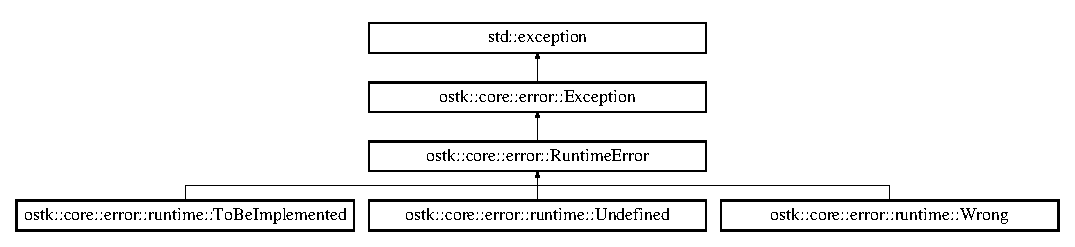
\includegraphics[height=2.871795cm]{classostk_1_1core_1_1error_1_1_runtime_error}
\end{center}
\end{figure}
\subsection*{Public Member Functions}
\begin{DoxyCompactItemize}
\item 
\hyperlink{classostk_1_1core_1_1error_1_1_runtime_error_ab86f511d582bd8904b8314ae71025498}{Runtime\+Error} (const \hyperlink{classostk_1_1core_1_1types_1_1_string}{String} \&a\+Message)
\item 
{\footnotesize template$<$typename ... Args$>$ }\\\hyperlink{classostk_1_1core_1_1error_1_1_runtime_error_a9affbbaa722f639547f9c4d1c9f0a421}{Runtime\+Error} (const char $\ast$a\+Format, Args... an\+Argument\+List)
\item 
\hyperlink{classostk_1_1core_1_1error_1_1_runtime_error_a65b0f31efc6a6825703553b8383e1668}{$\sim$\+Runtime\+Error} ()
\item 
virtual const char $\ast$ \hyperlink{classostk_1_1core_1_1error_1_1_runtime_error_a671d71ab5483eaa1ce5cc3400747ded1}{what} () const noexcept override
\end{DoxyCompactItemize}


\subsection{Detailed Description}
Runtime error class. 

\subsection{Constructor \& Destructor Documentation}
\mbox{\Hypertarget{classostk_1_1core_1_1error_1_1_runtime_error_ab86f511d582bd8904b8314ae71025498}\label{classostk_1_1core_1_1error_1_1_runtime_error_ab86f511d582bd8904b8314ae71025498}} 
\index{ostk\+::core\+::error\+::\+Runtime\+Error@{ostk\+::core\+::error\+::\+Runtime\+Error}!Runtime\+Error@{Runtime\+Error}}
\index{Runtime\+Error@{Runtime\+Error}!ostk\+::core\+::error\+::\+Runtime\+Error@{ostk\+::core\+::error\+::\+Runtime\+Error}}
\subsubsection{\texorpdfstring{Runtime\+Error()}{RuntimeError()}\hspace{0.1cm}{\footnotesize\ttfamily [1/2]}}
{\footnotesize\ttfamily ostk\+::core\+::error\+::\+Runtime\+Error\+::\+Runtime\+Error (\begin{DoxyParamCaption}\item[{const \hyperlink{classostk_1_1core_1_1types_1_1_string}{String} \&}]{a\+Message }\end{DoxyParamCaption})}

\mbox{\Hypertarget{classostk_1_1core_1_1error_1_1_runtime_error_a9affbbaa722f639547f9c4d1c9f0a421}\label{classostk_1_1core_1_1error_1_1_runtime_error_a9affbbaa722f639547f9c4d1c9f0a421}} 
\index{ostk\+::core\+::error\+::\+Runtime\+Error@{ostk\+::core\+::error\+::\+Runtime\+Error}!Runtime\+Error@{Runtime\+Error}}
\index{Runtime\+Error@{Runtime\+Error}!ostk\+::core\+::error\+::\+Runtime\+Error@{ostk\+::core\+::error\+::\+Runtime\+Error}}
\subsubsection{\texorpdfstring{Runtime\+Error()}{RuntimeError()}\hspace{0.1cm}{\footnotesize\ttfamily [2/2]}}
{\footnotesize\ttfamily template$<$typename ... Args$>$ \\
ostk\+::core\+::error\+::\+Runtime\+Error\+::\+Runtime\+Error (\begin{DoxyParamCaption}\item[{const char $\ast$}]{a\+Format,  }\item[{Args...}]{an\+Argument\+List }\end{DoxyParamCaption})\hspace{0.3cm}{\ttfamily [inline]}}

\mbox{\Hypertarget{classostk_1_1core_1_1error_1_1_runtime_error_a65b0f31efc6a6825703553b8383e1668}\label{classostk_1_1core_1_1error_1_1_runtime_error_a65b0f31efc6a6825703553b8383e1668}} 
\index{ostk\+::core\+::error\+::\+Runtime\+Error@{ostk\+::core\+::error\+::\+Runtime\+Error}!````~Runtime\+Error@{$\sim$\+Runtime\+Error}}
\index{````~Runtime\+Error@{$\sim$\+Runtime\+Error}!ostk\+::core\+::error\+::\+Runtime\+Error@{ostk\+::core\+::error\+::\+Runtime\+Error}}
\subsubsection{\texorpdfstring{$\sim$\+Runtime\+Error()}{~RuntimeError()}}
{\footnotesize\ttfamily ostk\+::core\+::error\+::\+Runtime\+Error\+::$\sim$\+Runtime\+Error (\begin{DoxyParamCaption}{ }\end{DoxyParamCaption})}



\subsection{Member Function Documentation}
\mbox{\Hypertarget{classostk_1_1core_1_1error_1_1_runtime_error_a671d71ab5483eaa1ce5cc3400747ded1}\label{classostk_1_1core_1_1error_1_1_runtime_error_a671d71ab5483eaa1ce5cc3400747ded1}} 
\index{ostk\+::core\+::error\+::\+Runtime\+Error@{ostk\+::core\+::error\+::\+Runtime\+Error}!what@{what}}
\index{what@{what}!ostk\+::core\+::error\+::\+Runtime\+Error@{ostk\+::core\+::error\+::\+Runtime\+Error}}
\subsubsection{\texorpdfstring{what()}{what()}}
{\footnotesize\ttfamily const char $\ast$ ostk\+::core\+::error\+::\+Runtime\+Error\+::what (\begin{DoxyParamCaption}{ }\end{DoxyParamCaption}) const\hspace{0.3cm}{\ttfamily [override]}, {\ttfamily [virtual]}, {\ttfamily [noexcept]}}



Reimplemented from \hyperlink{classostk_1_1core_1_1error_1_1_exception_ae34ebc20a97277da6e2472b6bb8e3812}{ostk\+::core\+::error\+::\+Exception}.



The documentation for this class was generated from the following files\+:\begin{DoxyCompactItemize}
\item 
include/\+Open\+Space\+Toolkit/\+Core/\+Error/\hyperlink{_runtime_error_8hpp}{Runtime\+Error.\+hpp}\item 
src/\+Open\+Space\+Toolkit/\+Core/\+Error/\hyperlink{_runtime_error_8cpp}{Runtime\+Error.\+cpp}\end{DoxyCompactItemize}

\hypertarget{classostk_1_1core_1_1logger_1_1_sink}{}\section{ostk\+:\+:core\+:\+:logger\+:\+:Sink Class Reference}
\label{classostk_1_1core_1_1logger_1_1_sink}\index{ostk\+::core\+::logger\+::\+Sink@{ostk\+::core\+::logger\+::\+Sink}}


Log sink.  




{\ttfamily \#include $<$Sink.\+hpp$>$}

\subsection*{Public Member Functions}
\begin{DoxyCompactItemize}
\item 
\hyperlink{classostk_1_1core_1_1logger_1_1_sink_ac28d087af4ba547441eec028b959ab91}{Sink} (const \hyperlink{classostk_1_1core_1_1logger_1_1sinks_1_1_sink}{sinks\+::\+Sink} \&a\+Sink)
\item 
\hyperlink{classostk_1_1core_1_1logger_1_1_sink_aadf37265845ad9648afcb7d07f0756ca}{Sink} (const \hyperlink{classostk_1_1core_1_1logger_1_1_sink}{Sink} \&a\+Sink)
\item 
void \hyperlink{classostk_1_1core_1_1logger_1_1_sink_aba09f6fd4b47c6dbcf755834ea531c17}{enable} ()
\item 
void \hyperlink{classostk_1_1core_1_1logger_1_1_sink_a0ab42f184deb76938ae3ab97f690fbaf}{disable} ()
\item 
void \hyperlink{classostk_1_1core_1_1logger_1_1_sink_a7dba5710eb033df07cfe7ead0104a122}{add\+Channel} (const \hyperlink{classostk_1_1core_1_1types_1_1_string}{String} \&a\+Channel)
\item 
void \hyperlink{classostk_1_1core_1_1logger_1_1_sink_ac11d2e63d7643cdbf8a24718ce2dd216}{remove\+Channel} (const \hyperlink{classostk_1_1core_1_1types_1_1_string}{String} \&a\+Channel)
\end{DoxyCompactItemize}
\subsection*{Static Public Member Functions}
\begin{DoxyCompactItemize}
\item 
static \hyperlink{classostk_1_1core_1_1logger_1_1_sink}{Sink} \hyperlink{classostk_1_1core_1_1logger_1_1_sink_a363d47c4b76945b5aa75f0b21b7740c2}{Console} (const \hyperlink{namespaceostk_1_1core_1_1logger_a52d02954e094391f067befffe7f3cae9}{Severity} \&a\+Severity)
\end{DoxyCompactItemize}


\subsection{Detailed Description}
Log sink. 

\subsection{Constructor \& Destructor Documentation}
\mbox{\Hypertarget{classostk_1_1core_1_1logger_1_1_sink_ac28d087af4ba547441eec028b959ab91}\label{classostk_1_1core_1_1logger_1_1_sink_ac28d087af4ba547441eec028b959ab91}} 
\index{ostk\+::core\+::logger\+::\+Sink@{ostk\+::core\+::logger\+::\+Sink}!Sink@{Sink}}
\index{Sink@{Sink}!ostk\+::core\+::logger\+::\+Sink@{ostk\+::core\+::logger\+::\+Sink}}
\subsubsection{\texorpdfstring{Sink()}{Sink()}\hspace{0.1cm}{\footnotesize\ttfamily [1/2]}}
{\footnotesize\ttfamily ostk\+::core\+::logger\+::\+Sink\+::\+Sink (\begin{DoxyParamCaption}\item[{const \hyperlink{classostk_1_1core_1_1logger_1_1sinks_1_1_sink}{sinks\+::\+Sink} \&}]{a\+Sink }\end{DoxyParamCaption})}

\mbox{\Hypertarget{classostk_1_1core_1_1logger_1_1_sink_aadf37265845ad9648afcb7d07f0756ca}\label{classostk_1_1core_1_1logger_1_1_sink_aadf37265845ad9648afcb7d07f0756ca}} 
\index{ostk\+::core\+::logger\+::\+Sink@{ostk\+::core\+::logger\+::\+Sink}!Sink@{Sink}}
\index{Sink@{Sink}!ostk\+::core\+::logger\+::\+Sink@{ostk\+::core\+::logger\+::\+Sink}}
\subsubsection{\texorpdfstring{Sink()}{Sink()}\hspace{0.1cm}{\footnotesize\ttfamily [2/2]}}
{\footnotesize\ttfamily ostk\+::core\+::logger\+::\+Sink\+::\+Sink (\begin{DoxyParamCaption}\item[{const \hyperlink{classostk_1_1core_1_1logger_1_1_sink}{Sink} \&}]{a\+Sink }\end{DoxyParamCaption})}



\subsection{Member Function Documentation}
\mbox{\Hypertarget{classostk_1_1core_1_1logger_1_1_sink_a7dba5710eb033df07cfe7ead0104a122}\label{classostk_1_1core_1_1logger_1_1_sink_a7dba5710eb033df07cfe7ead0104a122}} 
\index{ostk\+::core\+::logger\+::\+Sink@{ostk\+::core\+::logger\+::\+Sink}!add\+Channel@{add\+Channel}}
\index{add\+Channel@{add\+Channel}!ostk\+::core\+::logger\+::\+Sink@{ostk\+::core\+::logger\+::\+Sink}}
\subsubsection{\texorpdfstring{add\+Channel()}{addChannel()}}
{\footnotesize\ttfamily void ostk\+::core\+::logger\+::\+Sink\+::add\+Channel (\begin{DoxyParamCaption}\item[{const \hyperlink{classostk_1_1core_1_1types_1_1_string}{String} \&}]{a\+Channel }\end{DoxyParamCaption})}

\mbox{\Hypertarget{classostk_1_1core_1_1logger_1_1_sink_a363d47c4b76945b5aa75f0b21b7740c2}\label{classostk_1_1core_1_1logger_1_1_sink_a363d47c4b76945b5aa75f0b21b7740c2}} 
\index{ostk\+::core\+::logger\+::\+Sink@{ostk\+::core\+::logger\+::\+Sink}!Console@{Console}}
\index{Console@{Console}!ostk\+::core\+::logger\+::\+Sink@{ostk\+::core\+::logger\+::\+Sink}}
\subsubsection{\texorpdfstring{Console()}{Console()}}
{\footnotesize\ttfamily static \hyperlink{classostk_1_1core_1_1logger_1_1_sink}{Sink} ostk\+::core\+::logger\+::\+Sink\+::\+Console (\begin{DoxyParamCaption}\item[{const \hyperlink{namespaceostk_1_1core_1_1logger_a52d02954e094391f067befffe7f3cae9}{Severity} \&}]{a\+Severity }\end{DoxyParamCaption})\hspace{0.3cm}{\ttfamily [static]}}

\mbox{\Hypertarget{classostk_1_1core_1_1logger_1_1_sink_a0ab42f184deb76938ae3ab97f690fbaf}\label{classostk_1_1core_1_1logger_1_1_sink_a0ab42f184deb76938ae3ab97f690fbaf}} 
\index{ostk\+::core\+::logger\+::\+Sink@{ostk\+::core\+::logger\+::\+Sink}!disable@{disable}}
\index{disable@{disable}!ostk\+::core\+::logger\+::\+Sink@{ostk\+::core\+::logger\+::\+Sink}}
\subsubsection{\texorpdfstring{disable()}{disable()}}
{\footnotesize\ttfamily void ostk\+::core\+::logger\+::\+Sink\+::disable (\begin{DoxyParamCaption}{ }\end{DoxyParamCaption})}

\mbox{\Hypertarget{classostk_1_1core_1_1logger_1_1_sink_aba09f6fd4b47c6dbcf755834ea531c17}\label{classostk_1_1core_1_1logger_1_1_sink_aba09f6fd4b47c6dbcf755834ea531c17}} 
\index{ostk\+::core\+::logger\+::\+Sink@{ostk\+::core\+::logger\+::\+Sink}!enable@{enable}}
\index{enable@{enable}!ostk\+::core\+::logger\+::\+Sink@{ostk\+::core\+::logger\+::\+Sink}}
\subsubsection{\texorpdfstring{enable()}{enable()}}
{\footnotesize\ttfamily void ostk\+::core\+::logger\+::\+Sink\+::enable (\begin{DoxyParamCaption}{ }\end{DoxyParamCaption})}

\mbox{\Hypertarget{classostk_1_1core_1_1logger_1_1_sink_ac11d2e63d7643cdbf8a24718ce2dd216}\label{classostk_1_1core_1_1logger_1_1_sink_ac11d2e63d7643cdbf8a24718ce2dd216}} 
\index{ostk\+::core\+::logger\+::\+Sink@{ostk\+::core\+::logger\+::\+Sink}!remove\+Channel@{remove\+Channel}}
\index{remove\+Channel@{remove\+Channel}!ostk\+::core\+::logger\+::\+Sink@{ostk\+::core\+::logger\+::\+Sink}}
\subsubsection{\texorpdfstring{remove\+Channel()}{removeChannel()}}
{\footnotesize\ttfamily void ostk\+::core\+::logger\+::\+Sink\+::remove\+Channel (\begin{DoxyParamCaption}\item[{const \hyperlink{classostk_1_1core_1_1types_1_1_string}{String} \&}]{a\+Channel }\end{DoxyParamCaption})}



The documentation for this class was generated from the following file\+:\begin{DoxyCompactItemize}
\item 
include/\+Open\+Space\+Toolkit/\+Core/\+Logger/\hyperlink{_sink_8hpp}{Sink.\+hpp}\end{DoxyCompactItemize}

\hypertarget{classostk_1_1core_1_1logger_1_1sinks_1_1_sink}{}\section{ostk\+:\+:core\+:\+:logger\+:\+:sinks\+:\+:Sink Class Reference}
\label{classostk_1_1core_1_1logger_1_1sinks_1_1_sink}\index{ostk\+::core\+::logger\+::sinks\+::\+Sink@{ostk\+::core\+::logger\+::sinks\+::\+Sink}}


Log sink base.  




{\ttfamily \#include $<$Sink.\+hpp$>$}

Inheritance diagram for ostk\+:\+:core\+:\+:logger\+:\+:sinks\+:\+:Sink\+:\begin{figure}[H]
\begin{center}
\leavevmode
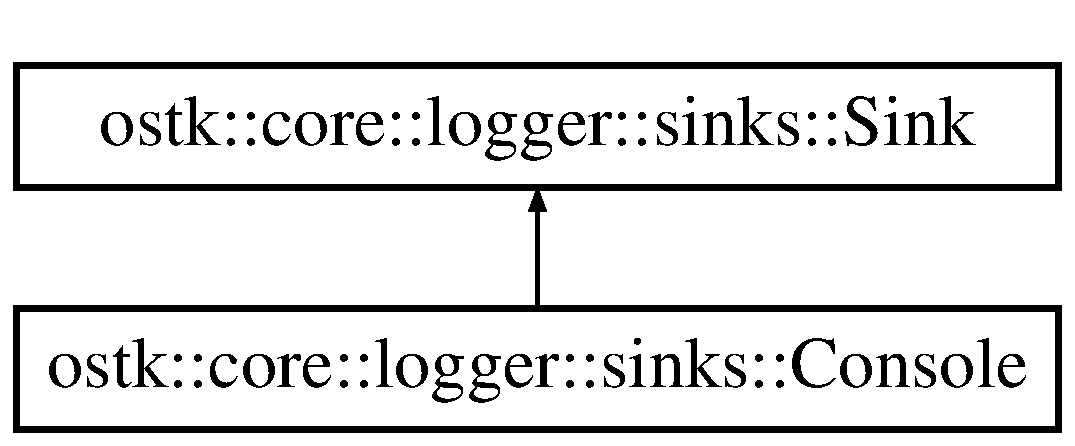
\includegraphics[height=2.000000cm]{classostk_1_1core_1_1logger_1_1sinks_1_1_sink}
\end{center}
\end{figure}
\subsection*{Public Member Functions}
\begin{DoxyCompactItemize}
\item 
\hyperlink{classostk_1_1core_1_1logger_1_1sinks_1_1_sink_ada8f8e327dbc3776096d5d6fc9a0f0d5}{Sink} (const \hyperlink{namespaceostk_1_1core_1_1logger_a52d02954e094391f067befffe7f3cae9}{Severity} \&a\+Severity)
\item 
virtual \hyperlink{classostk_1_1core_1_1logger_1_1sinks_1_1_sink_a9b7fa855f7463981958c4c6c55bd9096}{$\sim$\+Sink} ()=0
\item 
virtual \hyperlink{classostk_1_1core_1_1logger_1_1sinks_1_1_sink}{Sink} $\ast$ \hyperlink{classostk_1_1core_1_1logger_1_1sinks_1_1_sink_a0e6b41f9b4626b5229370f71bd27be32}{clone} () const =0
\item 
bool \hyperlink{classostk_1_1core_1_1logger_1_1sinks_1_1_sink_ab0f84d1b7492172f86ce6b6965d1ec06}{is\+Enabled} () const
\item 
bool \hyperlink{classostk_1_1core_1_1logger_1_1sinks_1_1_sink_acc00e2ba3b9bc7643cf6219fae51dccc}{is\+Line\+Id\+Logged} () const
\item 
bool \hyperlink{classostk_1_1core_1_1logger_1_1sinks_1_1_sink_a3589e31f6b53bbec59d224cedafe5e31}{is\+Severity\+Logged} () const
\item 
bool \hyperlink{classostk_1_1core_1_1logger_1_1sinks_1_1_sink_ad811def520afbde684ed5c370923bbde}{is\+Timestamp\+Logged} () const
\item 
bool \hyperlink{classostk_1_1core_1_1logger_1_1sinks_1_1_sink_a635805c31e3a9b39c0c812ae8c122722}{is\+Thread\+Logged} () const
\item 
bool \hyperlink{classostk_1_1core_1_1logger_1_1sinks_1_1_sink_aea22f037f19aa1b8582aa7c4d508c409}{is\+Scope\+Logged} () const
\item 
bool \hyperlink{classostk_1_1core_1_1logger_1_1sinks_1_1_sink_af747351b5769b05e566000503ace7c6b}{is\+File\+Logged} () const
\item 
bool \hyperlink{classostk_1_1core_1_1logger_1_1sinks_1_1_sink_a70376798333269bf550f3f2b010f30fd}{is\+Line\+Logged} () const
\item 
bool \hyperlink{classostk_1_1core_1_1logger_1_1sinks_1_1_sink_ada08c6affa847f0276a27b6f394b6b4f}{is\+Function\+Logged} () const
\item 
bool \hyperlink{classostk_1_1core_1_1logger_1_1sinks_1_1_sink_aab319e29565fc6d5cf800a6155e8bc75}{is\+Channel\+Logged} () const
\item 
virtual void \hyperlink{classostk_1_1core_1_1logger_1_1sinks_1_1_sink_a355c81571a4a34bb162c1dc5fe631c89}{enable} ()=0
\item 
virtual void \hyperlink{classostk_1_1core_1_1logger_1_1sinks_1_1_sink_a3e347ffee80e3c2ee50ff0edf9265115}{disable} ()=0
\item 
void \hyperlink{classostk_1_1core_1_1logger_1_1sinks_1_1_sink_a4f8fe98afdb070da6afde4c775e238ac}{add\+Channel} (const \hyperlink{classostk_1_1core_1_1types_1_1_string}{String} \&a\+Channel)
\item 
void \hyperlink{classostk_1_1core_1_1logger_1_1sinks_1_1_sink_a0cfd70c07a03a157b0810cc2a2c1f030}{remove\+Channel} (const \hyperlink{classostk_1_1core_1_1types_1_1_string}{String} \&a\+Channel)
\end{DoxyCompactItemize}
\subsection*{Protected Attributes}
\begin{DoxyCompactItemize}
\item 
bool \hyperlink{classostk_1_1core_1_1logger_1_1sinks_1_1_sink_a36b5e1e2ef67889e3787920d792ee061}{enabled\+\_\+}
\item 
\hyperlink{namespaceostk_1_1core_1_1logger_a52d02954e094391f067befffe7f3cae9}{Severity} \hyperlink{classostk_1_1core_1_1logger_1_1sinks_1_1_sink_ab204e1f685dc9a208adbe06d5e0f6354}{severity\+\_\+}
\item 
bool \hyperlink{classostk_1_1core_1_1logger_1_1sinks_1_1_sink_a303e83d8ad7459122bae68e585163bf5}{line\+Id\+Enabled\+\_\+}
\item 
bool \hyperlink{classostk_1_1core_1_1logger_1_1sinks_1_1_sink_ae99e33f0e5f7d8df226464095f11cb5c}{severity\+Enabled\+\_\+}
\item 
bool \hyperlink{classostk_1_1core_1_1logger_1_1sinks_1_1_sink_ac18e9ae38b09bd049e900c6e7a5b5386}{timestamp\+Enabled\+\_\+}
\item 
bool \hyperlink{classostk_1_1core_1_1logger_1_1sinks_1_1_sink_a9c0c43f72f9bbc8276a64c6040696ff0}{thread\+Enabled\+\_\+}
\item 
bool \hyperlink{classostk_1_1core_1_1logger_1_1sinks_1_1_sink_ac4dc4261e28962fe1cdb41588d204099}{scope\+Enabled\+\_\+}
\item 
bool \hyperlink{classostk_1_1core_1_1logger_1_1sinks_1_1_sink_aba0425e9f715065b3e70da2a77b0819f}{file\+Enabled\+\_\+}
\item 
bool \hyperlink{classostk_1_1core_1_1logger_1_1sinks_1_1_sink_a7bd015ab0a98cd25eb8ada72ee342122}{line\+Enabled\+\_\+}
\item 
bool \hyperlink{classostk_1_1core_1_1logger_1_1sinks_1_1_sink_a59b6b95a6803713533da26d0b5c9f771}{function\+Enabled\+\_\+}
\item 
bool \hyperlink{classostk_1_1core_1_1logger_1_1sinks_1_1_sink_a7ce30490e1d1b9969ca9442483a26644}{channel\+Enabled\+\_\+}
\item 
\hyperlink{classostk_1_1core_1_1ctnr_1_1_array}{Array}$<$ \hyperlink{classostk_1_1core_1_1types_1_1_string}{String} $>$ \hyperlink{classostk_1_1core_1_1logger_1_1sinks_1_1_sink_a63c6b779d1dc982331aa9b388ab10313}{channels\+\_\+}
\end{DoxyCompactItemize}


\subsection{Detailed Description}
Log sink base. 

\subsection{Constructor \& Destructor Documentation}
\mbox{\Hypertarget{classostk_1_1core_1_1logger_1_1sinks_1_1_sink_ada8f8e327dbc3776096d5d6fc9a0f0d5}\label{classostk_1_1core_1_1logger_1_1sinks_1_1_sink_ada8f8e327dbc3776096d5d6fc9a0f0d5}} 
\index{ostk\+::core\+::logger\+::sinks\+::\+Sink@{ostk\+::core\+::logger\+::sinks\+::\+Sink}!Sink@{Sink}}
\index{Sink@{Sink}!ostk\+::core\+::logger\+::sinks\+::\+Sink@{ostk\+::core\+::logger\+::sinks\+::\+Sink}}
\subsubsection{\texorpdfstring{Sink()}{Sink()}}
{\footnotesize\ttfamily ostk\+::core\+::logger\+::sinks\+::\+Sink\+::\+Sink (\begin{DoxyParamCaption}\item[{const \hyperlink{namespaceostk_1_1core_1_1logger_a52d02954e094391f067befffe7f3cae9}{Severity} \&}]{a\+Severity }\end{DoxyParamCaption})}

\mbox{\Hypertarget{classostk_1_1core_1_1logger_1_1sinks_1_1_sink_a9b7fa855f7463981958c4c6c55bd9096}\label{classostk_1_1core_1_1logger_1_1sinks_1_1_sink_a9b7fa855f7463981958c4c6c55bd9096}} 
\index{ostk\+::core\+::logger\+::sinks\+::\+Sink@{ostk\+::core\+::logger\+::sinks\+::\+Sink}!````~Sink@{$\sim$\+Sink}}
\index{````~Sink@{$\sim$\+Sink}!ostk\+::core\+::logger\+::sinks\+::\+Sink@{ostk\+::core\+::logger\+::sinks\+::\+Sink}}
\subsubsection{\texorpdfstring{$\sim$\+Sink()}{~Sink()}}
{\footnotesize\ttfamily virtual ostk\+::core\+::logger\+::sinks\+::\+Sink\+::$\sim$\+Sink (\begin{DoxyParamCaption}{ }\end{DoxyParamCaption})\hspace{0.3cm}{\ttfamily [pure virtual]}}



\subsection{Member Function Documentation}
\mbox{\Hypertarget{classostk_1_1core_1_1logger_1_1sinks_1_1_sink_a4f8fe98afdb070da6afde4c775e238ac}\label{classostk_1_1core_1_1logger_1_1sinks_1_1_sink_a4f8fe98afdb070da6afde4c775e238ac}} 
\index{ostk\+::core\+::logger\+::sinks\+::\+Sink@{ostk\+::core\+::logger\+::sinks\+::\+Sink}!add\+Channel@{add\+Channel}}
\index{add\+Channel@{add\+Channel}!ostk\+::core\+::logger\+::sinks\+::\+Sink@{ostk\+::core\+::logger\+::sinks\+::\+Sink}}
\subsubsection{\texorpdfstring{add\+Channel()}{addChannel()}}
{\footnotesize\ttfamily void ostk\+::core\+::logger\+::sinks\+::\+Sink\+::add\+Channel (\begin{DoxyParamCaption}\item[{const \hyperlink{classostk_1_1core_1_1types_1_1_string}{String} \&}]{a\+Channel }\end{DoxyParamCaption})}

\mbox{\Hypertarget{classostk_1_1core_1_1logger_1_1sinks_1_1_sink_a0e6b41f9b4626b5229370f71bd27be32}\label{classostk_1_1core_1_1logger_1_1sinks_1_1_sink_a0e6b41f9b4626b5229370f71bd27be32}} 
\index{ostk\+::core\+::logger\+::sinks\+::\+Sink@{ostk\+::core\+::logger\+::sinks\+::\+Sink}!clone@{clone}}
\index{clone@{clone}!ostk\+::core\+::logger\+::sinks\+::\+Sink@{ostk\+::core\+::logger\+::sinks\+::\+Sink}}
\subsubsection{\texorpdfstring{clone()}{clone()}}
{\footnotesize\ttfamily virtual \hyperlink{classostk_1_1core_1_1logger_1_1sinks_1_1_sink}{Sink}$\ast$ ostk\+::core\+::logger\+::sinks\+::\+Sink\+::clone (\begin{DoxyParamCaption}{ }\end{DoxyParamCaption}) const\hspace{0.3cm}{\ttfamily [pure virtual]}}



Implemented in \hyperlink{classostk_1_1core_1_1logger_1_1sinks_1_1_console_ab906fb3918a362c527489091e006d521}{ostk\+::core\+::logger\+::sinks\+::\+Console}.

\mbox{\Hypertarget{classostk_1_1core_1_1logger_1_1sinks_1_1_sink_a3e347ffee80e3c2ee50ff0edf9265115}\label{classostk_1_1core_1_1logger_1_1sinks_1_1_sink_a3e347ffee80e3c2ee50ff0edf9265115}} 
\index{ostk\+::core\+::logger\+::sinks\+::\+Sink@{ostk\+::core\+::logger\+::sinks\+::\+Sink}!disable@{disable}}
\index{disable@{disable}!ostk\+::core\+::logger\+::sinks\+::\+Sink@{ostk\+::core\+::logger\+::sinks\+::\+Sink}}
\subsubsection{\texorpdfstring{disable()}{disable()}}
{\footnotesize\ttfamily virtual void ostk\+::core\+::logger\+::sinks\+::\+Sink\+::disable (\begin{DoxyParamCaption}{ }\end{DoxyParamCaption})\hspace{0.3cm}{\ttfamily [pure virtual]}}



Implemented in \hyperlink{classostk_1_1core_1_1logger_1_1sinks_1_1_console_a5872f5826955ff7f6371bce6ea320253}{ostk\+::core\+::logger\+::sinks\+::\+Console}.

\mbox{\Hypertarget{classostk_1_1core_1_1logger_1_1sinks_1_1_sink_a355c81571a4a34bb162c1dc5fe631c89}\label{classostk_1_1core_1_1logger_1_1sinks_1_1_sink_a355c81571a4a34bb162c1dc5fe631c89}} 
\index{ostk\+::core\+::logger\+::sinks\+::\+Sink@{ostk\+::core\+::logger\+::sinks\+::\+Sink}!enable@{enable}}
\index{enable@{enable}!ostk\+::core\+::logger\+::sinks\+::\+Sink@{ostk\+::core\+::logger\+::sinks\+::\+Sink}}
\subsubsection{\texorpdfstring{enable()}{enable()}}
{\footnotesize\ttfamily virtual void ostk\+::core\+::logger\+::sinks\+::\+Sink\+::enable (\begin{DoxyParamCaption}{ }\end{DoxyParamCaption})\hspace{0.3cm}{\ttfamily [pure virtual]}}



Implemented in \hyperlink{classostk_1_1core_1_1logger_1_1sinks_1_1_console_a684825bbab717a14f9c83712c054d1d9}{ostk\+::core\+::logger\+::sinks\+::\+Console}.

\mbox{\Hypertarget{classostk_1_1core_1_1logger_1_1sinks_1_1_sink_aab319e29565fc6d5cf800a6155e8bc75}\label{classostk_1_1core_1_1logger_1_1sinks_1_1_sink_aab319e29565fc6d5cf800a6155e8bc75}} 
\index{ostk\+::core\+::logger\+::sinks\+::\+Sink@{ostk\+::core\+::logger\+::sinks\+::\+Sink}!is\+Channel\+Logged@{is\+Channel\+Logged}}
\index{is\+Channel\+Logged@{is\+Channel\+Logged}!ostk\+::core\+::logger\+::sinks\+::\+Sink@{ostk\+::core\+::logger\+::sinks\+::\+Sink}}
\subsubsection{\texorpdfstring{is\+Channel\+Logged()}{isChannelLogged()}}
{\footnotesize\ttfamily bool ostk\+::core\+::logger\+::sinks\+::\+Sink\+::is\+Channel\+Logged (\begin{DoxyParamCaption}{ }\end{DoxyParamCaption}) const}

\mbox{\Hypertarget{classostk_1_1core_1_1logger_1_1sinks_1_1_sink_ab0f84d1b7492172f86ce6b6965d1ec06}\label{classostk_1_1core_1_1logger_1_1sinks_1_1_sink_ab0f84d1b7492172f86ce6b6965d1ec06}} 
\index{ostk\+::core\+::logger\+::sinks\+::\+Sink@{ostk\+::core\+::logger\+::sinks\+::\+Sink}!is\+Enabled@{is\+Enabled}}
\index{is\+Enabled@{is\+Enabled}!ostk\+::core\+::logger\+::sinks\+::\+Sink@{ostk\+::core\+::logger\+::sinks\+::\+Sink}}
\subsubsection{\texorpdfstring{is\+Enabled()}{isEnabled()}}
{\footnotesize\ttfamily bool ostk\+::core\+::logger\+::sinks\+::\+Sink\+::is\+Enabled (\begin{DoxyParamCaption}{ }\end{DoxyParamCaption}) const}

\mbox{\Hypertarget{classostk_1_1core_1_1logger_1_1sinks_1_1_sink_af747351b5769b05e566000503ace7c6b}\label{classostk_1_1core_1_1logger_1_1sinks_1_1_sink_af747351b5769b05e566000503ace7c6b}} 
\index{ostk\+::core\+::logger\+::sinks\+::\+Sink@{ostk\+::core\+::logger\+::sinks\+::\+Sink}!is\+File\+Logged@{is\+File\+Logged}}
\index{is\+File\+Logged@{is\+File\+Logged}!ostk\+::core\+::logger\+::sinks\+::\+Sink@{ostk\+::core\+::logger\+::sinks\+::\+Sink}}
\subsubsection{\texorpdfstring{is\+File\+Logged()}{isFileLogged()}}
{\footnotesize\ttfamily bool ostk\+::core\+::logger\+::sinks\+::\+Sink\+::is\+File\+Logged (\begin{DoxyParamCaption}{ }\end{DoxyParamCaption}) const}

\mbox{\Hypertarget{classostk_1_1core_1_1logger_1_1sinks_1_1_sink_ada08c6affa847f0276a27b6f394b6b4f}\label{classostk_1_1core_1_1logger_1_1sinks_1_1_sink_ada08c6affa847f0276a27b6f394b6b4f}} 
\index{ostk\+::core\+::logger\+::sinks\+::\+Sink@{ostk\+::core\+::logger\+::sinks\+::\+Sink}!is\+Function\+Logged@{is\+Function\+Logged}}
\index{is\+Function\+Logged@{is\+Function\+Logged}!ostk\+::core\+::logger\+::sinks\+::\+Sink@{ostk\+::core\+::logger\+::sinks\+::\+Sink}}
\subsubsection{\texorpdfstring{is\+Function\+Logged()}{isFunctionLogged()}}
{\footnotesize\ttfamily bool ostk\+::core\+::logger\+::sinks\+::\+Sink\+::is\+Function\+Logged (\begin{DoxyParamCaption}{ }\end{DoxyParamCaption}) const}

\mbox{\Hypertarget{classostk_1_1core_1_1logger_1_1sinks_1_1_sink_acc00e2ba3b9bc7643cf6219fae51dccc}\label{classostk_1_1core_1_1logger_1_1sinks_1_1_sink_acc00e2ba3b9bc7643cf6219fae51dccc}} 
\index{ostk\+::core\+::logger\+::sinks\+::\+Sink@{ostk\+::core\+::logger\+::sinks\+::\+Sink}!is\+Line\+Id\+Logged@{is\+Line\+Id\+Logged}}
\index{is\+Line\+Id\+Logged@{is\+Line\+Id\+Logged}!ostk\+::core\+::logger\+::sinks\+::\+Sink@{ostk\+::core\+::logger\+::sinks\+::\+Sink}}
\subsubsection{\texorpdfstring{is\+Line\+Id\+Logged()}{isLineIdLogged()}}
{\footnotesize\ttfamily bool ostk\+::core\+::logger\+::sinks\+::\+Sink\+::is\+Line\+Id\+Logged (\begin{DoxyParamCaption}{ }\end{DoxyParamCaption}) const}

\mbox{\Hypertarget{classostk_1_1core_1_1logger_1_1sinks_1_1_sink_a70376798333269bf550f3f2b010f30fd}\label{classostk_1_1core_1_1logger_1_1sinks_1_1_sink_a70376798333269bf550f3f2b010f30fd}} 
\index{ostk\+::core\+::logger\+::sinks\+::\+Sink@{ostk\+::core\+::logger\+::sinks\+::\+Sink}!is\+Line\+Logged@{is\+Line\+Logged}}
\index{is\+Line\+Logged@{is\+Line\+Logged}!ostk\+::core\+::logger\+::sinks\+::\+Sink@{ostk\+::core\+::logger\+::sinks\+::\+Sink}}
\subsubsection{\texorpdfstring{is\+Line\+Logged()}{isLineLogged()}}
{\footnotesize\ttfamily bool ostk\+::core\+::logger\+::sinks\+::\+Sink\+::is\+Line\+Logged (\begin{DoxyParamCaption}{ }\end{DoxyParamCaption}) const}

\mbox{\Hypertarget{classostk_1_1core_1_1logger_1_1sinks_1_1_sink_aea22f037f19aa1b8582aa7c4d508c409}\label{classostk_1_1core_1_1logger_1_1sinks_1_1_sink_aea22f037f19aa1b8582aa7c4d508c409}} 
\index{ostk\+::core\+::logger\+::sinks\+::\+Sink@{ostk\+::core\+::logger\+::sinks\+::\+Sink}!is\+Scope\+Logged@{is\+Scope\+Logged}}
\index{is\+Scope\+Logged@{is\+Scope\+Logged}!ostk\+::core\+::logger\+::sinks\+::\+Sink@{ostk\+::core\+::logger\+::sinks\+::\+Sink}}
\subsubsection{\texorpdfstring{is\+Scope\+Logged()}{isScopeLogged()}}
{\footnotesize\ttfamily bool ostk\+::core\+::logger\+::sinks\+::\+Sink\+::is\+Scope\+Logged (\begin{DoxyParamCaption}{ }\end{DoxyParamCaption}) const}

\mbox{\Hypertarget{classostk_1_1core_1_1logger_1_1sinks_1_1_sink_a3589e31f6b53bbec59d224cedafe5e31}\label{classostk_1_1core_1_1logger_1_1sinks_1_1_sink_a3589e31f6b53bbec59d224cedafe5e31}} 
\index{ostk\+::core\+::logger\+::sinks\+::\+Sink@{ostk\+::core\+::logger\+::sinks\+::\+Sink}!is\+Severity\+Logged@{is\+Severity\+Logged}}
\index{is\+Severity\+Logged@{is\+Severity\+Logged}!ostk\+::core\+::logger\+::sinks\+::\+Sink@{ostk\+::core\+::logger\+::sinks\+::\+Sink}}
\subsubsection{\texorpdfstring{is\+Severity\+Logged()}{isSeverityLogged()}}
{\footnotesize\ttfamily bool ostk\+::core\+::logger\+::sinks\+::\+Sink\+::is\+Severity\+Logged (\begin{DoxyParamCaption}{ }\end{DoxyParamCaption}) const}

\mbox{\Hypertarget{classostk_1_1core_1_1logger_1_1sinks_1_1_sink_a635805c31e3a9b39c0c812ae8c122722}\label{classostk_1_1core_1_1logger_1_1sinks_1_1_sink_a635805c31e3a9b39c0c812ae8c122722}} 
\index{ostk\+::core\+::logger\+::sinks\+::\+Sink@{ostk\+::core\+::logger\+::sinks\+::\+Sink}!is\+Thread\+Logged@{is\+Thread\+Logged}}
\index{is\+Thread\+Logged@{is\+Thread\+Logged}!ostk\+::core\+::logger\+::sinks\+::\+Sink@{ostk\+::core\+::logger\+::sinks\+::\+Sink}}
\subsubsection{\texorpdfstring{is\+Thread\+Logged()}{isThreadLogged()}}
{\footnotesize\ttfamily bool ostk\+::core\+::logger\+::sinks\+::\+Sink\+::is\+Thread\+Logged (\begin{DoxyParamCaption}{ }\end{DoxyParamCaption}) const}

\mbox{\Hypertarget{classostk_1_1core_1_1logger_1_1sinks_1_1_sink_ad811def520afbde684ed5c370923bbde}\label{classostk_1_1core_1_1logger_1_1sinks_1_1_sink_ad811def520afbde684ed5c370923bbde}} 
\index{ostk\+::core\+::logger\+::sinks\+::\+Sink@{ostk\+::core\+::logger\+::sinks\+::\+Sink}!is\+Timestamp\+Logged@{is\+Timestamp\+Logged}}
\index{is\+Timestamp\+Logged@{is\+Timestamp\+Logged}!ostk\+::core\+::logger\+::sinks\+::\+Sink@{ostk\+::core\+::logger\+::sinks\+::\+Sink}}
\subsubsection{\texorpdfstring{is\+Timestamp\+Logged()}{isTimestampLogged()}}
{\footnotesize\ttfamily bool ostk\+::core\+::logger\+::sinks\+::\+Sink\+::is\+Timestamp\+Logged (\begin{DoxyParamCaption}{ }\end{DoxyParamCaption}) const}

\mbox{\Hypertarget{classostk_1_1core_1_1logger_1_1sinks_1_1_sink_a0cfd70c07a03a157b0810cc2a2c1f030}\label{classostk_1_1core_1_1logger_1_1sinks_1_1_sink_a0cfd70c07a03a157b0810cc2a2c1f030}} 
\index{ostk\+::core\+::logger\+::sinks\+::\+Sink@{ostk\+::core\+::logger\+::sinks\+::\+Sink}!remove\+Channel@{remove\+Channel}}
\index{remove\+Channel@{remove\+Channel}!ostk\+::core\+::logger\+::sinks\+::\+Sink@{ostk\+::core\+::logger\+::sinks\+::\+Sink}}
\subsubsection{\texorpdfstring{remove\+Channel()}{removeChannel()}}
{\footnotesize\ttfamily void ostk\+::core\+::logger\+::sinks\+::\+Sink\+::remove\+Channel (\begin{DoxyParamCaption}\item[{const \hyperlink{classostk_1_1core_1_1types_1_1_string}{String} \&}]{a\+Channel }\end{DoxyParamCaption})}



\subsection{Member Data Documentation}
\mbox{\Hypertarget{classostk_1_1core_1_1logger_1_1sinks_1_1_sink_a7ce30490e1d1b9969ca9442483a26644}\label{classostk_1_1core_1_1logger_1_1sinks_1_1_sink_a7ce30490e1d1b9969ca9442483a26644}} 
\index{ostk\+::core\+::logger\+::sinks\+::\+Sink@{ostk\+::core\+::logger\+::sinks\+::\+Sink}!channel\+Enabled\+\_\+@{channel\+Enabled\+\_\+}}
\index{channel\+Enabled\+\_\+@{channel\+Enabled\+\_\+}!ostk\+::core\+::logger\+::sinks\+::\+Sink@{ostk\+::core\+::logger\+::sinks\+::\+Sink}}
\subsubsection{\texorpdfstring{channel\+Enabled\+\_\+}{channelEnabled\_}}
{\footnotesize\ttfamily bool ostk\+::core\+::logger\+::sinks\+::\+Sink\+::channel\+Enabled\+\_\+\hspace{0.3cm}{\ttfamily [protected]}}

\mbox{\Hypertarget{classostk_1_1core_1_1logger_1_1sinks_1_1_sink_a63c6b779d1dc982331aa9b388ab10313}\label{classostk_1_1core_1_1logger_1_1sinks_1_1_sink_a63c6b779d1dc982331aa9b388ab10313}} 
\index{ostk\+::core\+::logger\+::sinks\+::\+Sink@{ostk\+::core\+::logger\+::sinks\+::\+Sink}!channels\+\_\+@{channels\+\_\+}}
\index{channels\+\_\+@{channels\+\_\+}!ostk\+::core\+::logger\+::sinks\+::\+Sink@{ostk\+::core\+::logger\+::sinks\+::\+Sink}}
\subsubsection{\texorpdfstring{channels\+\_\+}{channels\_}}
{\footnotesize\ttfamily \hyperlink{classostk_1_1core_1_1ctnr_1_1_array}{Array}$<$\hyperlink{classostk_1_1core_1_1types_1_1_string}{String}$>$ ostk\+::core\+::logger\+::sinks\+::\+Sink\+::channels\+\_\+\hspace{0.3cm}{\ttfamily [protected]}}

\mbox{\Hypertarget{classostk_1_1core_1_1logger_1_1sinks_1_1_sink_a36b5e1e2ef67889e3787920d792ee061}\label{classostk_1_1core_1_1logger_1_1sinks_1_1_sink_a36b5e1e2ef67889e3787920d792ee061}} 
\index{ostk\+::core\+::logger\+::sinks\+::\+Sink@{ostk\+::core\+::logger\+::sinks\+::\+Sink}!enabled\+\_\+@{enabled\+\_\+}}
\index{enabled\+\_\+@{enabled\+\_\+}!ostk\+::core\+::logger\+::sinks\+::\+Sink@{ostk\+::core\+::logger\+::sinks\+::\+Sink}}
\subsubsection{\texorpdfstring{enabled\+\_\+}{enabled\_}}
{\footnotesize\ttfamily bool ostk\+::core\+::logger\+::sinks\+::\+Sink\+::enabled\+\_\+\hspace{0.3cm}{\ttfamily [protected]}}

\mbox{\Hypertarget{classostk_1_1core_1_1logger_1_1sinks_1_1_sink_aba0425e9f715065b3e70da2a77b0819f}\label{classostk_1_1core_1_1logger_1_1sinks_1_1_sink_aba0425e9f715065b3e70da2a77b0819f}} 
\index{ostk\+::core\+::logger\+::sinks\+::\+Sink@{ostk\+::core\+::logger\+::sinks\+::\+Sink}!file\+Enabled\+\_\+@{file\+Enabled\+\_\+}}
\index{file\+Enabled\+\_\+@{file\+Enabled\+\_\+}!ostk\+::core\+::logger\+::sinks\+::\+Sink@{ostk\+::core\+::logger\+::sinks\+::\+Sink}}
\subsubsection{\texorpdfstring{file\+Enabled\+\_\+}{fileEnabled\_}}
{\footnotesize\ttfamily bool ostk\+::core\+::logger\+::sinks\+::\+Sink\+::file\+Enabled\+\_\+\hspace{0.3cm}{\ttfamily [protected]}}

\mbox{\Hypertarget{classostk_1_1core_1_1logger_1_1sinks_1_1_sink_a59b6b95a6803713533da26d0b5c9f771}\label{classostk_1_1core_1_1logger_1_1sinks_1_1_sink_a59b6b95a6803713533da26d0b5c9f771}} 
\index{ostk\+::core\+::logger\+::sinks\+::\+Sink@{ostk\+::core\+::logger\+::sinks\+::\+Sink}!function\+Enabled\+\_\+@{function\+Enabled\+\_\+}}
\index{function\+Enabled\+\_\+@{function\+Enabled\+\_\+}!ostk\+::core\+::logger\+::sinks\+::\+Sink@{ostk\+::core\+::logger\+::sinks\+::\+Sink}}
\subsubsection{\texorpdfstring{function\+Enabled\+\_\+}{functionEnabled\_}}
{\footnotesize\ttfamily bool ostk\+::core\+::logger\+::sinks\+::\+Sink\+::function\+Enabled\+\_\+\hspace{0.3cm}{\ttfamily [protected]}}

\mbox{\Hypertarget{classostk_1_1core_1_1logger_1_1sinks_1_1_sink_a7bd015ab0a98cd25eb8ada72ee342122}\label{classostk_1_1core_1_1logger_1_1sinks_1_1_sink_a7bd015ab0a98cd25eb8ada72ee342122}} 
\index{ostk\+::core\+::logger\+::sinks\+::\+Sink@{ostk\+::core\+::logger\+::sinks\+::\+Sink}!line\+Enabled\+\_\+@{line\+Enabled\+\_\+}}
\index{line\+Enabled\+\_\+@{line\+Enabled\+\_\+}!ostk\+::core\+::logger\+::sinks\+::\+Sink@{ostk\+::core\+::logger\+::sinks\+::\+Sink}}
\subsubsection{\texorpdfstring{line\+Enabled\+\_\+}{lineEnabled\_}}
{\footnotesize\ttfamily bool ostk\+::core\+::logger\+::sinks\+::\+Sink\+::line\+Enabled\+\_\+\hspace{0.3cm}{\ttfamily [protected]}}

\mbox{\Hypertarget{classostk_1_1core_1_1logger_1_1sinks_1_1_sink_a303e83d8ad7459122bae68e585163bf5}\label{classostk_1_1core_1_1logger_1_1sinks_1_1_sink_a303e83d8ad7459122bae68e585163bf5}} 
\index{ostk\+::core\+::logger\+::sinks\+::\+Sink@{ostk\+::core\+::logger\+::sinks\+::\+Sink}!line\+Id\+Enabled\+\_\+@{line\+Id\+Enabled\+\_\+}}
\index{line\+Id\+Enabled\+\_\+@{line\+Id\+Enabled\+\_\+}!ostk\+::core\+::logger\+::sinks\+::\+Sink@{ostk\+::core\+::logger\+::sinks\+::\+Sink}}
\subsubsection{\texorpdfstring{line\+Id\+Enabled\+\_\+}{lineIdEnabled\_}}
{\footnotesize\ttfamily bool ostk\+::core\+::logger\+::sinks\+::\+Sink\+::line\+Id\+Enabled\+\_\+\hspace{0.3cm}{\ttfamily [protected]}}

\mbox{\Hypertarget{classostk_1_1core_1_1logger_1_1sinks_1_1_sink_ac4dc4261e28962fe1cdb41588d204099}\label{classostk_1_1core_1_1logger_1_1sinks_1_1_sink_ac4dc4261e28962fe1cdb41588d204099}} 
\index{ostk\+::core\+::logger\+::sinks\+::\+Sink@{ostk\+::core\+::logger\+::sinks\+::\+Sink}!scope\+Enabled\+\_\+@{scope\+Enabled\+\_\+}}
\index{scope\+Enabled\+\_\+@{scope\+Enabled\+\_\+}!ostk\+::core\+::logger\+::sinks\+::\+Sink@{ostk\+::core\+::logger\+::sinks\+::\+Sink}}
\subsubsection{\texorpdfstring{scope\+Enabled\+\_\+}{scopeEnabled\_}}
{\footnotesize\ttfamily bool ostk\+::core\+::logger\+::sinks\+::\+Sink\+::scope\+Enabled\+\_\+\hspace{0.3cm}{\ttfamily [protected]}}

\mbox{\Hypertarget{classostk_1_1core_1_1logger_1_1sinks_1_1_sink_ab204e1f685dc9a208adbe06d5e0f6354}\label{classostk_1_1core_1_1logger_1_1sinks_1_1_sink_ab204e1f685dc9a208adbe06d5e0f6354}} 
\index{ostk\+::core\+::logger\+::sinks\+::\+Sink@{ostk\+::core\+::logger\+::sinks\+::\+Sink}!severity\+\_\+@{severity\+\_\+}}
\index{severity\+\_\+@{severity\+\_\+}!ostk\+::core\+::logger\+::sinks\+::\+Sink@{ostk\+::core\+::logger\+::sinks\+::\+Sink}}
\subsubsection{\texorpdfstring{severity\+\_\+}{severity\_}}
{\footnotesize\ttfamily \hyperlink{namespaceostk_1_1core_1_1logger_a52d02954e094391f067befffe7f3cae9}{Severity} ostk\+::core\+::logger\+::sinks\+::\+Sink\+::severity\+\_\+\hspace{0.3cm}{\ttfamily [protected]}}

\mbox{\Hypertarget{classostk_1_1core_1_1logger_1_1sinks_1_1_sink_ae99e33f0e5f7d8df226464095f11cb5c}\label{classostk_1_1core_1_1logger_1_1sinks_1_1_sink_ae99e33f0e5f7d8df226464095f11cb5c}} 
\index{ostk\+::core\+::logger\+::sinks\+::\+Sink@{ostk\+::core\+::logger\+::sinks\+::\+Sink}!severity\+Enabled\+\_\+@{severity\+Enabled\+\_\+}}
\index{severity\+Enabled\+\_\+@{severity\+Enabled\+\_\+}!ostk\+::core\+::logger\+::sinks\+::\+Sink@{ostk\+::core\+::logger\+::sinks\+::\+Sink}}
\subsubsection{\texorpdfstring{severity\+Enabled\+\_\+}{severityEnabled\_}}
{\footnotesize\ttfamily bool ostk\+::core\+::logger\+::sinks\+::\+Sink\+::severity\+Enabled\+\_\+\hspace{0.3cm}{\ttfamily [protected]}}

\mbox{\Hypertarget{classostk_1_1core_1_1logger_1_1sinks_1_1_sink_a9c0c43f72f9bbc8276a64c6040696ff0}\label{classostk_1_1core_1_1logger_1_1sinks_1_1_sink_a9c0c43f72f9bbc8276a64c6040696ff0}} 
\index{ostk\+::core\+::logger\+::sinks\+::\+Sink@{ostk\+::core\+::logger\+::sinks\+::\+Sink}!thread\+Enabled\+\_\+@{thread\+Enabled\+\_\+}}
\index{thread\+Enabled\+\_\+@{thread\+Enabled\+\_\+}!ostk\+::core\+::logger\+::sinks\+::\+Sink@{ostk\+::core\+::logger\+::sinks\+::\+Sink}}
\subsubsection{\texorpdfstring{thread\+Enabled\+\_\+}{threadEnabled\_}}
{\footnotesize\ttfamily bool ostk\+::core\+::logger\+::sinks\+::\+Sink\+::thread\+Enabled\+\_\+\hspace{0.3cm}{\ttfamily [protected]}}

\mbox{\Hypertarget{classostk_1_1core_1_1logger_1_1sinks_1_1_sink_ac18e9ae38b09bd049e900c6e7a5b5386}\label{classostk_1_1core_1_1logger_1_1sinks_1_1_sink_ac18e9ae38b09bd049e900c6e7a5b5386}} 
\index{ostk\+::core\+::logger\+::sinks\+::\+Sink@{ostk\+::core\+::logger\+::sinks\+::\+Sink}!timestamp\+Enabled\+\_\+@{timestamp\+Enabled\+\_\+}}
\index{timestamp\+Enabled\+\_\+@{timestamp\+Enabled\+\_\+}!ostk\+::core\+::logger\+::sinks\+::\+Sink@{ostk\+::core\+::logger\+::sinks\+::\+Sink}}
\subsubsection{\texorpdfstring{timestamp\+Enabled\+\_\+}{timestampEnabled\_}}
{\footnotesize\ttfamily bool ostk\+::core\+::logger\+::sinks\+::\+Sink\+::timestamp\+Enabled\+\_\+\hspace{0.3cm}{\ttfamily [protected]}}



The documentation for this class was generated from the following file\+:\begin{DoxyCompactItemize}
\item 
include/\+Open\+Space\+Toolkit/\+Core/\+Logger/\+Sinks/\hyperlink{_sinks_2_sink_8hpp}{Sink.\+hpp}\end{DoxyCompactItemize}

\hypertarget{classostk_1_1core_1_1logger_1_1_source}{}\section{ostk\+:\+:core\+:\+:logger\+:\+:Source Class Reference}
\label{classostk_1_1core_1_1logger_1_1_source}\index{ostk\+::core\+::logger\+::\+Source@{ostk\+::core\+::logger\+::\+Source}}


Log source.  




{\ttfamily \#include $<$Source.\+hpp$>$}

\subsection*{Public Member Functions}
\begin{DoxyCompactItemize}
\item 
\hyperlink{classostk_1_1core_1_1logger_1_1_source_a02ece6e1d79d574bcf5e1917dd5cc728}{Source} (const \hyperlink{classostk_1_1core_1_1types_1_1_string}{String} \&a\+Channel)
\item 
\hyperlink{classostk_1_1core_1_1logger_1_1_source_a8e1107712c9b1ab9e5506230d32c7a06}{Source} (const \hyperlink{classostk_1_1core_1_1logger_1_1_source}{Source} \&a\+Source)
\item 
\hyperlink{classostk_1_1core_1_1logger_1_1_source}{Source} \& \hyperlink{classostk_1_1core_1_1logger_1_1_source_ae6e4fbcb686bcd0b03808f31d9b30bbf}{operator=} (const \hyperlink{classostk_1_1core_1_1logger_1_1_source}{Source} \&a\+Source)
\item 
bool \hyperlink{classostk_1_1core_1_1logger_1_1_source_ad990358e832e3deb4b5d0cae908d10b7}{is\+Defined} () const
\end{DoxyCompactItemize}
\subsection*{Static Public Member Functions}
\begin{DoxyCompactItemize}
\item 
static \hyperlink{classostk_1_1core_1_1logger_1_1_source}{Source} \hyperlink{classostk_1_1core_1_1logger_1_1_source_a272a407ccc75d370b259efc685d48063}{Undefined} ()
\end{DoxyCompactItemize}
\subsection*{Public Attributes}
\begin{DoxyCompactItemize}
\item 
Unique$<$ \hyperlink{classostk_1_1core_1_1logger_1_1sources_1_1_source}{sources\+::\+Source} $>$ \hyperlink{classostk_1_1core_1_1logger_1_1_source_abbe1b964fe5f7a462fb8ab67f2007662}{source\+U\+Ptr\+\_\+}
\end{DoxyCompactItemize}


\subsection{Detailed Description}
Log source. 

\subsection{Constructor \& Destructor Documentation}
\mbox{\Hypertarget{classostk_1_1core_1_1logger_1_1_source_a02ece6e1d79d574bcf5e1917dd5cc728}\label{classostk_1_1core_1_1logger_1_1_source_a02ece6e1d79d574bcf5e1917dd5cc728}} 
\index{ostk\+::core\+::logger\+::\+Source@{ostk\+::core\+::logger\+::\+Source}!Source@{Source}}
\index{Source@{Source}!ostk\+::core\+::logger\+::\+Source@{ostk\+::core\+::logger\+::\+Source}}
\subsubsection{\texorpdfstring{Source()}{Source()}\hspace{0.1cm}{\footnotesize\ttfamily [1/2]}}
{\footnotesize\ttfamily ostk\+::core\+::logger\+::\+Source\+::\+Source (\begin{DoxyParamCaption}\item[{const \hyperlink{classostk_1_1core_1_1types_1_1_string}{String} \&}]{a\+Channel }\end{DoxyParamCaption})}

\mbox{\Hypertarget{classostk_1_1core_1_1logger_1_1_source_a8e1107712c9b1ab9e5506230d32c7a06}\label{classostk_1_1core_1_1logger_1_1_source_a8e1107712c9b1ab9e5506230d32c7a06}} 
\index{ostk\+::core\+::logger\+::\+Source@{ostk\+::core\+::logger\+::\+Source}!Source@{Source}}
\index{Source@{Source}!ostk\+::core\+::logger\+::\+Source@{ostk\+::core\+::logger\+::\+Source}}
\subsubsection{\texorpdfstring{Source()}{Source()}\hspace{0.1cm}{\footnotesize\ttfamily [2/2]}}
{\footnotesize\ttfamily ostk\+::core\+::logger\+::\+Source\+::\+Source (\begin{DoxyParamCaption}\item[{const \hyperlink{classostk_1_1core_1_1logger_1_1_source}{Source} \&}]{a\+Source }\end{DoxyParamCaption})}



\subsection{Member Function Documentation}
\mbox{\Hypertarget{classostk_1_1core_1_1logger_1_1_source_ad990358e832e3deb4b5d0cae908d10b7}\label{classostk_1_1core_1_1logger_1_1_source_ad990358e832e3deb4b5d0cae908d10b7}} 
\index{ostk\+::core\+::logger\+::\+Source@{ostk\+::core\+::logger\+::\+Source}!is\+Defined@{is\+Defined}}
\index{is\+Defined@{is\+Defined}!ostk\+::core\+::logger\+::\+Source@{ostk\+::core\+::logger\+::\+Source}}
\subsubsection{\texorpdfstring{is\+Defined()}{isDefined()}}
{\footnotesize\ttfamily bool ostk\+::core\+::logger\+::\+Source\+::is\+Defined (\begin{DoxyParamCaption}{ }\end{DoxyParamCaption}) const}

\mbox{\Hypertarget{classostk_1_1core_1_1logger_1_1_source_ae6e4fbcb686bcd0b03808f31d9b30bbf}\label{classostk_1_1core_1_1logger_1_1_source_ae6e4fbcb686bcd0b03808f31d9b30bbf}} 
\index{ostk\+::core\+::logger\+::\+Source@{ostk\+::core\+::logger\+::\+Source}!operator=@{operator=}}
\index{operator=@{operator=}!ostk\+::core\+::logger\+::\+Source@{ostk\+::core\+::logger\+::\+Source}}
\subsubsection{\texorpdfstring{operator=()}{operator=()}}
{\footnotesize\ttfamily \hyperlink{classostk_1_1core_1_1logger_1_1_source}{Source}\& ostk\+::core\+::logger\+::\+Source\+::operator= (\begin{DoxyParamCaption}\item[{const \hyperlink{classostk_1_1core_1_1logger_1_1_source}{Source} \&}]{a\+Source }\end{DoxyParamCaption})}

\mbox{\Hypertarget{classostk_1_1core_1_1logger_1_1_source_a272a407ccc75d370b259efc685d48063}\label{classostk_1_1core_1_1logger_1_1_source_a272a407ccc75d370b259efc685d48063}} 
\index{ostk\+::core\+::logger\+::\+Source@{ostk\+::core\+::logger\+::\+Source}!Undefined@{Undefined}}
\index{Undefined@{Undefined}!ostk\+::core\+::logger\+::\+Source@{ostk\+::core\+::logger\+::\+Source}}
\subsubsection{\texorpdfstring{Undefined()}{Undefined()}}
{\footnotesize\ttfamily static \hyperlink{classostk_1_1core_1_1logger_1_1_source}{Source} ostk\+::core\+::logger\+::\+Source\+::\+Undefined (\begin{DoxyParamCaption}{ }\end{DoxyParamCaption})\hspace{0.3cm}{\ttfamily [static]}}



\subsection{Member Data Documentation}
\mbox{\Hypertarget{classostk_1_1core_1_1logger_1_1_source_abbe1b964fe5f7a462fb8ab67f2007662}\label{classostk_1_1core_1_1logger_1_1_source_abbe1b964fe5f7a462fb8ab67f2007662}} 
\index{ostk\+::core\+::logger\+::\+Source@{ostk\+::core\+::logger\+::\+Source}!source\+U\+Ptr\+\_\+@{source\+U\+Ptr\+\_\+}}
\index{source\+U\+Ptr\+\_\+@{source\+U\+Ptr\+\_\+}!ostk\+::core\+::logger\+::\+Source@{ostk\+::core\+::logger\+::\+Source}}
\subsubsection{\texorpdfstring{source\+U\+Ptr\+\_\+}{sourceUPtr\_}}
{\footnotesize\ttfamily Unique$<$\hyperlink{classostk_1_1core_1_1logger_1_1sources_1_1_source}{sources\+::\+Source}$>$ ostk\+::core\+::logger\+::\+Source\+::source\+U\+Ptr\+\_\+}



The documentation for this class was generated from the following file\+:\begin{DoxyCompactItemize}
\item 
include/\+Open\+Space\+Toolkit/\+Core/\+Logger/\hyperlink{_source_8hpp}{Source.\+hpp}\end{DoxyCompactItemize}

\hypertarget{classostk_1_1core_1_1logger_1_1sources_1_1_source}{}\section{ostk\+:\+:core\+:\+:logger\+:\+:sources\+:\+:Source Class Reference}
\label{classostk_1_1core_1_1logger_1_1sources_1_1_source}\index{ostk\+::core\+::logger\+::sources\+::\+Source@{ostk\+::core\+::logger\+::sources\+::\+Source}}


Log source base.  




{\ttfamily \#include $<$Source.\+hpp$>$}

\subsection*{Public Member Functions}
\begin{DoxyCompactItemize}
\item 
\hyperlink{classostk_1_1core_1_1logger_1_1sources_1_1_source_a41da7a2ae5373f66cce639177b3cc463}{Source} (const \hyperlink{classostk_1_1core_1_1types_1_1_string}{String} \&a\+Channel)
\item 
\hyperlink{classostk_1_1core_1_1logger_1_1sources_1_1_source_a5cc73c7801acb5d8c3e411ece21118cb}{Source} (const \hyperlink{classostk_1_1core_1_1logger_1_1sources_1_1_source}{Source} \&a\+Source)
\item 
\hyperlink{classostk_1_1core_1_1logger_1_1sources_1_1_source_a7b5d8956adcc78e593806111fc4e81f4}{$\sim$\+Source} ()
\item 
virtual \hyperlink{classostk_1_1core_1_1logger_1_1sources_1_1_source}{Source} $\ast$ \hyperlink{classostk_1_1core_1_1logger_1_1sources_1_1_source_acab589eb280846091323d9b7d3157fc4}{clone} () const
\item 
\hyperlink{classostk_1_1core_1_1logger_1_1sources_1_1_source}{Source} \& \hyperlink{classostk_1_1core_1_1logger_1_1sources_1_1_source_a17c7f7ee66390536117fc77c997172be}{operator=} (const \hyperlink{classostk_1_1core_1_1logger_1_1sources_1_1_source}{Source} \&a\+Source)=default
\item 
void $\ast$ \hyperlink{classostk_1_1core_1_1logger_1_1sources_1_1_source_a2101c2fe9538ed093808309eba594513}{access\+Logger} ()
\end{DoxyCompactItemize}
\subsection*{Friends}
\begin{DoxyCompactItemize}
\item 
class \hyperlink{classostk_1_1core_1_1logger_1_1sources_1_1_source_a64fbdb62a5c5f27e0d022da36aab93d9}{Pump}
\end{DoxyCompactItemize}


\subsection{Detailed Description}
Log source base. 

\subsection{Constructor \& Destructor Documentation}
\mbox{\Hypertarget{classostk_1_1core_1_1logger_1_1sources_1_1_source_a41da7a2ae5373f66cce639177b3cc463}\label{classostk_1_1core_1_1logger_1_1sources_1_1_source_a41da7a2ae5373f66cce639177b3cc463}} 
\index{ostk\+::core\+::logger\+::sources\+::\+Source@{ostk\+::core\+::logger\+::sources\+::\+Source}!Source@{Source}}
\index{Source@{Source}!ostk\+::core\+::logger\+::sources\+::\+Source@{ostk\+::core\+::logger\+::sources\+::\+Source}}
\subsubsection{\texorpdfstring{Source()}{Source()}\hspace{0.1cm}{\footnotesize\ttfamily [1/2]}}
{\footnotesize\ttfamily ostk\+::core\+::logger\+::sources\+::\+Source\+::\+Source (\begin{DoxyParamCaption}\item[{const \hyperlink{classostk_1_1core_1_1types_1_1_string}{String} \&}]{a\+Channel }\end{DoxyParamCaption})}

\mbox{\Hypertarget{classostk_1_1core_1_1logger_1_1sources_1_1_source_a5cc73c7801acb5d8c3e411ece21118cb}\label{classostk_1_1core_1_1logger_1_1sources_1_1_source_a5cc73c7801acb5d8c3e411ece21118cb}} 
\index{ostk\+::core\+::logger\+::sources\+::\+Source@{ostk\+::core\+::logger\+::sources\+::\+Source}!Source@{Source}}
\index{Source@{Source}!ostk\+::core\+::logger\+::sources\+::\+Source@{ostk\+::core\+::logger\+::sources\+::\+Source}}
\subsubsection{\texorpdfstring{Source()}{Source()}\hspace{0.1cm}{\footnotesize\ttfamily [2/2]}}
{\footnotesize\ttfamily ostk\+::core\+::logger\+::sources\+::\+Source\+::\+Source (\begin{DoxyParamCaption}\item[{const \hyperlink{classostk_1_1core_1_1logger_1_1sources_1_1_source}{Source} \&}]{a\+Source }\end{DoxyParamCaption})}

\mbox{\Hypertarget{classostk_1_1core_1_1logger_1_1sources_1_1_source_a7b5d8956adcc78e593806111fc4e81f4}\label{classostk_1_1core_1_1logger_1_1sources_1_1_source_a7b5d8956adcc78e593806111fc4e81f4}} 
\index{ostk\+::core\+::logger\+::sources\+::\+Source@{ostk\+::core\+::logger\+::sources\+::\+Source}!````~Source@{$\sim$\+Source}}
\index{````~Source@{$\sim$\+Source}!ostk\+::core\+::logger\+::sources\+::\+Source@{ostk\+::core\+::logger\+::sources\+::\+Source}}
\subsubsection{\texorpdfstring{$\sim$\+Source()}{~Source()}}
{\footnotesize\ttfamily ostk\+::core\+::logger\+::sources\+::\+Source\+::$\sim$\+Source (\begin{DoxyParamCaption}{ }\end{DoxyParamCaption})}



\subsection{Member Function Documentation}
\mbox{\Hypertarget{classostk_1_1core_1_1logger_1_1sources_1_1_source_a2101c2fe9538ed093808309eba594513}\label{classostk_1_1core_1_1logger_1_1sources_1_1_source_a2101c2fe9538ed093808309eba594513}} 
\index{ostk\+::core\+::logger\+::sources\+::\+Source@{ostk\+::core\+::logger\+::sources\+::\+Source}!access\+Logger@{access\+Logger}}
\index{access\+Logger@{access\+Logger}!ostk\+::core\+::logger\+::sources\+::\+Source@{ostk\+::core\+::logger\+::sources\+::\+Source}}
\subsubsection{\texorpdfstring{access\+Logger()}{accessLogger()}}
{\footnotesize\ttfamily void$\ast$ ostk\+::core\+::logger\+::sources\+::\+Source\+::access\+Logger (\begin{DoxyParamCaption}{ }\end{DoxyParamCaption})}

\mbox{\Hypertarget{classostk_1_1core_1_1logger_1_1sources_1_1_source_acab589eb280846091323d9b7d3157fc4}\label{classostk_1_1core_1_1logger_1_1sources_1_1_source_acab589eb280846091323d9b7d3157fc4}} 
\index{ostk\+::core\+::logger\+::sources\+::\+Source@{ostk\+::core\+::logger\+::sources\+::\+Source}!clone@{clone}}
\index{clone@{clone}!ostk\+::core\+::logger\+::sources\+::\+Source@{ostk\+::core\+::logger\+::sources\+::\+Source}}
\subsubsection{\texorpdfstring{clone()}{clone()}}
{\footnotesize\ttfamily virtual \hyperlink{classostk_1_1core_1_1logger_1_1sources_1_1_source}{Source}$\ast$ ostk\+::core\+::logger\+::sources\+::\+Source\+::clone (\begin{DoxyParamCaption}{ }\end{DoxyParamCaption}) const\hspace{0.3cm}{\ttfamily [virtual]}}

\mbox{\Hypertarget{classostk_1_1core_1_1logger_1_1sources_1_1_source_a17c7f7ee66390536117fc77c997172be}\label{classostk_1_1core_1_1logger_1_1sources_1_1_source_a17c7f7ee66390536117fc77c997172be}} 
\index{ostk\+::core\+::logger\+::sources\+::\+Source@{ostk\+::core\+::logger\+::sources\+::\+Source}!operator=@{operator=}}
\index{operator=@{operator=}!ostk\+::core\+::logger\+::sources\+::\+Source@{ostk\+::core\+::logger\+::sources\+::\+Source}}
\subsubsection{\texorpdfstring{operator=()}{operator=()}}
{\footnotesize\ttfamily \hyperlink{classostk_1_1core_1_1logger_1_1sources_1_1_source}{Source}\& ostk\+::core\+::logger\+::sources\+::\+Source\+::operator= (\begin{DoxyParamCaption}\item[{const \hyperlink{classostk_1_1core_1_1logger_1_1sources_1_1_source}{Source} \&}]{a\+Source }\end{DoxyParamCaption})\hspace{0.3cm}{\ttfamily [default]}}



\subsection{Friends And Related Function Documentation}
\mbox{\Hypertarget{classostk_1_1core_1_1logger_1_1sources_1_1_source_a64fbdb62a5c5f27e0d022da36aab93d9}\label{classostk_1_1core_1_1logger_1_1sources_1_1_source_a64fbdb62a5c5f27e0d022da36aab93d9}} 
\index{ostk\+::core\+::logger\+::sources\+::\+Source@{ostk\+::core\+::logger\+::sources\+::\+Source}!Pump@{Pump}}
\index{Pump@{Pump}!ostk\+::core\+::logger\+::sources\+::\+Source@{ostk\+::core\+::logger\+::sources\+::\+Source}}
\subsubsection{\texorpdfstring{Pump}{Pump}}
{\footnotesize\ttfamily friend class \hyperlink{classostk_1_1core_1_1logger_1_1_pump}{Pump}\hspace{0.3cm}{\ttfamily [friend]}}



The documentation for this class was generated from the following file\+:\begin{DoxyCompactItemize}
\item 
include/\+Open\+Space\+Toolkit/\+Core/\+Logger/\+Sources/\hyperlink{_sources_2_source_8hpp}{Source.\+hpp}\end{DoxyCompactItemize}

\hypertarget{classostk_1_1core_1_1ctnr_1_1_stack}{}\section{ostk\+:\+:core\+:\+:ctnr\+:\+:Stack Class Reference}
\label{classostk_1_1core_1_1ctnr_1_1_stack}\index{ostk\+::core\+::ctnr\+::\+Stack@{ostk\+::core\+::ctnr\+::\+Stack}}


First-\/in, last-\/out (F\+I\+LO) container.  




{\ttfamily \#include $<$Stack.\+hpp$>$}

\subsection*{Public Member Functions}
\begin{DoxyCompactItemize}
\item 
\hyperlink{classostk_1_1core_1_1ctnr_1_1_stack_a0e02851144c2afaf2202846f90f950dc}{Stack} ()=delete
\item 
\hyperlink{classostk_1_1core_1_1ctnr_1_1_stack_add08ce0c3b6aaff44811abbe708bde78}{Stack} (const \hyperlink{classostk_1_1core_1_1ctnr_1_1_stack}{Stack} \&a\+Stack)
\item 
\hyperlink{classostk_1_1core_1_1ctnr_1_1_stack_afab136f4d7fbeeda04d89acc3be0b2b1}{$\sim$\+Stack} ()
\item 
\hyperlink{classostk_1_1core_1_1ctnr_1_1_stack}{Stack} \& \hyperlink{classostk_1_1core_1_1ctnr_1_1_stack_af5f86fc835c6e3d724a2f4c9d474b2a7}{operator=} (const \hyperlink{classostk_1_1core_1_1ctnr_1_1_stack}{Stack} \&a\+Stack) const
\item 
bool \hyperlink{classostk_1_1core_1_1ctnr_1_1_stack_a146e0c3f6914afa9e23106c395f895d2}{is\+Defined} () const
\end{DoxyCompactItemize}
\subsection*{Static Public Member Functions}
\begin{DoxyCompactItemize}
\item 
static \hyperlink{classostk_1_1core_1_1ctnr_1_1_stack}{Stack} \hyperlink{classostk_1_1core_1_1ctnr_1_1_stack_a720ccdf651af0a9d0b5659dea501d355}{Empty} ()
\item 
static \hyperlink{classostk_1_1core_1_1ctnr_1_1_stack}{Stack} \hyperlink{classostk_1_1core_1_1ctnr_1_1_stack_ac9a70eb14c3f8c1d6eb46ac5ea003714}{Object} (const \hyperlink{classostk_1_1core_1_1ctnr_1_1_object}{Object} \&an\+Object)
\end{DoxyCompactItemize}
\subsection*{Friends}
\begin{DoxyCompactItemize}
\item 
std\+::ostream \& \hyperlink{classostk_1_1core_1_1ctnr_1_1_stack_a042acac24eba66c740c7d3d48dfc0e46}{operator$<$$<$} (std\+::ostream \&an\+Output\+Stream, const \hyperlink{classostk_1_1core_1_1ctnr_1_1_stack}{Stack} \&a\+Stack)
\end{DoxyCompactItemize}


\subsection{Detailed Description}
First-\/in, last-\/out (F\+I\+LO) container. 

\subsection{Constructor \& Destructor Documentation}
\mbox{\Hypertarget{classostk_1_1core_1_1ctnr_1_1_stack_a0e02851144c2afaf2202846f90f950dc}\label{classostk_1_1core_1_1ctnr_1_1_stack_a0e02851144c2afaf2202846f90f950dc}} 
\index{ostk\+::core\+::ctnr\+::\+Stack@{ostk\+::core\+::ctnr\+::\+Stack}!Stack@{Stack}}
\index{Stack@{Stack}!ostk\+::core\+::ctnr\+::\+Stack@{ostk\+::core\+::ctnr\+::\+Stack}}
\subsubsection{\texorpdfstring{Stack()}{Stack()}\hspace{0.1cm}{\footnotesize\ttfamily [1/2]}}
{\footnotesize\ttfamily ostk\+::core\+::ctnr\+::\+Stack\+::\+Stack (\begin{DoxyParamCaption}{ }\end{DoxyParamCaption})\hspace{0.3cm}{\ttfamily [delete]}}

\mbox{\Hypertarget{classostk_1_1core_1_1ctnr_1_1_stack_add08ce0c3b6aaff44811abbe708bde78}\label{classostk_1_1core_1_1ctnr_1_1_stack_add08ce0c3b6aaff44811abbe708bde78}} 
\index{ostk\+::core\+::ctnr\+::\+Stack@{ostk\+::core\+::ctnr\+::\+Stack}!Stack@{Stack}}
\index{Stack@{Stack}!ostk\+::core\+::ctnr\+::\+Stack@{ostk\+::core\+::ctnr\+::\+Stack}}
\subsubsection{\texorpdfstring{Stack()}{Stack()}\hspace{0.1cm}{\footnotesize\ttfamily [2/2]}}
{\footnotesize\ttfamily ostk\+::core\+::ctnr\+::\+Stack\+::\+Stack (\begin{DoxyParamCaption}\item[{const \hyperlink{classostk_1_1core_1_1ctnr_1_1_stack}{Stack} \&}]{a\+Stack }\end{DoxyParamCaption})}

\mbox{\Hypertarget{classostk_1_1core_1_1ctnr_1_1_stack_afab136f4d7fbeeda04d89acc3be0b2b1}\label{classostk_1_1core_1_1ctnr_1_1_stack_afab136f4d7fbeeda04d89acc3be0b2b1}} 
\index{ostk\+::core\+::ctnr\+::\+Stack@{ostk\+::core\+::ctnr\+::\+Stack}!````~Stack@{$\sim$\+Stack}}
\index{````~Stack@{$\sim$\+Stack}!ostk\+::core\+::ctnr\+::\+Stack@{ostk\+::core\+::ctnr\+::\+Stack}}
\subsubsection{\texorpdfstring{$\sim$\+Stack()}{~Stack()}}
{\footnotesize\ttfamily ostk\+::core\+::ctnr\+::\+Stack\+::$\sim$\+Stack (\begin{DoxyParamCaption}{ }\end{DoxyParamCaption})}



\subsection{Member Function Documentation}
\mbox{\Hypertarget{classostk_1_1core_1_1ctnr_1_1_stack_a720ccdf651af0a9d0b5659dea501d355}\label{classostk_1_1core_1_1ctnr_1_1_stack_a720ccdf651af0a9d0b5659dea501d355}} 
\index{ostk\+::core\+::ctnr\+::\+Stack@{ostk\+::core\+::ctnr\+::\+Stack}!Empty@{Empty}}
\index{Empty@{Empty}!ostk\+::core\+::ctnr\+::\+Stack@{ostk\+::core\+::ctnr\+::\+Stack}}
\subsubsection{\texorpdfstring{Empty()}{Empty()}}
{\footnotesize\ttfamily static \hyperlink{classostk_1_1core_1_1ctnr_1_1_stack}{Stack} ostk\+::core\+::ctnr\+::\+Stack\+::\+Empty (\begin{DoxyParamCaption}{ }\end{DoxyParamCaption})\hspace{0.3cm}{\ttfamily [static]}}

\mbox{\Hypertarget{classostk_1_1core_1_1ctnr_1_1_stack_a146e0c3f6914afa9e23106c395f895d2}\label{classostk_1_1core_1_1ctnr_1_1_stack_a146e0c3f6914afa9e23106c395f895d2}} 
\index{ostk\+::core\+::ctnr\+::\+Stack@{ostk\+::core\+::ctnr\+::\+Stack}!is\+Defined@{is\+Defined}}
\index{is\+Defined@{is\+Defined}!ostk\+::core\+::ctnr\+::\+Stack@{ostk\+::core\+::ctnr\+::\+Stack}}
\subsubsection{\texorpdfstring{is\+Defined()}{isDefined()}}
{\footnotesize\ttfamily bool ostk\+::core\+::ctnr\+::\+Stack\+::is\+Defined (\begin{DoxyParamCaption}{ }\end{DoxyParamCaption}) const}

\mbox{\Hypertarget{classostk_1_1core_1_1ctnr_1_1_stack_ac9a70eb14c3f8c1d6eb46ac5ea003714}\label{classostk_1_1core_1_1ctnr_1_1_stack_ac9a70eb14c3f8c1d6eb46ac5ea003714}} 
\index{ostk\+::core\+::ctnr\+::\+Stack@{ostk\+::core\+::ctnr\+::\+Stack}!Object@{Object}}
\index{Object@{Object}!ostk\+::core\+::ctnr\+::\+Stack@{ostk\+::core\+::ctnr\+::\+Stack}}
\subsubsection{\texorpdfstring{Object()}{Object()}}
{\footnotesize\ttfamily static \hyperlink{classostk_1_1core_1_1ctnr_1_1_stack}{Stack} ostk\+::core\+::ctnr\+::\+Stack\+::\+Object (\begin{DoxyParamCaption}\item[{const \hyperlink{classostk_1_1core_1_1ctnr_1_1_object}{Object} \&}]{an\+Object }\end{DoxyParamCaption})\hspace{0.3cm}{\ttfamily [static]}}

\mbox{\Hypertarget{classostk_1_1core_1_1ctnr_1_1_stack_af5f86fc835c6e3d724a2f4c9d474b2a7}\label{classostk_1_1core_1_1ctnr_1_1_stack_af5f86fc835c6e3d724a2f4c9d474b2a7}} 
\index{ostk\+::core\+::ctnr\+::\+Stack@{ostk\+::core\+::ctnr\+::\+Stack}!operator=@{operator=}}
\index{operator=@{operator=}!ostk\+::core\+::ctnr\+::\+Stack@{ostk\+::core\+::ctnr\+::\+Stack}}
\subsubsection{\texorpdfstring{operator=()}{operator=()}}
{\footnotesize\ttfamily \hyperlink{classostk_1_1core_1_1ctnr_1_1_stack}{Stack}\& ostk\+::core\+::ctnr\+::\+Stack\+::operator= (\begin{DoxyParamCaption}\item[{const \hyperlink{classostk_1_1core_1_1ctnr_1_1_stack}{Stack} \&}]{a\+Stack }\end{DoxyParamCaption}) const}



\subsection{Friends And Related Function Documentation}
\mbox{\Hypertarget{classostk_1_1core_1_1ctnr_1_1_stack_a042acac24eba66c740c7d3d48dfc0e46}\label{classostk_1_1core_1_1ctnr_1_1_stack_a042acac24eba66c740c7d3d48dfc0e46}} 
\index{ostk\+::core\+::ctnr\+::\+Stack@{ostk\+::core\+::ctnr\+::\+Stack}!operator$<$$<$@{operator$<$$<$}}
\index{operator$<$$<$@{operator$<$$<$}!ostk\+::core\+::ctnr\+::\+Stack@{ostk\+::core\+::ctnr\+::\+Stack}}
\subsubsection{\texorpdfstring{operator$<$$<$}{operator<<}}
{\footnotesize\ttfamily std\+::ostream\& operator$<$$<$ (\begin{DoxyParamCaption}\item[{std\+::ostream \&}]{an\+Output\+Stream,  }\item[{const \hyperlink{classostk_1_1core_1_1ctnr_1_1_stack}{Stack} \&}]{a\+Stack }\end{DoxyParamCaption})\hspace{0.3cm}{\ttfamily [friend]}}



The documentation for this class was generated from the following file\+:\begin{DoxyCompactItemize}
\item 
include/\+Open\+Space\+Toolkit/\+Core/\+Containers/\hyperlink{_stack_8hpp}{Stack.\+hpp}\end{DoxyCompactItemize}

\hypertarget{classostk_1_1core_1_1types_1_1_string}{}\section{ostk\+:\+:core\+:\+:types\+:\+:String Class Reference}
\label{classostk_1_1core_1_1types_1_1_string}\index{ostk\+::core\+::types\+::\+String@{ostk\+::core\+::types\+::\+String}}


A sequence of characters.  




{\ttfamily \#include $<$String.\+hpp$>$}

Inheritance diagram for ostk\+:\+:core\+:\+:types\+:\+:String\+:\begin{figure}[H]
\begin{center}
\leavevmode
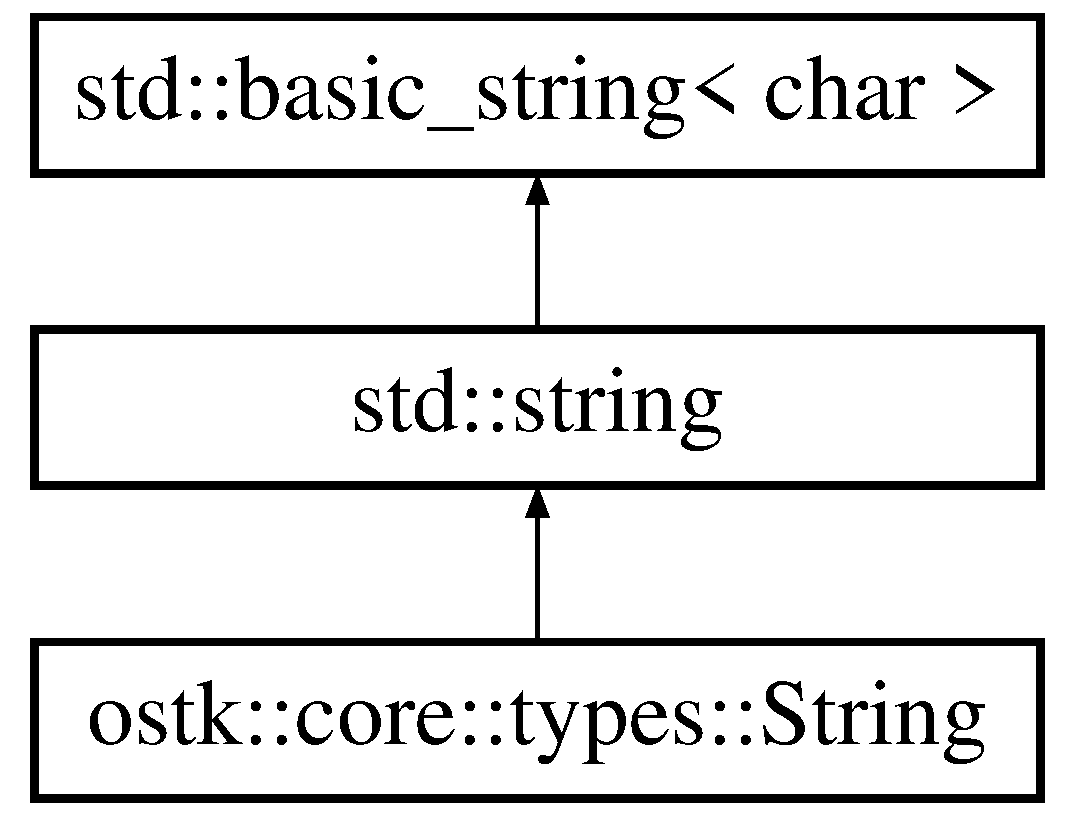
\includegraphics[height=3.000000cm]{classostk_1_1core_1_1types_1_1_string}
\end{center}
\end{figure}
\subsection*{Public Member Functions}
\begin{DoxyCompactItemize}
\item 
\hyperlink{classostk_1_1core_1_1types_1_1_string_a0f8e66f16108a449b1256c252c48ed3b}{String} ()
\item 
\hyperlink{classostk_1_1core_1_1types_1_1_string_aaaee3324b9d426284056794371932be5}{String} (const std\+::string \&a\+String)
\item 
\hyperlink{classostk_1_1core_1_1types_1_1_string_a9e8dd0b032ca07128968c7045158f0c4}{$\sim$\+String} ()
\item 
bool \hyperlink{classostk_1_1core_1_1types_1_1_string_abb04266529e07a89458cdd13516ff7cc}{is\+Empty} () const
\item 
bool \hyperlink{classostk_1_1core_1_1types_1_1_string_aae72dd9dba796952b935143d62b2b0a2}{is\+Uppercase} () const
\item 
bool \hyperlink{classostk_1_1core_1_1types_1_1_string_aab60cc8d552ebf3f32390af4a69af4ca}{is\+Lowercase} () const
\item 
bool \hyperlink{classostk_1_1core_1_1types_1_1_string_ac6fd01a3b12e86f08e61019799d8dc4d}{match} (const std\+::regex \&a\+Regular\+Expression) const
\begin{DoxyCompactList}\small\item\em Returns whether the string matches a regular expression. \end{DoxyCompactList}\item 
\hyperlink{namespaceostk_1_1core_1_1types_acf68f214a245e35a7c1994c84dc56746}{Size} \hyperlink{classostk_1_1core_1_1types_1_1_string_ab7529208a6f0acff749eb9a542b251d4}{get\+Length} () const
\item 
char \hyperlink{classostk_1_1core_1_1types_1_1_string_a54b1f561ed3634235d92f164e183db6f}{get\+First} () const
\item 
char \hyperlink{classostk_1_1core_1_1types_1_1_string_a9e2d1e808250b0987fae382912eb93d5}{get\+Last} () const
\item 
\hyperlink{classostk_1_1core_1_1types_1_1_string}{String} \hyperlink{classostk_1_1core_1_1types_1_1_string_a743124ed7378a1c6485621722216aed8}{get\+Head} (const \hyperlink{namespaceostk_1_1core_1_1types_acf68f214a245e35a7c1994c84dc56746}{Size} \&a\+Length) const
\item 
\hyperlink{classostk_1_1core_1_1types_1_1_string}{String} \hyperlink{classostk_1_1core_1_1types_1_1_string_aac6bc1ec037565caf85886b2e4177446}{get\+Tail} (const \hyperlink{namespaceostk_1_1core_1_1types_acf68f214a245e35a7c1994c84dc56746}{Size} \&a\+Length) const
\item 
\hyperlink{classostk_1_1core_1_1types_1_1_string}{String} \hyperlink{classostk_1_1core_1_1types_1_1_string_a9d0043c1313395defb939d47a6717107}{get\+Substring} (const \hyperlink{namespaceostk_1_1core_1_1types_a6e63c1b15b2e5bc87a43771c09fa913a}{Index} \&a\+Start\+Position, const \hyperlink{namespaceostk_1_1core_1_1types_acf68f214a245e35a7c1994c84dc56746}{Size} \&a\+Length) const
\item 
\hyperlink{classostk_1_1core_1_1types_1_1_string}{String} \& \hyperlink{classostk_1_1core_1_1types_1_1_string_a3fae6c7f00df2fb868949179fa20033e}{trim} ()
\begin{DoxyCompactList}\small\item\em Removes whitespace from both ends. \end{DoxyCompactList}\item 
\hyperlink{classostk_1_1core_1_1types_1_1_string}{String} \& \hyperlink{classostk_1_1core_1_1types_1_1_string_a69b7f8a58ee5a55636b0dfd5d8b85e2c}{replace} (const char a\+Character, const char a\+New\+Character)
\begin{DoxyCompactList}\small\item\em Replace all occurences of character by other character. \end{DoxyCompactList}\item 
\hyperlink{classostk_1_1core_1_1types_1_1_string}{String} \& \hyperlink{classostk_1_1core_1_1types_1_1_string_ae5c391a85f0fb05c1c6c4c62e3ce1fcd}{replace} (const \hyperlink{classostk_1_1core_1_1types_1_1_string}{String} \&a\+String, const \hyperlink{classostk_1_1core_1_1types_1_1_string}{String} \&a\+New\+String)
\begin{DoxyCompactList}\small\item\em Replace all occurences of string by other string. \end{DoxyCompactList}\end{DoxyCompactItemize}
\subsection*{Static Public Member Functions}
\begin{DoxyCompactItemize}
\item 
static \hyperlink{classostk_1_1core_1_1types_1_1_string}{String} \hyperlink{classostk_1_1core_1_1types_1_1_string_a66ebb081c6ece7e0140e355d0c6eaa23}{Empty} ()
\item 
static \hyperlink{classostk_1_1core_1_1types_1_1_string}{String} \hyperlink{classostk_1_1core_1_1types_1_1_string_a27a7c19665dd681777e092eff4c49495}{Boolean} (bool a\+Boolean)
\item 
static \hyperlink{classostk_1_1core_1_1types_1_1_string}{String} \hyperlink{classostk_1_1core_1_1types_1_1_string_a0aa76a29c15c07e068ecb1606f261712}{Char} (char a\+Character)
\item 
static \hyperlink{classostk_1_1core_1_1types_1_1_string}{String} \hyperlink{classostk_1_1core_1_1types_1_1_string_ace870e534ddbdfc01a56b849f7520c8c}{Replicate} (char a\+Character, \hyperlink{namespaceostk_1_1core_1_1types_acf68f214a245e35a7c1994c84dc56746}{Size} a\+Count)
\item 
static \hyperlink{classostk_1_1core_1_1types_1_1_string}{String} \hyperlink{classostk_1_1core_1_1types_1_1_string_afb3e7dae9340e7494ec875b6f65312d2}{Replicate} (const \hyperlink{classostk_1_1core_1_1types_1_1_string}{String} \&a\+String, \hyperlink{namespaceostk_1_1core_1_1types_acf68f214a245e35a7c1994c84dc56746}{Size} a\+Count)
\item 
{\footnotesize template$<$typename ... Args$>$ }\\static \hyperlink{classostk_1_1core_1_1types_1_1_string}{String} \hyperlink{classostk_1_1core_1_1types_1_1_string_afb00429ca478a722cd38904f52aa6f26}{Format} (const char $\ast$a\+Format, Args... an\+Argument\+List)
\begin{DoxyCompactList}\small\item\em Create formatted string. \end{DoxyCompactList}\end{DoxyCompactItemize}


\subsection{Detailed Description}
A sequence of characters. 

\begin{DoxyNote}{Note}
The current implementation (derived for std\+::string) is temporary, as this type of inheritance this is not recommended. 
\end{DoxyNote}


\subsection{Constructor \& Destructor Documentation}
\mbox{\Hypertarget{classostk_1_1core_1_1types_1_1_string_a0f8e66f16108a449b1256c252c48ed3b}\label{classostk_1_1core_1_1types_1_1_string_a0f8e66f16108a449b1256c252c48ed3b}} 
\index{ostk\+::core\+::types\+::\+String@{ostk\+::core\+::types\+::\+String}!String@{String}}
\index{String@{String}!ostk\+::core\+::types\+::\+String@{ostk\+::core\+::types\+::\+String}}
\subsubsection{\texorpdfstring{String()}{String()}\hspace{0.1cm}{\footnotesize\ttfamily [1/2]}}
{\footnotesize\ttfamily ostk\+::core\+::types\+::\+String\+::\+String (\begin{DoxyParamCaption}{ }\end{DoxyParamCaption})}

\mbox{\Hypertarget{classostk_1_1core_1_1types_1_1_string_aaaee3324b9d426284056794371932be5}\label{classostk_1_1core_1_1types_1_1_string_aaaee3324b9d426284056794371932be5}} 
\index{ostk\+::core\+::types\+::\+String@{ostk\+::core\+::types\+::\+String}!String@{String}}
\index{String@{String}!ostk\+::core\+::types\+::\+String@{ostk\+::core\+::types\+::\+String}}
\subsubsection{\texorpdfstring{String()}{String()}\hspace{0.1cm}{\footnotesize\ttfamily [2/2]}}
{\footnotesize\ttfamily ostk\+::core\+::types\+::\+String\+::\+String (\begin{DoxyParamCaption}\item[{const std\+::string \&}]{a\+String }\end{DoxyParamCaption})}

\mbox{\Hypertarget{classostk_1_1core_1_1types_1_1_string_a9e8dd0b032ca07128968c7045158f0c4}\label{classostk_1_1core_1_1types_1_1_string_a9e8dd0b032ca07128968c7045158f0c4}} 
\index{ostk\+::core\+::types\+::\+String@{ostk\+::core\+::types\+::\+String}!````~String@{$\sim$\+String}}
\index{````~String@{$\sim$\+String}!ostk\+::core\+::types\+::\+String@{ostk\+::core\+::types\+::\+String}}
\subsubsection{\texorpdfstring{$\sim$\+String()}{~String()}}
{\footnotesize\ttfamily ostk\+::core\+::types\+::\+String\+::$\sim$\+String (\begin{DoxyParamCaption}{ }\end{DoxyParamCaption})}



\subsection{Member Function Documentation}
\mbox{\Hypertarget{classostk_1_1core_1_1types_1_1_string_a27a7c19665dd681777e092eff4c49495}\label{classostk_1_1core_1_1types_1_1_string_a27a7c19665dd681777e092eff4c49495}} 
\index{ostk\+::core\+::types\+::\+String@{ostk\+::core\+::types\+::\+String}!Boolean@{Boolean}}
\index{Boolean@{Boolean}!ostk\+::core\+::types\+::\+String@{ostk\+::core\+::types\+::\+String}}
\subsubsection{\texorpdfstring{Boolean()}{Boolean()}}
{\footnotesize\ttfamily \hyperlink{classostk_1_1core_1_1types_1_1_string}{String} ostk\+::core\+::types\+::\+String\+::\+Boolean (\begin{DoxyParamCaption}\item[{bool}]{a\+Boolean }\end{DoxyParamCaption})\hspace{0.3cm}{\ttfamily [static]}}

\mbox{\Hypertarget{classostk_1_1core_1_1types_1_1_string_a0aa76a29c15c07e068ecb1606f261712}\label{classostk_1_1core_1_1types_1_1_string_a0aa76a29c15c07e068ecb1606f261712}} 
\index{ostk\+::core\+::types\+::\+String@{ostk\+::core\+::types\+::\+String}!Char@{Char}}
\index{Char@{Char}!ostk\+::core\+::types\+::\+String@{ostk\+::core\+::types\+::\+String}}
\subsubsection{\texorpdfstring{Char()}{Char()}}
{\footnotesize\ttfamily \hyperlink{classostk_1_1core_1_1types_1_1_string}{String} ostk\+::core\+::types\+::\+String\+::\+Char (\begin{DoxyParamCaption}\item[{char}]{a\+Character }\end{DoxyParamCaption})\hspace{0.3cm}{\ttfamily [static]}}

\mbox{\Hypertarget{classostk_1_1core_1_1types_1_1_string_a66ebb081c6ece7e0140e355d0c6eaa23}\label{classostk_1_1core_1_1types_1_1_string_a66ebb081c6ece7e0140e355d0c6eaa23}} 
\index{ostk\+::core\+::types\+::\+String@{ostk\+::core\+::types\+::\+String}!Empty@{Empty}}
\index{Empty@{Empty}!ostk\+::core\+::types\+::\+String@{ostk\+::core\+::types\+::\+String}}
\subsubsection{\texorpdfstring{Empty()}{Empty()}}
{\footnotesize\ttfamily \hyperlink{classostk_1_1core_1_1types_1_1_string}{String} ostk\+::core\+::types\+::\+String\+::\+Empty (\begin{DoxyParamCaption}{ }\end{DoxyParamCaption})\hspace{0.3cm}{\ttfamily [static]}}

\mbox{\Hypertarget{classostk_1_1core_1_1types_1_1_string_afb00429ca478a722cd38904f52aa6f26}\label{classostk_1_1core_1_1types_1_1_string_afb00429ca478a722cd38904f52aa6f26}} 
\index{ostk\+::core\+::types\+::\+String@{ostk\+::core\+::types\+::\+String}!Format@{Format}}
\index{Format@{Format}!ostk\+::core\+::types\+::\+String@{ostk\+::core\+::types\+::\+String}}
\subsubsection{\texorpdfstring{Format()}{Format()}}
{\footnotesize\ttfamily template$<$typename ... Args$>$ \\
static \hyperlink{classostk_1_1core_1_1types_1_1_string}{String} ostk\+::core\+::types\+::\+String\+::\+Format (\begin{DoxyParamCaption}\item[{const char $\ast$}]{a\+Format,  }\item[{Args...}]{an\+Argument\+List }\end{DoxyParamCaption})\hspace{0.3cm}{\ttfamily [inline]}, {\ttfamily [static]}}



Create formatted string. 


\begin{DoxyCode}
\hyperlink{classostk_1_1core_1_1types_1_1_string_afb00429ca478a722cd38904f52aa6f26}{String::Format}(\textcolor{stringliteral}{"\{0\}, \{1\}!"}, \textcolor{stringliteral}{"Hello"}, \textcolor{stringliteral}{"World"}) ; \textcolor{comment}{// "Hello, World!"}
\hyperlink{classostk_1_1core_1_1types_1_1_string_afb00429ca478a722cd38904f52aa6f26}{String::Format}(\textcolor{stringliteral}{"Let's operate \{0\} \{1\}!"}, 123, \textcolor{stringliteral}{"satellites"}) ; \textcolor{comment}{// "Let's operate 123
       satellites!"}
\end{DoxyCode}



\begin{DoxyParams}[1]{Parameters}
\mbox{\tt in}  & {\em a\+Format} & A format \\
\hline
\mbox{\tt in}  & {\em an\+Argument\+List} & A list of arguments \\
\hline
\end{DoxyParams}
\begin{DoxyReturn}{Returns}
Formatted string 
\end{DoxyReturn}
\mbox{\Hypertarget{classostk_1_1core_1_1types_1_1_string_a54b1f561ed3634235d92f164e183db6f}\label{classostk_1_1core_1_1types_1_1_string_a54b1f561ed3634235d92f164e183db6f}} 
\index{ostk\+::core\+::types\+::\+String@{ostk\+::core\+::types\+::\+String}!get\+First@{get\+First}}
\index{get\+First@{get\+First}!ostk\+::core\+::types\+::\+String@{ostk\+::core\+::types\+::\+String}}
\subsubsection{\texorpdfstring{get\+First()}{getFirst()}}
{\footnotesize\ttfamily char ostk\+::core\+::types\+::\+String\+::get\+First (\begin{DoxyParamCaption}{ }\end{DoxyParamCaption}) const}

\mbox{\Hypertarget{classostk_1_1core_1_1types_1_1_string_a743124ed7378a1c6485621722216aed8}\label{classostk_1_1core_1_1types_1_1_string_a743124ed7378a1c6485621722216aed8}} 
\index{ostk\+::core\+::types\+::\+String@{ostk\+::core\+::types\+::\+String}!get\+Head@{get\+Head}}
\index{get\+Head@{get\+Head}!ostk\+::core\+::types\+::\+String@{ostk\+::core\+::types\+::\+String}}
\subsubsection{\texorpdfstring{get\+Head()}{getHead()}}
{\footnotesize\ttfamily \hyperlink{classostk_1_1core_1_1types_1_1_string}{String} ostk\+::core\+::types\+::\+String\+::get\+Head (\begin{DoxyParamCaption}\item[{const \hyperlink{namespaceostk_1_1core_1_1types_acf68f214a245e35a7c1994c84dc56746}{Size} \&}]{a\+Length }\end{DoxyParamCaption}) const}

\mbox{\Hypertarget{classostk_1_1core_1_1types_1_1_string_a9e2d1e808250b0987fae382912eb93d5}\label{classostk_1_1core_1_1types_1_1_string_a9e2d1e808250b0987fae382912eb93d5}} 
\index{ostk\+::core\+::types\+::\+String@{ostk\+::core\+::types\+::\+String}!get\+Last@{get\+Last}}
\index{get\+Last@{get\+Last}!ostk\+::core\+::types\+::\+String@{ostk\+::core\+::types\+::\+String}}
\subsubsection{\texorpdfstring{get\+Last()}{getLast()}}
{\footnotesize\ttfamily char ostk\+::core\+::types\+::\+String\+::get\+Last (\begin{DoxyParamCaption}{ }\end{DoxyParamCaption}) const}

\mbox{\Hypertarget{classostk_1_1core_1_1types_1_1_string_ab7529208a6f0acff749eb9a542b251d4}\label{classostk_1_1core_1_1types_1_1_string_ab7529208a6f0acff749eb9a542b251d4}} 
\index{ostk\+::core\+::types\+::\+String@{ostk\+::core\+::types\+::\+String}!get\+Length@{get\+Length}}
\index{get\+Length@{get\+Length}!ostk\+::core\+::types\+::\+String@{ostk\+::core\+::types\+::\+String}}
\subsubsection{\texorpdfstring{get\+Length()}{getLength()}}
{\footnotesize\ttfamily \hyperlink{namespaceostk_1_1core_1_1types_acf68f214a245e35a7c1994c84dc56746}{Size} ostk\+::core\+::types\+::\+String\+::get\+Length (\begin{DoxyParamCaption}{ }\end{DoxyParamCaption}) const}

\mbox{\Hypertarget{classostk_1_1core_1_1types_1_1_string_a9d0043c1313395defb939d47a6717107}\label{classostk_1_1core_1_1types_1_1_string_a9d0043c1313395defb939d47a6717107}} 
\index{ostk\+::core\+::types\+::\+String@{ostk\+::core\+::types\+::\+String}!get\+Substring@{get\+Substring}}
\index{get\+Substring@{get\+Substring}!ostk\+::core\+::types\+::\+String@{ostk\+::core\+::types\+::\+String}}
\subsubsection{\texorpdfstring{get\+Substring()}{getSubstring()}}
{\footnotesize\ttfamily \hyperlink{classostk_1_1core_1_1types_1_1_string}{String} ostk\+::core\+::types\+::\+String\+::get\+Substring (\begin{DoxyParamCaption}\item[{const \hyperlink{namespaceostk_1_1core_1_1types_a6e63c1b15b2e5bc87a43771c09fa913a}{Index} \&}]{a\+Start\+Position,  }\item[{const \hyperlink{namespaceostk_1_1core_1_1types_acf68f214a245e35a7c1994c84dc56746}{Size} \&}]{a\+Length }\end{DoxyParamCaption}) const}

\mbox{\Hypertarget{classostk_1_1core_1_1types_1_1_string_aac6bc1ec037565caf85886b2e4177446}\label{classostk_1_1core_1_1types_1_1_string_aac6bc1ec037565caf85886b2e4177446}} 
\index{ostk\+::core\+::types\+::\+String@{ostk\+::core\+::types\+::\+String}!get\+Tail@{get\+Tail}}
\index{get\+Tail@{get\+Tail}!ostk\+::core\+::types\+::\+String@{ostk\+::core\+::types\+::\+String}}
\subsubsection{\texorpdfstring{get\+Tail()}{getTail()}}
{\footnotesize\ttfamily \hyperlink{classostk_1_1core_1_1types_1_1_string}{String} ostk\+::core\+::types\+::\+String\+::get\+Tail (\begin{DoxyParamCaption}\item[{const \hyperlink{namespaceostk_1_1core_1_1types_acf68f214a245e35a7c1994c84dc56746}{Size} \&}]{a\+Length }\end{DoxyParamCaption}) const}

\mbox{\Hypertarget{classostk_1_1core_1_1types_1_1_string_abb04266529e07a89458cdd13516ff7cc}\label{classostk_1_1core_1_1types_1_1_string_abb04266529e07a89458cdd13516ff7cc}} 
\index{ostk\+::core\+::types\+::\+String@{ostk\+::core\+::types\+::\+String}!is\+Empty@{is\+Empty}}
\index{is\+Empty@{is\+Empty}!ostk\+::core\+::types\+::\+String@{ostk\+::core\+::types\+::\+String}}
\subsubsection{\texorpdfstring{is\+Empty()}{isEmpty()}}
{\footnotesize\ttfamily bool ostk\+::core\+::types\+::\+String\+::is\+Empty (\begin{DoxyParamCaption}{ }\end{DoxyParamCaption}) const}

\mbox{\Hypertarget{classostk_1_1core_1_1types_1_1_string_aab60cc8d552ebf3f32390af4a69af4ca}\label{classostk_1_1core_1_1types_1_1_string_aab60cc8d552ebf3f32390af4a69af4ca}} 
\index{ostk\+::core\+::types\+::\+String@{ostk\+::core\+::types\+::\+String}!is\+Lowercase@{is\+Lowercase}}
\index{is\+Lowercase@{is\+Lowercase}!ostk\+::core\+::types\+::\+String@{ostk\+::core\+::types\+::\+String}}
\subsubsection{\texorpdfstring{is\+Lowercase()}{isLowercase()}}
{\footnotesize\ttfamily bool ostk\+::core\+::types\+::\+String\+::is\+Lowercase (\begin{DoxyParamCaption}{ }\end{DoxyParamCaption}) const}

\mbox{\Hypertarget{classostk_1_1core_1_1types_1_1_string_aae72dd9dba796952b935143d62b2b0a2}\label{classostk_1_1core_1_1types_1_1_string_aae72dd9dba796952b935143d62b2b0a2}} 
\index{ostk\+::core\+::types\+::\+String@{ostk\+::core\+::types\+::\+String}!is\+Uppercase@{is\+Uppercase}}
\index{is\+Uppercase@{is\+Uppercase}!ostk\+::core\+::types\+::\+String@{ostk\+::core\+::types\+::\+String}}
\subsubsection{\texorpdfstring{is\+Uppercase()}{isUppercase()}}
{\footnotesize\ttfamily bool ostk\+::core\+::types\+::\+String\+::is\+Uppercase (\begin{DoxyParamCaption}{ }\end{DoxyParamCaption}) const}

\mbox{\Hypertarget{classostk_1_1core_1_1types_1_1_string_ac6fd01a3b12e86f08e61019799d8dc4d}\label{classostk_1_1core_1_1types_1_1_string_ac6fd01a3b12e86f08e61019799d8dc4d}} 
\index{ostk\+::core\+::types\+::\+String@{ostk\+::core\+::types\+::\+String}!match@{match}}
\index{match@{match}!ostk\+::core\+::types\+::\+String@{ostk\+::core\+::types\+::\+String}}
\subsubsection{\texorpdfstring{match()}{match()}}
{\footnotesize\ttfamily bool ostk\+::core\+::types\+::\+String\+::match (\begin{DoxyParamCaption}\item[{const std\+::regex \&}]{a\+Regular\+Expression }\end{DoxyParamCaption}) const}



Returns whether the string matches a regular expression. 


\begin{DoxyCode}
\hyperlink{classostk_1_1core_1_1types_1_1_string_a0f8e66f16108a449b1256c252c48ed3b}{String}(\textcolor{stringliteral}{"abc"}).match(std::regex(\textcolor{stringliteral}{"^[a-z]\{3\}$"})) ; \textcolor{comment}{// True}
\end{DoxyCode}



\begin{DoxyParams}[1]{Parameters}
\mbox{\tt in}  & {\em a\+Regular\+Expression} & A regular expression \\
\hline
\end{DoxyParams}
\begin{DoxyReturn}{Returns}
True if matches regular expression 
\end{DoxyReturn}
\mbox{\Hypertarget{classostk_1_1core_1_1types_1_1_string_a69b7f8a58ee5a55636b0dfd5d8b85e2c}\label{classostk_1_1core_1_1types_1_1_string_a69b7f8a58ee5a55636b0dfd5d8b85e2c}} 
\index{ostk\+::core\+::types\+::\+String@{ostk\+::core\+::types\+::\+String}!replace@{replace}}
\index{replace@{replace}!ostk\+::core\+::types\+::\+String@{ostk\+::core\+::types\+::\+String}}
\subsubsection{\texorpdfstring{replace()}{replace()}\hspace{0.1cm}{\footnotesize\ttfamily [1/2]}}
{\footnotesize\ttfamily \hyperlink{classostk_1_1core_1_1types_1_1_string}{String} \& ostk\+::core\+::types\+::\+String\+::replace (\begin{DoxyParamCaption}\item[{const char}]{a\+Character,  }\item[{const char}]{a\+New\+Character }\end{DoxyParamCaption})}



Replace all occurences of character by other character. 


\begin{DoxyParams}[1]{Parameters}
\mbox{\tt in}  & {\em a\+Character} & A character \\
\hline
\mbox{\tt in}  & {\em a\+New\+Character} & A replacement character \\
\hline
\end{DoxyParams}
\begin{DoxyReturn}{Returns}
Reference to string 
\end{DoxyReturn}
\mbox{\Hypertarget{classostk_1_1core_1_1types_1_1_string_ae5c391a85f0fb05c1c6c4c62e3ce1fcd}\label{classostk_1_1core_1_1types_1_1_string_ae5c391a85f0fb05c1c6c4c62e3ce1fcd}} 
\index{ostk\+::core\+::types\+::\+String@{ostk\+::core\+::types\+::\+String}!replace@{replace}}
\index{replace@{replace}!ostk\+::core\+::types\+::\+String@{ostk\+::core\+::types\+::\+String}}
\subsubsection{\texorpdfstring{replace()}{replace()}\hspace{0.1cm}{\footnotesize\ttfamily [2/2]}}
{\footnotesize\ttfamily \hyperlink{classostk_1_1core_1_1types_1_1_string}{String} \& ostk\+::core\+::types\+::\+String\+::replace (\begin{DoxyParamCaption}\item[{const \hyperlink{classostk_1_1core_1_1types_1_1_string}{String} \&}]{a\+String,  }\item[{const \hyperlink{classostk_1_1core_1_1types_1_1_string}{String} \&}]{a\+New\+String }\end{DoxyParamCaption})}



Replace all occurences of string by other string. 


\begin{DoxyParams}[1]{Parameters}
\mbox{\tt in}  & {\em a\+Character} & A string \\
\hline
\mbox{\tt in}  & {\em a\+New\+Character} & A replacement string \\
\hline
\end{DoxyParams}
\begin{DoxyReturn}{Returns}
Reference to string 
\end{DoxyReturn}
\mbox{\Hypertarget{classostk_1_1core_1_1types_1_1_string_ace870e534ddbdfc01a56b849f7520c8c}\label{classostk_1_1core_1_1types_1_1_string_ace870e534ddbdfc01a56b849f7520c8c}} 
\index{ostk\+::core\+::types\+::\+String@{ostk\+::core\+::types\+::\+String}!Replicate@{Replicate}}
\index{Replicate@{Replicate}!ostk\+::core\+::types\+::\+String@{ostk\+::core\+::types\+::\+String}}
\subsubsection{\texorpdfstring{Replicate()}{Replicate()}\hspace{0.1cm}{\footnotesize\ttfamily [1/2]}}
{\footnotesize\ttfamily \hyperlink{classostk_1_1core_1_1types_1_1_string}{String} ostk\+::core\+::types\+::\+String\+::\+Replicate (\begin{DoxyParamCaption}\item[{char}]{a\+Character,  }\item[{\hyperlink{namespaceostk_1_1core_1_1types_acf68f214a245e35a7c1994c84dc56746}{Size}}]{a\+Count }\end{DoxyParamCaption})\hspace{0.3cm}{\ttfamily [static]}}

\mbox{\Hypertarget{classostk_1_1core_1_1types_1_1_string_afb3e7dae9340e7494ec875b6f65312d2}\label{classostk_1_1core_1_1types_1_1_string_afb3e7dae9340e7494ec875b6f65312d2}} 
\index{ostk\+::core\+::types\+::\+String@{ostk\+::core\+::types\+::\+String}!Replicate@{Replicate}}
\index{Replicate@{Replicate}!ostk\+::core\+::types\+::\+String@{ostk\+::core\+::types\+::\+String}}
\subsubsection{\texorpdfstring{Replicate()}{Replicate()}\hspace{0.1cm}{\footnotesize\ttfamily [2/2]}}
{\footnotesize\ttfamily \hyperlink{classostk_1_1core_1_1types_1_1_string}{String} ostk\+::core\+::types\+::\+String\+::\+Replicate (\begin{DoxyParamCaption}\item[{const \hyperlink{classostk_1_1core_1_1types_1_1_string}{String} \&}]{a\+String,  }\item[{\hyperlink{namespaceostk_1_1core_1_1types_acf68f214a245e35a7c1994c84dc56746}{Size}}]{a\+Count }\end{DoxyParamCaption})\hspace{0.3cm}{\ttfamily [static]}}

\mbox{\Hypertarget{classostk_1_1core_1_1types_1_1_string_a3fae6c7f00df2fb868949179fa20033e}\label{classostk_1_1core_1_1types_1_1_string_a3fae6c7f00df2fb868949179fa20033e}} 
\index{ostk\+::core\+::types\+::\+String@{ostk\+::core\+::types\+::\+String}!trim@{trim}}
\index{trim@{trim}!ostk\+::core\+::types\+::\+String@{ostk\+::core\+::types\+::\+String}}
\subsubsection{\texorpdfstring{trim()}{trim()}}
{\footnotesize\ttfamily \hyperlink{classostk_1_1core_1_1types_1_1_string}{String} \& ostk\+::core\+::types\+::\+String\+::trim (\begin{DoxyParamCaption}{ }\end{DoxyParamCaption})}



Removes whitespace from both ends. 

\begin{DoxyReturn}{Returns}
Reference to string 
\end{DoxyReturn}


The documentation for this class was generated from the following files\+:\begin{DoxyCompactItemize}
\item 
include/\+Open\+Space\+Toolkit/\+Core/\+Types/\hyperlink{_string_8hpp}{String.\+hpp}\item 
src/\+Open\+Space\+Toolkit/\+Core/\+Types/\hyperlink{_string_8cpp}{String.\+cpp}\end{DoxyCompactItemize}

\hypertarget{classostk_1_1core_1_1ctnr_1_1_table}{}\section{ostk\+:\+:core\+:\+:ctnr\+:\+:Table Class Reference}
\label{classostk_1_1core_1_1ctnr_1_1_table}\index{ostk\+::core\+::ctnr\+::\+Table@{ostk\+::core\+::ctnr\+::\+Table}}


\hyperlink{classostk_1_1core_1_1ctnr_1_1_table}{Table} container.  




{\ttfamily \#include $<$Table.\+hpp$>$}

\subsection*{Public Types}
\begin{DoxyCompactItemize}
\item 
enum \hyperlink{classostk_1_1core_1_1ctnr_1_1_table_aacb867db63d74cac28a388029bf161d2}{Format} \{ \hyperlink{classostk_1_1core_1_1ctnr_1_1_table_aacb867db63d74cac28a388029bf161d2aec0fc0100c4fc1ce4eea230c3dc10360}{Format\+::\+Undefined}, 
\hyperlink{classostk_1_1core_1_1ctnr_1_1_table_aacb867db63d74cac28a388029bf161d2acc8d68c551c4a9a6d5313e07de4deafd}{Format\+::\+C\+SV}
 \}\begin{DoxyCompactList}\small\item\em \hyperlink{classostk_1_1core_1_1ctnr_1_1_table}{Table} format. \end{DoxyCompactList}
\item 
typedef \hyperlink{classostk_1_1core_1_1ctnr_1_1_array}{Array}$<$ \hyperlink{classostk_1_1core_1_1ctnr_1_1table_1_1_row}{Row} $>$\+::\hyperlink{classostk_1_1core_1_1ctnr_1_1_table_a44e6a375120737f0675ea6689022050f}{Const\+Iterator} \hyperlink{classostk_1_1core_1_1ctnr_1_1_table_a44e6a375120737f0675ea6689022050f}{Const\+Iterator}
\begin{DoxyCompactList}\small\item\em \hyperlink{classostk_1_1core_1_1ctnr_1_1_table}{Table} constant iterator. \end{DoxyCompactList}\end{DoxyCompactItemize}
\subsection*{Public Member Functions}
\begin{DoxyCompactItemize}
\item 
\hyperlink{classostk_1_1core_1_1ctnr_1_1_table_a1b799fa804faf23f9dd4905df90a5cd7}{Table} (const \hyperlink{classostk_1_1core_1_1ctnr_1_1_array}{Array}$<$ \hyperlink{classostk_1_1core_1_1types_1_1_string}{String} $>$ \&a\+Header, const \hyperlink{classostk_1_1core_1_1ctnr_1_1_array}{Array}$<$ \hyperlink{classostk_1_1core_1_1ctnr_1_1table_1_1_row}{Row} $>$ \&a\+Row\+Array)
\begin{DoxyCompactList}\small\item\em Constructor. \end{DoxyCompactList}\item 
\hyperlink{classostk_1_1core_1_1ctnr_1_1_table_a165db4eb20ff95886daded2766b090ad}{Table} (const \hyperlink{classostk_1_1core_1_1ctnr_1_1_array}{Array}$<$ \hyperlink{classostk_1_1core_1_1types_1_1_string}{String} $>$ \&a\+Header)
\begin{DoxyCompactList}\small\item\em Constructor. \end{DoxyCompactList}\item 
\hyperlink{classostk_1_1core_1_1ctnr_1_1_table_a94c2705ce991b21927a86bce4f3d6dce}{Table} (const \hyperlink{classostk_1_1core_1_1ctnr_1_1_table}{Table} \&a\+Table)
\begin{DoxyCompactList}\small\item\em Copy constructor. \end{DoxyCompactList}\item 
\hyperlink{classostk_1_1core_1_1ctnr_1_1_table}{Table} \& \hyperlink{classostk_1_1core_1_1ctnr_1_1_table_a5b1517b597097ffc09293208191f4a3b}{operator=} (const \hyperlink{classostk_1_1core_1_1ctnr_1_1_table}{Table} \&a\+Table)
\begin{DoxyCompactList}\small\item\em Copy assignment operator. \end{DoxyCompactList}\item 
bool \hyperlink{classostk_1_1core_1_1ctnr_1_1_table_afc0baa8593eaa0c3720c098e7bfdfe3a}{operator==} (const \hyperlink{classostk_1_1core_1_1ctnr_1_1_table}{Table} \&a\+Table) const
\begin{DoxyCompactList}\small\item\em Equal to operator. \end{DoxyCompactList}\item 
bool \hyperlink{classostk_1_1core_1_1ctnr_1_1_table_a40d74d8b1bead3b99b349c65f3d377cb}{operator!=} (const \hyperlink{classostk_1_1core_1_1ctnr_1_1_table}{Table} \&a\+Table) const
\begin{DoxyCompactList}\small\item\em Not equal to operator. \end{DoxyCompactList}\item 
const \hyperlink{classostk_1_1core_1_1ctnr_1_1table_1_1_row}{Row} \& \hyperlink{classostk_1_1core_1_1ctnr_1_1_table_a7195c6f21811425473ecabfc5cc0340c}{operator\mbox{[}$\,$\mbox{]}} (const Index \&a\+Row\+Index) const
\begin{DoxyCompactList}\small\item\em Subscript operator (row accessor) \end{DoxyCompactList}\item 
const Cell \& \hyperlink{classostk_1_1core_1_1ctnr_1_1_table_aad3fbcecb674916cf50d0388031156a7}{operator()} (const Index \&a\+Row\+Index, const Index \&a\+Column\+Index) const
\begin{DoxyCompactList}\small\item\em Function call operator (cell accessor) \end{DoxyCompactList}\item 
const Cell \& \hyperlink{classostk_1_1core_1_1ctnr_1_1_table_ab86f822abd7641711455bb963cc61767}{operator()} (const Index \&a\+Row\+Index, const \hyperlink{classostk_1_1core_1_1types_1_1_string}{String} \&a\+Column\+Name) const
\begin{DoxyCompactList}\small\item\em Function call operator (cell accessor) \end{DoxyCompactList}\item 
bool \hyperlink{classostk_1_1core_1_1ctnr_1_1_table_a8e56fe6a310edb33ea1cbc69c2609ee0}{is\+Empty} () const
\begin{DoxyCompactList}\small\item\em Check if table is empty. \end{DoxyCompactList}\item 
bool \hyperlink{classostk_1_1core_1_1ctnr_1_1_table_a4c68a783ba37aa13d3b5802dd72a442d}{has\+Column\+With\+Name} (const \hyperlink{classostk_1_1core_1_1types_1_1_string}{String} \&a\+Column\+Name) const
\begin{DoxyCompactList}\small\item\em Returns true is table has column with a given name. \end{DoxyCompactList}\item 
Size \hyperlink{classostk_1_1core_1_1ctnr_1_1_table_abe8c76eb8d3efed7c548b2112c3ba228}{get\+Row\+Count} () const
\begin{DoxyCompactList}\small\item\em Get number of rows. \end{DoxyCompactList}\item 
Size \hyperlink{classostk_1_1core_1_1ctnr_1_1_table_ae06b81ee41dfc025d414c4bc7e6c7808}{get\+Column\+Count} () const
\begin{DoxyCompactList}\small\item\em Get number of columns. \end{DoxyCompactList}\item 
Index \hyperlink{classostk_1_1core_1_1ctnr_1_1_table_aa778da3685c788f96eeddc7eb870581a}{get\+Index\+Of\+Column\+With\+Name} (const \hyperlink{classostk_1_1core_1_1types_1_1_string}{String} \&a\+Column\+Name) const
\begin{DoxyCompactList}\small\item\em Returns the index of column with a given name. \end{DoxyCompactList}\item 
void \hyperlink{classostk_1_1core_1_1ctnr_1_1_table_a10f2a23e9bdf2e34ab0b938c40cd1d66}{add\+Row} (const \hyperlink{classostk_1_1core_1_1ctnr_1_1table_1_1_row}{Row} \&a\+Row)
\begin{DoxyCompactList}\small\item\em Add row. \end{DoxyCompactList}\item 
void \hyperlink{classostk_1_1core_1_1ctnr_1_1_table_ad373553dd3803cde127ccdafe540456c}{clear} ()
\begin{DoxyCompactList}\small\item\em Clear table. \end{DoxyCompactList}\item 
\hyperlink{classostk_1_1core_1_1ctnr_1_1_table_a44e6a375120737f0675ea6689022050f}{Table\+::\+Const\+Iterator} \hyperlink{classostk_1_1core_1_1ctnr_1_1_table_a0d4c71fa820c4381bd893bde8a0c8e45}{begin} () const
\begin{DoxyCompactList}\small\item\em Get begin constant interator. \end{DoxyCompactList}\item 
\hyperlink{classostk_1_1core_1_1ctnr_1_1_table_a44e6a375120737f0675ea6689022050f}{Table\+::\+Const\+Iterator} \hyperlink{classostk_1_1core_1_1ctnr_1_1_table_a0c7c2095ac2a834b689e16a49b2f001a}{end} () const
\begin{DoxyCompactList}\small\item\em Get end constant interator. \end{DoxyCompactList}\end{DoxyCompactItemize}
\subsection*{Static Public Member Functions}
\begin{DoxyCompactItemize}
\item 
static \hyperlink{classostk_1_1core_1_1ctnr_1_1_table}{Table} \hyperlink{classostk_1_1core_1_1ctnr_1_1_table_af7ec9c84859ac8809021556c1c26dd8b}{Empty} ()
\begin{DoxyCompactList}\small\item\em Constructs an empty table. \end{DoxyCompactList}\item 
static \hyperlink{classostk_1_1core_1_1ctnr_1_1_table}{Table} \hyperlink{classostk_1_1core_1_1ctnr_1_1_table_a0bf37edce9a3680aad444469f813a099}{Load} (const \hyperlink{classostk_1_1core_1_1fs_1_1_file}{File} \&a\+File, const \hyperlink{classostk_1_1core_1_1ctnr_1_1_table_aacb867db63d74cac28a388029bf161d2}{Table\+::\+Format} \&a\+Format=\hyperlink{classostk_1_1core_1_1ctnr_1_1_table_aacb867db63d74cac28a388029bf161d2aec0fc0100c4fc1ce4eea230c3dc10360}{Table\+::\+Format\+::\+Undefined}, bool has\+Header=true)
\begin{DoxyCompactList}\small\item\em Constructs a table from a file. \end{DoxyCompactList}\end{DoxyCompactItemize}
\subsection*{Friends}
\begin{DoxyCompactItemize}
\item 
std\+::ostream \& \hyperlink{classostk_1_1core_1_1ctnr_1_1_table_afaece709b2f143e4011941ae67b7adba}{operator$<$$<$} (std\+::ostream \&an\+Output\+Stream, const \hyperlink{classostk_1_1core_1_1ctnr_1_1_table}{Table} \&a\+Table)
\begin{DoxyCompactList}\small\item\em Output stream operator. \end{DoxyCompactList}\end{DoxyCompactItemize}


\subsection{Detailed Description}
\hyperlink{classostk_1_1core_1_1ctnr_1_1_table}{Table} container. 

\subsection{Member Typedef Documentation}
\mbox{\Hypertarget{classostk_1_1core_1_1ctnr_1_1_table_a44e6a375120737f0675ea6689022050f}\label{classostk_1_1core_1_1ctnr_1_1_table_a44e6a375120737f0675ea6689022050f}} 
\index{ostk\+::core\+::ctnr\+::\+Table@{ostk\+::core\+::ctnr\+::\+Table}!Const\+Iterator@{Const\+Iterator}}
\index{Const\+Iterator@{Const\+Iterator}!ostk\+::core\+::ctnr\+::\+Table@{ostk\+::core\+::ctnr\+::\+Table}}
\subsubsection{\texorpdfstring{Const\+Iterator}{ConstIterator}}
{\footnotesize\ttfamily typedef \hyperlink{classostk_1_1core_1_1ctnr_1_1_array}{Array}$<$\hyperlink{classostk_1_1core_1_1ctnr_1_1table_1_1_row}{Row}$>$\+::\hyperlink{classostk_1_1core_1_1ctnr_1_1_table_a44e6a375120737f0675ea6689022050f}{Const\+Iterator} \hyperlink{classostk_1_1core_1_1ctnr_1_1_table_a44e6a375120737f0675ea6689022050f}{ostk\+::core\+::ctnr\+::\+Table\+::\+Const\+Iterator}}



\hyperlink{classostk_1_1core_1_1ctnr_1_1_table}{Table} constant iterator. 



\subsection{Member Enumeration Documentation}
\mbox{\Hypertarget{classostk_1_1core_1_1ctnr_1_1_table_aacb867db63d74cac28a388029bf161d2}\label{classostk_1_1core_1_1ctnr_1_1_table_aacb867db63d74cac28a388029bf161d2}} 
\index{ostk\+::core\+::ctnr\+::\+Table@{ostk\+::core\+::ctnr\+::\+Table}!Format@{Format}}
\index{Format@{Format}!ostk\+::core\+::ctnr\+::\+Table@{ostk\+::core\+::ctnr\+::\+Table}}
\subsubsection{\texorpdfstring{Format}{Format}}
{\footnotesize\ttfamily enum \hyperlink{classostk_1_1core_1_1ctnr_1_1_table_aacb867db63d74cac28a388029bf161d2}{ostk\+::core\+::ctnr\+::\+Table\+::\+Format}\hspace{0.3cm}{\ttfamily [strong]}}



\hyperlink{classostk_1_1core_1_1ctnr_1_1_table}{Table} format. 

\begin{DoxyEnumFields}{Enumerator}
\raisebox{\heightof{T}}[0pt][0pt]{\index{Undefined@{Undefined}!ostk\+::core\+::ctnr\+::\+Table@{ostk\+::core\+::ctnr\+::\+Table}}\index{ostk\+::core\+::ctnr\+::\+Table@{ostk\+::core\+::ctnr\+::\+Table}!Undefined@{Undefined}}}\mbox{\Hypertarget{classostk_1_1core_1_1ctnr_1_1_table_aacb867db63d74cac28a388029bf161d2aec0fc0100c4fc1ce4eea230c3dc10360}\label{classostk_1_1core_1_1ctnr_1_1_table_aacb867db63d74cac28a388029bf161d2aec0fc0100c4fc1ce4eea230c3dc10360}} 
Undefined&Undefined format. \\
\hline

\raisebox{\heightof{T}}[0pt][0pt]{\index{C\+SV@{C\+SV}!ostk\+::core\+::ctnr\+::\+Table@{ostk\+::core\+::ctnr\+::\+Table}}\index{ostk\+::core\+::ctnr\+::\+Table@{ostk\+::core\+::ctnr\+::\+Table}!C\+SV@{C\+SV}}}\mbox{\Hypertarget{classostk_1_1core_1_1ctnr_1_1_table_aacb867db63d74cac28a388029bf161d2acc8d68c551c4a9a6d5313e07de4deafd}\label{classostk_1_1core_1_1ctnr_1_1_table_aacb867db63d74cac28a388029bf161d2acc8d68c551c4a9a6d5313e07de4deafd}} 
C\+SV&Comma-\/\+Separated Values format. \\
\hline

\end{DoxyEnumFields}


\subsection{Constructor \& Destructor Documentation}
\mbox{\Hypertarget{classostk_1_1core_1_1ctnr_1_1_table_a1b799fa804faf23f9dd4905df90a5cd7}\label{classostk_1_1core_1_1ctnr_1_1_table_a1b799fa804faf23f9dd4905df90a5cd7}} 
\index{ostk\+::core\+::ctnr\+::\+Table@{ostk\+::core\+::ctnr\+::\+Table}!Table@{Table}}
\index{Table@{Table}!ostk\+::core\+::ctnr\+::\+Table@{ostk\+::core\+::ctnr\+::\+Table}}
\subsubsection{\texorpdfstring{Table()}{Table()}\hspace{0.1cm}{\footnotesize\ttfamily [1/3]}}
{\footnotesize\ttfamily ostk\+::core\+::ctnr\+::\+Table\+::\+Table (\begin{DoxyParamCaption}\item[{const \hyperlink{classostk_1_1core_1_1ctnr_1_1_array}{Array}$<$ \hyperlink{classostk_1_1core_1_1types_1_1_string}{String} $>$ \&}]{a\+Header,  }\item[{const \hyperlink{classostk_1_1core_1_1ctnr_1_1_array}{Array}$<$ \hyperlink{classostk_1_1core_1_1ctnr_1_1table_1_1_row}{Row} $>$ \&}]{a\+Row\+Array }\end{DoxyParamCaption})}



Constructor. 


\begin{DoxyCode}
\hyperlink{classostk_1_1core_1_1ctnr_1_1_table_a1b799fa804faf23f9dd4905df90a5cd7}{Table} table = \{ \{ \textcolor{stringliteral}{"Column A"}, \textcolor{stringliteral}{"Column B"} \}, \{ \{ Cell::Integer(123), Cell::Real(123.456) \} \} \} ;
\end{DoxyCode}



\begin{DoxyParams}[1]{Parameters}
\mbox{\tt in}  & {\em a\+Header} & A column name array \\
\hline
\mbox{\tt in}  & {\em a\+Row\+Array} & A table row array \\
\hline
\end{DoxyParams}
\mbox{\Hypertarget{classostk_1_1core_1_1ctnr_1_1_table_a165db4eb20ff95886daded2766b090ad}\label{classostk_1_1core_1_1ctnr_1_1_table_a165db4eb20ff95886daded2766b090ad}} 
\index{ostk\+::core\+::ctnr\+::\+Table@{ostk\+::core\+::ctnr\+::\+Table}!Table@{Table}}
\index{Table@{Table}!ostk\+::core\+::ctnr\+::\+Table@{ostk\+::core\+::ctnr\+::\+Table}}
\subsubsection{\texorpdfstring{Table()}{Table()}\hspace{0.1cm}{\footnotesize\ttfamily [2/3]}}
{\footnotesize\ttfamily ostk\+::core\+::ctnr\+::\+Table\+::\+Table (\begin{DoxyParamCaption}\item[{const \hyperlink{classostk_1_1core_1_1ctnr_1_1_array}{Array}$<$ \hyperlink{classostk_1_1core_1_1types_1_1_string}{String} $>$ \&}]{a\+Header }\end{DoxyParamCaption})}



Constructor. 


\begin{DoxyCode}
\hyperlink{classostk_1_1core_1_1ctnr_1_1_table_a1b799fa804faf23f9dd4905df90a5cd7}{Table} table = \{ \{ \textcolor{stringliteral}{"Column A"}, \textcolor{stringliteral}{"Column B"} \} \} ;
\end{DoxyCode}



\begin{DoxyParams}[1]{Parameters}
\mbox{\tt in}  & {\em a\+Header} & A column name array \\
\hline
\end{DoxyParams}
\mbox{\Hypertarget{classostk_1_1core_1_1ctnr_1_1_table_a94c2705ce991b21927a86bce4f3d6dce}\label{classostk_1_1core_1_1ctnr_1_1_table_a94c2705ce991b21927a86bce4f3d6dce}} 
\index{ostk\+::core\+::ctnr\+::\+Table@{ostk\+::core\+::ctnr\+::\+Table}!Table@{Table}}
\index{Table@{Table}!ostk\+::core\+::ctnr\+::\+Table@{ostk\+::core\+::ctnr\+::\+Table}}
\subsubsection{\texorpdfstring{Table()}{Table()}\hspace{0.1cm}{\footnotesize\ttfamily [3/3]}}
{\footnotesize\ttfamily ostk\+::core\+::ctnr\+::\+Table\+::\+Table (\begin{DoxyParamCaption}\item[{const \hyperlink{classostk_1_1core_1_1ctnr_1_1_table}{Table} \&}]{a\+Table }\end{DoxyParamCaption})}



Copy constructor. 


\begin{DoxyParams}[1]{Parameters}
\mbox{\tt in}  & {\em a\+Table} & A table \\
\hline
\end{DoxyParams}


\subsection{Member Function Documentation}
\mbox{\Hypertarget{classostk_1_1core_1_1ctnr_1_1_table_a10f2a23e9bdf2e34ab0b938c40cd1d66}\label{classostk_1_1core_1_1ctnr_1_1_table_a10f2a23e9bdf2e34ab0b938c40cd1d66}} 
\index{ostk\+::core\+::ctnr\+::\+Table@{ostk\+::core\+::ctnr\+::\+Table}!add\+Row@{add\+Row}}
\index{add\+Row@{add\+Row}!ostk\+::core\+::ctnr\+::\+Table@{ostk\+::core\+::ctnr\+::\+Table}}
\subsubsection{\texorpdfstring{add\+Row()}{addRow()}}
{\footnotesize\ttfamily void ostk\+::core\+::ctnr\+::\+Table\+::add\+Row (\begin{DoxyParamCaption}\item[{const \hyperlink{classostk_1_1core_1_1ctnr_1_1table_1_1_row}{Row} \&}]{a\+Row }\end{DoxyParamCaption})}



Add row. 


\begin{DoxyCode}
\hyperlink{classostk_1_1core_1_1ctnr_1_1_table_a1b799fa804faf23f9dd4905df90a5cd7}{Table} table = \{ \{ \textcolor{stringliteral}{"Column A"}, \textcolor{stringliteral}{"Column B"} \}, \{ \{ Cell::Integer(123), Cell::Real(123.456) \} \} \} ;
table.addRow(\{ Cell::Integer(456), Cell::Real(456.789) \}) ;
\end{DoxyCode}



\begin{DoxyParams}[1]{Parameters}
\mbox{\tt in}  & {\em a\+Row} & A row to add \\
\hline
\end{DoxyParams}
\mbox{\Hypertarget{classostk_1_1core_1_1ctnr_1_1_table_a0d4c71fa820c4381bd893bde8a0c8e45}\label{classostk_1_1core_1_1ctnr_1_1_table_a0d4c71fa820c4381bd893bde8a0c8e45}} 
\index{ostk\+::core\+::ctnr\+::\+Table@{ostk\+::core\+::ctnr\+::\+Table}!begin@{begin}}
\index{begin@{begin}!ostk\+::core\+::ctnr\+::\+Table@{ostk\+::core\+::ctnr\+::\+Table}}
\subsubsection{\texorpdfstring{begin()}{begin()}}
{\footnotesize\ttfamily \hyperlink{classostk_1_1core_1_1ctnr_1_1_table_a44e6a375120737f0675ea6689022050f}{Table\+::\+Const\+Iterator} ostk\+::core\+::ctnr\+::\+Table\+::begin (\begin{DoxyParamCaption}{ }\end{DoxyParamCaption}) const}



Get begin constant interator. 

\begin{DoxyReturn}{Returns}
Begin constant interator 
\end{DoxyReturn}
\mbox{\Hypertarget{classostk_1_1core_1_1ctnr_1_1_table_ad373553dd3803cde127ccdafe540456c}\label{classostk_1_1core_1_1ctnr_1_1_table_ad373553dd3803cde127ccdafe540456c}} 
\index{ostk\+::core\+::ctnr\+::\+Table@{ostk\+::core\+::ctnr\+::\+Table}!clear@{clear}}
\index{clear@{clear}!ostk\+::core\+::ctnr\+::\+Table@{ostk\+::core\+::ctnr\+::\+Table}}
\subsubsection{\texorpdfstring{clear()}{clear()}}
{\footnotesize\ttfamily void ostk\+::core\+::ctnr\+::\+Table\+::clear (\begin{DoxyParamCaption}{ }\end{DoxyParamCaption})}



Clear table. 


\begin{DoxyCode}
\hyperlink{classostk_1_1core_1_1ctnr_1_1_table_a1b799fa804faf23f9dd4905df90a5cd7}{Table} table = \{ \{ \textcolor{stringliteral}{"Column A"}, \textcolor{stringliteral}{"Column B"} \}, \{ \{ Cell::Integer(123), Cell::Real(123.456) \} \} \} ;
table.clear() ;
\end{DoxyCode}
 \mbox{\Hypertarget{classostk_1_1core_1_1ctnr_1_1_table_af7ec9c84859ac8809021556c1c26dd8b}\label{classostk_1_1core_1_1ctnr_1_1_table_af7ec9c84859ac8809021556c1c26dd8b}} 
\index{ostk\+::core\+::ctnr\+::\+Table@{ostk\+::core\+::ctnr\+::\+Table}!Empty@{Empty}}
\index{Empty@{Empty}!ostk\+::core\+::ctnr\+::\+Table@{ostk\+::core\+::ctnr\+::\+Table}}
\subsubsection{\texorpdfstring{Empty()}{Empty()}}
{\footnotesize\ttfamily \hyperlink{classostk_1_1core_1_1ctnr_1_1_table}{Table} ostk\+::core\+::ctnr\+::\+Table\+::\+Empty (\begin{DoxyParamCaption}{ }\end{DoxyParamCaption})\hspace{0.3cm}{\ttfamily [static]}}



Constructs an empty table. 


\begin{DoxyCode}
\hyperlink{classostk_1_1core_1_1ctnr_1_1_table_a1b799fa804faf23f9dd4905df90a5cd7}{Table} table = \hyperlink{classostk_1_1core_1_1ctnr_1_1_table_af7ec9c84859ac8809021556c1c26dd8b}{Table::Empty}() ;
\end{DoxyCode}


\begin{DoxyReturn}{Returns}
Empty table 
\end{DoxyReturn}
\mbox{\Hypertarget{classostk_1_1core_1_1ctnr_1_1_table_a0c7c2095ac2a834b689e16a49b2f001a}\label{classostk_1_1core_1_1ctnr_1_1_table_a0c7c2095ac2a834b689e16a49b2f001a}} 
\index{ostk\+::core\+::ctnr\+::\+Table@{ostk\+::core\+::ctnr\+::\+Table}!end@{end}}
\index{end@{end}!ostk\+::core\+::ctnr\+::\+Table@{ostk\+::core\+::ctnr\+::\+Table}}
\subsubsection{\texorpdfstring{end()}{end()}}
{\footnotesize\ttfamily \hyperlink{classostk_1_1core_1_1ctnr_1_1_table_a44e6a375120737f0675ea6689022050f}{Table\+::\+Const\+Iterator} ostk\+::core\+::ctnr\+::\+Table\+::end (\begin{DoxyParamCaption}{ }\end{DoxyParamCaption}) const}



Get end constant interator. 

\begin{DoxyReturn}{Returns}
End constant interator 
\end{DoxyReturn}
\mbox{\Hypertarget{classostk_1_1core_1_1ctnr_1_1_table_ae06b81ee41dfc025d414c4bc7e6c7808}\label{classostk_1_1core_1_1ctnr_1_1_table_ae06b81ee41dfc025d414c4bc7e6c7808}} 
\index{ostk\+::core\+::ctnr\+::\+Table@{ostk\+::core\+::ctnr\+::\+Table}!get\+Column\+Count@{get\+Column\+Count}}
\index{get\+Column\+Count@{get\+Column\+Count}!ostk\+::core\+::ctnr\+::\+Table@{ostk\+::core\+::ctnr\+::\+Table}}
\subsubsection{\texorpdfstring{get\+Column\+Count()}{getColumnCount()}}
{\footnotesize\ttfamily Size ostk\+::core\+::ctnr\+::\+Table\+::get\+Column\+Count (\begin{DoxyParamCaption}{ }\end{DoxyParamCaption}) const}



Get number of columns. 


\begin{DoxyCode}
\hyperlink{classostk_1_1core_1_1ctnr_1_1_table_a1b799fa804faf23f9dd4905df90a5cd7}{Table} table = \{ \{ \textcolor{stringliteral}{"Column A"}, \textcolor{stringliteral}{"Column B"} \}, \{ \{ Cell::Integer(123), Cell::Real(123.456) \} \} \} ;
table.getColumnCount() ; \textcolor{comment}{// 2}
\end{DoxyCode}


\begin{DoxyReturn}{Returns}
Number of columns 
\end{DoxyReturn}
\mbox{\Hypertarget{classostk_1_1core_1_1ctnr_1_1_table_aa778da3685c788f96eeddc7eb870581a}\label{classostk_1_1core_1_1ctnr_1_1_table_aa778da3685c788f96eeddc7eb870581a}} 
\index{ostk\+::core\+::ctnr\+::\+Table@{ostk\+::core\+::ctnr\+::\+Table}!get\+Index\+Of\+Column\+With\+Name@{get\+Index\+Of\+Column\+With\+Name}}
\index{get\+Index\+Of\+Column\+With\+Name@{get\+Index\+Of\+Column\+With\+Name}!ostk\+::core\+::ctnr\+::\+Table@{ostk\+::core\+::ctnr\+::\+Table}}
\subsubsection{\texorpdfstring{get\+Index\+Of\+Column\+With\+Name()}{getIndexOfColumnWithName()}}
{\footnotesize\ttfamily Index ostk\+::core\+::ctnr\+::\+Table\+::get\+Index\+Of\+Column\+With\+Name (\begin{DoxyParamCaption}\item[{const \hyperlink{classostk_1_1core_1_1types_1_1_string}{String} \&}]{a\+Column\+Name }\end{DoxyParamCaption}) const}



Returns the index of column with a given name. 


\begin{DoxyParams}[1]{Parameters}
\mbox{\tt in}  & {\em a\+Column\+Name} & A column name \\
\hline
\end{DoxyParams}
\begin{DoxyReturn}{Returns}
Index of column with a given name 
\end{DoxyReturn}
\mbox{\Hypertarget{classostk_1_1core_1_1ctnr_1_1_table_abe8c76eb8d3efed7c548b2112c3ba228}\label{classostk_1_1core_1_1ctnr_1_1_table_abe8c76eb8d3efed7c548b2112c3ba228}} 
\index{ostk\+::core\+::ctnr\+::\+Table@{ostk\+::core\+::ctnr\+::\+Table}!get\+Row\+Count@{get\+Row\+Count}}
\index{get\+Row\+Count@{get\+Row\+Count}!ostk\+::core\+::ctnr\+::\+Table@{ostk\+::core\+::ctnr\+::\+Table}}
\subsubsection{\texorpdfstring{get\+Row\+Count()}{getRowCount()}}
{\footnotesize\ttfamily Size ostk\+::core\+::ctnr\+::\+Table\+::get\+Row\+Count (\begin{DoxyParamCaption}{ }\end{DoxyParamCaption}) const}



Get number of rows. 


\begin{DoxyCode}
\hyperlink{classostk_1_1core_1_1ctnr_1_1_table_a1b799fa804faf23f9dd4905df90a5cd7}{Table} table = \{ \{ \textcolor{stringliteral}{"Column A"}, \textcolor{stringliteral}{"Column B"} \}, \{ \{ Cell::Integer(123), Cell::Real(123.456) \} \} \} ;
table.getRowCount() ; \textcolor{comment}{// 1}
\end{DoxyCode}


\begin{DoxyReturn}{Returns}
Number of rows 
\end{DoxyReturn}
\mbox{\Hypertarget{classostk_1_1core_1_1ctnr_1_1_table_a4c68a783ba37aa13d3b5802dd72a442d}\label{classostk_1_1core_1_1ctnr_1_1_table_a4c68a783ba37aa13d3b5802dd72a442d}} 
\index{ostk\+::core\+::ctnr\+::\+Table@{ostk\+::core\+::ctnr\+::\+Table}!has\+Column\+With\+Name@{has\+Column\+With\+Name}}
\index{has\+Column\+With\+Name@{has\+Column\+With\+Name}!ostk\+::core\+::ctnr\+::\+Table@{ostk\+::core\+::ctnr\+::\+Table}}
\subsubsection{\texorpdfstring{has\+Column\+With\+Name()}{hasColumnWithName()}}
{\footnotesize\ttfamily bool ostk\+::core\+::ctnr\+::\+Table\+::has\+Column\+With\+Name (\begin{DoxyParamCaption}\item[{const \hyperlink{classostk_1_1core_1_1types_1_1_string}{String} \&}]{a\+Column\+Name }\end{DoxyParamCaption}) const}



Returns true is table has column with a given name. 


\begin{DoxyParams}[1]{Parameters}
\mbox{\tt in}  & {\em a\+Column\+Name} & A column name \\
\hline
\end{DoxyParams}
\begin{DoxyReturn}{Returns}
True is table has column with a given name 
\end{DoxyReturn}
\mbox{\Hypertarget{classostk_1_1core_1_1ctnr_1_1_table_a8e56fe6a310edb33ea1cbc69c2609ee0}\label{classostk_1_1core_1_1ctnr_1_1_table_a8e56fe6a310edb33ea1cbc69c2609ee0}} 
\index{ostk\+::core\+::ctnr\+::\+Table@{ostk\+::core\+::ctnr\+::\+Table}!is\+Empty@{is\+Empty}}
\index{is\+Empty@{is\+Empty}!ostk\+::core\+::ctnr\+::\+Table@{ostk\+::core\+::ctnr\+::\+Table}}
\subsubsection{\texorpdfstring{is\+Empty()}{isEmpty()}}
{\footnotesize\ttfamily bool ostk\+::core\+::ctnr\+::\+Table\+::is\+Empty (\begin{DoxyParamCaption}{ }\end{DoxyParamCaption}) const}



Check if table is empty. 


\begin{DoxyCode}
\hyperlink{classostk_1_1core_1_1ctnr_1_1_table_af7ec9c84859ac8809021556c1c26dd8b}{Table::Empty}().\hyperlink{classostk_1_1core_1_1ctnr_1_1_table_a8e56fe6a310edb33ea1cbc69c2609ee0}{isEmpty}() ; \textcolor{comment}{// True}
\end{DoxyCode}


\begin{DoxyReturn}{Returns}
True if table is empty 
\end{DoxyReturn}
\mbox{\Hypertarget{classostk_1_1core_1_1ctnr_1_1_table_a0bf37edce9a3680aad444469f813a099}\label{classostk_1_1core_1_1ctnr_1_1_table_a0bf37edce9a3680aad444469f813a099}} 
\index{ostk\+::core\+::ctnr\+::\+Table@{ostk\+::core\+::ctnr\+::\+Table}!Load@{Load}}
\index{Load@{Load}!ostk\+::core\+::ctnr\+::\+Table@{ostk\+::core\+::ctnr\+::\+Table}}
\subsubsection{\texorpdfstring{Load()}{Load()}}
{\footnotesize\ttfamily \hyperlink{classostk_1_1core_1_1ctnr_1_1_table}{Table} ostk\+::core\+::ctnr\+::\+Table\+::\+Load (\begin{DoxyParamCaption}\item[{const \hyperlink{classostk_1_1core_1_1fs_1_1_file}{File} \&}]{a\+File,  }\item[{const \hyperlink{classostk_1_1core_1_1ctnr_1_1_table_aacb867db63d74cac28a388029bf161d2}{Table\+::\+Format} \&}]{a\+Format = {\ttfamily \hyperlink{classostk_1_1core_1_1ctnr_1_1_table_aacb867db63d74cac28a388029bf161d2aec0fc0100c4fc1ce4eea230c3dc10360}{Table\+::\+Format\+::\+Undefined}},  }\item[{bool}]{has\+Header = {\ttfamily true} }\end{DoxyParamCaption})\hspace{0.3cm}{\ttfamily [static]}}



Constructs a table from a file. 


\begin{DoxyCode}
\hyperlink{classostk_1_1core_1_1ctnr_1_1_table_a1b799fa804faf23f9dd4905df90a5cd7}{Table} table = \hyperlink{classostk_1_1core_1_1ctnr_1_1_table_a0bf37edce9a3680aad444469f813a099}{Table::Load}(\hyperlink{classostk_1_1core_1_1fs_1_1_file_ad677c6a3edc1e88c18226edebff1da03}{File::Path}(Path::Parse(\textcolor{stringliteral}{"/path/to/file.csv"})), 
      \hyperlink{classostk_1_1core_1_1ctnr_1_1_table_aacb867db63d74cac28a388029bf161d2acc8d68c551c4a9a6d5313e07de4deafd}{Table::Format::CSV}, \textcolor{keyword}{true}) ;
\end{DoxyCode}



\begin{DoxyParams}[1]{Parameters}
\mbox{\tt in}  & {\em a\+File} & A table file \\
\hline
\mbox{\tt in}  & {\em (optional)} & a\+Format A table format \\
\hline
\mbox{\tt in}  & {\em (optional)} & has\+Header True if file has a header \\
\hline
\end{DoxyParams}
\begin{DoxyReturn}{Returns}
\hyperlink{classostk_1_1core_1_1ctnr_1_1_table}{Table} 
\end{DoxyReturn}
\mbox{\Hypertarget{classostk_1_1core_1_1ctnr_1_1_table_a40d74d8b1bead3b99b349c65f3d377cb}\label{classostk_1_1core_1_1ctnr_1_1_table_a40d74d8b1bead3b99b349c65f3d377cb}} 
\index{ostk\+::core\+::ctnr\+::\+Table@{ostk\+::core\+::ctnr\+::\+Table}!operator"!=@{operator"!=}}
\index{operator"!=@{operator"!=}!ostk\+::core\+::ctnr\+::\+Table@{ostk\+::core\+::ctnr\+::\+Table}}
\subsubsection{\texorpdfstring{operator"!=()}{operator!=()}}
{\footnotesize\ttfamily bool ostk\+::core\+::ctnr\+::\+Table\+::operator!= (\begin{DoxyParamCaption}\item[{const \hyperlink{classostk_1_1core_1_1ctnr_1_1_table}{Table} \&}]{a\+Table }\end{DoxyParamCaption}) const}



Not equal to operator. 


\begin{DoxyCode}
\hyperlink{classostk_1_1core_1_1ctnr_1_1_table_a1b799fa804faf23f9dd4905df90a5cd7}{Table}(...) != \hyperlink{classostk_1_1core_1_1ctnr_1_1_table_a1b799fa804faf23f9dd4905df90a5cd7}{Table}(1.0, 0.0, 0.0, 0.0) ; \textcolor{comment}{// True}
\end{DoxyCode}



\begin{DoxyParams}[1]{Parameters}
\mbox{\tt in}  & {\em a\+Table} & A table \\
\hline
\end{DoxyParams}
\begin{DoxyReturn}{Returns}
True if tables are not equal 
\end{DoxyReturn}
\mbox{\Hypertarget{classostk_1_1core_1_1ctnr_1_1_table_aad3fbcecb674916cf50d0388031156a7}\label{classostk_1_1core_1_1ctnr_1_1_table_aad3fbcecb674916cf50d0388031156a7}} 
\index{ostk\+::core\+::ctnr\+::\+Table@{ostk\+::core\+::ctnr\+::\+Table}!operator()@{operator()}}
\index{operator()@{operator()}!ostk\+::core\+::ctnr\+::\+Table@{ostk\+::core\+::ctnr\+::\+Table}}
\subsubsection{\texorpdfstring{operator()()}{operator()()}\hspace{0.1cm}{\footnotesize\ttfamily [1/2]}}
{\footnotesize\ttfamily const Cell \& ostk\+::core\+::ctnr\+::\+Table\+::operator() (\begin{DoxyParamCaption}\item[{const Index \&}]{a\+Row\+Index,  }\item[{const Index \&}]{a\+Column\+Index }\end{DoxyParamCaption}) const}



Function call operator (cell accessor) 


\begin{DoxyCode}
\hyperlink{classostk_1_1core_1_1ctnr_1_1_table_a1b799fa804faf23f9dd4905df90a5cd7}{Table} table = \{ \{ \textcolor{stringliteral}{"Column A"}, \textcolor{stringliteral}{"Column B"} \}, \{ \{ Cell::Integer(123), Cell::Real(123.456) \} \} \} ;
\textcolor{keyword}{const} \hyperlink{namespaceostk_1_1core_1_1ctnr_1_1table_a697fb8eda17fde15703741a0c49036b9}{Cell}& cell = table(0, 0) ; \textcolor{comment}{// Cell::Integer(123)}
\end{DoxyCode}



\begin{DoxyParams}[1]{Parameters}
\mbox{\tt in}  & {\em a\+Row\+Index} & A row index \\
\hline
\mbox{\tt in}  & {\em a\+Column\+Index} & A column index \\
\hline
\end{DoxyParams}
\begin{DoxyReturn}{Returns}
Reference to cell 
\end{DoxyReturn}
\mbox{\Hypertarget{classostk_1_1core_1_1ctnr_1_1_table_ab86f822abd7641711455bb963cc61767}\label{classostk_1_1core_1_1ctnr_1_1_table_ab86f822abd7641711455bb963cc61767}} 
\index{ostk\+::core\+::ctnr\+::\+Table@{ostk\+::core\+::ctnr\+::\+Table}!operator()@{operator()}}
\index{operator()@{operator()}!ostk\+::core\+::ctnr\+::\+Table@{ostk\+::core\+::ctnr\+::\+Table}}
\subsubsection{\texorpdfstring{operator()()}{operator()()}\hspace{0.1cm}{\footnotesize\ttfamily [2/2]}}
{\footnotesize\ttfamily const Cell \& ostk\+::core\+::ctnr\+::\+Table\+::operator() (\begin{DoxyParamCaption}\item[{const Index \&}]{a\+Row\+Index,  }\item[{const \hyperlink{classostk_1_1core_1_1types_1_1_string}{String} \&}]{a\+Column\+Name }\end{DoxyParamCaption}) const}



Function call operator (cell accessor) 


\begin{DoxyCode}
\hyperlink{classostk_1_1core_1_1ctnr_1_1_table_a1b799fa804faf23f9dd4905df90a5cd7}{Table} table = \{ \{ \textcolor{stringliteral}{"Column A"}, \textcolor{stringliteral}{"Column B"} \}, \{ \{ Cell::Integer(123), Cell::Real(123.456) \} \} \} ;
\textcolor{keyword}{const} \hyperlink{namespaceostk_1_1core_1_1ctnr_1_1table_a697fb8eda17fde15703741a0c49036b9}{Cell}& cell = table(0, \textcolor{stringliteral}{"Column A"}) ; \textcolor{comment}{// Cell::Integer(123)}
\end{DoxyCode}



\begin{DoxyParams}[1]{Parameters}
\mbox{\tt in}  & {\em a\+Row\+Index} & A row index \\
\hline
\mbox{\tt in}  & {\em a\+Column\+Name} & A column name \\
\hline
\end{DoxyParams}
\begin{DoxyReturn}{Returns}
Reference to cell 
\end{DoxyReturn}
\mbox{\Hypertarget{classostk_1_1core_1_1ctnr_1_1_table_a5b1517b597097ffc09293208191f4a3b}\label{classostk_1_1core_1_1ctnr_1_1_table_a5b1517b597097ffc09293208191f4a3b}} 
\index{ostk\+::core\+::ctnr\+::\+Table@{ostk\+::core\+::ctnr\+::\+Table}!operator=@{operator=}}
\index{operator=@{operator=}!ostk\+::core\+::ctnr\+::\+Table@{ostk\+::core\+::ctnr\+::\+Table}}
\subsubsection{\texorpdfstring{operator=()}{operator=()}}
{\footnotesize\ttfamily \hyperlink{classostk_1_1core_1_1ctnr_1_1_table}{Table} \& ostk\+::core\+::ctnr\+::\+Table\+::operator= (\begin{DoxyParamCaption}\item[{const \hyperlink{classostk_1_1core_1_1ctnr_1_1_table}{Table} \&}]{a\+Table }\end{DoxyParamCaption})}



Copy assignment operator. 


\begin{DoxyParams}[1]{Parameters}
\mbox{\tt in}  & {\em a\+Table} & A table \\
\hline
\end{DoxyParams}
\begin{DoxyReturn}{Returns}
Reference to table 
\end{DoxyReturn}
\mbox{\Hypertarget{classostk_1_1core_1_1ctnr_1_1_table_afc0baa8593eaa0c3720c098e7bfdfe3a}\label{classostk_1_1core_1_1ctnr_1_1_table_afc0baa8593eaa0c3720c098e7bfdfe3a}} 
\index{ostk\+::core\+::ctnr\+::\+Table@{ostk\+::core\+::ctnr\+::\+Table}!operator==@{operator==}}
\index{operator==@{operator==}!ostk\+::core\+::ctnr\+::\+Table@{ostk\+::core\+::ctnr\+::\+Table}}
\subsubsection{\texorpdfstring{operator==()}{operator==()}}
{\footnotesize\ttfamily bool ostk\+::core\+::ctnr\+::\+Table\+::operator== (\begin{DoxyParamCaption}\item[{const \hyperlink{classostk_1_1core_1_1ctnr_1_1_table}{Table} \&}]{a\+Table }\end{DoxyParamCaption}) const}



Equal to operator. 


\begin{DoxyCode}
\hyperlink{classostk_1_1core_1_1ctnr_1_1_table_a1b799fa804faf23f9dd4905df90a5cd7}{Table}(...) == \hyperlink{classostk_1_1core_1_1ctnr_1_1_table_a1b799fa804faf23f9dd4905df90a5cd7}{Table}(...) ; \textcolor{comment}{// True}
\end{DoxyCode}



\begin{DoxyParams}[1]{Parameters}
\mbox{\tt in}  & {\em a\+Table} & A table \\
\hline
\end{DoxyParams}
\begin{DoxyReturn}{Returns}
True if tables are equal 
\end{DoxyReturn}
\mbox{\Hypertarget{classostk_1_1core_1_1ctnr_1_1_table_a7195c6f21811425473ecabfc5cc0340c}\label{classostk_1_1core_1_1ctnr_1_1_table_a7195c6f21811425473ecabfc5cc0340c}} 
\index{ostk\+::core\+::ctnr\+::\+Table@{ostk\+::core\+::ctnr\+::\+Table}!operator\mbox{[}\mbox{]}@{operator[]}}
\index{operator\mbox{[}\mbox{]}@{operator[]}!ostk\+::core\+::ctnr\+::\+Table@{ostk\+::core\+::ctnr\+::\+Table}}
\subsubsection{\texorpdfstring{operator[]()}{operator[]()}}
{\footnotesize\ttfamily const \hyperlink{classostk_1_1core_1_1ctnr_1_1table_1_1_row}{Row} \& ostk\+::core\+::ctnr\+::\+Table\+::operator\mbox{[}$\,$\mbox{]} (\begin{DoxyParamCaption}\item[{const Index \&}]{a\+Row\+Index }\end{DoxyParamCaption}) const}



Subscript operator (row accessor) 


\begin{DoxyCode}
\hyperlink{classostk_1_1core_1_1ctnr_1_1_table_a1b799fa804faf23f9dd4905df90a5cd7}{Table} table = \{ \{ \textcolor{stringliteral}{"Column A"}, \textcolor{stringliteral}{"Column B"} \}, \{ \{ Cell::Integer(123), Cell::Real(123.456) \} \} \} ;
\textcolor{keyword}{const} Row& row = table[0] ; \textcolor{comment}{// \{ Cell::Integer(123), Cell::Real(123.456) \}}
\end{DoxyCode}



\begin{DoxyParams}[1]{Parameters}
\mbox{\tt in}  & {\em a\+Row\+Index} & A row index \\
\hline
\end{DoxyParams}
\begin{DoxyReturn}{Returns}
Reference to row 
\end{DoxyReturn}


\subsection{Friends And Related Function Documentation}
\mbox{\Hypertarget{classostk_1_1core_1_1ctnr_1_1_table_afaece709b2f143e4011941ae67b7adba}\label{classostk_1_1core_1_1ctnr_1_1_table_afaece709b2f143e4011941ae67b7adba}} 
\index{ostk\+::core\+::ctnr\+::\+Table@{ostk\+::core\+::ctnr\+::\+Table}!operator$<$$<$@{operator$<$$<$}}
\index{operator$<$$<$@{operator$<$$<$}!ostk\+::core\+::ctnr\+::\+Table@{ostk\+::core\+::ctnr\+::\+Table}}
\subsubsection{\texorpdfstring{operator$<$$<$}{operator<<}}
{\footnotesize\ttfamily std\+::ostream\& operator$<$$<$ (\begin{DoxyParamCaption}\item[{std\+::ostream \&}]{an\+Output\+Stream,  }\item[{const \hyperlink{classostk_1_1core_1_1ctnr_1_1_table}{Table} \&}]{a\+Table }\end{DoxyParamCaption})\hspace{0.3cm}{\ttfamily [friend]}}



Output stream operator. 


\begin{DoxyCode}
std::cout << \hyperlink{classostk_1_1core_1_1ctnr_1_1_table_a1b799fa804faf23f9dd4905df90a5cd7}{Table}(...) ;
\end{DoxyCode}



\begin{DoxyParams}[1]{Parameters}
\mbox{\tt in}  & {\em an\+Output\+Stream} & An output stream \\
\hline
\mbox{\tt in}  & {\em a\+Table} & A table \\
\hline
\end{DoxyParams}
\begin{DoxyReturn}{Returns}
A reference to output stream 
\end{DoxyReturn}


The documentation for this class was generated from the following files\+:\begin{DoxyCompactItemize}
\item 
include/\+Open\+Space\+Toolkit/\+Core/\+Containers/\hyperlink{_table_8hpp}{Table.\+hpp}\item 
src/\+Open\+Space\+Toolkit/\+Core/\+Containers/\hyperlink{_table_8cpp}{Table.\+cpp}\end{DoxyCompactItemize}

\hypertarget{classostk_1_1core_1_1error_1_1runtime_1_1_to_be_implemented}{}\section{ostk\+:\+:core\+:\+:error\+:\+:runtime\+:\+:To\+Be\+Implemented Class Reference}
\label{classostk_1_1core_1_1error_1_1runtime_1_1_to_be_implemented}\index{ostk\+::core\+::error\+::runtime\+::\+To\+Be\+Implemented@{ostk\+::core\+::error\+::runtime\+::\+To\+Be\+Implemented}}


To be implemented error class.  




{\ttfamily \#include $<$To\+Be\+Implemented.\+hpp$>$}

Inheritance diagram for ostk\+:\+:core\+:\+:error\+:\+:runtime\+:\+:To\+Be\+Implemented\+:\begin{figure}[H]
\begin{center}
\leavevmode
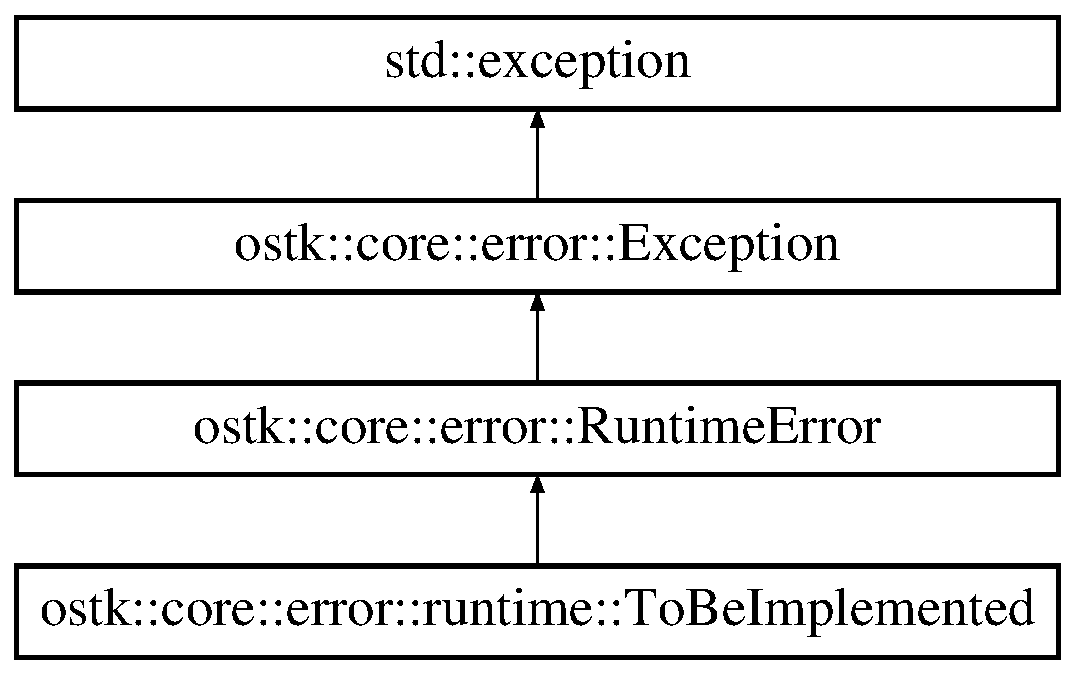
\includegraphics[height=4.000000cm]{classostk_1_1core_1_1error_1_1runtime_1_1_to_be_implemented}
\end{center}
\end{figure}
\subsection*{Public Member Functions}
\begin{DoxyCompactItemize}
\item 
\hyperlink{classostk_1_1core_1_1error_1_1runtime_1_1_to_be_implemented_a9bfd0da6b176670f0174794ef44c8420}{To\+Be\+Implemented} ()
\item 
\hyperlink{classostk_1_1core_1_1error_1_1runtime_1_1_to_be_implemented_aabda52249a2f3cbf4d17e1c877e8966c}{To\+Be\+Implemented} (const \hyperlink{classostk_1_1core_1_1types_1_1_string}{String} \&a\+Function\+Name)
\item 
\hyperlink{classostk_1_1core_1_1error_1_1runtime_1_1_to_be_implemented_a3383ca49c74c4969cda170c12ecff4a9}{$\sim$\+To\+Be\+Implemented} ()
\end{DoxyCompactItemize}


\subsection{Detailed Description}
To be implemented error class. 

\subsection{Constructor \& Destructor Documentation}
\mbox{\Hypertarget{classostk_1_1core_1_1error_1_1runtime_1_1_to_be_implemented_a9bfd0da6b176670f0174794ef44c8420}\label{classostk_1_1core_1_1error_1_1runtime_1_1_to_be_implemented_a9bfd0da6b176670f0174794ef44c8420}} 
\index{ostk\+::core\+::error\+::runtime\+::\+To\+Be\+Implemented@{ostk\+::core\+::error\+::runtime\+::\+To\+Be\+Implemented}!To\+Be\+Implemented@{To\+Be\+Implemented}}
\index{To\+Be\+Implemented@{To\+Be\+Implemented}!ostk\+::core\+::error\+::runtime\+::\+To\+Be\+Implemented@{ostk\+::core\+::error\+::runtime\+::\+To\+Be\+Implemented}}
\subsubsection{\texorpdfstring{To\+Be\+Implemented()}{ToBeImplemented()}\hspace{0.1cm}{\footnotesize\ttfamily [1/2]}}
{\footnotesize\ttfamily ostk\+::core\+::error\+::runtime\+::\+To\+Be\+Implemented\+::\+To\+Be\+Implemented (\begin{DoxyParamCaption}{ }\end{DoxyParamCaption})}

\mbox{\Hypertarget{classostk_1_1core_1_1error_1_1runtime_1_1_to_be_implemented_aabda52249a2f3cbf4d17e1c877e8966c}\label{classostk_1_1core_1_1error_1_1runtime_1_1_to_be_implemented_aabda52249a2f3cbf4d17e1c877e8966c}} 
\index{ostk\+::core\+::error\+::runtime\+::\+To\+Be\+Implemented@{ostk\+::core\+::error\+::runtime\+::\+To\+Be\+Implemented}!To\+Be\+Implemented@{To\+Be\+Implemented}}
\index{To\+Be\+Implemented@{To\+Be\+Implemented}!ostk\+::core\+::error\+::runtime\+::\+To\+Be\+Implemented@{ostk\+::core\+::error\+::runtime\+::\+To\+Be\+Implemented}}
\subsubsection{\texorpdfstring{To\+Be\+Implemented()}{ToBeImplemented()}\hspace{0.1cm}{\footnotesize\ttfamily [2/2]}}
{\footnotesize\ttfamily ostk\+::core\+::error\+::runtime\+::\+To\+Be\+Implemented\+::\+To\+Be\+Implemented (\begin{DoxyParamCaption}\item[{const \hyperlink{classostk_1_1core_1_1types_1_1_string}{String} \&}]{a\+Function\+Name }\end{DoxyParamCaption})}

\mbox{\Hypertarget{classostk_1_1core_1_1error_1_1runtime_1_1_to_be_implemented_a3383ca49c74c4969cda170c12ecff4a9}\label{classostk_1_1core_1_1error_1_1runtime_1_1_to_be_implemented_a3383ca49c74c4969cda170c12ecff4a9}} 
\index{ostk\+::core\+::error\+::runtime\+::\+To\+Be\+Implemented@{ostk\+::core\+::error\+::runtime\+::\+To\+Be\+Implemented}!````~To\+Be\+Implemented@{$\sim$\+To\+Be\+Implemented}}
\index{````~To\+Be\+Implemented@{$\sim$\+To\+Be\+Implemented}!ostk\+::core\+::error\+::runtime\+::\+To\+Be\+Implemented@{ostk\+::core\+::error\+::runtime\+::\+To\+Be\+Implemented}}
\subsubsection{\texorpdfstring{$\sim$\+To\+Be\+Implemented()}{~ToBeImplemented()}}
{\footnotesize\ttfamily ostk\+::core\+::error\+::runtime\+::\+To\+Be\+Implemented\+::$\sim$\+To\+Be\+Implemented (\begin{DoxyParamCaption}{ }\end{DoxyParamCaption})}



The documentation for this class was generated from the following files\+:\begin{DoxyCompactItemize}
\item 
include/\+Open\+Space\+Toolkit/\+Core/\+Error/\+Runtime/\hyperlink{_to_be_implemented_8hpp}{To\+Be\+Implemented.\+hpp}\item 
src/\+Open\+Space\+Toolkit/\+Core/\+Error/\+Runtime/\hyperlink{_to_be_implemented_8cpp}{To\+Be\+Implemented.\+cpp}\end{DoxyCompactItemize}

\hypertarget{classostk_1_1core_1_1ctnr_1_1_tree}{}\section{ostk\+:\+:core\+:\+:ctnr\+:\+:Tree Class Reference}
\label{classostk_1_1core_1_1ctnr_1_1_tree}\index{ostk\+::core\+::ctnr\+::\+Tree@{ostk\+::core\+::ctnr\+::\+Tree}}


Undirected graph in which any two vertices are connected by exactly one path.  




{\ttfamily \#include $<$Tree.\+hpp$>$}

\subsection*{Public Member Functions}
\begin{DoxyCompactItemize}
\item 
\hyperlink{classostk_1_1core_1_1ctnr_1_1_tree_a3960a2c77a482f88cdcdf5271b295815}{Tree} ()=delete
\item 
\hyperlink{classostk_1_1core_1_1ctnr_1_1_tree_a45d8c4d19771271433f1fcd525b9aaaf}{Tree} (const \hyperlink{classostk_1_1core_1_1ctnr_1_1_tree}{Tree} \&a\+Tree)
\item 
\hyperlink{classostk_1_1core_1_1ctnr_1_1_tree_a1fbbf116265bc413c82188dc8f406883}{$\sim$\+Tree} ()
\item 
\hyperlink{classostk_1_1core_1_1ctnr_1_1_tree}{Tree} \& \hyperlink{classostk_1_1core_1_1ctnr_1_1_tree_a9ef0c73b6fa96d246ae34b2131365fa1}{operator=} (const \hyperlink{classostk_1_1core_1_1ctnr_1_1_tree}{Tree} \&a\+Tree) const
\item 
bool \hyperlink{classostk_1_1core_1_1ctnr_1_1_tree_ac8fbfabe34924004a96cd5ad154bbfcc}{is\+Defined} () const
\end{DoxyCompactItemize}
\subsection*{Static Public Member Functions}
\begin{DoxyCompactItemize}
\item 
static \hyperlink{classostk_1_1core_1_1ctnr_1_1_tree}{Tree} \hyperlink{classostk_1_1core_1_1ctnr_1_1_tree_ace228911fa1c6f8e5a14d208ebb7717e}{Empty} ()
\item 
static \hyperlink{classostk_1_1core_1_1ctnr_1_1_tree}{Tree} \hyperlink{classostk_1_1core_1_1ctnr_1_1_tree_a958ec32a53858072b339952c7a69d8b7}{Object} (const \hyperlink{classostk_1_1core_1_1ctnr_1_1_object}{Object} \&an\+Object)
\end{DoxyCompactItemize}
\subsection*{Friends}
\begin{DoxyCompactItemize}
\item 
std\+::ostream \& \hyperlink{classostk_1_1core_1_1ctnr_1_1_tree_aca74cf66509d8f31b83b1c100cb00bea}{operator$<$$<$} (std\+::ostream \&an\+Output\+Stream, const \hyperlink{classostk_1_1core_1_1ctnr_1_1_tree}{Tree} \&a\+Tree)
\end{DoxyCompactItemize}


\subsection{Detailed Description}
Undirected graph in which any two vertices are connected by exactly one path. 

A tree data structure can be defined recursively (locally) as a collection of nodes (starting at a root node), where each node is a data structure consisting of a value, together with a list of references to nodes (the \char`\"{}children\char`\"{}), with the constraints that no reference is duplicated, and none points to the root.

https\+://en.wikipedia.\+org/wiki/\+Tree\+\_\+(graph\+\_\+theory) https\+://en.wikipedia.\+org/wiki/\+Tree\+\_\+(data\+\_\+structure) 

\subsection{Constructor \& Destructor Documentation}
\mbox{\Hypertarget{classostk_1_1core_1_1ctnr_1_1_tree_a3960a2c77a482f88cdcdf5271b295815}\label{classostk_1_1core_1_1ctnr_1_1_tree_a3960a2c77a482f88cdcdf5271b295815}} 
\index{ostk\+::core\+::ctnr\+::\+Tree@{ostk\+::core\+::ctnr\+::\+Tree}!Tree@{Tree}}
\index{Tree@{Tree}!ostk\+::core\+::ctnr\+::\+Tree@{ostk\+::core\+::ctnr\+::\+Tree}}
\subsubsection{\texorpdfstring{Tree()}{Tree()}\hspace{0.1cm}{\footnotesize\ttfamily [1/2]}}
{\footnotesize\ttfamily ostk\+::core\+::ctnr\+::\+Tree\+::\+Tree (\begin{DoxyParamCaption}{ }\end{DoxyParamCaption})\hspace{0.3cm}{\ttfamily [delete]}}

\mbox{\Hypertarget{classostk_1_1core_1_1ctnr_1_1_tree_a45d8c4d19771271433f1fcd525b9aaaf}\label{classostk_1_1core_1_1ctnr_1_1_tree_a45d8c4d19771271433f1fcd525b9aaaf}} 
\index{ostk\+::core\+::ctnr\+::\+Tree@{ostk\+::core\+::ctnr\+::\+Tree}!Tree@{Tree}}
\index{Tree@{Tree}!ostk\+::core\+::ctnr\+::\+Tree@{ostk\+::core\+::ctnr\+::\+Tree}}
\subsubsection{\texorpdfstring{Tree()}{Tree()}\hspace{0.1cm}{\footnotesize\ttfamily [2/2]}}
{\footnotesize\ttfamily ostk\+::core\+::ctnr\+::\+Tree\+::\+Tree (\begin{DoxyParamCaption}\item[{const \hyperlink{classostk_1_1core_1_1ctnr_1_1_tree}{Tree} \&}]{a\+Tree }\end{DoxyParamCaption})}

\mbox{\Hypertarget{classostk_1_1core_1_1ctnr_1_1_tree_a1fbbf116265bc413c82188dc8f406883}\label{classostk_1_1core_1_1ctnr_1_1_tree_a1fbbf116265bc413c82188dc8f406883}} 
\index{ostk\+::core\+::ctnr\+::\+Tree@{ostk\+::core\+::ctnr\+::\+Tree}!````~Tree@{$\sim$\+Tree}}
\index{````~Tree@{$\sim$\+Tree}!ostk\+::core\+::ctnr\+::\+Tree@{ostk\+::core\+::ctnr\+::\+Tree}}
\subsubsection{\texorpdfstring{$\sim$\+Tree()}{~Tree()}}
{\footnotesize\ttfamily ostk\+::core\+::ctnr\+::\+Tree\+::$\sim$\+Tree (\begin{DoxyParamCaption}{ }\end{DoxyParamCaption})}



\subsection{Member Function Documentation}
\mbox{\Hypertarget{classostk_1_1core_1_1ctnr_1_1_tree_ace228911fa1c6f8e5a14d208ebb7717e}\label{classostk_1_1core_1_1ctnr_1_1_tree_ace228911fa1c6f8e5a14d208ebb7717e}} 
\index{ostk\+::core\+::ctnr\+::\+Tree@{ostk\+::core\+::ctnr\+::\+Tree}!Empty@{Empty}}
\index{Empty@{Empty}!ostk\+::core\+::ctnr\+::\+Tree@{ostk\+::core\+::ctnr\+::\+Tree}}
\subsubsection{\texorpdfstring{Empty()}{Empty()}}
{\footnotesize\ttfamily static \hyperlink{classostk_1_1core_1_1ctnr_1_1_tree}{Tree} ostk\+::core\+::ctnr\+::\+Tree\+::\+Empty (\begin{DoxyParamCaption}{ }\end{DoxyParamCaption})\hspace{0.3cm}{\ttfamily [static]}}

\mbox{\Hypertarget{classostk_1_1core_1_1ctnr_1_1_tree_ac8fbfabe34924004a96cd5ad154bbfcc}\label{classostk_1_1core_1_1ctnr_1_1_tree_ac8fbfabe34924004a96cd5ad154bbfcc}} 
\index{ostk\+::core\+::ctnr\+::\+Tree@{ostk\+::core\+::ctnr\+::\+Tree}!is\+Defined@{is\+Defined}}
\index{is\+Defined@{is\+Defined}!ostk\+::core\+::ctnr\+::\+Tree@{ostk\+::core\+::ctnr\+::\+Tree}}
\subsubsection{\texorpdfstring{is\+Defined()}{isDefined()}}
{\footnotesize\ttfamily bool ostk\+::core\+::ctnr\+::\+Tree\+::is\+Defined (\begin{DoxyParamCaption}{ }\end{DoxyParamCaption}) const}

\mbox{\Hypertarget{classostk_1_1core_1_1ctnr_1_1_tree_a958ec32a53858072b339952c7a69d8b7}\label{classostk_1_1core_1_1ctnr_1_1_tree_a958ec32a53858072b339952c7a69d8b7}} 
\index{ostk\+::core\+::ctnr\+::\+Tree@{ostk\+::core\+::ctnr\+::\+Tree}!Object@{Object}}
\index{Object@{Object}!ostk\+::core\+::ctnr\+::\+Tree@{ostk\+::core\+::ctnr\+::\+Tree}}
\subsubsection{\texorpdfstring{Object()}{Object()}}
{\footnotesize\ttfamily static \hyperlink{classostk_1_1core_1_1ctnr_1_1_tree}{Tree} ostk\+::core\+::ctnr\+::\+Tree\+::\+Object (\begin{DoxyParamCaption}\item[{const \hyperlink{classostk_1_1core_1_1ctnr_1_1_object}{Object} \&}]{an\+Object }\end{DoxyParamCaption})\hspace{0.3cm}{\ttfamily [static]}}

\mbox{\Hypertarget{classostk_1_1core_1_1ctnr_1_1_tree_a9ef0c73b6fa96d246ae34b2131365fa1}\label{classostk_1_1core_1_1ctnr_1_1_tree_a9ef0c73b6fa96d246ae34b2131365fa1}} 
\index{ostk\+::core\+::ctnr\+::\+Tree@{ostk\+::core\+::ctnr\+::\+Tree}!operator=@{operator=}}
\index{operator=@{operator=}!ostk\+::core\+::ctnr\+::\+Tree@{ostk\+::core\+::ctnr\+::\+Tree}}
\subsubsection{\texorpdfstring{operator=()}{operator=()}}
{\footnotesize\ttfamily \hyperlink{classostk_1_1core_1_1ctnr_1_1_tree}{Tree}\& ostk\+::core\+::ctnr\+::\+Tree\+::operator= (\begin{DoxyParamCaption}\item[{const \hyperlink{classostk_1_1core_1_1ctnr_1_1_tree}{Tree} \&}]{a\+Tree }\end{DoxyParamCaption}) const}



\subsection{Friends And Related Function Documentation}
\mbox{\Hypertarget{classostk_1_1core_1_1ctnr_1_1_tree_aca74cf66509d8f31b83b1c100cb00bea}\label{classostk_1_1core_1_1ctnr_1_1_tree_aca74cf66509d8f31b83b1c100cb00bea}} 
\index{ostk\+::core\+::ctnr\+::\+Tree@{ostk\+::core\+::ctnr\+::\+Tree}!operator$<$$<$@{operator$<$$<$}}
\index{operator$<$$<$@{operator$<$$<$}!ostk\+::core\+::ctnr\+::\+Tree@{ostk\+::core\+::ctnr\+::\+Tree}}
\subsubsection{\texorpdfstring{operator$<$$<$}{operator<<}}
{\footnotesize\ttfamily std\+::ostream\& operator$<$$<$ (\begin{DoxyParamCaption}\item[{std\+::ostream \&}]{an\+Output\+Stream,  }\item[{const \hyperlink{classostk_1_1core_1_1ctnr_1_1_tree}{Tree} \&}]{a\+Tree }\end{DoxyParamCaption})\hspace{0.3cm}{\ttfamily [friend]}}



The documentation for this class was generated from the following file\+:\begin{DoxyCompactItemize}
\item 
include/\+Open\+Space\+Toolkit/\+Core/\+Containers/\hyperlink{_tree_8hpp}{Tree.\+hpp}\end{DoxyCompactItemize}

\hypertarget{structostk_1_1core_1_1ctnr_1_1_triple}{}\section{ostk\+:\+:core\+:\+:ctnr\+:\+:Triple$<$ T, U, V $>$ Struct Template Reference}
\label{structostk_1_1core_1_1ctnr_1_1_triple}\index{ostk\+::core\+::ctnr\+::\+Triple$<$ T, U, V $>$@{ostk\+::core\+::ctnr\+::\+Triple$<$ T, U, V $>$}}


\hyperlink{structostk_1_1core_1_1ctnr_1_1_triple}{Triple} container.  




{\ttfamily \#include $<$Triple.\+hpp$>$}

\subsection*{Public Attributes}
\begin{DoxyCompactItemize}
\item 
T \hyperlink{structostk_1_1core_1_1ctnr_1_1_triple_a0cc41738c17be0038d440821f2e8022a}{first}
\item 
U \hyperlink{structostk_1_1core_1_1ctnr_1_1_triple_a20851607908231eb1bca53693655a31c}{second}
\item 
V \hyperlink{structostk_1_1core_1_1ctnr_1_1_triple_a47c1a85baaeeff5ca5e08cf93047c2d2}{third}
\end{DoxyCompactItemize}


\subsection{Detailed Description}
\subsubsection*{template$<$typename T, typename U, typename V$>$\newline
struct ostk\+::core\+::ctnr\+::\+Triple$<$ T, U, V $>$}

\hyperlink{structostk_1_1core_1_1ctnr_1_1_triple}{Triple} container. 

\subsection{Member Data Documentation}
\mbox{\Hypertarget{structostk_1_1core_1_1ctnr_1_1_triple_a0cc41738c17be0038d440821f2e8022a}\label{structostk_1_1core_1_1ctnr_1_1_triple_a0cc41738c17be0038d440821f2e8022a}} 
\index{ostk\+::core\+::ctnr\+::\+Triple@{ostk\+::core\+::ctnr\+::\+Triple}!first@{first}}
\index{first@{first}!ostk\+::core\+::ctnr\+::\+Triple@{ostk\+::core\+::ctnr\+::\+Triple}}
\subsubsection{\texorpdfstring{first}{first}}
{\footnotesize\ttfamily template$<$typename T, typename U, typename V$>$ \\
T \hyperlink{structostk_1_1core_1_1ctnr_1_1_triple}{ostk\+::core\+::ctnr\+::\+Triple}$<$ T, U, V $>$\+::first}

\mbox{\Hypertarget{structostk_1_1core_1_1ctnr_1_1_triple_a20851607908231eb1bca53693655a31c}\label{structostk_1_1core_1_1ctnr_1_1_triple_a20851607908231eb1bca53693655a31c}} 
\index{ostk\+::core\+::ctnr\+::\+Triple@{ostk\+::core\+::ctnr\+::\+Triple}!second@{second}}
\index{second@{second}!ostk\+::core\+::ctnr\+::\+Triple@{ostk\+::core\+::ctnr\+::\+Triple}}
\subsubsection{\texorpdfstring{second}{second}}
{\footnotesize\ttfamily template$<$typename T, typename U, typename V$>$ \\
U \hyperlink{structostk_1_1core_1_1ctnr_1_1_triple}{ostk\+::core\+::ctnr\+::\+Triple}$<$ T, U, V $>$\+::second}

\mbox{\Hypertarget{structostk_1_1core_1_1ctnr_1_1_triple_a47c1a85baaeeff5ca5e08cf93047c2d2}\label{structostk_1_1core_1_1ctnr_1_1_triple_a47c1a85baaeeff5ca5e08cf93047c2d2}} 
\index{ostk\+::core\+::ctnr\+::\+Triple@{ostk\+::core\+::ctnr\+::\+Triple}!third@{third}}
\index{third@{third}!ostk\+::core\+::ctnr\+::\+Triple@{ostk\+::core\+::ctnr\+::\+Triple}}
\subsubsection{\texorpdfstring{third}{third}}
{\footnotesize\ttfamily template$<$typename T, typename U, typename V$>$ \\
V \hyperlink{structostk_1_1core_1_1ctnr_1_1_triple}{ostk\+::core\+::ctnr\+::\+Triple}$<$ T, U, V $>$\+::third}



The documentation for this struct was generated from the following file\+:\begin{DoxyCompactItemize}
\item 
include/\+Open\+Space\+Toolkit/\+Core/\+Containers/\hyperlink{_triple_8hpp}{Triple.\+hpp}\end{DoxyCompactItemize}

\hypertarget{classostk_1_1core_1_1error_1_1runtime_1_1_undefined}{}\section{ostk\+:\+:core\+:\+:error\+:\+:runtime\+:\+:Undefined Class Reference}
\label{classostk_1_1core_1_1error_1_1runtime_1_1_undefined}\index{ostk\+::core\+::error\+::runtime\+::\+Undefined@{ostk\+::core\+::error\+::runtime\+::\+Undefined}}


\hyperlink{classostk_1_1core_1_1error_1_1runtime_1_1_undefined}{Undefined} variable error class.  




{\ttfamily \#include $<$Undefined.\+hpp$>$}

Inheritance diagram for ostk\+:\+:core\+:\+:error\+:\+:runtime\+:\+:Undefined\+:\begin{figure}[H]
\begin{center}
\leavevmode
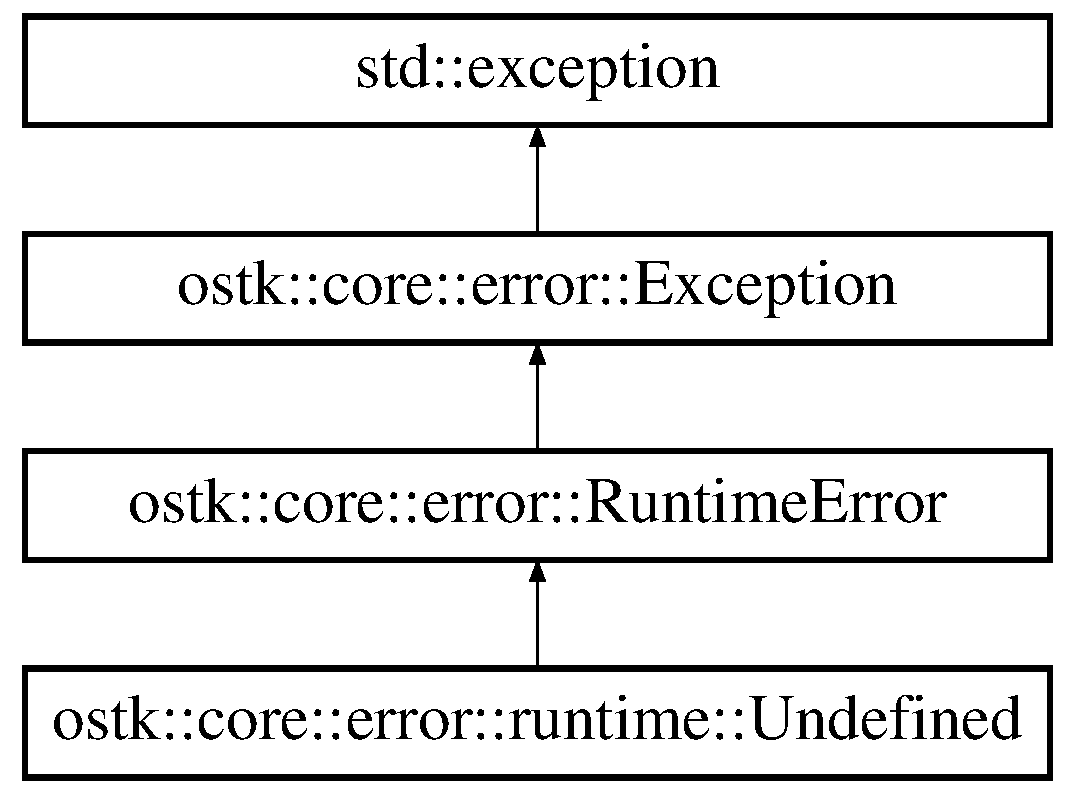
\includegraphics[height=4.000000cm]{classostk_1_1core_1_1error_1_1runtime_1_1_undefined}
\end{center}
\end{figure}
\subsection*{Public Member Functions}
\begin{DoxyCompactItemize}
\item 
\hyperlink{classostk_1_1core_1_1error_1_1runtime_1_1_undefined_a5ae214a1665596b08d53189168827a01}{Undefined} (const \hyperlink{classostk_1_1core_1_1types_1_1_string}{String} \&a\+Variable\+Name)
\item 
\hyperlink{classostk_1_1core_1_1error_1_1runtime_1_1_undefined_a0fd23d55bea868ae30b50f6d2690d6b9}{$\sim$\+Undefined} ()
\end{DoxyCompactItemize}


\subsection{Detailed Description}
\hyperlink{classostk_1_1core_1_1error_1_1runtime_1_1_undefined}{Undefined} variable error class. 

\subsection{Constructor \& Destructor Documentation}
\mbox{\Hypertarget{classostk_1_1core_1_1error_1_1runtime_1_1_undefined_a5ae214a1665596b08d53189168827a01}\label{classostk_1_1core_1_1error_1_1runtime_1_1_undefined_a5ae214a1665596b08d53189168827a01}} 
\index{ostk\+::core\+::error\+::runtime\+::\+Undefined@{ostk\+::core\+::error\+::runtime\+::\+Undefined}!Undefined@{Undefined}}
\index{Undefined@{Undefined}!ostk\+::core\+::error\+::runtime\+::\+Undefined@{ostk\+::core\+::error\+::runtime\+::\+Undefined}}
\subsubsection{\texorpdfstring{Undefined()}{Undefined()}}
{\footnotesize\ttfamily ostk\+::core\+::error\+::runtime\+::\+Undefined\+::\+Undefined (\begin{DoxyParamCaption}\item[{const \hyperlink{classostk_1_1core_1_1types_1_1_string}{String} \&}]{a\+Variable\+Name }\end{DoxyParamCaption})}

\mbox{\Hypertarget{classostk_1_1core_1_1error_1_1runtime_1_1_undefined_a0fd23d55bea868ae30b50f6d2690d6b9}\label{classostk_1_1core_1_1error_1_1runtime_1_1_undefined_a0fd23d55bea868ae30b50f6d2690d6b9}} 
\index{ostk\+::core\+::error\+::runtime\+::\+Undefined@{ostk\+::core\+::error\+::runtime\+::\+Undefined}!````~Undefined@{$\sim$\+Undefined}}
\index{````~Undefined@{$\sim$\+Undefined}!ostk\+::core\+::error\+::runtime\+::\+Undefined@{ostk\+::core\+::error\+::runtime\+::\+Undefined}}
\subsubsection{\texorpdfstring{$\sim$\+Undefined()}{~Undefined()}}
{\footnotesize\ttfamily ostk\+::core\+::error\+::runtime\+::\+Undefined\+::$\sim$\+Undefined (\begin{DoxyParamCaption}{ }\end{DoxyParamCaption})}



The documentation for this class was generated from the following files\+:\begin{DoxyCompactItemize}
\item 
include/\+Open\+Space\+Toolkit/\+Core/\+Error/\+Runtime/\hyperlink{_undefined_8hpp}{Undefined.\+hpp}\item 
src/\+Open\+Space\+Toolkit/\+Core/\+Error/\+Runtime/\hyperlink{_undefined_8cpp}{Undefined.\+cpp}\end{DoxyCompactItemize}

\hypertarget{classostk_1_1core_1_1system_1_1_user}{}\section{ostk\+:\+:core\+:\+:system\+:\+:User Class Reference}
\label{classostk_1_1core_1_1system_1_1_user}\index{ostk\+::core\+::system\+::\+User@{ostk\+::core\+::system\+::\+User}}


\hyperlink{classostk_1_1core_1_1system_1_1_user}{User}.  




{\ttfamily \#include $<$User.\+hpp$>$}

\subsection*{Public Member Functions}
\begin{DoxyCompactItemize}
\item 
\hyperlink{classostk_1_1core_1_1system_1_1_user_a0de9691c8ea414402a61ca2ba571125b}{User} (const uint \&a\+U\+ID, const \hyperlink{classostk_1_1core_1_1types_1_1_string}{String} \&a\+Name)
\item 
\hyperlink{classostk_1_1core_1_1system_1_1_user_a136687a5b8b44617158bb3d14d4697c8}{User} (const uint \&a\+U\+ID, const uint \&a\+E\+U\+ID, const \hyperlink{classostk_1_1core_1_1types_1_1_string}{String} \&a\+Name)
\item 
bool \hyperlink{classostk_1_1core_1_1system_1_1_user_a58e11432b4f5e0c37edf841d3360f58b}{operator==} (const \hyperlink{classostk_1_1core_1_1system_1_1_user}{User} \&a\+User) const
\item 
bool \hyperlink{classostk_1_1core_1_1system_1_1_user_ac11fea5211b9e8faa2ae07c1ba5fa154}{operator!=} (const \hyperlink{classostk_1_1core_1_1system_1_1_user}{User} \&a\+User) const
\item 
bool \hyperlink{classostk_1_1core_1_1system_1_1_user_a8db1aaed91e6eca5459230cd28931e56}{is\+Defined} () const
\item 
int \hyperlink{classostk_1_1core_1_1system_1_1_user_acc8330f48805da8a188c0b38ef815a03}{get\+U\+ID} () const
\item 
int \hyperlink{classostk_1_1core_1_1system_1_1_user_ac4c9c03e93d714ccf43b6160c73e9604}{get\+E\+U\+ID} () const
\item 
\hyperlink{classostk_1_1core_1_1types_1_1_string}{String} \hyperlink{classostk_1_1core_1_1system_1_1_user_a1f112f97f90b2910c943d22aff6f66f5}{get\+Name} () const
\end{DoxyCompactItemize}
\subsection*{Static Public Member Functions}
\begin{DoxyCompactItemize}
\item 
static \hyperlink{classostk_1_1core_1_1system_1_1_user}{User} \hyperlink{classostk_1_1core_1_1system_1_1_user_ad5a31224086dca11b4795adbddd82759}{Undefined} ()
\item 
static \hyperlink{classostk_1_1core_1_1system_1_1_user}{User} \hyperlink{classostk_1_1core_1_1system_1_1_user_adc854960802510e2dcc4c45bbb1ab0a5}{Process} ()
\item 
static \hyperlink{classostk_1_1core_1_1system_1_1_user}{User} \hyperlink{classostk_1_1core_1_1system_1_1_user_a7625cdddf50a15320fca6d18e67ae848}{U\+ID} (const uint \&a\+U\+ID)
\item 
static \hyperlink{classostk_1_1core_1_1system_1_1_user}{User} \hyperlink{classostk_1_1core_1_1system_1_1_user_a83abc0dd6771386923d28c2106e107b7}{Name} (const \hyperlink{classostk_1_1core_1_1types_1_1_string}{String} \&a\+Name)
\end{DoxyCompactItemize}
\subsection*{Friends}
\begin{DoxyCompactItemize}
\item 
std\+::ostream \& \hyperlink{classostk_1_1core_1_1system_1_1_user_ac434498b36c6e29a86acbb50589e91a3}{operator$<$$<$} (std\+::ostream \&an\+Output\+Stream, const \hyperlink{classostk_1_1core_1_1system_1_1_user}{User} \&a\+User)
\end{DoxyCompactItemize}


\subsection{Detailed Description}
\hyperlink{classostk_1_1core_1_1system_1_1_user}{User}. 

P\+O\+S\+IX compliant

https\+://en.wikipedia.\+org/wiki/\+User\+\_\+identifier 

\subsection{Constructor \& Destructor Documentation}
\mbox{\Hypertarget{classostk_1_1core_1_1system_1_1_user_a0de9691c8ea414402a61ca2ba571125b}\label{classostk_1_1core_1_1system_1_1_user_a0de9691c8ea414402a61ca2ba571125b}} 
\index{ostk\+::core\+::system\+::\+User@{ostk\+::core\+::system\+::\+User}!User@{User}}
\index{User@{User}!ostk\+::core\+::system\+::\+User@{ostk\+::core\+::system\+::\+User}}
\subsubsection{\texorpdfstring{User()}{User()}\hspace{0.1cm}{\footnotesize\ttfamily [1/2]}}
{\footnotesize\ttfamily ostk\+::core\+::system\+::\+User\+::\+User (\begin{DoxyParamCaption}\item[{const uint \&}]{a\+U\+ID,  }\item[{const \hyperlink{classostk_1_1core_1_1types_1_1_string}{String} \&}]{a\+Name }\end{DoxyParamCaption})}

\mbox{\Hypertarget{classostk_1_1core_1_1system_1_1_user_a136687a5b8b44617158bb3d14d4697c8}\label{classostk_1_1core_1_1system_1_1_user_a136687a5b8b44617158bb3d14d4697c8}} 
\index{ostk\+::core\+::system\+::\+User@{ostk\+::core\+::system\+::\+User}!User@{User}}
\index{User@{User}!ostk\+::core\+::system\+::\+User@{ostk\+::core\+::system\+::\+User}}
\subsubsection{\texorpdfstring{User()}{User()}\hspace{0.1cm}{\footnotesize\ttfamily [2/2]}}
{\footnotesize\ttfamily ostk\+::core\+::system\+::\+User\+::\+User (\begin{DoxyParamCaption}\item[{const uint \&}]{a\+U\+ID,  }\item[{const uint \&}]{a\+E\+U\+ID,  }\item[{const \hyperlink{classostk_1_1core_1_1types_1_1_string}{String} \&}]{a\+Name }\end{DoxyParamCaption})}



\subsection{Member Function Documentation}
\mbox{\Hypertarget{classostk_1_1core_1_1system_1_1_user_ac4c9c03e93d714ccf43b6160c73e9604}\label{classostk_1_1core_1_1system_1_1_user_ac4c9c03e93d714ccf43b6160c73e9604}} 
\index{ostk\+::core\+::system\+::\+User@{ostk\+::core\+::system\+::\+User}!get\+E\+U\+ID@{get\+E\+U\+ID}}
\index{get\+E\+U\+ID@{get\+E\+U\+ID}!ostk\+::core\+::system\+::\+User@{ostk\+::core\+::system\+::\+User}}
\subsubsection{\texorpdfstring{get\+E\+U\+I\+D()}{getEUID()}}
{\footnotesize\ttfamily int ostk\+::core\+::system\+::\+User\+::get\+E\+U\+ID (\begin{DoxyParamCaption}{ }\end{DoxyParamCaption}) const}

\mbox{\Hypertarget{classostk_1_1core_1_1system_1_1_user_a1f112f97f90b2910c943d22aff6f66f5}\label{classostk_1_1core_1_1system_1_1_user_a1f112f97f90b2910c943d22aff6f66f5}} 
\index{ostk\+::core\+::system\+::\+User@{ostk\+::core\+::system\+::\+User}!get\+Name@{get\+Name}}
\index{get\+Name@{get\+Name}!ostk\+::core\+::system\+::\+User@{ostk\+::core\+::system\+::\+User}}
\subsubsection{\texorpdfstring{get\+Name()}{getName()}}
{\footnotesize\ttfamily \hyperlink{classostk_1_1core_1_1types_1_1_string}{String} ostk\+::core\+::system\+::\+User\+::get\+Name (\begin{DoxyParamCaption}{ }\end{DoxyParamCaption}) const}

\mbox{\Hypertarget{classostk_1_1core_1_1system_1_1_user_acc8330f48805da8a188c0b38ef815a03}\label{classostk_1_1core_1_1system_1_1_user_acc8330f48805da8a188c0b38ef815a03}} 
\index{ostk\+::core\+::system\+::\+User@{ostk\+::core\+::system\+::\+User}!get\+U\+ID@{get\+U\+ID}}
\index{get\+U\+ID@{get\+U\+ID}!ostk\+::core\+::system\+::\+User@{ostk\+::core\+::system\+::\+User}}
\subsubsection{\texorpdfstring{get\+U\+I\+D()}{getUID()}}
{\footnotesize\ttfamily int ostk\+::core\+::system\+::\+User\+::get\+U\+ID (\begin{DoxyParamCaption}{ }\end{DoxyParamCaption}) const}

\mbox{\Hypertarget{classostk_1_1core_1_1system_1_1_user_a8db1aaed91e6eca5459230cd28931e56}\label{classostk_1_1core_1_1system_1_1_user_a8db1aaed91e6eca5459230cd28931e56}} 
\index{ostk\+::core\+::system\+::\+User@{ostk\+::core\+::system\+::\+User}!is\+Defined@{is\+Defined}}
\index{is\+Defined@{is\+Defined}!ostk\+::core\+::system\+::\+User@{ostk\+::core\+::system\+::\+User}}
\subsubsection{\texorpdfstring{is\+Defined()}{isDefined()}}
{\footnotesize\ttfamily bool ostk\+::core\+::system\+::\+User\+::is\+Defined (\begin{DoxyParamCaption}{ }\end{DoxyParamCaption}) const}

\mbox{\Hypertarget{classostk_1_1core_1_1system_1_1_user_a83abc0dd6771386923d28c2106e107b7}\label{classostk_1_1core_1_1system_1_1_user_a83abc0dd6771386923d28c2106e107b7}} 
\index{ostk\+::core\+::system\+::\+User@{ostk\+::core\+::system\+::\+User}!Name@{Name}}
\index{Name@{Name}!ostk\+::core\+::system\+::\+User@{ostk\+::core\+::system\+::\+User}}
\subsubsection{\texorpdfstring{Name()}{Name()}}
{\footnotesize\ttfamily static \hyperlink{classostk_1_1core_1_1system_1_1_user}{User} ostk\+::core\+::system\+::\+User\+::\+Name (\begin{DoxyParamCaption}\item[{const \hyperlink{classostk_1_1core_1_1types_1_1_string}{String} \&}]{a\+Name }\end{DoxyParamCaption})\hspace{0.3cm}{\ttfamily [static]}}

\mbox{\Hypertarget{classostk_1_1core_1_1system_1_1_user_ac11fea5211b9e8faa2ae07c1ba5fa154}\label{classostk_1_1core_1_1system_1_1_user_ac11fea5211b9e8faa2ae07c1ba5fa154}} 
\index{ostk\+::core\+::system\+::\+User@{ostk\+::core\+::system\+::\+User}!operator"!=@{operator"!=}}
\index{operator"!=@{operator"!=}!ostk\+::core\+::system\+::\+User@{ostk\+::core\+::system\+::\+User}}
\subsubsection{\texorpdfstring{operator"!=()}{operator!=()}}
{\footnotesize\ttfamily bool ostk\+::core\+::system\+::\+User\+::operator!= (\begin{DoxyParamCaption}\item[{const \hyperlink{classostk_1_1core_1_1system_1_1_user}{User} \&}]{a\+User }\end{DoxyParamCaption}) const}

\mbox{\Hypertarget{classostk_1_1core_1_1system_1_1_user_a58e11432b4f5e0c37edf841d3360f58b}\label{classostk_1_1core_1_1system_1_1_user_a58e11432b4f5e0c37edf841d3360f58b}} 
\index{ostk\+::core\+::system\+::\+User@{ostk\+::core\+::system\+::\+User}!operator==@{operator==}}
\index{operator==@{operator==}!ostk\+::core\+::system\+::\+User@{ostk\+::core\+::system\+::\+User}}
\subsubsection{\texorpdfstring{operator==()}{operator==()}}
{\footnotesize\ttfamily bool ostk\+::core\+::system\+::\+User\+::operator== (\begin{DoxyParamCaption}\item[{const \hyperlink{classostk_1_1core_1_1system_1_1_user}{User} \&}]{a\+User }\end{DoxyParamCaption}) const}

\mbox{\Hypertarget{classostk_1_1core_1_1system_1_1_user_adc854960802510e2dcc4c45bbb1ab0a5}\label{classostk_1_1core_1_1system_1_1_user_adc854960802510e2dcc4c45bbb1ab0a5}} 
\index{ostk\+::core\+::system\+::\+User@{ostk\+::core\+::system\+::\+User}!Process@{Process}}
\index{Process@{Process}!ostk\+::core\+::system\+::\+User@{ostk\+::core\+::system\+::\+User}}
\subsubsection{\texorpdfstring{Process()}{Process()}}
{\footnotesize\ttfamily static \hyperlink{classostk_1_1core_1_1system_1_1_user}{User} ostk\+::core\+::system\+::\+User\+::\+Process (\begin{DoxyParamCaption}{ }\end{DoxyParamCaption})\hspace{0.3cm}{\ttfamily [static]}}

\mbox{\Hypertarget{classostk_1_1core_1_1system_1_1_user_a7625cdddf50a15320fca6d18e67ae848}\label{classostk_1_1core_1_1system_1_1_user_a7625cdddf50a15320fca6d18e67ae848}} 
\index{ostk\+::core\+::system\+::\+User@{ostk\+::core\+::system\+::\+User}!U\+ID@{U\+ID}}
\index{U\+ID@{U\+ID}!ostk\+::core\+::system\+::\+User@{ostk\+::core\+::system\+::\+User}}
\subsubsection{\texorpdfstring{U\+I\+D()}{UID()}}
{\footnotesize\ttfamily static \hyperlink{classostk_1_1core_1_1system_1_1_user}{User} ostk\+::core\+::system\+::\+User\+::\+U\+ID (\begin{DoxyParamCaption}\item[{const uint \&}]{a\+U\+ID }\end{DoxyParamCaption})\hspace{0.3cm}{\ttfamily [static]}}

\mbox{\Hypertarget{classostk_1_1core_1_1system_1_1_user_ad5a31224086dca11b4795adbddd82759}\label{classostk_1_1core_1_1system_1_1_user_ad5a31224086dca11b4795adbddd82759}} 
\index{ostk\+::core\+::system\+::\+User@{ostk\+::core\+::system\+::\+User}!Undefined@{Undefined}}
\index{Undefined@{Undefined}!ostk\+::core\+::system\+::\+User@{ostk\+::core\+::system\+::\+User}}
\subsubsection{\texorpdfstring{Undefined()}{Undefined()}}
{\footnotesize\ttfamily static \hyperlink{classostk_1_1core_1_1system_1_1_user}{User} ostk\+::core\+::system\+::\+User\+::\+Undefined (\begin{DoxyParamCaption}{ }\end{DoxyParamCaption})\hspace{0.3cm}{\ttfamily [static]}}



\subsection{Friends And Related Function Documentation}
\mbox{\Hypertarget{classostk_1_1core_1_1system_1_1_user_ac434498b36c6e29a86acbb50589e91a3}\label{classostk_1_1core_1_1system_1_1_user_ac434498b36c6e29a86acbb50589e91a3}} 
\index{ostk\+::core\+::system\+::\+User@{ostk\+::core\+::system\+::\+User}!operator$<$$<$@{operator$<$$<$}}
\index{operator$<$$<$@{operator$<$$<$}!ostk\+::core\+::system\+::\+User@{ostk\+::core\+::system\+::\+User}}
\subsubsection{\texorpdfstring{operator$<$$<$}{operator<<}}
{\footnotesize\ttfamily std\+::ostream\& operator$<$$<$ (\begin{DoxyParamCaption}\item[{std\+::ostream \&}]{an\+Output\+Stream,  }\item[{const \hyperlink{classostk_1_1core_1_1system_1_1_user}{User} \&}]{a\+User }\end{DoxyParamCaption})\hspace{0.3cm}{\ttfamily [friend]}}



The documentation for this class was generated from the following file\+:\begin{DoxyCompactItemize}
\item 
include/\+Open\+Space\+Toolkit/\+Core/\+System/\hyperlink{_user_8hpp}{User.\+hpp}\end{DoxyCompactItemize}

\hypertarget{classostk_1_1core_1_1error_1_1runtime_1_1_wrong}{}\section{ostk\+:\+:core\+:\+:error\+:\+:runtime\+:\+:Wrong Class Reference}
\label{classostk_1_1core_1_1error_1_1runtime_1_1_wrong}\index{ostk\+::core\+::error\+::runtime\+::\+Wrong@{ostk\+::core\+::error\+::runtime\+::\+Wrong}}


\hyperlink{classostk_1_1core_1_1error_1_1runtime_1_1_wrong}{Wrong} variable error class.  




{\ttfamily \#include $<$Wrong.\+hpp$>$}

Inheritance diagram for ostk\+:\+:core\+:\+:error\+:\+:runtime\+:\+:Wrong\+:\begin{figure}[H]
\begin{center}
\leavevmode
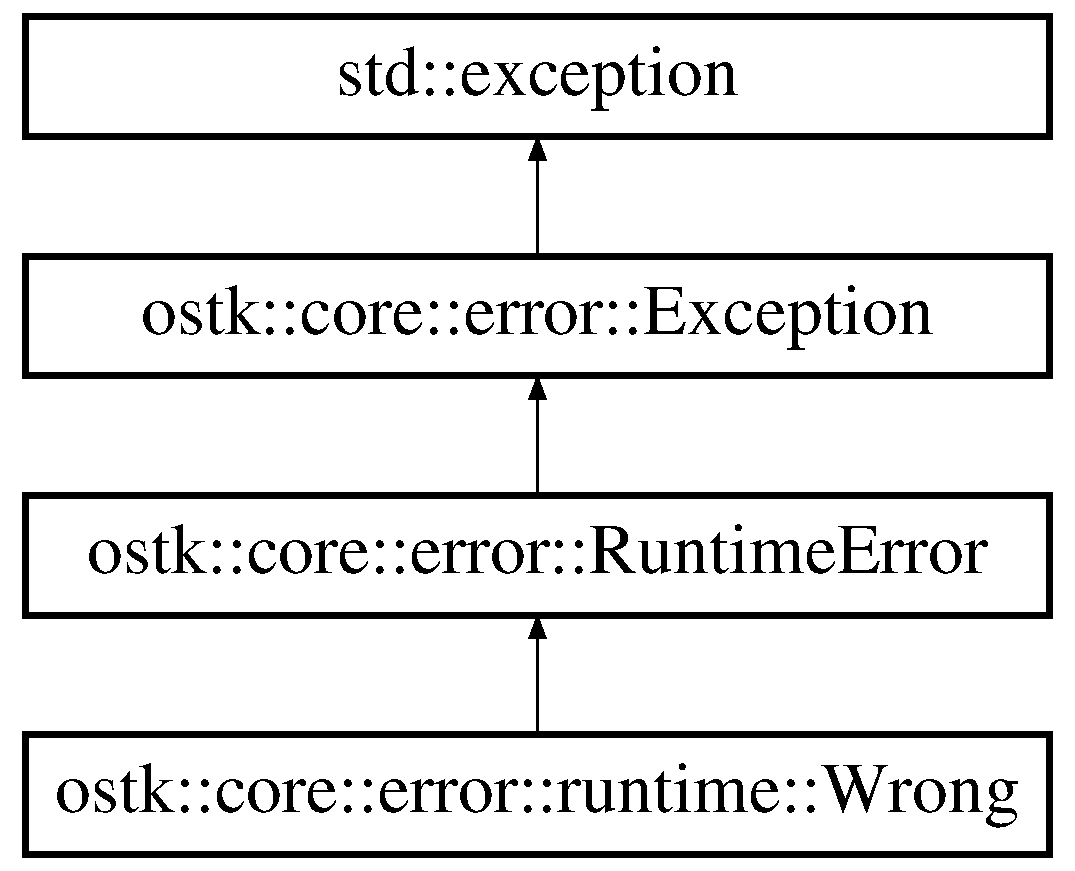
\includegraphics[height=4.000000cm]{classostk_1_1core_1_1error_1_1runtime_1_1_wrong}
\end{center}
\end{figure}
\subsection*{Public Member Functions}
\begin{DoxyCompactItemize}
\item 
\hyperlink{classostk_1_1core_1_1error_1_1runtime_1_1_wrong_a2e065c6ffb3877dd93fc36e897a54137}{Wrong} (const \hyperlink{classostk_1_1core_1_1types_1_1_string}{String} \&a\+Variable\+Name)
\item 
{\footnotesize template$<$typename ... Args$>$ }\\\hyperlink{classostk_1_1core_1_1error_1_1runtime_1_1_wrong_ac517c931c12598eed5d6b06272cfa303}{Wrong} (const \hyperlink{classostk_1_1core_1_1types_1_1_string}{String} \&a\+Variable\+Name, Args... an\+Argument\+List)
\item 
\hyperlink{classostk_1_1core_1_1error_1_1runtime_1_1_wrong_abc368bd88382a208840fd799fd7dc93b}{$\sim$\+Wrong} ()
\end{DoxyCompactItemize}


\subsection{Detailed Description}
\hyperlink{classostk_1_1core_1_1error_1_1runtime_1_1_wrong}{Wrong} variable error class. 

\subsection{Constructor \& Destructor Documentation}
\mbox{\Hypertarget{classostk_1_1core_1_1error_1_1runtime_1_1_wrong_a2e065c6ffb3877dd93fc36e897a54137}\label{classostk_1_1core_1_1error_1_1runtime_1_1_wrong_a2e065c6ffb3877dd93fc36e897a54137}} 
\index{ostk\+::core\+::error\+::runtime\+::\+Wrong@{ostk\+::core\+::error\+::runtime\+::\+Wrong}!Wrong@{Wrong}}
\index{Wrong@{Wrong}!ostk\+::core\+::error\+::runtime\+::\+Wrong@{ostk\+::core\+::error\+::runtime\+::\+Wrong}}
\subsubsection{\texorpdfstring{Wrong()}{Wrong()}\hspace{0.1cm}{\footnotesize\ttfamily [1/2]}}
{\footnotesize\ttfamily ostk\+::core\+::error\+::runtime\+::\+Wrong\+::\+Wrong (\begin{DoxyParamCaption}\item[{const \hyperlink{classostk_1_1core_1_1types_1_1_string}{String} \&}]{a\+Variable\+Name }\end{DoxyParamCaption})}

\mbox{\Hypertarget{classostk_1_1core_1_1error_1_1runtime_1_1_wrong_ac517c931c12598eed5d6b06272cfa303}\label{classostk_1_1core_1_1error_1_1runtime_1_1_wrong_ac517c931c12598eed5d6b06272cfa303}} 
\index{ostk\+::core\+::error\+::runtime\+::\+Wrong@{ostk\+::core\+::error\+::runtime\+::\+Wrong}!Wrong@{Wrong}}
\index{Wrong@{Wrong}!ostk\+::core\+::error\+::runtime\+::\+Wrong@{ostk\+::core\+::error\+::runtime\+::\+Wrong}}
\subsubsection{\texorpdfstring{Wrong()}{Wrong()}\hspace{0.1cm}{\footnotesize\ttfamily [2/2]}}
{\footnotesize\ttfamily template$<$typename ... Args$>$ \\
ostk\+::core\+::error\+::runtime\+::\+Wrong\+::\+Wrong (\begin{DoxyParamCaption}\item[{const \hyperlink{classostk_1_1core_1_1types_1_1_string}{String} \&}]{a\+Variable\+Name,  }\item[{Args...}]{an\+Argument\+List }\end{DoxyParamCaption})\hspace{0.3cm}{\ttfamily [inline]}}

\mbox{\Hypertarget{classostk_1_1core_1_1error_1_1runtime_1_1_wrong_abc368bd88382a208840fd799fd7dc93b}\label{classostk_1_1core_1_1error_1_1runtime_1_1_wrong_abc368bd88382a208840fd799fd7dc93b}} 
\index{ostk\+::core\+::error\+::runtime\+::\+Wrong@{ostk\+::core\+::error\+::runtime\+::\+Wrong}!````~Wrong@{$\sim$\+Wrong}}
\index{````~Wrong@{$\sim$\+Wrong}!ostk\+::core\+::error\+::runtime\+::\+Wrong@{ostk\+::core\+::error\+::runtime\+::\+Wrong}}
\subsubsection{\texorpdfstring{$\sim$\+Wrong()}{~Wrong()}}
{\footnotesize\ttfamily ostk\+::core\+::error\+::runtime\+::\+Wrong\+::$\sim$\+Wrong (\begin{DoxyParamCaption}{ }\end{DoxyParamCaption})}



The documentation for this class was generated from the following files\+:\begin{DoxyCompactItemize}
\item 
include/\+Open\+Space\+Toolkit/\+Core/\+Error/\+Runtime/\hyperlink{_wrong_8hpp}{Wrong.\+hpp}\item 
src/\+Open\+Space\+Toolkit/\+Core/\+Error/\+Runtime/\hyperlink{_wrong_8cpp}{Wrong.\+cpp}\end{DoxyCompactItemize}

\hypertarget{classostk_1_1core_1_1ctnr_1_1iterators_1_1_zip_iterator}{}\section{ostk\+:\+:core\+:\+:ctnr\+:\+:iterators\+:\+:Zip\+Iterator$<$ T $>$ Class Template Reference}
\label{classostk_1_1core_1_1ctnr_1_1iterators_1_1_zip_iterator}\index{ostk\+::core\+::ctnr\+::iterators\+::\+Zip\+Iterator$<$ T $>$@{ostk\+::core\+::ctnr\+::iterators\+::\+Zip\+Iterator$<$ T $>$}}


Zip iterator.  




{\ttfamily \#include $<$Zip.\+hpp$>$}

\subsection*{Classes}
\begin{DoxyCompactItemize}
\item 
class \hyperlink{classostk_1_1core_1_1ctnr_1_1iterators_1_1_zip_iterator_1_1_iterator}{Iterator}
\end{DoxyCompactItemize}
\subsection*{Public Member Functions}
\begin{DoxyCompactItemize}
\item 
\hyperlink{classostk_1_1core_1_1ctnr_1_1iterators_1_1_zip_iterator_ac3ac6cb006cd9428ea66235a9d240221}{Zip\+Iterator} (T \&... a\+Sequence)
\item 
\hyperlink{classostk_1_1core_1_1ctnr_1_1iterators_1_1_zip_iterator_1_1_iterator}{Zip\+Iterator\+::\+Iterator} \hyperlink{classostk_1_1core_1_1ctnr_1_1iterators_1_1_zip_iterator_a9fd76a0b2306f00757c5a09accef725a}{begin} () const
\item 
\hyperlink{classostk_1_1core_1_1ctnr_1_1iterators_1_1_zip_iterator_1_1_iterator}{Zip\+Iterator\+::\+Iterator} \hyperlink{classostk_1_1core_1_1ctnr_1_1iterators_1_1_zip_iterator_a470a84ee17b1e6ac0a92602cb97fca1a}{end} () const
\end{DoxyCompactItemize}


\subsection{Detailed Description}
\subsubsection*{template$<$typename... T$>$\newline
class ostk\+::core\+::ctnr\+::iterators\+::\+Zip\+Iterator$<$ T $>$}

Zip iterator. 

https\+://gist.github.\+com/mortehu/373069390c75b02f98b655e3f7dbef9a 

\subsection{Constructor \& Destructor Documentation}
\mbox{\Hypertarget{classostk_1_1core_1_1ctnr_1_1iterators_1_1_zip_iterator_ac3ac6cb006cd9428ea66235a9d240221}\label{classostk_1_1core_1_1ctnr_1_1iterators_1_1_zip_iterator_ac3ac6cb006cd9428ea66235a9d240221}} 
\index{ostk\+::core\+::ctnr\+::iterators\+::\+Zip\+Iterator@{ostk\+::core\+::ctnr\+::iterators\+::\+Zip\+Iterator}!Zip\+Iterator@{Zip\+Iterator}}
\index{Zip\+Iterator@{Zip\+Iterator}!ostk\+::core\+::ctnr\+::iterators\+::\+Zip\+Iterator@{ostk\+::core\+::ctnr\+::iterators\+::\+Zip\+Iterator}}
\subsubsection{\texorpdfstring{Zip\+Iterator()}{ZipIterator()}}
{\footnotesize\ttfamily template$<$typename... T$>$ \\
\hyperlink{classostk_1_1core_1_1ctnr_1_1iterators_1_1_zip_iterator}{ostk\+::core\+::ctnr\+::iterators\+::\+Zip\+Iterator}$<$ T $>$\+::\hyperlink{classostk_1_1core_1_1ctnr_1_1iterators_1_1_zip_iterator}{Zip\+Iterator} (\begin{DoxyParamCaption}\item[{T \&...}]{a\+Sequence }\end{DoxyParamCaption})\hspace{0.3cm}{\ttfamily [inline]}}



\subsection{Member Function Documentation}
\mbox{\Hypertarget{classostk_1_1core_1_1ctnr_1_1iterators_1_1_zip_iterator_a9fd76a0b2306f00757c5a09accef725a}\label{classostk_1_1core_1_1ctnr_1_1iterators_1_1_zip_iterator_a9fd76a0b2306f00757c5a09accef725a}} 
\index{ostk\+::core\+::ctnr\+::iterators\+::\+Zip\+Iterator@{ostk\+::core\+::ctnr\+::iterators\+::\+Zip\+Iterator}!begin@{begin}}
\index{begin@{begin}!ostk\+::core\+::ctnr\+::iterators\+::\+Zip\+Iterator@{ostk\+::core\+::ctnr\+::iterators\+::\+Zip\+Iterator}}
\subsubsection{\texorpdfstring{begin()}{begin()}}
{\footnotesize\ttfamily template$<$typename... T$>$ \\
\hyperlink{classostk_1_1core_1_1ctnr_1_1iterators_1_1_zip_iterator_1_1_iterator}{Zip\+Iterator\+::\+Iterator} \hyperlink{classostk_1_1core_1_1ctnr_1_1iterators_1_1_zip_iterator}{ostk\+::core\+::ctnr\+::iterators\+::\+Zip\+Iterator}$<$ T $>$\+::begin (\begin{DoxyParamCaption}{ }\end{DoxyParamCaption}) const\hspace{0.3cm}{\ttfamily [inline]}}

\mbox{\Hypertarget{classostk_1_1core_1_1ctnr_1_1iterators_1_1_zip_iterator_a470a84ee17b1e6ac0a92602cb97fca1a}\label{classostk_1_1core_1_1ctnr_1_1iterators_1_1_zip_iterator_a470a84ee17b1e6ac0a92602cb97fca1a}} 
\index{ostk\+::core\+::ctnr\+::iterators\+::\+Zip\+Iterator@{ostk\+::core\+::ctnr\+::iterators\+::\+Zip\+Iterator}!end@{end}}
\index{end@{end}!ostk\+::core\+::ctnr\+::iterators\+::\+Zip\+Iterator@{ostk\+::core\+::ctnr\+::iterators\+::\+Zip\+Iterator}}
\subsubsection{\texorpdfstring{end()}{end()}}
{\footnotesize\ttfamily template$<$typename... T$>$ \\
\hyperlink{classostk_1_1core_1_1ctnr_1_1iterators_1_1_zip_iterator_1_1_iterator}{Zip\+Iterator\+::\+Iterator} \hyperlink{classostk_1_1core_1_1ctnr_1_1iterators_1_1_zip_iterator}{ostk\+::core\+::ctnr\+::iterators\+::\+Zip\+Iterator}$<$ T $>$\+::end (\begin{DoxyParamCaption}{ }\end{DoxyParamCaption}) const\hspace{0.3cm}{\ttfamily [inline]}}



The documentation for this class was generated from the following file\+:\begin{DoxyCompactItemize}
\item 
include/\+Open\+Space\+Toolkit/\+Core/\+Containers/\+Iterators/\hyperlink{_zip_8hpp}{Zip.\+hpp}\end{DoxyCompactItemize}

\chapter{File Documentation}
\hypertarget{_c_o_n_t_r_i_b_u_t_i_n_g_8md}{}\section{C\+O\+N\+T\+R\+I\+B\+U\+T\+I\+N\+G.\+md File Reference}
\label{_c_o_n_t_r_i_b_u_t_i_n_g_8md}\index{C\+O\+N\+T\+R\+I\+B\+U\+T\+I\+N\+G.\+md@{C\+O\+N\+T\+R\+I\+B\+U\+T\+I\+N\+G.\+md}}

\hypertarget{_tutorial_8md}{}\section{docs/\+Tutorial.md File Reference}
\label{_tutorial_8md}\index{docs/\+Tutorial.\+md@{docs/\+Tutorial.\+md}}

\hypertarget{_array_8hpp}{}\section{include/\+Library/\+Core/\+Containers/\+Array.hpp File Reference}
\label{_array_8hpp}\index{include/\+Library/\+Core/\+Containers/\+Array.\+hpp@{include/\+Library/\+Core/\+Containers/\+Array.\+hpp}}
{\ttfamily \#include $<$Library/\+Core/\+Containers/\+Iterators/\+Zip.\+hpp$>$}\newline
{\ttfamily \#include $<$Library/\+Core/\+Types/\+Index.\+hpp$>$}\newline
{\ttfamily \#include $<$Library/\+Core/\+Types/\+Size.\+hpp$>$}\newline
{\ttfamily \#include $<$Library/\+Core/\+Types/\+String.\+hpp$>$}\newline
{\ttfamily \#include $<$functional$>$}\newline
{\ttfamily \#include $<$vector$>$}\newline
{\ttfamily \#include $<$ostream$>$}\newline
{\ttfamily \#include $<$Library/\+Core/\+Containers/\+Array.\+tpp$>$}\newline
\subsection*{Classes}
\begin{DoxyCompactItemize}
\item 
class \hyperlink{classlibrary_1_1core_1_1ctnr_1_1_array}{library\+::core\+::ctnr\+::\+Array$<$ T $>$}
\begin{DoxyCompactList}\small\item\em \hyperlink{classlibrary_1_1core_1_1ctnr_1_1_array}{Array} container. \end{DoxyCompactList}\end{DoxyCompactItemize}
\subsection*{Namespaces}
\begin{DoxyCompactItemize}
\item 
 \hyperlink{namespacelibrary}{library}
\item 
 \hyperlink{namespacelibrary_1_1core}{library\+::core}
\item 
 \hyperlink{namespacelibrary_1_1core_1_1ctnr}{library\+::core\+::ctnr}
\end{DoxyCompactItemize}


\subsection{Detailed Description}
Library ▸ Core

\begin{DoxyAuthor}{Author}
Lucas Brémond \href{mailto:lucas@loftorbital.com}{\tt lucas@loftorbital.\+com}  Apache License 2.\+0 
\end{DoxyAuthor}

\hypertarget{_dictionary_8hpp}{}\section{include/\+Open\+Space\+Toolkit/\+Core/\+Containers/\+Dictionary.hpp File Reference}
\label{_dictionary_8hpp}\index{include/\+Open\+Space\+Toolkit/\+Core/\+Containers/\+Dictionary.\+hpp@{include/\+Open\+Space\+Toolkit/\+Core/\+Containers/\+Dictionary.\+hpp}}
{\ttfamily \#include $<$Open\+Space\+Toolkit/\+Core/\+File\+System/\+File.\+hpp$>$}\newline
{\ttfamily \#include $<$Open\+Space\+Toolkit/\+Core/\+Containers/\+List.\+hpp$>$}\newline
{\ttfamily \#include $<$Open\+Space\+Toolkit/\+Core/\+Containers/\+Ordered\+Map.\+hpp$>$}\newline
{\ttfamily \#include $<$Open\+Space\+Toolkit/\+Core/\+Types/\+String.\+hpp$>$}\newline
{\ttfamily \#include $<$Open\+Space\+Toolkit/\+Core/\+Types/\+Size.\+hpp$>$}\newline
{\ttfamily \#include $<$Open\+Space\+Toolkit/\+Core/\+Containers/\+Object.\+hpp$>$}\newline
\subsection*{Classes}
\begin{DoxyCompactItemize}
\item 
class \hyperlink{classostk_1_1core_1_1ctnr_1_1_dictionary}{ostk\+::core\+::ctnr\+::\+Dictionary}
\begin{DoxyCompactList}\small\item\em Key-\/value pairs container. \end{DoxyCompactList}\item 
class \hyperlink{classostk_1_1core_1_1ctnr_1_1_dictionary_1_1_iterator}{ostk\+::core\+::ctnr\+::\+Dictionary\+::\+Iterator}
\item 
class \hyperlink{classostk_1_1core_1_1ctnr_1_1_dictionary_1_1_const_iterator}{ostk\+::core\+::ctnr\+::\+Dictionary\+::\+Const\+Iterator}
\end{DoxyCompactItemize}
\subsection*{Namespaces}
\begin{DoxyCompactItemize}
\item 
 \hyperlink{namespaceostk}{ostk}
\item 
 \hyperlink{namespaceostk_1_1core}{ostk\+::core}
\item 
 \hyperlink{namespaceostk_1_1core_1_1ctnr}{ostk\+::core\+::ctnr}
\end{DoxyCompactItemize}


\subsection{Detailed Description}
Open Space Toolkit ▸ Core

\begin{DoxyAuthor}{Author}
Lucas Brémond \href{mailto:lucas@loftorbital.com}{\tt lucas@loftorbital.\+com}  Apache License 2.\+0 
\end{DoxyAuthor}

\hypertarget{_graph_8hpp}{}\section{include/\+Open\+Space\+Toolkit/\+Core/\+Containers/\+Graph.hpp File Reference}
\label{_graph_8hpp}\index{include/\+Open\+Space\+Toolkit/\+Core/\+Containers/\+Graph.\+hpp@{include/\+Open\+Space\+Toolkit/\+Core/\+Containers/\+Graph.\+hpp}}
\subsection*{Classes}
\begin{DoxyCompactItemize}
\item 
class \hyperlink{classostk_1_1core_1_1ctnr_1_1_graph}{ostk\+::core\+::ctnr\+::\+Graph}
\begin{DoxyCompactList}\small\item\em Structure consisting of a finite set of vertices, together with a set of pairs of these vertices (edges). \end{DoxyCompactList}\end{DoxyCompactItemize}
\subsection*{Namespaces}
\begin{DoxyCompactItemize}
\item 
 \hyperlink{namespaceostk}{ostk}
\item 
 \hyperlink{namespaceostk_1_1core}{ostk\+::core}
\item 
 \hyperlink{namespaceostk_1_1core_1_1ctnr}{ostk\+::core\+::ctnr}
\end{DoxyCompactItemize}


\subsection{Detailed Description}
Open Space Toolkit ▸ Core

\begin{DoxyAuthor}{Author}
Lucas Brémond \href{mailto:lucas@loftorbital.com}{\tt lucas@loftorbital.\+com}  Apache License 2.\+0 
\end{DoxyAuthor}

\hypertarget{_zip_8hpp}{}\section{include/\+Open\+Space\+Toolkit/\+Core/\+Containers/\+Iterators/\+Zip.hpp File Reference}
\label{_zip_8hpp}\index{include/\+Open\+Space\+Toolkit/\+Core/\+Containers/\+Iterators/\+Zip.\+hpp@{include/\+Open\+Space\+Toolkit/\+Core/\+Containers/\+Iterators/\+Zip.\+hpp}}
{\ttfamily \#include $<$iterator$>$}\newline
{\ttfamily \#include $<$tuple$>$}\newline
{\ttfamily \#include $<$utility$>$}\newline
\subsection*{Classes}
\begin{DoxyCompactItemize}
\item 
class \hyperlink{classostk_1_1core_1_1ctnr_1_1iterators_1_1_zip_iterator}{ostk\+::core\+::ctnr\+::iterators\+::\+Zip\+Iterator$<$ T $>$}
\begin{DoxyCompactList}\small\item\em Zip iterator. \end{DoxyCompactList}\item 
class \hyperlink{classostk_1_1core_1_1ctnr_1_1iterators_1_1_zip_iterator_1_1_iterator}{ostk\+::core\+::ctnr\+::iterators\+::\+Zip\+Iterator$<$ T $>$\+::\+Iterator}
\end{DoxyCompactItemize}
\subsection*{Namespaces}
\begin{DoxyCompactItemize}
\item 
 \hyperlink{namespaceostk}{ostk}
\item 
 \hyperlink{namespaceostk_1_1core}{ostk\+::core}
\item 
 \hyperlink{namespaceostk_1_1core_1_1ctnr}{ostk\+::core\+::ctnr}
\item 
 \hyperlink{namespaceostk_1_1core_1_1ctnr_1_1iterators}{ostk\+::core\+::ctnr\+::iterators}
\end{DoxyCompactItemize}
\subsection*{Functions}
\begin{DoxyCompactItemize}
\item 
{\footnotesize template$<$typename... T$>$ }\\auto \hyperlink{namespaceostk_1_1core_1_1ctnr_1_1iterators_aa7e81e205b0af92bf502873e9e3f3835}{ostk\+::core\+::ctnr\+::iterators\+::\+Zip} (T \&\&... seqs)
\end{DoxyCompactItemize}


\subsection{Detailed Description}
Open Space Toolkit ▸ Core

\begin{DoxyAuthor}{Author}
Lucas Brémond \href{mailto:lucas@loftorbital.com}{\tt lucas@loftorbital.\+com}  Apache License 2.\+0 
\end{DoxyAuthor}

\hypertarget{_list_8hpp}{}\section{include/\+Open\+Space\+Toolkit/\+Core/\+Containers/\+List.hpp File Reference}
\label{_list_8hpp}\index{include/\+Open\+Space\+Toolkit/\+Core/\+Containers/\+List.\+hpp@{include/\+Open\+Space\+Toolkit/\+Core/\+Containers/\+List.\+hpp}}
{\ttfamily \#include $<$list$>$}\newline
\subsection*{Namespaces}
\begin{DoxyCompactItemize}
\item 
 \hyperlink{namespaceostk}{ostk}
\item 
 \hyperlink{namespaceostk_1_1core}{ostk\+::core}
\item 
 \hyperlink{namespaceostk_1_1core_1_1ctnr}{ostk\+::core\+::ctnr}
\end{DoxyCompactItemize}
\subsection*{Typedefs}
\begin{DoxyCompactItemize}
\item 
{\footnotesize template$<$class T $>$ }\\using \hyperlink{namespaceostk_1_1core_1_1ctnr_a5802e21d045076175dcb310a7045c858}{ostk\+::core\+::ctnr\+::\+List} = std\+::list$<$ T $>$
\begin{DoxyCompactList}\small\item\em List container. \end{DoxyCompactList}\end{DoxyCompactItemize}


\subsection{Detailed Description}
Open Space Toolkit ▸ Core

\begin{DoxyAuthor}{Author}
Lucas Brémond \href{mailto:lucas@loftorbital.com}{\tt lucas@loftorbital.\+com}  Apache License 2.\+0 
\end{DoxyAuthor}

\hypertarget{_map_8hpp}{}\section{include/\+Library/\+Core/\+Containers/\+Map.hpp File Reference}
\label{_map_8hpp}\index{include/\+Library/\+Core/\+Containers/\+Map.\+hpp@{include/\+Library/\+Core/\+Containers/\+Map.\+hpp}}
{\ttfamily \#include $<$map$>$}\newline
\subsection*{Namespaces}
\begin{DoxyCompactItemize}
\item 
 \hyperlink{namespacelibrary}{library}
\item 
 \hyperlink{namespacelibrary_1_1core}{library\+::core}
\item 
 \hyperlink{namespacelibrary_1_1core_1_1ctnr}{library\+::core\+::ctnr}
\end{DoxyCompactItemize}
\subsection*{Typedefs}
\begin{DoxyCompactItemize}
\item 
{\footnotesize template$<$class Key , class T , class Compare  = std\+::less$<$\+Key$>$, class Allocator  = std\+::allocator$<$std\+::pair$<$const Key, T$>$$>$$>$ }\\using \hyperlink{namespacelibrary_1_1core_1_1ctnr_a248e088a0b4ec44aff451a5c3663dcee}{library\+::core\+::ctnr\+::\+Map} = std\+::map$<$ Key, T, Compare, Allocator $>$
\begin{DoxyCompactList}\small\item\em Map container. \end{DoxyCompactList}\end{DoxyCompactItemize}


\subsection{Detailed Description}
Library ▸ Core

\begin{DoxyAuthor}{Author}
Lucas Brémond \href{mailto:lucas@loftorbital.com}{\tt lucas@loftorbital.\+com}  Apache License 2.\+0 
\end{DoxyAuthor}

\hypertarget{_object_8hpp}{}\section{include/\+Library/\+Core/\+Containers/\+Object.hpp File Reference}
\label{_object_8hpp}\index{include/\+Library/\+Core/\+Containers/\+Object.\+hpp@{include/\+Library/\+Core/\+Containers/\+Object.\+hpp}}
{\ttfamily \#include $<$Library/\+Core/\+File\+System/\+File.\+hpp$>$}\newline
{\ttfamily \#include $<$Library/\+Core/\+Containers/\+Array.\+hpp$>$}\newline
{\ttfamily \#include $<$Library/\+Core/\+Containers/\+Pair.\+hpp$>$}\newline
{\ttfamily \#include $<$Library/\+Core/\+Types/\+String.\+hpp$>$}\newline
{\ttfamily \#include $<$Library/\+Core/\+Types/\+Real.\+hpp$>$}\newline
{\ttfamily \#include $<$Library/\+Core/\+Types/\+Integer.\+hpp$>$}\newline
{\ttfamily \#include $<$Library/\+Core/\+Types/\+Index.\+hpp$>$}\newline
{\ttfamily \#include $<$Library/\+Core/\+Types/\+Unique.\+hpp$>$}\newline
{\ttfamily \#include $<$fstream$>$}\newline
{\ttfamily \#include $<$ostream$>$}\newline
\subsection*{Classes}
\begin{DoxyCompactItemize}
\item 
class \hyperlink{classlibrary_1_1core_1_1ctnr_1_1_object}{library\+::core\+::ctnr\+::\+Object}
\begin{DoxyCompactList}\small\item\em Universal type container. \end{DoxyCompactList}\end{DoxyCompactItemize}
\subsection*{Namespaces}
\begin{DoxyCompactItemize}
\item 
 \hyperlink{namespacelibrary}{library}
\item 
 \hyperlink{namespacelibrary_1_1core}{library\+::core}
\item 
 \hyperlink{namespacelibrary_1_1core_1_1ctnr}{library\+::core\+::ctnr}
\end{DoxyCompactItemize}


\subsection{Detailed Description}
Library ▸ Core

\begin{DoxyAuthor}{Author}
Lucas Brémond \href{mailto:lucas@loftorbital.com}{\tt lucas@loftorbital.\+com}  Apache License 2.\+0 
\end{DoxyAuthor}

\hypertarget{_ordered_map_8hpp}{}\section{include/\+Library/\+Core/\+Containers/\+Ordered\+Map.hpp File Reference}
\label{_ordered_map_8hpp}\index{include/\+Library/\+Core/\+Containers/\+Ordered\+Map.\+hpp@{include/\+Library/\+Core/\+Containers/\+Ordered\+Map.\+hpp}}
{\ttfamily \#include $<$tsl/ordered\+\_\+map.\+h$>$}\newline
{\ttfamily \#include $<$cstddef$>$}\newline
{\ttfamily \#include $<$deque$>$}\newline
{\ttfamily \#include $<$functional$>$}\newline
{\ttfamily \#include $<$initializer\+\_\+list$>$}\newline
{\ttfamily \#include $<$memory$>$}\newline
{\ttfamily \#include $<$type\+\_\+traits$>$}\newline
{\ttfamily \#include $<$utility$>$}\newline
{\ttfamily \#include $<$vector$>$}\newline
\subsection*{Namespaces}
\begin{DoxyCompactItemize}
\item 
 \hyperlink{namespacelibrary}{library}
\item 
 \hyperlink{namespacelibrary_1_1core}{library\+::core}
\item 
 \hyperlink{namespacelibrary_1_1core_1_1ctnr}{library\+::core\+::ctnr}
\end{DoxyCompactItemize}
\subsection*{Typedefs}
\begin{DoxyCompactItemize}
\item 
{\footnotesize template$<$class Key , class T , class Hash  = std\+::hash$<$\+Key$>$, class Key\+Equal  = std\+::equal\+\_\+to$<$\+Key$>$, class Allocator  = std\+::allocator$<$std\+::pair$<$\+Key, T$>$$>$, class Value\+Type\+Container  = std\+::deque$<$std\+::pair$<$\+Key, T$>$, Allocator$>$$>$ }\\using \hyperlink{namespacelibrary_1_1core_1_1ctnr_a1c0809231c3bc9fccce602bd7941a36b}{library\+::core\+::ctnr\+::\+Ordered\+Map} = tsl\+::ordered\+\_\+map$<$ Key, T, Hash, Key\+Equal, Allocator, Value\+Type\+Container $>$
\begin{DoxyCompactList}\small\item\em Ordered map container. \end{DoxyCompactList}\end{DoxyCompactItemize}


\subsection{Detailed Description}
Library ▸ Core

\begin{DoxyAuthor}{Author}
Lucas Brémond \href{mailto:lucas@loftorbital.com}{\tt lucas@loftorbital.\+com}  Apache License 2.\+0 
\end{DoxyAuthor}

\hypertarget{_pair_8hpp}{}\section{include/\+Open\+Space\+Toolkit/\+Core/\+Containers/\+Pair.hpp File Reference}
\label{_pair_8hpp}\index{include/\+Open\+Space\+Toolkit/\+Core/\+Containers/\+Pair.\+hpp@{include/\+Open\+Space\+Toolkit/\+Core/\+Containers/\+Pair.\+hpp}}
{\ttfamily \#include $<$Open\+Space\+Toolkit/\+Core/\+Containers/\+Tuple.\+hpp$>$}\newline
{\ttfamily \#include $<$Open\+Space\+Toolkit/\+Core/\+Types/\+String.\+hpp$>$}\newline
{\ttfamily \#include $<$Open\+Space\+Toolkit/\+Core/\+Types/\+Size.\+hpp$>$}\newline
{\ttfamily \#include $<$Open\+Space\+Toolkit/\+Core/\+Types/\+Index.\+hpp$>$}\newline
{\ttfamily \#include $<$utility$>$}\newline
{\ttfamily \#include $<$ostream$>$}\newline
\subsection*{Namespaces}
\begin{DoxyCompactItemize}
\item 
 \hyperlink{namespaceostk}{ostk}
\item 
 \hyperlink{namespaceostk_1_1core}{ostk\+::core}
\item 
 \hyperlink{namespaceostk_1_1core_1_1ctnr}{ostk\+::core\+::ctnr}
\end{DoxyCompactItemize}
\subsection*{Typedefs}
\begin{DoxyCompactItemize}
\item 
{\footnotesize template$<$class T , class U $>$ }\\using \hyperlink{namespaceostk_1_1core_1_1ctnr_a08e64f04352e3c432bff0cfd3b23923b}{ostk\+::core\+::ctnr\+::\+Pair} = std\+::pair$<$ T, U $>$
\begin{DoxyCompactList}\small\item\em Pair container. \end{DoxyCompactList}\end{DoxyCompactItemize}


\subsection{Detailed Description}
Open Space Toolkit ▸ Core

\begin{DoxyAuthor}{Author}
Lucas Brémond \href{mailto:lucas@loftorbital.com}{\tt lucas@loftorbital.\+com}  Apache License 2.\+0 
\end{DoxyAuthor}

\hypertarget{_queue_8hpp}{}\section{include/\+Library/\+Core/\+Containers/\+Queue.hpp File Reference}
\label{_queue_8hpp}\index{include/\+Library/\+Core/\+Containers/\+Queue.\+hpp@{include/\+Library/\+Core/\+Containers/\+Queue.\+hpp}}
\subsection*{Classes}
\begin{DoxyCompactItemize}
\item 
class \hyperlink{classlibrary_1_1core_1_1ctnr_1_1_queue}{library\+::core\+::ctnr\+::\+Queue}
\begin{DoxyCompactList}\small\item\em First-\/in, first-\/out (F\+I\+FO) container. \end{DoxyCompactList}\end{DoxyCompactItemize}
\subsection*{Namespaces}
\begin{DoxyCompactItemize}
\item 
 \hyperlink{namespacelibrary}{library}
\item 
 \hyperlink{namespacelibrary_1_1core}{library\+::core}
\item 
 \hyperlink{namespacelibrary_1_1core_1_1ctnr}{library\+::core\+::ctnr}
\end{DoxyCompactItemize}

\hypertarget{_stack_8hpp}{}\section{include/\+Library/\+Core/\+Containers/\+Stack.hpp File Reference}
\label{_stack_8hpp}\index{include/\+Library/\+Core/\+Containers/\+Stack.\+hpp@{include/\+Library/\+Core/\+Containers/\+Stack.\+hpp}}
\subsection*{Classes}
\begin{DoxyCompactItemize}
\item 
class \hyperlink{classlibrary_1_1core_1_1ctnr_1_1_stack}{library\+::core\+::ctnr\+::\+Stack}
\begin{DoxyCompactList}\small\item\em First-\/in, last-\/out (F\+I\+LO) container. \end{DoxyCompactList}\end{DoxyCompactItemize}
\subsection*{Namespaces}
\begin{DoxyCompactItemize}
\item 
 \hyperlink{namespacelibrary}{library}
\item 
 \hyperlink{namespacelibrary_1_1core}{library\+::core}
\item 
 \hyperlink{namespacelibrary_1_1core_1_1ctnr}{library\+::core\+::ctnr}
\end{DoxyCompactItemize}


\subsection{Detailed Description}
Library ▸ Core

\begin{DoxyAuthor}{Author}
Lucas Brémond \href{mailto:lucas@loftorbital.com}{\tt lucas@loftorbital.\+com}  Apache License 2.\+0 
\end{DoxyAuthor}

\hypertarget{_table_8hpp}{}\section{include/\+Library/\+Core/\+Containers/\+Table.hpp File Reference}
\label{_table_8hpp}\index{include/\+Library/\+Core/\+Containers/\+Table.\+hpp@{include/\+Library/\+Core/\+Containers/\+Table.\+hpp}}
{\ttfamily \#include $<$Library/\+Core/\+File\+System/\+File.\+hpp$>$}\newline
{\ttfamily \#include $<$Library/\+Core/\+Containers/\+Table/\+Cell.\+hpp$>$}\newline
{\ttfamily \#include $<$Library/\+Core/\+Containers/\+Table/\+Row.\+hpp$>$}\newline
{\ttfamily \#include $<$Library/\+Core/\+Containers/\+Array.\+hpp$>$}\newline
{\ttfamily \#include $<$Library/\+Core/\+Types/\+String.\+hpp$>$}\newline
{\ttfamily \#include $<$Library/\+Core/\+Types/\+Size.\+hpp$>$}\newline
{\ttfamily \#include $<$Library/\+Core/\+Types/\+Index.\+hpp$>$}\newline
\subsection*{Classes}
\begin{DoxyCompactItemize}
\item 
class \hyperlink{classlibrary_1_1core_1_1ctnr_1_1_table}{library\+::core\+::ctnr\+::\+Table}
\begin{DoxyCompactList}\small\item\em \hyperlink{classlibrary_1_1core_1_1ctnr_1_1_table}{Table} container. \end{DoxyCompactList}\end{DoxyCompactItemize}
\subsection*{Namespaces}
\begin{DoxyCompactItemize}
\item 
 \hyperlink{namespacelibrary}{library}
\item 
 \hyperlink{namespacelibrary_1_1core}{library\+::core}
\item 
 \hyperlink{namespacelibrary_1_1core_1_1ctnr}{library\+::core\+::ctnr}
\end{DoxyCompactItemize}


\subsection{Detailed Description}
Library ▸ Core

\begin{DoxyAuthor}{Author}
Lucas Brémond \href{mailto:lucas@loftorbital.com}{\tt lucas@loftorbital.\+com}  Apache License 2.\+0 
\end{DoxyAuthor}

\hypertarget{_cell_8hpp}{}\section{include/\+Library/\+Core/\+Containers/\+Table/\+Cell.hpp File Reference}
\label{_cell_8hpp}\index{include/\+Library/\+Core/\+Containers/\+Table/\+Cell.\+hpp@{include/\+Library/\+Core/\+Containers/\+Table/\+Cell.\+hpp}}
{\ttfamily \#include $<$Library/\+Core/\+Containers/\+Object.\+hpp$>$}\newline
\subsection*{Namespaces}
\begin{DoxyCompactItemize}
\item 
 \hyperlink{namespacelibrary}{library}
\item 
 \hyperlink{namespacelibrary_1_1core}{library\+::core}
\item 
 \hyperlink{namespacelibrary_1_1core_1_1ctnr}{library\+::core\+::ctnr}
\item 
 \hyperlink{namespacelibrary_1_1core_1_1ctnr_1_1table}{library\+::core\+::ctnr\+::table}
\end{DoxyCompactItemize}
\subsection*{Typedefs}
\begin{DoxyCompactItemize}
\item 
using \hyperlink{namespacelibrary_1_1core_1_1ctnr_1_1table_aac6007d595b2967513e8e6b89f6092f5}{library\+::core\+::ctnr\+::table\+::\+Cell} = \hyperlink{classlibrary_1_1core_1_1ctnr_1_1_object}{ctnr\+::\+Object}
\begin{DoxyCompactList}\small\item\em Cell of table. \end{DoxyCompactList}\end{DoxyCompactItemize}


\subsection{Detailed Description}
Library ▸ Core

\begin{DoxyAuthor}{Author}
Lucas Brémond \href{mailto:lucas@loftorbital.com}{\tt lucas@loftorbital.\+com}  Apache License 2.\+0 
\end{DoxyAuthor}

\hypertarget{_row_8hpp}{}\section{include/\+Open\+Space\+Toolkit/\+Core/\+Containers/\+Table/\+Row.hpp File Reference}
\label{_row_8hpp}\index{include/\+Open\+Space\+Toolkit/\+Core/\+Containers/\+Table/\+Row.\+hpp@{include/\+Open\+Space\+Toolkit/\+Core/\+Containers/\+Table/\+Row.\+hpp}}
{\ttfamily \#include $<$Open\+Space\+Toolkit/\+Core/\+Containers/\+Table/\+Cell.\+hpp$>$}\newline
{\ttfamily \#include $<$Open\+Space\+Toolkit/\+Core/\+Containers/\+Array.\+hpp$>$}\newline
{\ttfamily \#include $<$Open\+Space\+Toolkit/\+Core/\+Types/\+Size.\+hpp$>$}\newline
{\ttfamily \#include $<$Open\+Space\+Toolkit/\+Core/\+Types/\+Index.\+hpp$>$}\newline
\subsection*{Classes}
\begin{DoxyCompactItemize}
\item 
class \hyperlink{classostk_1_1core_1_1ctnr_1_1table_1_1_row}{ostk\+::core\+::ctnr\+::table\+::\+Row}
\begin{DoxyCompactList}\small\item\em \hyperlink{classostk_1_1core_1_1ctnr_1_1table_1_1_row}{Row} of table container. \end{DoxyCompactList}\end{DoxyCompactItemize}
\subsection*{Namespaces}
\begin{DoxyCompactItemize}
\item 
 \hyperlink{namespaceostk}{ostk}
\item 
 \hyperlink{namespaceostk_1_1core}{ostk\+::core}
\item 
 \hyperlink{namespaceostk_1_1core_1_1ctnr}{ostk\+::core\+::ctnr}
\item 
 \hyperlink{namespaceostk_1_1core_1_1ctnr_1_1table}{ostk\+::core\+::ctnr\+::table}
\end{DoxyCompactItemize}


\subsection{Detailed Description}
Open Space Toolkit ▸ Core

\begin{DoxyAuthor}{Author}
Lucas Brémond \href{mailto:lucas@loftorbital.com}{\tt lucas@loftorbital.\+com}  Apache License 2.\+0 
\end{DoxyAuthor}

\hypertarget{_tree_8hpp}{}\section{include/\+Library/\+Core/\+Containers/\+Tree.hpp File Reference}
\label{_tree_8hpp}\index{include/\+Library/\+Core/\+Containers/\+Tree.\+hpp@{include/\+Library/\+Core/\+Containers/\+Tree.\+hpp}}
\subsection*{Classes}
\begin{DoxyCompactItemize}
\item 
class \hyperlink{classlibrary_1_1core_1_1ctnr_1_1_tree}{library\+::core\+::ctnr\+::\+Tree}
\begin{DoxyCompactList}\small\item\em Undirected graph in which any two vertices are connected by exactly one path. \end{DoxyCompactList}\end{DoxyCompactItemize}
\subsection*{Namespaces}
\begin{DoxyCompactItemize}
\item 
 \hyperlink{namespacelibrary}{library}
\item 
 \hyperlink{namespacelibrary_1_1core}{library\+::core}
\item 
 \hyperlink{namespacelibrary_1_1core_1_1ctnr}{library\+::core\+::ctnr}
\end{DoxyCompactItemize}


\subsection{Detailed Description}
Library ▸ Core

\begin{DoxyAuthor}{Author}
Lucas Brémond \href{mailto:lucas@loftorbital.com}{\tt lucas@loftorbital.\+com}  Apache License 2.\+0 
\end{DoxyAuthor}

\hypertarget{_triple_8hpp}{}\section{include/\+Open\+Space\+Toolkit/\+Core/\+Containers/\+Triple.hpp File Reference}
\label{_triple_8hpp}\index{include/\+Open\+Space\+Toolkit/\+Core/\+Containers/\+Triple.\+hpp@{include/\+Open\+Space\+Toolkit/\+Core/\+Containers/\+Triple.\+hpp}}
{\ttfamily \#include $<$Open\+Space\+Toolkit/\+Core/\+Containers/\+Tuple.\+hpp$>$}\newline
{\ttfamily \#include $<$Open\+Space\+Toolkit/\+Core/\+Types/\+String.\+hpp$>$}\newline
{\ttfamily \#include $<$Open\+Space\+Toolkit/\+Core/\+Types/\+Size.\+hpp$>$}\newline
{\ttfamily \#include $<$Open\+Space\+Toolkit/\+Core/\+Types/\+Index.\+hpp$>$}\newline
{\ttfamily \#include $<$utility$>$}\newline
{\ttfamily \#include $<$ostream$>$}\newline
{\ttfamily \#include $<$Open\+Space\+Toolkit/\+Core/\+Containers/\+Triple.\+tpp$>$}\newline
\subsection*{Classes}
\begin{DoxyCompactItemize}
\item 
struct \hyperlink{structostk_1_1core_1_1ctnr_1_1_triple}{ostk\+::core\+::ctnr\+::\+Triple$<$ T, U, V $>$}
\begin{DoxyCompactList}\small\item\em \hyperlink{structostk_1_1core_1_1ctnr_1_1_triple}{Triple} container. \end{DoxyCompactList}\end{DoxyCompactItemize}
\subsection*{Namespaces}
\begin{DoxyCompactItemize}
\item 
 \hyperlink{namespaceostk}{ostk}
\item 
 \hyperlink{namespaceostk_1_1core}{ostk\+::core}
\item 
 \hyperlink{namespaceostk_1_1core_1_1ctnr}{ostk\+::core\+::ctnr}
\end{DoxyCompactItemize}
\subsection*{Functions}
\begin{DoxyCompactItemize}
\item 
{\footnotesize template$<$typename T , typename U , typename V $>$ }\\Triple$<$ T, U, V $>$ \hyperlink{namespaceostk_1_1core_1_1ctnr_ae073c65f208c5d6ff9cfdb026ded7fea}{ostk\+::core\+::ctnr\+::make\+\_\+triple} (const T \&a\+First\+Element, const U \&a\+Second\+Element, const V \&a\+Third\+Element)
\end{DoxyCompactItemize}


\subsection{Detailed Description}
Open Space Toolkit ▸ Core

\begin{DoxyAuthor}{Author}
Lucas Brémond \href{mailto:lucas@loftorbital.com}{\tt lucas@loftorbital.\+com}  Apache License 2.\+0 
\end{DoxyAuthor}

\hypertarget{_tuple_8hpp}{}\section{include/\+Library/\+Core/\+Containers/\+Tuple.hpp File Reference}
\label{_tuple_8hpp}\index{include/\+Library/\+Core/\+Containers/\+Tuple.\+hpp@{include/\+Library/\+Core/\+Containers/\+Tuple.\+hpp}}
{\ttfamily \#include $<$Library/\+Core/\+Types/\+String.\+hpp$>$}\newline
{\ttfamily \#include $<$Library/\+Core/\+Types/\+Size.\+hpp$>$}\newline
{\ttfamily \#include $<$Library/\+Core/\+Types/\+Index.\+hpp$>$}\newline
{\ttfamily \#include $<$tuple$>$}\newline
{\ttfamily \#include $<$ostream$>$}\newline
\subsection*{Namespaces}
\begin{DoxyCompactItemize}
\item 
 \hyperlink{namespacelibrary}{library}
\item 
 \hyperlink{namespacelibrary_1_1core}{library\+::core}
\item 
 \hyperlink{namespacelibrary_1_1core_1_1ctnr}{library\+::core\+::ctnr}
\end{DoxyCompactItemize}
\subsection*{Typedefs}
\begin{DoxyCompactItemize}
\item 
{\footnotesize template$<$typename... Args$>$ }\\using \hyperlink{namespacelibrary_1_1core_1_1ctnr_a551ef72e2adb570c4d6bdf5e1bbc96b9}{library\+::core\+::ctnr\+::\+Tuple} = std\+::tuple$<$ Args... $>$
\begin{DoxyCompactList}\small\item\em Tuple container. \end{DoxyCompactList}\end{DoxyCompactItemize}
\subsection*{Functions}
\begin{DoxyCompactItemize}
\item 
{\footnotesize template$<$typename... Args$>$ }\\auto \hyperlink{namespacelibrary_1_1core_1_1ctnr_aa83e692c1420d325c7602ae7b21d626d}{library\+::core\+::ctnr\+::\+Unpack} (Args \&... args)
\end{DoxyCompactItemize}


\subsection{Detailed Description}
Library ▸ Core

\begin{DoxyAuthor}{Author}
Lucas Brémond \href{mailto:lucas@loftorbital.com}{\tt lucas@loftorbital.\+com}  Apache License 2.\+0 
\end{DoxyAuthor}

\hypertarget{_error_8hpp}{}\section{include/\+Library/\+Core/\+Error.hpp File Reference}
\label{_error_8hpp}\index{include/\+Library/\+Core/\+Error.\+hpp@{include/\+Library/\+Core/\+Error.\+hpp}}
{\ttfamily \#include $<$Library/\+Core/\+Error/\+Exception.\+hpp$>$}\newline
{\ttfamily \#include $<$Library/\+Core/\+Error/\+Runtime\+Error.\+hpp$>$}\newline
{\ttfamily \#include $<$Library/\+Core/\+Error/\+Runtime/\+Undefined.\+hpp$>$}\newline
{\ttfamily \#include $<$Library/\+Core/\+Error/\+Runtime/\+Wrong.\+hpp$>$}\newline
{\ttfamily \#include $<$Library/\+Core/\+Error/\+Runtime/\+To\+Be\+Implemented.\+hpp$>$}\newline


\subsection{Detailed Description}
Library ▸ Core

\begin{DoxyAuthor}{Author}
Lucas Brémond \href{mailto:lucas@loftorbital.com}{\tt lucas@loftorbital.\+com}  Apache License 2.\+0 
\end{DoxyAuthor}

\hypertarget{_exception_8hpp}{}\section{include/\+Library/\+Core/\+Error/\+Exception.hpp File Reference}
\label{_exception_8hpp}\index{include/\+Library/\+Core/\+Error/\+Exception.\+hpp@{include/\+Library/\+Core/\+Error/\+Exception.\+hpp}}
{\ttfamily \#include $<$Library/\+Core/\+Types/\+String.\+hpp$>$}\newline
{\ttfamily \#include $<$exception$>$}\newline
\subsection*{Classes}
\begin{DoxyCompactItemize}
\item 
class \hyperlink{classlibrary_1_1core_1_1error_1_1_exception}{library\+::core\+::error\+::\+Exception}
\begin{DoxyCompactList}\small\item\em \hyperlink{classlibrary_1_1core_1_1error_1_1_exception}{Exception} class. \end{DoxyCompactList}\end{DoxyCompactItemize}
\subsection*{Namespaces}
\begin{DoxyCompactItemize}
\item 
 \hyperlink{namespacelibrary}{library}
\item 
 \hyperlink{namespacelibrary_1_1core}{library\+::core}
\item 
 \hyperlink{namespacelibrary_1_1core_1_1error}{library\+::core\+::error}
\end{DoxyCompactItemize}


\subsection{Detailed Description}
Library ▸ Core

\begin{DoxyAuthor}{Author}
Lucas Brémond \href{mailto:lucas@loftorbital.com}{\tt lucas@loftorbital.\+com}  Apache License 2.\+0 
\end{DoxyAuthor}

\hypertarget{_to_be_implemented_8hpp}{}\section{include/\+Open\+Space\+Toolkit/\+Core/\+Error/\+Runtime/\+To\+Be\+Implemented.hpp File Reference}
\label{_to_be_implemented_8hpp}\index{include/\+Open\+Space\+Toolkit/\+Core/\+Error/\+Runtime/\+To\+Be\+Implemented.\+hpp@{include/\+Open\+Space\+Toolkit/\+Core/\+Error/\+Runtime/\+To\+Be\+Implemented.\+hpp}}
{\ttfamily \#include $<$Open\+Space\+Toolkit/\+Core/\+Types/\+String.\+hpp$>$}\newline
{\ttfamily \#include $<$Open\+Space\+Toolkit/\+Core/\+Error/\+Runtime\+Error.\+hpp$>$}\newline
\subsection*{Classes}
\begin{DoxyCompactItemize}
\item 
class \hyperlink{classostk_1_1core_1_1error_1_1runtime_1_1_to_be_implemented}{ostk\+::core\+::error\+::runtime\+::\+To\+Be\+Implemented}
\begin{DoxyCompactList}\small\item\em To be implemented error class. \end{DoxyCompactList}\end{DoxyCompactItemize}
\subsection*{Namespaces}
\begin{DoxyCompactItemize}
\item 
 \hyperlink{namespaceostk}{ostk}
\item 
 \hyperlink{namespaceostk_1_1core}{ostk\+::core}
\item 
 \hyperlink{namespaceostk_1_1core_1_1error}{ostk\+::core\+::error}
\item 
 \hyperlink{namespaceostk_1_1core_1_1error_1_1runtime}{ostk\+::core\+::error\+::runtime}
\end{DoxyCompactItemize}


\subsection{Detailed Description}
Open Space Toolkit ▸ Core

\begin{DoxyAuthor}{Author}
Lucas Brémond \href{mailto:lucas@loftorbital.com}{\tt lucas@loftorbital.\+com}  Apache License 2.\+0 
\end{DoxyAuthor}

\hypertarget{_undefined_8hpp}{}\section{include/\+Open\+Space\+Toolkit/\+Core/\+Error/\+Runtime/\+Undefined.hpp File Reference}
\label{_undefined_8hpp}\index{include/\+Open\+Space\+Toolkit/\+Core/\+Error/\+Runtime/\+Undefined.\+hpp@{include/\+Open\+Space\+Toolkit/\+Core/\+Error/\+Runtime/\+Undefined.\+hpp}}
{\ttfamily \#include $<$Open\+Space\+Toolkit/\+Core/\+Types/\+String.\+hpp$>$}\newline
{\ttfamily \#include $<$Open\+Space\+Toolkit/\+Core/\+Error/\+Runtime\+Error.\+hpp$>$}\newline
\subsection*{Classes}
\begin{DoxyCompactItemize}
\item 
class \hyperlink{classostk_1_1core_1_1error_1_1runtime_1_1_undefined}{ostk\+::core\+::error\+::runtime\+::\+Undefined}
\begin{DoxyCompactList}\small\item\em \hyperlink{classostk_1_1core_1_1error_1_1runtime_1_1_undefined}{Undefined} variable error class. \end{DoxyCompactList}\end{DoxyCompactItemize}
\subsection*{Namespaces}
\begin{DoxyCompactItemize}
\item 
 \hyperlink{namespaceostk}{ostk}
\item 
 \hyperlink{namespaceostk_1_1core}{ostk\+::core}
\item 
 \hyperlink{namespaceostk_1_1core_1_1error}{ostk\+::core\+::error}
\item 
 \hyperlink{namespaceostk_1_1core_1_1error_1_1runtime}{ostk\+::core\+::error\+::runtime}
\end{DoxyCompactItemize}


\subsection{Detailed Description}
Open Space Toolkit ▸ Core

\begin{DoxyAuthor}{Author}
Lucas Brémond \href{mailto:lucas@loftorbital.com}{\tt lucas@loftorbital.\+com}  Apache License 2.\+0 
\end{DoxyAuthor}

\hypertarget{_wrong_8hpp}{}\section{include/\+Open\+Space\+Toolkit/\+Core/\+Error/\+Runtime/\+Wrong.hpp File Reference}
\label{_wrong_8hpp}\index{include/\+Open\+Space\+Toolkit/\+Core/\+Error/\+Runtime/\+Wrong.\+hpp@{include/\+Open\+Space\+Toolkit/\+Core/\+Error/\+Runtime/\+Wrong.\+hpp}}
{\ttfamily \#include $<$Open\+Space\+Toolkit/\+Core/\+Types/\+String.\+hpp$>$}\newline
{\ttfamily \#include $<$Open\+Space\+Toolkit/\+Core/\+Error/\+Runtime\+Error.\+hpp$>$}\newline
\subsection*{Classes}
\begin{DoxyCompactItemize}
\item 
class \hyperlink{classostk_1_1core_1_1error_1_1runtime_1_1_wrong}{ostk\+::core\+::error\+::runtime\+::\+Wrong}
\begin{DoxyCompactList}\small\item\em \hyperlink{classostk_1_1core_1_1error_1_1runtime_1_1_wrong}{Wrong} variable error class. \end{DoxyCompactList}\end{DoxyCompactItemize}
\subsection*{Namespaces}
\begin{DoxyCompactItemize}
\item 
 \hyperlink{namespaceostk}{ostk}
\item 
 \hyperlink{namespaceostk_1_1core}{ostk\+::core}
\item 
 \hyperlink{namespaceostk_1_1core_1_1error}{ostk\+::core\+::error}
\item 
 \hyperlink{namespaceostk_1_1core_1_1error_1_1runtime}{ostk\+::core\+::error\+::runtime}
\end{DoxyCompactItemize}


\subsection{Detailed Description}
Open Space Toolkit ▸ Core

\begin{DoxyAuthor}{Author}
Lucas Brémond \href{mailto:lucas@loftorbital.com}{\tt lucas@loftorbital.\+com}  Apache License 2.\+0 
\end{DoxyAuthor}

\hypertarget{_runtime_error_8hpp}{}\section{include/\+Library/\+Core/\+Error/\+Runtime\+Error.hpp File Reference}
\label{_runtime_error_8hpp}\index{include/\+Library/\+Core/\+Error/\+Runtime\+Error.\+hpp@{include/\+Library/\+Core/\+Error/\+Runtime\+Error.\+hpp}}
{\ttfamily \#include $<$Library/\+Core/\+Types/\+String.\+hpp$>$}\newline
{\ttfamily \#include $<$Library/\+Core/\+Error/\+Exception.\+hpp$>$}\newline
{\ttfamily \#include $<$stdexcept$>$}\newline
\subsection*{Classes}
\begin{DoxyCompactItemize}
\item 
class \hyperlink{classlibrary_1_1core_1_1error_1_1_runtime_error}{library\+::core\+::error\+::\+Runtime\+Error}
\begin{DoxyCompactList}\small\item\em Runtime error class. \end{DoxyCompactList}\end{DoxyCompactItemize}
\subsection*{Namespaces}
\begin{DoxyCompactItemize}
\item 
 \hyperlink{namespacelibrary}{library}
\item 
 \hyperlink{namespacelibrary_1_1core}{library\+::core}
\item 
 \hyperlink{namespacelibrary_1_1core_1_1error}{library\+::core\+::error}
\end{DoxyCompactItemize}


\subsection{Detailed Description}
Library ▸ Core

\begin{DoxyAuthor}{Author}
Lucas Brémond \href{mailto:lucas@loftorbital.com}{\tt lucas@loftorbital.\+com}  Apache License 2.\+0 
\end{DoxyAuthor}

\hypertarget{_file_system_8hpp}{}\section{include/\+Open\+Space\+Toolkit/\+Core/\+File\+System.hpp File Reference}
\label{_file_system_8hpp}\index{include/\+Open\+Space\+Toolkit/\+Core/\+File\+System.\+hpp@{include/\+Open\+Space\+Toolkit/\+Core/\+File\+System.\+hpp}}
{\ttfamily \#include $<$Open\+Space\+Toolkit/\+Core/\+File\+System/\+Symbolic\+Link.\+hpp$>$}\newline
{\ttfamily \#include $<$Open\+Space\+Toolkit/\+Core/\+File\+System/\+Directory.\+hpp$>$}\newline
{\ttfamily \#include $<$Open\+Space\+Toolkit/\+Core/\+File\+System/\+File.\+hpp$>$}\newline
{\ttfamily \#include $<$Open\+Space\+Toolkit/\+Core/\+File\+System/\+Path.\+hpp$>$}\newline
{\ttfamily \#include $<$Open\+Space\+Toolkit/\+Core/\+File\+System/\+Permission\+Set.\+hpp$>$}\newline


\subsection{Detailed Description}
Open Space Toolkit ▸ Core

\begin{DoxyAuthor}{Author}
Lucas Brémond \href{mailto:lucas@loftorbital.com}{\tt lucas@loftorbital.\+com}  Apache License 2.\+0 
\end{DoxyAuthor}

\hypertarget{_directory_8hpp}{}\section{include/\+Open\+Space\+Toolkit/\+Core/\+File\+System/\+Directory.hpp File Reference}
\label{_directory_8hpp}\index{include/\+Open\+Space\+Toolkit/\+Core/\+File\+System/\+Directory.\+hpp@{include/\+Open\+Space\+Toolkit/\+Core/\+File\+System/\+Directory.\+hpp}}
{\ttfamily \#include $<$Open\+Space\+Toolkit/\+Core/\+File\+System/\+File.\+hpp$>$}\newline
{\ttfamily \#include $<$Open\+Space\+Toolkit/\+Core/\+File\+System/\+Path.\+hpp$>$}\newline
{\ttfamily \#include $<$Open\+Space\+Toolkit/\+Core/\+File\+System/\+Permission\+Set.\+hpp$>$}\newline
{\ttfamily \#include $<$Open\+Space\+Toolkit/\+Core/\+Containers/\+Array.\+hpp$>$}\newline
{\ttfamily \#include $<$Open\+Space\+Toolkit/\+Core/\+Types/\+String.\+hpp$>$}\newline
\subsection*{Classes}
\begin{DoxyCompactItemize}
\item 
class \hyperlink{classostk_1_1core_1_1fs_1_1_directory}{ostk\+::core\+::fs\+::\+Directory}
\begin{DoxyCompactList}\small\item\em Cataloging structure which contains references to other computer files, and possibly other directories. \end{DoxyCompactList}\end{DoxyCompactItemize}
\subsection*{Namespaces}
\begin{DoxyCompactItemize}
\item 
 \hyperlink{namespaceostk}{ostk}
\item 
 \hyperlink{namespaceostk_1_1core}{ostk\+::core}
\item 
 \hyperlink{namespaceostk_1_1core_1_1fs}{ostk\+::core\+::fs}
\end{DoxyCompactItemize}


\subsection{Detailed Description}
Open Space Toolkit ▸ Core

\begin{DoxyAuthor}{Author}
Lucas Brémond \href{mailto:lucas@loftorbital.com}{\tt lucas@loftorbital.\+com}  Apache License 2.\+0 
\end{DoxyAuthor}

\hypertarget{_file_8hpp}{}\section{include/\+Library/\+Core/\+File\+System/\+File.hpp File Reference}
\label{_file_8hpp}\index{include/\+Library/\+Core/\+File\+System/\+File.\+hpp@{include/\+Library/\+Core/\+File\+System/\+File.\+hpp}}
{\ttfamily \#include $<$Library/\+Core/\+File\+System/\+Path.\+hpp$>$}\newline
{\ttfamily \#include $<$Library/\+Core/\+File\+System/\+Permission\+Set.\+hpp$>$}\newline
{\ttfamily \#include $<$Library/\+Core/\+Types/\+String.\+hpp$>$}\newline
{\ttfamily \#include $<$Library/\+Core/\+Types/\+Unique.\+hpp$>$}\newline
{\ttfamily \#include $<$Library/\+Core/\+Error.\+hpp$>$}\newline
{\ttfamily \#include $<$fstream$>$}\newline
\subsection*{Classes}
\begin{DoxyCompactItemize}
\item 
class \hyperlink{classlibrary_1_1core_1_1fs_1_1_file}{library\+::core\+::fs\+::\+File}
\begin{DoxyCompactList}\small\item\em Computer resource for recording data discretely in a computer storage device. \end{DoxyCompactList}\end{DoxyCompactItemize}
\subsection*{Namespaces}
\begin{DoxyCompactItemize}
\item 
 \hyperlink{namespacelibrary}{library}
\item 
 \hyperlink{namespacelibrary_1_1core}{library\+::core}
\item 
 \hyperlink{namespacelibrary_1_1core_1_1fs}{library\+::core\+::fs}
\end{DoxyCompactItemize}


\subsection{Detailed Description}
Library ▸ Core

\begin{DoxyAuthor}{Author}
Lucas Brémond \href{mailto:lucas@loftorbital.com}{\tt lucas@loftorbital.\+com}  Apache License 2.\+0 
\end{DoxyAuthor}

\hypertarget{_path_8hpp}{}\section{include/\+Library/\+Core/\+File\+System/\+Path.hpp File Reference}
\label{_path_8hpp}\index{include/\+Library/\+Core/\+File\+System/\+Path.\+hpp@{include/\+Library/\+Core/\+File\+System/\+Path.\+hpp}}
{\ttfamily \#include $<$Library/\+Core/\+Types/\+String.\+hpp$>$}\newline
{\ttfamily \#include $<$Library/\+Core/\+Types/\+Unique.\+hpp$>$}\newline
{\ttfamily \#include $<$ostream$>$}\newline
\subsection*{Classes}
\begin{DoxyCompactItemize}
\item 
class \hyperlink{classlibrary_1_1core_1_1fs_1_1_path}{library\+::core\+::fs\+::\+Path}
\end{DoxyCompactItemize}
\subsection*{Namespaces}
\begin{DoxyCompactItemize}
\item 
 \hyperlink{namespacelibrary}{library}
\item 
 \hyperlink{namespacelibrary_1_1core}{library\+::core}
\item 
 \hyperlink{namespacelibrary_1_1core_1_1fs}{library\+::core\+::fs}
\end{DoxyCompactItemize}


\subsection{Detailed Description}
Library ▸ Core

\begin{DoxyAuthor}{Author}
Lucas Brémond \href{mailto:lucas@loftorbital.com}{\tt lucas@loftorbital.\+com}  Apache License 2.\+0 
\end{DoxyAuthor}

\hypertarget{_permission_set_8hpp}{}\section{include/\+Library/\+Core/\+File\+System/\+Permission\+Set.hpp File Reference}
\label{_permission_set_8hpp}\index{include/\+Library/\+Core/\+File\+System/\+Permission\+Set.\+hpp@{include/\+Library/\+Core/\+File\+System/\+Permission\+Set.\+hpp}}
{\ttfamily \#include $<$ostream$>$}\newline
\subsection*{Classes}
\begin{DoxyCompactItemize}
\item 
class \hyperlink{classlibrary_1_1core_1_1fs_1_1_permission_set}{library\+::core\+::fs\+::\+Permission\+Set}
\begin{DoxyCompactList}\small\item\em Permissions control the ability of the users to view, change, navigate, and execute the contents of the file system. \end{DoxyCompactList}\end{DoxyCompactItemize}
\subsection*{Namespaces}
\begin{DoxyCompactItemize}
\item 
 \hyperlink{namespacelibrary}{library}
\item 
 \hyperlink{namespacelibrary_1_1core}{library\+::core}
\item 
 \hyperlink{namespacelibrary_1_1core_1_1fs}{library\+::core\+::fs}
\end{DoxyCompactItemize}


\subsection{Detailed Description}
Library ▸ Core

\begin{DoxyAuthor}{Author}
Lucas Brémond \href{mailto:lucas@loftorbital.com}{\tt lucas@loftorbital.\+com}  Apache License 2.\+0 
\end{DoxyAuthor}

\hypertarget{_symbolic_link_8hpp}{}\section{include/\+Library/\+Core/\+File\+System/\+Symbolic\+Link.hpp File Reference}
\label{_symbolic_link_8hpp}\index{include/\+Library/\+Core/\+File\+System/\+Symbolic\+Link.\+hpp@{include/\+Library/\+Core/\+File\+System/\+Symbolic\+Link.\+hpp}}
\subsection*{Namespaces}
\begin{DoxyCompactItemize}
\item 
 \hyperlink{namespacelibrary}{library}
\item 
 \hyperlink{namespacelibrary_1_1core}{library\+::core}
\item 
 \hyperlink{namespacelibrary_1_1core_1_1fs}{library\+::core\+::fs}
\end{DoxyCompactItemize}


\subsection{Detailed Description}
Library ▸ Core

\begin{DoxyAuthor}{Author}
Lucas Brémond \href{mailto:lucas@loftorbital.com}{\tt lucas@loftorbital.\+com}  Apache License 2.\+0 
\end{DoxyAuthor}

\hypertarget{_logger_8hpp}{}\section{include/\+Open\+Space\+Toolkit/\+Core/\+Logger.hpp File Reference}
\label{_logger_8hpp}\index{include/\+Open\+Space\+Toolkit/\+Core/\+Logger.\+hpp@{include/\+Open\+Space\+Toolkit/\+Core/\+Logger.\+hpp}}
{\ttfamily \#include $<$Open\+Space\+Toolkit/\+Core/\+Types/\+Integer.\+hpp$>$}\newline
{\ttfamily \#include $<$Open\+Space\+Toolkit/\+Core/\+Types/\+String.\+hpp$>$}\newline
{\ttfamily \#include $<$Open\+Space\+Toolkit/\+Core/\+Containers/\+Array.\+hpp$>$}\newline
{\ttfamily \#include $<$Open\+Space\+Toolkit/\+Core/\+Logger/\+Severity.\+hpp$>$}\newline
{\ttfamily \#include $<$Open\+Space\+Toolkit/\+Core/\+Logger/\+Source.\+hpp$>$}\newline
{\ttfamily \#include $<$Open\+Space\+Toolkit/\+Core/\+Logger/\+Sink.\+hpp$>$}\newline
{\ttfamily \#include $<$Open\+Space\+Toolkit/\+Core/\+Logger/\+Pump.\+hpp$>$}\newline
{\ttfamily \#include $<$boost/log/attributes.\+hpp$>$}\newline
\subsection*{Classes}
\begin{DoxyCompactItemize}
\item 
class \hyperlink{classostk_1_1core_1_1_logger}{ostk\+::core\+::\+Logger}
\begin{DoxyCompactList}\small\item\em Log management. \end{DoxyCompactList}\end{DoxyCompactItemize}
\subsection*{Namespaces}
\begin{DoxyCompactItemize}
\item 
 \hyperlink{namespaceostk}{ostk}
\item 
 \hyperlink{namespaceostk_1_1core}{ostk\+::core}
\end{DoxyCompactItemize}
\subsection*{Macros}
\begin{DoxyCompactItemize}
\item 
\#define \hyperlink{_logger_8hpp_a8ac9d89e791f5cb9828a8c970e970db8}{L\+OG}(a\+Logger,  a\+Severity)~a\+Logger(a\+Severity, \+\_\+\+\_\+\+L\+I\+N\+E\+\_\+\+\_\+, \+\_\+\+\_\+\+F\+I\+L\+E\+\_\+\+\_\+, \+\_\+\+\_\+\+P\+R\+E\+T\+T\+Y\+\_\+\+F\+U\+N\+C\+T\+I\+O\+N\+\_\+\+\_\+)
\item 
\#define \hyperlink{_logger_8hpp_a769d9fa6dc0abbbe087bc949f1b3e42b}{L\+O\+G\+\_\+\+T\+R\+A\+CE}(a\+Logger)~\hyperlink{_logger_8hpp_a8ac9d89e791f5cb9828a8c970e970db8}{L\+OG}(a\+Logger, \hyperlink{namespaceostk_1_1core_1_1logger_a52d02954e094391f067befffe7f3cae9add4ec0ac4e58f7c32a01244ae91150b1}{ostk\+::core\+::logger\+::\+Severity\+::\+Trace})
\item 
\#define \hyperlink{_logger_8hpp_ac871e9578d8f0db84bd5d6ae6fa3aede}{L\+O\+G\+\_\+\+D\+E\+B\+UG}(a\+Logger)~\hyperlink{_logger_8hpp_a8ac9d89e791f5cb9828a8c970e970db8}{L\+OG}(a\+Logger, \hyperlink{namespaceostk_1_1core_1_1logger_a52d02954e094391f067befffe7f3cae9aa603905470e2a5b8c13e96b579ef0dba}{ostk\+::core\+::logger\+::\+Severity\+::\+Debug})
\item 
\#define \hyperlink{_logger_8hpp_ab7f1ea23f26e6ebe588b7a73c2671cbd}{L\+O\+G\+\_\+\+I\+N\+FO}(a\+Logger)~\hyperlink{_logger_8hpp_a8ac9d89e791f5cb9828a8c970e970db8}{L\+OG}(a\+Logger, \hyperlink{namespaceostk_1_1core_1_1logger_a52d02954e094391f067befffe7f3cae9a4059b0251f66a18cb56f544728796875}{ostk\+::core\+::logger\+::\+Severity\+::\+Info})
\item 
\#define \hyperlink{_logger_8hpp_ac7c02456b638903db87f6806739ce12b}{L\+O\+G\+\_\+\+W\+A\+R\+N\+I\+NG}(a\+Logger)~\hyperlink{_logger_8hpp_a8ac9d89e791f5cb9828a8c970e970db8}{L\+OG}(a\+Logger, \hyperlink{namespaceostk_1_1core_1_1logger_a52d02954e094391f067befffe7f3cae9a0eaadb4fcb48a0a0ed7bc9868be9fbaa}{ostk\+::core\+::logger\+::\+Severity\+::\+Warning})
\item 
\#define \hyperlink{_logger_8hpp_af82d42df573b733c1f607fc8a52775b9}{L\+O\+G\+\_\+\+E\+R\+R\+OR}(a\+Logger)~\hyperlink{_logger_8hpp_a8ac9d89e791f5cb9828a8c970e970db8}{L\+OG}(a\+Logger, \hyperlink{namespaceostk_1_1core_1_1logger_a52d02954e094391f067befffe7f3cae9a902b0d55fddef6f8d651fe1035b7d4bd}{ostk\+::core\+::logger\+::\+Severity\+::\+Error})
\item 
\#define \hyperlink{_logger_8hpp_aea24ad4c59edfe6d5eb9cceb75f36376}{L\+O\+G\+\_\+\+F\+A\+T\+AL}(a\+Logger)~\hyperlink{_logger_8hpp_a8ac9d89e791f5cb9828a8c970e970db8}{L\+OG}(a\+Logger, \hyperlink{namespaceostk_1_1core_1_1logger_a52d02954e094391f067befffe7f3cae9a882384ec38ce8d9582b57e70861730e4}{ostk\+::core\+::logger\+::\+Severity\+::\+Fatal})
\item 
\#define \hyperlink{_logger_8hpp_ac09f7e09b2e31e8ab2de60dff141b8a5}{G\+L\+O\+B\+A\+L\+\_\+\+L\+O\+G\+\_\+\+T\+R\+A\+CE}~\hyperlink{_logger_8hpp_a769d9fa6dc0abbbe087bc949f1b3e42b}{L\+O\+G\+\_\+\+T\+R\+A\+CE}(\hyperlink{classostk_1_1core_1_1_logger_a183e8665ded1dcadb11ed138879f034b}{ostk\+::core\+::\+Logger\+::\+Global}())
\item 
\#define \hyperlink{_logger_8hpp_afdf5052e4b73c2b24484df7dfcf13924}{G\+L\+O\+B\+A\+L\+\_\+\+L\+O\+G\+\_\+\+D\+E\+B\+UG}~\hyperlink{_logger_8hpp_ac871e9578d8f0db84bd5d6ae6fa3aede}{L\+O\+G\+\_\+\+D\+E\+B\+UG}(\hyperlink{classostk_1_1core_1_1_logger_a183e8665ded1dcadb11ed138879f034b}{ostk\+::core\+::\+Logger\+::\+Global}())
\item 
\#define \hyperlink{_logger_8hpp_a438e73611d8cbea0f9f44bc052c180c1}{G\+L\+O\+B\+A\+L\+\_\+\+L\+O\+G\+\_\+\+I\+N\+FO}~\hyperlink{_logger_8hpp_ab7f1ea23f26e6ebe588b7a73c2671cbd}{L\+O\+G\+\_\+\+I\+N\+FO}(\hyperlink{classostk_1_1core_1_1_logger_a183e8665ded1dcadb11ed138879f034b}{ostk\+::core\+::\+Logger\+::\+Global}())
\item 
\#define \hyperlink{_logger_8hpp_a8c5947451067073fba376cecfceca61d}{G\+L\+O\+B\+A\+L\+\_\+\+L\+O\+G\+\_\+\+W\+A\+R\+N\+I\+NG}~\hyperlink{_logger_8hpp_ac7c02456b638903db87f6806739ce12b}{L\+O\+G\+\_\+\+W\+A\+R\+N\+I\+NG}(\hyperlink{classostk_1_1core_1_1_logger_a183e8665ded1dcadb11ed138879f034b}{ostk\+::core\+::\+Logger\+::\+Global}())
\item 
\#define \hyperlink{_logger_8hpp_af690cf01e722c46f0a16af876af0b4f0}{G\+L\+O\+B\+A\+L\+\_\+\+L\+O\+G\+\_\+\+E\+R\+R\+OR}~\hyperlink{_logger_8hpp_af82d42df573b733c1f607fc8a52775b9}{L\+O\+G\+\_\+\+E\+R\+R\+OR}(\hyperlink{classostk_1_1core_1_1_logger_a183e8665ded1dcadb11ed138879f034b}{ostk\+::core\+::\+Logger\+::\+Global}())
\item 
\#define \hyperlink{_logger_8hpp_a9fb80d8817b4f240f1144c0507f40d44}{G\+L\+O\+B\+A\+L\+\_\+\+L\+O\+G\+\_\+\+F\+A\+T\+AL}~\hyperlink{_logger_8hpp_aea24ad4c59edfe6d5eb9cceb75f36376}{L\+O\+G\+\_\+\+F\+A\+T\+AL}(\hyperlink{classostk_1_1core_1_1_logger_a183e8665ded1dcadb11ed138879f034b}{ostk\+::core\+::\+Logger\+::\+Global}())
\item 
\#define \hyperlink{_logger_8hpp_a19f198f1db10b2d1e5d220ca4077e0f5}{G\+E\+T\+\_\+\+M\+A\+C\+RO}(\+\_\+0,  \+\_\+1,  \+\_\+2,  N\+A\+ME, ...)~N\+A\+ME
\item 
\#define \hyperlink{_logger_8hpp_a6b26640bcc00af8151ba41f05c916423}{L\+O\+G\+\_\+\+S\+C\+O\+P\+E0}()~B\+O\+O\+S\+T\+\_\+\+L\+O\+G\+\_\+\+N\+A\+M\+E\+D\+\_\+\+S\+C\+O\+PE(\char`\"{}?\char`\"{})
\item 
\#define \hyperlink{_logger_8hpp_a90a4ea029e542890e716f1946144dc8a}{L\+O\+G\+\_\+\+S\+C\+O\+P\+E1}(a\+Scope)~B\+O\+O\+S\+T\+\_\+\+L\+O\+G\+\_\+\+N\+A\+M\+E\+D\+\_\+\+S\+C\+O\+PE(a\+Scope)
\item 
\#define \hyperlink{_logger_8hpp_a72ac4a0282aa2b6661456b5880eb45d0}{L\+O\+G\+\_\+\+S\+C\+O\+P\+E2}(a\+Class,  a\+Method)~B\+O\+O\+S\+T\+\_\+\+L\+O\+G\+\_\+\+N\+A\+M\+E\+D\+\_\+\+S\+C\+O\+PE(a\+Class \char`\"{} ▸ \char`\"{} a\+Method)
\item 
\#define \hyperlink{_logger_8hpp_a84b542bed09b5abc44765ee800833e56}{L\+O\+G\+\_\+\+S\+C\+O\+PE}(...)~\hyperlink{_logger_8hpp_a19f198f1db10b2d1e5d220ca4077e0f5}{G\+E\+T\+\_\+\+M\+A\+C\+RO}(\+\_\+0, \#\#\+\_\+\+\_\+\+V\+A\+\_\+\+A\+R\+G\+S\+\_\+\+\_\+, \hyperlink{_logger_8hpp_a72ac4a0282aa2b6661456b5880eb45d0}{L\+O\+G\+\_\+\+S\+C\+O\+P\+E2}, \hyperlink{_logger_8hpp_a90a4ea029e542890e716f1946144dc8a}{L\+O\+G\+\_\+\+S\+C\+O\+P\+E1}, \hyperlink{_logger_8hpp_a6b26640bcc00af8151ba41f05c916423}{L\+O\+G\+\_\+\+S\+C\+O\+P\+E0})(\+\_\+\+\_\+\+V\+A\+\_\+\+A\+R\+G\+S\+\_\+\+\_\+)
\end{DoxyCompactItemize}


\subsection{Detailed Description}
Open Space Toolkit ▸ Core

\begin{DoxyAuthor}{Author}
Lucas Brémond \href{mailto:lucas@loftorbital.com}{\tt lucas@loftorbital.\+com}  Apache License 2.\+0 
\end{DoxyAuthor}


\subsection{Macro Definition Documentation}
\mbox{\Hypertarget{_logger_8hpp_a19f198f1db10b2d1e5d220ca4077e0f5}\label{_logger_8hpp_a19f198f1db10b2d1e5d220ca4077e0f5}} 
\index{Logger.\+hpp@{Logger.\+hpp}!G\+E\+T\+\_\+\+M\+A\+C\+RO@{G\+E\+T\+\_\+\+M\+A\+C\+RO}}
\index{G\+E\+T\+\_\+\+M\+A\+C\+RO@{G\+E\+T\+\_\+\+M\+A\+C\+RO}!Logger.\+hpp@{Logger.\+hpp}}
\subsubsection{\texorpdfstring{G\+E\+T\+\_\+\+M\+A\+C\+RO}{GET\_MACRO}}
{\footnotesize\ttfamily \#define G\+E\+T\+\_\+\+M\+A\+C\+RO(\begin{DoxyParamCaption}\item[{}]{\+\_\+0,  }\item[{}]{\+\_\+1,  }\item[{}]{\+\_\+2,  }\item[{}]{N\+A\+ME,  }\item[{}]{... }\end{DoxyParamCaption})~N\+A\+ME}

\mbox{\Hypertarget{_logger_8hpp_afdf5052e4b73c2b24484df7dfcf13924}\label{_logger_8hpp_afdf5052e4b73c2b24484df7dfcf13924}} 
\index{Logger.\+hpp@{Logger.\+hpp}!G\+L\+O\+B\+A\+L\+\_\+\+L\+O\+G\+\_\+\+D\+E\+B\+UG@{G\+L\+O\+B\+A\+L\+\_\+\+L\+O\+G\+\_\+\+D\+E\+B\+UG}}
\index{G\+L\+O\+B\+A\+L\+\_\+\+L\+O\+G\+\_\+\+D\+E\+B\+UG@{G\+L\+O\+B\+A\+L\+\_\+\+L\+O\+G\+\_\+\+D\+E\+B\+UG}!Logger.\+hpp@{Logger.\+hpp}}
\subsubsection{\texorpdfstring{G\+L\+O\+B\+A\+L\+\_\+\+L\+O\+G\+\_\+\+D\+E\+B\+UG}{GLOBAL\_LOG\_DEBUG}}
{\footnotesize\ttfamily \#define G\+L\+O\+B\+A\+L\+\_\+\+L\+O\+G\+\_\+\+D\+E\+B\+UG~\hyperlink{_logger_8hpp_ac871e9578d8f0db84bd5d6ae6fa3aede}{L\+O\+G\+\_\+\+D\+E\+B\+UG}(\hyperlink{classostk_1_1core_1_1_logger_a183e8665ded1dcadb11ed138879f034b}{ostk\+::core\+::\+Logger\+::\+Global}())}

\mbox{\Hypertarget{_logger_8hpp_af690cf01e722c46f0a16af876af0b4f0}\label{_logger_8hpp_af690cf01e722c46f0a16af876af0b4f0}} 
\index{Logger.\+hpp@{Logger.\+hpp}!G\+L\+O\+B\+A\+L\+\_\+\+L\+O\+G\+\_\+\+E\+R\+R\+OR@{G\+L\+O\+B\+A\+L\+\_\+\+L\+O\+G\+\_\+\+E\+R\+R\+OR}}
\index{G\+L\+O\+B\+A\+L\+\_\+\+L\+O\+G\+\_\+\+E\+R\+R\+OR@{G\+L\+O\+B\+A\+L\+\_\+\+L\+O\+G\+\_\+\+E\+R\+R\+OR}!Logger.\+hpp@{Logger.\+hpp}}
\subsubsection{\texorpdfstring{G\+L\+O\+B\+A\+L\+\_\+\+L\+O\+G\+\_\+\+E\+R\+R\+OR}{GLOBAL\_LOG\_ERROR}}
{\footnotesize\ttfamily \#define G\+L\+O\+B\+A\+L\+\_\+\+L\+O\+G\+\_\+\+E\+R\+R\+OR~\hyperlink{_logger_8hpp_af82d42df573b733c1f607fc8a52775b9}{L\+O\+G\+\_\+\+E\+R\+R\+OR}(\hyperlink{classostk_1_1core_1_1_logger_a183e8665ded1dcadb11ed138879f034b}{ostk\+::core\+::\+Logger\+::\+Global}())}

\mbox{\Hypertarget{_logger_8hpp_a9fb80d8817b4f240f1144c0507f40d44}\label{_logger_8hpp_a9fb80d8817b4f240f1144c0507f40d44}} 
\index{Logger.\+hpp@{Logger.\+hpp}!G\+L\+O\+B\+A\+L\+\_\+\+L\+O\+G\+\_\+\+F\+A\+T\+AL@{G\+L\+O\+B\+A\+L\+\_\+\+L\+O\+G\+\_\+\+F\+A\+T\+AL}}
\index{G\+L\+O\+B\+A\+L\+\_\+\+L\+O\+G\+\_\+\+F\+A\+T\+AL@{G\+L\+O\+B\+A\+L\+\_\+\+L\+O\+G\+\_\+\+F\+A\+T\+AL}!Logger.\+hpp@{Logger.\+hpp}}
\subsubsection{\texorpdfstring{G\+L\+O\+B\+A\+L\+\_\+\+L\+O\+G\+\_\+\+F\+A\+T\+AL}{GLOBAL\_LOG\_FATAL}}
{\footnotesize\ttfamily \#define G\+L\+O\+B\+A\+L\+\_\+\+L\+O\+G\+\_\+\+F\+A\+T\+AL~\hyperlink{_logger_8hpp_aea24ad4c59edfe6d5eb9cceb75f36376}{L\+O\+G\+\_\+\+F\+A\+T\+AL}(\hyperlink{classostk_1_1core_1_1_logger_a183e8665ded1dcadb11ed138879f034b}{ostk\+::core\+::\+Logger\+::\+Global}())}

\mbox{\Hypertarget{_logger_8hpp_a438e73611d8cbea0f9f44bc052c180c1}\label{_logger_8hpp_a438e73611d8cbea0f9f44bc052c180c1}} 
\index{Logger.\+hpp@{Logger.\+hpp}!G\+L\+O\+B\+A\+L\+\_\+\+L\+O\+G\+\_\+\+I\+N\+FO@{G\+L\+O\+B\+A\+L\+\_\+\+L\+O\+G\+\_\+\+I\+N\+FO}}
\index{G\+L\+O\+B\+A\+L\+\_\+\+L\+O\+G\+\_\+\+I\+N\+FO@{G\+L\+O\+B\+A\+L\+\_\+\+L\+O\+G\+\_\+\+I\+N\+FO}!Logger.\+hpp@{Logger.\+hpp}}
\subsubsection{\texorpdfstring{G\+L\+O\+B\+A\+L\+\_\+\+L\+O\+G\+\_\+\+I\+N\+FO}{GLOBAL\_LOG\_INFO}}
{\footnotesize\ttfamily \#define G\+L\+O\+B\+A\+L\+\_\+\+L\+O\+G\+\_\+\+I\+N\+FO~\hyperlink{_logger_8hpp_ab7f1ea23f26e6ebe588b7a73c2671cbd}{L\+O\+G\+\_\+\+I\+N\+FO}(\hyperlink{classostk_1_1core_1_1_logger_a183e8665ded1dcadb11ed138879f034b}{ostk\+::core\+::\+Logger\+::\+Global}())}

\mbox{\Hypertarget{_logger_8hpp_ac09f7e09b2e31e8ab2de60dff141b8a5}\label{_logger_8hpp_ac09f7e09b2e31e8ab2de60dff141b8a5}} 
\index{Logger.\+hpp@{Logger.\+hpp}!G\+L\+O\+B\+A\+L\+\_\+\+L\+O\+G\+\_\+\+T\+R\+A\+CE@{G\+L\+O\+B\+A\+L\+\_\+\+L\+O\+G\+\_\+\+T\+R\+A\+CE}}
\index{G\+L\+O\+B\+A\+L\+\_\+\+L\+O\+G\+\_\+\+T\+R\+A\+CE@{G\+L\+O\+B\+A\+L\+\_\+\+L\+O\+G\+\_\+\+T\+R\+A\+CE}!Logger.\+hpp@{Logger.\+hpp}}
\subsubsection{\texorpdfstring{G\+L\+O\+B\+A\+L\+\_\+\+L\+O\+G\+\_\+\+T\+R\+A\+CE}{GLOBAL\_LOG\_TRACE}}
{\footnotesize\ttfamily \#define G\+L\+O\+B\+A\+L\+\_\+\+L\+O\+G\+\_\+\+T\+R\+A\+CE~\hyperlink{_logger_8hpp_a769d9fa6dc0abbbe087bc949f1b3e42b}{L\+O\+G\+\_\+\+T\+R\+A\+CE}(\hyperlink{classostk_1_1core_1_1_logger_a183e8665ded1dcadb11ed138879f034b}{ostk\+::core\+::\+Logger\+::\+Global}())}

\mbox{\Hypertarget{_logger_8hpp_a8c5947451067073fba376cecfceca61d}\label{_logger_8hpp_a8c5947451067073fba376cecfceca61d}} 
\index{Logger.\+hpp@{Logger.\+hpp}!G\+L\+O\+B\+A\+L\+\_\+\+L\+O\+G\+\_\+\+W\+A\+R\+N\+I\+NG@{G\+L\+O\+B\+A\+L\+\_\+\+L\+O\+G\+\_\+\+W\+A\+R\+N\+I\+NG}}
\index{G\+L\+O\+B\+A\+L\+\_\+\+L\+O\+G\+\_\+\+W\+A\+R\+N\+I\+NG@{G\+L\+O\+B\+A\+L\+\_\+\+L\+O\+G\+\_\+\+W\+A\+R\+N\+I\+NG}!Logger.\+hpp@{Logger.\+hpp}}
\subsubsection{\texorpdfstring{G\+L\+O\+B\+A\+L\+\_\+\+L\+O\+G\+\_\+\+W\+A\+R\+N\+I\+NG}{GLOBAL\_LOG\_WARNING}}
{\footnotesize\ttfamily \#define G\+L\+O\+B\+A\+L\+\_\+\+L\+O\+G\+\_\+\+W\+A\+R\+N\+I\+NG~\hyperlink{_logger_8hpp_ac7c02456b638903db87f6806739ce12b}{L\+O\+G\+\_\+\+W\+A\+R\+N\+I\+NG}(\hyperlink{classostk_1_1core_1_1_logger_a183e8665ded1dcadb11ed138879f034b}{ostk\+::core\+::\+Logger\+::\+Global}())}

\mbox{\Hypertarget{_logger_8hpp_a8ac9d89e791f5cb9828a8c970e970db8}\label{_logger_8hpp_a8ac9d89e791f5cb9828a8c970e970db8}} 
\index{Logger.\+hpp@{Logger.\+hpp}!L\+OG@{L\+OG}}
\index{L\+OG@{L\+OG}!Logger.\+hpp@{Logger.\+hpp}}
\subsubsection{\texorpdfstring{L\+OG}{LOG}}
{\footnotesize\ttfamily \#define L\+OG(\begin{DoxyParamCaption}\item[{}]{a\+Logger,  }\item[{}]{a\+Severity }\end{DoxyParamCaption})~a\+Logger(a\+Severity, \+\_\+\+\_\+\+L\+I\+N\+E\+\_\+\+\_\+, \+\_\+\+\_\+\+F\+I\+L\+E\+\_\+\+\_\+, \+\_\+\+\_\+\+P\+R\+E\+T\+T\+Y\+\_\+\+F\+U\+N\+C\+T\+I\+O\+N\+\_\+\+\_\+)}

\mbox{\Hypertarget{_logger_8hpp_ac871e9578d8f0db84bd5d6ae6fa3aede}\label{_logger_8hpp_ac871e9578d8f0db84bd5d6ae6fa3aede}} 
\index{Logger.\+hpp@{Logger.\+hpp}!L\+O\+G\+\_\+\+D\+E\+B\+UG@{L\+O\+G\+\_\+\+D\+E\+B\+UG}}
\index{L\+O\+G\+\_\+\+D\+E\+B\+UG@{L\+O\+G\+\_\+\+D\+E\+B\+UG}!Logger.\+hpp@{Logger.\+hpp}}
\subsubsection{\texorpdfstring{L\+O\+G\+\_\+\+D\+E\+B\+UG}{LOG\_DEBUG}}
{\footnotesize\ttfamily \#define L\+O\+G\+\_\+\+D\+E\+B\+UG(\begin{DoxyParamCaption}\item[{}]{a\+Logger }\end{DoxyParamCaption})~\hyperlink{_logger_8hpp_a8ac9d89e791f5cb9828a8c970e970db8}{L\+OG}(a\+Logger, \hyperlink{namespaceostk_1_1core_1_1logger_a52d02954e094391f067befffe7f3cae9aa603905470e2a5b8c13e96b579ef0dba}{ostk\+::core\+::logger\+::\+Severity\+::\+Debug})}

\mbox{\Hypertarget{_logger_8hpp_af82d42df573b733c1f607fc8a52775b9}\label{_logger_8hpp_af82d42df573b733c1f607fc8a52775b9}} 
\index{Logger.\+hpp@{Logger.\+hpp}!L\+O\+G\+\_\+\+E\+R\+R\+OR@{L\+O\+G\+\_\+\+E\+R\+R\+OR}}
\index{L\+O\+G\+\_\+\+E\+R\+R\+OR@{L\+O\+G\+\_\+\+E\+R\+R\+OR}!Logger.\+hpp@{Logger.\+hpp}}
\subsubsection{\texorpdfstring{L\+O\+G\+\_\+\+E\+R\+R\+OR}{LOG\_ERROR}}
{\footnotesize\ttfamily \#define L\+O\+G\+\_\+\+E\+R\+R\+OR(\begin{DoxyParamCaption}\item[{}]{a\+Logger }\end{DoxyParamCaption})~\hyperlink{_logger_8hpp_a8ac9d89e791f5cb9828a8c970e970db8}{L\+OG}(a\+Logger, \hyperlink{namespaceostk_1_1core_1_1logger_a52d02954e094391f067befffe7f3cae9a902b0d55fddef6f8d651fe1035b7d4bd}{ostk\+::core\+::logger\+::\+Severity\+::\+Error})}

\mbox{\Hypertarget{_logger_8hpp_aea24ad4c59edfe6d5eb9cceb75f36376}\label{_logger_8hpp_aea24ad4c59edfe6d5eb9cceb75f36376}} 
\index{Logger.\+hpp@{Logger.\+hpp}!L\+O\+G\+\_\+\+F\+A\+T\+AL@{L\+O\+G\+\_\+\+F\+A\+T\+AL}}
\index{L\+O\+G\+\_\+\+F\+A\+T\+AL@{L\+O\+G\+\_\+\+F\+A\+T\+AL}!Logger.\+hpp@{Logger.\+hpp}}
\subsubsection{\texorpdfstring{L\+O\+G\+\_\+\+F\+A\+T\+AL}{LOG\_FATAL}}
{\footnotesize\ttfamily \#define L\+O\+G\+\_\+\+F\+A\+T\+AL(\begin{DoxyParamCaption}\item[{}]{a\+Logger }\end{DoxyParamCaption})~\hyperlink{_logger_8hpp_a8ac9d89e791f5cb9828a8c970e970db8}{L\+OG}(a\+Logger, \hyperlink{namespaceostk_1_1core_1_1logger_a52d02954e094391f067befffe7f3cae9a882384ec38ce8d9582b57e70861730e4}{ostk\+::core\+::logger\+::\+Severity\+::\+Fatal})}

\mbox{\Hypertarget{_logger_8hpp_ab7f1ea23f26e6ebe588b7a73c2671cbd}\label{_logger_8hpp_ab7f1ea23f26e6ebe588b7a73c2671cbd}} 
\index{Logger.\+hpp@{Logger.\+hpp}!L\+O\+G\+\_\+\+I\+N\+FO@{L\+O\+G\+\_\+\+I\+N\+FO}}
\index{L\+O\+G\+\_\+\+I\+N\+FO@{L\+O\+G\+\_\+\+I\+N\+FO}!Logger.\+hpp@{Logger.\+hpp}}
\subsubsection{\texorpdfstring{L\+O\+G\+\_\+\+I\+N\+FO}{LOG\_INFO}}
{\footnotesize\ttfamily \#define L\+O\+G\+\_\+\+I\+N\+FO(\begin{DoxyParamCaption}\item[{}]{a\+Logger }\end{DoxyParamCaption})~\hyperlink{_logger_8hpp_a8ac9d89e791f5cb9828a8c970e970db8}{L\+OG}(a\+Logger, \hyperlink{namespaceostk_1_1core_1_1logger_a52d02954e094391f067befffe7f3cae9a4059b0251f66a18cb56f544728796875}{ostk\+::core\+::logger\+::\+Severity\+::\+Info})}

\mbox{\Hypertarget{_logger_8hpp_a84b542bed09b5abc44765ee800833e56}\label{_logger_8hpp_a84b542bed09b5abc44765ee800833e56}} 
\index{Logger.\+hpp@{Logger.\+hpp}!L\+O\+G\+\_\+\+S\+C\+O\+PE@{L\+O\+G\+\_\+\+S\+C\+O\+PE}}
\index{L\+O\+G\+\_\+\+S\+C\+O\+PE@{L\+O\+G\+\_\+\+S\+C\+O\+PE}!Logger.\+hpp@{Logger.\+hpp}}
\subsubsection{\texorpdfstring{L\+O\+G\+\_\+\+S\+C\+O\+PE}{LOG\_SCOPE}}
{\footnotesize\ttfamily \#define L\+O\+G\+\_\+\+S\+C\+O\+PE(\begin{DoxyParamCaption}\item[{}]{... }\end{DoxyParamCaption})~\hyperlink{_logger_8hpp_a19f198f1db10b2d1e5d220ca4077e0f5}{G\+E\+T\+\_\+\+M\+A\+C\+RO}(\+\_\+0, \#\#\+\_\+\+\_\+\+V\+A\+\_\+\+A\+R\+G\+S\+\_\+\+\_\+, \hyperlink{_logger_8hpp_a72ac4a0282aa2b6661456b5880eb45d0}{L\+O\+G\+\_\+\+S\+C\+O\+P\+E2}, \hyperlink{_logger_8hpp_a90a4ea029e542890e716f1946144dc8a}{L\+O\+G\+\_\+\+S\+C\+O\+P\+E1}, \hyperlink{_logger_8hpp_a6b26640bcc00af8151ba41f05c916423}{L\+O\+G\+\_\+\+S\+C\+O\+P\+E0})(\+\_\+\+\_\+\+V\+A\+\_\+\+A\+R\+G\+S\+\_\+\+\_\+)}

\mbox{\Hypertarget{_logger_8hpp_a6b26640bcc00af8151ba41f05c916423}\label{_logger_8hpp_a6b26640bcc00af8151ba41f05c916423}} 
\index{Logger.\+hpp@{Logger.\+hpp}!L\+O\+G\+\_\+\+S\+C\+O\+P\+E0@{L\+O\+G\+\_\+\+S\+C\+O\+P\+E0}}
\index{L\+O\+G\+\_\+\+S\+C\+O\+P\+E0@{L\+O\+G\+\_\+\+S\+C\+O\+P\+E0}!Logger.\+hpp@{Logger.\+hpp}}
\subsubsection{\texorpdfstring{L\+O\+G\+\_\+\+S\+C\+O\+P\+E0}{LOG\_SCOPE0}}
{\footnotesize\ttfamily \#define L\+O\+G\+\_\+\+S\+C\+O\+P\+E0(\begin{DoxyParamCaption}{ }\end{DoxyParamCaption})~B\+O\+O\+S\+T\+\_\+\+L\+O\+G\+\_\+\+N\+A\+M\+E\+D\+\_\+\+S\+C\+O\+PE(\char`\"{}?\char`\"{})}

\mbox{\Hypertarget{_logger_8hpp_a90a4ea029e542890e716f1946144dc8a}\label{_logger_8hpp_a90a4ea029e542890e716f1946144dc8a}} 
\index{Logger.\+hpp@{Logger.\+hpp}!L\+O\+G\+\_\+\+S\+C\+O\+P\+E1@{L\+O\+G\+\_\+\+S\+C\+O\+P\+E1}}
\index{L\+O\+G\+\_\+\+S\+C\+O\+P\+E1@{L\+O\+G\+\_\+\+S\+C\+O\+P\+E1}!Logger.\+hpp@{Logger.\+hpp}}
\subsubsection{\texorpdfstring{L\+O\+G\+\_\+\+S\+C\+O\+P\+E1}{LOG\_SCOPE1}}
{\footnotesize\ttfamily \#define L\+O\+G\+\_\+\+S\+C\+O\+P\+E1(\begin{DoxyParamCaption}\item[{}]{a\+Scope }\end{DoxyParamCaption})~B\+O\+O\+S\+T\+\_\+\+L\+O\+G\+\_\+\+N\+A\+M\+E\+D\+\_\+\+S\+C\+O\+PE(a\+Scope)}

\mbox{\Hypertarget{_logger_8hpp_a72ac4a0282aa2b6661456b5880eb45d0}\label{_logger_8hpp_a72ac4a0282aa2b6661456b5880eb45d0}} 
\index{Logger.\+hpp@{Logger.\+hpp}!L\+O\+G\+\_\+\+S\+C\+O\+P\+E2@{L\+O\+G\+\_\+\+S\+C\+O\+P\+E2}}
\index{L\+O\+G\+\_\+\+S\+C\+O\+P\+E2@{L\+O\+G\+\_\+\+S\+C\+O\+P\+E2}!Logger.\+hpp@{Logger.\+hpp}}
\subsubsection{\texorpdfstring{L\+O\+G\+\_\+\+S\+C\+O\+P\+E2}{LOG\_SCOPE2}}
{\footnotesize\ttfamily \#define L\+O\+G\+\_\+\+S\+C\+O\+P\+E2(\begin{DoxyParamCaption}\item[{}]{a\+Class,  }\item[{}]{a\+Method }\end{DoxyParamCaption})~B\+O\+O\+S\+T\+\_\+\+L\+O\+G\+\_\+\+N\+A\+M\+E\+D\+\_\+\+S\+C\+O\+PE(a\+Class \char`\"{} ▸ \char`\"{} a\+Method)}

\mbox{\Hypertarget{_logger_8hpp_a769d9fa6dc0abbbe087bc949f1b3e42b}\label{_logger_8hpp_a769d9fa6dc0abbbe087bc949f1b3e42b}} 
\index{Logger.\+hpp@{Logger.\+hpp}!L\+O\+G\+\_\+\+T\+R\+A\+CE@{L\+O\+G\+\_\+\+T\+R\+A\+CE}}
\index{L\+O\+G\+\_\+\+T\+R\+A\+CE@{L\+O\+G\+\_\+\+T\+R\+A\+CE}!Logger.\+hpp@{Logger.\+hpp}}
\subsubsection{\texorpdfstring{L\+O\+G\+\_\+\+T\+R\+A\+CE}{LOG\_TRACE}}
{\footnotesize\ttfamily \#define L\+O\+G\+\_\+\+T\+R\+A\+CE(\begin{DoxyParamCaption}\item[{}]{a\+Logger }\end{DoxyParamCaption})~\hyperlink{_logger_8hpp_a8ac9d89e791f5cb9828a8c970e970db8}{L\+OG}(a\+Logger, \hyperlink{namespaceostk_1_1core_1_1logger_a52d02954e094391f067befffe7f3cae9add4ec0ac4e58f7c32a01244ae91150b1}{ostk\+::core\+::logger\+::\+Severity\+::\+Trace})}

\mbox{\Hypertarget{_logger_8hpp_ac7c02456b638903db87f6806739ce12b}\label{_logger_8hpp_ac7c02456b638903db87f6806739ce12b}} 
\index{Logger.\+hpp@{Logger.\+hpp}!L\+O\+G\+\_\+\+W\+A\+R\+N\+I\+NG@{L\+O\+G\+\_\+\+W\+A\+R\+N\+I\+NG}}
\index{L\+O\+G\+\_\+\+W\+A\+R\+N\+I\+NG@{L\+O\+G\+\_\+\+W\+A\+R\+N\+I\+NG}!Logger.\+hpp@{Logger.\+hpp}}
\subsubsection{\texorpdfstring{L\+O\+G\+\_\+\+W\+A\+R\+N\+I\+NG}{LOG\_WARNING}}
{\footnotesize\ttfamily \#define L\+O\+G\+\_\+\+W\+A\+R\+N\+I\+NG(\begin{DoxyParamCaption}\item[{}]{a\+Logger }\end{DoxyParamCaption})~\hyperlink{_logger_8hpp_a8ac9d89e791f5cb9828a8c970e970db8}{L\+OG}(a\+Logger, \hyperlink{namespaceostk_1_1core_1_1logger_a52d02954e094391f067befffe7f3cae9a0eaadb4fcb48a0a0ed7bc9868be9fbaa}{ostk\+::core\+::logger\+::\+Severity\+::\+Warning})}


\hypertarget{_pump_8hpp}{}\section{include/\+Open\+Space\+Toolkit/\+Core/\+Logger/\+Pump.hpp File Reference}
\label{_pump_8hpp}\index{include/\+Open\+Space\+Toolkit/\+Core/\+Logger/\+Pump.\+hpp@{include/\+Open\+Space\+Toolkit/\+Core/\+Logger/\+Pump.\+hpp}}
{\ttfamily \#include $<$Open\+Space\+Toolkit/\+Core/\+Types/\+Unique.\+hpp$>$}\newline
{\ttfamily \#include $<$Open\+Space\+Toolkit/\+Core/\+Types/\+Integer.\+hpp$>$}\newline
{\ttfamily \#include $<$Open\+Space\+Toolkit/\+Core/\+Types/\+String.\+hpp$>$}\newline
{\ttfamily \#include $<$Open\+Space\+Toolkit/\+Core/\+Logger/\+Severity.\+hpp$>$}\newline
{\ttfamily \#include $<$Open\+Space\+Toolkit/\+Core/\+Logger/\+Source.\+hpp$>$}\newline
\subsection*{Classes}
\begin{DoxyCompactItemize}
\item 
class \hyperlink{classostk_1_1core_1_1logger_1_1_pump}{ostk\+::core\+::logger\+::\+Pump}
\begin{DoxyCompactList}\small\item\em Log pump. \end{DoxyCompactList}\end{DoxyCompactItemize}
\subsection*{Namespaces}
\begin{DoxyCompactItemize}
\item 
 \hyperlink{namespaceostk}{ostk}
\item 
 \hyperlink{namespaceostk_1_1core}{ostk\+::core}
\item 
 \hyperlink{namespaceostk_1_1core_1_1logger}{ostk\+::core\+::logger}
\end{DoxyCompactItemize}


\subsection{Detailed Description}
Open Space Toolkit ▸ Core

\begin{DoxyAuthor}{Author}
Lucas Brémond \href{mailto:lucas@loftorbital.com}{\tt lucas@loftorbital.\+com}  Apache License 2.\+0 
\end{DoxyAuthor}

\hypertarget{_severity_8hpp}{}\section{include/\+Library/\+Core/\+Logger/\+Severity.hpp File Reference}
\label{_severity_8hpp}\index{include/\+Library/\+Core/\+Logger/\+Severity.\+hpp@{include/\+Library/\+Core/\+Logger/\+Severity.\+hpp}}
\subsection*{Namespaces}
\begin{DoxyCompactItemize}
\item 
 \hyperlink{namespacelibrary}{library}
\item 
 \hyperlink{namespacelibrary_1_1core}{library\+::core}
\item 
 \hyperlink{namespacelibrary_1_1core_1_1logger}{library\+::core\+::logger}
\end{DoxyCompactItemize}
\subsection*{Enumerations}
\begin{DoxyCompactItemize}
\item 
enum \hyperlink{namespacelibrary_1_1core_1_1logger_a35f71353edf64f68f7fe3874b01abaa8}{library\+::core\+::logger\+::\+Severity} \{ \newline
\hyperlink{namespacelibrary_1_1core_1_1logger_a35f71353edf64f68f7fe3874b01abaa8add4ec0ac4e58f7c32a01244ae91150b1}{library\+::core\+::logger\+::\+Severity\+::\+Trace}, 
\hyperlink{namespacelibrary_1_1core_1_1logger_a35f71353edf64f68f7fe3874b01abaa8aa603905470e2a5b8c13e96b579ef0dba}{library\+::core\+::logger\+::\+Severity\+::\+Debug}, 
\hyperlink{namespacelibrary_1_1core_1_1logger_a35f71353edf64f68f7fe3874b01abaa8a4059b0251f66a18cb56f544728796875}{library\+::core\+::logger\+::\+Severity\+::\+Info}, 
\hyperlink{namespacelibrary_1_1core_1_1logger_a35f71353edf64f68f7fe3874b01abaa8a0eaadb4fcb48a0a0ed7bc9868be9fbaa}{library\+::core\+::logger\+::\+Severity\+::\+Warning}, 
\newline
\hyperlink{namespacelibrary_1_1core_1_1logger_a35f71353edf64f68f7fe3874b01abaa8a902b0d55fddef6f8d651fe1035b7d4bd}{library\+::core\+::logger\+::\+Severity\+::\+Error}, 
\hyperlink{namespacelibrary_1_1core_1_1logger_a35f71353edf64f68f7fe3874b01abaa8a882384ec38ce8d9582b57e70861730e4}{library\+::core\+::logger\+::\+Severity\+::\+Fatal}
 \}\begin{DoxyCompactList}\small\item\em Log severity. \end{DoxyCompactList}
\end{DoxyCompactItemize}


\subsection{Detailed Description}
Library ▸ Core

\begin{DoxyAuthor}{Author}
Lucas Brémond \href{mailto:lucas@loftorbital.com}{\tt lucas@loftorbital.\+com}  Apache License 2.\+0 
\end{DoxyAuthor}

\hypertarget{_sink_8hpp}{}\section{include/\+Open\+Space\+Toolkit/\+Core/\+Logger/\+Sink.hpp File Reference}
\label{_sink_8hpp}\index{include/\+Open\+Space\+Toolkit/\+Core/\+Logger/\+Sink.\+hpp@{include/\+Open\+Space\+Toolkit/\+Core/\+Logger/\+Sink.\+hpp}}
{\ttfamily \#include $<$Open\+Space\+Toolkit/\+Core/\+Types/\+Unique.\+hpp$>$}\newline
{\ttfamily \#include $<$Open\+Space\+Toolkit/\+Core/\+Types/\+String.\+hpp$>$}\newline
{\ttfamily \#include $<$Open\+Space\+Toolkit/\+Core/\+Logger/\+Severity.\+hpp$>$}\newline
{\ttfamily \#include $<$Open\+Space\+Toolkit/\+Core/\+Logger/\+Sinks/\+Sink.\+hpp$>$}\newline
\subsection*{Classes}
\begin{DoxyCompactItemize}
\item 
class \hyperlink{classostk_1_1core_1_1logger_1_1_sink}{ostk\+::core\+::logger\+::\+Sink}
\begin{DoxyCompactList}\small\item\em Log sink. \end{DoxyCompactList}\end{DoxyCompactItemize}
\subsection*{Namespaces}
\begin{DoxyCompactItemize}
\item 
 \hyperlink{namespaceostk}{ostk}
\item 
 \hyperlink{namespaceostk_1_1core}{ostk\+::core}
\item 
 \hyperlink{namespaceostk_1_1core_1_1logger}{ostk\+::core\+::logger}
\end{DoxyCompactItemize}


\subsection{Detailed Description}
Open Space Toolkit ▸ Core

\begin{DoxyAuthor}{Author}
Lucas Brémond \href{mailto:lucas@loftorbital.com}{\tt lucas@loftorbital.\+com}  Apache License 2.\+0 
\end{DoxyAuthor}

\hypertarget{_sinks_2_sink_8hpp}{}\section{include/\+Open\+Space\+Toolkit/\+Core/\+Logger/\+Sinks/\+Sink.hpp File Reference}
\label{_sinks_2_sink_8hpp}\index{include/\+Open\+Space\+Toolkit/\+Core/\+Logger/\+Sinks/\+Sink.\+hpp@{include/\+Open\+Space\+Toolkit/\+Core/\+Logger/\+Sinks/\+Sink.\+hpp}}
{\ttfamily \#include $<$Open\+Space\+Toolkit/\+Core/\+Types/\+String.\+hpp$>$}\newline
{\ttfamily \#include $<$Open\+Space\+Toolkit/\+Core/\+Containers/\+Array.\+hpp$>$}\newline
{\ttfamily \#include $<$Open\+Space\+Toolkit/\+Core/\+Logger/\+Severity.\+hpp$>$}\newline
\subsection*{Classes}
\begin{DoxyCompactItemize}
\item 
class \hyperlink{classostk_1_1core_1_1logger_1_1sinks_1_1_sink}{ostk\+::core\+::logger\+::sinks\+::\+Sink}
\begin{DoxyCompactList}\small\item\em Log sink base. \end{DoxyCompactList}\end{DoxyCompactItemize}
\subsection*{Namespaces}
\begin{DoxyCompactItemize}
\item 
 \hyperlink{namespaceostk}{ostk}
\item 
 \hyperlink{namespaceostk_1_1core}{ostk\+::core}
\item 
 \hyperlink{namespaceostk_1_1core_1_1logger}{ostk\+::core\+::logger}
\item 
 \hyperlink{namespaceostk_1_1core_1_1logger_1_1sinks}{ostk\+::core\+::logger\+::sinks}
\end{DoxyCompactItemize}


\subsection{Detailed Description}
Open Space Toolkit ▸ Core

\begin{DoxyAuthor}{Author}
Lucas Brémond \href{mailto:lucas@loftorbital.com}{\tt lucas@loftorbital.\+com}  Apache License 2.\+0 
\end{DoxyAuthor}

\hypertarget{_console_8hpp}{}\section{include/\+Library/\+Core/\+Logger/\+Sinks/\+Console.hpp File Reference}
\label{_console_8hpp}\index{include/\+Library/\+Core/\+Logger/\+Sinks/\+Console.\+hpp@{include/\+Library/\+Core/\+Logger/\+Sinks/\+Console.\+hpp}}
{\ttfamily \#include $<$Library/\+Core/\+Types/\+Unique.\+hpp$>$}\newline
{\ttfamily \#include $<$Library/\+Core/\+Logger/\+Sinks/\+Sink.\+hpp$>$}\newline
\subsection*{Classes}
\begin{DoxyCompactItemize}
\item 
class \hyperlink{classlibrary_1_1core_1_1logger_1_1sinks_1_1_console}{library\+::core\+::logger\+::sinks\+::\+Console}
\begin{DoxyCompactList}\small\item\em Log console sink. \end{DoxyCompactList}\end{DoxyCompactItemize}
\subsection*{Namespaces}
\begin{DoxyCompactItemize}
\item 
 \hyperlink{namespacelibrary}{library}
\item 
 \hyperlink{namespacelibrary_1_1core}{library\+::core}
\item 
 \hyperlink{namespacelibrary_1_1core_1_1logger}{library\+::core\+::logger}
\item 
 \hyperlink{namespacelibrary_1_1core_1_1logger_1_1sinks}{library\+::core\+::logger\+::sinks}
\end{DoxyCompactItemize}


\subsection{Detailed Description}
Library ▸ Core

\begin{DoxyAuthor}{Author}
Lucas Brémond \href{mailto:lucas@loftorbital.com}{\tt lucas@loftorbital.\+com}  Apache License 2.\+0 
\end{DoxyAuthor}

\hypertarget{_source_8hpp}{}\section{include/\+Open\+Space\+Toolkit/\+Core/\+Logger/\+Source.hpp File Reference}
\label{_source_8hpp}\index{include/\+Open\+Space\+Toolkit/\+Core/\+Logger/\+Source.\+hpp@{include/\+Open\+Space\+Toolkit/\+Core/\+Logger/\+Source.\+hpp}}
{\ttfamily \#include $<$Open\+Space\+Toolkit/\+Core/\+Types/\+Unique.\+hpp$>$}\newline
{\ttfamily \#include $<$Open\+Space\+Toolkit/\+Core/\+Types/\+String.\+hpp$>$}\newline
{\ttfamily \#include $<$Open\+Space\+Toolkit/\+Core/\+Logger/\+Sources/\+Source.\+hpp$>$}\newline
\subsection*{Classes}
\begin{DoxyCompactItemize}
\item 
class \hyperlink{classostk_1_1core_1_1logger_1_1_source}{ostk\+::core\+::logger\+::\+Source}
\begin{DoxyCompactList}\small\item\em Log source. \end{DoxyCompactList}\end{DoxyCompactItemize}
\subsection*{Namespaces}
\begin{DoxyCompactItemize}
\item 
 \hyperlink{namespaceostk}{ostk}
\item 
 \hyperlink{namespaceostk_1_1core}{ostk\+::core}
\item 
 \hyperlink{namespaceostk_1_1core_1_1logger}{ostk\+::core\+::logger}
\end{DoxyCompactItemize}


\subsection{Detailed Description}
Open Space Toolkit ▸ Core

\begin{DoxyAuthor}{Author}
Lucas Brémond \href{mailto:lucas@loftorbital.com}{\tt lucas@loftorbital.\+com}  Apache License 2.\+0 
\end{DoxyAuthor}

\hypertarget{_sources_2_source_8hpp}{}\section{include/\+Open\+Space\+Toolkit/\+Core/\+Logger/\+Sources/\+Source.hpp File Reference}
\label{_sources_2_source_8hpp}\index{include/\+Open\+Space\+Toolkit/\+Core/\+Logger/\+Sources/\+Source.\+hpp@{include/\+Open\+Space\+Toolkit/\+Core/\+Logger/\+Sources/\+Source.\+hpp}}
{\ttfamily \#include $<$Open\+Space\+Toolkit/\+Core/\+Types/\+Unique.\+hpp$>$}\newline
{\ttfamily \#include $<$Open\+Space\+Toolkit/\+Core/\+Types/\+String.\+hpp$>$}\newline
{\ttfamily \#include $<$Open\+Space\+Toolkit/\+Core/\+Containers/\+Array.\+hpp$>$}\newline
{\ttfamily \#include $<$Open\+Space\+Toolkit/\+Core/\+Logger/\+Severity.\+hpp$>$}\newline
\subsection*{Classes}
\begin{DoxyCompactItemize}
\item 
class \hyperlink{classostk_1_1core_1_1logger_1_1sources_1_1_source}{ostk\+::core\+::logger\+::sources\+::\+Source}
\begin{DoxyCompactList}\small\item\em Log source base. \end{DoxyCompactList}\end{DoxyCompactItemize}
\subsection*{Namespaces}
\begin{DoxyCompactItemize}
\item 
 \hyperlink{namespaceostk}{ostk}
\item 
 \hyperlink{namespaceostk_1_1core}{ostk\+::core}
\item 
 \hyperlink{namespaceostk_1_1core_1_1logger}{ostk\+::core\+::logger}
\item 
 \hyperlink{namespaceostk_1_1core_1_1logger_1_1sources}{ostk\+::core\+::logger\+::sources}
\end{DoxyCompactItemize}


\subsection{Detailed Description}
Open Space Toolkit ▸ Core

\begin{DoxyAuthor}{Author}
Lucas Brémond \href{mailto:lucas@loftorbital.com}{\tt lucas@loftorbital.\+com}  Apache License 2.\+0 
\end{DoxyAuthor}

\hypertarget{_program_8hpp}{}\section{include/\+Open\+Space\+Toolkit/\+Core/\+Program.hpp File Reference}
\label{_program_8hpp}\index{include/\+Open\+Space\+Toolkit/\+Core/\+Program.\+hpp@{include/\+Open\+Space\+Toolkit/\+Core/\+Program.\+hpp}}


\subsection{Detailed Description}
Open Space Toolkit ▸ Core

\begin{DoxyAuthor}{Author}
Lucas Brémond \href{mailto:lucas@loftorbital.com}{\tt lucas@loftorbital.\+com}  Apache License 2.\+0 
\end{DoxyAuthor}

\hypertarget{_c_p_u_8hpp}{}\section{include/\+Library/\+Core/\+System/\+C\+PU.hpp File Reference}
\label{_c_p_u_8hpp}\index{include/\+Library/\+Core/\+System/\+C\+P\+U.\+hpp@{include/\+Library/\+Core/\+System/\+C\+P\+U.\+hpp}}
\subsection*{Namespaces}
\begin{DoxyCompactItemize}
\item 
 \hyperlink{namespacelibrary}{library}
\item 
 \hyperlink{namespacelibrary_1_1core}{library\+::core}
\item 
 \hyperlink{namespacelibrary_1_1core_1_1system}{library\+::core\+::system}
\end{DoxyCompactItemize}


\subsection{Detailed Description}
Library ▸ Core

\begin{DoxyAuthor}{Author}
Lucas Brémond \href{mailto:lucas@loftorbital.com}{\tt lucas@loftorbital.\+com}  Apache License 2.\+0 
\end{DoxyAuthor}

\hypertarget{_disk_8hpp}{}\section{include/\+Library/\+Core/\+System/\+Disk.hpp File Reference}
\label{_disk_8hpp}\index{include/\+Library/\+Core/\+System/\+Disk.\+hpp@{include/\+Library/\+Core/\+System/\+Disk.\+hpp}}
\subsection*{Namespaces}
\begin{DoxyCompactItemize}
\item 
 \hyperlink{namespacelibrary}{library}
\item 
 \hyperlink{namespacelibrary_1_1core}{library\+::core}
\item 
 \hyperlink{namespacelibrary_1_1core_1_1system}{library\+::core\+::system}
\end{DoxyCompactItemize}


\subsection{Detailed Description}
Library ▸ Core

\begin{DoxyAuthor}{Author}
Lucas Brémond \href{mailto:lucas@loftorbital.com}{\tt lucas@loftorbital.\+com}  Apache License 2.\+0 
\end{DoxyAuthor}

\hypertarget{_group_8hpp}{}\section{include/\+Open\+Space\+Toolkit/\+Core/\+System/\+Group.hpp File Reference}
\label{_group_8hpp}\index{include/\+Open\+Space\+Toolkit/\+Core/\+System/\+Group.\+hpp@{include/\+Open\+Space\+Toolkit/\+Core/\+System/\+Group.\+hpp}}
{\ttfamily \#include $<$Open\+Space\+Toolkit/\+Core/\+Types/\+String.\+hpp$>$}\newline
\subsection*{Classes}
\begin{DoxyCompactItemize}
\item 
class \hyperlink{classostk_1_1core_1_1system_1_1_group}{ostk\+::core\+::system\+::\+Group}
\begin{DoxyCompactList}\small\item\em \hyperlink{classostk_1_1core_1_1system_1_1_group}{Group}. \end{DoxyCompactList}\end{DoxyCompactItemize}
\subsection*{Namespaces}
\begin{DoxyCompactItemize}
\item 
 \hyperlink{namespaceostk}{ostk}
\item 
 \hyperlink{namespaceostk_1_1core}{ostk\+::core}
\item 
 \hyperlink{namespaceostk_1_1core_1_1system}{ostk\+::core\+::system}
\end{DoxyCompactItemize}


\subsection{Detailed Description}
Open Space Toolkit ▸ Core

\begin{DoxyAuthor}{Author}
Lucas Brémond \href{mailto:lucas@loftorbital.com}{\tt lucas@loftorbital.\+com}  Apache License 2.\+0 
\end{DoxyAuthor}

\hypertarget{_memory_8hpp}{}\section{include/\+Library/\+Core/\+System/\+Memory.hpp File Reference}
\label{_memory_8hpp}\index{include/\+Library/\+Core/\+System/\+Memory.\+hpp@{include/\+Library/\+Core/\+System/\+Memory.\+hpp}}
\subsection*{Namespaces}
\begin{DoxyCompactItemize}
\item 
 \hyperlink{namespacelibrary}{library}
\item 
 \hyperlink{namespacelibrary_1_1core}{library\+::core}
\item 
 \hyperlink{namespacelibrary_1_1core_1_1system}{library\+::core\+::system}
\end{DoxyCompactItemize}


\subsection{Detailed Description}
Library ▸ Core

\begin{DoxyAuthor}{Author}
Lucas Brémond \href{mailto:lucas@loftorbital.com}{\tt lucas@loftorbital.\+com}  Apache License 2.\+0 
\end{DoxyAuthor}

\hypertarget{_process_8hpp}{}\section{include/\+Library/\+Core/\+System/\+Process.hpp File Reference}
\label{_process_8hpp}\index{include/\+Library/\+Core/\+System/\+Process.\+hpp@{include/\+Library/\+Core/\+System/\+Process.\+hpp}}
\subsection*{Namespaces}
\begin{DoxyCompactItemize}
\item 
 \hyperlink{namespacelibrary}{library}
\item 
 \hyperlink{namespacelibrary_1_1core}{library\+::core}
\item 
 \hyperlink{namespacelibrary_1_1core_1_1system}{library\+::core\+::system}
\end{DoxyCompactItemize}


\subsection{Detailed Description}
Library ▸ Core

\begin{DoxyAuthor}{Author}
Lucas Brémond \href{mailto:lucas@loftorbital.com}{\tt lucas@loftorbital.\+com}  Apache License 2.\+0 
\end{DoxyAuthor}

\hypertarget{_user_8hpp}{}\section{include/\+Library/\+Core/\+System/\+User.hpp File Reference}
\label{_user_8hpp}\index{include/\+Library/\+Core/\+System/\+User.\+hpp@{include/\+Library/\+Core/\+System/\+User.\+hpp}}
{\ttfamily \#include $<$Library/\+Core/\+Types/\+String.\+hpp$>$}\newline
\subsection*{Classes}
\begin{DoxyCompactItemize}
\item 
class \hyperlink{classlibrary_1_1core_1_1system_1_1_user}{library\+::core\+::system\+::\+User}
\begin{DoxyCompactList}\small\item\em \hyperlink{classlibrary_1_1core_1_1system_1_1_user}{User}. \end{DoxyCompactList}\end{DoxyCompactItemize}
\subsection*{Namespaces}
\begin{DoxyCompactItemize}
\item 
 \hyperlink{namespacelibrary}{library}
\item 
 \hyperlink{namespacelibrary_1_1core}{library\+::core}
\item 
 \hyperlink{namespacelibrary_1_1core_1_1system}{library\+::core\+::system}
\end{DoxyCompactItemize}


\subsection{Detailed Description}
Library ▸ Core

\begin{DoxyAuthor}{Author}
Lucas Brémond \href{mailto:lucas@loftorbital.com}{\tt lucas@loftorbital.\+com}  Apache License 2.\+0 
\end{DoxyAuthor}

\hypertarget{_types_8hpp}{}\section{include/\+Open\+Space\+Toolkit/\+Core/\+Types.hpp File Reference}
\label{_types_8hpp}\index{include/\+Open\+Space\+Toolkit/\+Core/\+Types.\+hpp@{include/\+Open\+Space\+Toolkit/\+Core/\+Types.\+hpp}}
{\ttfamily \#include $<$Open\+Space\+Toolkit/\+Core/\+Types/\+Index.\+hpp$>$}\newline
{\ttfamily \#include $<$Open\+Space\+Toolkit/\+Core/\+Types/\+Integer.\+hpp$>$}\newline
{\ttfamily \#include $<$Open\+Space\+Toolkit/\+Core/\+Types/\+Real.\+hpp$>$}\newline
{\ttfamily \#include $<$Open\+Space\+Toolkit/\+Core/\+Types/\+Shared.\+hpp$>$}\newline
{\ttfamily \#include $<$Open\+Space\+Toolkit/\+Core/\+Types/\+Sign.\+hpp$>$}\newline
{\ttfamily \#include $<$Open\+Space\+Toolkit/\+Core/\+Types/\+Size.\+hpp$>$}\newline
{\ttfamily \#include $<$Open\+Space\+Toolkit/\+Core/\+Types/\+String.\+hpp$>$}\newline
{\ttfamily \#include $<$Open\+Space\+Toolkit/\+Core/\+Types/\+Unique.\+hpp$>$}\newline
{\ttfamily \#include $<$Open\+Space\+Toolkit/\+Core/\+Types/\+Weak.\+hpp$>$}\newline


\subsection{Detailed Description}
Open Space Toolkit ▸ Core

\begin{DoxyAuthor}{Author}
Lucas Brémond \href{mailto:lucas@loftorbital.com}{\tt lucas@loftorbital.\+com}  Apache License 2.\+0 
\end{DoxyAuthor}

\hypertarget{_byte_8hpp}{}\section{include/\+Library/\+Core/\+Types/\+Byte.hpp File Reference}
\label{_byte_8hpp}\index{include/\+Library/\+Core/\+Types/\+Byte.\+hpp@{include/\+Library/\+Core/\+Types/\+Byte.\+hpp}}
{\ttfamily \#include $<$stdint.\+h$>$}\newline
\subsection*{Namespaces}
\begin{DoxyCompactItemize}
\item 
 \hyperlink{namespacelibrary}{library}
\item 
 \hyperlink{namespacelibrary_1_1core}{library\+::core}
\item 
 \hyperlink{namespacelibrary_1_1core_1_1types}{library\+::core\+::types}
\end{DoxyCompactItemize}
\subsection*{Typedefs}
\begin{DoxyCompactItemize}
\item 
using \hyperlink{namespacelibrary_1_1core_1_1types_ae37635b89098069fb3b8c5181edd0945}{library\+::core\+::types\+::\+Byte} = uint8\+\_\+t
\begin{DoxyCompactList}\small\item\em A unit of digital information that consists of eight bits. \end{DoxyCompactList}\end{DoxyCompactItemize}


\subsection{Detailed Description}
Library ▸ Core

\begin{DoxyAuthor}{Author}
Lucas Brémond \href{mailto:lucas@loftorbital.com}{\tt lucas@loftorbital.\+com}  Apache License 2.\+0 
\end{DoxyAuthor}

\hypertarget{_byte_array_8hpp}{}\section{include/\+Library/\+Core/\+Types/\+Byte\+Array.hpp File Reference}
\label{_byte_array_8hpp}\index{include/\+Library/\+Core/\+Types/\+Byte\+Array.\+hpp@{include/\+Library/\+Core/\+Types/\+Byte\+Array.\+hpp}}
{\ttfamily \#include $<$Library/\+Core/\+Types/\+Array.\+hpp$>$}\newline
{\ttfamily \#include $<$Library/\+Core/\+Types/\+Byte.\+hpp$>$}\newline
\subsection*{Classes}
\begin{DoxyCompactItemize}
\item 
class \hyperlink{classlibrary_1_1core_1_1types_1_1_byte_array}{library\+::core\+::types\+::\+Byte\+Array}
\begin{DoxyCompactList}\small\item\em An array of bytes \mbox{[}T\+BI\mbox{]}. \end{DoxyCompactList}\end{DoxyCompactItemize}
\subsection*{Namespaces}
\begin{DoxyCompactItemize}
\item 
 \hyperlink{namespacelibrary}{library}
\item 
 \hyperlink{namespacelibrary_1_1core}{library\+::core}
\item 
 \hyperlink{namespacelibrary_1_1core_1_1types}{library\+::core\+::types}
\end{DoxyCompactItemize}


\subsection{Detailed Description}
Library ▸ Core

\begin{DoxyAuthor}{Author}
Lucas Brémond \href{mailto:lucas@loftorbital.com}{\tt lucas@loftorbital.\+com}  Apache License 2.\+0 
\end{DoxyAuthor}

\hypertarget{_index_8hpp}{}\section{include/\+Open\+Space\+Toolkit/\+Core/\+Types/\+Index.hpp File Reference}
\label{_index_8hpp}\index{include/\+Open\+Space\+Toolkit/\+Core/\+Types/\+Index.\+hpp@{include/\+Open\+Space\+Toolkit/\+Core/\+Types/\+Index.\+hpp}}
{\ttfamily \#include $<$cstddef$>$}\newline
\subsection*{Namespaces}
\begin{DoxyCompactItemize}
\item 
 \hyperlink{namespaceostk}{ostk}
\item 
 \hyperlink{namespaceostk_1_1core}{ostk\+::core}
\item 
 \hyperlink{namespaceostk_1_1core_1_1types}{ostk\+::core\+::types}
\end{DoxyCompactItemize}
\subsection*{Typedefs}
\begin{DoxyCompactItemize}
\item 
typedef size\+\_\+t \hyperlink{namespaceostk_1_1core_1_1types_a6e63c1b15b2e5bc87a43771c09fa913a}{ostk\+::core\+::types\+::\+Index}
\begin{DoxyCompactList}\small\item\em Index can store the maximum size of a theoretically possible object of any type. \end{DoxyCompactList}\end{DoxyCompactItemize}


\subsection{Detailed Description}
Open Space Toolkit ▸ Core

\begin{DoxyAuthor}{Author}
Lucas Brémond \href{mailto:lucas@loftorbital.com}{\tt lucas@loftorbital.\+com}  Apache License 2.\+0 
\end{DoxyAuthor}

\hypertarget{_integer_8hpp}{}\section{include/\+Library/\+Core/\+Types/\+Integer.hpp File Reference}
\label{_integer_8hpp}\index{include/\+Library/\+Core/\+Types/\+Integer.\+hpp@{include/\+Library/\+Core/\+Types/\+Integer.\+hpp}}
{\ttfamily \#include $<$Library/\+Core/\+Types/\+Sign.\+hpp$>$}\newline
{\ttfamily \#include $<$Library/\+Core/\+Types/\+Index.\+hpp$>$}\newline
{\ttfamily \#include $<$Library/\+Core/\+Types/\+Size.\+hpp$>$}\newline
{\ttfamily \#include $<$Library/\+Core/\+Types/\+String.\+hpp$>$}\newline
{\ttfamily \#include $<$ostream$>$}\newline
\subsection*{Classes}
\begin{DoxyCompactItemize}
\item 
class \hyperlink{classlibrary_1_1core_1_1types_1_1_integer}{library\+::core\+::types\+::\+Integer}
\begin{DoxyCompactList}\small\item\em \hyperlink{classlibrary_1_1core_1_1types_1_1_integer}{Integer} type. \end{DoxyCompactList}\end{DoxyCompactItemize}
\subsection*{Namespaces}
\begin{DoxyCompactItemize}
\item 
 \hyperlink{namespacelibrary}{library}
\item 
 \hyperlink{namespacelibrary_1_1core}{library\+::core}
\item 
 \hyperlink{namespacelibrary_1_1core_1_1types}{library\+::core\+::types}
\end{DoxyCompactItemize}
\subsection*{Typedefs}
\begin{DoxyCompactItemize}
\item 
typedef int8\+\_\+t \hyperlink{namespacelibrary_1_1core_1_1types_a31bb31acb8e07271b66571cf8e6eafee}{library\+::core\+::types\+::\+Int8}
\item 
typedef int16\+\_\+t \hyperlink{namespacelibrary_1_1core_1_1types_a150247fa2cd1b258b8e5950efcaecfc9}{library\+::core\+::types\+::\+Int16}
\item 
typedef int32\+\_\+t \hyperlink{namespacelibrary_1_1core_1_1types_acaf2598d96f2239dc55e54628da77876}{library\+::core\+::types\+::\+Int32}
\item 
typedef int64\+\_\+t \hyperlink{namespacelibrary_1_1core_1_1types_aaa5045e0d51ac9cff3c0aeff2b792c8c}{library\+::core\+::types\+::\+Int64}
\item 
typedef uint8\+\_\+t \hyperlink{namespacelibrary_1_1core_1_1types_a2fb690dd0eb982f92a642dbd0c985662}{library\+::core\+::types\+::\+Uint8}
\item 
typedef uint16\+\_\+t \hyperlink{namespacelibrary_1_1core_1_1types_a058aff3dd2661e18ff83255059561123}{library\+::core\+::types\+::\+Uint16}
\item 
typedef uint32\+\_\+t \hyperlink{namespacelibrary_1_1core_1_1types_a17d56f5d789f5d86d10828c112c77be2}{library\+::core\+::types\+::\+Uint32}
\item 
typedef uint64\+\_\+t \hyperlink{namespacelibrary_1_1core_1_1types_a52eb5d32552dff72468cc9acee3dd70e}{library\+::core\+::types\+::\+Uint64}
\end{DoxyCompactItemize}


\subsection{Detailed Description}
Library ▸ Core

\begin{DoxyAuthor}{Author}
Lucas Brémond \href{mailto:lucas@loftorbital.com}{\tt lucas@loftorbital.\+com}  Apache License 2.\+0 
\end{DoxyAuthor}

\hypertarget{_real_8hpp}{}\section{include/\+Open\+Space\+Toolkit/\+Core/\+Types/\+Real.hpp File Reference}
\label{_real_8hpp}\index{include/\+Open\+Space\+Toolkit/\+Core/\+Types/\+Real.\+hpp@{include/\+Open\+Space\+Toolkit/\+Core/\+Types/\+Real.\+hpp}}
{\ttfamily \#include $<$Open\+Space\+Toolkit/\+Core/\+Types/\+Sign.\+hpp$>$}\newline
{\ttfamily \#include $<$Open\+Space\+Toolkit/\+Core/\+Types/\+String.\+hpp$>$}\newline
{\ttfamily \#include $<$Open\+Space\+Toolkit/\+Core/\+Types/\+Integer.\+hpp$>$}\newline
\subsection*{Classes}
\begin{DoxyCompactItemize}
\item 
class \hyperlink{classostk_1_1core_1_1types_1_1_real}{ostk\+::core\+::types\+::\+Real}
\begin{DoxyCompactList}\small\item\em \hyperlink{classostk_1_1core_1_1types_1_1_real}{Real} type. \end{DoxyCompactList}\end{DoxyCompactItemize}
\subsection*{Namespaces}
\begin{DoxyCompactItemize}
\item 
 \hyperlink{namespaceostk}{ostk}
\item 
 \hyperlink{namespaceostk_1_1core}{ostk\+::core}
\item 
 \hyperlink{namespaceostk_1_1core_1_1types}{ostk\+::core\+::types}
\end{DoxyCompactItemize}


\subsection{Detailed Description}
Open Space Toolkit ▸ Core

\begin{DoxyAuthor}{Author}
Lucas Brémond \href{mailto:lucas@loftorbital.com}{\tt lucas@loftorbital.\+com}  Apache License 2.\+0 
\end{DoxyAuthor}

\hypertarget{_shared_8hpp}{}\section{include/\+Library/\+Core/\+Types/\+Shared.hpp File Reference}
\label{_shared_8hpp}\index{include/\+Library/\+Core/\+Types/\+Shared.\+hpp@{include/\+Library/\+Core/\+Types/\+Shared.\+hpp}}
{\ttfamily \#include $<$memory$>$}\newline
{\ttfamily \#include $<$functional$>$}\newline
\subsection*{Namespaces}
\begin{DoxyCompactItemize}
\item 
 \hyperlink{namespacelibrary}{library}
\item 
 \hyperlink{namespacelibrary_1_1core}{library\+::core}
\item 
 \hyperlink{namespacelibrary_1_1core_1_1types}{library\+::core\+::types}
\end{DoxyCompactItemize}
\subsection*{Typedefs}
\begin{DoxyCompactItemize}
\item 
{\footnotesize template$<$class T $>$ }\\using \hyperlink{namespacelibrary_1_1core_1_1types_a3dae1a00f899bac0366794fa85eda8ee}{library\+::core\+::types\+::\+Shared} = std\+::shared\+\_\+ptr$<$ T $>$
\begin{DoxyCompactList}\small\item\em Retains shared ownership of an object through a pointer. \end{DoxyCompactList}\end{DoxyCompactItemize}


\subsection{Detailed Description}
Library ▸ Core

\begin{DoxyAuthor}{Author}
Lucas Brémond \href{mailto:lucas@loftorbital.com}{\tt lucas@loftorbital.\+com}  Apache License 2.\+0 
\end{DoxyAuthor}

\hypertarget{_sign_8hpp}{}\section{include/\+Open\+Space\+Toolkit/\+Core/\+Types/\+Sign.hpp File Reference}
\label{_sign_8hpp}\index{include/\+Open\+Space\+Toolkit/\+Core/\+Types/\+Sign.\+hpp@{include/\+Open\+Space\+Toolkit/\+Core/\+Types/\+Sign.\+hpp}}
{\ttfamily \#include $<$stdint.\+h$>$}\newline
\subsection*{Namespaces}
\begin{DoxyCompactItemize}
\item 
 \hyperlink{namespaceostk}{ostk}
\item 
 \hyperlink{namespaceostk_1_1core}{ostk\+::core}
\item 
 \hyperlink{namespaceostk_1_1core_1_1types}{ostk\+::core\+::types}
\end{DoxyCompactItemize}
\subsection*{Enumerations}
\begin{DoxyCompactItemize}
\item 
enum \hyperlink{namespaceostk_1_1core_1_1types_ae10e15cf66b50aaec17f4f78c984d7bf}{ostk\+::core\+::types\+::\+Sign} \+: uint8\+\_\+t \{ \hyperlink{namespaceostk_1_1core_1_1types_ae10e15cf66b50aaec17f4f78c984d7bfaec0fc0100c4fc1ce4eea230c3dc10360}{ostk\+::core\+::types\+::\+Sign\+::\+Undefined}, 
\hyperlink{namespaceostk_1_1core_1_1types_ae10e15cf66b50aaec17f4f78c984d7bfa3289297424e01eda5b788c083bbf3147}{ostk\+::core\+::types\+::\+Sign\+::\+Positive}, 
\hyperlink{namespaceostk_1_1core_1_1types_ae10e15cf66b50aaec17f4f78c984d7bfaffb9356ff2b7da85c75c92fa7ea03b8b}{ostk\+::core\+::types\+::\+Sign\+::\+Negative}, 
\hyperlink{namespaceostk_1_1core_1_1types_ae10e15cf66b50aaec17f4f78c984d7bfa6adf97f83acf6453d4a6a4b1070f3754}{ostk\+::core\+::types\+::\+Sign\+::\+None}
 \}\begin{DoxyCompactList}\small\item\em Sign enum. \end{DoxyCompactList}
\end{DoxyCompactItemize}


\subsection{Detailed Description}
Open Space Toolkit ▸ Core

\begin{DoxyAuthor}{Author}
Lucas Brémond \href{mailto:lucas@loftorbital.com}{\tt lucas@loftorbital.\+com}  Apache License 2.\+0 
\end{DoxyAuthor}

\hypertarget{_size_8hpp}{}\section{include/\+Library/\+Core/\+Types/\+Size.hpp File Reference}
\label{_size_8hpp}\index{include/\+Library/\+Core/\+Types/\+Size.\+hpp@{include/\+Library/\+Core/\+Types/\+Size.\+hpp}}
{\ttfamily \#include $<$cstddef$>$}\newline
\subsection*{Namespaces}
\begin{DoxyCompactItemize}
\item 
 \hyperlink{namespacelibrary}{library}
\item 
 \hyperlink{namespacelibrary_1_1core}{library\+::core}
\item 
 \hyperlink{namespacelibrary_1_1core_1_1types}{library\+::core\+::types}
\end{DoxyCompactItemize}
\subsection*{Typedefs}
\begin{DoxyCompactItemize}
\item 
typedef size\+\_\+t \hyperlink{namespacelibrary_1_1core_1_1types_a701626ea1027888ebbb8cfd0ff7adab0}{library\+::core\+::types\+::\+Size}
\begin{DoxyCompactList}\small\item\em Size can store the maximum size of a theoretically possible object of any type. \end{DoxyCompactList}\end{DoxyCompactItemize}


\subsection{Detailed Description}
Library ▸ Core

\begin{DoxyAuthor}{Author}
Lucas Brémond \href{mailto:lucas@loftorbital.com}{\tt lucas@loftorbital.\+com}  Apache License 2.\+0 
\end{DoxyAuthor}

\hypertarget{_string_8hpp}{}\section{include/\+Library/\+Core/\+Types/\+String.hpp File Reference}
\label{_string_8hpp}\index{include/\+Library/\+Core/\+Types/\+String.\+hpp@{include/\+Library/\+Core/\+Types/\+String.\+hpp}}
{\ttfamily \#include $<$Library/\+Core/\+Types/\+Index.\+hpp$>$}\newline
{\ttfamily \#include $<$Library/\+Core/\+Types/\+Size.\+hpp$>$}\newline
{\ttfamily \#include $<$fmt/format.\+h$>$}\newline
{\ttfamily \#include $<$regex$>$}\newline
{\ttfamily \#include $<$ostream$>$}\newline
{\ttfamily \#include $<$string$>$}\newline
{\ttfamily \#include $<$type\+\_\+traits$>$}\newline
\subsection*{Classes}
\begin{DoxyCompactItemize}
\item 
class \hyperlink{classlibrary_1_1core_1_1types_1_1_string}{library\+::core\+::types\+::\+String}
\begin{DoxyCompactList}\small\item\em A sequence of characters. \end{DoxyCompactList}\item 
class \hyperlink{classlibrary_1_1core_1_1types_1_1_has_to_string}{library\+::core\+::types\+::\+Has\+To\+String$<$ T $>$}
\begin{DoxyCompactList}\small\item\em https\+://gist.github.\+com/fenbf/d2cd670704b82e2ce7fd \end{DoxyCompactList}\end{DoxyCompactItemize}
\subsection*{Namespaces}
\begin{DoxyCompactItemize}
\item 
 \hyperlink{namespacelibrary}{library}
\item 
 \hyperlink{namespacelibrary_1_1core}{library\+::core}
\item 
 \hyperlink{namespacelibrary_1_1core_1_1types}{library\+::core\+::types}
\end{DoxyCompactItemize}
\subsection*{Macros}
\begin{DoxyCompactItemize}
\item 
\#define \hyperlink{_string_8hpp_a27b3249db8d77bd236109bda307bc263}{F\+M\+T\+\_\+\+H\+E\+A\+D\+E\+R\+\_\+\+O\+N\+LY}
\end{DoxyCompactItemize}
\subsection*{Functions}
\begin{DoxyCompactItemize}
\item 
{\footnotesize template$<$typename T $>$ }\\std\+::enable\+\_\+if$<$ Has\+To\+String$<$ T $>$\+::value, std\+::string $>$\+::type \hyperlink{namespacelibrary_1_1core_1_1types_a07de0464d88d387bdb116b921d0ea24e}{library\+::core\+::types\+::\+Call\+To\+String} (T $\ast$t)
\end{DoxyCompactItemize}


\subsection{Detailed Description}
Library ▸ Core

\begin{DoxyAuthor}{Author}
Lucas Brémond \href{mailto:lucas@loftorbital.com}{\tt lucas@loftorbital.\+com}  Apache License 2.\+0 
\end{DoxyAuthor}


\subsection{Macro Definition Documentation}
\mbox{\Hypertarget{_string_8hpp_a27b3249db8d77bd236109bda307bc263}\label{_string_8hpp_a27b3249db8d77bd236109bda307bc263}} 
\index{String.\+hpp@{String.\+hpp}!F\+M\+T\+\_\+\+H\+E\+A\+D\+E\+R\+\_\+\+O\+N\+LY@{F\+M\+T\+\_\+\+H\+E\+A\+D\+E\+R\+\_\+\+O\+N\+LY}}
\index{F\+M\+T\+\_\+\+H\+E\+A\+D\+E\+R\+\_\+\+O\+N\+LY@{F\+M\+T\+\_\+\+H\+E\+A\+D\+E\+R\+\_\+\+O\+N\+LY}!String.\+hpp@{String.\+hpp}}
\subsubsection{\texorpdfstring{F\+M\+T\+\_\+\+H\+E\+A\+D\+E\+R\+\_\+\+O\+N\+LY}{FMT\_HEADER\_ONLY}}
{\footnotesize\ttfamily \#define F\+M\+T\+\_\+\+H\+E\+A\+D\+E\+R\+\_\+\+O\+N\+LY}


\hypertarget{_unique_8hpp}{}\section{include/\+Open\+Space\+Toolkit/\+Core/\+Types/\+Unique.hpp File Reference}
\label{_unique_8hpp}\index{include/\+Open\+Space\+Toolkit/\+Core/\+Types/\+Unique.\+hpp@{include/\+Open\+Space\+Toolkit/\+Core/\+Types/\+Unique.\+hpp}}
{\ttfamily \#include $<$memory$>$}\newline
{\ttfamily \#include $<$functional$>$}\newline
\subsection*{Namespaces}
\begin{DoxyCompactItemize}
\item 
 \hyperlink{namespaceostk}{ostk}
\item 
 \hyperlink{namespaceostk_1_1core}{ostk\+::core}
\item 
 \hyperlink{namespaceostk_1_1core_1_1types}{ostk\+::core\+::types}
\end{DoxyCompactItemize}
\subsection*{Typedefs}
\begin{DoxyCompactItemize}
\item 
{\footnotesize template$<$class T $>$ }\\using \hyperlink{namespaceostk_1_1core_1_1types_a0ff1c5e84c7c42c929044b1be97ba680}{ostk\+::core\+::types\+::\+Unique} = std\+::unique\+\_\+ptr$<$ T $>$
\begin{DoxyCompactList}\small\item\em Owns and manages another object through a pointer. \end{DoxyCompactList}\end{DoxyCompactItemize}


\subsection{Detailed Description}
Open Space Toolkit ▸ Core

\begin{DoxyAuthor}{Author}
Lucas Brémond \href{mailto:lucas@loftorbital.com}{\tt lucas@loftorbital.\+com}  Apache License 2.\+0 
\end{DoxyAuthor}

\hypertarget{_weak_8hpp}{}\section{include/\+Open\+Space\+Toolkit/\+Core/\+Types/\+Weak.hpp File Reference}
\label{_weak_8hpp}\index{include/\+Open\+Space\+Toolkit/\+Core/\+Types/\+Weak.\+hpp@{include/\+Open\+Space\+Toolkit/\+Core/\+Types/\+Weak.\+hpp}}
{\ttfamily \#include $<$memory$>$}\newline
{\ttfamily \#include $<$functional$>$}\newline
\subsection*{Namespaces}
\begin{DoxyCompactItemize}
\item 
 \hyperlink{namespaceostk}{ostk}
\item 
 \hyperlink{namespaceostk_1_1core}{ostk\+::core}
\item 
 \hyperlink{namespaceostk_1_1core_1_1types}{ostk\+::core\+::types}
\end{DoxyCompactItemize}
\subsection*{Typedefs}
\begin{DoxyCompactItemize}
\item 
{\footnotesize template$<$class T $>$ }\\using \hyperlink{namespaceostk_1_1core_1_1types_a0dd80951dd3139e43b5c0b3e5928d08a}{ostk\+::core\+::types\+::\+Weak} = std\+::weak\+\_\+ptr$<$ T $>$
\begin{DoxyCompactList}\small\item\em Holds a non-\/owning reference to an object that is managed by Shared. \end{DoxyCompactList}\end{DoxyCompactItemize}


\subsection{Detailed Description}
Open Space Toolkit ▸ Core

\begin{DoxyAuthor}{Author}
Lucas Brémond \href{mailto:lucas@loftorbital.com}{\tt lucas@loftorbital.\+com}  Apache License 2.\+0 
\end{DoxyAuthor}

\hypertarget{_utilities_8hpp}{}\section{include/\+Open\+Space\+Toolkit/\+Core/\+Utilities.hpp File Reference}
\label{_utilities_8hpp}\index{include/\+Open\+Space\+Toolkit/\+Core/\+Utilities.\+hpp@{include/\+Open\+Space\+Toolkit/\+Core/\+Utilities.\+hpp}}
{\ttfamily \#include $<$Open\+Space\+Toolkit/\+Core/\+Utilities/\+Print.\+hpp$>$}\newline
{\ttfamily \#include $<$iostream$>$}\newline


\subsection{Detailed Description}
Open Space Toolkit ▸ Core

\begin{DoxyAuthor}{Author}
Lucas Brémond \href{mailto:lucas@loftorbital.com}{\tt lucas@loftorbital.\+com}  Apache License 2.\+0 
\end{DoxyAuthor}

\hypertarget{_print_8hpp}{}\section{include/\+Library/\+Core/\+Utilities/\+Print.hpp File Reference}
\label{_print_8hpp}\index{include/\+Library/\+Core/\+Utilities/\+Print.\+hpp@{include/\+Library/\+Core/\+Utilities/\+Print.\+hpp}}
{\ttfamily \#include $<$Library/\+Core/\+Types/\+String.\+hpp$>$}\newline
{\ttfamily \#include $<$iomanip$>$}\newline
{\ttfamily \#include $<$ostream$>$}\newline
\subsection*{Classes}
\begin{DoxyCompactItemize}
\item 
class \hyperlink{classlibrary_1_1core_1_1utils_1_1_print}{library\+::core\+::utils\+::\+Print}
\item 
class \hyperlink{classlibrary_1_1core_1_1utils_1_1_print_1_1_line_buffer}{library\+::core\+::utils\+::\+Print\+::\+Line\+Buffer}
\end{DoxyCompactItemize}
\subsection*{Namespaces}
\begin{DoxyCompactItemize}
\item 
 \hyperlink{namespacelibrary}{library}
\item 
 \hyperlink{namespacelibrary_1_1core}{library\+::core}
\item 
 \hyperlink{namespacelibrary_1_1core_1_1utils}{library\+::core\+::utils}
\end{DoxyCompactItemize}


\subsection{Detailed Description}
Library ▸ Core

\begin{DoxyAuthor}{Author}
Lucas Brémond \href{mailto:lucas@loftorbital.com}{\tt lucas@loftorbital.\+com}  Apache License 2.\+0 
\end{DoxyAuthor}

\hypertarget{_r_e_a_d_m_e_8md}{}\section{R\+E\+A\+D\+M\+E.\+md File Reference}
\label{_r_e_a_d_m_e_8md}\index{R\+E\+A\+D\+M\+E.\+md@{R\+E\+A\+D\+M\+E.\+md}}

\hypertarget{_array_8tpp}{}\section{src/\+Library/\+Core/\+Containers/\+Array.tpp File Reference}
\label{_array_8tpp}\index{src/\+Library/\+Core/\+Containers/\+Array.\+tpp@{src/\+Library/\+Core/\+Containers/\+Array.\+tpp}}

\hypertarget{_dictionary_8cpp}{}\section{src/\+Open\+Space\+Toolkit/\+Core/\+Containers/\+Dictionary.cpp File Reference}
\label{_dictionary_8cpp}\index{src/\+Open\+Space\+Toolkit/\+Core/\+Containers/\+Dictionary.\+cpp@{src/\+Open\+Space\+Toolkit/\+Core/\+Containers/\+Dictionary.\+cpp}}
{\ttfamily \#include $<$Open\+Space\+Toolkit/\+Core/\+Containers/\+Dictionary.\+hpp$>$}\newline
{\ttfamily \#include $<$Open\+Space\+Toolkit/\+Core/\+Logger.\+hpp$>$}\newline
{\ttfamily \#include $<$Open\+Space\+Toolkit/\+Core/\+Utilities.\+hpp$>$}\newline
{\ttfamily \#include $<$tsl/ordered\+\_\+map.\+h$>$}\newline
\subsection*{Namespaces}
\begin{DoxyCompactItemize}
\item 
 \hyperlink{namespaceostk}{ostk}
\item 
 \hyperlink{namespaceostk_1_1core}{ostk\+::core}
\item 
 \hyperlink{namespaceostk_1_1core_1_1ctnr}{ostk\+::core\+::ctnr}
\end{DoxyCompactItemize}
\subsection*{Functions}
\begin{DoxyCompactItemize}
\item 
std\+::ostream \& \hyperlink{namespaceostk_1_1core_1_1ctnr_aa77029ea8af444700303a6dc1099df41}{ostk\+::core\+::ctnr\+::operator$<$$<$} (std\+::ostream \&an\+Output\+Stream, const Dictionary \&a\+Dictionary)
\end{DoxyCompactItemize}


\subsection{Detailed Description}
Open Space Toolkit ▸ Core

\begin{DoxyAuthor}{Author}
Lucas Brémond \href{mailto:lucas@loftorbital.com}{\tt lucas@loftorbital.\+com}  Apache License 2.\+0 
\end{DoxyAuthor}

\hypertarget{_object_8cpp}{}\section{src/\+Open\+Space\+Toolkit/\+Core/\+Containers/\+Object.cpp File Reference}
\label{_object_8cpp}\index{src/\+Open\+Space\+Toolkit/\+Core/\+Containers/\+Object.\+cpp@{src/\+Open\+Space\+Toolkit/\+Core/\+Containers/\+Object.\+cpp}}
{\ttfamily \#include $<$Open\+Space\+Toolkit/\+Core/\+Containers/\+Object.\+hpp$>$}\newline
{\ttfamily \#include $<$Open\+Space\+Toolkit/\+Core/\+Containers/\+Array.\+hpp$>$}\newline
{\ttfamily \#include $<$Open\+Space\+Toolkit/\+Core/\+Containers/\+Dictionary.\+hpp$>$}\newline
{\ttfamily \#include $<$Open\+Space\+Toolkit/\+Core/\+Logger.\+hpp$>$}\newline
{\ttfamily \#include $<$Open\+Space\+Toolkit/\+Core/\+Utilities.\+hpp$>$}\newline
{\ttfamily \#include $<$rapidjson/document.\+h$>$}\newline
{\ttfamily \#include $<$rapidjson/stringbuffer.\+h$>$}\newline
{\ttfamily \#include $<$rapidjson/writer.\+h$>$}\newline
{\ttfamily \#include $<$rapidjson/filereadstream.\+h$>$}\newline
{\ttfamily \#include $<$rapidjson/filewritestream.\+h$>$}\newline
{\ttfamily \#include $<$boost/any.\+hpp$>$}\newline
\subsection*{Namespaces}
\begin{DoxyCompactItemize}
\item 
 \hyperlink{namespaceostk}{ostk}
\item 
 \hyperlink{namespaceostk_1_1core}{ostk\+::core}
\item 
 \hyperlink{namespaceostk_1_1core_1_1ctnr}{ostk\+::core\+::ctnr}
\end{DoxyCompactItemize}
\subsection*{Functions}
\begin{DoxyCompactItemize}
\item 
std\+::ostream \& \hyperlink{namespaceostk_1_1core_1_1ctnr_a3a9318c8c22061dadf14597ccb22b353}{ostk\+::core\+::ctnr\+::operator$<$$<$} (std\+::ostream \&an\+Output\+Stream, const Object \&an\+Object)
\item 
\hyperlink{classostk_1_1core_1_1fs_1_1_file}{fs\+::\+File} \& \hyperlink{namespaceostk_1_1core_1_1ctnr_ad662a1eb6b984c689ca0bdb25d8f4c90}{ostk\+::core\+::ctnr\+::operator$<$$<$} (\hyperlink{classostk_1_1core_1_1fs_1_1_file}{fs\+::\+File} \&a\+File, const Object \&an\+Object)
\item 
\hyperlink{classostk_1_1core_1_1fs_1_1_file}{fs\+::\+File} \& \hyperlink{namespaceostk_1_1core_1_1ctnr_a5dd7118475404fb96f6900bd5b1ccfc8}{ostk\+::core\+::ctnr\+::operator$>$$>$} (\hyperlink{classostk_1_1core_1_1fs_1_1_file}{fs\+::\+File} \&a\+File, Object \&an\+Object)
\end{DoxyCompactItemize}


\subsection{Detailed Description}
Open Space Toolkit ▸ Core

\begin{DoxyAuthor}{Author}
Lucas Brémond \href{mailto:lucas@loftorbital.com}{\tt lucas@loftorbital.\+com}  Apache License 2.\+0 
\end{DoxyAuthor}

\hypertarget{_table_8cpp}{}\section{src/\+Library/\+Core/\+Containers/\+Table.cpp File Reference}
\label{_table_8cpp}\index{src/\+Library/\+Core/\+Containers/\+Table.\+cpp@{src/\+Library/\+Core/\+Containers/\+Table.\+cpp}}
{\ttfamily \#include $<$Library/\+Core/\+Containers/\+Table.\+hpp$>$}\newline
{\ttfamily \#include $<$Library/\+Core/\+Error.\+hpp$>$}\newline
{\ttfamily \#include $<$Library/\+Core/\+Utilities.\+hpp$>$}\newline
{\ttfamily \#include $<$rapidcsv/rapidcsv.\+h$>$}\newline
\subsection*{Namespaces}
\begin{DoxyCompactItemize}
\item 
 \hyperlink{namespacelibrary}{library}
\item 
 \hyperlink{namespacelibrary_1_1core}{library\+::core}
\item 
 \hyperlink{namespacelibrary_1_1core_1_1ctnr}{library\+::core\+::ctnr}
\end{DoxyCompactItemize}
\subsection*{Functions}
\begin{DoxyCompactItemize}
\item 
std\+::ostream \& \hyperlink{namespacelibrary_1_1core_1_1ctnr_aae8e4f8665fde7fdd3e3f479e48c90aa}{library\+::core\+::ctnr\+::operator$<$$<$} (std\+::ostream \&an\+Output\+Stream, const Table \&a\+Table)
\end{DoxyCompactItemize}


\subsection{Detailed Description}
Library ▸ Core

\begin{DoxyAuthor}{Author}
Lucas Brémond \href{mailto:lucas@loftorbital.com}{\tt lucas@loftorbital.\+com}  Apache License 2.\+0 
\end{DoxyAuthor}

\hypertarget{_row_8cpp}{}\section{src/\+Open\+Space\+Toolkit/\+Core/\+Containers/\+Table/\+Row.cpp File Reference}
\label{_row_8cpp}\index{src/\+Open\+Space\+Toolkit/\+Core/\+Containers/\+Table/\+Row.\+cpp@{src/\+Open\+Space\+Toolkit/\+Core/\+Containers/\+Table/\+Row.\+cpp}}
{\ttfamily \#include $<$Open\+Space\+Toolkit/\+Core/\+Containers/\+Table/\+Row.\+hpp$>$}\newline
{\ttfamily \#include $<$Open\+Space\+Toolkit/\+Core/\+Containers/\+Table.\+hpp$>$}\newline
{\ttfamily \#include $<$Open\+Space\+Toolkit/\+Core/\+Error.\+hpp$>$}\newline
{\ttfamily \#include $<$Open\+Space\+Toolkit/\+Core/\+Utilities.\+hpp$>$}\newline
\subsection*{Namespaces}
\begin{DoxyCompactItemize}
\item 
 \hyperlink{namespaceostk}{ostk}
\item 
 \hyperlink{namespaceostk_1_1core}{ostk\+::core}
\item 
 \hyperlink{namespaceostk_1_1core_1_1ctnr}{ostk\+::core\+::ctnr}
\item 
 \hyperlink{namespaceostk_1_1core_1_1ctnr_1_1table}{ostk\+::core\+::ctnr\+::table}
\end{DoxyCompactItemize}


\subsection{Detailed Description}
Open Space Toolkit ▸ Core

\begin{DoxyAuthor}{Author}
Lucas Brémond \href{mailto:lucas@loftorbital.com}{\tt lucas@loftorbital.\+com}  Apache License 2.\+0 
\end{DoxyAuthor}

\hypertarget{_triple_8tpp}{}\section{src/\+Open\+Space\+Toolkit/\+Core/\+Containers/\+Triple.tpp File Reference}
\label{_triple_8tpp}\index{src/\+Open\+Space\+Toolkit/\+Core/\+Containers/\+Triple.\+tpp@{src/\+Open\+Space\+Toolkit/\+Core/\+Containers/\+Triple.\+tpp}}

\hypertarget{_exception_8cpp}{}\section{src/\+Open\+Space\+Toolkit/\+Core/\+Error/\+Exception.cpp File Reference}
\label{_exception_8cpp}\index{src/\+Open\+Space\+Toolkit/\+Core/\+Error/\+Exception.\+cpp@{src/\+Open\+Space\+Toolkit/\+Core/\+Error/\+Exception.\+cpp}}
{\ttfamily \#include $<$Open\+Space\+Toolkit/\+Core/\+Error/\+Exception.\+hpp$>$}\newline
\subsection*{Namespaces}
\begin{DoxyCompactItemize}
\item 
 \hyperlink{namespaceostk}{ostk}
\item 
 \hyperlink{namespaceostk_1_1core}{ostk\+::core}
\item 
 \hyperlink{namespaceostk_1_1core_1_1error}{ostk\+::core\+::error}
\end{DoxyCompactItemize}


\subsection{Detailed Description}
Open Space Toolkit ▸ Core

\begin{DoxyAuthor}{Author}
Lucas Brémond \href{mailto:lucas@loftorbital.com}{\tt lucas@loftorbital.\+com}  Apache License 2.\+0 
\end{DoxyAuthor}

\hypertarget{_to_be_implemented_8cpp}{}\section{src/\+Open\+Space\+Toolkit/\+Core/\+Error/\+Runtime/\+To\+Be\+Implemented.cpp File Reference}
\label{_to_be_implemented_8cpp}\index{src/\+Open\+Space\+Toolkit/\+Core/\+Error/\+Runtime/\+To\+Be\+Implemented.\+cpp@{src/\+Open\+Space\+Toolkit/\+Core/\+Error/\+Runtime/\+To\+Be\+Implemented.\+cpp}}
{\ttfamily \#include $<$Open\+Space\+Toolkit/\+Core/\+Error/\+Runtime/\+To\+Be\+Implemented.\+hpp$>$}\newline
\subsection*{Namespaces}
\begin{DoxyCompactItemize}
\item 
 \hyperlink{namespaceostk}{ostk}
\item 
 \hyperlink{namespaceostk_1_1core}{ostk\+::core}
\item 
 \hyperlink{namespaceostk_1_1core_1_1error}{ostk\+::core\+::error}
\item 
 \hyperlink{namespaceostk_1_1core_1_1error_1_1runtime}{ostk\+::core\+::error\+::runtime}
\end{DoxyCompactItemize}


\subsection{Detailed Description}
Open Space Toolkit ▸ Core

\begin{DoxyAuthor}{Author}
Lucas Brémond \href{mailto:lucas@loftorbital.com}{\tt lucas@loftorbital.\+com}  Apache License 2.\+0 
\end{DoxyAuthor}

\hypertarget{_undefined_8cpp}{}\section{src/\+Library/\+Core/\+Error/\+Runtime/\+Undefined.cpp File Reference}
\label{_undefined_8cpp}\index{src/\+Library/\+Core/\+Error/\+Runtime/\+Undefined.\+cpp@{src/\+Library/\+Core/\+Error/\+Runtime/\+Undefined.\+cpp}}
{\ttfamily \#include $<$Library/\+Core/\+Error/\+Runtime/\+Undefined.\+hpp$>$}\newline
\subsection*{Namespaces}
\begin{DoxyCompactItemize}
\item 
 \hyperlink{namespacelibrary}{library}
\item 
 \hyperlink{namespacelibrary_1_1core}{library\+::core}
\item 
 \hyperlink{namespacelibrary_1_1core_1_1error}{library\+::core\+::error}
\item 
 \hyperlink{namespacelibrary_1_1core_1_1error_1_1runtime}{library\+::core\+::error\+::runtime}
\end{DoxyCompactItemize}


\subsection{Detailed Description}
Library ▸ Core

\begin{DoxyAuthor}{Author}
Lucas Brémond \href{mailto:lucas@loftorbital.com}{\tt lucas@loftorbital.\+com}  Apache License 2.\+0 
\end{DoxyAuthor}

\hypertarget{_wrong_8cpp}{}\section{src/\+Open\+Space\+Toolkit/\+Core/\+Error/\+Runtime/\+Wrong.cpp File Reference}
\label{_wrong_8cpp}\index{src/\+Open\+Space\+Toolkit/\+Core/\+Error/\+Runtime/\+Wrong.\+cpp@{src/\+Open\+Space\+Toolkit/\+Core/\+Error/\+Runtime/\+Wrong.\+cpp}}
{\ttfamily \#include $<$Open\+Space\+Toolkit/\+Core/\+Error/\+Runtime/\+Wrong.\+hpp$>$}\newline
\subsection*{Namespaces}
\begin{DoxyCompactItemize}
\item 
 \hyperlink{namespaceostk}{ostk}
\item 
 \hyperlink{namespaceostk_1_1core}{ostk\+::core}
\item 
 \hyperlink{namespaceostk_1_1core_1_1error}{ostk\+::core\+::error}
\item 
 \hyperlink{namespaceostk_1_1core_1_1error_1_1runtime}{ostk\+::core\+::error\+::runtime}
\end{DoxyCompactItemize}


\subsection{Detailed Description}
Open Space Toolkit ▸ Core

\begin{DoxyAuthor}{Author}
Lucas Brémond \href{mailto:lucas@loftorbital.com}{\tt lucas@loftorbital.\+com}  Apache License 2.\+0 
\end{DoxyAuthor}

\hypertarget{_runtime_error_8cpp}{}\section{src/\+Open\+Space\+Toolkit/\+Core/\+Error/\+Runtime\+Error.cpp File Reference}
\label{_runtime_error_8cpp}\index{src/\+Open\+Space\+Toolkit/\+Core/\+Error/\+Runtime\+Error.\+cpp@{src/\+Open\+Space\+Toolkit/\+Core/\+Error/\+Runtime\+Error.\+cpp}}
{\ttfamily \#include $<$Open\+Space\+Toolkit/\+Core/\+Error/\+Runtime\+Error.\+hpp$>$}\newline
\subsection*{Namespaces}
\begin{DoxyCompactItemize}
\item 
 \hyperlink{namespaceostk}{ostk}
\item 
 \hyperlink{namespaceostk_1_1core}{ostk\+::core}
\item 
 \hyperlink{namespaceostk_1_1core_1_1error}{ostk\+::core\+::error}
\end{DoxyCompactItemize}


\subsection{Detailed Description}
Open Space Toolkit ▸ Core

\begin{DoxyAuthor}{Author}
Lucas Brémond \href{mailto:lucas@loftorbital.com}{\tt lucas@loftorbital.\+com}  Apache License 2.\+0 
\end{DoxyAuthor}

\hypertarget{_directory_8cpp}{}\section{src/\+Library/\+Core/\+File\+System/\+Directory.cpp File Reference}
\label{_directory_8cpp}\index{src/\+Library/\+Core/\+File\+System/\+Directory.\+cpp@{src/\+Library/\+Core/\+File\+System/\+Directory.\+cpp}}
{\ttfamily \#include $<$Library/\+Core/\+File\+System/\+Directory.\+hpp$>$}\newline
{\ttfamily \#include $<$Library/\+Core/\+Error.\+hpp$>$}\newline
{\ttfamily \#include $<$Library/\+Core/\+Utilities.\+hpp$>$}\newline
{\ttfamily \#include $<$boost/filesystem.\+hpp$>$}\newline
\subsection*{Namespaces}
\begin{DoxyCompactItemize}
\item 
 \hyperlink{namespacelibrary}{library}
\item 
 \hyperlink{namespacelibrary_1_1core}{library\+::core}
\item 
 \hyperlink{namespacelibrary_1_1core_1_1fs}{library\+::core\+::fs}
\end{DoxyCompactItemize}
\subsection*{Functions}
\begin{DoxyCompactItemize}
\item 
std\+::ostream \& \hyperlink{namespacelibrary_1_1core_1_1fs_a53ad2f08863101b5ae694faae44f811e}{library\+::core\+::fs\+::operator$<$$<$} (std\+::ostream \&an\+Output\+Stream, const Directory \&a\+Directory)
\end{DoxyCompactItemize}


\subsection{Detailed Description}
Library ▸ Core

\begin{DoxyAuthor}{Author}
Lucas Brémond \href{mailto:lucas@loftorbital.com}{\tt lucas@loftorbital.\+com}  Apache License 2.\+0 
\end{DoxyAuthor}

\hypertarget{_file_8cpp}{}\section{src/\+Library/\+Core/\+File\+System/\+File.cpp File Reference}
\label{_file_8cpp}\index{src/\+Library/\+Core/\+File\+System/\+File.\+cpp@{src/\+Library/\+Core/\+File\+System/\+File.\+cpp}}
{\ttfamily \#include $<$Library/\+Core/\+File\+System/\+Directory.\+hpp$>$}\newline
{\ttfamily \#include $<$Library/\+Core/\+File\+System/\+File.\+hpp$>$}\newline
{\ttfamily \#include $<$Library/\+Core/\+Error.\+hpp$>$}\newline
{\ttfamily \#include $<$Library/\+Core/\+Utilities.\+hpp$>$}\newline
{\ttfamily \#include $<$boost/filesystem.\+hpp$>$}\newline
{\ttfamily \#include $<$fstream$>$}\newline
{\ttfamily \#include $<$errno.\+h$>$}\newline
{\ttfamily \#include $<$unistd.\+h$>$}\newline
\subsection*{Namespaces}
\begin{DoxyCompactItemize}
\item 
 \hyperlink{namespacelibrary}{library}
\item 
 \hyperlink{namespacelibrary_1_1core}{library\+::core}
\item 
 \hyperlink{namespacelibrary_1_1core_1_1fs}{library\+::core\+::fs}
\end{DoxyCompactItemize}
\subsection*{Functions}
\begin{DoxyCompactItemize}
\item 
std\+::ostream \& \hyperlink{namespacelibrary_1_1core_1_1fs_a06acb7c0054dcbe216284bdadd5663ac}{library\+::core\+::fs\+::operator$<$$<$} (std\+::ostream \&an\+Output\+Stream, const File \&a\+File)
\end{DoxyCompactItemize}


\subsection{Detailed Description}
Library ▸ Core

\begin{DoxyAuthor}{Author}
Lucas Brémond \href{mailto:lucas@loftorbital.com}{\tt lucas@loftorbital.\+com}  Apache License 2.\+0 
\end{DoxyAuthor}

\hypertarget{_path_8cpp}{}\section{src/\+Open\+Space\+Toolkit/\+Core/\+File\+System/\+Path.cpp File Reference}
\label{_path_8cpp}\index{src/\+Open\+Space\+Toolkit/\+Core/\+File\+System/\+Path.\+cpp@{src/\+Open\+Space\+Toolkit/\+Core/\+File\+System/\+Path.\+cpp}}
{\ttfamily \#include $<$Open\+Space\+Toolkit/\+Core/\+File\+System/\+Path.\+hpp$>$}\newline
{\ttfamily \#include $<$Open\+Space\+Toolkit/\+Core/\+Error.\+hpp$>$}\newline
{\ttfamily \#include $<$Open\+Space\+Toolkit/\+Core/\+Utilities.\+hpp$>$}\newline
{\ttfamily \#include $<$boost/filesystem.\+hpp$>$}\newline
{\ttfamily \#include $<$boost/range/iterator\+\_\+range.\+hpp$>$}\newline
\subsection*{Namespaces}
\begin{DoxyCompactItemize}
\item 
 \hyperlink{namespaceostk}{ostk}
\item 
 \hyperlink{namespaceostk_1_1core}{ostk\+::core}
\item 
 \hyperlink{namespaceostk_1_1core_1_1fs}{ostk\+::core\+::fs}
\end{DoxyCompactItemize}
\subsection*{Functions}
\begin{DoxyCompactItemize}
\item 
std\+::ostream \& \hyperlink{namespaceostk_1_1core_1_1fs_a292783717350a2d854b8bc48607ef9d4}{ostk\+::core\+::fs\+::operator$<$$<$} (std\+::ostream \&an\+Output\+Stream, const Path \&a\+Path)
\end{DoxyCompactItemize}


\subsection{Detailed Description}
Open Space Toolkit ▸ Core

\begin{DoxyAuthor}{Author}
Lucas Brémond \href{mailto:lucas@loftorbital.com}{\tt lucas@loftorbital.\+com}  Apache License 2.\+0 
\end{DoxyAuthor}

\hypertarget{_permission_set_8cpp}{}\section{src/\+Open\+Space\+Toolkit/\+Core/\+File\+System/\+Permission\+Set.cpp File Reference}
\label{_permission_set_8cpp}\index{src/\+Open\+Space\+Toolkit/\+Core/\+File\+System/\+Permission\+Set.\+cpp@{src/\+Open\+Space\+Toolkit/\+Core/\+File\+System/\+Permission\+Set.\+cpp}}
{\ttfamily \#include $<$Open\+Space\+Toolkit/\+Core/\+File\+System/\+Permission\+Set.\+hpp$>$}\newline
{\ttfamily \#include $<$Open\+Space\+Toolkit/\+Core/\+Error.\+hpp$>$}\newline
{\ttfamily \#include $<$Open\+Space\+Toolkit/\+Core/\+Utilities.\+hpp$>$}\newline
\subsection*{Namespaces}
\begin{DoxyCompactItemize}
\item 
 \hyperlink{namespaceostk}{ostk}
\item 
 \hyperlink{namespaceostk_1_1core}{ostk\+::core}
\item 
 \hyperlink{namespaceostk_1_1core_1_1fs}{ostk\+::core\+::fs}
\end{DoxyCompactItemize}
\subsection*{Functions}
\begin{DoxyCompactItemize}
\item 
std\+::ostream \& \hyperlink{namespaceostk_1_1core_1_1fs_a60bcd30abe9b0a2f61d2f9e79d819540}{ostk\+::core\+::fs\+::operator$<$$<$} (std\+::ostream \&an\+Output\+Stream, const Permission\+Set \&a\+Permission\+Set)
\end{DoxyCompactItemize}


\subsection{Detailed Description}
Open Space Toolkit ▸ Core

\begin{DoxyAuthor}{Author}
Lucas Brémond \href{mailto:lucas@loftorbital.com}{\tt lucas@loftorbital.\+com}  Apache License 2.\+0 
\end{DoxyAuthor}

\hypertarget{_integer_8cpp}{}\section{src/\+Open\+Space\+Toolkit/\+Core/\+Types/\+Integer.cpp File Reference}
\label{_integer_8cpp}\index{src/\+Open\+Space\+Toolkit/\+Core/\+Types/\+Integer.\+cpp@{src/\+Open\+Space\+Toolkit/\+Core/\+Types/\+Integer.\+cpp}}
{\ttfamily \#include $<$Open\+Space\+Toolkit/\+Core/\+Types/\+Integer.\+hpp$>$}\newline
{\ttfamily \#include $<$Open\+Space\+Toolkit/\+Core/\+Error.\+hpp$>$}\newline
{\ttfamily \#include $<$boost/lexical\+\_\+cast.\+hpp$>$}\newline
{\ttfamily \#include $<$limits$>$}\newline
{\ttfamily \#include $<$iostream$>$}\newline
\subsection*{Namespaces}
\begin{DoxyCompactItemize}
\item 
 \hyperlink{namespaceostk}{ostk}
\item 
 \hyperlink{namespaceostk_1_1core}{ostk\+::core}
\item 
 \hyperlink{namespaceostk_1_1core_1_1types}{ostk\+::core\+::types}
\end{DoxyCompactItemize}
\subsection*{Functions}
\begin{DoxyCompactItemize}
\item 
Integer \hyperlink{namespaceostk_1_1core_1_1types_add7a952c3664770c8afec4b56ebebd35}{ostk\+::core\+::types\+::operator+} (const Integer\+::\+Value\+Type \&an\+Int, const Integer \&an\+Integer)
\item 
Integer \hyperlink{namespaceostk_1_1core_1_1types_ae6d46532986eb16c0eca8f2758168af6}{ostk\+::core\+::types\+::operator-\/} (const Integer\+::\+Value\+Type \&an\+Int, const Integer \&an\+Integer)
\item 
Integer \hyperlink{namespaceostk_1_1core_1_1types_acf43a4f86a3c4d7b7dca0686b4ee6561}{ostk\+::core\+::types\+::operator$\ast$} (const Integer\+::\+Value\+Type \&an\+Int, const Integer \&an\+Integer)
\item 
Integer \hyperlink{namespaceostk_1_1core_1_1types_ab07ac6cad9bcf60f52b96b1ad1fdafba}{ostk\+::core\+::types\+::operator/} (const Integer\+::\+Value\+Type \&an\+Int, const Integer \&an\+Integer)
\item 
Integer \hyperlink{namespaceostk_1_1core_1_1types_acfe2ca533a97eb9b47ca8f0d87a5015c}{ostk\+::core\+::types\+::operator\%} (const Integer\+::\+Value\+Type \&an\+Int, const Integer \&an\+Integer)
\item 
std\+::ostream \& \hyperlink{namespaceostk_1_1core_1_1types_acf7f4eddbe4d6646e0ad71c489c77115}{ostk\+::core\+::types\+::operator$<$$<$} (std\+::ostream \&an\+Output\+Stream, const Integer \&an\+Integer)
\end{DoxyCompactItemize}


\subsection{Detailed Description}
Open Space Toolkit ▸ Core

\begin{DoxyAuthor}{Author}
Lucas Brémond \href{mailto:lucas@loftorbital.com}{\tt lucas@loftorbital.\+com}  Apache License 2.\+0 
\end{DoxyAuthor}

\hypertarget{_real_8cpp}{}\section{src/\+Open\+Space\+Toolkit/\+Core/\+Types/\+Real.cpp File Reference}
\label{_real_8cpp}\index{src/\+Open\+Space\+Toolkit/\+Core/\+Types/\+Real.\+cpp@{src/\+Open\+Space\+Toolkit/\+Core/\+Types/\+Real.\+cpp}}
{\ttfamily \#include $<$Open\+Space\+Toolkit/\+Core/\+Types/\+Real.\+hpp$>$}\newline
{\ttfamily \#include $<$Open\+Space\+Toolkit/\+Core/\+Error.\+hpp$>$}\newline
{\ttfamily \#include $<$boost/lexical\+\_\+cast.\+hpp$>$}\newline
{\ttfamily \#include $<$limits$>$}\newline
{\ttfamily \#include $<$iomanip$>$}\newline
{\ttfamily \#include $<$iostream$>$}\newline
\subsection*{Namespaces}
\begin{DoxyCompactItemize}
\item 
 \hyperlink{namespaceostk}{ostk}
\item 
 \hyperlink{namespaceostk_1_1core}{ostk\+::core}
\item 
 \hyperlink{namespaceostk_1_1core_1_1types}{ostk\+::core\+::types}
\end{DoxyCompactItemize}
\subsection*{Functions}
\begin{DoxyCompactItemize}
\item 
Real \hyperlink{namespaceostk_1_1core_1_1types_ac43962c2fa806c2b6ae3d50dad865c9d}{ostk\+::core\+::types\+::operator+} (const Real\+::\+Value\+Type \&an\+Int, const Real \&a\+Real)
\item 
Real \hyperlink{namespaceostk_1_1core_1_1types_a945f7ce291beca6c154a2d33b2d82164}{ostk\+::core\+::types\+::operator-\/} (const Real\+::\+Value\+Type \&an\+Int, const Real \&a\+Real)
\item 
Real \hyperlink{namespaceostk_1_1core_1_1types_aeb4bd0c87f4f07b6e01c4e7aa47e5178}{ostk\+::core\+::types\+::operator$\ast$} (const Real\+::\+Value\+Type \&an\+Int, const Real \&a\+Real)
\item 
Real \hyperlink{namespaceostk_1_1core_1_1types_aed2e182ada35ed4ba3cdb668302eae0e}{ostk\+::core\+::types\+::operator/} (const Real\+::\+Value\+Type \&an\+Int, const Real \&a\+Real)
\item 
std\+::ostream \& \hyperlink{namespaceostk_1_1core_1_1types_aad8731f130ecdac51a06cbabd65d25b5}{ostk\+::core\+::types\+::operator$<$$<$} (std\+::ostream \&an\+Output\+Stream, const Real \&a\+Real)
\end{DoxyCompactItemize}


\subsection{Detailed Description}
Open Space Toolkit ▸ Core

\begin{DoxyAuthor}{Author}
Lucas Brémond \href{mailto:lucas@loftorbital.com}{\tt lucas@loftorbital.\+com}  Apache License 2.\+0 
\end{DoxyAuthor}

\hypertarget{_string_8cpp}{}\section{src/\+Open\+Space\+Toolkit/\+Core/\+Types/\+String.cpp File Reference}
\label{_string_8cpp}\index{src/\+Open\+Space\+Toolkit/\+Core/\+Types/\+String.\+cpp@{src/\+Open\+Space\+Toolkit/\+Core/\+Types/\+String.\+cpp}}
{\ttfamily \#include $<$Open\+Space\+Toolkit/\+Core/\+Types/\+String.\+hpp$>$}\newline
{\ttfamily \#include $<$Open\+Space\+Toolkit/\+Core/\+Types/\+Integer.\+hpp$>$}\newline
{\ttfamily \#include $<$Open\+Space\+Toolkit/\+Core/\+Error.\+hpp$>$}\newline
{\ttfamily \#include $<$boost/algorithm/string.\+hpp$>$}\newline
\subsection*{Namespaces}
\begin{DoxyCompactItemize}
\item 
 \hyperlink{namespaceostk}{ostk}
\item 
 \hyperlink{namespaceostk_1_1core}{ostk\+::core}
\item 
 \hyperlink{namespaceostk_1_1core_1_1types}{ostk\+::core\+::types}
\end{DoxyCompactItemize}


\subsection{Detailed Description}
Open Space Toolkit ▸ Core

\begin{DoxyAuthor}{Author}
Lucas Brémond \href{mailto:lucas@loftorbital.com}{\tt lucas@loftorbital.\+com}  Apache License 2.\+0 
\end{DoxyAuthor}

\hypertarget{_print_8cpp}{}\section{src/\+Library/\+Core/\+Utilities/\+Print.cpp File Reference}
\label{_print_8cpp}\index{src/\+Library/\+Core/\+Utilities/\+Print.\+cpp@{src/\+Library/\+Core/\+Utilities/\+Print.\+cpp}}
{\ttfamily \#include $<$Library/\+Core/\+Utilities/\+Print.\+hpp$>$}\newline
\subsection*{Namespaces}
\begin{DoxyCompactItemize}
\item 
 \hyperlink{namespacelibrary}{library}
\item 
 \hyperlink{namespacelibrary_1_1core}{library\+::core}
\item 
 \hyperlink{namespacelibrary_1_1core_1_1utils}{library\+::core\+::utils}
\end{DoxyCompactItemize}
\subsection*{Macros}
\begin{DoxyCompactItemize}
\item 
\#define \hyperlink{_print_8cpp_a30362161c93e3f1a4ee4c673f535b5a8}{L\+E\+N\+G\+TH}~100
\end{DoxyCompactItemize}


\subsection{Detailed Description}
Library ▸ Core

\begin{DoxyAuthor}{Author}
Lucas Brémond \href{mailto:lucas@loftorbital.com}{\tt lucas@loftorbital.\+com}  Apache License 2.\+0 
\end{DoxyAuthor}


\subsection{Macro Definition Documentation}
\mbox{\Hypertarget{_print_8cpp_a30362161c93e3f1a4ee4c673f535b5a8}\label{_print_8cpp_a30362161c93e3f1a4ee4c673f535b5a8}} 
\index{Print.\+cpp@{Print.\+cpp}!L\+E\+N\+G\+TH@{L\+E\+N\+G\+TH}}
\index{L\+E\+N\+G\+TH@{L\+E\+N\+G\+TH}!Print.\+cpp@{Print.\+cpp}}
\subsubsection{\texorpdfstring{L\+E\+N\+G\+TH}{LENGTH}}
{\footnotesize\ttfamily \#define L\+E\+N\+G\+TH~100}


%--- End generated contents ---

% Index
\backmatter
\newpage
\phantomsection
\clearemptydoublepage
\addcontentsline{toc}{chapter}{Index}
\printindex

\end{document}
